%%%%%%%%%%%%%%%%%%%%%%%%%%%%%%%%%%%%%%%%%%%%%%
%% Compile: XeLaTeX BibTeX XeLaTeX XeLaTeX
%% Slides: Stefan Müller
%% Course: GK Linguistik
%%%%%%%%%%%%%%%%%%%%%%%%%%%%%%%%%%%%%%%%%%%%%%

\documentclass[a4paper,10pt, bibtotoc]{beamer}
%\documentclass[10pt,a4paper]{beamer}
%\documentclass[10pt,handout]{beamer}

%%%%%%%%%%%%%%%%%%%%%%%%%%%%%%%%%%%%%%%%%%%%%%


% Die funktionieren:
%\includeonly{00-Organisatorisches-include,01a-sprache-sprachwissenschaft-include,01b-sprache-sprachwissenschaft-include,02-phonetik-include,03a-phonologie-include,03b-phonologie-include,04-graphematik-include,05a-wortbildung-include,05b-flexion-include,06-syntax-stefan-include}


%%%%%%%%%%%%%%%%%%%%%%%%
%%     PACKAGES       %%
%%%%%%%%%%%%%%%%%%%%%%%%

%%%%%%%%%%%%%%%%%%%%%%%%
%%     PACKAGES       %%
%%%%%%%%%%%%%%%%%%%%%%%%



%\usepackage[utf8]{inputenc}
%\usepackage[vietnamese, english,ngerman]{babel}   % seems incompatible with german.sty
%\usepackage[T3,T1]{fontenc} breaks xelatex
\usepackage{lmodern}

\usepackage{amsmath}
\usepackage{amsfonts}
\usepackage{amssymb}
%% MnSymbol: Mathematische Klammern und Symbole (Inkompatibel mit ams-Packages!)
%% Bedeutungs- und Graphemklammern: $\lsem$ Tisch $\rsem$ $\langle TEXT \rangle$ $\llangle$ TEXT $\rrangle$ 
\usepackage{MnSymbol}
%% ulem: Strike out
\usepackage[normalem]{ulem}  

%% Special Spaces (s. Commands)
\usepackage{xspace}				
\usepackage{setspace}
%	\onehalfspacing

%% mdwlist: Special lists
\usepackage{mdwlist}	

\usepackage[noenc,safe]{tipa}

% maybe define \textipa to use \originalTeX to avoid problems with `"'.
%
%	\ex \textipa{\originalTeX [pa.pa."g\t{aI}]}

%

\usepackage{etex}		%For Forest bug

%
%\usepackage{jambox}
%


%\usepackage{forest-v105}
%\usepackage{modified-langsci-forest-setup}

\usepackage{xeCJK}
\setCJKmainfont{SimSun}


%\usepackage{natbib}
%\setcitestyle{notesep={:~}}




% for toggles
\usepackage{etex}



% Fraktur!
\usepackage{yfonts}

\usepackage{url}

% für UDOP
\usepackage{adjustbox}


%% huberlin: Style sheet
%\usepackage{huberlin}
\usepackage{hu-beamer-includes-pdflatex}
\huberlinlogon{0.86cm}


%% Last Packages
%\usepackage{hyperref}	%URLs
%\usepackage{gb4e}		%Linguistic examples

% sorry this was incompatible with gb4e and had to go.
%\usepackage{linguex-cgloss}	%Linguistic examples (patched version that works with jambox

\usepackage{multirow}  %Mehrere Zeilen in einer Tabelle
%\usepackage{array}
\usepackage{marginnote}	%Notizen





%%%%%%%%%%%%%%%%%%%%%%%%%%%%%%%%%%%%%%%%%%%%%%%%%%%%
%%%             Preamble's End                   %%%
%%%%%%%%%%%%%%%%%%%%%%%%%%%%%%%%%%%%%%%%%%%%%%%%%%%% 

\begin{document}

%%%%%%%%%%%%%%%%%%%%%%%%%%%%%%%%%%%%%%%%%%%%%%%%%%%%
%%%          Commands                            %%%
%%%%%%%%%%%%%%%%%%%%%%%%%%%%%%%%%%%%%%%%%%%%%%%%%%%%

%%%%%%%%%%%%%%%%%%%%%%%%%%%%%%%%
% German quotation marks:
\newcommand{\gqq}[1]{\glqq{}#1\grqq{}}		%double
\newcommand{\gq}[1]{\glq{}#1\grq{}}			%simple


%%%%%%%%%%%%%%%%%%%%%%%%%%%%%%%%
% Abbreviations in German
% package needed: xspace
% Short space in German abbreviations: \,	
\newcommand{\idR}{\mbox{i.\,d.\,R.}\xspace}
\newcommand{\su}{\mbox{s.\,u.}\xspace}
%\newcommand{\ua}{\mbox{u.\,a.}\xspace}       % in abbrev
%\newcommand{\zB}{\mbox{z.\,B.}\xspace}       % in abbrev
%\newcommand{\s}{s.~}
%not possibel: \dh --> d.\,h.


%%%%%%%%%%%%%%%%%%%%%%%%%%%%%%%%
%Abbreviations in English
\newcommand{\ao}{a.o.\ }	% among others
\newcommand{\cf}[1]{(cf.~#1)}	% confer = compare
\renewcommand{\ia}{i.a.}	% inter alia = among others
\newcommand{\ie}{i.e.~}	% id est = that is
\newcommand{\fe}{e.g.~}	% exempli gratia = for example
%not possible: \eg --> e.g.~
\newcommand{\vs}{vs.\ }	% versus
\newcommand{\wrt}{w.r.t.\ }	% with respect to


%%%%%%%%%%%%%%%%%%%%%%%%%%%%%%%%
% Dash:
\newcommand{\gs}[1]{--\,#1\,--}


%%%%%%%%%%%%%%%%%%%%%%%%%%%%%%%%
% Rightarrow with and without space
\def\ra{\ensuremath\rightarrow}			%without space
\def\ras{\ensuremath\rightarrow\ }		%with space


%%%%%%%%%%%%%%%%%%%%%%%%%%%%%%%%
%% X-bar notation

%% Notation with primes (not emphasized): \xbar{X}
\newcommand{\MyPxbar}[1]{#1$^{\prime}$}
\newcommand{\xxbar}[1]{#1$^{\prime\prime}$}
\newcommand{\xxxbar}[1]{#1$^{\prime\prime\prime}$}

%% Notation with primes (emphasized): \exbar{X}
\newcommand{\exbar}[1]{\emph{#1}$^{\prime}$}
\newcommand{\exxbar}[1]{\emph{#1}$^{\prime\prime}$}
\newcommand{\exxxbar}[1]{\emph{#1}$^{\prime\prime\prime}$}

% Notation with zero and max (not emphasized): \xbar{X}
\newcommand{\zerobar}[1]{#1$^{0}$}
\newcommand{\maxbar}[1]{#1$^{\textsc{max}}$}

% Notation with zero and max (emphasized): \xbar{X}
\newcommand{\ezerobar}[1]{\emph{#1}$^{0}$}
\newcommand{\emaxbar}[1]{\emph{#1}$^{\textsc{max}}$}

%% Notation with bars (already implemented in gb4e):
% \obar{X}, \ibar{X}, \iibar{X}, \mbar{X} %Problems with \mbar!
%
%% Without gb4e:
\newcommand{\overbar}[1]{\mkern 1.5mu\overline{\mkern-1.5mu#1\mkern-1.5mu}\mkern 1.5mu}
%
%% OR:
\newcommand{\MyPibar}[1]{$\overline{\textrm{#1}}$}
\newcommand{\MyPiibar}[1]{$\overline{\overline{\textrm{#1}}}$}
%% (emphasized):
\newcommand{\eibar}[1]{$\overline{#1}$}
\newcommand{\eiibar}[1]{\overline{$\overline{#1}}$}

%%%%%%%%%%%%%%%%%%%%%%%%%%%%%%%%
%% Subscript & Superscript: no italics
\newcommand{\MyPdown}[1]{$_{\textrm{#1}}$}
\newcommand{\MyPup}[1]{$^{\textrm{#1}}$}


%%%%%%%%%%%%%%%%%%%%%%%%%%%%%%%%
% Objekt language marking:
%\newcommand{\obj}[1]{\glqq{}#1\grqq{}}	%German double quotes
%\newcommand{\obj}[1]{``#1''}			%English double quotes
\newcommand{\MyPobj}[1]{\emph{#1}}		%Emphasising


%%%%%%%%%%%%%%%%%%%%%%%%%%%%%%%%
%% Semantic types (<e,t>), features, variables and graphemes in angled brackets 

%%% types and variables, in math mode: angled brackets + italics + no space
%\newcommand{\type}[1]{$<#1>$}

%%% OR more correctly: 
%%% types and variables, in math mode: chevrons! + italics + no space
\newcommand{\MyPtype}[1]{$\langle #1 \rangle$}

%%% features and graphemes, in math mode: chevrons! + italics + no space
\newcommand{\abe}[1]{$\langle #1 \rangle$}


%%% features and graphemes, in math mode: chevrons! + no italics + space
\newcommand{\ab}[1]{$\langle$#1$\rangle$}  %%same as \abu  
\newcommand{\abu}[1]{$\langle$#1$\rangle$} %%Umlaute

%%% Notizen
\renewcommand{\marginfont}{\singlespacing}
\renewcommand{\marginfont}{\footnotesize}
\renewcommand{\marginfont}{\color{black}}

\newcommand{\myp}[1]{%
	\marginnote{%
		\begin{spacing}{1}
			\vspace{-\baselineskip}%
			\color{red}\footnotesize#1
		\end{spacing}
	}
}
%%%%%%%%%%%%%%%%%%%%%%%%%%%%%%%%
%% Outputbox
\newcommand{\outputbox}[1]{\noindent\fbox{\parbox[t][][t]{0.98\linewidth}{#1}}\vspace{0.5em}}

%%%%%%%%%%%%%%%%%%%%%%%%%%%%%%%%
%% (Syntactic) Trees
% package needed: forest
%
%% Setting for simple trees
\forestset{
	MyP edges/.style={for tree={parent anchor=south, child anchor=north}}
}

%% this is taken from langsci-setup file
%% Setting for complex trees
%% \forestset{
%% 	sn edges/.style={for tree={parent anchor=south, child anchor=north,align=center}}, 
%% background tree/.style={for tree={text opacity=0.2,draw opacity=0.2,edge={draw opacity=0.2}}}
%% }

\newcommand\HideWd[1]{%
	\makebox[0pt]{#1}%
}


%%%%%%%%%%%%%%%%%%%%%%%%%%%%%%%%%%%%%%%%%%%%%%%%%%%%
%%%          Useful commands                     %%%
%%%%%%%%%%%%%%%%%%%%%%%%%%%%%%%%%%%%%%%%%%%%%%%%%%%%

%%%%%%%%%%%%%%%%%%%%%
%% FOR ITEMS:
%\begin{itemize}
%  \item<2-> from point 2
%  \item<3-> from point 3 
%  \item<4-> from point 4 
%\end{itemize}
%
% or: \onslide<2->
% or: \pause

%%%%%%%%%%%%%%%%%%%%%
%% VERTICAL SPACE:
% \vspace{.5cm}
% \vfill

%%%%%%%%%%%%%%%%%%%%%
% RED MARKING OF TEXT:
%\alert{bis spätestens Mittwoch, 18 Uhr}

%%%%%%%%%%%%%%%%%%%%%
%% RESCALE BIG TABLES:
%\scalebox{0.8}{
%For Big Tables
%}

%%%%%%%%%%%%%%%%%%%%%
%% BLOCKS:
%\begin{alertblock}{Title}
%Text
%\end{alertblock}
%
%\begin{block}{Title}
%Text
%\end{block}
%
%\begin{exampleblock}{Title}
%Text
%\end{exampleblock}


\newtoggle{uebung}
\newtoggle{loesung}
\newtoggle{toc}

% The toc is not needed on Handouts. Safe trees.
\mode<handout>{
\togglefalse{toc}
}

\newtoggle{hpsgvorlesung}\togglefalse{hpsgvorlesung}
\newtoggle{syntaxvorlesungen}\togglefalse{syntaxvorlesungen}

%\includecomment{psgbegriffe}
%\excludecomment{konstituentenprobleme}
%\includecomment{konstituentenprobleme-hinweis}

\newtoggle{konstituentenprobleme}\togglefalse{konstituentenprobleme}
\newtoggle{konstituentenprobleme-hinweis}\toggletrue{konstituentenprobleme-hinweis}

%\includecomment{einfsprachwiss-include}
%\excludecomment{einfsprachwiss-exclude}
\newtoggle{einfsprachwiss-include}\toggletrue{einfsprachwiss-include}
\newtoggle{einfsprachwiss-exclude}\togglefalse{einfsprachwiss-exclude}

\newtoggle{psgbegriffe}\toggletrue{psgbegriffe}

\newtoggle{gb-intro}\togglefalse{gb-intro}



%% Neue Toggles:
\toggletrue{ue-loesung}
\toggletrue{ha-loesung}
%%


%\togglefalse{uebung}
\toggletrue{uebung}

%\togglefalse{loesung}
\toggletrue{loesung}

%\togglefalse{toc}
\toggletrue{toc}

\toggletrue{hausaufgabe}
%\togglefalse{hausaufgabe}

%\toggletrue{ha-loesung}


%%%%%%%%%%%%%%%%%%%%%%%%%%%%%%%%%%%%%%%%%%%%%%%%
%% Compile the master file!
%% 		Slides: Stefan Müller
%% 		Course: GK Linguistik
%%%%%%%%%%%%%%%%%%%%%%%%%%%%%%%%%%%%%%%%%%%%%%%%

%% -*- coding:utf-8 -*-

\newtoggle{ba-linguistik}\toggletrue{ba-linguistik}

%% -*- coding:utf-8 -*-
\title{Grundkurs Linguistik}


\author{Stefan Müller \& Antonio Machicao y Priemer}

%%%%%%%%%%%%%%%%%%%%%%%%%      
%\date{ }
%\publishers{\textbf{6. linguistischer Methodenworkshop \\ Humboldt-Universität zu Berlin}}

%\hyphenation{nobreak}


%%%%%%%%%%%%%%%%%%%%%%%%%%%%%%%%%%%%%%%%%%%%%%%%%%%%
%%%             Preamble's End                   %%%
%%%%%%%%%%%%%%%%%%%%%%%%%%%%%%%%%%%%%%%%%%%%%%%%%%%%      


%%%%%%%%%%%%%%%%%%%%%%%%%      
\huberlintitlepage


%%%%%%%%%%%%%%%%%%%%%%%%%%%%%%%%%%%%%%%%%%%%%%%%%%%%
%%%             Metadata                         %%%
%%%%%%%%%%%%%%%%%%%%%%%%%%%%%%%%%%%%%%%%%%%%%%%%%%%%      

\title{Grundkurs Linguistik}

\subtitle{Organisatorisches}


\institute{Institut für deutsche Sprache und Linguistik}

%%%%%%%%%%%%%%%%%%%%%%%%%      
%\date{ }
%\publishers{\textbf{6. linguistischer Methodenworkshop \\ Humboldt-Universität zu Berlin}}

%\hyphenation{nobreak}


%%%%%%%%%%%%%%%%%%%%%%%%%%%%%%%%%%%%%%%%%%%%%%%%%%%%
%%%             Preamble's End                   %%%
%%%%%%%%%%%%%%%%%%%%%%%%%%%%%%%%%%%%%%%%%%%%%%%%%%%%      


%%%%%%%%%%%%%%%%%%%%%%%%%      
%\huberlintitlepage

\iftoggle{toc}{
 \frame{
 \begin{multicols}{2}
 	\frametitle{Inhaltsverzeichnis}\tableofcontents
 	%[pausesections]
 \end{multicols}
 	}
}
%%%%%%%%%%%%%%%%%%%%%%%%%%%%%%%%%%%%%%%%%%%%%%%%%%%%%%%%%%
%%%%%%%%%%%%%%%%%%%%%%%%%%%%%%%%%%%%%%%%%%%%%%%%%%%%%%%%%

\section{Organisatorisches}

\subsection{Kontakt}
%\frame{
%\begin{multicols}{2}
%\frametitle{~}
%	\tableofcontents[currentsection]
%\end{multicols}
%}
%
%%%%%%%%%%%%%%%%%%%%%%%%%%%%%%%%%%%%%%%%%%%%%%%%%%%%

\begin{frame}{Kontakt}

\begin{itemize}
	\item \textbf{Büro:} Dorotheenstraße 24, Raum: 3.345
	\item \textbf{Telefon:} (030)2093-9631
	\item \textbf{Webseite:} \url{http://hpsg.hu-berlin.de/~stefan/}
	\item \textbf{E-Mail:} \href{mailto:St.Mueller@hu-berlin.de}{St.Mueller@hu-berlin.de}
	\item[]
	\item \textbf{Sprechstunde}: Mo. 14:30--15:30h (bitte Anmeldung über Sekretariat)
\end{itemize}	

\end{frame}

%%%%%%%%%%%%%%%%%%%%%%%%%%%%%%%%%%%%%%%%%%%%%%%%%%%%%%%%%%
%%%%%%%%%%%%%%%%%%%%%%%%%%%%%%%%%%%%%%%%%%%%%%%%%%%%%%%%%%%
%
\subsection{Sekretariat}
%% \frame{
%% \begin{multicols}{2}
%% \frametitle{~}
%% 	\tableofcontents[currentsection]
%% \end{multicols}
%% }
%%%%%%%%%%%%%%%%%%%%%%%%%%%%%%%%%%%%%%%%%%%%%%%%%%%%%%%%%%%%%%

\begin{frame}{Sekretariat}
	
\begin{itemize}
	\item[] \textbf{Anina Klein}	
	\item \textbf{Büro:} Dorotheenstraße 24, Raum: 3.306
	\item \textbf{Telefon:} (030)2093-9639
	\item \textbf{E-Mail:} \href{mailto:Anina.Klein@cms.hu-berlin.de}{Anina.Klein@cms.hu-berlin.de}
\end{itemize}	

\end{frame}


\subsection{AustauschstudentInnen}

\frame{
\frametitle{AustauschstudentInnen}

Es gibt einen speziellen Kurs für Studierende aus dem Ausland, die nicht regulär in unserem BA studieren.

There is a special course for exchange students.



}

%%%%%%%%%%%%%%%%%%%%%%%%%%%%%%%%%%%%%%%%%%%%%%%%%%%%%%%%%%%%%%
%%%%%%%%%%%%%%%%%%%%%%%%%%%%%%%%%%%%%%%%%%%%%%%%%%%%%%%%%%%%%%
%
\subsection{Moodle}	
%\frame{
%\begin{multicols}{2}
%\frametitle{~}
%	\tableofcontents[currentsection]
%\end{multicols}
%}
%%%%%%%%%%%%%%%%%%%%%%%%%%%%%%%%%%%%%%%%%%%%%%%%%%%%%%%%%%%%

\begin{frame}{Moodle}

\begin{itemize}
	\item Folien und Materialien sind alle auf Moodle.
	\item[]
	\item wichtige Hinweise (Ausfälle, etc \dots) immer über Moodle
	\item[]
	\item \textbf{Moodleseite des Kurses:} \url{https://moodle.hu-berlin.de/course/view.php?id=84039}\\
	\textbf{Moodleschlüssel:} %Mueller_GK_18/19
\end{itemize}		

\end{frame}

%%%%%%%%%%%%%%%%%%%%%%%%%%%%%%%%%%%%%%%%%%%%%%%%%%%%%%%%%%%%%
%%%%%%%%%%%%%%%%%%%%%%%%%%%%%%%%%%%%%%%%%%%%%%%%%%%%%%%%%%%%%
%
\subsection{Tutorien}
%\frame{
%\begin{multicols}{2}
%\frametitle{~}
%	\tableofcontents[currentsection]
%\end{multicols}
%}
%%%%%%%%%%%%%%%%%%%%%%%%%%%%%%%%%%%%%%%%%%%%%%%%%%%%%%%%%%%%%

\begin{frame}{Tutorien}

	\begin{itemize}
		\item \textbf{Online-Tutorium Linguistik} \ras\\
                Fragen mit automatischer Korrektur (über Moodle)!\\
%		\url{http://moodle.hu-berlin.de/course/view.php?id=38846}\\
%		Moodleschlüssel: tutonline
		\item \textbf{Präsenztutorium}
		
		\begin{itemize}
			\item Termine siehe Moodle %Fr. 12--14 wöch. | SO 22, 0.01 | Mareike Lisker
			\item Die Tutorien fangen erst in der zweiten Woche an!
		\end{itemize}
		
	\end{itemize}
	
\end{frame}


%%%%%%%%%%%%%%%%%%%%%%%%%%%%%%%%%%%%%%%%%%%%%%%%%%%%%%%%%%%%
%%%%%%%%%%%%%%%%%%%%%%%%%%%%%%%%%%%%%%%%%%%%%%%%%%%%%%%%%%%
%
\subsection{Zu erbringende Leistungen}
%\frame{
%\begin{multicols}{2}
%\frametitle{~}
%	\tableofcontents[currentsection]
%\end{multicols}
%}
%%%%%%%%%%%%%%%%%%%%%%%%%%%%%%%%%%%%%%%%%%%%%%%%%%%%%%%%%%%

\begin{frame}{Zu erbringende Leistungen}

	\begin{itemize}
	\item Regelmäßige und \textbf{aktive!} Teilnahme (45 h)
        \item Vor- und Nachbereitung 105 h (17 * 6 h 11 min)
	\item Abgabe von Übungsaufgaben ist Voraussetzung für die MAP-Zulassung

        \item Insgesamt 7 Aufgaben a 10 Punkte + zwei ``Klausuren'' a 15 Punkte

              Kurzklausur muss man bestehen.

              Maximal zwei Aufgaben dürfen am Ende fehlen.

% Vormachen freiwillig.

% Kurzklausur muss bestanden werden.

% Zusatzpunkte 

% Antonio: Mündliche Beteiligung 10 Punkte 

              %Jede/r muss mindestens zweimal eine Lösung vorstellen. Auswahl per Zufall.

	\item Modulabschlussprüfung \ras GK Linguistik + UE Deutsche Grammatik

              Achtung: Klausurergebnis taucht bei allen auf dem Zeugnis auf

        \item Klausurtermin: 20.02.2019 14:00--16:00
        \item Teilnahmescheine Klausur beilegen, Unterschrift bei Klausurkorrektur
              
	\end{itemize}
	
\end{frame}


%%%%%%%%%%%%%%%%%%%%%%%%%%%%%%%%%%%%%%%%%%%%%%%%%%%%%%%%%%%%%
%%%%%%%%%%%%%%%%%%%%%%%%%%%%%%%%%%%%%%%%%%%%%%%%%%%%%%%%%%%%%
%
\subsection{Literatur}
%\frame{
%\begin{multicols}{2}
%\frametitle{~}
%	\tableofcontents[currentsection]
%\end{multicols}
%}
%%%%%%%%%%%%%%%%%%%%%%%%%%%%%%%%%%%%%%%%%%%%%%%%%%%%%%%%%%%%%

\begin{frame}{Literatur}

\begin{itemize}
	\item Für jede Sitzung wird die Literatur im Semesterplan (s.\ Handout bzw.\ Semesterplan in Moodle) vorausgesetzt
	\item Die Lektüre für jede Sitzung wird als PDF über Moodle bereitgestellt.
\bigskip

	\item Dieser Kurs basiert hauptsächlich auf \citew{Schaefer2018a}, \citew{Luedeling2009a}, \citew{Meibauer&Co07a} und \citew{Abramowski2016a}.
\end{itemize}		

\end{frame}

\frame{
\frametitle{Beschwerden, Verbesserungsvorschläge}


      \begin{itemize}
      \item mündlich
      \item per Mail oder 
      \item anonym über das Web:\\
            \url{http://hpsg.hu-berlin.de/~stefan/Lehre/}
      \end{itemize}

Bitte unbedingt Mail-Regeln beachten!\\
\url{http://hpsg.hu-berlin.de/~stefan/Lehre/mailregeln.html}
\begin{itemize}
\item HU-Mail-Adresse verwenden
\item Vor- und Nachname richtig angeben (nicht Maier, Kim sondern Kim Meier)\\
  Also: ``Kim Meier <Kim.Meier@student.hu-berlin.de>''% sollte Ihr Absender sein.
\item Einfacher für mich $\to$ schnellere Antwort für Sie  
\end{itemize}


}


%%%%%%%%%%%%%%%%%%%%%%%%%%%%%%%%%%%%%%%%%%%%%%%%
%% Compile the master file!
%% 		Slides: Antonio Machicao y Priemer
%% 		Course: GK Linguistik
%%%%%%%%%%%%%%%%%%%%%%%%%%%%%%%%%%%%%%%%%%%%%%%%


%%%%%%%%%%%%%%%%%%%%%%%%%%%%%%%%%%%%%%%%%%%%%%%%%%%%
%%%             Metadata                         
%%%%%%%%%%%%%%%%%%%%%%%%%%%%%%%%%%%%%%%%%%%%%%%%%%%%      

\title{Grundkurs Linguistik}

\subtitle{Sprache \& Sprachwissenschaft I}

\author[aMyP]{
	{\small Antonio Machicao y Priemer}
	\\
	{\footnotesize \url{http://www.linguistik.hu-berlin.de/staff/amyp}}
	%	\\
	%	\href{mailto:mapriema@hu-berlin.de}{mapriema@hu-berlin.de}}
}

\institute{Institut für deutsche Sprache und Linguistik}

% bitte lassen, sonst kann man nicht sehen, von wann die PDF-Datei ist.

%\date{ }

%\publishers{\textbf{6. linguistischer Methodenworkshop \\ Humboldt-Universität zu Berlin}}

%\hyphenation{nobreak}


%%%%%%%%%%%%%%%%%%%%%%%%%%%%%%%%%%%%%%%%%%%%%%%%%%%%
%%%             Preamble's End                   
%%%%%%%%%%%%%%%%%%%%%%%%%%%%%%%%%%%%%%%%%%%%%%%%%%%%      


%%%%%%%%%%%%%%%%%%%%%%%%%      
\huberlintitlepage

\iftoggle{toc}{
\frame{
\begin{multicols}{2}
	\frametitle{Inhaltsverzeichnis}
	\tableofcontents
\end{multicols}
	}
	}


%%%%%%%%%%%%%%%%%%%%%%%%%%%%%%%%%%
%%%%%%%%%%%%%%%%%%%%%%%%%%%%%%%%%%
%%%%%LITERATURE:

%% Allgemein
\nocite{Glueck&Roedel16a}
\nocite{Schierholz&Co18}
\nocite{Luedeling2009a}
\nocite{Meibauer&Co07a} 
\nocite{Repp&Co15a} 

%%% Sprache & Sprachwissenschaft
%\nocite{Fries16c} %Adäquatheit
%\nocite{Fries16a} %Grammatikalität
%\nocite{Fries&MyP16c} %GG
\nocite{Fries&MyP16b} %Akzeptabilität
%\nocite{Fries&MyP16d} %Kompetenz vs. Performanz
%\nocite{MuellerGT-Eng2} %Grammatical Theory (2nd Ed.)

%% Morphologie
%\nocite{Eisenberg04}

%% Syntax
%\nocite{Adger04a}
%\nocite{Altmann&Hofmann08a} % Satztypen & Satzmodi
%\nocite{Altmann93a} % Satztypen & Satzmodi
%\nocite{Brandt&Co06a} 
%\nocite{Fanselow&Sascha87a}
%\nocite{Fanselow&Sascha93a}
%\nocite{Fries&MyP16b} % Akzeptabilität
%\nocite{Fries16a} % Grammatikalität
%\nocite{Fries&MyP16d} % Kompetenz vs Performanz
%\nocite{Fries&MyP16c} % GG
%\nocite{Fries&MyP16a} % X-Bar-Theorie
%\nocite{Fries16e} % Satztyp
%\nocite{Fries16d} % Satzmodus 
%\nocite{Grewendorf&Co91a} 
%\nocite{MyP17b} % Kerngrammatik
%\nocite{MyP18a} % Konstituententest
%\nocite{MyP18b} % Kopf
%\nocite{MyP18c} % Phrase
%\nocite{MyP18s} % Funktionale Kategorie
%\nocite{MyP18t} % Argumentstruktur
%\nocite{MuellerS13f} 
%\nocite{MuellerS15b}
%\nocite{Stechow&Sternefeld88a}
%\nocite{Sternefeld06a}
%\nocite{Sternefeld06b}
%\nocite{Woellstein10a} % Topologisches Feldermodell

%% Semantik & Pragmatik
%\nocite{Loebner15a} %% Semantics
%\nocite{Loebner15b} %% Semantics
%\nocite{Lohnstein11} %% Semantics
%\nocite{MyP16a} %% Bikonditional
%\nocite{Partee&Co93a} %% Semantics
%\nocite{ZimmermannT&Sternefeld13a} %% Semantics

%%%%%%%%%%%%%%%%%%%%%%%%%%%%%%%%%%%
%%%%%%%%%%%%%%%%%%%%%%%%%%%%%%%%%%%
\section{Sprache \& Sprachwissenschaft I}

%%%%%%%%%%%%%%%%%%%%%%%%%%%%%%%%%%%

\begin{frame}
\frametitle{Begleitlektüre}

\begin{itemize}
	\item AM S.~2--6
	\item \citet{Luedeling2009a}: Kapitel 1 (S.~8--17) \& Kapitel 3 (S.~28--41)
\end{itemize}
\end{frame}


%%%%%%%%%%%%%%%%%%%%%%%%%%%%%%%%%%%
%%%%%%%%%%%%%%%%%%%%%%%%%%%%%%%%%%%	
\subsection{Ziel des Kurses}
%% MyP: Contents
\iftoggle{sectoc}{
\frame{
%\begin{multicols}{2}
\frametitle{~}
\tableofcontents[currentsubsection, subsubsectionstyle=hide]
%\end{multicols}
}
}

%% StM: Contents
\iftoggle{gliederung}{
	
	\outline{
		\begin{itemize}
			
			\item \blaubf{Ziel des Kurses}
			\item Sprache und natürliche Sprache
			\item Zeichensysteme
			\item Merkmale natürlicher Sprachen
			%% Bidirektionalität
			%% Situationelle Ungebundenheit
			%% Rückkopplung
			%% Diskretheit
			%% Produktivität
			%% Arbitrarität
			%% Fazit
			
		\end{itemize}
	}
}
%%%%%%%%%%%%%%%%%%%%%%%%%%%%%%%%%%%

\begin{frame}{Ziel des Kurses}
		In diesem Kurs werden wir den folgenden Fragen nachgehen:
		
\begin{itemize}
		\item<1-> Was ist \textbf{Sprache}?
		\item<2-> Was ist \textbf{Sprachwissenschaft}?
		\item<3-> Welche \textbf{Ebenen} der Sprache sind bei ihrer Analyse zu berücksichtigen?
		\item<4-> Was sind die \textbf{Minimaleinheiten} der verschiedenen sprachlichen Ebenen und wie können diese miteinander \textbf{kombiniert} werden?
		\item<5-> Wie sehen linguistische \textbf{Fragestellungen} aus?
		\item<6-> Mit welchen \textbf{Methoden} können wir uns den Fragestellungen nähern?
		\item<7-> Außerdem: einige \textbf{Grammatiktheorien} (v.\,a.\ in der Phonologie, Morphologie und Syntax) und einige linguistische Phänomene
\end{itemize}

\end{frame}


%%%%%%%%%%%%%%%%%%%%%%%%%%%%%%%%%%

\subsection{Sprache und natürliche Sprache}
%% MyP: Contents
\iftoggle{sectoc}{
	\frame{
		%\begin{multicols}{2}
		\frametitle{~}
		\tableofcontents[currentsubsection, subsubsectionstyle=hide]
		%\end{multicols}
	}
}

%% StM: Contents
\iftoggle{gliederung}{
	
	\outline{
		\begin{itemize}
			
			\item Ziel des Kurses
			\item \blaubf{Sprache und natürliche Sprache}
			\item Zeichensysteme
			\item Merkmale natürlicher Sprachen
			%% Bidirektionalität
			%% Situationelle Ungebundenheit
			%% Rückkopplung
			%% Diskretheit
			%% Produktivität
			%% Arbitrarität
			%% Fazit
			
		\end{itemize}
	}
}

\begin{frame}{Sprache und natürliche Sprache}
	

\begin{itemize}
	\item Was ist der \textbf{Untersuchungsgegenstand} der Linguistik?\\
              \dash: Was wird sprachwissenschaftlich untersucht und was nicht?
	\item[]
	\item Die Linguistik ist das Studium der \textbf{Sprache}, genauer der \textbf{natürlichen Sprachen}.
	\item[]
	\item Komplexe Definition von Sprache (wie die meisten Definitionen!)
	\item[]
	\item Terminus \gqq{Sprache} wird sehr vielfältig gebraucht.
\end{itemize}

\end{frame}


%%%%%%%%%%%%%%%%%%%%%%%%%%%%%%%%%%%
\begin{frame}
\frametitle{Sprache: weite Definition I}

\begin{itemize}
	\item<1-> Duden Universalwörterbuch $\rightarrow$ weite Definition \citep[vgl.][]{Duden13a}:
	
	\begin{enumerate}
		\item<2->\label{DefSprache1} Die Sprache als \textbf{Fähigkeit} des Menschen zu sprechen.
		\item<3->\label{DefSprache2} Die Sprache im Sinne von \gqq{Sprechen} oder im Sinne von \gqq{\textbf{Rede}}.
		\item<4->\label{DefSprache3} Die Sprache als Redeweise oder als \textbf{Ausdrucksweise}.
		\item<5->\label{DefSprache4} Die Sprache als \textbf{System} von Zeichen und Regeln

		\begin{enumerate}
			\item<5->\label{DefSprache4a} als Verständigungsmittel für eine \textbf{Sprachgemeinschaft} oder
			\item<5->\label{DefSprache4b} als Kommunikationsmittel im \textbf{Allgemeinen}
		\end{enumerate}
			
	\end{enumerate}
	
\end{itemize}

\end{frame}


%%%%%%%%%%%%%%%%%%%%%%%%%%%%%%%%%%%%%%%%%%%%%%%%%%%%%%%%%%%%%

\begin{frame}
\frametitle{Sprache: weite Definition II}
		
\begin{itemize}
	\item<1-> Weit gefasste Definition von Sprache $\rightarrow$ alle vier Punkte (von einem \textbf{Universal}wörterbuch erwartbar).
	\item<2-> ABER: nicht \textit{nur} die menschliche Sprache, sondern auch \textbf{andere Arten von Kommunikationsmitteln} wie Tiersprachen, Körpersprache, künstliche Sprachen, etc. (s. Definition \ref{DefSprache4}) und ebenso \textbf{übertragene Bedeutungen} wie Sprache als Stil (s. Definition 	\ref{DefSprache3}), Sprache als \textbf{Handlung} (s. Definition \ref{DefSprache2}) oder Sprache als \textbf{Fähigkeit} (s. Definition \ref{DefSprache1}).

\end{itemize}
		
\end{frame}


%%%%%%%%%%%%%%%%%%%%%%%%%%%%%%%%%%%%%%%%%%%%%%%%%%%%%%%%%%%%%

\begin{frame}
\frametitle{Sprache: enge Definition I}

\begin{itemize}
	\item<1-> Eng gefasste Definition von Sprache (als Gegenstand der Linguistik) \ras nur ein kleiner Teil der \textbf{Definitionen 1} (Sprache als Fähigkeit) und \textbf{4.1} (Sprache als Kommunikationsmittel einer Sprachgemeinschaft)
	\item<2-> Auszug aus der Definition von \gqq{Sprache} aus dem \textit{Metzler Lexikon Sprache} \citep{Glueck&Roedel16a}:
\end{itemize}
			
\begin{block}<3->{Sprache}
    	   Wichtigstes und artspezif. Kommunikationsmittel der Menschen, das dem Austausch von Informationen dient sowie epistem. (die Organisation des Denkens betreffende), kognitive und affektive Funktionen erfüllt {[}\ldots].
\end{block}
	
\end{frame}

%%%%%%%%%%%%%%%%%%%%%%%%%%%%%%%%%%%%%%%%%%%%%%%%%%%%%%%%%%%%%%

\begin{frame}
\frametitle{Sprache: enge Definition II}

\begin{itemize}
	\item<1-> Demnach: Sprache (in erster Linie) als \textbf{Kommunikationsmittel} zum Austausch von Informationen
	\medskip
	\item<2-> Sie ist \textbf{artspezifisch}, \dash dass nur Menschen eine Sprache (in dem
          oben genannten Sinne) haben.
          \medskip
%\footnote{Vergleiche auch \citet{Bussmann83a}: \gqq{Sprache als eine {[}\ldots] nur dem Menschen eigene Ausdrucksform {[}\ldots]}.}.\\
	Siehe \textbf{Nim Chimpsky}:\\
	\url{http://www.npr.org/2011/07/20/138467156/project-nim-a-chimps-very-human-very-sad-life}
	\medskip
	\item<3-> Unterschied zwischen menschlicher Sprache, \dash der sog. \textbf{natürlichen
          Sprache}, und anderer Sprachformen wie Tiersprachen und Plansprachen\\
 (\zb Esperanto), formalen Sprachen (\zb C++), etc. \citep[vgl.][]{Thuemmel00a}.\
\end{itemize}		

\nocite{Bussmann83a-removed}
\end{frame}


%%%%%%%%%%%%%%%%%%%%%%%%%%%%%%%%%%%
%%%%%%%%%%%%%%%%%%%%%%%%%%%%%%%%%%%
%
\subsection{Zeichensysteme}

%% MyP: Contents
\iftoggle{sectoc}{
	\frame{
		%\begin{multicols}{2}
		\frametitle{~}
		\tableofcontents[currentsubsection, subsubsectionstyle=hide]
		%\end{multicols}
	}
}

%% StM: Contents
\iftoggle{gliederung}{
	
	\outline{
		\begin{itemize}
			
			\item Ziel des Kurses
			\item Sprache und natürliche Sprache
			\item \blaubf{Zeichensysteme}
			\item Merkmale natürlicher Sprachen
			%% Bidirektionalität
			%% Situationelle Ungebundenheit
			%% Rückkopplung
			%% Diskretheit
			%% Produktivität
			%% Arbitrarität
			%% Fazit
			
		\end{itemize}
	}
}

%%%%%%%%%%%%%%%%%%%%%%%%%%%%%%%%%%%
	
\begin{frame}{Zeichensysteme}
			
\begin{itemize}
	\item<1-> Sprachen sind \textbf{Zeichensysteme}.
	\item<1-> Andere Zeichensysteme $\rightarrow$ Verkehrszeichen oder Partituren
	\item<2-> Zeichensysteme = Zeichen + Regeln zur Kombinatorik
	\item<3-> Zeichen = Formseite + Bedeutungs-/Funktionsseite
	\item<3-> Die Formseite ist abstrakt und kann graphisch, lautlich oder gestisch (im Falle von Gebärdensprachen) sein.
\end{itemize}			
			
%\begin{figure}[H]
%\centering
				
%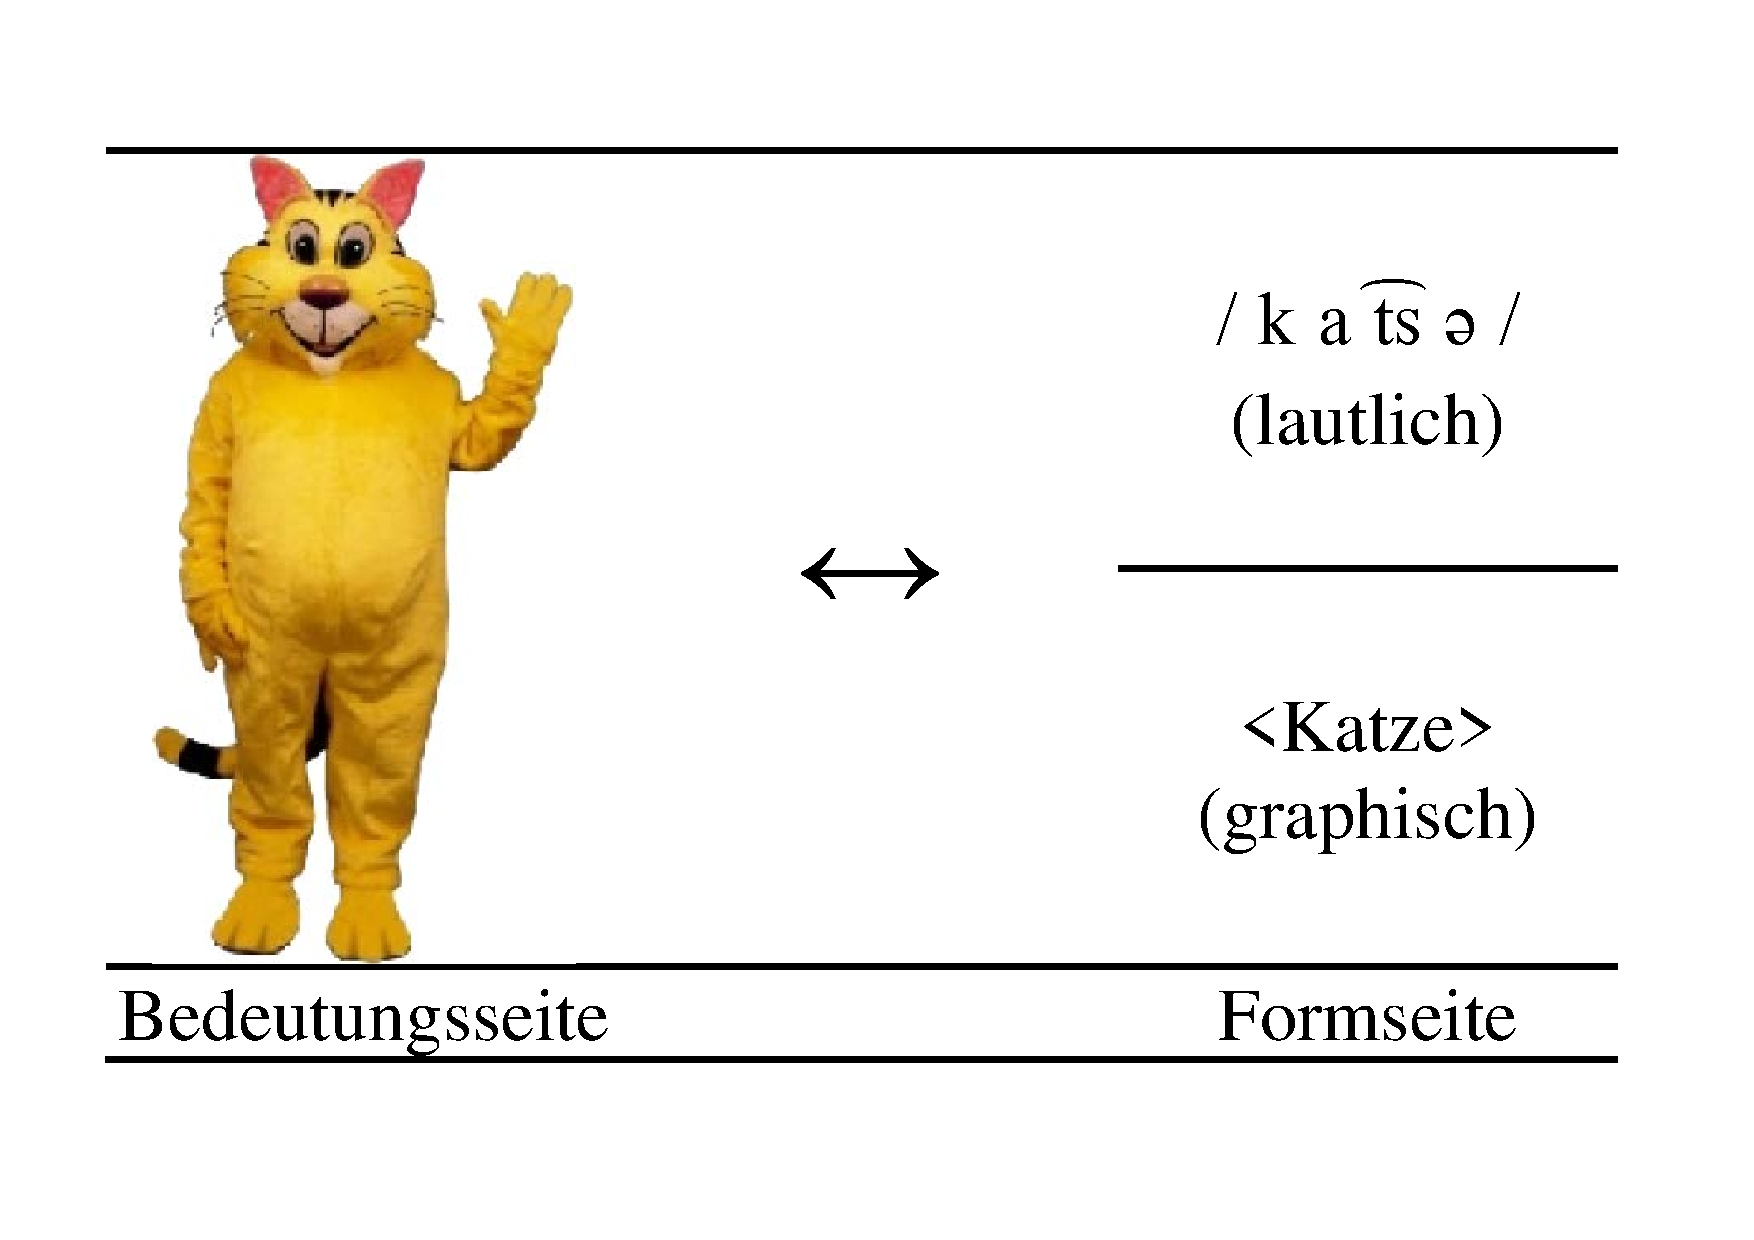
\includegraphics[scale=0.15]{material/01SSZeichenKatze}
%\caption{Beziehung zwischen Funktions-/Bedeutungs- und Formseite}
%\label{Zeichen1}
%\end{figure}

\end{frame}			


%%%%%%%%%%%%%%%%%%%%%%%%%%%%%%%%%%%
%Alternative zur Gelben Katze:

\begin{frame}
\frametitle{Sprachliche Zeichen: Form-Bedeutung-Paare}
\begin{table}
\huge
\centering
%\caption[Hauskatze]{https://commons.wikimedia.org/wiki/File:Hauskatze_an_einem_Scheunenfenster_in_Grossarl.JPG; Autor: Usien; GNU Free Documentation Licence}
\begin{tabular}{lp{1em}l}
\hline
\multirow{4}*{
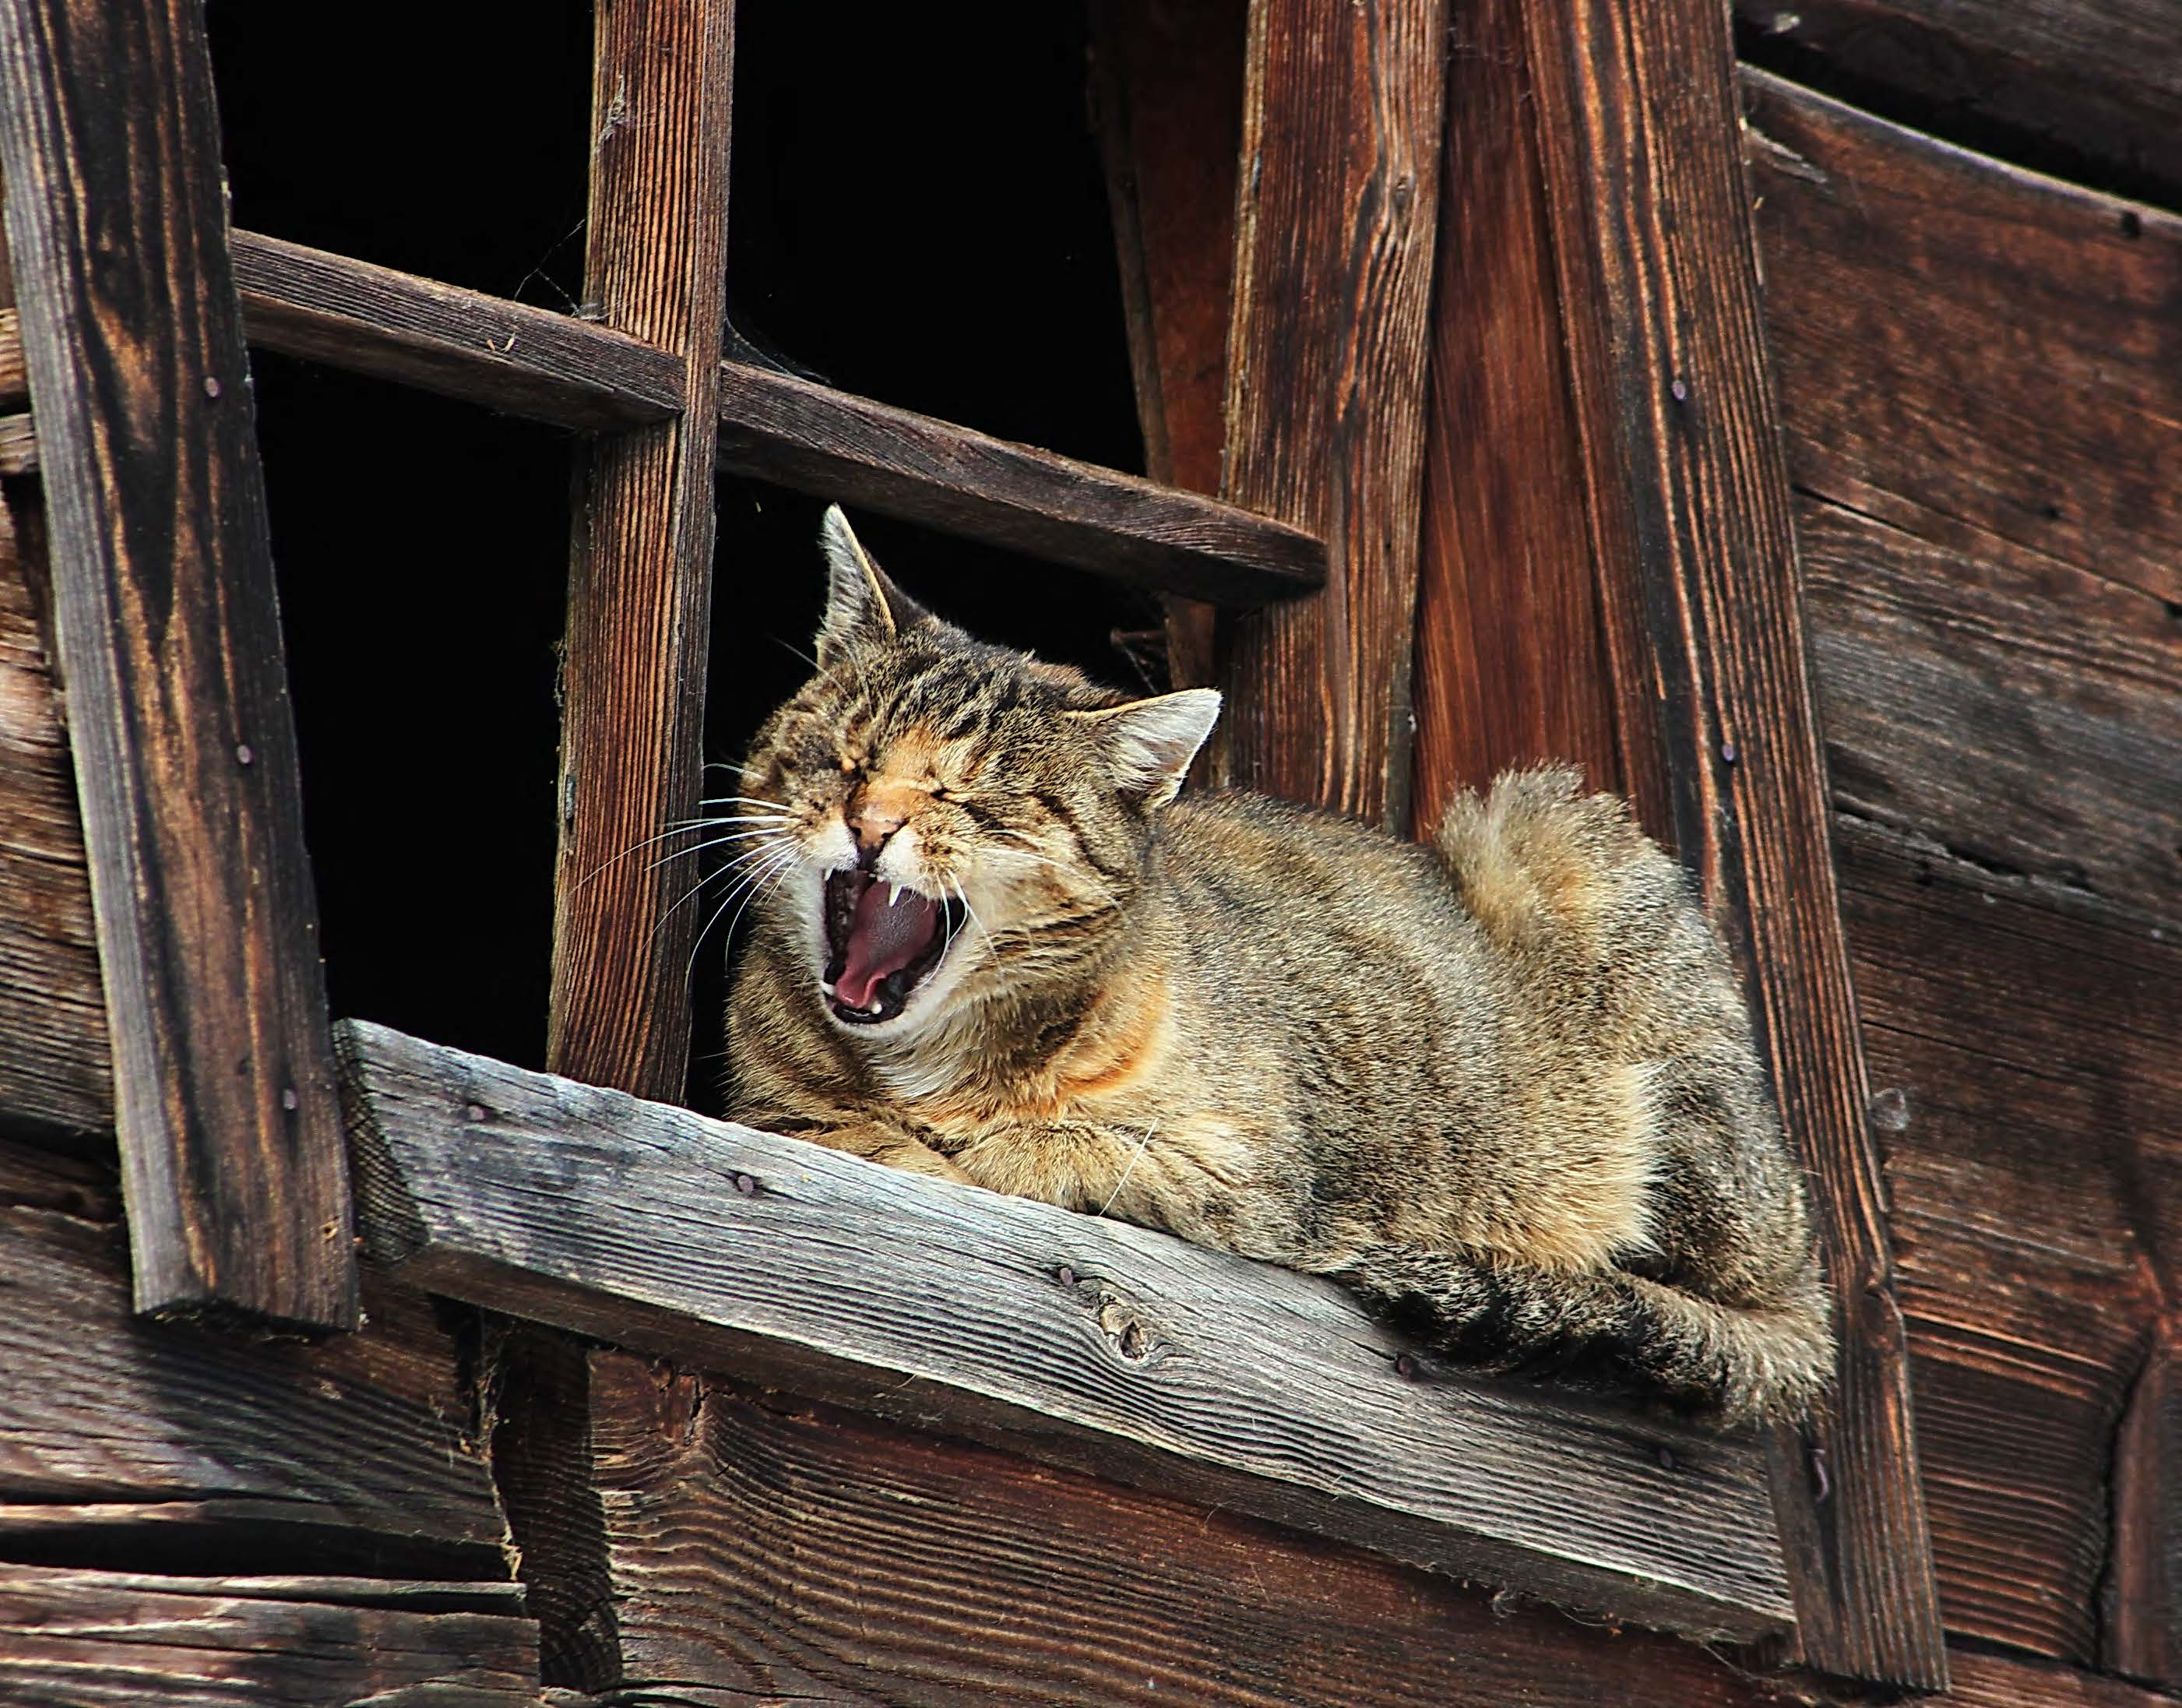
\includegraphics[scale=0.04]{material/Hauskatze-an-einem-Scheunenfenster-in-Grossarl}
}&  
%fehlt noch im Material-Ordner
\multirow{4}{6em}{{\Large $ \leftrightarrow $}} & / \textipa{k a \t{ts} \textschwa} / \\
                                              & &{\normalsize (lautlich)}\\
\cline{3-3}
& & $\langle$ Katze $\rangle$ \\
& & {\normalsize (graphisch)} \\
\hline
{\Large Bedeutungsseite} & & {\Large Formseite}\\
\hline \\
\end{tabular}
\end{table}

\hfill \dots vgl. \citet{Saussure16x}

\end{frame}


%%%%%%%%%%%%%%%%%%%%%%%%%%%%%%%%%%%
\begin{frame}
\frametitle{Zeichensysteme in der Tierkommunikation}

\begin{itemize}
	\item<1-> Tiere verwenden auch Zeichensysteme zur Kommunikation.
\end{itemize}			
			
%\begin{figure}[H]
%\centering

%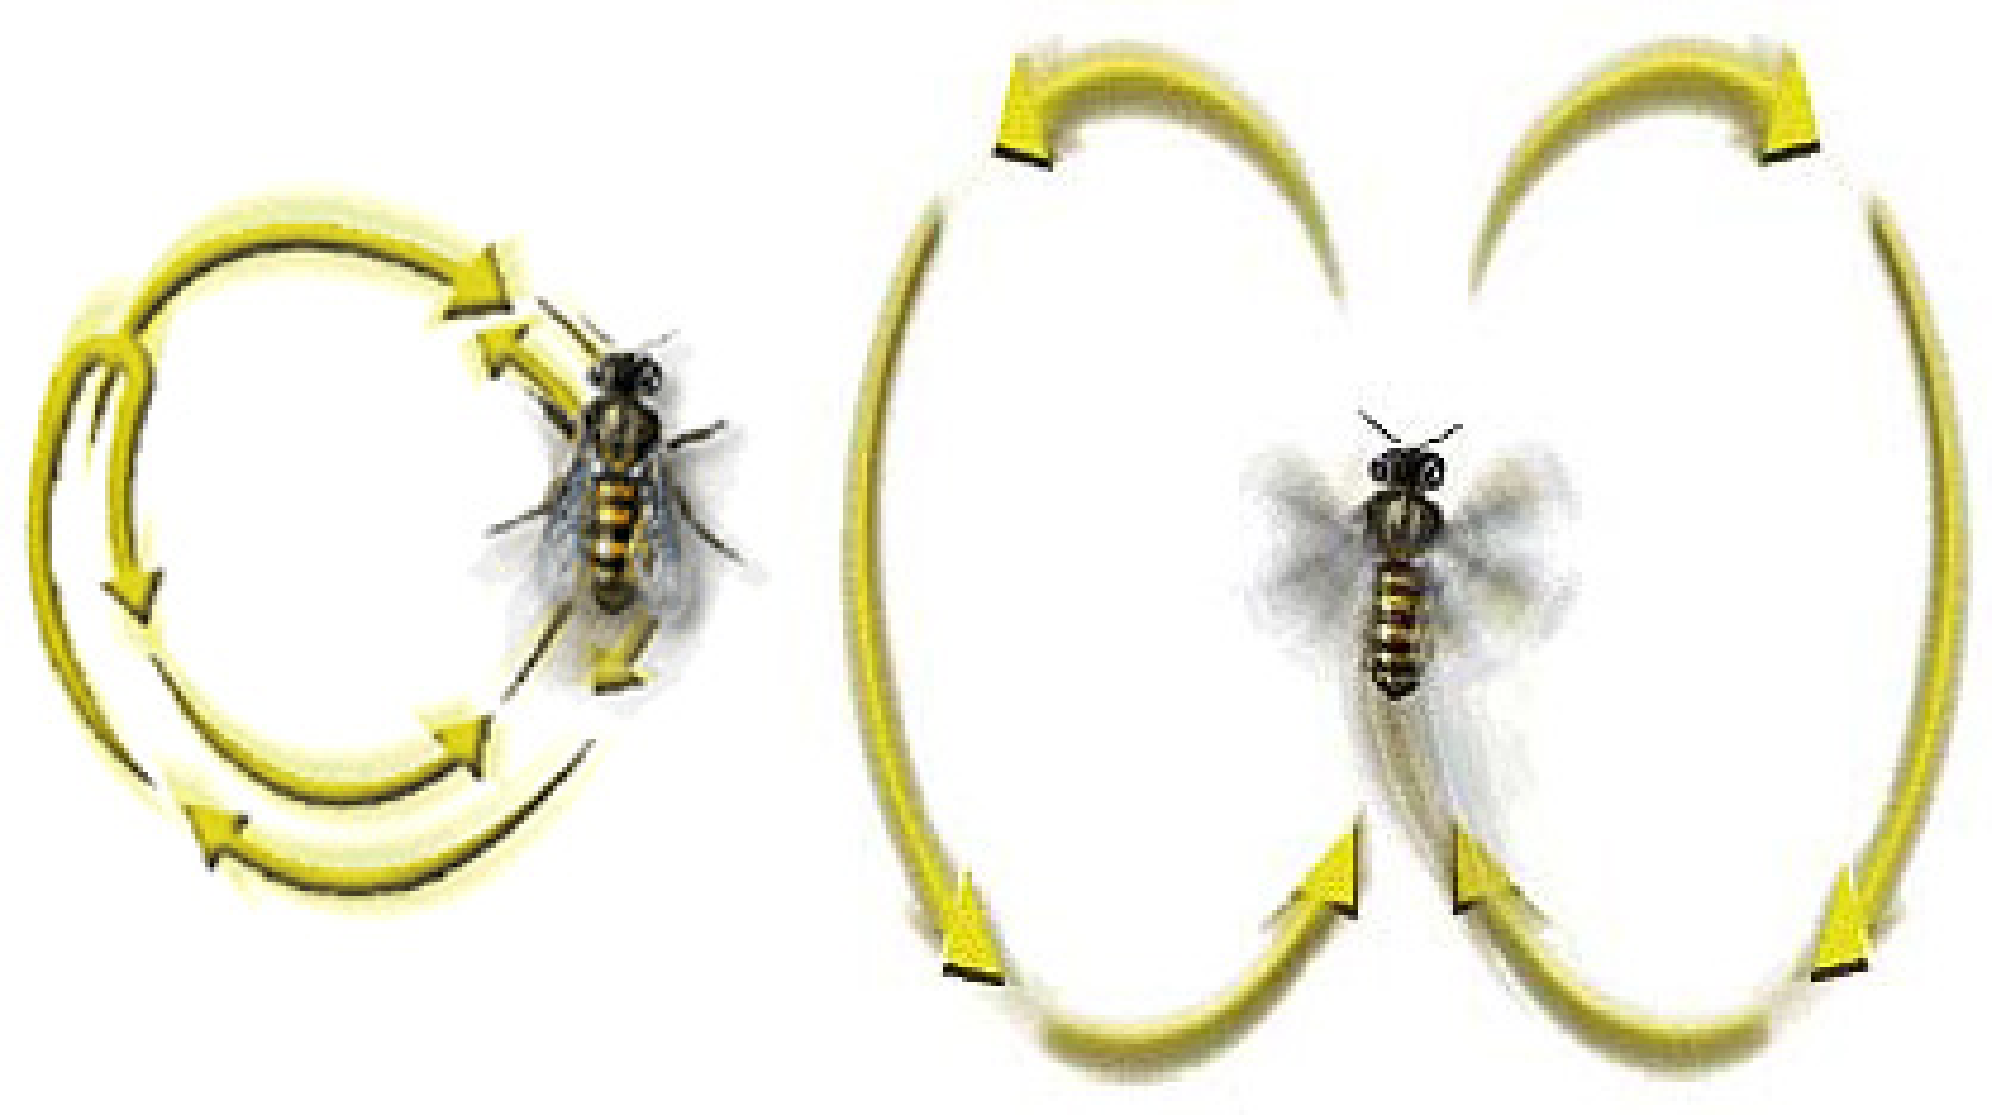
\includegraphics[scale=0.15]{material/01SSBienentanz}
%\caption{\gqq{Rundtanz} und \gqq{Schwänzeltanz} der Bienen}
%\label{Zeichen2}
%\end{figure}



\begin{itemize}
	\item<2-> Mit diesem Zeichensystem teilen Bienen die \textbf{Richtung} und \textbf{Entfernung} der nächsten Nahrungsquelle mit. 
	\item<2-> \textbf{Rundtanz:} Trachtgebiet in der Nähe (weniger als 25\,m)
	\item<2-> \textbf{Schwänzeltanz:} Trachtgebiet bis zu 10\,km weit entfernt, weitere Bewegungen zeigen die Richtung an.

\begin{figure}[H]
\centering
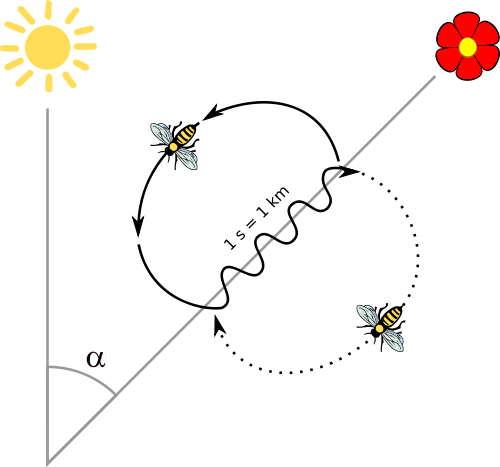
\includegraphics[scale=0.14]{material/Bee-dance}
%\caption{https://commons.wikimedia.org/wiki/File:Bee\_dance.png?uselang=de; GNU-Lizenz; Autor:Audriusa; Bee\_dance/Schwänzeltanz}
\label{Zeichen2}
\end{figure}

\end{itemize}		
		
\end{frame}			


%%%%%%%%%%%%%%%%%%%%%%%%%%%%%%%%%%%
\begin{frame}
\frametitle{Schwänzeltanz}

More than Honey. (R: Markus Imhoof, 2012), 13min 50sec.
%Quelle?

\end{frame}


%%%%%%%%%%%%%%%%%%%%%%%%%%%%%%%%%%%
%%%%%%%%%%%%%%%%%%%%%%%%%%%%%%%%%%%
\subsection{Merkmale natürlicher Sprachen}

%% MyP: Contents
\iftoggle{sectoc}{
	\frame{
		%\begin{multicols}{2}
		\frametitle{~}
		\tableofcontents[currentsubsection, subsubsectionstyle=hide]
		%\end{multicols}
	}
}

%% StM: Contents
\iftoggle{gliederung}{
	
	\outline{
		\begin{itemize}
			
			\item Ziel des Kurses
			\item Sprache und natürliche Sprache
			\item Zeichensysteme
			\item \blaubf{Merkmale natürlicher Sprachen}
			%% Bidirektionalität
			%% Situationelle Ungebundenheit
			%% Rückkopplung
			%% Diskretheit
			%% Produktivität
			%% Arbitrarität
			%% Fazit
			
		\end{itemize}
	}
}
%%%%%%%%%%%%%%%%%%%%%%%%%%%%%%%%%%%
	
\begin{frame}{Merkmale natürlicher Sprachen}

\begin{itemize}
	\item Die menschliche (natürliche) Sprache unterscheidet sich jedoch von anderen Zeichensystemen, wie der \gqq{Bienensprache} oder den Verkehrszeichen, \textbf{nicht in einem einzelnen Merkmal}, sondern \textbf{in einem Bündel von Merkmalen}, welche alle zusammen vorhanden sein müssen (vgl. \citealp{Hockett60a}).
\end{itemize}

\end{frame}


%%%%%%%%%%%%%%%%%%%%%%%%%%%%%%%%%%%
%%%%%%%%%%%%%%%%%%%%%%%%%%%%%%%%%%%
\subsubsection{Bidirektionalität}
%%% MyP: Contents
%\iftoggle{sectoc}{
%	\frame{
%		%\begin{multicols}{2}
%		\frametitle{~}
%		\tableofcontents[currentsubsubsection]
%		%\end{multicols}
%	}
%}
%%%%%%%%%%%%%%%%%%%%%%%%%%%%%%%%%%%

\begin{frame}{Bidirektionalität:}

	\begin{itemize}
		\item[]
		\item<1-> Mensch ist \textbf{sowohl Sender als auch Empfänger} eines Sprachsignals.
		\item[]
		\item<2-> Bei einigen Singvögeln ist das anders:
		
		\begin{itemize}
			\item[]
			\item[$\rightarrow$]<2-> Männchen singen zur Reviermarkierung oder um
                          Weibchen anzulocken.\\
                         Weibchen können oft nicht oder nur wenig singen.\\
                         Sie verstehen den Gesang der Männchen, können ihn aber selbst nicht produzieren.
		\end{itemize}
			
	\end{itemize}

\end{frame}


%%%%%%%%%%%%%%%%%%%%%%%%%%%%%%%%%%%
%%%%%%%%%%%%%%%%%%%%%%%%%%%%%%%%%%%
\subsubsection{Situationelle Ungebundenheit}
%%% MyP: Contents
%\iftoggle{sectoc}{
%	\frame{
%		%\begin{multicols}{2}
%		\frametitle{~}
%		\tableofcontents[currentsubsubsection]
%		%\end{multicols}
%	}
%}
%%%%%%%%%%%%%%%%%%%%%%%%%%%%%%%%%%%

\begin{frame}{Situationelle Ungebundenheit:}
	
	\begin{itemize}
		\item[]
		\item<1-> Menschen sind in der Lage auch über Dinge zu kommunizieren,\\
                          die \textbf{nicht hier und jetzt} stattfinden.
		
		\begin{itemize}
			\item[$\rightarrow$]<2-> Wir können über das leckere gestrige Essen in der Mensa und über unsere Freude auf das morgige Mensafestmahl reden.
		\end{itemize}
		\item<3-> Der Tanz der Bienen ist in diesem Fall der menschlichen Kommunikation ähnlich.
		\item<3-> Einige Primaten sind jedoch nur in der Lage über das Hier und Jetzt zu kommunizieren.
	\end{itemize}
		
\end{frame}


%%%%%%%%%%%%%%%%%%%%%%%%%%%%%%%%%%%
%%%%%%%%%%%%%%%%%%%%%%%%%%%%%%%%%%%
\subsubsection{Rückkopplung}
%%% MyP: Contents
%\iftoggle{sectoc}{
%	\frame{
%		%\begin{multicols}{2}
%		\frametitle{~}
%		\tableofcontents[currentsubsubsection]
%		%\end{multicols}
%	}
%}
%%%%%%%%%%%%%%%%%%%%%%%%%%%%%%%%%%%

\begin{frame}{Rückkopplung}
	
	\begin{itemize}
		\item<1-> Menschen können ihre \textbf{eigenen Sprachsignale} wahrnehmen und darauf reagieren.
		
\ea Ich habe heute \ldots ääähhhh GESTERN die Hausaufgaben abgegeben.
\z

\begin{itemize}
	\item<2->[$\rightarrow$] Der dreistachlige Stichling kann z.\,B. nicht die Färbung seiner Augen und seines Bauches wahrnehmen, die im Balzverhalten eine große Rolle spielt.
\end{itemize}
			\item[]
		\end{itemize}

\end{frame}


%%%%%%%%%%%%%%%%%%%%%%%%%%%%%%%%%%
%%%%%%%%%%%%%%%%%%%%%%%%%%%%%%%%%%
\subsubsection{Diskretheit}
%%% MyP: Contents
%\iftoggle{sectoc}{
%	\frame{
%		%\begin{multicols}{2}
%		\frametitle{~}
%		\tableofcontents[currentsubsubsection]
%		%\end{multicols}
%	}
%}
%%%%%%%%%%%%%%%%%%%%%%%%%%%%%%%%%%%

\begin{frame}{Diskretheit}
			
	\begin{itemize}
		\item Zeichen in natürlichen Sprachen können in kleine, diskrete (\textbf{voneinander unterscheidbare}) \textbf{Einheiten} zerlegt werden.

\pause
				
		\begin{itemize}
			\item[]
			\item[$\rightarrow$] \ab{Alben} und \ab{Alpen} unterscheiden sich nur in der Aussprache eines einzelnen Lautes.
			
			\ea \textipa{[\textglotstop{}al}{\red b}\textipa{@n]} vs. \textipa{[\textglotstop{}al}{\red p}\textipa{@n]}
			\z 
			
			\item[$\rightarrow$] Der Bienentanz ist eher kontinuierlich als diskret.						
		\end{itemize}
	
	\end{itemize}

\end{frame}


%%%%%%%%%%%%%%%%%%%%%%%%%%%%%%%%%%%
%%%%%%%%%%%%%%%%%%%%%%%%%%%%%%%%%%%
\subsubsection{Produktivität}
%%% MyP: Contents
%\iftoggle{sectoc}{
%	\frame{
%		%\begin{multicols}{2}
%		\frametitle{~}
%		\tableofcontents[currentsubsubsection]
%		%\end{multicols}
%	}
%}
%%%%%%%%%%%%%%%%%%%%%%%%%%%%%%%%%%%

\begin{frame}{Produktivität}
	
	\begin{itemize}
		\item<1-> Eins der wichtigsten Merkmale natürlicher Sprachen!
%		\item[]
		\item<2-> Aus einer \textbf{begrenzten Menge} von \textbf{Lauten} wird eine von
                  Menschen nicht überschaubare Menge von \textbf{Wörtern} und daraus eine unüberschaubare Menge von \textbf{Sätzen} produziert ($\rightarrow$ offenes oder produktives System).
%		\item[]
		\item<2-> Menschen können noch nie gehörte Sätze verstehen und noch nie gesagte Sätze produzieren.

\pause

\ea Meine Freundin hat gestern einen Wasserkocher mit Treueherzen von Kaiser's gekauft.
\ex Meine Freundin von Kaiser's hat gestern Treueherzen mit einem Wasserkocher gekauft.
\z
				
	\item<3-> Der Gibbon (kleiner Menschenaffe) hat ein geschlossenes Rufsystem mit einem kleinen \textbf{endlichen Inventar} an bekannten Lauten. 
	
	\end{itemize}
\end{frame}


%%%%%%%%%%%%%%%%%%%%%%%%%%%%%%%%%%%
%%%%%%%%%%%%%%%%%%%%%%%%%%%%%%%%%%%
\subsubsection{Arbitrarität}
%%% MyP: Contents
%\iftoggle{sectoc}{
%	\frame{
%		%\begin{multicols}{2}
%		\frametitle{~}
%		\tableofcontents[currentsubsubsection]
%		%\end{multicols}
%	}
%}
%%%%%%%%%%%%%%%%%%%%%%%%%%%%%%%%%%%

\begin{frame}{Arbitrarität}

\begin{itemize}
	\item<1-> \textbf{Bezeichnendes} (Signifikant, frz.\ signifiant) ist nicht durch \textbf{Bezeichnetes} (Signifikat, frz. signifié) bestimmt.
	\item[]
	\item<2-> Verschiedene Sprachen haben unterschiedliche Namen (Bezeichnendes) für das gleiche Objekt (Bezeichnetes):

\pause

\ea dt. \ab{Stift}, engl. \ab{pen}, sp. \ab{bolígrafo}, frz. \ab{crayon}, \ldots
\z

\pause 

	\item Benennung ist \textbf{konventionell}, \dash in der Sprachgemeinschaft festgelegt.

	\begin{itemize}
		\item[$\rightarrow$] Der Tanz der Bienen ist nicht arbiträr, sondern motiviert.
	\end{itemize}

\pause
		
	\item Es gibt in natürlichen Sprachen \textbf{auch motivierte} Zeichen:

\ea Deutsch und Dänisch \textipa{[va\textupsilon{} va\textupsilon{}]}, Griechisch \textipa{[gav gav]}, Russisch \textipa{[gaf gaf]}, Spanisch \textipa{[g\textupsilon{}au g\textupsilon{}au]}, Französisch \textipa{[g\textupsilon{}af g\textupsilon{}af]}, Englisch \textipa{[w\textopeno{}f w\textopeno{}f]}, Litauisch \textipa{[a\textupsilon{} a\textupsilon{}]}, Koreanisch \textipa{[m\textopeno{}N m\textopeno{}N]}
\z

\end{itemize}

\end{frame}


%%%%%%%%%%%%%%%%%%%%%%%%%%%%%%%%%%%
%%%%%%%%%%%%%%%%%%%%%%%%%%%%%%%%%%%
\subsubsection{Fazit}
%%% MyP: Contents
%\iftoggle{sectoc}{
%	\frame{
%		%\begin{multicols}{2}
%		\frametitle{~}
%		\tableofcontents[currentsubsubsection]
%		%\end{multicols}
%	}
%}
%%%%%%%%%%%%%%%%%%%%%%%%%%%%%%%%%%%
\begin{frame}{Fazit}
		
	\begin{block}{Natürliche Sprache}
			Insgesamt bildet die natürliche Sprache also ein \textbf{produktives}, \textbf{bidirektionales}, \textbf{arbiträres} und \textbf{diskretes} Symbolsystem (vgl. \citealp{Luedeling2009a}).
	\end{block}

\end{frame}	

%%%%%%%%%%%%%%%%%%%%%%%%%%%%%%%%%%%
%\begin{frame}{Übung}
%	Wie unterscheiden sich Computersprachen von natürlichen Sprachen? Diskutieren Sie dies anhand der eingeführten Kriterien.
%\end{frame}
%
%%%%%%%%%%%%%%%%%%%%%%%%%%%%%%%%%%%
%\iftoggle{ue-loesung}{
%	
%\begin{frame}{Übung -- Lösung}
%Wie unterscheiden sich Computersprachen von natürlichen Sprachen? Diskutieren Sie dies anhand der eingeführten Kriterien.
%
%{\red
%	
%\begin{itemize}
%\item Produktivität: ja, 
%\item Bidirektionalität:
%\item Arbitrarität: 
%\item Diskretheit: 
%\end{itemize}
%
%}
%
%\end{frame}
%
%}

%%%%%%%%%%%%%%%%%%%%%%%%%%%%%%%%%%%
%%%%%%%%%%%%%%%%%%%%%%%%%%%%%%%%%%%
\subsection*{Quellen}
%%%%%%%%%%%%%%%%%%%%%%%%%%%%%%%%%%%

\begin{frame}{Quellen}
	
	
	\begin{itemize}
		\item ABBILDUNG -- \gqq{Hauskatze} (Zugriff: 02.08.2019): \url{https://commons.wikimedia.org/wiki/File:Hauskatze\_an\_einem\_Scheunenfenster\_in\_Grossarl.JPG}
		%\medskip
		\item ABBILDUNG -- \gqq{Bienentanz} (Zugriff: 02.08.2019):
		\url{https://commons.wikimedia.org/wiki/File:Bee\_dance.png?uselang=de}
                \item VIDEO -- 	\textit{More than Honey}. Regie: Markus Imhoof. Drehbuch: Markus Imhoof, Kerstin Hoppenhaus. Schweiz/Deutschland/Österreich 2012. Fassung: DVD, 95 Min.
	\end{itemize}	
	
\end{frame}


%% %%%%%%%%%%%%%%%%%%%%%%%%%%%%%%%%%%%
%% %%%%%%%%%%%%%%%%%%%%%%%%%%%%%%%%%%%
%% \subsection*{Elektronische Quellen}
%% %%%%%%%%%%%%%%%%%%%%%%%%%%%%%%%%%%%

%% \begin{frame}{Elektronische Quellen}
	
	
	
%% 	\begin{itemize}
%% 		\item VIDEO -- 	\textit{More than Honey}. Regie: Markus Imhoof. Drehbuch: Markus Imhoof, Kerstin Hoppenhaus. Schweiz/Deutschland/Österreich 2012. Fassung: DVD, 95 Min.
%% 	\end{itemize}
	
%% \end{frame}


%%%%%%%%%%%%%%%%%%%%%%%%%%%%%%%%%%%%%%%%%%%%%%%%
%% Compile the master file!
%% 		Slides: Antonio Machicao y Priemer
%% 		Course: GK Linguistik
%%%%%%%%%%%%%%%%%%%%%%%%%%%%%%%%%%%%%%%%%%%%%%%%


%%%%%%%%%%%%%%%%%%%%%%%%%%%%%%%%%%%%%%%%%%%%%%%%%%%%
%%%             Metadata                         
%%%%%%%%%%%%%%%%%%%%%%%%%%%%%%%%%%%%%%%%%%%%%%%%%%%%      

\title{Grundkurs Linguistik}

\subtitle{Sprache \& Sprachwissenschaft II}

\author[aMyP]{
	{\small Antonio Machicao y Priemer}
	\\
	{\footnotesize \url{http://www.linguistik.hu-berlin.de/staff/amyp}}
	%	\\
	%	\href{mailto:mapriema@hu-berlin.de}{mapriema@hu-berlin.de}}
}

\institute{Institut für deutsche Sprache und Linguistik}

\date{ }

%\publishers{\textbf{6. linguistischer Methodenworkshop \\ Humboldt-Universität zu Berlin}}

%\hyphenation{nobreak}


%%%%%%%%%%%%%%%%%%%%%%%%%%%%%%%%%%%%%%%%%%%%%%%%%%%%
%%%             Preamble's End                   
%%%%%%%%%%%%%%%%%%%%%%%%%%%%%%%%%%%%%%%%%%%%%%%%%%%%       


%%%%%%%%%%%%%%%%%%%%%%%%%      
\huberlintitlepage

\iftoggle{toc}{
\frame{
\begin{multicols}{2}
	\frametitle{Inhaltsverzeichnis}
	\tableofcontents
	%[pausesections]
\end{multicols}
	}
	}

%%%%%%%%%%%%%%%%%%%%%%%%%%%%%%%%%%
%%%%%%%%%%%%%%%%%%%%%%%%%%%%%%%%%%
%%%%%LITERATURE:

%% Allgemein
\nocite{Glueck&Roedel16a}
\nocite{Schierholz&Co18}
\nocite{Luedeling2009a}
\nocite{Meibauer&Co07a} 
\nocite{Repp&Co15a} 

%% Sprache & Sprachwissenschaft
\nocite{Fries16c} %Adäquatheit
\nocite{Fries16a} %Grammatikalität
\nocite{Fries&MyP16c} %GG
\nocite{Fries&MyP16b} %Akzeptabilität
\nocite{Fries&MyP16d} %Kompetenz vs. Performanz


%%%%%%%%%%%%%%%%%%%%%%%%%%%%%%%%%%%
%%%%%%%%%%%%%%%%%%%%%%%%%%%%%%%%%%%
\section{Sprache \& Sprachwissenschaft II}

%%%%%%%%%%%%%%%%%%%%%%%%%%%%%%%%%%%
	
	
%%%%%%%%%%%%%%%%%%%%%%%%%%%%%%%%%%%
%%%%%%%%%%%%%%%%%%%%%%%%%%%%%%%%%%%
\subsection{Grammatik}
%% MyP: Contents
\iftoggle{sectoc}{
\frame{
%\begin{multicols}{2}
\frametitle{~}
	\tableofcontents[currentsubsection, subsubsectionstyle=hide]
%\end{multicols}
}
}

%% StM: Contents
\iftoggle{gliederung}{
	
	\outline{
		\begin{itemize}
			
			\item \blaubf{Grammatik}
			\item Grammatikbegriff
			\item Modularität der Grammatik
			%% Lexikon
			%% Phonologische Komponente
			%% Morphologische Komponente
			%% Syntaktische Komponente
			%% Semantische Komponente
			%% Architektur des Sprachsystems
			\item Linguistische Teildisziplinen
			\item Linguistik als Geistes- und/oder Naturwissenschaft
			\item Sprachwissenschaft \vs Linguistik
			
		\end{itemize}
	}
}
%%%%%%%%%%%%%%%%%%%%%%%%%%%%%%%%%%%
	
\begin{frame}{Grammatik}
	\begin{itemize}
		\item Komplexität des Sprachsystems (Einheiten + Regeln) ist den Sprechern meist \textbf{nicht bewusst}.
		\item[]
		\item Die Linguistik interessiert sich für das unbewusste, internalisierte System $\rightarrow$ sprachliche \textbf{Kompetenz} der Sprecher
		\item[]
		\item Diese Kompetenz bildet die Grammatik einer Sprache.
	\end{itemize}
	
	\begin{block}<2->{Grammatik}
		System, das Laute und Bedeutungen \textbf{regelhaft einander zuordnet} und das gesamte Regelsystem einer Sprache umfasst.
	\end{block}	
\end{frame}


%%%%%%%%%%%%%%%%%%%%%%%%%%%%%%%%%%%
%%%%%%%%%%%%%%%%%%%%%%%%%%%%%%%%%%%
\subsection{Grammatikbegriff}

%% MyP: Contents
\iftoggle{sectoc}{
\frame{
%\begin{multicols}{2}
\frametitle{~}
	\tableofcontents[currentsubsection, subsubsectionstyle=hide]
%\end{multicols}
}
}

%% StM: Contents
\iftoggle{gliederung}{
	
	\outline{
		\begin{itemize}
			
			\item Grammatik
			\item \blaubf{Grammatikbegriff}
			\item Modularität der Grammatik
			%% Lexikon
			%% Phonologische Komponente
			%% Morphologische Komponente
			%% Syntaktische Komponente
			%% Semantische Komponente
			%% Architektur des Sprachsystems
			\item Linguistische Teildisziplinen
			\item Linguistik als Geistes- und/oder Naturwissenschaft
			\item Sprachwissenschaft \vs Linguistik
			
		\end{itemize}
	}
}
%%%%%%%%%%%%%%%%%%%%%%%%%%%%%%%%%%%

\begin{frame}{Grammatikbegriff}

\begin{itemize}
	\item<1-> Grammatik im engeren Sinne als \textbf{Lehre} von morphologischen und syntaktischen Regularitäten einer Sprache. Unter dieser Auffassung bleiben die Phonologie und die Semantik als Teilbereiche der Sprachwissenschaft ausgeklammert (traditionelle Definition).
	\item[]
	\item<2-> Grammatik als \textbf{präskriptive/normative} Grammatik, die Vorgaben für die \gqq{korrekte} Sprachverwendung einer einzelnen Sprache (\gqq{gutes Deutsch}) macht (\zB \citealp{DudenGramm09d}).
	\item[]
	\item<3-> Grammatik als \textbf{deskriptive} Grammatik, die eine wertungsfreie Beschreibung einer einzelnen Sprache gibt (\zB \citealp{Eisenberg00a}, auch \gqq{Problemgrammatik} genannt).
\end{itemize}

\end{frame}


%%%%%%%%%%%%%%%%%%%%%%%%%%%%%%%%%%%
\begin{frame}

\begin{itemize}
	\item<1-> Grammatik als \textbf{Lehrbuch} oder \textbf{Nachschlagewerk}
	\item[]
	\item<2-> Grammatik für den Fremdsprachenunterricht (\zB \citealp{Helbig&Buscha05a})
	\item[]
	\item<3-> Grammatik als \textbf{Sprachtheorie}, \zB Generative Grammatik (GG) (vgl. \citealp{Philippi&Tewes10a}) oder Dependenzgrammatik (vgl. \citealp{Agel00a})
	\item[]
	\item<4-> In diesem Seminar verstehen wir Grammatik als:

	\begin{itemize}
		\item<4-> \textbf{System}, das Laute und Bedeutungen regelhaft einander zuordnet und das gesamte Regelsystem einer Sprache umfasst.
		\item<4-> Wir befassen uns mit Grammatik mit einer \textbf{deskriptiven} Methodik
                  (d.\,h. nicht präskriptiv!) und verwenden dafür (bzw. bilden dadurch)
                  \textbf{Grammatiktheorien} (z.\,B. GG).
	\end{itemize}

\end{itemize}

\end{frame}


%%%%%%%%%%%%%%%%%%%%%%%%%%%%%%%%%%%
%%%%%%%%%%%%%%%%%%%%%%%%%%%%%%%%%%%
\subsection{Modularität der Grammatik}

%% MyP: Contents
\iftoggle{sectoc}{
\frame{
%\begin{multicols}{2}
\frametitle{~}
	\tableofcontents[currentsubsection, subsubsectionstyle=hide]
%\end{multicols}
}
}

%% StM: Contents
\iftoggle{gliederung}{
	
	\outline{
		\begin{itemize}
			
			\item Grammatik
			\item Grammatikbegriff
			\item \blaubf{Modularität der Grammatik}
			%% Lexikon
			%% Phonologische Komponente
			%% Morphologische Komponente
			%% Syntaktische Komponente
			%% Semantische Komponente
			%% Architektur des Sprachsystems
			\item Linguistische Teildisziplinen
			\item Linguistik als Geistes- und/oder Naturwissenschaft
			\item Sprachwissenschaft \vs Linguistik
			
		\end{itemize}
	}
}
%%%%%%%%%%%%%%%%%%%%%%%%%%%%%%%%%%%

\begin{frame}{Modularität der Grammatik}
	
\begin{itemize}
	\item hauptsächlich in der Generativen Grammatik angenommen\\
              (in anderen Grammatiktheorietraditionen umstritten)
	\item[]
	\item Sprachvermögen $\rightarrow$ modular organisiert
	\item<2-> Grammatik (oder Sprache) ist ein \textbf{Modul} im \textbf{menschlichen kognitiven System}.
	\item<2-> Dieses (Sprach)modul besteht zugleich aus \textbf{miteinander interagierenden Teilmodulen} (auch sprachlichen Teilmodulen, grammatischen Ebenen oder sprachlichen Komponenten)
	\item[]
	\item<3-> Wie \textbf{selbstständig} diese Module sind, ist umstritten.
	\item[]
	\item<3-> Die \textbf{Evidenz} für diese Modularisierung findet die GG in der Aphasie-, Versprecher- und Spracherwerbsforschung.  
\end{itemize}

\end{frame}


%%%%%%%%%%%%%%%%%%%%%%%%%%%%%%%%%%%
\begin{frame}
\frametitle{Module}
\begin{itemize}
	\item Folgende Module werden angenommen (vgl. \citealp{Abramowski2016}):
		
	\begin{itemize}
%		\item[]
		\item Lexikon
%		\item[]
		\item Phonologische Komponente
%		\item[]
		\item Morphologische Komponente
%		\item[]
		\item Syntaktische Komponente
%		\item[]
		\item Semantische Komponente
%		\item[]
	\end{itemize}
		
	\item<2-> Jedes sprachliche Modul besteht zugleich aus:
	
	\begin{enumerate}
		\item<2-> einem Inventar von komponentenspezifisch kategorisierten \textbf{Minimaleinheiten}\\
                         (\zB Morphem in der Morphologie) und
		\item<2-> einer Menge von komponentenspezifischen \textbf{Regeln zur Kombination} dieser Minimaleinheiten zu wohlgeformten komplexen Einheiten. 
	\end{enumerate}		  
		
\end{itemize}

\end{frame}


%%%%%%%%%%%%%%%%%%%%%%%%%%%%%%%%%%%
%%%%%%%%%%%%%%%%%%%%%%%%%%%%%%%%%%%
\subsubsection{Lexikon}
%%% MyP: Contents
%\iftoggle{sectoc}{
%	\frame{
%		%\begin{multicols}{2}
%		\frametitle{~}
%		\tableofcontents[currentsubsubsection]
%		%\end{multicols}
%	}
%}
%%%%%%%%%%%%%%%%%%%%%%%%%%%%%%%%%%%

\begin{frame}{Lexikon}
	
	\begin{itemize}
		\item \textbf{Repräsentation von Wörtern} und Wortteilen einer Sprache mit der \textbf{Information} über deren:

		\begin{enumerate}
			\item[]
			\item Aussprache (phonologische Information)
			\item[]
			\item interne Struktur (morphologische Information)
			\item[]
			\item syntaktische Kategorie und syntaktisches Kombinationspotential (syntaktische Information)
			\item[]
			\item Bedeutung (semantische Information) 
			\item[]
			\item idiosynkratische Information (nicht ableitbare Information)
		\end{enumerate}		  
			
	\end{itemize}
		
\end{frame}


%%%%%%%%%%%%%%%%%%%%%%%%%%%%%%%%%%%
\begin{frame}{Lexikon}
			
\begin{itemize}
	\item Eintrag für den Verbstamm \emph{geb-} (von \emph{geben}): \ab{\textsc{geb-}}

	\begin{enumerate}
		\item[]
		\item Phonologische Information: \textipa{/ge\textlengthmark{}b/}
		\item[]
		\item Morphologische Information: [\textsubscript{V-Stamm}\ab{geb-}] 
		\item[]
		\item Syntaktische Information (ditransitives Verb):\\
			NP\textsubscript{\alertred{1}\{\textsc{nom}\}}$+$
			NP\textsubscript{\alertred{2}\{\textsc{dat}\}}$+$
			NP\textsubscript{\alertred{3}\{\textsc{akk}\}}$+$
			V
					
		\item[]
		\item Semantische Information (Verb des Besitzwechsels):\\
			NP\textsubscript{\alertred{1}\{\textsc{agens}\}}$+$
			NP\textsubscript{\alertred{2}\{\textsc{goal}\}}$+$
			NP\textsubscript{\alertred{3}\{\textsc{thema}\}}$+$
			V \\
			$\approx$
			\gq{NP\textsubscript{\alertred{1}} macht, dass NP\textsubscript{\alertred{2}} NP\textsubscript{\alertred{3}} erhält.} 
	\end{enumerate}		  


\ea (\dots dass) Luise\MyPdown{\alertred{1}} Jacob\MyPdown{\alertred{2}} das Buch\MyPdown{\alertred{3}} gibt.
\z 
\end{itemize}

\end{frame}


%%%%%%%%%%%%%%%%%%%%%%%%%%%%%%%%%%%
%%%%%%%%%%%%%%%%%%%%%%%%%%%%%%%%%%%
\subsubsection{Phonologische Komponente}
%%% MyP: Contents
%\iftoggle{sectoc}{
%	\frame{
%		%\begin{multicols}{2}
%		\frametitle{~}
%		\tableofcontents[currentsubsubsection]
%		%\end{multicols}
%	}
%}
%%%%%%%%%%%%%%%%%%%%%%%%%%%%%%%%%%%

\begin{frame}{Phonologische Komponente}

	\begin{itemize}
		\item Sie beschränkt das \textbf{Lautinventar} einer Sprache.
		\item[]
		\item Sie regelt die \textbf{Lautkombinatorik} und \textbf{-veränderung}.
		\item[]
		\item Festlegung von \textbf{Wort-} und \textbf{Satzakzent}

		\begin{itemize}
			\item[]
			\item<2->[$\rightarrow$] Wieso spricht man \ab{Hund} mit \textipa{[t]} aber \ab{Hunde} mit \textipa{[d]} aus?
			\item[]
			\item<3->[$\rightarrow$] Kann ein Wort im Deutschen mit der Lautfolge \textipa{[Ng]} beginnen?
			\item[]
			\item<4->[$\rightarrow$] Was ist der Unterschied zwischen \abu{HAUStürgriff} und \abu{HausTÜRgriff}?
		\end{itemize}		  
	
	\end{itemize}
	
\end{frame}


%%%%%%%%%%%%%%%%%%%%%%%%%%%%%%%%%%%
%%%%%%%%%%%%%%%%%%%%%%%%%%%%%%%%%%%
\subsubsection{Morphologische Komponente}
%%% MyP: Contents
%\iftoggle{sectoc}{
%	\frame{
%		%\begin{multicols}{2}
%		\frametitle{~}
%		\tableofcontents[currentsubsubsection]
%		%\end{multicols}
%	}
%}
%%%%%%%%%%%%%%%%%%%%%%%%%%%%%%%%%%%

\begin{frame}{Morphologische Komponente}

\begin{itemize}
	\item Sie regelt die \textbf{interne Struktur von Wörtern}.
	\item[]
	\item Bildung von neuen Wörtern und Wortformen
				
	\begin{itemize}
		\item[]
		\item<2->[$\rightarrow$] Wie hängen \ab{kaufen} und \ab{kaufbar} zusammen?
		\item[]
		\item<3->[$\rightarrow$] Was zeigt \ab{-st} bei der Bildung neuer Verbformen an?
	\end{itemize}
			
\end{itemize}

\end{frame}


%%%%%%%%%%%%%%%%%%%%%%%%%%%%%%%%%%%
\begin{frame}{Morphologische Komponente}

	\begin{itemize}
		\item Warum ist die eine Struktur des Wortes \ab{Bedeutungsableitung} intuitiv nicht korrekt und die andere schon?
	\end{itemize}
			

\begin{columns}

\column[b]{.4\linewidth}		
\begin{figure}[b]
	
\scriptsize{
		\begin{forest}MyP edges
		[Bedeutungsableitung [Be][deutungsableitung [deut][ungsableitung [ungsableit [ung][sableit [sab [s][ab]][leit]]][ung]]]]
		\end{forest}
}
		
\caption{Ungrammatisch}

\end{figure}

\column[b]{.4\linewidth}
\begin{figure}[b]
	\scriptsize{
		\begin{forest}MyP edges
		[Bedeutungsableitung [Bedeutungs [Bedeutung [Bedeut [Be][deut]][ung]][s]][ableitung [ableit [ab][leit]][ung]]]
		\end{forest}}
			
	\caption{Grammatisch}

\end{figure}

\end{columns}
\end{frame}


%%%%%%%%%%%%%%%%%%%%%%%%%%%%%%%%%%%
%%%%%%%%%%%%%%%%%%%%%%%%%%%%%%%%%%%
\subsubsection{Syntaktische Komponente}
%%% MyP: Contents
%\iftoggle{sectoc}{
%	\frame{
%		%\begin{multicols}{2}
%		\frametitle{~}
%		\tableofcontents[currentsubsubsection]
%		%\end{multicols}
%	}
%}
%%%%%%%%%%%%%%%%%%%%%%%%%%%%%%%%%%%
	
\begin{frame}{Syntaktische Komponente}

\begin{itemize}
	\item Sie regelt die \textbf{Struktur} von \textbf{Phrasen und Sätzen}.

	\begin{enumerate}
		\item[]
		\item<2->[$\rightarrow$] Wieso ist die Phrase (\ref{ex1a}) grammatisch und die Phrase (\ref{ex1b}) nicht?
		
\eal
	\ex[ ]{die Königin von Schweden aus Deutschland}\label{ex1a}
	\ex[*]{die Königin aus Deutschland von Schweden}\label{ex1b}
	\zl
		\item<3->[$\rightarrow$] Warum ist ein Satz wie (\ref{ex2a}) ungrammatisch (trotz alphabetischer Anordnung der Wörter), während (\ref{ex2b}) grammatisch ist?

\eal
	\ex[*]{Buch Chomsky das ich kaufen morgen von werde.}\label{ex2a}
	\ex[]{Das Buch von Chomsky werde ich morgen kaufen.}\label{ex2b}
	\zl
	
		\item<4->[$\rightarrow$] Aus welchem Grund hat der Satz unter (\ref{ex3}) zwei Bedeutungen? 

\ea Maria hat Peter gesehen.\label{ex3}
\z

	\end{enumerate}
			
\end{itemize}

\end{frame}


%%%%%%%%%%%%%%%%%%%%%%%%%%%%%%%%%%%
%%%%%%%%%%%%%%%%%%%%%%%%%%%%%%%%%%%
\subsubsection{Semantische Komponente}
%%% MyP: Contents
%\iftoggle{sectoc}{
%	\frame{
%		%\begin{multicols}{2}
%		\frametitle{~}
%		\tableofcontents[currentsubsubsection]
%		%\end{multicols}
%	}
%}
%%%%%%%%%%%%%%%%%%%%%%%%%%%%%%%%%%%
		
\begin{frame}{Semantische Komponente}
	
	\begin{itemize}
		\item Semantische Komponente regelt die \textbf{Bedeutungsherleitung} komplexerer Einheiten (komplexer Wörter, Phrasen und Sätze).
%		\item[]
		\item<2-> Wichtig bei der Herleitung $\rightarrow$ \textbf{Bedeutung der Bestandteile + Bedeutung der Struktur} (Kompositionalitäts- oder \textbf{Fregeprinzip})
				
		\begin{enumerate}
			\item<3->[$\rightarrow$] Worin besteht der Bedeutungsunterschied zwischen den Verben \ab{arbeiten} und \ab{bearbeiten}?
			\item<4->[$\rightarrow$] Wieso haben die Sätze (\ref{ex4a}) und (\ref{ex4b})
                          nicht die gleiche Bedeutung,\\
wenn sie aus den gleichen Wörtern bestehen?

\eal	
	\ex Maria hat Peter gesehen. \label{ex4a}
	\ex Hat Maria Peter gesehen? \label{ex4b}
\zl

			\item<5->[$\rightarrow$] Warum bedeutet \ab{sich} in (\ref{ex5a}) und (\ref{ex5b}) nicht dasselbe?
	
\eal
	\ex Maria verspricht \textbf{sich}, Mario zu treffen. \label{ex5a}
	\ex Maria verspricht Mario, \textbf{sich} zu treffen. \label{ex5b}
\zl
		\end{enumerate}
	\end{itemize}
	
\end{frame}


%%%%%%%%%%%%%%%%%%%%%%%%%%%%%%%%%%%
%%%%%%%%%%%%%%%%%%%%%%%%%%%%%%%%%%%
\subsubsection{Architektur des Sprachsystems}
%%% MyP: Contents
%\iftoggle{sectoc}{
%	\frame{
%		%\begin{multicols}{2}
%		\frametitle{~}
%		\tableofcontents[currentsubsubsection]
%		%\end{multicols}
%	}
%}
%%%%%%%%%%%%%%%%%%%%%%%%%%%%%%%%%%%
		
\begin{frame}{Architektur des Sprachsystems}
	
	\begin{itemize}
		\item Sprachliche Strukturbildung wird durch bereits erwähnte Komponenten geregelt.
		\item[]
		\item<2-> Außerdem interagiert das grammatische System der Sprache mit den folgenden \textbf{außersprachlichen Ebenen}:
				
		\begin{itemize}
			\item[]
			\item<3-> dem \textbf{artikulatorisch-perzeptorischen Apparat}\par
				(den biologischen Gegebenheiten zur Produktion und Rezeption von Sprachlauten)
			\item[]
			\item<3->[] und
			\item[]
			\item<4-> dem \textbf{konzeptuell-intentionalen System}, d.\,h. dem Bereich der Kognition, der sich mit Bedeutung befasst.\par
				Das konzeptuell-intentionale System wird wiederum durch Weltwissen, Kontextwissen und analytisches Wissen gespeist.
		\end{itemize}
			
	\end{itemize}
		
\end{frame}


%%%%%%%%%%%%%%%%%%%%%%%%%%%%%%%%%%%
%\begin{frame}{Architektur des Sprachsystems}

%\begin{figure}[H]
%\centering
				
%	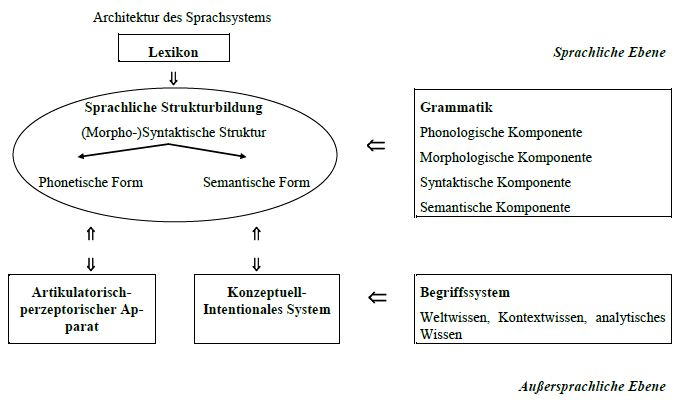
\includegraphics[width=\textwidth]{material/03ArchitekturSprachsystem.jpg}
%	\caption{Architektur des Sprachsystems \citep{Abramowski2016}}
%	\label{Zeichen3}

%\end{figure}

%\end{frame}			


%%%%%%%%%%%%%%%%%%%%%%%%%%%%%%%%%%%
\begin{frame}

\begin{figure}
\centering
\small
\begin{minipage}{0.55\textwidth}
\centering
\fbox{Lexikon}\\
\Large
$ \Downarrow $
\end{minipage}
%
\begin{minipage}{0.1\textwidth}
\centering
\hfill
\end{minipage}
%
\begin{minipage}[t]{0.3\textwidth}
\centering
\textit{Sprachliche Ebene}
\end{minipage}

\begin{minipage}[t]{0.55\textwidth}
\centering
\outputbox{\centering Sprachliche Strukturbildung\\
\begin{forest}sm edges,
[(morpho-)syntaktische Struktur
[Phonetische Form]
[Semantische Form]
]
\end{forest}}
\begin{tabular}{cp{3cm}c}
\Large
$ \Updownarrow $ && \Large $ \Updownarrow $\\
\end{tabular}
\end{minipage}
%
\begin{minipage}[c]{0.1\textwidth}
\centering
\Large
$ \Leftarrow $
\end{minipage}
%
\begin{minipage}[t]{0.3\textwidth}
\centering
\small
\outputbox{
Grammatik
\begin{itemize*}
\item Phonologische Komponente\\
\item Morphologische K.\\
\item Syntaktische K.\\
\item Semantische K.
\end{itemize*}}
\end{minipage}

\begin{minipage}{0.24\textwidth}
\centering
\outputbox{\centering Artikularisch-perzeptorischer Apparat}
\end{minipage}
%
\begin{minipage}[c]{0.05\textwidth}
\hfill
\end{minipage}
%
\begin{minipage}{0.24\textwidth}
\centering
\outputbox{\centering Konzeptuell-Intentionales System}
\end{minipage}
%
\begin{minipage}{0.1\textwidth}
\centering
\Large
$\Leftarrow$
\end{minipage}
%
\begin{minipage}{0.3\textwidth}
\outputbox{Begriffssystem
\newline
\small
\raggedright
Weltwissen, Kontextwissen, analytisches Wissen}
\end{minipage}

\begin{minipage}{0.65\textwidth}
\hfill
\end{minipage}
%
\begin{minipage}{0.3\textwidth}
\centering
\small
\textit{Außersprachliche Ebene}
\end{minipage}
\caption{Die Architektur des Sprachsystems \citep[vgl.][]{Abramowski2016}}
\end{figure}

\end{frame}


%%%%%%%%%%%%%%%%%%%%%%%%%%%%%%%%%%%
%%%%%%%%%%%%%%%%%%%%%%%%%%%%%%%%%%%
\subsection{Linguistische Teildisziplinen}		

%% MyP: Contents
\iftoggle{sectoc}{
\frame{
%\begin{multicols}{2}
	\tableofcontents[currentsubsection, subsubsectionstyle=hide]
%\end{multicols}
}
}

%% StM: Contents
\iftoggle{gliederung}{
	
	\outline{
		\begin{itemize}
			
			\item Grammatik
			\item Grammatikbegriff
			\item Modularität der Grammatik
			%% Lexikon
			%% Phonologische Komponente
			%% Morphologische Komponente
			%% Syntaktische Komponente
			%% Semantische Komponente
			%% Architektur des Sprachsystems
			\item \blaubf{Linguistische Teildisziplinen}
			\item Linguistik als Geistes- und/oder Naturwissenschaft
			\item Sprachwissenschaft \vs Linguistik
			
		\end{itemize}
	}
}
%%%%%%%%%%%%%%%%%%%%%%%%%%%%%%%%%%%

\begin{frame}{Linguistische Teildisziplinen}

	\begin{itemize}
		\item Phonologie
		\item Morphologie
		\item Syntax
		\item Semantik
		\item[]
		\item Phonetik
		\item Graphematik
		\item Pragmatik
		\item[]
		\item Psycholinguistik
		\item Soziolinguistik
		\item Historische Linguistik
		\item Korpuslinguistik
		\item \dots
	\end{itemize}
	
\end{frame}



%%%%%%%%%%%%%%%%%%%%%%%%%%%%%%%%%%%
%%%%%%%%%%%%%%%%%%%%%%%%%%%%%%%%%%%
\subsection{Linguistik als Geistes- und/oder Naturwissenschaft}		

%% MyP:Contents
\iftoggle{sectoc}{
\frame{
%\begin{multicols}{2}
	\tableofcontents[currentsubsection, subsubsectionstyle=hide]
%\end{multicols}
}
}

%% StM: Contents
\iftoggle{gliederung}{
	
	\outline{
		\begin{itemize}
			
			\item Grammatik
			\item Grammatikbegriff
			\item Modularität der Grammatik
			%% Lexikon
			%% Phonologische Komponente
			%% Morphologische Komponente
			%% Syntaktische Komponente
			%% Semantische Komponente
			%% Architektur des Sprachsystems
			\item Linguistische Teildisziplinen
			\item \blaubf{Linguistik als Geistes- und/oder Naturwissenschaft}
			\item Sprachwissenschaft \vs Linguistik
			
		\end{itemize}
	}
}
%%%%%%%%%%%%%%%%%%%%%%%%%%%%%%%%%%%

\begin{frame}{Linguistik als Geistes- und/oder Naturwissenschaft}

	\begin{itemize}
		\item \textbf{Geisteswissenschaft}
		
		\begin{itemize}
			\item Verstehen von individuellen Leistungen des Geistes\par
				(eines Menschen, einer Gemeinschaft, einer Epoche)
			\item Verstehen von kulturellen Beziehungen und Entwicklungen
			\item[$\rightarrow$] Methode: \textbf{Hermeneutik} (Annähern durch Verstehen)
		\end{itemize}
		
		\item[]
		\item \textbf{Naturwissenschaft}
		
		\begin{itemize}
			\item Erklärung von naturgesetzlichen Kausalitäten und Zusammenhängen
			\item[$\rightarrow$] Methode: \textbf{Experiment}
		\end{itemize}
		
	\end{itemize}
	
\end{frame}		


%%%%%%%%%%%%%%%%%%%%%%%%%%%%%%%%%%%
\begin{frame}
\frametitle{Linguistik als Naturwissenschaft}

	\begin{itemize}
		\item Linguistik \textit{eher} naturwissenschaftlich ausgerichtet\par
			(im Gegensatz zur Literaturwissenschaft)
		
		\begin{itemize}
			\item[]
			\item \textbf{Beobachtung} und \textbf{Analyse} von Gesetzen natürlicher Sprachen mit dem Ziel ihre \textbf{Systematik} aufzudecken (\zB Syntax)
			\item[]
			\item<2-> Arbeit mit \textbf{empirischen} Verfahren wie Experimenten (\zB Psycholinguistik) oder wie Ansammlungen von Daten (\zB Korpuslinguistik) als Evidenz $\rightarrow$ \textbf{Naturwissenschaft}
			\item[]
			\item<3-> Beschäftigung mit der \textbf{Geschichte} einer Sprache (\zB Historische Linguistik) und mit den \textbf{sozialen} und kulturellen Bedingungen vom Sprachwandel (\zB Soziolinguistik) $\rightarrow$ \textbf{Geisteswissenschaft}
			\item[]
			\item<4-> Untersuchung des vielleicht \textbf{zentralsten Outputs des Geistes}:\par
				der Sprache (vgl. \citealt{Meibauer&Co07a})
		\end{itemize}
		
	\end{itemize}
	
\end{frame}		


%%%%%%%%%%%%%%%%%%%%%%%%%%%%%%%%%%%
%%%%%%%%%%%%%%%%%%%%%%%%%%%%%%%%%%%
\subsection{Sprachwissenschaft \vs Linguistik}

%% MyP: Contents
\iftoggle{sectoc}{
\frame{
%\begin{multicols}{2}
	\tableofcontents[currentsubsection, subsubsectionstyle=hide]
%\end{multicols}
}
}

%% StM: Contents
\iftoggle{gliederung}{
	
	\outline{
		\begin{itemize}
			
			\item Grammatik
			\item Grammatikbegriff
			\item Modularität der Grammatik
			%% Lexikon
			%% Phonologische Komponente
			%% Morphologische Komponente
			%% Syntaktische Komponente
			%% Semantische Komponente
			%% Architektur des Sprachsystems
			\item Linguistische Teildisziplinen
			\item Linguistik als Geistes- und/oder Naturwissenschaft
			\item \blaubf{Sprachwissenschaft \vs Linguistik}
			
		\end{itemize}
	}
}
%%%%%%%%%%%%%%%%%%%%%%%%%%%%%%%%%%%

\begin{frame}{Sprachwissenschaft \vs Linguistik}

	\begin{itemize}
		\item<1-> Linguistik und Sprachwissenschaft \idR \textbf{synonymisch} gebraucht
%		\item[]
		\item<2-> Unterscheidung:
		
		\begin{itemize}
%			\item[]
			\item<2-> Linguistik als \textbf{Teildisziplin} der Sprachwissenschaft
			\item<3-> \gqq{\textbf{Innere Sprachwissenschaft}} $\approx$ Linguistik $\rightarrow$ Beschäftigung mit innersprachlichen Sachverhalten und Entwicklungen (Sprache als System)
			\item<4-> \gqq{\textbf{Äußere Sprachwissenschaft}} $\rightarrow$ Beschäftigung mit kulturellen, sozialen, ökonomischen, politischen, usw. Bedingungen der Existenz und der Geschichte von Sprache, d.\,h. den äußeren (auch \textit{außersprachlich} genannten) Faktoren (vgl. \citealp{Glueck05a})
		\end{itemize}
		
%		\item[]
		\item<5-> In diesem Kurs werden wir jedoch beide Begriffe gleichbedeutend verwenden.
	\end{itemize}
	
\end{frame}

%%%%%%%%%%%%%%%%%%%%%%%%%%%%%%%%%%%




%%%%%%%%%%%%%%%%%%%%%%%%%%%%%%%%%%%%%%%%%%%%%%%%%%%%
%%%             Metadata                         %%%
%%%%%%%%%%%%%%%%%%%%%%%%%%%%%%%%%%%%%%%%%%%%%%%%%%%%      

\title{Grundkurs Linguistik}

\subtitle{Phonetik\\
Sprechaktlautlehre}

\author[aMyP]{
	{\small Antonio Machicao y Priemer}
%	\\
%	{\footnotesize \url{http://www.linguistik.hu-berlin.de/staff/amyp}\\
%	\href{mailto:mapriema@hu-berlin.de}{mapriema@hu-berlin.de}}
}

\institute{Institut für deutsche Sprache und Linguistik}

%%%%%%%%%%%%%%%%%%%%%%%%%      
\date{ }
%\publishers{\textbf{6. linguistischer Methodenworkshop \\ Humboldt-Universität zu Berlin}}

%\hyphenation{nobreak}


%%%%%%%%%%%%%%%%%%%%%%%%%%%%%%%%%%%%%%%%%%%%%%%%%%%%
%%%             Preamble's End                   %%%
%%%%%%%%%%%%%%%%%%%%%%%%%%%%%%%%%%%%%%%%%%%%%%%%%%%%      


%%%%%%%%%%%%%%%%%%%%%%%%%      
\huberlintitlepage

\iftoggle{toc}{
\frame{
\begin{multicols}{2}
	\frametitle{Inhaltsverzeichnis}\tableofcontents
	%[pausesections]
\end{multicols}
}
}

%%%%%%%%%%%%%%%%%%%%%%%%%%%%%%%%%%%
%%%%%%%%%%%%%%%%%%%%%%%%%%%%%%%%%%

\nocite{Hall00a} 
\nocite{Hall00a} 
\nocite{Repp&Co12a}
\nocite{Repp&Co12a}

%%%%%%%%%%%%%%%%%%%%%%%%%%%%%%%%%%%
%%%%%%%%%%%%%%%%%%%%%%%%%%%%%%%%%%
%
\section{Einführung}
%\frame{
%\begin{multicols}{2}
%\frametitle{~}
%	\tableofcontents[currentsection]
%\end{multicols}
%}
%%%%%%%%%%%%%%%%%%%%%%%%%%%%%%%%%%%%%%%%%%%%%%%%

\begin{frame}
\frametitle{Einführung}

	\begin{itemize}
		\item Phonetik $\approx$ \gqq{Lautlehre}, \gqq{Lehre der Sprachlaute}, \gqq{Sprechaktlautlehre}
		\item[]
		\item Sie beschäftigt sich mit der \textbf{materiellen Seite} des Sprechens $\rightarrow$ Sprachlaute 
		\item[]
		\item \textbf{Minimaleinheit} der Phonetik: \textbf{Phon} $\approx$ Sprachlaut $\approx$ Segment $\approx$ einfach nur \gqq{Laut}
		\item[]
		\item Sie zählt nicht im engeren Sinne zu den \textit{grammatischen Modulen} in der Sprachkompetenz, sondern zu dem \textbf{artikulatorisch-perzeptorischen Apparat}.
	\end{itemize}
	
\end{frame}



%%%%%%%%%%%%%%%%%%%%%%%%%%%%%%%%%%%%%%%%%%%%%%%%%%%%%%%%%%%%

\begin{frame}
\frametitle{Einführung}

	\begin{itemize}
		\item In den Sprachen der Welt zählt man insgesamt über 200 Vokale und über 500 Konsonanten.
		
		\begin{itemize}
			\item[]
			\item Pirahã: 10 Laute (eher Phoneme)\\
			\textbf{VIDEO:} \href{run:material/04SpokenPiraha.mp4}{Spoken Pirahã with subtitles}
			\item[]
			\item Hawaiisch: 11--13 Laute (eher Phoneme)
			\item[]
			\item {!}Xóõ: 141--159 Laute (eher Phoneme)
			\item[]
			\item Deutsch: 50 Laute (ung. 32 Phoneme)
		\end{itemize}
		
	\end{itemize}
	
\end{frame}



%%%%%%%%%%%%%%%%%%%%%%%%%%%%%%%%%%%%%%%%%%%%%%%%%%%%%%%%%%%%%%%%

\begin{frame}
\frametitle{Einführung}

\begin{itemize}
		\item \textbf{ÜB:} Wie viele Laute haben die folgenden Wörter?
		
		\begin{columns}
			\column{.30\textwidth}
				\begin{enumerate}
					\item \ab{Fische}
					\item \ab{Nixe}
					\item \ab{lang}
					\item \ab{Bearbeitung}
				\end{enumerate} 				
			\column{.35\textwidth}
				\begin{enumerate}
					\item<2> \textipa{[ f \textsci{} \textesh{} @ ]}
					\item<2> \textipa{[ n \textsci{} k s @ ]}
					\item<2> \textipa{[ l a N ]}
					\item<2> \textipa{[ b @ P a \textscr  b \t{aI} t \textupsilon N ]}
				\end{enumerate} 
			\column{.15\textwidth}
				\begin{enumerate}
					\item<2>[] 4
					\item<2>[] 5
					\item<2>[] 3
					\item<2>[] 10--11
                \end{enumerate}
		\end{columns}
		
\end{itemize}

\end{frame}



%%%%%%%%%%%%%%%%%%%%%%%%%%%%%%%%%%%%%%%%%%%%%%%%%%%%%%%%%%%%%%%%

\begin{frame}
\frametitle{Einführung}

	\begin{itemize}
	
		\item Methodik: \textbf{naturwissenschaftlich}
		\item Messung und Analyse physiologischer und physikalischer Aspekte der Sprache
		\item \textbf{Lautkontinuum} wird in einzelne Laute zerlegt
		\item[]
		\item Bereiche der Phonetik:

		\begin{itemize}
			\item Artikulatorische Phonetik
			\item[]
			\item Akustische Phonetik
			\item[]
			\item Auditive (perzeptive) Phonetik
		\end{itemize}
		
	\end{itemize}
	
\end{frame}



%%%%%%%%%%%%%%%%%%%%%%%%%%%%%%%%%%%%%%%%%%%%%%%%%%%%%%%%%%%%%%%%
%%%%%%%%%%%%%%%%%%%%%%%%%%%%%%%%%%%%%%%%%%%%%%%%%%%%%%%%%%%%%%%
%
\section{Bereiche der Phonetik}
%
\iftoggle{toc}{
\frame{
\begin{multicols}{2}
	\tableofcontents[currentsection]
\end{multicols}
}
}
%%%%%%%%%%%%%%%%%%%%%%%%%%%%%%%%%%%%%%%%%%%%%%%%%%%%%%%%%%%%%%%%

\begin{frame}{Bereiche der Phonetik}

	\begin{table}
	\centering 
	
		\begin{tabular}{p{0.23\linewidth}p{0.05\linewidth}p{0.23\linewidth}p{0.05\linewidth}p{0.23\linewidth}}
			\hline
			\textbf{Artikulatorische Phonetik} & & \textbf{Akustische}\par \textbf{Phonetik} & & \textbf{Auditive}\par \textbf{(perzeptive)}\par \textbf{Phonetik} \\
			\hline
  			Sprecher & & Schallsignal & & Hörer \\
			\hline
			Lautproduktion & $\rightarrow$ & Transmission & $\rightarrow$ & Perzeption\\
			\hline
		\end{tabular}
		
	\caption{Bereiche der Phonetik \citep{Ramers08a}} 
	\end{table}	
		
\end{frame}



%%%%%%%%%%%%%%%%%%%%%%%%%%%%%%%%%%%%%%%%%%%%%%%%%%%%%%%%%%%%%%%%

\begin{frame}
\frametitle{Bereiche der Phonetik}

	\begin{itemize}
		\item \textbf{Artikulatorische Phonetik}
		
		\begin{itemize}
			\item \textbf{Erzeugung} von Lautereignissen (von der Steuerung durch das Gehirn bis zu den konkreten artikulatorischen Bewegungen im Mund-, Rachen- und Nasenraum und im Kehlkopf)

			\ea Zungenbewegung bei der Aussprache des Lautes \textipa{[ \t{tS} ]}
			\z

		\end{itemize}
		
		\item[]
		\item \textbf{Akustische Phonetik}
		
		\begin{itemize}
			\item physikalische Eigenschaften von \textbf{Schallwellen}, die bei der Produktion und Übertragung von Sprachlauten auftreten

			\ea physikalische Eigenschaften eines Lauts im Übertragungsprozess: Frequenzbereich, Intensität, Länge, etc.
			\z
			
		\end{itemize}
		
	\end{itemize}
	
\end{frame}



%%%%%%%%%%%%%%%%%%%%%%%%%%%%%%%%%%%%%%%%%%%%%%%%%%%%%%%%%%%%%%%%

\begin{frame}
\frametitle{Bereiche der Phonetik}

	\begin{itemize}
	
		\item \textbf{Auditive (perzeptive) Phonetik}
		
		\begin{itemize}
			\item \textbf{Wahrnehmung} (Empfang und Verstehen) von Sprachlauten

			\ea Wie nimmt der Hörer den Unterschied zwischen den Vokalen in \ab{Beet} und \ab{Bett} wahr?
			\z
			
		\end{itemize}
		
		\item[]
	\end{itemize}
	
\end{frame}



%%%%%%%%%%%%%%%%%%%%%%%%%%%%%%%%%%%%%%%%%%%%%%%%%%%%%%%%%%%%%%%%
%%%%%%%%%%%%%%%%%%%%%%%%%%%%%%%%%%%%%%%%%%%%%%%%%%%%%%%%%%%%%%%%
%
\section{Methodik}
\iftoggle{toc}{
\frame{
\begin{multicols}{2}
	\tableofcontents[currentsection]
\end{multicols}
}
}
%%%%%%%%%%%%%%%%%%%%%%%%%%%%%%%%%%%%%%%%%%%%%%%%%%%%%%%%%%%%%%%%

\begin{frame}{Methodik}

	\begin{figure}
		\centering
		
		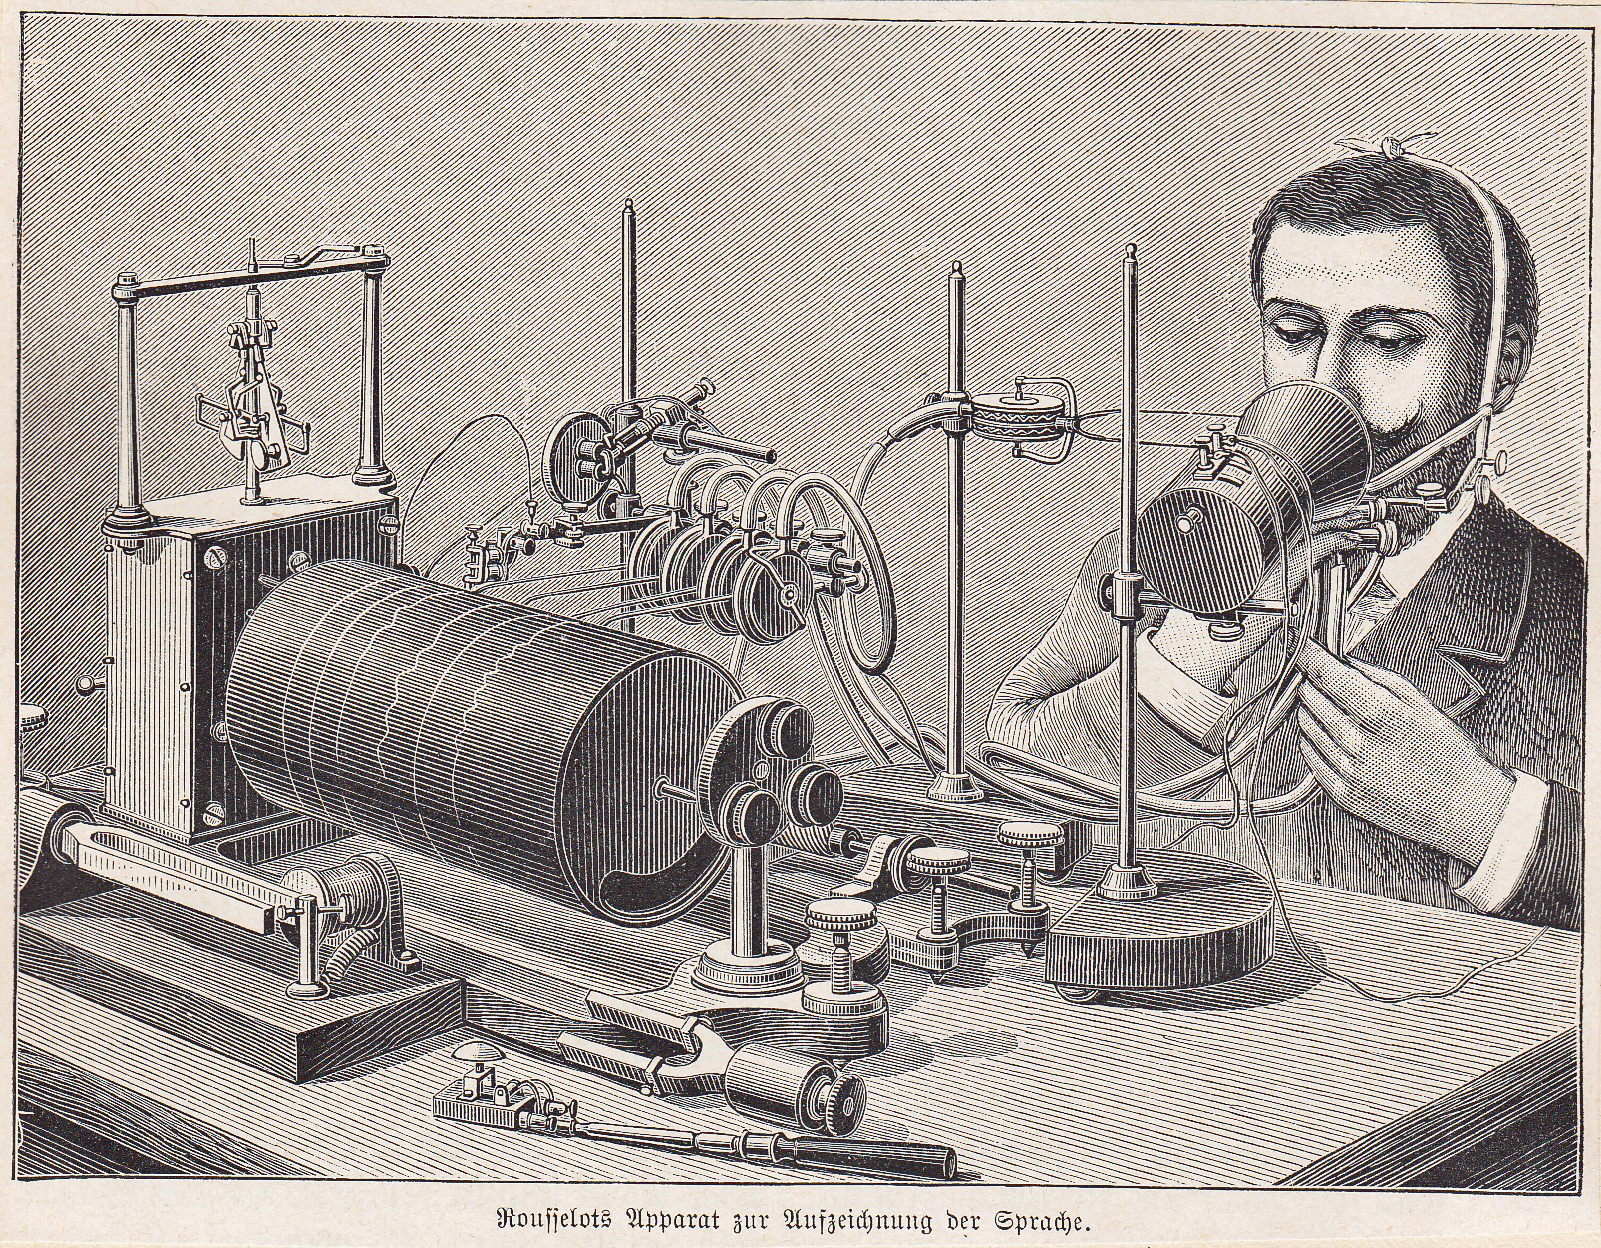
\includegraphics[scale=0.1]{material/04RousselotsApparatzurAufzeichnungderSprache}
		\caption{Rousselots Apparat zur Aufzeichnung der Sprache (Holzstich, um 1900). (https://de.wikipedia.org/wiki/Jean-Pierre$\_$Rousselot$\#$ /media/File:Rousselots$\_$Apparat$\_$zur$\_$Aufzeichnung$\_$der$\_$Sprache.jpg Stand: 09.12.16)
}
		%{material/04proband}
		%\caption{Proband \citep{Pompino95a}}
		%\label{Zeichen1}
	\end{figure}
	
\end{frame}


%%%%%%%%%%%%%%%%%%%%%%%%%%%%%%%%%%%%%%%%%%%%%%%%%%%%%%%%%%%%%%%%

\begin{frame}
\frametitle{Methodik}

	\begin{itemize}
		\item Der geschulte Ohrenphonetiker analysiert und beschreibt (\textbf{deskriptive Phonetik}) das Gehörte. Die analysierten Lautkategorien werden anschließend mit symbolischen Mitteln (dem Internationalen Phonetischen Alphabet -- IPA) dargestellt (\textbf{Symbolphonetik}).
		\item[]
		\item Phonetiker nehmen die ablaufenden physikalischen Vorgänge mittels spezieller Mess- oder Registriergeräte während des Sprechaktes als Signale auf (\textbf{Instrumental-} oder \textbf{Signalphonetik}).
	\end{itemize}
	
\end{frame}



%%%%%%%%%%%%%%%%%%%%%%%%%%%%%%%%%%%%%%%%%%%%%%%%%%%%%%%%%%%%%%%%

\begin{frame}
\frametitle{Methodik}

	\begin{itemize}
		\item Beispiele

			\ea Kiefer-, Lippen- und Zungenbewegungen mithilfe der elektrischen Muskelpotenziale
			\z
			
			\ea Luftdruckschwankungen, die das akustische Signal darstellen
			\z
			
			\ea Verlauf des intraoralen Luftdrucks
			\z
			
			\ea Veränderung der Durchblutung bestimmter Großhirnregionen bei der Verarbeitung von lautsprachlichen Reizen
			\z
			
	\end{itemize}
	
\end{frame}



%%%%%%%%%%%%%%%%%%%%%%%%%%%%%%%%%%%%%%%%%%%%%%%%%%%%%%%%%%%%%%%%

\begin{frame}
\frametitle{Methodik}

	\begin{itemize}
		\item Außerdem kann man den Zusammenhang zwischen bestimmten Signalausprägungen und der Wahrnehmung von Versuchspersonen untersuchen (\textbf{Experimentalphonetik} oder \textbf{perzeptive Phonetik}). Damit wird ein Zusammenhang zwischen der Instrumentalphonetik und der deskriptiven Phonetik erzeugt.

		\ea Bei Veränderung von einzelnen akustischen Parametern: Ab wann nimmt eine Versuchsperson ein \textipa{[ da ]} als \textipa{[ ta ]} wahr?
		\z

	\end{itemize}
	
\end{frame}



%%%%%%%%%%%%%%%%%%%%%%%%%%%%%%%%%%%%%%%%%%%%%%%%%%%%%%%%%%%%%%%%
%%%%%%%%%%%%%%%%%%%%%%%%%%%%%%%%%%%%%%%%%%%%%%%%%%%%%%%%%%%%%%%%
%
\section{Probleme der Phonetik}
\iftoggle{toc}{
\frame{
\begin{multicols}{2}
	\tableofcontents[currentsection]
\end{multicols}
}
}
%%%%%%%%%%%%%%%%%%%%%%%%%%%%%%%%%%%%%%%%%%%%%%%%%%%%%%%%%%%%%%%%%

\begin{frame}{Probleme der Phonetik}

	\begin{itemize}
		\item Schnelle Übermittlung der Laute:
		
		\begin{itemize}
			\item kurzer Satz (mit 50 Segmenten) \ras ung. 2 Sekunden
			\item[]
			\item d.\,h. bis zu 25 (sprachliche) Segmente pro Sekunde
			\item[]
			\item Nicht-sprachliche Segmente \ras ung. 7 bis 9 pro Sekunde
			\item[]
			\item[\ra] Hohe Geschwindigkeit bei der Äußerung eines Satzes macht aus einer sprachlichen Äußerung ein \textbf{Kontinuum}, in dem die Segmentierung der Laute besonders schwer ist.
		\end{itemize}
		
	\end{itemize}
	
\end{frame}


%%%%%%%%%%%%%%%%%%%%%%%%%%%%%%%%%%%%%%%%%%%%%%%%%%%%%%%%%%%%%%%

\begin{frame}
\frametitle{Probleme der Phonetik}

	\begin{figure}[H]
		\centering
		
		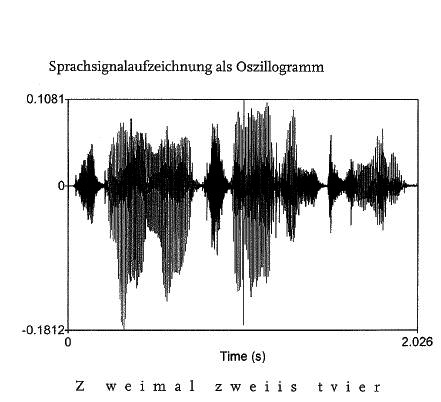
\includegraphics[scale=0.6]{material/04oszillogrammwiese}
		\caption{Oszillogramm \citep{WieseR11a}}
		%\label{Zeichen1}
	\end{figure}	
	
\end{frame}


%%%%%%%%%%%%%%%%%%%%%%%%%%%%%%%%%%%%%%%%%%%%%%%%%%%%%%%%%%%%%%%%

\begin{frame}
\frametitle{Probleme der Phonetik}

	\begin{itemize}
		\item Keine 1-zu-1-Korrespondenz zwischen Lauten und Verschriftlichung
		
		\begin{itemize}
			\item[]
			\item Ein Laut \ras mehrere Buchstaben

			\ea \textipa{[s]} \ras \ab{Smaragd}, \ab{groß}, \ab{essen}
			\z
			
			\item[]
			\item Eine Buchstabenfolge \ras unterschiedliche Laute

			\ea \ab{ch} \ras \ab{mich}, \ab{Buch}, \ab{sechs}, \ab{Charme}, \ab{Chip}
			\z

			\item[]
			\item[\ras] Schriftsystem mit 1-zu-1-Korrespondenz zwischen Lauten und (diakritischen) Zeichen: \textbf{IPA-Alphabet}
		\end{itemize}
		
	\end{itemize}
	
\end{frame}


%%%%%%%%%%%%%%%%%%%%%%%%%%%%%%%%%%%%%%%%%%%%%%%%%%%%%%%%%%%%%%%%
%%%%%%%%%%%%%%%%%%%%%%%%%%%%%%%%%%%%%%%%%%%%%%%%%%%%%%%%%%%%%%%%
%
\section{IPA-Alphabet}
\iftoggle{toc}{
\frame{
\begin{multicols}{2}
	\tableofcontents[currentsection]
\end{multicols}
}
}
%%%%%%%%%%%%%%%%%%%%%%%%%%%%%%%%%%%%%%%%%%%%%%%%%%%%%%%%%%%%%%%%

\begin{frame}{IPA-Alphabet}

	\begin{itemize}
		\item IPA = International Phonetic Association \ras IPA-Alphabet
		\item Seit dem 19. Jh. \ras Entwicklung von phonetischen Umschriftsystemen
		\item IPA-Alphabet ist das am weitesten verbreitete System.
		\item Alle Sprachlaute aller natürlichen Sprachen werden eindeutig dargestellt (phonetische Transkription).
		\item[]
		\item \textbf{Repräsentation der Phone} \ras in eckigen Klammern \gqq{\textipa{[ ]}}
		\item \textbf{Orthographische Repräsentation} \ras in spitzen Klammern \gqq{$\langle{} \rangle{}$}
		\item[]
		\item \textbf{LINK:} \href{http://internationalphoneticassociation.org}{Webseite der IPA}
		\item \textbf{LINK:} \href{http://phonetics.ucla.edu/course/chapter1/chapter1.html}{Alle Laute zum Testen}
	\end{itemize}
	
\end{frame}


%%%%%%%%%%%%%%%%%%%%%%%%%%%%%%%%%%%%%%%%%%%%%%%%%%%%%%%%%%%%%%%%

%\begin{frame}
%\frametitle{IPA-Alphabet}
%
%	\begin{figure}[H]
%		\centering
%		
%		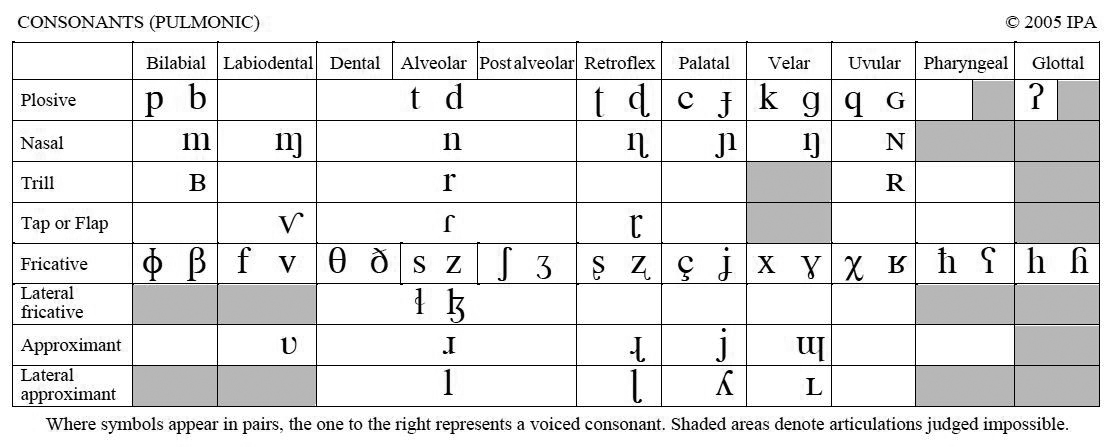
\includegraphics[scale=0.35]{material/04ipaconsonantpulmonic}
%		\caption{Konsonanten (Pulmonal)}
%		%\label{Zeichen1}
%	\end{figure}	
%	
%\end{frame}

%%%%%%%%%%%%%%%%%%%%%%%%%%%%%%%%%%%%%%%%%%%%%%%
\begin{frame}
\frametitle{IPA-Alphabet}
\begin{table}
\centering
\begin{adjustbox}{max width=\textwidth}
\begin{tabular}{|p{0.1\textwidth}|c|c|c|c|c|c|c|c|c|c|c|c|c|}
\hline
& \tiny{Bilabial} & \tiny{Labiodental} & \tiny{Dental} & \tiny{Alveolar} & \tiny{Postalveolar} & \tiny{Retroflex} & \tiny{Palatal} & \tiny{Velar} & \tiny{Uvular} & \multicolumn{2}{|c|}{\tiny{Pharyngal}} & \multicolumn{2}{|c|}{\tiny{Glottal}} \\
\hline
\tiny{Plosive} & \textipa{p b} & & \multicolumn{3}{|c|}{\textipa{t d}} & \textipa{\:d \:t} & \textipa{c \textbardotlessj} & \textipa{k g} & \textipa{q \textscg} &  & \cellcolor{lightgray} & \textipa{P} & \cellcolor{lightgray} \\
\hline
\tiny{Nasale} & \textipa{m} & \textipa{\textltailm} & \multicolumn{3}{|c|}{\textipa{n}} & \textipa{\textrtailn} & \textipa{\textltailn} & \textipa{\ng} & \textipa{\textscn} & \multicolumn{2}{|c|}{\cellcolor{lightgray}} & \multicolumn{2}{|c|}{\cellcolor{lightgray}} \\
\hline
\tiny{Vibranten} & \textipa{\textscb} & & \multicolumn{3}{|c|}{\textipa{r}} & & & \cellcolor{lightgray} & \textipa{\textscr} & \multicolumn{2}{|c|}{} & \multicolumn{2}{|c|}{\cellcolor{lightgray}} \\
\hline
\tiny{Taps/ Flaps} & & &  \multicolumn{3}{|c|}{\textipa{\textfishhookr}} &  \textipa{\textrtailr} & & \cellcolor{lightgray} & & \multicolumn{2}{|c|}{} & \multicolumn{2}{|c|}{\cellcolor{lightgray}} \\
\hline
\tiny{Frikative} & \textipa{\textphi \textbeta} & \textipa{f v} & \textipa{\texttheta \dh} & \textipa{s z} & \textipa{S Z} & \textipa{\:s \:z} & \textipa{\c{c} J} & \textipa{x G} & \textipa{X \textinvscr} & \multicolumn{2}{|c|}{\textipa{\textcrh \textrevglotstop}} & \multicolumn{2}{|c|}{\textipa{h \texthth}} \\
\hline
\tiny{Laterale Frikative} & \cellcolor{lightgray} & \cellcolor{lightgray} & \multicolumn{3}{|c|}{\textipa{\textbeltl \textlyoghlig}} & & & & &  \multicolumn{2}{|c|}{\cellcolor{lightgray}} & \multicolumn{2}{|c|}{\cellcolor{lightgray}} \\
\hline
\tiny{Approximanten} & & \textipa{\textscriptv} & \multicolumn{3}{|c|}{\textipa{\textturnr}} & \textipa{\:R} & \textipa{j} & \textipa{\textturnmrleg} & & \multicolumn{2}{|c|}{} & \multicolumn{2}{|c|}{\cellcolor{lightgray}} \\
\hline
\tiny{Laterale Approximanten} & \cellcolor{lightgray} & \cellcolor{lightgray} & \multicolumn{3}{|c|}{\textipa{l}} & \textipa{\:l} & \textipa{\textturny} & \textipa{\textscl} & & \multicolumn{2}{|c|}{\cellcolor{lightgray}} & \multicolumn{2}{|c|}{\cellcolor{lightgray}} \\
\hline
\end{tabular}
\end{adjustbox}
\caption{Pulmonische Konsonanten, IPA (2005). Bei Paaren ist der rechte Konsonant stimmhaft. Graue Flächen gelten als artikulatorisch unmöglich. 
	 %https://www.internationalphoneticassociation.org/sites/default/files/pulmonic.gif Stand: 09.12.16
 } 
\end{table}

\end{frame}

%%%%%%%%%%%%%%%%%%%%%%%%%%%%%%%%%%%%%%%%%%%%%%%%%%%%%%%%%%%%%%%%

\begin{frame}
\frametitle{IPA-Alphabet}

	\begin{figure}[H]
		\centering
		
		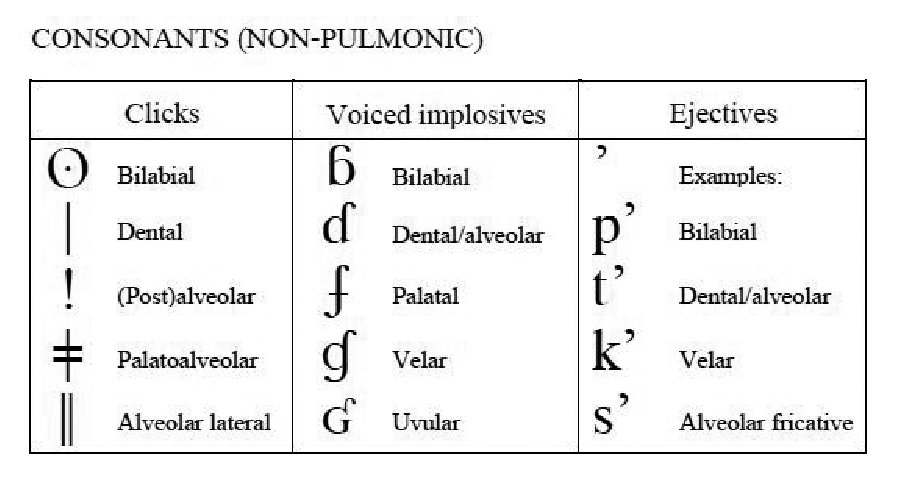
\includegraphics[scale=0.45]{material/04ipaconsonantnonpulmonic}
		\caption{Konsonanten (Nicht Pulmonal)}
		%\label{Zeichen1}
	\end{figure}
	
	\begin{itemize}
		\item \textbf{VIDEO:} \href{run:material/04namaclicks.mp4}{!Nama Clicks}
	\end{itemize}
			
\end{frame}



%%%%%%%%%%%%%%%%%%%%%%%%%%%%%%%%%%%%%%%%%%%%%%%%%%%%%%%%%%%%%%%%%%%

\begin{frame}
\frametitle{IPA-Alphabet}

	\begin{figure}[H]
		\centering
		
		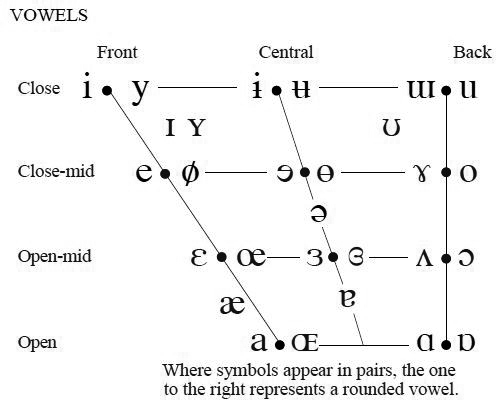
\includegraphics[scale=0.45]{material/04ipavowel}
		\caption{Vokale}
		%\label{Zeichen1}
	\end{figure}
	
\end{frame}


%%%%%%%%%%%%%%%%%%%%%%%%%%%%%%%%%%%%%%%%%%%%%%%%%%%%%%%%%%%%%%%%

\begin{frame}
\frametitle{IPA-Alphabet}

	\begin{figure}[H]
		\centering
		
		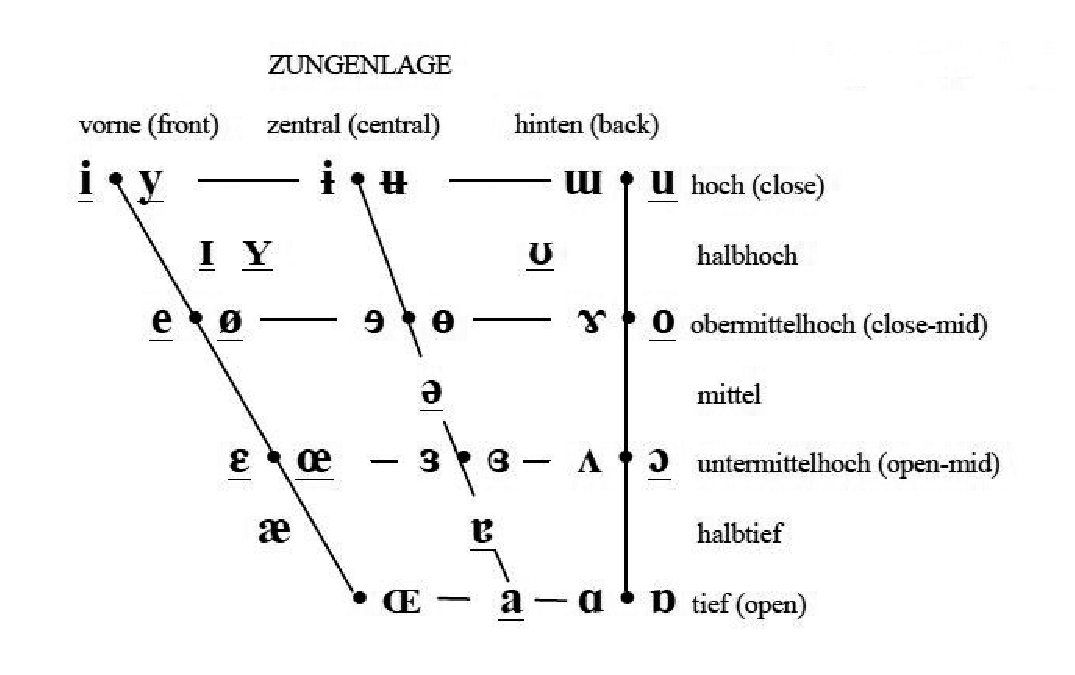
\includegraphics[scale=0.5]{material/04ipatabellerepp11vokalviereck}
		\caption{Vokale für das Deutsche}
		%\label{Zeichen1}
	\end{figure}
	
\end{frame}


%%%%%%%%%%%%%%%%%%%%%%%%%%%%%%%%%%%%%%%%%%%%%%%%%%%%%%%%%%%%%%%%

\begin{frame}
\frametitle{IPA-Alphabet}

	\begin{figure}[H]
		\centering
		
		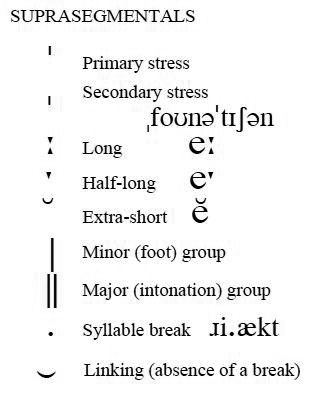
\includegraphics[scale=0.5]{material/04ipasuprasegmental}
		\caption{Suprasegmentalia}
		%\label{Zeichen1}
	\end{figure}
	
\end{frame}


%%%%%%%%%%%%%%%%%%%%%%%%%%%%%%%%%%%%%%%%%%%%%%%%%%%%%%%%%%%%%%%%
%%%%%%%%%%%%%%%%%%%%%%%%%%%%%%%%%%%%%%%%%%%%%%%%%%%%%%%%%%%%%%%%
%
\section{Artikulatorische Phonetik}
\iftoggle{toc}{
\frame{
\begin{multicols}{2}
	\tableofcontents[currentsection]
\end{multicols}
}
}
%%%%%%%%%%%%%%%%%%%%%%%%%%%%%%%%%%%%%%%%%%%%%%%%%%%%%%%%%%%%%%%%

\begin{frame}{Artikulatorische Phonetik}

	\begin{itemize}
		\item Mehrere Körperteile sind für Erzeugung von Schall nötig:
		
		\begin{itemize}
			\item[]
			\item \textbf{Initiator}: die Lunge \ras (Atmung) erzeugt Luftstrom
			\item[]
			\item \textbf{Generator}: der Kehlkopf (Larynx) mit den Stimmbändern \ras Luftstrom wird in Schwingung versetzt (Phonation)
		\end{itemize}
		
		\begin{itemize}
			\item[] Frequenz: Häufigkeit mit der die Stimmlippen schwingen bestimmt die Tonhöhe (in Hz).
			\item[]

			\ea Bei Frauen ung. 230 Hz, bei Männern 120 Hz und bei Säuglingen 400 Hz
			\z

		\end{itemize}
		
		\begin{itemize}
			\item[] \textbf{VIDEO:} \href{run:material/04TransNasalEndoscopy.mp4}{Trans-Nasal Endoscopy}
		\end{itemize}
		
	\end{itemize}
	
\end{frame}


%%%%%%%%%%%%%%%%%%%%%%%%%%%%%%%%%%%%%%%%%%%%%%%%%%%%%%%%%%%%%%%%

\begin{frame}
\frametitle{Artikulatorische Phonetik}

	\begin{itemize}
		\item \textbf{Modifikator}: Rachen-, Mund- und Nasenraum mit den verschiedenen Sprechwerkzeugen (Zunge, Lippen, weicher Gaumen) \ras unterschiedliche Stellung der Artikulationsorgane verändert den Rohschall des Kehlkopfs zu den wohlunterschiedenen Lauten (Artikulation im engeren Sinne).
	\end{itemize}
	
\end{frame}



%%%%%%%%%%%%%%%%%%%%%%%%%%%%%%%%%%%%%%%%%%%%%%%%%%%%%%%%%%%%%%%%%%%%%%%%%%%%%%%%%%%%%%%%%%%%%%%%%%%%%%%%%%%%%%%%%%%%%%%%%%%%%%%%
%
\subsection{Konsonanten}
%\frame{
%\begin{multicols}{2}
%	\tableofcontents[currentsection]
%\end{multicols}
%}
%%%%%%%%%%%%%%%%%%%%%%%%%%%%%%%%%%%%%%%%%%%%%%%%%%%%%%%%%%%%%%%%

\begin{frame}{Konsonanten}

	\begin{itemize}
		\item Konsonanten \ras Mitlaute
		\item[]
		\item Die Artikulationsorgane bilden eine \textbf{geräuschverursachende Enge} oder einen Verschluss im Ansatzrohr, d.\,h. die Luft wird oberhalb der Stimmritze (Glottis) zwischen den Stimmbändern behindert.
	\end{itemize}
	
\end{frame}


%%%%%%%%%%%%%%%%%%%%%%%%%%%%%%%%%%%%%%%%%%%%%%%%%%%%%%%%%%%%%%%%

\begin{frame}
\frametitle{Konsonanten}

	\begin{figure}[H]
		\centering
		
		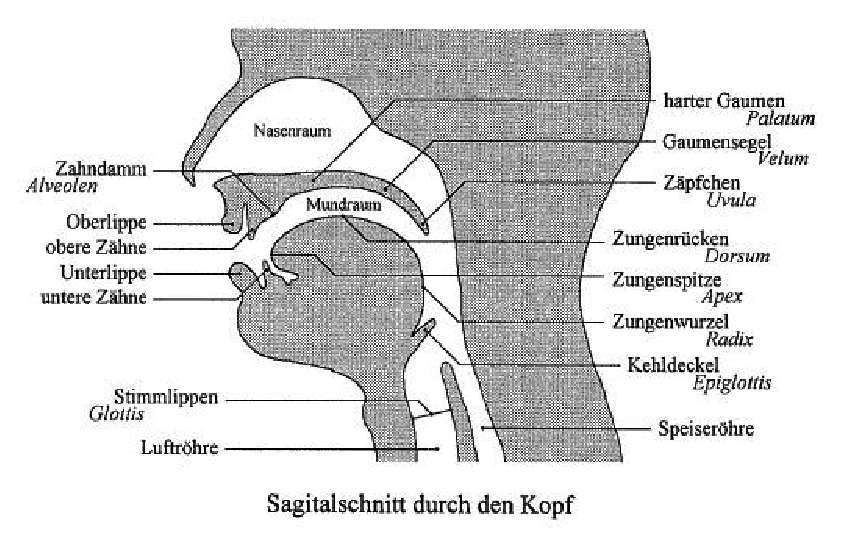
\includegraphics[scale=0.65]{material/04sagitalschnittaltmann}
		\caption{Sagitalschnitt \citep{Altmann&Co07a}}
		%\label{Zeichen1}
	\end{figure}
	
\end{frame}



%%%%%%%%%%%%%%%%%%%%%%%%%%%%%%%%%%%%%%%%%%%%%%%%%%%%%%%%%%%%%%%%
%%%%%%%%%%%%%%%%%%%%%%%%%%%%%%%%%%%%%%%%%%%%%%%%%%%%%%%%%%%%%%%%
%
\subsubsection{Konsonantenklassifikation}
%
%%%%%%%%%%%%%%%%%%%%%%%%%%%%%%%%%%%%%%%%%%%%%%%%%%%%%%%%%%%%%%%%

\begin{frame}{Konsonantenklassifikation}

	\begin{itemize}
		\item \textbf{Stimmbeteiligung} (Stimmhaftigkeit): Schwingungszustand der Stimmbänder
		
		\begin{itemize}
			\item[]
			\item \textbf{stimmhaft} \ras eng beieinander stehende Stimmbänder
			\item[]
			\item \textbf{stimmlos} \ras weit auseinander stehende Stimmbänder

			\ea \textipa{[ p ]} vs. \textipa{[ b ]}
			\z

			\item[]
			\item \textbf{Aspiration} (Behauchung): Glottis während der Verschlussphase ist weit gespreizt und schwingt mit.

			\ea \textipa{[ \super h ]}
			\z

		\end{itemize}

	\end{itemize}
	
\end{frame}



%%%%%%%%%%%%%%%%%%%%%%%%%%%%%%%%%%%%%%%%%%%%%%%%%%%%%%%%%%%%%%%%

\begin{frame}
\frametitle{Konsonantenklassifikation}

\begin{itemize}
		\item \textbf{ÜB:} Welche der folgenden Laute sind stimmhaft und welche stimmlos?

		\ea \textipa{[ d, z, f, v, g, k, P ]}
		\z
		
\end{itemize}

\end{frame}


%%%%%%%%%%%%%%%%%%%%%%%%%%%%%%%%%%%%%%%%%%%%%%%%%%%%%

\begin{frame}
\frametitle{Lösung}

\begin{itemize}
\item stimmhaft: \textipa{[ d, z, v, g ]}
\item[]
\item stimmlos: \textipa{[ f, k, P ]}
\end{itemize}
\end{frame}

%%%%%%%%%%%%%%%%%%%%%%%%%%%%%%%%%%%%%%%%%%%%%%%%%%%%%%%%%%%%%%%%

\begin{frame}
\frametitle{Konsonantenklassifikation}

	\begin{itemize}
		\item \textbf{Stellung des Gaumensegels} (des weichen Gaumens):
		
		\begin{itemize}
			\item[]
			\item Nasale Laute (\zB \textipa{ [ m , n ]}) \ras Senkung des weichen Gaumens (Velum)
			\item[]
			\item Orale Laute (\zB \textipa{ [ f , a ]}) \ras bei gehobenem Velum
		\end{itemize}
		
		\item[]
		\item \textbf{LINK:} \href{http://smu-facweb.smu.ca/~s0949176/sammy/}{Interactive Sagittal Section}
	\end{itemize}
	
\end{frame}


%%%%%%%%%%%%%%%%%%%%%%%%%%%%%%%%%%%%%%%%%%%%%%%%%%%%%%%%%%%%%%%%

\begin{frame}
\frametitle{Konsonantenklassifikation}

	\begin{itemize}
		\item \textbf{Artikulationsort} im Vokaltrakt: Ort, an dem die Luft behindert wird. Man unterscheidet darunter die nicht-beweglichen von den beweglichen Artikulatoren.

		\item[]
		\item \textbf{Nicht-bewegliche} Artikulatoren (passiver Artikulator, Artikulationsort im engeren Sinne):
			
		\begin{itemize}
			\item die oberen Zähne \ras dental
			\item[]
			\item die Alveolen (Knochendamm hinter den oberen Zähne) \ras alveolar
			\item[]
			\item der harte Gaumen (Palatum) \ras palatal
		\end{itemize}
		
	\end{itemize}
	
\end{frame}


%%%%%%%%%%%%%%%%%%%%%%%%%%%%%%%%%%%%%%%%%%%%%%%%%%%%%%%%%%%%%%%%

\begin{frame}
\frametitle{Konsonantenlassifikation}

\begin{itemize}
	\item \textbf{Bewegliche} Artikulatoren (aktiver Artikulator, Artikulationsorgan):
			
	\begin{itemize}
		\item[]
		\item weicher Gaumen (Velum) \ras velar
		\item[]
		\item das Zäpfchen (Uvula) \ras uvular
		\item[]
		\item Lippen \ras labial
		\item[]
		\item Unterkiefer
		\item[]
		\item Zunge
	\end{itemize}

\end{itemize}

\end{frame}


%%%%%%%%%%%%%%%%%%%%%%%%%%%%%%%%%%%%%%%%%%%%%%%%%%%%%%%%%%%%%%

\begin{frame}
\frametitle{Konsonantenklassifikation}

	\begin{itemize}
		\item \textbf{EXTRA-INFORMATION:}
		
		\begin{itemize}
			\item[]
			\item Bei der Artikulation mit der Zunge bildet man Untergruppen nach dem beteiligten Zungenteil:
			
			\begin{itemize}
				\item[]
				\item \textbf{koronal}: mit dem vorderen Teil der Zunge\\
				\ras \textbf{apikal}: mit der Zungenspitze\\
				\ras \textbf{laminal}: mit dem Zungenblatt (mittlerer Teil der Zunge)

				\ea \textipa{[ t, d, l, n, s, z, S, Z ]}
				\z

				\item \textbf{dorsal}: mit dem hinteren Teil der Zunge

				\ea \textipa{[ \c{c}, j, g, k, x, N, \textscr , K ]}
				\z

			\end{itemize}
						 
		\end{itemize}
		
		\item[]
		\item \textbf{LINK:} \href{http://smu-facweb.smu.ca/~s0949176/sammy/}{Interactive Sagittal Section}
	\end{itemize}
	
\end{frame}


%%%%%%%%%%%%%%%%%%%%%%%%%%%%%%%%%%%%%%%%%%%%%%%%%%%%%%%%%%%%%%%%

\begin{frame}
\frametitle{Konsonantenklassifikation}

	\begin{itemize}
		\item \textbf{Artikulationsart} (Artikulationsmodus): Art der Behinderung des Luftstroms durch die Artikulationsorgane

			\item[]
			\item \textbf{Plosive} (Verschlusslaute, Explosivlaute, stops): Totaler oraler Verschluss mit anschließender plötzlicher Lösung des Verschlusses\\
	Das Velum bleibt dabei in angehobener Position, so dass die Luft durch den Mundraum strömt.

			\ea \textipa{[ p, b, t, d, k, g, P ]}
			\z
			
			\begin{itemize}
				\item Der \textbf{Glottalverschluss} (Knacklaut) \textipa{[ P ]} entsteht durch plötzliches Öffnen der Stimmritze und kommt im Deutschen vor anlautendem Vokal eines Wortes und vor anlautendem Vokal in einer betonten Silbe vor.
			\end{itemize}
		
	\end{itemize}
	
\end{frame}


%%%%%%%%%%%%%%%%%%%%%%%%%%%%%%%%%%%%%%%%%%%%%%%%%%%%%%%%%%%%%%%%

\begin{frame}
\frametitle{Konsonantenklassifikation}

		\begin{itemize}
			\item \textbf{Frikative} (Reibelaute, Spiranten): Verengung zweier Sprechorgane, Luftstrom strömt durch die Verengung, es entsteht ein Reibegeräusch.

			\ea \textipa{[ f, v, s, z, S, Z, \c{c}, x, h, K ]}
			\z
			
			\begin{itemize}
				\item \textbf{Sibilanten} (Zischlaut): Unterklasse der Frikative mit intensivem, hochfrequentem Geräuschanteil.

				\ea \textipa{[ s, z, S ]}
				\z

		\end{itemize}
		
	\end{itemize}
	
\end{frame}


%%%%%%%%%%%%%%%%%%%%%%%%%%%%%%%%%%%%%%%%%%%%%%%%%%%%%%%%%%%%%%%%

\begin{frame}
\frametitle{Konsonantenklassifikation}

		\begin{itemize}
			\item \textbf{Affrikaten}: Plosive, die in Frikative übergehen, wobei die Verschlussphase und die Frikativphase dieselbe (oder annähernd dieselbe) Artikulationsstelle haben; d.\,h. sie sind \textbf{homorgan}.

			\ea \textipa{[ \t{pf} , \t{ts} , \t{tS} , \t{dZ} ]}
			\z

			\begin{itemize}
				\item Per Definitionem gehören der plosive und der frikative Laut einer Affrikaten \textbf{zum selben Morphem} (die kleinste Bedeutungs-tragende Einheit). Daraus ergibt sich:

				\ea \textipa{[ \t{ts} ]} in \ab{Blitz} \ras Affrikate
				\z
				
				\ea \textipa{[ \t{ts} ]} in \ab{Monats} \ras keine Affrikate
				\z

			\end{itemize}
		
		\item[]
		\item Plosive, Frikative und Affrikaten \ras \textbf{Obstruenten}
	\end{itemize}
	
\end{frame}


%%%%%%%%%%%%%%%%%%%%%%%%%%%%%%%%%%%%%%%%%%%%%%%%%%%%%%%%%%%%%%%%

\begin{frame}
\frametitle{Konsonantenklassifikation}

		\begin{itemize}
			\item \textbf{Vibranten} (trills): schnelle Folge oraler Verschlüsse
			\begin{itemize}
				\item[]
				\item Artikulationsstellen für Vibranten sehr eingeschränkt: nur bilabial, alveolar oder uvular
				\item[]
				\item Der alveolare Vibrant \textipa{[ r ]} (das sog. Zungenspitzen-R) kommt in vielen süddeutschen Varietäten vor.
				\item[]
				\item Der uvulare Vibrant \textipa{[ \textscr ]} (das gerollte Zäpfchen-R) ist eine häufige Realisierung des Deutschen \ab{r}.
			\end{itemize}
			 
	\end{itemize}
	
\end{frame}


%%%%%%%%%%%%%%%%%%%%%%%%%%%%%%%%%%%%%%%%%%%%%%%%%%%%%%%%%%%%%%%%

\begin{frame}
\frametitle{Konsonantenklassifikation}

		\begin{itemize}
			\item \textbf{Approximanten} (Öffnungslaute): Enge im Ansatzrohr (wie Frikative)\\
			Bei Approximanten gibt es nicht so eine große Nähe zwischen Artikulator und Artikulationsstelle \ras kein Reibegeräusch
			\item[]
			\item[] Zwei Unterklassen:
			
			\begin{itemize}
				\item[]
				\item \textbf{Laterale}: Verschluss in der Mundhöhlenmitte, Luft entweicht seitlich [~\textipa{l}~]
				\item[]
				\item \textbf{Gleitlaute} (zentral): zentrale Verengung aber weiter als bei Frikativen [~\textipa{w}~].\\
				(Manchmal wird [~\textipa{j}~] auch zu den Gleitlauten gezählt, da die Verengung weiter als bei anderen Frikativen ist, dies ist jedoch strittig!)
			\end{itemize}
			
		\end{itemize}	

\end{frame}


%%%%%%%%%%%%%%%%%%%%%%%%%%%%%%%%%%%%%%%%%%%%%%%%%%%%%%%%%%%%%%%%

\begin{frame}
\frametitle{Konsonantenklassifikation}

		\begin{itemize}
			\item \textbf{Nasale}: totaler oraler Verschluss (wie Plosive). Luft entweicht durch die Nase durch Senken des Velums\\
			\item[] Im Deutschen kommen 3 Nasale vor: \textipa{[ m, n, N ]}

		\item[]
		\item Vibranten, Approximanten (Laterale und Gleitlaute), Nasale und Vokale (auch die hier nicht behandelten \gqq{geschlagenen Laute} wie das span. \textipa{[ R ]}) gehören zur Gruppe der \textbf{Sonoranten}, da die Luft bei denen ungehindert ausströmen kann. Sonoranten sind \textbf{immer} stimmhaft!
		\item[]
		\item Die Klasse der l-Laute und r-Laute werden auch zu den sog. \textbf{Liquiden} zusammengefasst (im Dt. \textipa{[ l, r, \textscr ]})
	\end{itemize}
	
\end{frame}


%%%%%%%%%%%%%%%%%%%%%%%%%%%%%%%%%%%%%%%%%%%%%%%%%%%%%%%%%%%%%%%%

\begin{frame}
\frametitle{Konsonantenklassifikation}

	\begin{itemize}
		\item Für die Differenzierung der deutschen Konsonanten sind hauptsächlich 3 Merkmale wichtig:
		
		\begin{itemize}
			\item[]
			\item Stimmbeteiligung
			\item Artikulationsort
			\item Artikulationsart
		\end{itemize}
		
		\item[]
		\item \textbf{ÜB:} Beschreiben Sie die Konsonanten in den folgenden Wörtern und geben Sie die entsprechenden phonetischen Symbole an:
		\item[] Busch, malen, Maus, Achtung, Genie, zirpen, wichtig, Wald
	\end{itemize}
	
\end{frame}


%%%%%%%%%%%%%%%%%%%%%%%%%%%%%%%%%%%%%%%%%%%%%%%%%%%%%%%%%%%%%%%%
%
\subsection{Vokale}
\iftoggle{toc}{
\frame{
\begin{multicols}{2}
	\tableofcontents[currentsection]
\end{multicols}
}
}
%%%%%%%%%%%%%%%%%%%%%%%%%%%%%%%%%%%%%%%%%%%%%%%%%%%%%%%%%%%%%%%%

\begin{frame}{Vokale}

	\begin{itemize}
		\item \textbf{Vokale} (Selbstlaute) sind Laute, bei deren Artikulation die Luft ungehindert durch den Mundraum strömen kann (deswegen gehören sie zu den Sonoranten)
		\item[]
		\item Vokale sind \idR immer stimmhaft.
		\item[]
		\item Es ist umstritten, ob der sog. Schwa-Laut im Dt. \textipa{[ @ ]} stimmhaft ist, auch im Japanischen soll es stimmlose Vokale geben
	\end{itemize}
	
\end{frame}


%%%%%%%%%%%%%%%%%%%%%%%%%%%%%%%%%%%%%%%%%%%%%%%%%%%%%%%%%%%%%%%%
%%%%%%%%%%%%%%%%%%%%%%%%%%%%%%%%%%%%%%%%%%%%%%%%%%%%%%%%%%%%%%%%
%
\subsubsection{Vokalklassifikation}
%
%%%%%%%%%%%%%%%%%%%%%%%%%%%%%%%%%%%%%%%%%%%%%%%%%%%%%%%%%%%%%%%%

\begin{frame}{Vokalklassifikation}

	\begin{itemize}
		\item \textbf{Zungenhöhe} (Vokalhöhe): Grad der Zungenhebung in Richtung Gaumen

		\ea hoch: \textipa{[ i: ]}, mittel: \textipa{[ o: ]}, tief: \textipa{[ a: ]} bzw. geschlossen, halboffen, offen
		\z

		\item[]
		\item \textbf{Zungenlage} (Vokaltiefe): angehobener Teil der Zunge

		\ea vorne: \textipa{[ i: ]}, zentral: \textipa{[ a: ]}, hinten: \textipa{[ u: ]}
		\z

	\end{itemize}
	
\end{frame}


%%%%%%%%%%%%%%%%%%%%%%%%%%%%%%%%%%%%%%%%%%%%%%%%%%%%%%%%%%%%%%%%

\begin{frame}
\frametitle{Vokalklassifikation}

	\begin{itemize}
		\item \textbf{Lippenrundung}: Art der Lippenöffnung

		\ea gerundet: \textipa{[ o: ]}, ungerundet: \textipa{[ i: ]}
		\z

		\item[]
		\item\textbf{ÜB:} Lesen Sie die folgenden Wörter erst mit gerundeten danach mit gespreizten Lippen:
		\item[] Bühne, rühmen, Dünen, Stiele, Trieb, Möhre, Herd, Hefe
	\end{itemize}
	
\end{frame}


%%%%%%%%%%%%%%%%%%%%%%%%%%%%%%%%%%%%%%%%%%%%%%%%%%%%%%%%%%%%%%%%

\begin{frame}
\frametitle{Vokalklassifikation}

	\begin{itemize}
		\item \textbf{Gespanntheit} vs. Ungespanntheit der Muskeln (Länge, Vokalquantität):
		
		\begin{itemize}
			\item[]
			\item Definition 1: \textipa{[ i:, y:, u:, o: ]} \textbf{mehr Muskelspannung} als \textipa{[ I, Y, \textupsilon , O ]}\\
			(von der experimentellen Phonetik weder bestätigt noch widerlegt)
			\item[]
			\item Definition 2: mit vorverlagerter Zungenwurzel
			\item[]
			\item I.\;d.\textscr . alle tiefen Vokale \ras ungespannt (strittig!)
			\item langer tiefer Vokal \textipa{[ a: ]} \ras gespannt(?)
		\end{itemize}
		
	\end{itemize}
	
\end{frame}


%%%%%%%%%%%%%%%%%%%%%%%%%%%%%%%%%%%%%%%%%%%%%%%%%%%%%%%%%%%%%%%%

\begin{frame}
\frametitle{Vokalklassifikation}

	\begin{itemize}
	
		\item Im Deutschen: Korrelation der Gespanntheit mit der Länge.

		\ea \textipa{[ m i: t @ ]} vs. \textipa{[ m I t @ ]}
		\z

		\item In Lehnwörtern findet man auch kurze gespannte Vokale

		\ea \textipa{[ P i . d e: ]}
		\z
		
\vspace{1em}
		
		\item \textbf{Stellung des Gaumensegels}:
		
		\begin{itemize}
			\item oral
			\item nasal
			\item[]
			\item Nasalvokale kommen im Dt. nur in Lehnwörtern vor.

			\ea \textipa{[ \~a, \~o, \~E, \~\oe ]}
			\z
		
		\end{itemize}
		
	\end{itemize}
	
\end{frame}


%%%%%%%%%%%%%%%%%%%%%%%%%%%%%%%%%%%%%%%%%%%%%%%%%%%%%%%%%%%%%%%%

\begin{frame}
\frametitle{Vokalklassifikation}

	\begin{itemize}
		\item Für die Differenzierung der deutschen nativen Vokale sind hauptsächlich 4 Merkmale wichtig:
		
		\begin{itemize}
			\item[]
			\item Zungenhöhe
			\item[]
			\item Zungenlage
			\item[]
			\item Lippenrundung
			\item[]
			\item Gespanntheit (bzw. Länge)
		\end{itemize}
		
	\end{itemize}
	
\end{frame}


%%%%%%%%%%%%%%%%%%%%%%%%%%%%%%%%%%%%%%%%%%%%%%%%%%%%%%%%%%%%%%%%
%%%%%%%%%%%%%%%%%%%%%%%%%%%%%%%%%%%%%%%%%%%%%%%%%%%%%%%%%%%%%%%%
%
\subsubsection{Vokalviereck}
%\frame{
%\begin{multicols}{2}
%	\tableofcontents[currentsection]
%\end{multicols}
%}
%%%%%%%%%%%%%%%%%%%%%%%%%%%%%%%%%%%%%%%%%%%%%%%%%%%%%%%%%%%%%%%%

\begin{frame}{Vokalviereck}

	\begin{itemize}
		\item Für eine bessere Darstellung wurden die Vokale (von Daniel Jones 1920) in das sog. Vokalviereck angeordnet, welches eine stilisierte Version des Vokalraums darstellt.
	\end{itemize}

	\begin{figure}[H]
		\centering
		
		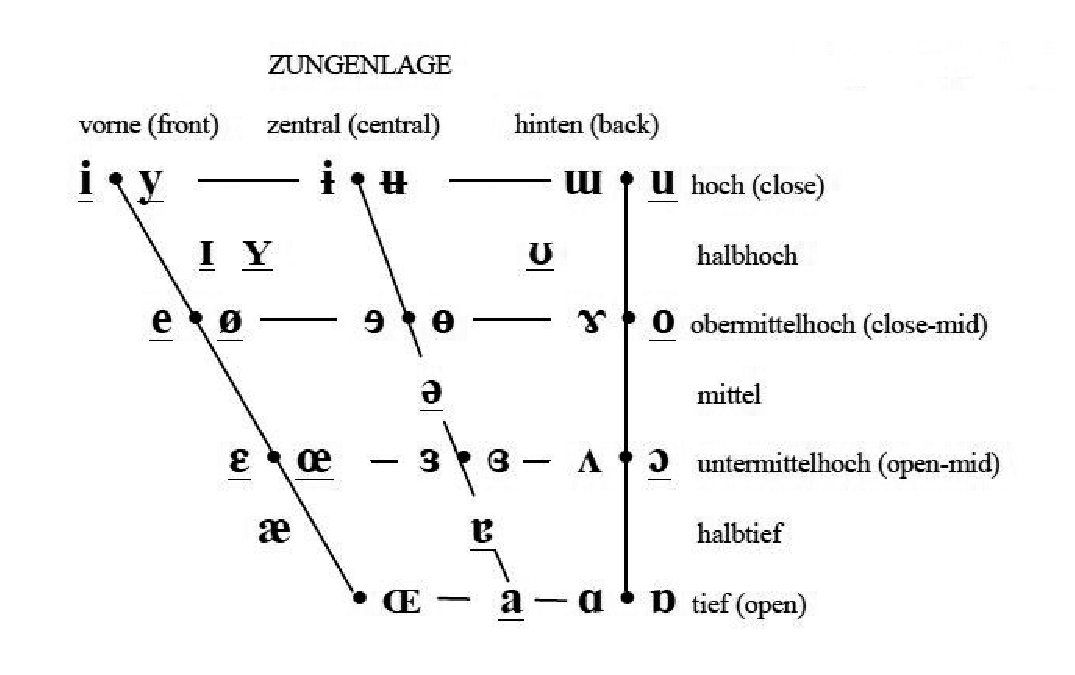
\includegraphics[scale=0.45]{material/04ipatabellerepp11vokalviereck}
		\caption{Vokalviereck \citep{Repp&Co12a}}
		%\label{Zeichen1}
	\end{figure}	
	
\end{frame}


%%%%%%%%%%%%%%%%%%%%%%%%%%%%%%%%%%%%%%%%%%%%%%%%%%%%%%%%%%%%%%%%
%%%%%%%%%%%%%%%%%%%%%%%%%%%%%%%%%%%%%%%%%%%%%%%%%%%%%%%%%%%%%%%%
%
\subsubsection{Monophthong, Diphthong, Triphthong}
%\frame{
%\begin{multicols}{2}
%	\tableofcontents[currentsection]
%\end{multicols}
%}
%%%%%%%%%%%%%%%%%%%%%%%%%%%%%%%%%%%%%%%%%%%%%%%%%%%%%%%%%%%%%%%%

\begin{frame}{Monophthong, Diphthong, Triphthong}

\begin{itemize}
	\item \textbf{Monophthong}

	\begin{itemize}		
		\item einzelner (langer oder kurzer) Vokal
		\item[]
	\end{itemize}
	
	\item \textbf{Diphthong} (Zwielaut, Doppellaut)
	
	\begin{itemize}		
		\item Abfolge von zwei Vokalen
		\item[]
		\item Beide Einheiten haben zusammen die gleiche Dauer wie ein einzelner langer Vokal
		\item[]
		\item Beide Vokale gehören zur selben Silbe (im Silbenkern)
		\item[]
		\item Zunge gleitet bei der Artikulation von einer Stellung in eine andere
		\item[]
		\item Laut ändert kontinuierlich seine Qualität
	\end{itemize}
	
\end{itemize}	

\end{frame}


%%%%%%%%%%%%%%%%%%%%%%%%%%%%%%%%%%%%%%%%%%%%%%%%%%%%%%%%%%%%%%%%

\begin{frame}
\frametitle{Monophthong, Diphthong, Triphthong}

	\begin{itemize}
		\item \textbf{Unterklassen} der Diphthonge:
		
		\begin{itemize}
			\item[]
			\item \textbf{fallende} (oder schließende) Diphthonge (echte deutsche Diphthonge)

			\ea \textipa{[ \t{aI} , \t{aU} , \t{OI} ]} oder \textipa{[ a\textsubarch{I} , a\textsubarch{U} , O\textsubarch{I} ]}
			\z

			\item[]
			\item \textbf{steigende} (oder öffnende) Diphthonge\\

			\ea Im Bayrischen: \textipa{[ \t{Ia} , \t{Ua} ]} oder \textipa{[ \textsubarch{I}a , \textsubarch{\textupsilon}a ]} (in \ab{liap} und \ab{guat})
			\z
			
			\ea In Fremdwörtern: \abe{Span\textit{ie}n}, \abe{Rit\textit{ua}l}, \abe{Stud\textit{iu}m}
			\z
			
			\item fallend vs. steigend \ras akustisch-auditiv
			\item schließend vs. öffnend \ras artikulatorisch
		\end{itemize}
		
	\end{itemize}
	
\end{frame}


%%%%%%%%%%%%%%%%%%%%%%%%%%%%%%%%%%%%%%%%%%%%%%%%%%%%%%%%%%%%%%%%

\begin{frame}
\frametitle{Monophthong, Diphthong, Triphthong}

\begin{itemize}
	\item[]
		
	\begin{itemize}
		\item \textbf{zentralisierende} Diphthonge (durch R-Vokalisierung \ras keine Phoneme)

		\ea \textipa{[ \t{i5} , \t{I5} , \t{e5} , \t{u5} , \t{y5} , \t{Y5} , \t{\o5} , \t{U5} , \t{o5} ]} in \abu{hier, Birke, mehr, stur, für, mürrisch, stör, knurr, Ohr}
		\z
		
	\end{itemize}

						 		
\end{itemize}
	
\end{frame}


%%%%%%%%%%%%%%%%%%%%%%%%%%%%%%%%%%%%%%%%%%%%%%%%%%%%%%%%%%%%%%%%

\begin{frame}
\frametitle{Monophthong, Diphthong, Triphthong}

\begin{itemize}
	\item \textbf{Triphthong} (Dreilaut)
	
	\begin{itemize}
		\item Abfolge von drei Vokalen im Silbenkern (?)
		\item[]
		\item Anzahl der Silben \ras unsicher
		\item[]
		\item \textbf{linear steigende}
		\item[]
		\item \textbf{linear fallende}
		\item[]
		\item mit \textbf{Umkehrpunkt}
	\end{itemize}
	
	\ea \textipa{[ \t{aI5} , \t{OI5}, \t{aU5} ]} in \ab{Eier, Steuer, Bauer}
	\z
	
\end{itemize}	

\end{frame}

	
	
%%%%%%%%%%%%%%%%%%%%%%%%%%%%%%%%%%%%%%%%%%%%%%%%%%%%%%%%%%%%%%%%
%%%%%%%%%%%%%%%%%%%%%%%%%%%%%%%%%%%%%%%%%%%%%%%%%%%%%%%%%%%%%%%%
%
\section{Übungen}
\iftoggle{toc}{
\frame{
\begin{multicols}{2}
\frametitle{~}
	\tableofcontents[currentsection]
\end{multicols}
}
}
%%%%%%%%%%%%%%%%%%%%%%%%%%%%%%%%%%%%%%%%%%%%%%%%%%%%%%%%%%%%%%%%

\begin{frame}
\frametitle{Übungen}

\begin{itemize}
	\item \textbf{ÜB:} Bilden die folgenden Vokalabfolgen Diphthonge?
		\item[] Zeit, naiv, Haus
\end{itemize}

\end{frame}


%%%%%%%%%%%%%%%%%%%%%%%%%%%%%%%%%%%%%%%%%%%%%%%%%%%%%%%%%%%%%%%%

\begin{frame}
\frametitle{Lösung}

\begin{itemize}
	\item Ja: \textipa{[ \t{ts} \t{aI} t ]} , \textipa{h \t{aU} s ]}
	\item Nein: \textipa{[ n a . P i: f ]}
\end{itemize}
\end{frame}

%%%%%%%%%%%%%%%%%%%%%%%%%%%%%%%%%%%%%%%%%%%%%%%%%%%%%
\begin{frame}
\frametitle{Übungen}

	\begin{itemize}
		
		\item \textbf{ÜB:} Transkribieren Sie die folgenden Wörter nach einer standarddeutschen Aussprache:
		
				\begin{columns}
			\column{.40\textwidth}
				\begin{enumerate}
					\item Bergsteiger
					\item Quotennote
					\item vielfaches
					\item Päckchenannahme
					\item beenden
					\item verreisen
					\item vereisen
					\item Einzahlung
					\item gehen
					\item Gästebad
				\end{enumerate} 
			\column{.40\textwidth}
				\begin{enumerate}
					\item<2> \textipa{[b\t{E5}k.St\t{aI}.g5]}
					\item<2> \textipa{[kvo:.t@n.no:.t@]}
					\item<2> \textipa{[fi:l.fa\.x@s]}
					\item<2> \textipa{[pEk.\c{c}@n.Pan.na:.m@]}
					\item<2> \textipa{[b@.PEn.d@n]}
					\item<2> \textipa{[f\t{E5}.\textscr \t{aI}.z@n]}
					\item<2> \textipa{[f\t{E5}.P\t{aI}.z@n]}
					\item<2> \textipa{[P\t{aI}n.\t{ts}a:.lUN]}
					\item<2> \textipa{[ge:.@n]}
					\item<2> \textipa{[gEs.t@.ba:t]}
				\end{enumerate} 
		\end{columns}
		
	\end{itemize}
	
\end{frame}


%%%%%%%%%%%%%%%%%%%%%%%%%%%%%%%%%%%%%%%%%%%%%%%%%%%%%%%%%%%%%%%%

\begin{frame}
\frametitle{Übungen}

	\begin{itemize}
		\item \textbf{ÜB:} Geben Sie die orthographische Transkription des folgenden Textes an:		
	\end{itemize}
	
	\begin{figure}[H]
		
\includegraphics[scale=0.22]{material/04einststrittentranspompino}		
	\end{figure}
	
	\begin{itemize}
		\item \textbf{SOUND:} \href{run:material/04einststrittenaudio/04einststritten.wpl}{Text}
	\end{itemize}

	
\end{frame}


%%%%%%%%%%%%%%%%%%%%%%%%%%%%%%%%%%%%%%%%%%%%%%%%%%%%%%%%%%%%%%%%

\begin{frame}
\frametitle{Übungen}

	\begin{itemize}
		\item \textbf{ÜB:} Geben Sie die orthographische Transkription des folgenden Textes an:		
	\end{itemize}
	
	\begin{figure}[H]
		\centering
		
		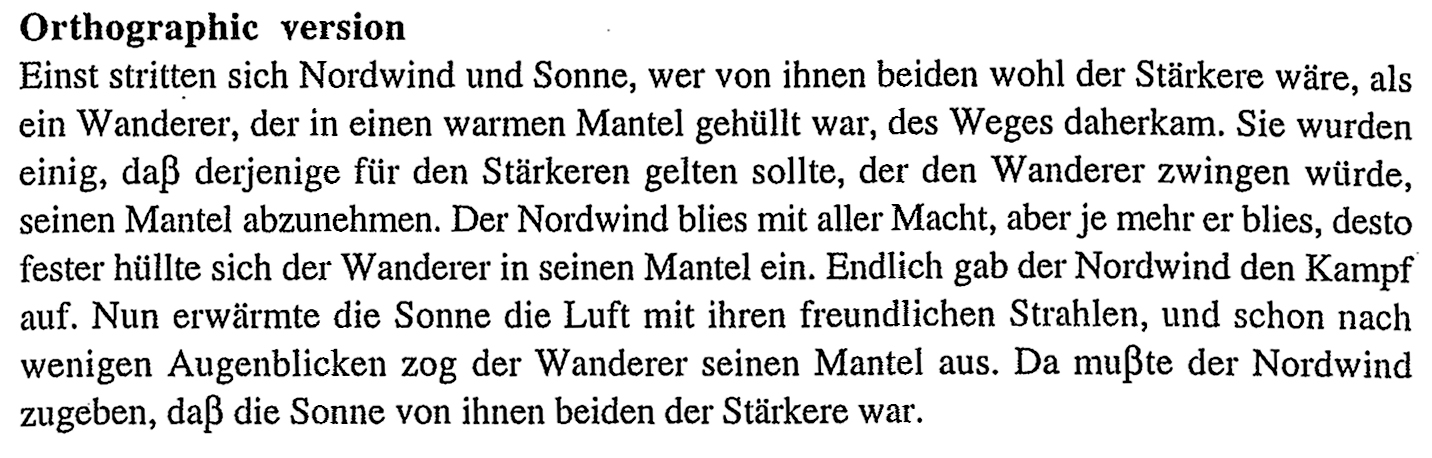
\includegraphics[scale=0.22]{material/04einststrittenorthopompino}
		\caption{\citep{Pompino95a}, \citep{Kohler99a}}
		%\label{Zeichen1}
	\end{figure}	
		
\end{frame}


%%%%%%%%%%%%%%%%%%%%%%%%%%%%%%%%%%%%%%%%%%%%%%%%%%%%%%%
\begin{frame}
\frametitle{Lösung}

Einst stritten sich Nordwind und Sonne, wer von ihnen beiden wohl der Stärkere wäre, als ein
Wanderer, der in einen warmen Mantel gehüllt war, des Weges daherkam. Sie wurden einig, dass
derjenige für den Stärkeren gelten sollte, der den Wanderer zwingen würde, seinen Mantel
abzunehmen. Der Nordwind blies mit aller Macht, aber je mehr er blies, desto fester hüllte sich der
Wanderer in seinen Mantel ein. Endlich gab der Nordwind den Kampf auf. Nun erwärmte die Sonne die
Luft mit ihrem freundlichen Strahlen, und schon nach wenigen Augenblicken zog der Wanderer seinen
Mantel aus. Da musste der Nordwind zugeben, dass die Sonne von ihnen beiden der Stärkere war.

\end{frame}

%%%%%%%%%%%%%%%%%%%%%%%%%%%%%%%%%%%%%%%%%%%%%%%%%%%%%%

\begin{frame}{\textipa{[ S l U s ]}}

	\begin{itemize}
		\item \textbf{VIDEO:} \href{run:material/04vocalcordssinging.wmv}{Vocal Cords}
	\end{itemize}
	
\end{frame}


%%%%%%%%%%%%%%%%%%%%%%%%%%%%%%%%%%%%%%%%%%%%%%%%%%%%%%%%%%%%%%%%
%%%%%%%%%%%%%%%%%%%%%%%%%%%%%%%%%%%%%%%%%%%%%%%%%%%%%%%%%%%%%%%%
%
\section{Elektronische Quellen}
%\frame{
%\begin{multicols}{2}
%\frametitle{~}
%	\tableofcontents[currentsection]
%\end{multicols}
%}
%%%%%%%%%%%%%%%%%%%%%%%%%%%%%%%%%%%%%%%%%%%%%%%%%%%%%%%%%%%%%%%%

\begin{frame}{Elektronische Quellen}
	\small
	
	\begin{itemize}
		\item VIDEO -- \gqq{Spoken Pirahã with subtitles} (Zugriff: 24.10.2013): \url{http://www.youtube.com/watch?v=SHv3-U9VPAs}
		\item LINK -- \gqq{Webseite der IPA} (Zugriff: 24.10.2013): \url{http://internationalphoneticassociation.org}
		\item LINK -- \gqq{Peter Ladefoged -- A Course in Phonetics} (Alle Laute zum Testen) (Zugriff: 24.10.2013):\\ \url{http://phonetics.ucla.edu/course/chapter1/chapter1.html}
		\item VIDEO -- \gqq{!Nama Clicks} (Zugriff: 24.10.2013): \url{http://www.youtube.com/watch?v=Ophrf64fxgA&list=PL6rcWnFnBuT7BEAex2IvI6l_bjLLycxaU}
		\item VIDEO -- \gqq{Anatomical Tutorial During Trans-Nasal Endoscopy} (Zugriff: 24.10.2012): \url{http://www.youtube.com/watch?v=wjRsa77u6OU}
		\item LINK -- \gqq{Interactive Sagittal Section} (Zugriff: 27.04.2016): \url{http://smu-facweb.smu.ca/~s0949176/sammy/}
		\item VIDEO -- \gqq{Vocal Cords up close while singing} (Zugriff: 24.10.2012): \url{http://www.youtube.com/watch?v=-XGds2GAvGQ}
	\end{itemize}
	
\end{frame}








%%%%%%%%%%%%%%%%%%%%%%%%%%%%%%%%%%%%%%%%%%%%%%%%%%%%
%%%             Metadata                         %%%
%%%%%%%%%%%%%%%%%%%%%%%%%%%%%%%%%%%%%%%%%%%%%%%%%%%%      

\title{Grundkurs Linguistik}

\subtitle{Phonologie\\Sprachgebildelautlehre}

\author[aMyP]{
	{\small Antonio Machicao y Priemer}
%	\\
%	{\footnotesize \url{http://www.linguistik.hu-berlin.de/staff/amyp}\\
%	\href{mailto:mapriema@hu-berlin.de}{mapriema@hu-berlin.de}}
}

\institute{Institut für deutsche Sprache und Linguistik}

%%%%%%%%%%%%%%%%%%%%%%%%%      
\date{ }
%\publishers{\textbf{6. linguistischer Methodenworkshop \\ Humboldt-Universität zu Berlin}}

%\hyphenation{nobreak}


%%%%%%%%%%%%%%%%%%%%%%%%%%%%%%%%%%%%%%%%%%%%%%%%%%%%
%%%             Preamble's End                   %%%
%%%%%%%%%%%%%%%%%%%%%%%%%%%%%%%%%%%%%%%%%%%%%%%%%%%%      


%%%%%%%%%%%%%%%%%%%%%%%%%      
\huberlintitlepage
\iftoggle{toc}{
\frame{
\begin{multicols}{2}
	\frametitle{Inhaltsverzeichnis}\tableofcontents
	%[pausesections]
\end{multicols}
}
}

%%%%%%%%%%%%%%%%%%%%%%%%%%%%%%%%%%%%%%%%%%%%%%%%%%%%%%%
%%%%%%%%%%%%%%%%%%%%%%%%%%%%%%%%%%%%%%%%%%%%%%%%%%%%%%%

\nocite{Repp&Co12a} 
\nocite{Hall00a} 
\nocite{Luedeling2009a} 
\nocite{Ramers08a}

%%%%%%%%%%%%%%%%%%%%%%%%%%%%%%%%%%%%%%%%%%%%%%%%%%%%%%%
%
\section{Einführung}
%
%\frame{
%\begin{multicols}{2}
%\frametitle{~}
%	\tableofcontents[currentsection]
%\end{multicols}
%}
%%%%%%%%%%%%%%%%%%%%%%%%%%%%%%%%%%%%%%%%%%%%%%%%%%%%%%%

\begin{frame}{Einführung}

\begin{itemize}
	\item Trennung von Phonetik und Phonologie: Ende der 1920er Jahre
	\item[]
	\item Strukturalistische Lehre der Prager Schule (vgl. \cite{Trubetzkoy89a})
	\item[]
	\item Unterscheidung auf allen Ebenen zwischen
	
	\begin{itemize}
		\item[]
		\item Sprachgebilde (zugrunde liegendes System \ras \textit{langue} -- später \textit{Kompetenz})
		\item[]
		\item[] und
		\item[]
		\item Sprechakt (tatsächliche Realisierung in einer Kommunikationssituation \textit{parole} -- später \textit{Performanz})
	\end{itemize}
	
\end{itemize}

\end{frame}



%%%%%%%%%%%%%%%%%%%%%%%%%%%%%%%%%%%%%%%%%%%%%%%%%%%%%%%

\begin{frame}
\frametitle{Einführung}

\begin{itemize}
	\item Phonetik: Untersuchung der materiellen Seite des Sprechens (Phone)
	\item[]
	\item Phonologie: Systematik der Laute \ras Materielle (messbare) Daten der Phonetik werden in abstrakterer Art und Weise \textbf{systematisiert}
	
	\begin{itemize}
		\item \textbf{Phoneminventar}: Bedeutungsunterscheidende Laute einer Sprache 

	\eal		
		\ex Im Dt. bedeutungsunterscheidend \textipa{[v]} und \textipa{[f]}: \textipa{[v\t{aI}n]} vs. \textipa{[f\t{aI}n]}
		\ex Deutsch: 16 Vokale \& 20 Konsonanten
		\ex Rotokas (Papua): 5 Vokale \& 6 Konsonanten
		\ex Mittelwert: 23 Konsonanten \& 8 Vokale
	\zl
	
		\item \textbf{Allophonie}: Vorkommen vs. Nicht-Vorkommen (bzw. Variation) von Lauten in bestimmten Kontexten

		\ea Wann kommt der \gqq{Ich-Laut} und wann der \gqq{Ach-Laut} vor?
		\z

	\end{itemize}
	
\end{itemize}
		
\end{frame}



%%%%%%%%%%%%%%%%%%%%%%%%%%%%%%%%%%%%%%%%%%%%%%%%%%%%%%%

\begin{frame}
\frametitle{Einführung}

\begin{itemize}
	\item \textbf{Phonologische Distribution}: An welchen Stellen kann ein Laut oder eine Lautfolge auftreten

	\ea \textipa{[St\textscr]} am Wortanfang aber nicht am Wortende \textipa{[St{\textscr}\t{aU}x]} \vs *\textipa{[\ldots aSt\textscr]}
	\z

	\item Phoneminventar, phonologische Distribution und Allophonie werden in der \textbf{strukturalistischen Phonologie} untersucht
	\item[]
	\item \textbf{Strukturalistische} Phonologie \ras Beschreibung von sprachlichen Daten 

\end{itemize}

\end{frame}


%%%%%%%%%%%%%%%%%%%%%%%%%%%%%%%%%%%%%%%%%%%%%%%%%%%%%%%

\begin{frame}
\frametitle{Einführung}

\begin{itemize}
	\item \textbf{Phonologische Prozesse}: Welche Lautfolgen, die an der Oberfläche unterschiedlich klingen, werden durch die Sprachnutzer trotzdem als Varianten eines zugrunde liegenden Musters erkannt?

\ea \textipa{[ga{\textscr}t@n]} \vs 
\textipa{[ga:d\textsyllabic{n}]}
\z

	\item \textbf{Generative} Phonologie $\rightarrow$ Zugrundeliegende Form +  Regeln ($\rightarrow$ Schlüsse über die allgemeine Sprachfähigkeit!) 
	\item[]
	\item Aufgaben des phonologischen Moduls:
	
	\begin{itemize}
		\item Bildung (und Verständnis) wohlgeformter Lautketten
		\item Inventar von Minimaleinheiten (Distinktive Merkmale -- hier Phoneme!)
		\item Regelinventar
	\end{itemize}
	 
\end{itemize}

\end{frame}



%%%%%%%%%%%%%%%%%%%%%%%%%%%%%%%%%%%%%%%%%%%%%%%%%%%%%%%

\begin{frame}
\frametitle{Einführung}

\begin{itemize}
	\item Weitere Untersuchungsgebiete der Phonologie:
	
	\begin{itemize}
		\item[]
		\item Eigenschaften von (lautlichen) Einheiten, die größer sind als ein Laut (\zB \textbf{Silbenphonologie})
		\item[]
		\item Wortakzent (\textbf{metrische Phonologie})
		\item[]
		\item Satzakzent, Phrasierung, Pausen, Sprechmelodie (\textbf{prosodische Phonologie}, Intonation)
	\end{itemize}
	
	\item[]
	\item Betrachtung der Laute \ras \textbf{lineare Phonologie}
	\item[]
	\item Analyse von einer Silbe \ras \textbf{nicht lineare (hierarchische) Phonologie}
\end{itemize}

\end{frame}



%%%%%%%%%%%%%%%%%%%%%%%%%%%%%%%%%%%%%%%%%%%%%%%%%%%%%%%
%%%%%%%%%%%%%%%%%%%%%%%%%%%%%%%%%%%%%%%%%%%%%%%%%%%%%%%
%
\section{Phonem, Phon, Allophon}
\iftoggle{toc}{
\frame{
\begin{multicols}{2}
\frametitle{~}
	\tableofcontents[currentsection]
\end{multicols}
}
}
%%%%%%%%%%%%%%%%%%%%%%%%%%%%%%%%%%%%%%%%%%%%%%%%%%%%%%%

\begin{frame}{Phonem, Phon, Allophon}

\begin{itemize}
	\item \textbf{Phon} (Notation \textipa{[ ]}):
	
	\begin{itemize}
		\item[]
		\item Minimaleinheit der Phonetik
		\item Physikalisch messbare lautliche Einheit einer Sprache
	\end{itemize}
	
	\item[]
	\item \textbf{Phonem} (Notation \textipa{/ /}):
	
	\begin{itemize}
		\item[]
		\item Minimaleinheit der Phonologie
		\item Abstraktes Konstrukt, das für eine \textbf{Menge} von möglichen Phonen (Allophonen) steht
		\item Resultat von \textbf{Systematisierung}
		\item Ermittelbar durch \textbf{Minimalpaarbildung} (strukturalistisches Kriterium)
		
	\begin{block}{Minimalpaar}
Wortpaar, das sich nur in einem Laut (eher Phonem) an der gleichen Stelle unterscheidet.
	\end{block}
	
	\end{itemize}
	
\end{itemize}

\end{frame}



%%%%%%%%%%%%%%%%%%%%%%%%%%%%%%%%%%%%%%%%%%%%%%%%%%%%%%%

\begin{frame}
\frametitle{Phonem, Phon, Allophon}

\begin{itemize}
	\item \textbf{Phonem} (Notation \textipa{/ /}):
	
	\begin{itemize}
		\item Ermittelbar durch \textbf{Minimalpaarbildung} (strukturalistisches Kriterium)
		
		\begin{block}{Minimalpaar}
Wortpaar, das sich nur in einem Laut (eher Phonem) an der gleichen Stelle unterscheidet
		\end{block}
	
	\eal
		\ex \label{schaf} \textipa{[Sa:l]}  \ab{Schal} vs. \textipa{[Sa:f]} \ab{Schaf}
		\ex\label{schall} \textipa{[Sa:l]} \ab{Schal} vs. \textipa{[Sal]} \ab{Schall}
		\ex \label{saal} \textipa{[Sa:l]} \ab{Schal} vs. \textipa{[za:l]} \ab{Saal}
	\zl
	
		\item \textbf{Phonologische Opposition}: Austausch der Laute wirkt sich bedeutungsunterscheidend (oder kategorieunterscheidend) aus.
	
	\eal
		\ex \textipa{/l/} vs. \textipa{/f/} in (\ref{schaf})
		\ex \textipa{/a:/} vs. \textipa{/a/} in (\ref{schall})
		\ex \textipa{/S/} vs. \textipa{/z/} in (\ref{saal})
	\zl			
	
	\end{itemize}
	
\end{itemize}

\end{frame}



%%%%%%%%%%%%%%%%%%%%%%%%%%%%%%%%%%%%%%%%%%%%%%%%%%%%%%%

\begin{frame}
\frametitle{Phonem, Phon, Allophon}

\begin{block}{Phonem (strukturalistisch)}
Kleinste bedeutungsunterscheidende Einheit eines Sprachsystems
\end{block}

\begin{itemize}
	\item Ein Phonem trägt keine Bedeutung. Es unterscheidet Bedeutungen!
	\item[]
	\item Phoneme sind immer Phoneme \textbf{einer Sprache / eines Systems}

	\eal
		\ex Deutsch: \textipa{[papa]} = \textipa{[p\super{h}ap\super{h}a]}
		\ex Hindi: \textipa{[pal]} ($\lsem$sich kümmern um$\rsem$) $\neq$ \textipa{[p\super{h}al]} ($\lsem$Messerblatt$\rsem$)
	\zl

\end{itemize}

\end{frame}



%%%%%%%%%%%%%%%%%%%%%%%%%%%%%%%%%%%%%%%%%%%%%%%%%%%%%%%

\begin{frame}
\frametitle{Phonem, Phon, Allophon}

\begin{itemize}
	\item \textbf{Allophone}:
	
	\begin{itemize}
		\item Phonetische Realisierungsvarianten \textbf{eines} Phonems
		
		\ea \textipa{[Sp r a:xe]} = \textipa{[Sp \textscr a:xe]} = \textipa{[Sp K a:xe]} \ras kein Bedeutungsunterschied
		\z

		\item \textbf{Komplementäre} Allophonie

	\eal
		\ex \textipa{[x]} \vs \textipa{[\c{c}]}
		\ex \textipa{[bax]} \vs \textipa{[mI\c{c}]}	
		\ex *\textipa{[mIx]} \vs *\textipa{[ba\c{c}]}
	\zl
	
		\item \textbf{Freie} Allophonie

		\ea \textipa{[p\super{h}as]} \vs \textipa{[pas]}
		\z
		
		\item \textbf{Regionale und soziale} Variation (Unterart der freien Allophonie)

		\ea \textipa{[PIS]} \vs \textipa{[PI\c{c}]}
		\z
		
	\end{itemize}
	
\end{itemize}

\end{frame}



%%%%%%%%%%%%%%%%%%%%%%%%%%%%%%%%%%%%%%%%%%%%%%%%%%%%%%%
%%%%%%%%%%%%%%%%%%%%%%%%%%%%%%%%%%%%%%%%%%%%%%%%%%%%%%%
%
\section{Phonetisch-phonologische Ebenen}
%
\iftoggle{toc}{
\frame{
\begin{multicols}{2}
\frametitle{~}
	\tableofcontents[currentsection]
\end{multicols}
}
}
%%%%%%%%%%%%%%%%%%%%%%%%%%%%%%%%%%%%%%%%%%%%%%%%%%%%%%%

\begin{frame}{Phonetisch-phonologische Ebenen}

	\begin{itemize}
		\item Unterscheidung von mindestens zwei Ebenen
		\item[$\rightarrow$] \textipa{[\textscr a: t]} und \textipa{[\textscr E: d 5]} (für \ab{Rad} und \abu{Räder})\\
		aber\\
		\textipa{[\textscr a: t]} und \textipa{[\textscr E: t @]} (für \ab{Rat} und \abu{Räte})
		\item[]
		\item[$\rightarrow$] Warum verstehen wir dasselbe, wenn wir\\
		\textipa{[h a: k @ n]} oder \textipa{[h a: k N]}\\
		hören?
		\item[]
		\item \textbf{Tiefenstruktur} (Deep Structure) vs. \textbf{Oberflächenstruktur} (Surface Structure)
	\end{itemize}
	
\end{frame}



%%%%%%%%%%%%%%%%%%%%%%%%%%%%%%%%%%%%%%%%%%%%%%%%%%%%%%%
%%%%%%%%%%%%%%%%%%%%%%%%%%%%%%%%%%%%%%%%%%%%%%%%%%%%%%%
%
\subsection{Tiefenstruktur (TS)}
%
%\frame{
%\begin{multicols}{2}
%\frametitle{~}
%	\tableofcontents[currentsection]
%\end{multicols}
%}
%%%%%%%%%%%%%%%%%%%%%%%%%%%%%%%%%%%%%%%%%%%%%%%%%%%%%%%

\begin{frame}{Tiefenstruktur (TS)}
	
\begin{itemize}
	\item \textbf{Zugrundeliegende abstrakte Repräsentation} $\rightarrow$ Phoneme \textipa{/ /}
	\item[]
	\item \textbf{Idiosynkratische} Form $\approx$ Nicht deriviert/abgeleitet
	\item[$\rightarrow$] Die TS-Form kann nicht durch Regeln abgeleitet werden, sie ist im Lexikon gespeichert.
	\item[]
	\item TS besteht aus Phonemen
	
	\eal
		\ex \textipa{/\textscr a: t/}: TS-Form von \ab{Rat}
		\ex \textipa{/\textscr a: d/}: TS-Form von \ab{Rad}
		\ex \textipa{/h a: k @ n/}: TS-Form von \ab{Haken}
	\zl
	
\end{itemize}
		
\end{frame}



%%%%%%%%%%%%%%%%%%%%%%%%%%%%%%%%%%%%%%%%%%%%%%%%%%%%%%%

\begin{frame}
\frametitle{Tiefenstruktur (TS)}

\begin{itemize}
	\item \textipa{[t]} in \textipa{[\textscr a: t]} (von \textipa{/\textscr a: d/}) ist ableitbar
	\item \textipa{/d/} in \textipa{/\textscr a: d/} ist idiosynkratisch
	\item[]
	\item \textipa{/t/} in \textipa{/\textscr a: t/} ist idiosynkratisch
	\item[]
	\item Wenn das Deutsche ein neues Wort wie \ab{Code} \textipa{[k @ U d]} entlehnen würde, würde dieses Wort früher oder später \gqq{eingedeutscht} werden.
	
	\ea \textipa{[k O U t]} oder \textipa{[k o: t]} aber \gqq{des \textipa{[k O U d @ s]}} oder \gqq{des \textipa{[k o: t s]}} 
	\z
	
\end{itemize}

\end{frame}



%%%%%%%%%%%%%%%%%%%%%%%%%%%%%%%%%%%%%%%%%%%%%%%%%%%%%%%
%%%%%%%%%%%%%%%%%%%%%%%%%%%%%%%%%%%%%%%%%%%%%%%%%%%%%%%
%
\subsection{Oberflächenstruktur (OS)}
%
%\frame{
%\begin{multicols}{2}
%\frametitle{~}
%	\tableofcontents[currentsection]
%\end{multicols}
%}
%%%%%%%%%%%%%%%%%%%%%%%%%%%%%%%%%%%%%%%%%%%%%%%%%%%%%%%

\begin{frame}{Oberflächenstruktur (OS)}

\begin{itemize}
	\item Von der abstrakten phonembasierten TS wird die sog. Oberflächenstruktur mithilfe von vorhersagbaren (phonetisch-)phonologischen Regeln deriviert.
	\item[]
	\item OS entspricht der \textbf{tatsächlichen Realisierung} $\rightarrow$ Phone \textipa{[ ]}
	\item[]
	\item Demnach gibt es viele mögliche OS-Formen, darunter auch die sog.\\ 
\textbf{kanonische Aussprache} ($\approx$ Standardaussprache) $\rightarrow$ \textipa{[P e: b @ n]},\\
und die vielen möglichen\\
\textbf{umgangssprachlichen Formen} $\rightarrow$ \textipa{[P e: b n]}, \textipa{[P e: b m]}, \textipa{[P e: m]}
	\item[]
	\item Häufig wird zwischen phonologischen und phonetischen Prozessen unterschieden.
\end{itemize}

\end{frame}



%%%%%%%%%%%%%%%%%%%%%%%%%%%%%%%%%%%%%%%%%%%%%%%%%%%%%%%

\begin{frame}
\frametitle{{Oberflächenstruktur (OS)}}

\begin{itemize}
	\item Häufig wird zwischen phonologischen und phonetischen Prozessen unterschieden.
	\item[]
	\item \textbf{Phonetische Prozesse} $\rightarrow$ vom Sprachtempo und Stil abhängige Veränderungen
	\item[$\rightarrow$] Plosiveinsetzung: \textipa{/a m t/} $\rightarrow$ \textipa{[P a m p t]}
	\item[]
	\item \textbf{Phonologische Prozessen} $\rightarrow$ systematisch und obligatorisch auftretende Veränderungen
	\item[$\rightarrow$] \textit{Ich}-/\textit{Ach}-Laut-Wechsel \textipa{[b u: x]} (von \textipa{/b u: \c{c}/}) ist ableitbar
	\item[]
	\item Einen klaren Schnitt zwischen phonetischen und phonologischen Prozessen gibt es nicht!
	\item[$\rightarrow$] Sind g-Tilgung, Spirantisierung, Schwa-Tilgung, \dots phonetische oder phonologische Prozesse?
\end{itemize}

\end{frame}



%%%%%%%%%%%%%%%%%%%%%%%%%%%%%%%%%%%%%%%%%%%%%%%%%%%%%%%
%%%%%%%%%%%%%%%%%%%%%%%%%%%%%%%%%%%%%%%%%%%%%%%%%%%%%%%
%
\subsection{TS \& OS}
%
%%%%%%%%%%%%%%%%%%%%%%%%%%%%%%%%%%%%%%%%%%%%%%%%%%%%%%%
%\frame{
%\frametitle{~}
%	\tableofcontents[currentsection]
%}
%%%%%%%%%%%%%%%%%%%%%%%%%%%%%%%%%%%%%%%%%%%%%%%%%%%%%%%

\begin{frame}{TS \& OS}

\begin{itemize}
	\item TS \& OS sind \textbf{theoretische Abstraktionen} ($\approx$ keine Wahrheiten!), um die Regelhaftigkeiten auf der phonologischen Ebene erklären zu können.
	\item[]
	\item Kind erhält als \textbf{Input im Spracherwerb} OS-Formen wie: \textipa{[\textscr a: t]} und \textipa{[\textscr E: t @]}, \textipa{[\textscr a: t]} und \textipa{[\textscr E: d 5]}, \textipa{[b E t]} und \textipa{[b E t @ n]}, \textipa{[b a: t]} und \textipa{[b E: d 5]}, \textipa{[k I n t]} und \textipa{[k I n d 5]}
	\item[]
	\item Daraus erkennt das Kind,

	\begin{itemize}
		\item dass in einigen Wörtern \textipa{[d]} und \textipa{[t]} \textbf{systematisch} ausgetauscht werden (\zB \ab{Rad}, \ab{Bad}, \ab{Kind}),
		\item dass aber in anderen Wörtern \textipa{[t]} immer als \textipa{[t]} ausgesprochen wird  (\zB \ab{Rat}, \ab{Bett}).
	\end{itemize}
		
\end{itemize}

\end{frame}



%%%%%%%%%%%%%%%%%%%%%%%%%%%%%%%%%%%%%%%%%%%%%%%%%%%%%%%

\begin{frame}
	\frametitle{TS \& OS}
		
\begin{itemize}
	\item Daraus erkennt das Kind,
	
	\begin{itemize}
		\item dass in einigen Wörtern \textipa{[d]} und \textipa{[t]} \textbf{systematisch} ausgetauscht werden (z.~B. \ab{Rad}, \ab{Bad}, \ab{Kind}),
		\item dass aber in anderen Wörtern \textipa{[t]} immer als \textipa{[t]} ausgesprochen wird  (z.~B. \ab{Rat}, \ab{Bett}).
		\item[]
		\item Daraus leitet das Kind Folgendes ab:
		\item[$\rightarrow$] \textipa{/d/} $\rightarrow$ \textipa{[t]} am Ende des Wortes (bzw. der Silbe)!
		\item[]
		\item[] Aber nicht:
		\item[]
		\item[$\rightarrow$] \textipa{/t/} $\rightarrow$ \textipa{[d]}\\ (Andernfalls müsste der Plural von \ab{Rat} \gqq{die \textipa{[\textscr E: d @]}} heißen.)
	\end{itemize}
	
	\item[]
	\item Diese Regelhaftigkeit erweitert das Kind auf weitere Lauteinheiten bei weiterem Input $\rightarrow$ \textipa{/b d g z v Z/}	(sog. stimmhafte Obstruenten)
\end{itemize}

\end{frame}
	


%%%%%%%%%%%%%%%%%%%%%%%%%%%%%%%%%%%%%%%%%%%%%%%%%%%%%%%

\begin{frame}
\frametitle{TS \& OS}

\begin{table}
\centering 
		
\begin{tabular}{p{0.17\linewidth}p{0.15\linewidth}p{0.17\linewidth}p{0.15\linewidth}p{0.17\linewidth}}
	\hline
	\textbf{TS}\par \tiny{Phonologische\par Repräsentation\ (Lexikon)} & & \textbf{OS}\par \tiny{Phonetische\par Repräsentation\par (Standard)} & & \textbf{OS}\par \tiny{Phonetische\par Repräsentation\par (Umgangssprache)} \\
	\hline
	\textipa{/\textscr a: d/} & $\begin{array}[c]{c}\rightarrow\end{array}$ & \textipa{[\textscr a: t]} & & \\
	\hline
	\textipa{/\textscr a: t/} & $\begin{array}[c]{c}\rightarrow\end{array}$ & \textipa{[\textscr a: t]} & & \\
	\hline
	\textipa{/e: b @ n/} & $\begin{array}[c]{c}\rightarrow\end{array}$ & \textipa{[P e: b @ n]} & $\begin{array}[c]{c}\rightarrow\end{array}$ & \textipa{[P e: b m]}\\
	\hline
	& \small{Phonologische\par Prozesse} &  & \small{Phonetische\par Prozesse} & \\
	\hline		
\end{tabular}

\caption{TS $\rightarrow$ OS} 
\end{table}

\begin{itemize}
	\item Die Abstraktion (s. Tabelle) impliziert eine gewisse zeitliche Abfolge, die es in der Realität nicht gibt. Es handelt sich um eine theoretische Abstraktion, die notwendig ist, um Phänomene zu erfassen!	
\end{itemize}
			
\end{frame}


%%%%%%%%%%%%%%%%%%%%%%%%%%%%%%%%%%%%%%%%%%%%%%%%%%%%%%%
%%%%%%%%%%%%%%%%%%%%%%%%%%%%%%%%%%%%%%%%%%%%%%%%%%%%%%%
%
\section{Phonetisch/phonologische Prozesse}
%
%%%%%%%%%%%%%%%%%%%%%%%%%%%%%%%%%%%%%%%%%%%%%%%%%%%%%%%
%\frame{
%\frametitle{~}
%	\tableofcontents[currentsection]
%}
%%%%%%%%%%%%%%%%%%%%%%%%%%%%%%%%%%%%%%%%%%%%%%%%%%%%%%%

\begin{frame}{Phonetisch/phonologische Prozesse}

\begin{itemize}
	\item Tilgung von Segmenten
	\item[]
	\item Hinzufügung von Segmenten
	\item[]
	\item Veränderung von Segmenten
	\item[]
	\item Allgemeine Notation: A \ras B / C \underline{\quad} D
	\item[] Ein Segment A im Input wird zu einem Segment B im Output in einem Kontext (\gqq{/}), in dem C \textit{vor} und D \textit{nach} A vorkommt. 
\end{itemize}

\end{frame}



%%%%%%%%%%%%%%%%%%%%%%%%%%%%%%%%%%%%%%%%%%%%%%%%%%%%%%%
%%%%%%%%%%%%%%%%%%%%%%%%%%%%%%%%%%%%%%%%%%%%%%%%%%%%%%%
%
\subsection{Tilgung von Segmenten}
%
%%%%%%%%%%%%%%%%%%%%%%%%%%%%%%%%%%%%%%%%%%%%%%%%%%%%%%%
%\frame{
%\frametitle{~}
%	\tableofcontents[currentsection]
%}
%%%%%%%%%%%%%%%%%%%%%%%%%%%%%%%%%%%%%%%%%%%%%%%%%%%%%%%

\begin{frame}{Tilgung von Segmenten}

\begin{itemize}
	\item \textbf{\textipa{/@/}-Tilgung}:
	
	\begin{itemize}
		\item Fakultativ
		\item Regel: \textipa{/@/} \ras $\emptyset$ / X \underline{\quad} $\{$[sonorant]; absoluter Auslaut$\}$
	
	\eal
		\ex \ab{gehen}: \textipa{/ge:.@n/} \ras \textipa{[ge:n]}
		\ex \ab{kaufe}: \textipa{/k\t{aU}.f@/} \ras \textipa{[k\t{aU}f]}
		\ex \ab{Kumpel}: \textipa{/kUm.p@l/} \ras \textipa{[kUm.p\textsyllabic{l}]}
	\zl
	
	\end{itemize}

	\item \textbf{\textipa{/g/}-Tilgung}:
	
	\begin{itemize}
		\item Obligatorisch
		\item Regel: \textipa{/g/} \ras $\emptyset$ / [nasal, velar] \underline{\quad} $]_\sigma$
		
		\ea \ab{Tilgung}: \textipa{[tIl.gUNg]} \ras \textipa{[tIl.gUN]}
		\z
		
	\end{itemize}
			
\end{itemize}

\end{frame}


%%%%%%%%%%%%%%%%%%%%%%%%%%%%%%%%%%%%%%%%%%%%%%%%%%%%%%%

\begin{frame}
\frametitle{Tilgung von Segmenten}

\begin{itemize}
	\item \textbf{Geminatenreduktion}:

	\begin{itemize}
		\item Fakultativ
		\item Regel: XX \ras X / A \underline{\quad} B

	\eal
		\ex \abu{Enttäuschung}: \textipa{/Ent.t\t{OI}.SUng/} \ras \textipa{[PEn\.t\t{OI}.SUN]}
		\ex \ab{Schifffahrt}: \textipa{/SIf.fa:{\textscr}t/} \ras \textipa{[SI\.fa:{\textscr}t]}
		\ex ABER \ab{Zoooper}: \textipa{/\t{ts}o:.o.p@{\textscr}/} \ras \textipa{[\t{ts}o:.Po.p5]}
	\zl
	
	\end{itemize}
	
\end{itemize}

\end{frame}



%%%%%%%%%%%%%%%%%%%%%%%%%%%%%%%%%%%%%%%%%%%%%%%%%%%%%%%
%%%%%%%%%%%%%%%%%%%%%%%%%%%%%%%%%%%%%%%%%%%%%%%%%%%%%%%
%
\subsection{Hinzufügung von Segmenten}
%
%\frame{
%\begin{multicols}{2}
%\frametitle{~}
%	\tableofcontents[currentsection]
%\end{multicols}
%}
%%%%%%%%%%%%%%%%%%%%%%%%%%%%%%%%%%%%%%%%%%%%%%%%%%%%%%%

\begin{frame}{Hinzufügung von Segmenten}

\begin{itemize}
	\item Allgemeine Regel: $\emptyset$ \ras X / A \underline{\quad} B
	\item[]
	\item \textbf{Plosiveinsetzung}:
	
	\begin{itemize}
		\item Fakultativ
		
	\eal
		\ex \ab{Amt}: \textipa{/amt/} \ras \textipa{[Pampt]}
		\ex \ab{Gans}: \textipa{/gans/} \ras \textipa{[gants]}
	\zl
	
	\end{itemize}

	\item \textbf{Knacklauteinsetzung}:

	\begin{itemize}
		\item (Fast) Obligatorisch
		\item Plosiveinsetzung
		\item Regel: $\emptyset$ \ras \textipa{[P]} / 
		$\{$\#; \textprimstress$_\sigma[\}$ 
\underline{\quad} V

	\eal
		\ex \ab{Beamte}: \textipa{/b@.\textprimstress am.t@/} \ras \textipa{[b@.\textprimstress Pam.t@]}
		\ex \ab{Apfel}: \textipa{/a\t{pf}@l/} \ras \textipa{[Pa\t{pf}@l]}
		\ex ABER \ab{gehen}: \textipa{/\textprimstress ge:.@n/} $\nrightarrow$ \textipa{[\textprimstress ge:.P@n]} sondern: \textipa{[\textprimstress ge:.@n]}
	\zl
	
	\end{itemize}
			
\end{itemize}

\end{frame}



%%%%%%%%%%%%%%%%%%%%%%%%%%%%%%%%%%%%%%%%%%%%%%%%%%%%%%%
%%%%%%%%%%%%%%%%%%%%%%%%%%%%%%%%%%%%%%%%%%%%%%%%%%%%%%%
%
\subsection{Veränderung von Segmenten (durch Assimilation)}
%
%\frame{
%\begin{multicols}{2}
%\frametitle{~}
%	\tableofcontents[currentsection]
%\end{multicols}
%}
%%%%%%%%%%%%%%%%%%%%%%%%%%%%%%%%%%%%%%%%%%%%%%%%%%%%%%%

\begin{frame}{Veränderung von Segmenten (durch Assimilation)}

\begin{itemize}
	\item \textbf{Regressive velare Nasalassimilation}

	\begin{itemize}
		\item Obligatorisch (innerhalb des phonologischen Wortes)
		\item Regel: \textipa{/n/} \ras \textipa{[N]} /  \underline{\quad} [velar, plosiv]

	\eal		
		\ex \abu{Führung}: \textipa{/fy:.{\textscr}Ung/} \ras \textipa{[fy:.{\textscr}UNg]} (nach g-Tilgung \ras \textipa{[fy:.{\textscr}UN]})
		\ex \ab{Bank}: \textipa{/bank/} \ras \textipa{[baNk]}
		\ex ABER \ab{ungern}: \textipa{/Un.gE{\textscr}n/} \ras \textipa{[PUn.gE{\textscr}n]} oder fakulativ \textipa{[PUN.gE{\textscr}n]}
	\zl
	
	\end{itemize}
	
	\item[]
	\item \textbf{(Allgemeine) regressive Nasalassimilation}:

	\begin{itemize}
		\item Fakultativ
		\item Regel: [nasal, Art.Ort: Y] \ras [nasal, Art.Ort: X] /  \underline{\quad} [obstruent, Art.Ort: X]

		\ea \abu{fünf}: \textipa{/fYnf/} \ras \textipa{[fYmf]}
		\z
		
	\end{itemize}		

\end{itemize}

\end{frame}



%%%%%%%%%%%%%%%%%%%%%%%%%%%%%%%%%%%%%%%%%%%%%%%%%%%%%%%

\begin{frame}
{Veränderung von Segmenten (durch Assimilation)}

\begin{itemize}
	\item \textbf{Progressive Nasalassimilation}:

	\begin{itemize}
		\item Fakultativ
		\item Regel: [nasal, Art.Ort: Y] $\rightarrow$ [nasal, Art.Ort: X] /  [obstruent, Art.Ort: X] \underline{\quad} 

	\eal
		\ex \ab{Haken}: \textipa{/ha:k@n/} \ras 
		\textipa{[ha:k\textsyllabic{n}]} \ras \textipa{[ha:k\textsyllabic{N}]}
		\ex \ab{Schuppen}: \textipa{/SUp@n/} \ras 
		\textipa{[SU\.p\textsyllabic{n}]} \ras \textipa{[SU\.p\textsyllabic{m}]}
	\zl
	
	\end{itemize}

	\item[]
	\item \textbf{\textipa{[\c{c}]/[x]}-Alternation (Dorsale Assimilation)}

	\begin{itemize}
		\item Obligatorisch
		\item Regel: \textipa{/\c{c}/} $\rightarrow$ \textipa{[x]} / Hinterer Vokal \underline{\quad}

	\eal
		\ex \ab{mich}: \textipa{/mI\c{c}/} $\rightarrow$ \textipa{[mI\c{c}]}
		\ex \ab{Buch}: \textipa{/bU\c{c}/} $\rightarrow$ \textipa{[bUx]}
		\ex \ab{Elch}: \textipa{/El\c{c}/} $\rightarrow$ \textipa{[PEl\c{c}]}
	\zl
	
	\end{itemize}		

\end{itemize}

\end{frame}



%%%%%%%%%%%%%%%%%%%%%%%%%%%%%%%%%%%%%%%%%%%%%%%%%%%%%%%

\begin{frame}
\frametitle{Veränderung von Segmenten (durch Assimilation)}

\begin{itemize}
	\item \textbf{\textipa{/g/}-Spirantisierung}

	\begin{itemize}
		\item Fakultativ (dialektal)
		\item Regel: \textipa{/g/} \ras \textipa{/\c{c}/} / V\underline{\quad} $]_\sigma$

\eal	
	\ex \ab{sagst}: \textipa{/za:gst/} $\rightarrow$ \textipa{[za:xst]}
	\ex \ab{freudig}: \textipa{/f{\textscr}\t{OI}.dIg/} $\rightarrow$ \textipa{[f{\textscr}\t{OI}.dI\c{c}]}
\zl

	\end{itemize}

	\item[]
	\item \textbf{\textipa{/{\textscr}/}-Vokalisierung}
	
	\begin{itemize}
		\item Fakultativ -- Obligatorisch
		\item Regel: \textipa{/{\textscr}/} \ras \textipa{[5]} / V\underline{\quad} $]_\sigma$

	\eal
		\ex \ab{Ohr}: \textipa{/o:{\textscr}/} $\rightarrow$ \textipa{[Po:5]}
		\ex \ab{fern}: \textipa{/fE{\textscr}n/} $\rightarrow$ \textipa{[fE5n]}
		\ex \ab{Lehrer}: \textipa{/le:.{\textscr}@{\textscr}/} $\rightarrow$ \textipa{[le:.{\textscr}@5]} (nach Schwa-Tilgung $\rightarrow$ \textipa{[le:.{\textscr}5]}
	\zl
	
	\end{itemize}

\end{itemize}

\end{frame}



%%%%%%%%%%%%%%%%%%%%%%%%%%%%%%%%%%%%%%%%%%%%%%%%%%%%%%%

\begin{frame}
{Veränderung von Segmenten (durch Assimilation)}

\begin{itemize}
	\item \textbf{Auslautverhärtung}

	\begin{itemize}
		\item Obligatorisch
		\item Regel: /obstruent, stimmhaft/ \ras [obstruent, stimmlos] / \underline{\quad} $]_\sigma$

	\eal
		\ex \ab{Bad}: \textipa{/ba:d/} \ras \textipa{[ba:t]}
		\ex ABER \abu{Bäder}: \textipa{/bE:.d@{\textscr}/} \ras \textipa{[bE:.d5]}
		\ex \ab{oliv}: \textipa{/oli:v/} \ras \textipa{[Po.li:f]}
		\ex ABER \ab{Olive}: \textipa{/oli:v@/} \ras \textipa{[Po.li:.v@]}
		\ex \ab{Endspurt}: \textipa{/End.SpU{\textscr}t/} \ras \textipa{[PEnt.SpU{\textscr}t]}
		\ex ABER \ab{Ende}: \textipa{/En.d@/} \ras \textipa{[PEn.d@]}
	\zl
	
	\end{itemize}

\end{itemize}

\end{frame}



%%%%%%%%%%%%%%%%%%%%%%%%%%%%%%%%%%%%%%%%%%%%%%%%%%%%%%%
%%%%%%%%%%%%%%%%%%%%%%%%%%%%%%%%%%%%%%%%%%%%%%%%%%%%%%%
%
\subsection{Reihenfolge der Prozesse}
%
%\frame{
%\begin{multicols}{2}
%\frametitle{~}
%	\tableofcontents[currentsection]
%\end{multicols}
%}
%%%%%%%%%%%%%%%%%%%%%%%%%%%%%%%%%%%%%%%%%%%%%%%%%%%%%%%

\begin{frame}{Reihenfolge der Prozesse}

\begin{itemize}
	\item Reihenfolge der Prozesse spielt eine wichtige Rolle!

	\begin{block}{Feeding}
	Wenn ein Prozess die kontextuellen Bedingungen für einen weiteren Prozess \textbf{schafft}.	

	\end{block}

	\ea \ab{Haken}: \textipa{/ha:k@n/} \ras \textipa{[ha:k\textsyllabic{n}]} \ras \textipa{[ha:k\textsyllabic{N}]}
	\z

	\begin{block}{Bleeding}
	Wenn ein Prozess die kontextuellen Bedingungen für einen weiteren Prozess \textbf{zerstört}.
	\end{block}

	\ea \ab{Gesang}: \textipa{/g@.zang/} \ras \textipa{[g@.zaNg]} \ras \textipa{[g@.zaN]} $\nrightarrow$ \textipa{[g@.zaNk]}
	\z
	
\end{itemize}

\end{frame}




\exewidth{\exnrfont(235)}
%\exewidth{(35)} im übergeordneten File

% sollte zentral geladen werden. St. Mü. 04.11.2016 (in localcommands?)
%%%%%%%%%%%%%
%%% Forestset Syllables

\newbox\foreststrutbox
\setbox\foreststrutbox=\hbox to 0pt{\phantom{\forestOve{standard node}{content}}}
\def\foreststrut{\copy\foreststrutbox}
\forestset{
GP1/.style 2 args={
for n={1}{baseline},
s sep=0pt, l sep=0pt,
for descendants={
l sep=0pt, l={#1},
anchor=base,calign=first,child anchor=north,
inner xsep=1pt,inner ysep=2pt,outer sep=0pt,s sep=0pt,
},
delay={
if content={}{phantom}{for children={no edge}},
for tree={
if content={O}{tier=OR}{},
if content={R}{tier=OR}{},
if content={N}{tier=N}{},
if content={x}{
tier=x,content={$\times$},outer xsep={#2},
for tree={calign=center},
for descendants={content format={\foreststrut\forestoption{content}}},
before drawing tree={outer xsep=0pt,delay={typeset node}},
s sep=4pt
}{},
},
},
before drawing tree={where content={}{parent anchor=center,child anchor=center}{}},
},
GP1/.default={5ex}{8.0pt},
associate/.style={%
tikz+={\draw(!)--(!#1);}},
spread/.style={
before drawing tree={tikz+={\draw[dotted](!)--(!#1);}}},
govern/.style={
before drawing tree={tikz+={\draw[->](!)--(!#1);}}},
p-govern/.style={
before drawing tree={tikz+={\draw[->](.north) to[out=150,in=30] (!#1.north);}}},
no p-govern/.style={
before drawing tree={tikz+={\draw[->,loosely dashed](.north) to[out=150,in=30] (!#1.north);}}},
encircle/.style={before drawing tree={circle,draw,inner sep=0pt}},
fen/.style={pin={[font=\footnotesize,inner sep=1pt,pin edge=<-]10:\textsc{Fen}}},
el/.style={content=\textsc{\textbf{##1}}},
head/.style={content=\textsc{\textbf{\underline{##1}}}},
llap/.style={
tikz+={%
\edef\forest@temp{\noexpand\node[\option{node options},
anchor=base east,at=(.base east)]}%
\forest@temp{#1\phantom{\option{environment}}};
}
},
rlap/.style={
tikz+={%
\edef\forest@temp{\noexpand\node[\option{node options},
anchor=base west,at=(.base west)]}%
\forest@temp{\phantom{\option{environment}}#1};
}
},
}
%%%%%%%%%%%%%



%%%%%%%%%%%%%%%%%%%%%%%%%%%%%%%%%%%%%%%%%%%%%%%%%%%%
%%%             Metadata                         %%%
%%%%%%%%%%%%%%%%%%%%%%%%%%%%%%%%%%%%%%%%%%%%%%%%%%%%      


\title{Grundkurs Linguistik}

\subtitle{Phonologie II: Silbe}

\section{Phonologie II: Silbe}

\author[aMyP]{Antonio Machicao y Priemer%
	\\
	{\footnotesize %\url{http://www.linguistik.hu-berlin.de/staff/amyp}\\
	\href{mailto:mapriema@hu-berlin.de}{mapriema@hu-berlin.de}}
}

%\institute{Institut für deutsche Sprache und Linguistik}

%%%%%%%%%%%%%%%%%%%%%%%%%      
%\date{ }
%\publishers{\textbf{6. linguistischer Methodenworkshop \\ Humboldt-Universität zu Berlin}}

%\hyphenation{nobreak}


%%%%%%%%%%%%%%%%%%%%%%%%%%%%%%%%%%%%%%%%%%%%%%%%%%%%
%%%             Preamble's End                   %%%
%%%%%%%%%%%%%%%%%%%%%%%%%%%%%%%%%%%%%%%%%%%%%%%%%%%%      

\huberlintitlepage[22pt]

%\frame{\titlepage}

%% %%%%%%%%%%%%%%%%%%%%%%%%%      
%% \begin{frame}
%%   \HUtitle
%% \end{frame}

\iftoggle{toc}{
\frame{
\begin{multicols}{2}
	\frametitle{Inhaltsverzeichnis}\tableofcontents
	%[pausesections]
\end{multicols}
}
}

%%%%%%%%%%%%%%%%%%%%%%%%%%%%%%%%%%%
%%%%%%%%%%%%%%%%%%%%%%%%%%%%%%%%%%
%%\subsection{Kontakt}
%\frame{
%\begin{multicols}{2}
%\frametitle{~}
%	\tableofcontents[currentsection]
%\end{multicols}
%}
%%%%%%%%%%%%%%%%%%%%%%%%%%%%%%%%%%

%% \begin{frame}
%% \frametitle{Kontakt}


%% \scalebox{0.95}{

%% \begin{tabular}{ll}
%% \textbf{Dozent:} & Antonio Machicao y Priemer \\ 
%% 			     & \textipa{[ma.\t{tS}i."ka.o.\textprimstress Pi."p\textscr i:.m5]}\\
%% \textbf{E-Mail:} & \href{mailto:mapriema@hu-berlin.de}{mapriema@hu-berlin.de} \\ 
%% \textbf{Webseite:} & \url{http://www.linguistik.hu-berlin.de/staff/amyp} \\ 
%% \textbf{Büro:} & Dorotheenstraße 24, Raum: 3.305 \\ 
%% \textbf{Telefonnummer:} & +49(30)-2093-9702 \\
%% \textbf{Sprechstunde:} & Mittwochs 10--12 (Anmeldung per E-Mail erforderlich!) \\ 
%%  & \\
%% \textbf{Sekretariat:} & Anina Klein \\	
%% \textbf{E-Mail:} & \href{mailto:Anina.Klein@cms.hu-berlin.de}{Anina.Klein@cms.hu-berlin.de} \\
%% \textbf{Büro:} & Dorotheenstraße 24, Raum: 3.306 \\
%% \textbf{Telefonnummer:} & +49(30)-2093-9639 \\
%% \end{tabular} 

%% }
%% \end{frame}



%%%%%%%%%%%%%%%%%%%%%%%%%%%%%%%%%%
%%%%%%%%%%%%%%%%%%%%%%%%%%%%%%%%%%
\subsection{Einführung}
%\frame{
%\begin{multicols}{2}
%\frametitle{~}
%	\tableofcontents[currentsection]
%\end{multicols}
%}
%%%%%%%%%%%%%%%%%%%%%%%%%%%%%%%%%%%
%% LITERATUR
\nocite{Altmann&Co07a} \nocite{Hall00a} \nocite{Pompino95a} \nocite{Ramers08a} \nocite{Repp&Co12a} \nocite{WieseR96a} \nocite{WieseR11a}
%%%%%%%%%%%%%%%%%%%%%%%%%%%%%%%%%%%

\begin{frame}
\frametitle{Begleitlektüre}
\begin{itemize}
	\item AM S.~24--28
	\item \citet[Kapitel~8]{Hall00a}:  S.~205--230; 238--254)
\end{itemize}
\end{frame}

%%%%%%%%%%%%%%%%%%%%%%%%%%%%%%%%%%%



\begin{frame}
\frametitle{Einführung: Notation}


\begin{itemize}
	\item Graphematische Notation in spitzen Klammern: 
	
	  \ea
          \ab{nordwind}, \ab{Nordwind}
          \z
% zwei Varianten, eine phonographisches Prinzip, eine mit syntaktischer Info = Großschreibung
          
	\item[]	
	\item Phonetische Notation in eckigen Klammern:
	
	  \ea
          \textipa{[nO5t.vInt]}
	  \z
          
	\item[]
	\item Phonologische Notation in Schrägstrichen:
	
	  \ea
          \textipa{/nO\textscr d.vInd/}
	  \z
\end{itemize}

\end{frame}



%%%%%%%%%%%%%%%%%%%%%%%%%%%%%%%%%%%
\begin{frame}
\frametitle{Einführung: Silben}


Warum nimmt man Silben an?

\begin{itemize}
	\item Die Auslautverhärtung mit Bezug auf das Wort (vorläufig):
	
	  \ea
             {}[$-$son] $\rightarrow$ [$-$sth] /\_\_ \#
	     \z
	\item Transkribieren Sie: (\emph{sie}) \emph{siegte}

% Auslautverhärtung auch bei Silben
\pause	
\ea
\textipa{[zi:k . t@]} (\gqq{.} steht für Silbengrenze)
\z

\pause
	\eal 
	\ex \textipa{[St\textscr e:p.za:m]} \vs \textipa{[St\textscr e:.b5]}
	\ex \textipa{[bYnt.nIs]} \vs \textipa{[bUn.d@s]}
	\ex \textipa{[bi:k.za:m]} \vs \textipa{[bi:.g@n]}
	\ex \textipa{[le:s.b5]} \vs \textipa{[le:.z@n]}
        \zl
        
	\item Auslautverhärtung mit Bezug auf die \textbf{Silbe}:
	  \ea
             {}[$-$son] $\rightarrow$ [$-$sth] /\_\_ $]_{\sigma}$
	  \z	
\end{itemize}


\end{frame}



%%%%%%%%%%%%%%%%%%%%%%%%%%%%%%%%%%%

\begin{frame}
\frametitle{Silben}

Warum nimmt man Silben an?

Silbe als \textbf{Domäne} \ldots

\begin{itemize}	
	\item \ldots\ verschiedener \textbf{phonologischer Prozesse}\\
               (\zB Auslautverhärtung, Knacklauteinsetzung, Aspiration, \ldots )
	
	\item[] 
	
	\item \ldots\ von Regularitäten bzgl. der \textbf{Abfolge} von Lauten
	
	\item[]
	
	\item \ldots\ der \textbf{Wortbetonung}, d.\,h. wichtige so genannte prosodische Einheiten (Prosodie = Bezug auf Einheiten über dem Segment)
\end{itemize}

\end{frame}



%%%%%%%%%%%%%%%%%%%%%%%%%%%%%%%%%%%

\begin{frame}
\frametitle{Prosodische Konstituenten}

	\begin{multicols}{2}
	\begin{itemize}
		\item UP = Äußerungsphrase
		\item IP = Intonationsphrase
		\item $\phi$ = phonol. Phrase
\columnbreak
		\item $\omega$ = phonol. Wort
		\item F = phonol. Fuß
		\item \alertred{$\sigma$ = Silbe}
	\end{itemize}
	\end{multicols}

\begin{figure} %%rote Box einfügen
	\centering
	\scalebox{.65}{
	\begin{forest} MyP edges,
	[IP
	[$\Phi$
	[$\omega$[F[\alertred{$\sigma$}[Frau]]]]
	[$\omega$[F[\alertred{$\sigma$}[Müll, name=mueller]][\alertred{$\sigma$}, name=sigma[er]]]]]
	[$\Phi$
	[$\omega$[F[\alertred{$\sigma$}[kauft]]]]
	[$\omega$[F[\alertred{$\sigma$}[Steck]]]
			 [F[\alertred{$\sigma$}[rü]]
			   [\alertred{$\sigma$}[ben]]]]]
	[$\Phi$
	[$\omega$[F[\alertred{$\sigma$}[auf]]]
			 [F[\alertred{$\sigma$}[dem]]]]
	[$\omega$[F[\alertred{$\sigma$}[Woch, name=woch]]
			   [\alertred{$\sigma$}, name=sigmab[en]]]
			 [F[\alertred{$\sigma$}[markt]]]]]
	]
	{
		\draw[black] (mueller.north)--(sigma.south);
		\draw[black] (woch.north)--(sigmab.south);
	}
	\end{forest}
}
	\caption{nach C. Féry}
	\label{Zeichen1}
\end{figure}

% Doppeltverwendung bei Silbengelenken Mül ler

% betonte Silben bilden Fuß einschließlich allen folgenden unbetonten Silben

%\begin{figure}[b]
%	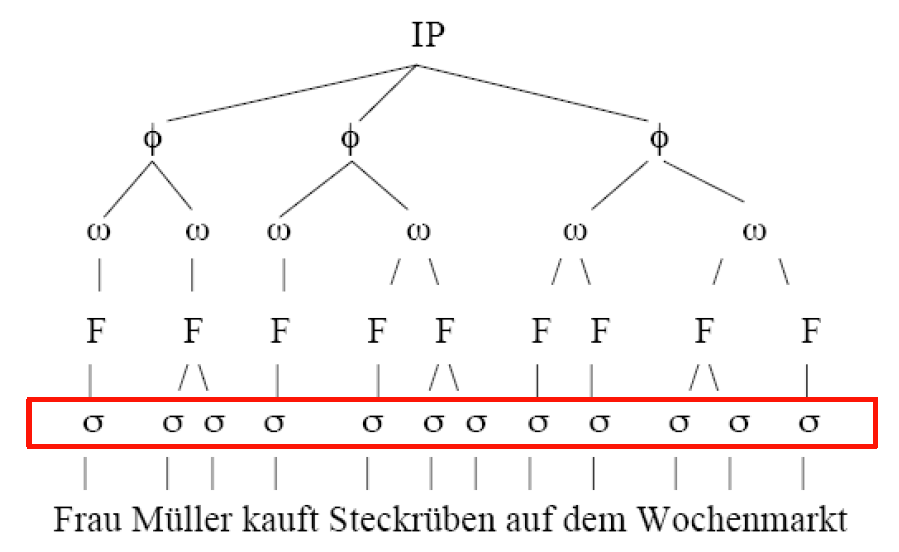
\includegraphics[scale=0.3]{material/03bHierarchieIntonationsphrase}
%	\caption{Hierarchie in der Intonationsphrase (Darstellung von C. Féry)}
%	\label{Zeichen1}
%\end{figure}

\end{frame}



%%%%%%%%%%%%%%%%%%%%%%%%%%%%%%%%%%%

\begin{frame}
\frametitle{Prosodische Konstituenten}

	\begin{multicols}{2}
	\begin{itemize}
		\item UP = Äußerungsphrase
		\item IP = Intonationsphrase
		\item $\varphi$ = phonol. Phrase
\columnbreak
		\item $\omega$ = phonol. Wort
		\item F = phonol. Fuß
		\item \alertred{$\sigma$ = Silbe}
	\end{itemize}
	\end{multicols}


	\begin{figure}
	\centering
	\scalebox{.65}{
		\begin{forest} MyP edges,
		[UP, name=up
		[IP, name=IP
		[$\varphi$[$\omega$[F[$\sigma$][$\sigma$]][F[$\sigma$][$\sigma$]]]]
		[$\varphi$, name=Phi[$\omega$[F[$\sigma$][$\sigma$]]][$\omega$, name=omega[F, name=F[$\sigma$][$\sigma$, name=sigma]]]]
		]]
		{\draw[black] (up.east)--(3,0);
			\draw[black] (IP.east)--(3,-1);
			\draw[black] (Phi.east)--(3,-2);
			\draw[black] (omega.east)--(3,-3);
			\draw[black] (F.east)--(3,-4);
			\draw[black] (sigma.east)--(3,-5.3);
			\node[right] at (3,0) {(Mandarinen oder Äpfel)\textsubscript{UP}};
			\node[right] at (3,-1) {(Mandarinen oder Äpfel)\textsubscript{IP}};
			\node[right] at (3,-2) {(Mandarinen)\textsubscript{$\varphi$} (oder Äpfel)\textsubscript{$\varphi$}};
			\node[right] at (3,-3) {(Mandarinen)\textsubscript{$\omega$} (oder)\textsubscript{$\omega$} (Äpfel)\textsubscript{$\omega$}};
			\node[right] at (3,-4) {(Manda)\textsubscript{F} (rinen)\textsubscript{F} (oder)\textsubscript{F} (Äpfel)\textsubscript{F}};
			\node[right] at (3,-5.3) {(Man)\textsubscript{$\sigma$} (da)\textsubscript{$\sigma$} (ri)\textsubscript{$\sigma$} (nen)\textsubscript{$\sigma$} (o)\textsubscript{$\sigma$} (der)\textsubscript{$\sigma$} (Äp)\textsubscript{$\sigma$} (fel)\textsubscript{$\sigma$}};
	}
		\end{forest}
	}
		\caption{\cite{Fuhrhop&Co13a}}
	\end{figure}


%\begin{figure}[b]
%	\centering
%	
%	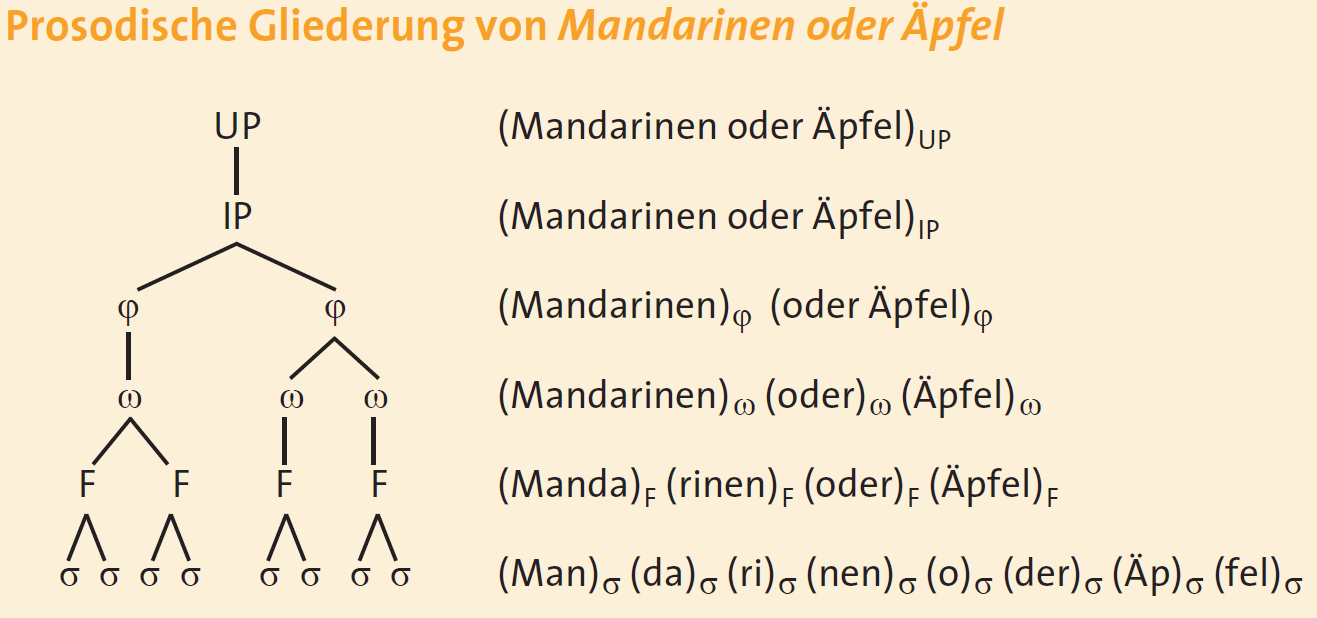
\includegraphics[scale=0.26]{material/03bHierarchieUP}
%	\caption{Hierarchie in der Äußerungsphrase \citep[8]{Fuhrhop&Co13a}}
%	%\label{Zeichen1}
%\end{figure}


\end{frame}



%%%%%%%%%%%%%%%%%%%%%%%%%%%%%%%%%%
%%%%%%%%%%%%%%%%%%%%%%%%%%%%%%%%%%
\subsection{Silbenbestimmung}
%\frame{
%\frametitle{~}
%\begin{multicols}{2}
%	\tableofcontents[currentsection]
%\end{multicols}	
%}
%%%%%%%%%%%%%%%%%%%%%%%%%%%%%%%%%%

\begin{frame}
\frametitle{Silbenbestimmung}

\begin{itemize}
	\item<1-> Wie viele Silben hat das folgende Wort?
	
	  \ea
          Silbenbestimmung
          \z
          
	
	\item<2-> Woher wissen Sie das?
	
	\begin{itemize}
		\item<2-> Staffeldt (2010: 133):\\
		\gqq{Jeder kompetente Sprachteilhaber verfügt über die \textbf{Fähigkeit},\\
 Silben identifizieren zu können.}
		
		\item<2-> \citet[600]{Bussmann02a}:\\
		\gqq{Silbe: Phonetisch-phonologische \textbf{Grundeinheit} des Wortes bzw.\ der Rede, die zwar \textbf{intuitiv} nachweisbar ist, wissenschaftlich aber \textbf{nicht einheitlich definiert} wird.}
		
	\end{itemize}

	\item<2-> Silben können \textbf{betont} werden (tragen Akzent)
	
	\item<2-> Silbenspiele
% Geheimsprache, nach Silben wird immer pi, pa, pe oder so eingesetzt
	
	\item<2-> Intuitiv erkennbare Einheit

\end{itemize}

\end{frame}



%%%%%%%%%%%%%%%%%%%%%%%%%%%%%%%%%%
%%%%%%%%%%%%%%%%%%%%%%%%%%%%%%%%%%
\subsection{Silbenstruktur}
%\frame{
%\frametitle{~}
%\begin{multicols}{2}
%	\tableofcontents[currentsection]
%\end{multicols}	
%
%}
%%%%%%%%%%%%%%%%%%%%%%%%%%%%%%%%%%
\begin{frame}
\frametitle{Silbenstruktur}

\begin{itemize}
	\item Welche Silben (des Deutschen) sind mit den folgenden Segmenten bildbar?
	
	  \ea
          \textipa{[p]}, \textipa{[a]}, \textipa{[l]}, \textipa{[t]}
          \z
\pause	
\eal
\ex Bildbar:\\
	\textipa{[palt]}, \textipa{[alpt]}, \textipa{[lapt]}, \textipa{[talp]}, \textipa{[plat]}
\ex Nicht bildbar:\\
	*\textipa{[ltap]}, \\
	*\textipa{[lpat]},\\
	*\textipa{[ptla]}, \\
	*\textipa{[tpal]}, \ldots \\
\zl
\pause
	\item Warum?
\end{itemize}

\end{frame}



%%%%%%%%%%%%%%%%%%%%%%%%%%%%%%%%%%%
%\begin{frame}
%\frametitle{Silbenstruktur}
%
%Die Silbe ist \textbf{intern strukturiert} und besteht aus den folgenden Teilen:
%
%\begin{minipage}{.60\textwidth}
%
%\begin{itemize}
%	\item[]
%	\item Silbenanlaut / Silbenanfangsrand / \alert{Onset},
%	\begin{itemize}
%		\item 0 bis $n$ Konsonanten, wobei in fast allen Sprachen $n < 5$
%	\end{itemize}
%	
%	\item[]
%	\item Silbengipfel / Silbenkern / \alert{Nukleus},
%	\begin{itemize}
%		\item Vokale
%		\item manchmal (vokalische) Nasale oder Liquide
%	\end{itemize}
%	
%	\item[]
%	\item Silbenauslaut / Silbenendrand / \alert{Koda}
%	\begin{itemize}
%		\item 0 bis $n$ Konsonanten, wobei in fast allen Sprachen $n < 5$
%	\end{itemize}
%
%	\item[]
%	\item Nukleus und Koda bilden den \alert{Reim}
%	
%\end{itemize}
%
%
%\end{minipage}
%\begin{minipage}{.39\textwidth}
%
%%%%%%%%%%%%%%
%%% Forestset Syllables

\newbox\foreststrutbox
\setbox\foreststrutbox=\hbox to 0pt{\phantom{\forestOve{standard node}{content}}}
\def\foreststrut{\copy\foreststrutbox}
\forestset{
GP1/.style 2 args={
for n={1}{baseline},
s sep=0pt, l sep=0pt,
for descendants={
l sep=0pt, l={#1},
anchor=base,calign=first,child anchor=north,
inner xsep=1pt,inner ysep=2pt,outer sep=0pt,s sep=0pt,
},
delay={
if content={}{phantom}{for children={no edge}},
for tree={
if content={O}{tier=OR}{},
if content={R}{tier=OR}{},
if content={N}{tier=N}{},
if content={x}{
tier=x,content={$\times$},outer xsep={#2},
for tree={calign=center},
for descendants={content format={\foreststrut\forestoption{content}}},
before drawing tree={outer xsep=0pt,delay={typeset node}},
s sep=4pt
}{},
},
},
before drawing tree={where content={}{parent anchor=center,child anchor=center}{}},
},
GP1/.default={5ex}{8.0pt},
associate/.style={%
tikz+={\draw(!)--(!#1);}},
spread/.style={
before drawing tree={tikz+={\draw[dotted](!)--(!#1);}}},
govern/.style={
before drawing tree={tikz+={\draw[->](!)--(!#1);}}},
p-govern/.style={
before drawing tree={tikz+={\draw[->](.north) to[out=150,in=30] (!#1.north);}}},
no p-govern/.style={
before drawing tree={tikz+={\draw[->,loosely dashed](.north) to[out=150,in=30] (!#1.north);}}},
encircle/.style={before drawing tree={circle,draw,inner sep=0pt}},
fen/.style={pin={[font=\footnotesize,inner sep=1pt,pin edge=<-]10:\textsc{Fen}}},
el/.style={content=\textsc{\textbf{##1}}},
head/.style={content=\textsc{\textbf{\underline{##1}}}},
llap/.style={
tikz+={%
\edef\forest@temp{\noexpand\node[\option{node options},
anchor=base east,at=(.base east)]}%
\forest@temp{#1\phantom{\option{environment}}};
}
},
rlap/.style={
tikz+={%
\edef\forest@temp{\noexpand\node[\option{node options},
anchor=base west,at=(.base west)]}%
\forest@temp{\phantom{\option{environment}}#1};
}
},
}
%%%%%%%%%%%%%

%\begin{figure}
%\centering
%\begin{forest} MyP edges, GP1 [
%  [$\sigma$
%    [O	[ [C$^{n}$]]
%    ]
%    [R	[N
%    		[V$^{n}$]
%    	]
%    	[K
%    		[C$^{n}$]
%    	]
%    ]
%  ]
%]
%\end{forest}
%\caption{Silbenstruktur}
%\end{figure}
%
%\end{minipage}
%
%\end{frame}



%%%%%%%%%%%%%%%%%%%%%%%%%%%%%%%%%%

\begin{frame}
\frametitle{Silbenstruktur: Komplexe Silbe}

Die Silbe ist \textbf{intern strukturiert} und besteht aus den folgenden Teilen:

\begin{minipage}{.59\textwidth}

\begin{itemize}
	\item[]
	\item \alertred{Onset}
	
	\item \alertred{Reim}
	
	\item \alertred{Nukleus}
	
	\item \alertred{Koda}
	\item[] 
	\item C $:=$ Konsonantisch, d.\,h. nicht-silbisch ($\neq$Konsonant)
	\item V $:=$ Vokalisch, d.\,h. silbisch ($\neq$Vokal)
	
\end{itemize}


\end{minipage}
\begin{minipage}{.40\textwidth}

%%%%%%%%%%%%%%
%%% Forestset Syllables

\newbox\foreststrutbox
\setbox\foreststrutbox=\hbox to 0pt{\phantom{\forestOve{standard node}{content}}}
\def\foreststrut{\copy\foreststrutbox}
\forestset{
GP1/.style 2 args={
for n={1}{baseline},
s sep=0pt, l sep=0pt,
for descendants={
l sep=0pt, l={#1},
anchor=base,calign=first,child anchor=north,
inner xsep=1pt,inner ysep=2pt,outer sep=0pt,s sep=0pt,
},
delay={
if content={}{phantom}{for children={no edge}},
for tree={
if content={O}{tier=OR}{},
if content={R}{tier=OR}{},
if content={N}{tier=N}{},
if content={x}{
tier=x,content={$\times$},outer xsep={#2},
for tree={calign=center},
for descendants={content format={\foreststrut\forestoption{content}}},
before drawing tree={outer xsep=0pt,delay={typeset node}},
s sep=4pt
}{},
},
},
before drawing tree={where content={}{parent anchor=center,child anchor=center}{}},
},
GP1/.default={5ex}{8.0pt},
associate/.style={%
tikz+={\draw(!)--(!#1);}},
spread/.style={
before drawing tree={tikz+={\draw[dotted](!)--(!#1);}}},
govern/.style={
before drawing tree={tikz+={\draw[->](!)--(!#1);}}},
p-govern/.style={
before drawing tree={tikz+={\draw[->](.north) to[out=150,in=30] (!#1.north);}}},
no p-govern/.style={
before drawing tree={tikz+={\draw[->,loosely dashed](.north) to[out=150,in=30] (!#1.north);}}},
encircle/.style={before drawing tree={circle,draw,inner sep=0pt}},
fen/.style={pin={[font=\footnotesize,inner sep=1pt,pin edge=<-]10:\textsc{Fen}}},
el/.style={content=\textsc{\textbf{##1}}},
head/.style={content=\textsc{\textbf{\underline{##1}}}},
llap/.style={
tikz+={%
\edef\forest@temp{\noexpand\node[\option{node options},
anchor=base east,at=(.base east)]}%
\forest@temp{#1\phantom{\option{environment}}};
}
},
rlap/.style={
tikz+={%
\edef\forest@temp{\noexpand\node[\option{node options},
anchor=base west,at=(.base west)]}%
\forest@temp{\phantom{\option{environment}}#1};
}
},
}
%%%%%%%%%%%%%


\begin{figure}
\centering
\begin{forest} MyP edges, GP1 [
  [$\sigma$
    [O
    	[[C[\textipa{S}]]]
    	[[C[\textipa{t}]]]
    	[[C[\textipa{\textscr}]]]
    ]
    [R
    	[N
    		[V[\textipa{U}]]
    	]
    	[K
    		[C[\textipa{m}]]
    		[C[\textipa{\t{pf}}]]
    		[C[\textipa{s}]]
    		[C[\textipa{t}]]
    	]
    ]
  ]
]
\end{forest}
%\caption{Komplexe Silbe}
\end{figure}
% wahrscheinlich komplexeste Koda, die es gibt.
\end{minipage}

\end{frame}



%%%%%%%%%%%%%%%%%%%%%%%%%%%%%%%%%%
\begin{frame}
\frametitle{Silbenstruktur: Minimale Silbe}

Die Silbe ist \textbf{intern strukturiert} und besteht aus den folgenden Teilen:

\begin{minipage}{.60\textwidth}

\begin{itemize}
	\item[]
	\item \alertred{Onset}
	
	\item \alertred{Reim}
	
	\item \alertred{Nukleus}
	
	\item \alertred{Koda}
	\item[] 
	\item \textbf{Minimale Silbe} besteht nur aus einem V im  Nukleus
	  \ea
          \ab{gehe} \ras \textipa{[ge:.@]}
          \z
	
\end{itemize}


\end{minipage}
\begin{minipage}{.39\textwidth}

%%%%%%%%%%%%%%
%%% Forestset Syllables

\newbox\foreststrutbox
\setbox\foreststrutbox=\hbox to 0pt{\phantom{\forestOve{standard node}{content}}}
\def\foreststrut{\copy\foreststrutbox}
\forestset{
GP1/.style 2 args={
for n={1}{baseline},
s sep=0pt, l sep=0pt,
for descendants={
l sep=0pt, l={#1},
anchor=base,calign=first,child anchor=north,
inner xsep=1pt,inner ysep=2pt,outer sep=0pt,s sep=0pt,
},
delay={
if content={}{phantom}{for children={no edge}},
for tree={
if content={O}{tier=OR}{},
if content={R}{tier=OR}{},
if content={N}{tier=N}{},
if content={x}{
tier=x,content={$\times$},outer xsep={#2},
for tree={calign=center},
for descendants={content format={\foreststrut\forestoption{content}}},
before drawing tree={outer xsep=0pt,delay={typeset node}},
s sep=4pt
}{},
},
},
before drawing tree={where content={}{parent anchor=center,child anchor=center}{}},
},
GP1/.default={5ex}{8.0pt},
associate/.style={%
tikz+={\draw(!)--(!#1);}},
spread/.style={
before drawing tree={tikz+={\draw[dotted](!)--(!#1);}}},
govern/.style={
before drawing tree={tikz+={\draw[->](!)--(!#1);}}},
p-govern/.style={
before drawing tree={tikz+={\draw[->](.north) to[out=150,in=30] (!#1.north);}}},
no p-govern/.style={
before drawing tree={tikz+={\draw[->,loosely dashed](.north) to[out=150,in=30] (!#1.north);}}},
encircle/.style={before drawing tree={circle,draw,inner sep=0pt}},
fen/.style={pin={[font=\footnotesize,inner sep=1pt,pin edge=<-]10:\textsc{Fen}}},
el/.style={content=\textsc{\textbf{##1}}},
head/.style={content=\textsc{\textbf{\underline{##1}}}},
llap/.style={
tikz+={%
\edef\forest@temp{\noexpand\node[\option{node options},
anchor=base east,at=(.base east)]}%
\forest@temp{#1\phantom{\option{environment}}};
}
},
rlap/.style={
tikz+={%
\edef\forest@temp{\noexpand\node[\option{node options},
anchor=base west,at=(.base west)]}%
\forest@temp{\phantom{\option{environment}}#1};
}
},
}
%%%%%%%%%%%%%


\begin{figure}
\centering
\begin{forest} MyP edges, GP1 [
  [$\sigma$
    [O
    ]
    [R
    	[N
    		[V[\textipa{@}]]
    	]
    	[K
    	]
    ]
  ]
]
\end{forest}
%\caption{Minimale Silbe}
\end{figure}


\end{minipage}

\end{frame}

%%%%%%%%%%%%%%%%%%%%%%%%%%%%%%%%%%
\begin{frame}
\frametitle{Offene/geschlossene/nackte/bedeckte Silben}

\begin{itemize}
	\item Silbenanlaut/Silbenanfangsrand/\alertred{Onset},
	\item Silbengipfel/Silbenkern/\alertred{Nukleus},
	\item Silbenauslaut/Silbenendrand/\alertred{Koda}
	
\end{itemize}

\begin{table}
\centering
\begin{tabular}{lllll}
\textsc{Onset} & \textsc{Nukleus} & \textsc{Koda} & \textsc{Term} & \textsc{Merkmal} \\
\hline
\textipa{z} & \textipa{e:} & & Offene Silbe & Koda leer\\
\hline
\textipa{t} & \textipa{a:} & \textipa{l} & Geschlossene Silbe & Koda besetzt\\
\hline
 & \textipa{@} & \textipa{n} & Nackte Silbe & Onset leer\\
\hline
\textipa{z} & \textipa{e:} & & Bedeckte Silbe & Onset besetzt\\
\end{tabular}
\end{table}

\end{frame}



%%%%%%%%%%%%%%%%%%%%%%%%%%%%%%%%%%
%%%%%%%%%%%%%%%%%%%%%%%%%%%%%%%%%%
%\subsubsection{Onset}
%\frame{
%\begin{multicols}{2}
%\frametitle{~}
%	\tableofcontents[currentsection]
%\end{multicols}
%}
%%%%%%%%%%%%%%%%%%%%%%%%%%%%%%%%%%

\begin{frame}
\frametitle{Onset}

\begin{multicols}{2}
Sprachbeispiele:
	
\ea
Tschechisch \textipa{[fspla.nout]} \gq{aufflammen}
\z

\ea
Hawaianisch \textipa{[a.lo.ha]} \gq{Liebe}
\z

\ea
Deutsch \textipa{[St\textscr aIt]} \gq{Streit}
\z

Im Deutschen sind
	\begin{itemize}
		\item \textbf{3 Cs} beschränkt möglich (nach \textipa{/S/} und \textipa{/s/}),

% 3 = Streit, häfiger 2
		
		\item \textbf{2 Cs} oft (\zB \textipa{/bl/}, \textipa{/kn/} \ldots\ ), und
		\item \textbf{1 C} immer (bis auf \textipa{[N]})
	\end{itemize}

\columnbreak

\begin{table}
\centering

\begin{tabular}{c|c|c|c|c}
 & \textipa{m} & \textipa{n} & \textipa{l} & \textipa{\textscr} \\ 
\hline 
\textipa{p} &  &  & + & + \\ 
\hline 
\textipa{b} &  &  & + & + \\ 
\hline 
\textipa{t} &  &  &  & + \\ 
\hline 
\textipa{d} &  &  &  & + \\ 
\hline 
\textipa{k} &  & + & + & + \\ 
\hline 
\textipa{g} &  & + & + & + \\ 
\hline 
\textipa{f} &  &  & + & + \\
\hline 
\textipa{v} &  &  &  & + \\ 
\hline 
\textipa{S} & + & + & + & + \\ 
\end{tabular} 

\caption{Kombinatorik}
\end{table}

\end{multicols}

\end{frame}



%%%%%%%%%%%%%%%%%%%%%%%%%%%%%%%%%%

\begin{frame}
\frametitle{Onset: Silbenanlautgesetz}

\begin{itemize}
	\item Bei Betrachtung aller (bekannten) Sprachen kann man die folgende Gesetzmäßigkeit feststellen \citep[cf.][212f.]{Hall00a}
	
	\begin{block}{Silbenanlautgesetz}
	
	\sub{$\sigma$}[CV $>$ \sub{$\sigma$}[V 
	und
	\sub{$\sigma$}[C\MyPup{$n$}V $>$ \sub{$\sigma$}[C\MyPup{$n+1$}V \\
	$>$ $:=$ häufiger als oder ist weniger markiert als 

% Silbe mit Konsonant und Vokal sind häfiger als solche, die nur mit Vokal beginnen
% Silbe mit n Konsonanten ist weniger markiert als Silbe mit n+1 KOnsonanten.


	
	\end{block}
	 
	 \item Man spricht auch von der Markiertheit von Silben,\\
               wenn sie Präferenzgesetzen widersprechen.

\end{itemize}

\end{frame}



%%%%%%%%%%%%%%%%%%%%%%%%%%%%%%%%%%
%%%%%%%%%%%%%%%%%%%%%%%%%%%%%%%%%%
%\subsubsection{Nukleus}
%\frame{
%\begin{multicols}{2}
%\frametitle{~}
%	\tableofcontents[currentsection]
%\end{multicols}
%}
%%%%%%%%%%%%%%%%%%%%%%%%%%%%%%%%%%

\begin{frame}
\frametitle{Nukleus: Silbenkerngesetz}

\begin{itemize}

	\item In allen Sprachen werden Nuklei durch \textbf{Vokale} (V) gebildet
	
	\item In einigen Sprachen können Nuklei auch durch \textbf{Liquide und Nasale} (C \ras V) gebildet werden


	
	\item Im Deutschen werden bei schnellem Sprechen folgende Wörter mit so genannten \textbf{silbischen Konsonanten} gesprochen
	
	
          \ea
          \ab{lesen} \textipa{[le:.z\textsyllabic{n}]} %
          \z
          
          \ea
          \ab{Wandel} \textipa{[van.d\textsyllabic{l}]}
          \z

	\item Bei Betrachtung aller (bekannten) Sprachen kann man die folgende Gesetzmäßigkeit feststellen \citep[cf.][217f.]{Hall00a}

\end{itemize}
	
	\begin{block}{Silbenkerngesetz}
	
	Silben mit einfachem vokalischem Nukleus sind universell bevorzugt.
	
	Vokale $>$ Sonoranten $>$ Obstruenten 
	
	\end{block}
	
\end{frame}



%%%%%%%%%%%%%%%%%%%%%%%%%%%%%%%%%%
%%%%%%%%%%%%%%%%%%%%%%%%%%%%%%%%%%
%\subsubsection{Koda}
%\frame{
%\begin{multicols}{2}
%\frametitle{~}
%	\tableofcontents[currentsection]
%\end{multicols}
%}
%%%%%%%%%%%%%%%%%%%%%%%%%%%%%%%%%%

\begin{frame}
\frametitle{Koda: Silbenauslautgesetz}

In der Koda sind/ist \ldots

\begin{itemize}

	\item \ldots\ in \emph{vielen} Sprachen keine Konsonanten erlaubt (\zB Hawaiianisch),
	
	\item \ldots\ in \emph{einigen} Sprachen ein Konsonant erlaubt,
	
	\item \ldots\ in \emph{einigen (wenigen)} Sprachen mehrere Konsonanten erlaubt.
	
	\item[]
	\item Deutsch: \textipa{[hE\textscr psts]} (0 bis 4/5 Konsonanten)
	
	\item Reihenfolge der Konsonanten unterliegt dem  \textbf{Sonoritätsprinzip}
	
	\item Bei Betrachtung aller (bekannten) Sprachen kann man die folgende Gesetzmäßigkeit feststellen \citep[cf.][214]{Hall00a}

\end{itemize}
	
	\begin{block}{Silbenauslautgesetz}
	
	CVC$^{n}$]$_{\sigma}$ $>$ CVC$^{n+1}$]$_{\sigma}$
	
	\end{block}
	
\end{frame}



%%%%%%%%%%%%%%%%%%%%%%%%%%%%%%%%%%%
%%%%%%%%%%%%%%%%%%%%%%%%%%%%%%%%%%%
\subsection{Phonotaktik}
\iftoggle{toc}{
\frame{
\frametitle{~}
\begin{multicols}{2}
	\tableofcontents[currentsection]
\end{multicols}	
}
}
%%%%%%%%%%%%%%%%%%%%%%%%%%%%%%%%%%

\begin{frame}
\frametitle{Phonotaktik}

\begin{block}{Phonotaktik}

Die Phonotaktik untersucht die syntagmatischen Beziehungen zwischen Lauten innerhalb der Silbe und anderer prosodischer Einheiten \citep{Fuhrhop&Co13a}

\end{block}

\begin{itemize}
	\item Mögliche und unmögliche Kombinationen von Segmenten bzgl.
	
	\begin{itemize}
		\item Anzahl der Laute,
		\item Art,
		\item Reihenfolge der Laute
	\end{itemize}

\end{itemize}

\end{frame}



%%%%%%%%%%%%%%%%%%%%%%%%%%%%%%%%%%%
%%%%%%%%%%%%%%%%%%%%%%%%%%%%%%%%%%%
%\subsubsection{Sonoritätshierarchie}
%\frame{
%\begin{multicols}{2}
%\frametitle{~}
%	\tableofcontents[currentsection]
%\end{multicols}
%}
%%%%%%%%%%%%%%%%%%%%%%%%%%%%%%%%%%

\begin{frame}
\frametitle{Sonoritätshierarchie}

\begin{itemize}
	\item Betrachten Sie die folgenden Beispiele und überlegen Sie \ldots
	
	\begin{enumerate}
		\item \ldots\ welche \textbf{phonotaktischen Beschränkungen} für den Onset in deutschen Silben gelten könnten:

                  \ea
                  \textipa{[\textcolor{red}{k\textscr}aNk]}, \textipa{[\textcolor{red}{pl}a:n]}, \textipa{[\textcolor{red}{f\textscr}E\c{c}]},
                  \textipa{[\textcolor{red}{fl}o:]}, \textipa{[\textcolor{red}{kn}i:]}, \textipa{[\textcolor{red}{gn}a:d@]}
                  \z

                  \ea
                  *\textipa{[\textcolor{red}{{\textscr}k}aNk]}, *\textipa{[\textcolor{red}{lp}a:n]}, *\textipa{[\textcolor{red}{{\textscr}f}E\c{c}]}, *\textipa{[\textcolor{red}{lf}o:]}, *\textipa{[\textcolor{red}{nk}i:]}, *\textipa{[\textcolor{red}{ng}a:d@]}
                  \z
                  
\pause
		\item \ldots\ welche \textbf{phonotaktischen Beschränkungen} für die Koda in deutschen Silben gelten könnten:

                  \ea
                  \textipa{[ka\textcolor{red}{lt}]}, \textipa{[ha\textcolor{red}{{\textscr}t}]}, \textipa{[la\textcolor{red}{nt}]}, \textipa{[k{\textscr}a\textcolor{red}{Nk}]}
                  \z

                  \ea
                  *\textipa{[ka{tl}]}, *\textipa{[ha{t\textscr}]}, *\textipa{[la\textcolor{red}{tn}]},
                  *\textipa{[k\textscr a\textcolor{red}{kN}]}
                  \z

	\end{enumerate}
	
\end{itemize}

\end{frame}



%%%%%%%%%%%%%%%%%%%%%%%%%%%%%%%%%%
\begin{frame}
%\frametitle{Sonoritätshierarchie}

\begin{enumerate}
	\item \textbf{phonotaktischen Beschränkungen} \ras Onset
	
          \ea
          \textipa{[k\textscr aNk]}, \textipa{[pla:n]}, \textipa{[f\textscr E\c{c}]},
          \textipa{[flo:]}, \textipa{[kni:]}, \textipa{[gna:d@]}
          \z

          \ea
          *\textipa{[lbat]}, *\textipa{[\textscr to:k]}, *\textipa{[nki:l]}, *\textipa{[ngak]}
          \z

	\item \textbf{phonotaktischen Beschränkungen} \ras Koda

          \ea
          \textipa{[kalt]}, \textipa{[ha5t]}, \textipa{[lant]}, \textipa{[k\textscr aNk]}
          \z

          \ea
          *\textipa{[katl]}, *\textipa{[hat\textscr ]}, *\textipa{[latn]}, *\textipa{[k\textscr
              akN]}
          \z

\end{enumerate}
	

\begin{table}
\centering
\begin{tabular}{c|c|c|c|c} 
 & Sonorant & Obstruent & Vokal & Laryngal \\ 
\hline 
[kon] & $[+]$ & $[+]$ & $[-]$ & $[-]$ \\ 
\hline 
[son] & $[+]$ & $[-]$ & $[+]$ & $[-]$
\end{tabular} 

\end{table}

\begin{itemize}
	\item \textbf{Onset}: Obstruent vor Sonorant
	\item \textbf{Koda}: Sonorant vor Obstruent
\end{itemize}

\end{frame}



%%%%%%%%%%%%%%%%%%%%%%%%%%%%%%%%%%

\begin{frame}
%\frametitle{Sonoritätshierarchie}

\begin{itemize}
	\item Eine Silbe ist so aufgebaut, dass die Sonorität in der Silbe zum Nukleus hin steigt und dann abfällt.

	\item \textbf{Sonorität} $:=$ Schallfülle, Intensität

\end{itemize}

\begin{figure}
\centering
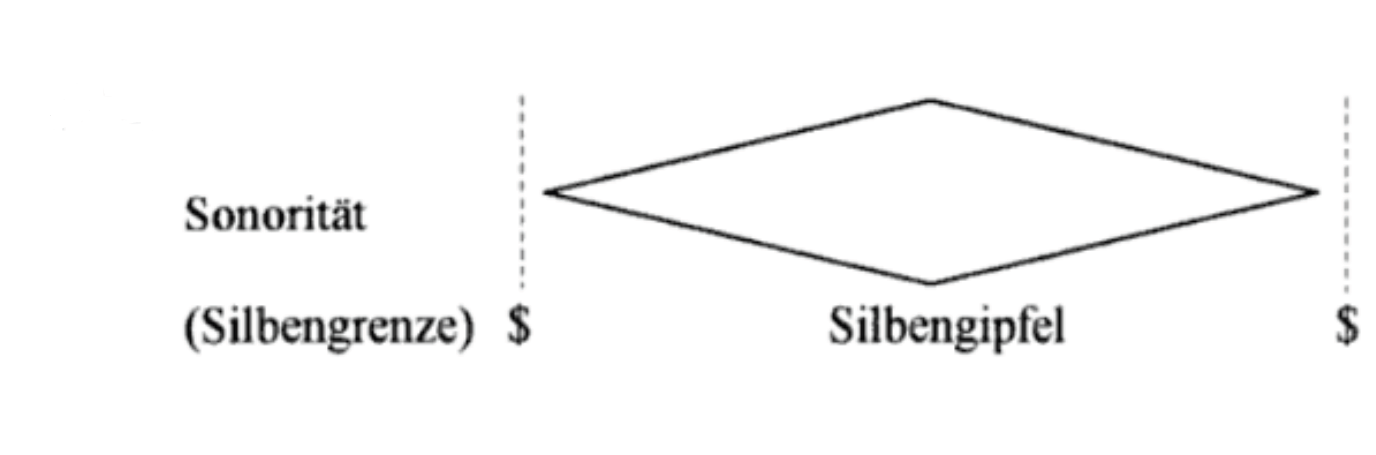
\includegraphics[scale=.2]{material/03bSonoritaetRamers}
\caption{Nach \citet[93]{Ramers08a} (apud Lenerz 1985)}
\end{figure}
% Vokale sind sonorste Elemente
% m > p

% s > p  (frikativ > plosiv)

\begin{itemize}
	\item Laute können nach der Sonoritätshierarchie auf einer Skala (nach ihrer \textbf{Sonorität}) angeordnet werden.
\end{itemize}

\end{frame}



%%%%%%%%%%%%%%%%%%%%%%%%%%%%%%%%%%

\begin{frame}
%\frametitle{Sonoritätshierarchie}

\begin{itemize}
	\item Es gibt verschiedene Ausformulierungen der Sonoritätshierachie.

\end{itemize}

\begin{table}
\centering
\begin{tabular}{l|l|l|l|l} 
	 & einfach 				  	 & Hall 					  & \textbf{Wiese} 				& komplex  \\ 
\hline
\hline 
$[+]$& \multirow{6}{*}{Sonorant} & \multirow{2}{*}{Vokal} 	  & \multirow{2}{*}{Vokal} 		& Vokal  \\ 
	 & 							 & 						 	  &								& Vokal (hoch) \\
\cline{3-5}			
	 &							 & \multirow{3}{*}{Liquide}   &								& Gleitlaut \\
	 &						  	 &	 						  & \textipa{/\textscr /}		& Vibrant \\
\cline{4-5}			
	 &						 	 &							  & \textipa{/l/}				& Lateral \\
\cline{3-5}			
	 &							 & Nasal					  & Nasal						& Nasal \\
\hline			
	 &\multirow{6}{*}{Obstruent} & \multirow{6}{*}{Obstruent} & \multirow{3}{*}{Frikativ}	& $[+$sth$]$ Frikativ \\
	 &						 	 &							  &								& $[+$sth$]$ Affrikat \\		
	 &							 &							  &								& $[+$sth$]$ Plosiv \\
\cline{4-5}			
	 &						  	 &							  & \multirow{3}{*}{Plosiv}		& $[-$sth$]$ Frikativ \\
	 &						 	 &							  &								& $[-$sth$]$ Affrikat \\		
$[-]$&							 &							  &								& $[-$sth$]$ Plosiv \\
		
\end{tabular} 

\end{table}

\end{frame}



%%%%%%%%%%%%%%%%%%%%%%%%%%%%%%%%%%

\begin{frame}
%\frametitle{Sonoritätshierarchie}


\begin{block}{Sonoritätsprinzip (Sonority Sequencing Generalization -- SSG)}
In jeder Silbe gibt es ein Segment, das den Silbengipfel bildet, und dem ein oder mehrere Segmente vorangehen und/oder folgen, deren Sonoritätswerte zum Silbengipfel hin zunehmen und danach abnehmen. (vgl. \citealt[225]{Hall00a}, \citealt[94]{Ramers08a})
\end{block}

\begin{itemize}
	\item Strikt: Monoton steigend oder fallend
	\item Abgeschwächt: auch gleichbleibend \citep[vgl.][]{Hall00a}

\end{itemize}

\begin{figure}
\centering
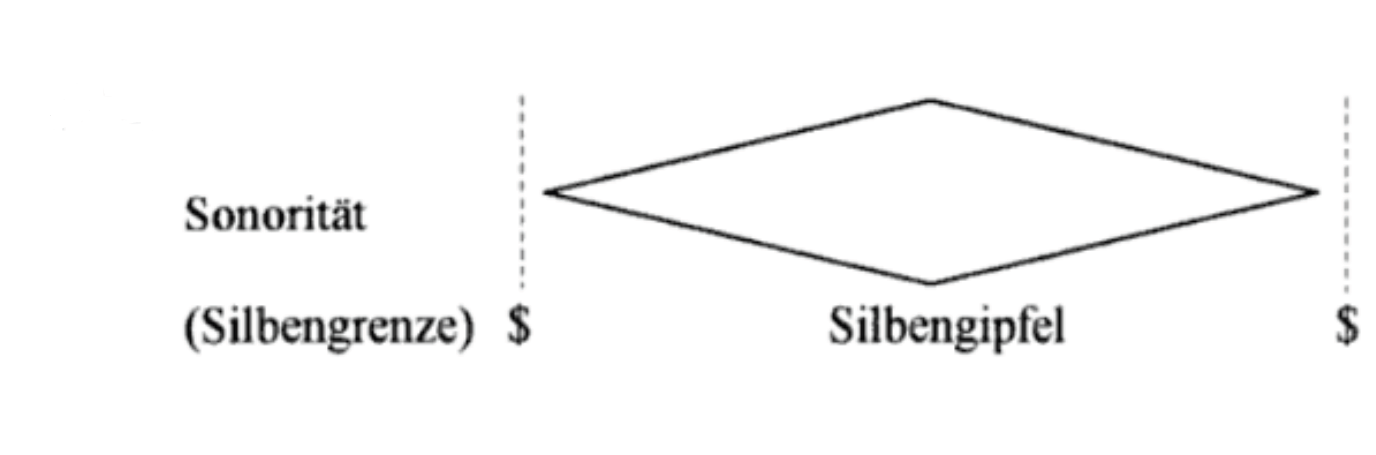
\includegraphics[scale=.2]{material/03bSonoritaetRamers}
\caption{Nach \citet[93]{Ramers08a} (apud Lenerz 1985)}
\end{figure}

\end{frame}



%%%%%%%%%%%%%%%%%%%%%%%%%%%%%%%%%%

\begin{frame}
%\frametitle{Sonoritätshierarchie}

\begin{block}{Sonoritätshierarchie (für uns)}
Vokal $>$ \textipa{/\textscr /} $>$ \textipa{/l/} $>$ Nasal $>$ Frikativ $>$ Plosiv \\
$x > y$ $:=$ $x$ ist sonorer als $y$
\end{block}

\begin{figure}
	\centering
	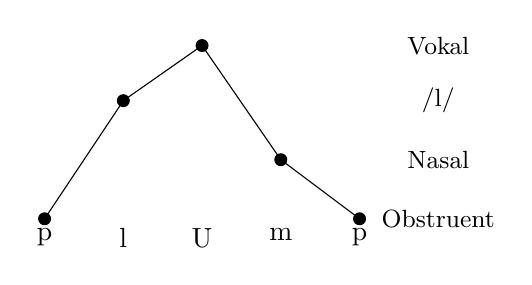
\begin{tikzpicture}
	\draw[fill] (0,0) circle [radius=0.075];
	\draw[black] (0,0)--(1,1.5);
	\draw[fill] (1,1.5) circle [radius=0.075];
	\draw[black] (1,1.5)--(2,2.2);
	\draw[fill] (2,2.2) circle [radius=0.075];
	\draw[black] (2,2.2)--(3,0.75);
	\draw[fill] (3,0.75) circle [radius=0.075];
	\draw[black] (3,0.75)--(4,0);
	\draw[fill] (4,0) circle [radius=0.075];
	\node[below] at (0,0){p};
	\node[below] at (1,0){l};
	\node[below] at (2,0){\textipa{U}};
	\node[below] at (3,0){m};
	\node[below] at (4,0){p};
	\node at (5,2.2){{\small Vokal}};
	\node at (5,1.5){{\small /l/}};
	\node at (5,0.75){{\small Nasal}};
	\node at (5,0){{\small Obstruent}};
\end{tikzpicture}
\caption{\citet[225]{Hall00a}}
\end{figure}


%\begin{figure}
%\centering
%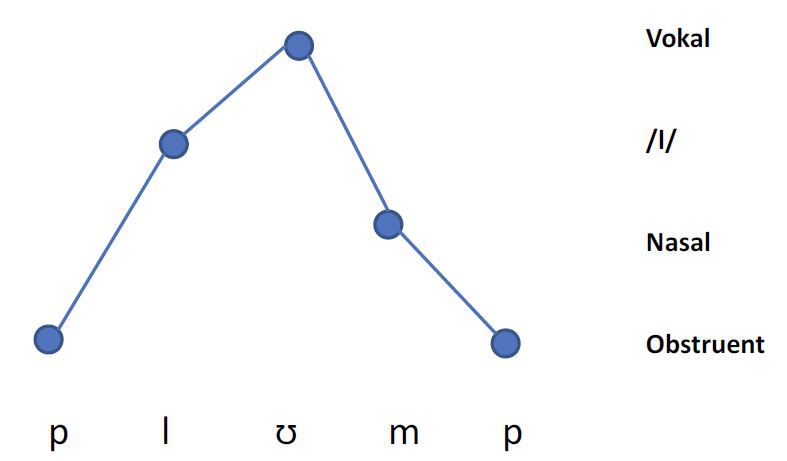
\includegraphics[scale=.3]{material/03bSonoritaetBsp}
%\caption{\citet[225]{Hall00a}}
%\end{figure}

\begin{itemize}
	\item Sonoritätshierarchie wird je nach Sprache leicht anders spezifiziert.
\end{itemize}
\end{frame}


\iftoggle{uebung}{
%%%%%%%%%%%%%%%%%%%%%%%%%%%%%%%%%%
\begin{frame}
\frametitle{Übung}

\begin{itemize}
	\item Geben Sie die Sonoritätsprofile der folgenden Silben an.
	
	  \ea
          Spatz, Dachs, Clown, Milch
          \z

% bei Spatz geht es von Frikativ s auf Plosiv p runter = Ausnahme
% bei Dachs geht es auf k runter und dann auf s hoch   = Ausnahme
% clown k = plosiv, l = /l/ au = Vokal, n = , keine Ausnahme

% Glottal stop gehört zu den Plosiven

	\item Erklären Sie die Ungramatikalität der folgenden Silben:
	
	  \ea
          *\textipa{[lbat]}, *\textipa{[blabl]}, *\textipa{[m{\textscr}apt]}, *\textipa{[ki:l\textscr]}, *\textipa{[ngang]}
          \z

% hier Probleme im Onset
% l sonorer als b


	\ea *\textipa{[krafm]}, *\textipa{[elat]}, *\textipa{[plaml]}, *\textipa{[nfatl]}

% hier auch Probleme in der Koda

        \z

\end{itemize}

\end{frame}
}

\iftoggle{loesung}{
	\begin{frame}
\frametitle{Lösung}

\begin{minipage}{.4\textwidth}
		\begin{figure}
		\centering
		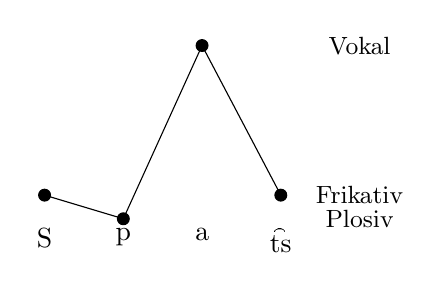
\begin{tikzpicture}
		\draw[fill] (0,0.3) circle [radius=0.075];
		\draw[black] (0,0.3)--(1,0);
		\draw[fill] (1,0) circle [radius=0.075];
		\draw[black] (1,0)--(2,2.2);
		\draw[fill] (2,2.2) circle [radius=0.075];
		\draw[black] (2,2.2)--(3,0.3);
		\draw[fill] (3,0.3) circle [radius=0.075];
		\node[below] at (0,0){\textipa{S}};
		\node[below] at (1,0){\textipa{p}};
		\node[below] at (2,0){\textipa{a}};
		\node[below] at (3,0){\textipa{\t{ts}}};
		\node at (4,0.3){{\small Frikativ}};
		\node at (4,0){{\small Plosiv}};
		\node at (4,2.2){{\small Vokal}};
		\end{tikzpicture}
	\end{figure}
\end{minipage}
\begin{minipage}{.1\textwidth}
	\hfill
\end{minipage}
\begin{minipage}{.4\textwidth}
		\begin{figure}
		\centering
		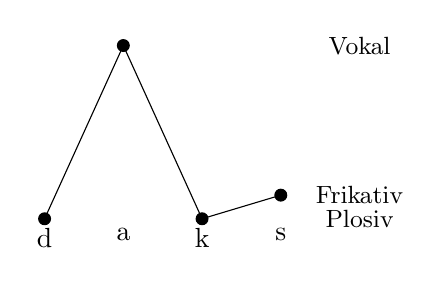
\begin{tikzpicture}
		\draw[fill] (0,0) circle [radius=0.075];
		\draw[black] (0,0)--(1,2.2);
		\draw[fill] (1,2.2) circle [radius=0.075];
		\draw[black] (1,2.2)--(2,0);
		\draw[fill] (2,0) circle [radius=0.075];
		\draw[black] (2,0)--(3,0.3);
		\draw[fill] (3,0.3) circle [radius=0.075];
		\node[below] at (0,0){\textipa{d}};
		\node[below] at (1,0){\textipa{a}};
		\node[below] at (2,0){\textipa{k}};
		\node[below] at (3,0){\textipa{s}};
		\node at (4,0.3){{\small Frikativ}};
		\node at (4,0){{\small Plosiv}};
		\node at (4,2.2){{\small Vokal}};
		\end{tikzpicture}
	\end{figure}
\end{minipage}

\begin{minipage}{.4\textwidth}
	\begin{figure}
		\centering
		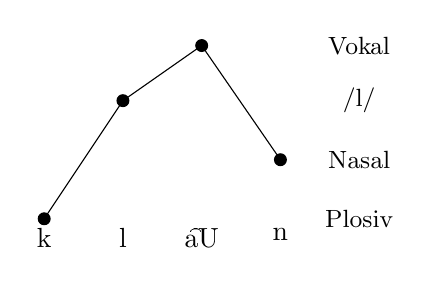
\begin{tikzpicture}
		\draw[fill] (0,0) circle [radius=0.075];
		\draw[black] (0,0)--(1,1.5);
		\draw[fill] (1,1.5) circle [radius=0.075];
		\draw[black] (1,1.5)--(2,2.2);
		\draw[fill] (2,2.2) circle [radius=0.075];
		\draw[black] (2,2.2)--(3,0.75);
		\draw[fill] (3,0.75) circle [radius=0.075];
		\node[below] at (0,0){\textipa{k}};
		\node[below] at (1,0){\textipa{l}};
		\node[below] at (2,0){\textipa{\t{aU}}};
		\node[below] at (3,0){\textipa{n}};
		\node at (4,1.5){{\small /l/}};
		\node at (4,0){{\small Plosiv}};
		\node at (4,2.2){{\small Vokal}};
		\node at (4,0.75){{\small Nasal}};
		\end{tikzpicture}
	\end{figure}
\end{minipage}
\begin{minipage}{.1\textwidth}
	\hfill
\end{minipage}
\begin{minipage}{.4\textwidth}
	\begin{figure}
		\centering
		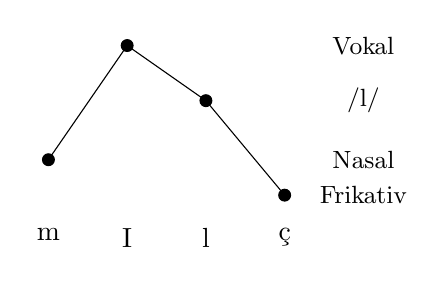
\begin{tikzpicture}
		\draw[fill] (0,0.75) circle [radius=0.075];
		\draw[black] (0,0.75)--(1,2.2);
		\draw[fill] (1,2.2) circle [radius=0.075];
		\draw[black] (1,2.2)--(2,1.5);
		\draw[fill] (2,1.5) circle [radius=0.075];
		\draw[black] (2,1.5)--(3,0.3);
		\draw[fill] (3,0.3) circle [radius=0.075];
		\node[below] at (0,0){\textipa{m}};
		\node[below] at (1,0){\textipa{I}};
		\node[below] at (2,0){\textipa{l}};
		\node[below] at (3,0){\textipa{\c{c}}};
		\node at (4,0.3){{\small Frikativ}};
		\node at (4,1.5){{\small /l/}};
		\node at (4,2.2){{\small Vokal}};
		\node at (4, 0.75){\small Nasal};
		\end{tikzpicture}
	\end{figure}
\end{minipage}

\end{frame}

\begin{frame}
	\frametitle{Lösung}
	\begin{itemize}
		\item \textipa{[bla\textcolor{red}{bl}]} \ras + Auslautverhärtung
		\item \textipa{[\textcolor{red}{ng}a\textcolor{red}{ng}]} \ras + Regressive velare Nasalassimilation + g-Tilgung
		\item \textipa{[\textcolor{red}{el}at]} \ras + Knacklauteinsetzung
	\end{itemize}
\end{frame}
}
%%%%%%%%%%%%%%%%%%%%%%%%%%%%%%%%%%
%%%%%%%%%%%%%%%%%%%%%%%%%%%%%%%%%%
%\subsubsection{Weitere phonotaktische Beschränkungen}
%\frame{
%\frametitle{~}
%\begin{multicols}{2}
%	\tableofcontents[currentsection]
%\end{multicols}	
%}
%%%%%%%%%%%%%%%%%%%%%%%%%%%%%%%%%%

\begin{frame}
\frametitle{Weitere phonotaktische Beschränkungen}

\begin{itemize}
	\item Im \textbf{Onset} in deutschen Silben können stehen:

	\begin{itemize}
		\item alle Einzelkonsonanten des Deutschen,
		\item außer \textipa{[s]} vor V, und \textipa{[N]}
		\item[]
		\item bestimmte zwei- und dreigliedrige Konsonantencluster (nach Sonoritätshierarchie)
	\end{itemize}
	
	\item[]

	\item Silben können auch \textbf{mit unbetontem Vokal} beginnen.

	\begin{itemize}
		\item Dann ist der Onset leer.
		  \ea
                  \textipa{[\textprimstress P\t{aɪ}.5]} (Eier)
                  \z

		  \ea
                  \textipa{[PEt.\textprimstress va:.I\c{c}]} (etwaig)
                  \z
	
	\end{itemize}
	
	\item Vor betontem Vokal steht immer der \textbf{Glottisschlag}.

	  \ea
          \textipa{[ka.\textprimstress Po:.tIS]}
          \z

\end{itemize}

\end{frame}



%%%%%%%%%%%%%%%%%%%%%%%%%%%%%%%%%%
%%%%%%%%%%%%%%%%%%%%%%%%%%%%%%%%%%
\subsection{Silbenmodelle}
\iftoggle{toc}{
\frame{
\frametitle{~}
\begin{multicols}{2}
	\tableofcontents[currentsection]
\end{multicols}	
}
}
%%%%%%%%%%%%%%%%%%%%%%%%%%%%%%%%%%

\begin{frame}
\frametitle{Silbenmodelle}

\begin{itemize}
	\item Bisher (hauptsächlich) nur \textbf{lineare Betrachtung} mit allen Segmenten auf einer Schicht
	  \ea
          \textipa{/pe:.t@\textscr /} (Peter)
          \z
	
	  \ea
          \textipa{/vE\.t@\textscr /} (Vetter)
          \z

	\item \textbf{Nicht-lineare Phonologie} (Autosegmentale Phonologie)
	
	\begin{itemize}
		\item verschiedene Repräsentationsebenen bzw. Schichten
		
		\item hierarchische Strukturierung
		
		\item Vorteil: Beschreibung von \textbf{Merkmalsausbreitung} und \textbf{segmentunabhängigen Prozessen}
		
	\end{itemize}
\end{itemize}

\end{frame}



%%%%%%%%%%%%%%%%%%%%%%%%%%%%%%%%%%
%%%%%%%%%%%%%%%%%%%%%%%%%%%%%%%%%%
%\subsubsection{CV-Modell}
%\frame{
%\frametitle{~}
%	\tableofcontents[currentsection]
%}


%%%%%%%%%%%%%%%%%%%%%%%%%%%%%%%%%%
\begin{frame}
\frametitle{CV-Modell (Einfaches Modell)}

\begin{itemize}
	\item Silben und Segmente auf unterschiedlichen Schichten
		
	\item Verbunden durch Assoziationslinien
		
	\item Charakterisierung der Silbenstruktur durch C und V 
\end{itemize}


\begin{figure}
\centering
\begin{forest}
MyP edges,
[$\sigma$
	[C [\textipa{b}]]
	[C [\textipa{l}]]
	[V [\textipa{I}]]
	[C [\textipa{n}]]
	[C [\textipa{t}]]
]
\end{forest}
\caption{CV-Modell}
\end{figure}


\begin{itemize}
		\item $\sigma :=$ Silbe
		\item C $:=$ nicht-silbisch, \gqq{konsonantisch}
		\item V $:=$ silbisch, \gqq{vokalisch}
\end{itemize}
% V bildet den Silbengipfel

\end{frame}



%%%%%%%%%%%%%%%%%%%%%%%%%%%%%%%%%%

\begin{frame}
%\frametitle{CV-Modell (Einfaches Modell)}

\begin{itemize}
	\item Wie ist die Verteilung von Segmenten in der Silbe (im Deutschen)?
\end{itemize}

\begin{minipage}{.59\textwidth}
\begin{itemize}
	\item C $\neq$ Konsonant, sondern \textbf{nicht-silbisch}
	\item[]
	\item V $\neq$ Vokal, sondern \textbf{silbisch}
	\item[]
	\item Jede Silbe enthält einen \textbf{Kern} (V)
\end{itemize}
\end{minipage}
%
\begin{minipage}{.4\textwidth}

\begin{figure}
%\tiny
\small
\centering
\begin{forest}
MyP edges,
[$\sigma$
	[C [\textipa{g}]]
	[C [\textipa{l}]]
	[V [\textipa{a}]]	
	[C [\textipa{U}]]
	[C [\textipa{p}]]
	[C [\textipa{t}]]
]
\end{forest}

\begin{forest}
MyP edges,
[,phantom
[$\sigma$
	[C [\textipa{k}]]
	[V [\textipa{U}]]
	[C [\textipa{m}]]
]
[$\sigma$	
	[C [\textipa{p}]]
	[V [\textipa{\textsyllabic{l}}]]
]
]
\end{forest}

\end{figure}

\end{minipage}

% u bei glaubt ist ein C, weil nur a der Silbengipfel ist, u ist weniger sonor, und Diphtonge gelten
% als zwei Zeiteinheiten, bei langen Vokalen wird auch auf zwei geteilt. Der Doppelpunkt ist dann
% ein C

% Bei Beirisch guot geht der SOnoritätsgipfel aufs o und dann ist das o V und davor ein C

\end{frame}



%%%%%%%%%%%%%%%%%%%%%%%%%%%%%%%%%%

\begin{frame}
%\frametitle{CV-Modell (Einfaches Modell)}

\begin{itemize}
	\item Wie ist die Verteilung von Segmenten in der Silbe (im Deutschen)?
\end{itemize}

\begin{minipage}{.59\textwidth}
\begin{itemize}
	\item \textbf{Maximale Anzahl an Cs} vor und nach V

% Aber strumpfst. Es kommt ein weiteres verbessertes Modell
	\item[]
	\item Korrelation zwischen Anzahl an Cs nach V und der \textbf{Länge}/(Un-)Gespanntheit des Vokals
\end{itemize}
\end{minipage}
%
\begin{minipage}{.4\textwidth}

\begin{figure}
%\tiny
\small
\centering
\begin{forest}
MyP edges,
[$\sigma$
	[C [\textipa{g}]]
	[C [\textipa{l}]]
	[V [\textipa{a}]]	
	[C [\textipa{U}]]
	[C [\textipa{p}]]
	[C [\textipa{t}]]
]
\end{forest}

\begin{forest}
MyP edges,
[$\sigma$
	[C [\textipa{k}]]
	[C [\textipa{\textscr }]]
	[V [\textipa{a}]]
	[C [\textipa{N}]]
	[C [\textipa{k}]]	
]
\end{forest}

\end{figure}

\end{minipage}

% Kopf pf ist ein C
% Kumpel fällt das e weg und wir haben einen vokalischen Konsonant l

\end{frame}



%%%%%%%%%%%%%%%%%%%%%%%%%%%%%%%%%%

\begin{frame}
%\frametitle{CV-Modell (Einfaches Modell)}

\begin{itemize}
	\item Wie ist die Verteilung von Segmenten in der Silbe (im Deutschen)?
\end{itemize}

\begin{minipage}{.59\textwidth}
\begin{itemize}
	\item Diphthonge \ras VC (bzw. CV \textipa{[g\textsubarch{U}Ot]})
	\item[]
	\item Lange Vokale \ras VC
	\item[]
	\item Affrikate \ras C
	\item[]
	\item Silbische Konsonanten \ras V
\end{itemize}
\end{minipage}
%
\begin{minipage}{.4\textwidth}

\begin{figure}
\tiny
%\scriptsize
\centering
\begin{forest}
MyP edges,
[$\sigma$
	[C [\textipa{g}]]
	[C [\textipa{l}]]
	[V [\textipa{a}]]	
	[C [\textipa{U}]]
	[C [\textipa{p}]]
	[C [\textipa{t}]]
]
\end{forest}

\begin{forest}
MyP edges,
[$\sigma$
	[C [\textipa{k}]]
	[V [\textipa{a}]]
	[C [\textipa{:}]]	
	[C [\textipa{l}]]
]
\end{forest}

\begin{forest}
MyP edges,
[$\sigma$
	[C [\textipa{k}]]
	[V [\textipa{O}]]
	[C [\textipa{\t{pf}}]]	
	[C [\textipa{s}]]
]
\end{forest}

\begin{forest}
MyP edges,
[,phantom
[$\sigma$
	[C [\textipa{k}]]
	[V [\textipa{U}]]
	[C [\textipa{m}]]	
]
[$\sigma$
	[C [\textipa{p}]]
	[V [\textipa{\textsyllabic{l}}]]
]
]
\end{forest}

\end{figure}

\end{minipage}

\end{frame}



%%%%%%%%%%%%%%%%%%%%%%%%%%%%%%%%%%
%%%%%%%%%%%%%%%%%%%%%%%%%%%%%%%%%%
%\subsubsection{Konstituentenmodell}
%\frame{
%\begin{multicols}{2}
%\frametitle{~}
%	\tableofcontents[currentsection]
%\end{multicols}
%}
%%%%%%%%%%%%%%%%%%%%%%%%%%%%%%%%%%

\begin{frame}
\frametitle{Konstituentenmodell}

\begin{itemize}
	\item Zerlegung in \textbf{silbische Konstituenten}
	\item Silbe ($\sigma$) = Onset (O) + Reim (R)
	\item Reim (R) = Nukleus (N) + Koda (K)
	\item + Skelettschicht (X)
\end{itemize}

% nur x, C und V braucht man nicht mehr, weil N das V (vokalische Element) ist
% x sind die Zeiteinheiten

\begin{figure}
%%%%%%%%%%%%%%
%%% Forestset Syllables

\newbox\foreststrutbox
\setbox\foreststrutbox=\hbox to 0pt{\phantom{\forestOve{standard node}{content}}}
\def\foreststrut{\copy\foreststrutbox}
\forestset{
GP1/.style 2 args={
for n={1}{baseline},
s sep=0pt, l sep=0pt,
for descendants={
l sep=0pt, l={#1},
anchor=base,calign=first,child anchor=north,
inner xsep=1pt,inner ysep=2pt,outer sep=0pt,s sep=0pt,
},
delay={
if content={}{phantom}{for children={no edge}},
for tree={
if content={O}{tier=OR}{},
if content={R}{tier=OR}{},
if content={N}{tier=N}{},
if content={x}{
tier=x,content={$\times$},outer xsep={#2},
for tree={calign=center},
for descendants={content format={\foreststrut\forestoption{content}}},
before drawing tree={outer xsep=0pt,delay={typeset node}},
s sep=4pt
}{},
},
},
before drawing tree={where content={}{parent anchor=center,child anchor=center}{}},
},
GP1/.default={5ex}{8.0pt},
associate/.style={%
tikz+={\draw(!)--(!#1);}},
spread/.style={
before drawing tree={tikz+={\draw[dotted](!)--(!#1);}}},
govern/.style={
before drawing tree={tikz+={\draw[->](!)--(!#1);}}},
p-govern/.style={
before drawing tree={tikz+={\draw[->](.north) to[out=150,in=30] (!#1.north);}}},
no p-govern/.style={
before drawing tree={tikz+={\draw[->,loosely dashed](.north) to[out=150,in=30] (!#1.north);}}},
encircle/.style={before drawing tree={circle,draw,inner sep=0pt}},
fen/.style={pin={[font=\footnotesize,inner sep=1pt,pin edge=<-]10:\textsc{Fen}}},
el/.style={content=\textsc{\textbf{##1}}},
head/.style={content=\textsc{\textbf{\underline{##1}}}},
llap/.style={
tikz+={%
\edef\forest@temp{\noexpand\node[\option{node options},
anchor=base east,at=(.base east)]}%
\forest@temp{#1\phantom{\option{environment}}};
}
},
rlap/.style={
tikz+={%
\edef\forest@temp{\noexpand\node[\option{node options},
anchor=base west,at=(.base west)]}%
\forest@temp{\phantom{\option{environment}}#1};
}
},
}
%%%%%%%%%%%%%

\centering
\scalebox{.8}{
\begin{forest} MyP edges, [,phantom
  [$\sigma$
    [O[x, tier=word[\textipa{f}]][x, tier=word[\textipa{K}]]]
    [R[N[x, tier=word[\textipa{\textopeno}]]][K[x[\textipa{s}]]]]
  ]
  [$\sigma$
    [O[x, tier=word[\textipa{t}]]]
    [R[N[x[\textipa{I}]]][K[x[\c{c}]]]]
  ]  
]
\end{forest}}

% frostig
\caption{Konstituentenmodell}
\end{figure}

\end{frame}



%%%%%%%%%%%%%%%%%%%%%%%%%%%%%%%%%%

\begin{frame}
%\frametitle{Konstituentenmodell}

\textbf{Silbe} ($\sigma$) = Onset (O) + Reim (R)

\begin{itemize}
	\item \textbf{Onset}: 
	\begin{itemize}
		\item Versprecher
	
	          \ea
                  \textipa{kIl\c{c}.ma\.f@} vs. \textipa{mIl\c{c}.ka\.f@}
                  \z
% Versprecher: Kilchmafe für   Milchkafe
% Aber keinen Versprecher * Kalchmife

	\end{itemize}	
			
	\item \textbf{Reim}: 
	\begin{itemize}
		\item Silbengewicht: Längenausgleich zwischen N und K 		
% Onset ist für den Längenausgleich irrelevant. wenn Koda lang, dann Nukleus kurz. Findet alles
% innerhalb des Reims statt

% Auch Auslautverhärtung findet in der Koda statt:
% sagst -> sakst, d.h. g ist in der Koda


		\item Gedichte
		\item Typischerweise VCC (oder VVC)
	\end{itemize}
	
\end{itemize}

\textbf{Reim} (R) = Nukleus (N) + Koda (K)

\begin{itemize}
	\item \textbf{Nukleus}: 
	\begin{itemize}
		\item Obligatorisch
	\end{itemize}	
			
	\item \textbf{Koda}: 
	\begin{itemize}
		\item Regeln, die sich nur auf die Konsonanten in der Koda beziehen
	\end{itemize}
	
\end{itemize}

\end{frame}



%%%%%%%%%%%%%%%%%%%%%%%%%%%%%%%%%

\begin{frame}
%\frametitle{Konstituentenmodell}

\textbf{Skelettschicht}

\begin{itemize}
	\item Ebene zwischen den Segmenten und den Silbenkonstituenten
	
	\item X $:=$ abstrakte Zeiteinheit (\zB für Darstellung des Längenausgleichs)
	
	\item X \ras Vergleichbar mit C und V

	\item \textbf{Nukleus}:
	
	\begin{itemize}
		\item 1 X: Kurzvokal
		\item 2 X: Langvokal, Diphthong
		\item (3 X: Langvokal + vokalisiertes \textipa{/\textscr /})
	\end{itemize}
	
\end{itemize}


\begin{minipage}{.325\textwidth}

%%%%%%%%%%%%%%
%%% Forestset Syllables

\newbox\foreststrutbox
\setbox\foreststrutbox=\hbox to 0pt{\phantom{\forestOve{standard node}{content}}}
\def\foreststrut{\copy\foreststrutbox}
\forestset{
GP1/.style 2 args={
for n={1}{baseline},
s sep=0pt, l sep=0pt,
for descendants={
l sep=0pt, l={#1},
anchor=base,calign=first,child anchor=north,
inner xsep=1pt,inner ysep=2pt,outer sep=0pt,s sep=0pt,
},
delay={
if content={}{phantom}{for children={no edge}},
for tree={
if content={O}{tier=OR}{},
if content={R}{tier=OR}{},
if content={N}{tier=N}{},
if content={x}{
tier=x,content={$\times$},outer xsep={#2},
for tree={calign=center},
for descendants={content format={\foreststrut\forestoption{content}}},
before drawing tree={outer xsep=0pt,delay={typeset node}},
s sep=4pt
}{},
},
},
before drawing tree={where content={}{parent anchor=center,child anchor=center}{}},
},
GP1/.default={5ex}{8.0pt},
associate/.style={%
tikz+={\draw(!)--(!#1);}},
spread/.style={
before drawing tree={tikz+={\draw[dotted](!)--(!#1);}}},
govern/.style={
before drawing tree={tikz+={\draw[->](!)--(!#1);}}},
p-govern/.style={
before drawing tree={tikz+={\draw[->](.north) to[out=150,in=30] (!#1.north);}}},
no p-govern/.style={
before drawing tree={tikz+={\draw[->,loosely dashed](.north) to[out=150,in=30] (!#1.north);}}},
encircle/.style={before drawing tree={circle,draw,inner sep=0pt}},
fen/.style={pin={[font=\footnotesize,inner sep=1pt,pin edge=<-]10:\textsc{Fen}}},
el/.style={content=\textsc{\textbf{##1}}},
head/.style={content=\textsc{\textbf{\underline{##1}}}},
llap/.style={
tikz+={%
\edef\forest@temp{\noexpand\node[\option{node options},
anchor=base east,at=(.base east)]}%
\forest@temp{#1\phantom{\option{environment}}};
}
},
rlap/.style={
tikz+={%
\edef\forest@temp{\noexpand\node[\option{node options},
anchor=base west,at=(.base west)]}%
\forest@temp{\phantom{\option{environment}}#1};
}
},
}
%%%%%%%%%%%%%

\centering
\scalebox{.8}{
\begin{forest} MyP edges, [,phantom 
[$\sigma$
    [O
    	[x, tier=word[\textipa{m}]]
    ]
    [R
    	[N
    		[x[\textipa{I}]]
    	]
    	[K[x, tier=word[t]]
    	]
    ]
]]
\end{forest}}

\end{minipage}
%
\begin{minipage}{.325\textwidth}
%%%%%%%%%%%%%%
%%% Forestset Syllables

\newbox\foreststrutbox
\setbox\foreststrutbox=\hbox to 0pt{\phantom{\forestOve{standard node}{content}}}
\def\foreststrut{\copy\foreststrutbox}
\forestset{
GP1/.style 2 args={
for n={1}{baseline},
s sep=0pt, l sep=0pt,
for descendants={
l sep=0pt, l={#1},
anchor=base,calign=first,child anchor=north,
inner xsep=1pt,inner ysep=2pt,outer sep=0pt,s sep=0pt,
},
delay={
if content={}{phantom}{for children={no edge}},
for tree={
if content={O}{tier=OR}{},
if content={R}{tier=OR}{},
if content={N}{tier=N}{},
if content={x}{
tier=x,content={$\times$},outer xsep={#2},
for tree={calign=center},
for descendants={content format={\foreststrut\forestoption{content}}},
before drawing tree={outer xsep=0pt,delay={typeset node}},
s sep=4pt
}{},
},
},
before drawing tree={where content={}{parent anchor=center,child anchor=center}{}},
},
GP1/.default={5ex}{8.0pt},
associate/.style={%
tikz+={\draw(!)--(!#1);}},
spread/.style={
before drawing tree={tikz+={\draw[dotted](!)--(!#1);}}},
govern/.style={
before drawing tree={tikz+={\draw[->](!)--(!#1);}}},
p-govern/.style={
before drawing tree={tikz+={\draw[->](.north) to[out=150,in=30] (!#1.north);}}},
no p-govern/.style={
before drawing tree={tikz+={\draw[->,loosely dashed](.north) to[out=150,in=30] (!#1.north);}}},
encircle/.style={before drawing tree={circle,draw,inner sep=0pt}},
fen/.style={pin={[font=\footnotesize,inner sep=1pt,pin edge=<-]10:\textsc{Fen}}},
el/.style={content=\textsc{\textbf{##1}}},
head/.style={content=\textsc{\textbf{\underline{##1}}}},
llap/.style={
tikz+={%
\edef\forest@temp{\noexpand\node[\option{node options},
anchor=base east,at=(.base east)]}%
\forest@temp{#1\phantom{\option{environment}}};
}
},
rlap/.style={
tikz+={%
\edef\forest@temp{\noexpand\node[\option{node options},
anchor=base west,at=(.base west)]}%
\forest@temp{\phantom{\option{environment}}#1};
}
},
}
%%%%%%%%%%%%%

\centering
\scalebox{.8}{
\begin{forest} MyP edges, [,phantom
[$\sigma$
    [O[x, tier=word[\textipa{z}]]]
    [R
    	[N
    		[x, tier=word
    			[\textipa{e:}, name=e]
    		]
    		[x, name=x]
    	] ]
  ] ]
{
\draw[black] (e.north)--(x.south);
}
\end{forest}}

\end{minipage}
%
\begin{minipage}{.325\textwidth}
%%%%%%%%%%%%%%
%%% Forestset Syllables

\newbox\foreststrutbox
\setbox\foreststrutbox=\hbox to 0pt{\phantom{\forestOve{standard node}{content}}}
\def\foreststrut{\copy\foreststrutbox}
\forestset{
GP1/.style 2 args={
for n={1}{baseline},
s sep=0pt, l sep=0pt,
for descendants={
l sep=0pt, l={#1},
anchor=base,calign=first,child anchor=north,
inner xsep=1pt,inner ysep=2pt,outer sep=0pt,s sep=0pt,
},
delay={
if content={}{phantom}{for children={no edge}},
for tree={
if content={O}{tier=OR}{},
if content={R}{tier=OR}{},
if content={N}{tier=N}{},
if content={x}{
tier=x,content={$\times$},outer xsep={#2},
for tree={calign=center},
for descendants={content format={\foreststrut\forestoption{content}}},
before drawing tree={outer xsep=0pt,delay={typeset node}},
s sep=4pt
}{},
},
},
before drawing tree={where content={}{parent anchor=center,child anchor=center}{}},
},
GP1/.default={5ex}{8.0pt},
associate/.style={%
tikz+={\draw(!)--(!#1);}},
spread/.style={
before drawing tree={tikz+={\draw[dotted](!)--(!#1);}}},
govern/.style={
before drawing tree={tikz+={\draw[->](!)--(!#1);}}},
p-govern/.style={
before drawing tree={tikz+={\draw[->](.north) to[out=150,in=30] (!#1.north);}}},
no p-govern/.style={
before drawing tree={tikz+={\draw[->,loosely dashed](.north) to[out=150,in=30] (!#1.north);}}},
encircle/.style={before drawing tree={circle,draw,inner sep=0pt}},
fen/.style={pin={[font=\footnotesize,inner sep=1pt,pin edge=<-]10:\textsc{Fen}}},
el/.style={content=\textsc{\textbf{##1}}},
head/.style={content=\textsc{\textbf{\underline{##1}}}},
llap/.style={
tikz+={%
\edef\forest@temp{\noexpand\node[\option{node options},
anchor=base east,at=(.base east)]}%
\forest@temp{#1\phantom{\option{environment}}};
}
},
rlap/.style={
tikz+={%
\edef\forest@temp{\noexpand\node[\option{node options},
anchor=base west,at=(.base west)]}%
\forest@temp{\phantom{\option{environment}}#1};
}
},
}
%%%%%%%%%%%%%

\centering
\scalebox{.8}{\begin{forest} MyP edges, [,phantom 
[$\sigma$
    [O[x, tier=word[\textipa{P}]]]
    [R
    	[N
    		[x, tier=word
    			[\textipa{\t{aU}}, name=aU]
    		]
    		[x, name=x]
    	]
    	[K[x[\textipa{x}]]]]
  ] ]
{
\draw[black] (aU.north)--(x.south);
}
\end{forest}}

\end{minipage}

% Bei bar kann nach dem langen a das r noch zum Nukleus gerechnet werden, als drittes x. Oder in
% eben in der Koda.

\end{frame}



%%%%%%%%%%%%%%%%%%%%%%%%%%%%%%%%%

\begin{frame}
%\frametitle{Konstituentenmodell}

\textbf{Skelettschicht}

\begin{itemize}

	\item \textbf{Onset} und \textbf{Koda}:
	
	\begin{itemize}
		\item Pro C ein X
		\item Ausnahme: Affrikate \ras 1 X (Eine Zeiteinheit!)
		\item Ausnahme: Silbengelenk (s.u.)
	
	\end{itemize}
\end{itemize}

\begin{minipage}{.3\textwidth}
%%%%%%%%%%%%%%
%%% Forestset Syllables

\newbox\foreststrutbox
\setbox\foreststrutbox=\hbox to 0pt{\phantom{\forestOve{standard node}{content}}}
\def\foreststrut{\copy\foreststrutbox}
\forestset{
GP1/.style 2 args={
for n={1}{baseline},
s sep=0pt, l sep=0pt,
for descendants={
l sep=0pt, l={#1},
anchor=base,calign=first,child anchor=north,
inner xsep=1pt,inner ysep=2pt,outer sep=0pt,s sep=0pt,
},
delay={
if content={}{phantom}{for children={no edge}},
for tree={
if content={O}{tier=OR}{},
if content={R}{tier=OR}{},
if content={N}{tier=N}{},
if content={x}{
tier=x,content={$\times$},outer xsep={#2},
for tree={calign=center},
for descendants={content format={\foreststrut\forestoption{content}}},
before drawing tree={outer xsep=0pt,delay={typeset node}},
s sep=4pt
}{},
},
},
before drawing tree={where content={}{parent anchor=center,child anchor=center}{}},
},
GP1/.default={5ex}{8.0pt},
associate/.style={%
tikz+={\draw(!)--(!#1);}},
spread/.style={
before drawing tree={tikz+={\draw[dotted](!)--(!#1);}}},
govern/.style={
before drawing tree={tikz+={\draw[->](!)--(!#1);}}},
p-govern/.style={
before drawing tree={tikz+={\draw[->](.north) to[out=150,in=30] (!#1.north);}}},
no p-govern/.style={
before drawing tree={tikz+={\draw[->,loosely dashed](.north) to[out=150,in=30] (!#1.north);}}},
encircle/.style={before drawing tree={circle,draw,inner sep=0pt}},
fen/.style={pin={[font=\footnotesize,inner sep=1pt,pin edge=<-]10:\textsc{Fen}}},
el/.style={content=\textsc{\textbf{##1}}},
head/.style={content=\textsc{\textbf{\underline{##1}}}},
llap/.style={
tikz+={%
\edef\forest@temp{\noexpand\node[\option{node options},
anchor=base east,at=(.base east)]}%
\forest@temp{#1\phantom{\option{environment}}};
}
},
rlap/.style={
tikz+={%
\edef\forest@temp{\noexpand\node[\option{node options},
anchor=base west,at=(.base west)]}%
\forest@temp{\phantom{\option{environment}}#1};
}
},
}
%%%%%%%%%%%%%

\footnotesize
\centering
\begin{forest} MyP edges, [,phantom
  [$\sigma$
    [O
    	[x, tier=word[\textipa{f}]]
    	[x, tier=word[\textipa{\textscr }]]
    ]
    [R
    	[N
    		[x, tier=word
    			[\textipa{E}]
    		]
    	]
    	[K [x[\textipa{\c{c}}]]]]
  ]  
]
\end{forest}

\end{minipage}
%
\begin{minipage}{.28\textwidth}

%%%%%%%%%%%%%%
%%% Forestset Syllables

\newbox\foreststrutbox
\setbox\foreststrutbox=\hbox to 0pt{\phantom{\forestOve{standard node}{content}}}
\def\foreststrut{\copy\foreststrutbox}
\forestset{
GP1/.style 2 args={
for n={1}{baseline},
s sep=0pt, l sep=0pt,
for descendants={
l sep=0pt, l={#1},
anchor=base,calign=first,child anchor=north,
inner xsep=1pt,inner ysep=2pt,outer sep=0pt,s sep=0pt,
},
delay={
if content={}{phantom}{for children={no edge}},
for tree={
if content={O}{tier=OR}{},
if content={R}{tier=OR}{},
if content={N}{tier=N}{},
if content={x}{
tier=x,content={$\times$},outer xsep={#2},
for tree={calign=center},
for descendants={content format={\foreststrut\forestoption{content}}},
before drawing tree={outer xsep=0pt,delay={typeset node}},
s sep=4pt
}{},
},
},
before drawing tree={where content={}{parent anchor=center,child anchor=center}{}},
},
GP1/.default={5ex}{8.0pt},
associate/.style={%
tikz+={\draw(!)--(!#1);}},
spread/.style={
before drawing tree={tikz+={\draw[dotted](!)--(!#1);}}},
govern/.style={
before drawing tree={tikz+={\draw[->](!)--(!#1);}}},
p-govern/.style={
before drawing tree={tikz+={\draw[->](.north) to[out=150,in=30] (!#1.north);}}},
no p-govern/.style={
before drawing tree={tikz+={\draw[->,loosely dashed](.north) to[out=150,in=30] (!#1.north);}}},
encircle/.style={before drawing tree={circle,draw,inner sep=0pt}},
fen/.style={pin={[font=\footnotesize,inner sep=1pt,pin edge=<-]10:\textsc{Fen}}},
el/.style={content=\textsc{\textbf{##1}}},
head/.style={content=\textsc{\textbf{\underline{##1}}}},
llap/.style={
tikz+={%
\edef\forest@temp{\noexpand\node[\option{node options},
anchor=base east,at=(.base east)]}%
\forest@temp{#1\phantom{\option{environment}}};
}
},
rlap/.style={
tikz+={%
\edef\forest@temp{\noexpand\node[\option{node options},
anchor=base west,at=(.base west)]}%
\forest@temp{\phantom{\option{environment}}#1};
}
},
}
%%%%%%%%%%%%%

\footnotesize
\centering
\begin{forest} MyP edges, [,phantom
[$\sigma$
    [O
    	[x, tier=word[\textipa{k}]]
    ]
    [R
    	[N
    		[x, tier=word[\textipa{O}]]
    	]
    	[K
    		[x[\textipa{\t{pf}}]]
    	]
    ]
]]
\end{forest}

\end{minipage}
%
\begin{minipage}{.35\textwidth}
%%%%%%%%%%%%%%
%%% Forestset Syllables

\newbox\foreststrutbox
\setbox\foreststrutbox=\hbox to 0pt{\phantom{\forestOve{standard node}{content}}}
\def\foreststrut{\copy\foreststrutbox}
\forestset{
GP1/.style 2 args={
for n={1}{baseline},
s sep=0pt, l sep=0pt,
for descendants={
l sep=0pt, l={#1},
anchor=base,calign=first,child anchor=north,
inner xsep=1pt,inner ysep=2pt,outer sep=0pt,s sep=0pt,
},
delay={
if content={}{phantom}{for children={no edge}},
for tree={
if content={O}{tier=OR}{},
if content={R}{tier=OR}{},
if content={N}{tier=N}{},
if content={x}{
tier=x,content={$\times$},outer xsep={#2},
for tree={calign=center},
for descendants={content format={\foreststrut\forestoption{content}}},
before drawing tree={outer xsep=0pt,delay={typeset node}},
s sep=4pt
}{},
},
},
before drawing tree={where content={}{parent anchor=center,child anchor=center}{}},
},
GP1/.default={5ex}{8.0pt},
associate/.style={%
tikz+={\draw(!)--(!#1);}},
spread/.style={
before drawing tree={tikz+={\draw[dotted](!)--(!#1);}}},
govern/.style={
before drawing tree={tikz+={\draw[->](!)--(!#1);}}},
p-govern/.style={
before drawing tree={tikz+={\draw[->](.north) to[out=150,in=30] (!#1.north);}}},
no p-govern/.style={
before drawing tree={tikz+={\draw[->,loosely dashed](.north) to[out=150,in=30] (!#1.north);}}},
encircle/.style={before drawing tree={circle,draw,inner sep=0pt}},
fen/.style={pin={[font=\footnotesize,inner sep=1pt,pin edge=<-]10:\textsc{Fen}}},
el/.style={content=\textsc{\textbf{##1}}},
head/.style={content=\textsc{\textbf{\underline{##1}}}},
llap/.style={
tikz+={%
\edef\forest@temp{\noexpand\node[\option{node options},
anchor=base east,at=(.base east)]}%
\forest@temp{#1\phantom{\option{environment}}};
}
},
rlap/.style={
tikz+={%
\edef\forest@temp{\noexpand\node[\option{node options},
anchor=base west,at=(.base west)]}%
\forest@temp{\phantom{\option{environment}}#1};
}
},
}
%%%%%%%%%%%%%

\footnotesize
\centering
\begin{forest} MyP edges, [,phantom
  [$\sigma$
    [O
    	[x, tier=word
    		[\textipa{m}]
    	]
    ]
    [R
    	[N
    		[x, tier=word
    			[\textipa{I}]
    		]
    	]  		
    	[K 
    		[x, name=x
    			[\textipa{t}]
    		]
    	]
    ]
  ]
  [$\sigma$
    [O, name=O
    ]
    [R
    	[N
    		[x
    			[\textipa{@}]
    		]
    	]
    	[K [x[\textipa{n}]]]]
  ]  
]
{
\draw[black] (x.north)--(O.south);
}
\end{forest}

\end{minipage}

\end{frame}



%%%%%%%%%%%%%%%%%%%%%%%%%%%%%%%%%%%

\begin{frame}[shrink=3]
\frametitle{Konstituentenmodell}

Zusammenhang zwischen Vokallänge und Besetzung der Koda \ras Reim

\begin{block}{Lange Vokale}
Nach einem langen Vokal oder einem Diphthong steht in monomorphemischen Silben kein Konsonantencluster. 

Es gibt wenige Ausnahmen: Mond, Obst
\end{block}


\begin{block}{Kurze Vokale}
In betonten Silben folgt auf ungespannten (kurzen) Vokal meistens ein Konsonant
\end{block}	


\begin{minipage}{.325\textwidth}
%%%%%%%%%%%%%%
%%% Forestset Syllables

\newbox\foreststrutbox
\setbox\foreststrutbox=\hbox to 0pt{\phantom{\forestOve{standard node}{content}}}
\def\foreststrut{\copy\foreststrutbox}
\forestset{
GP1/.style 2 args={
for n={1}{baseline},
s sep=0pt, l sep=0pt,
for descendants={
l sep=0pt, l={#1},
anchor=base,calign=first,child anchor=north,
inner xsep=1pt,inner ysep=2pt,outer sep=0pt,s sep=0pt,
},
delay={
if content={}{phantom}{for children={no edge}},
for tree={
if content={O}{tier=OR}{},
if content={R}{tier=OR}{},
if content={N}{tier=N}{},
if content={x}{
tier=x,content={$\times$},outer xsep={#2},
for tree={calign=center},
for descendants={content format={\foreststrut\forestoption{content}}},
before drawing tree={outer xsep=0pt,delay={typeset node}},
s sep=4pt
}{},
},
},
before drawing tree={where content={}{parent anchor=center,child anchor=center}{}},
},
GP1/.default={5ex}{8.0pt},
associate/.style={%
tikz+={\draw(!)--(!#1);}},
spread/.style={
before drawing tree={tikz+={\draw[dotted](!)--(!#1);}}},
govern/.style={
before drawing tree={tikz+={\draw[->](!)--(!#1);}}},
p-govern/.style={
before drawing tree={tikz+={\draw[->](.north) to[out=150,in=30] (!#1.north);}}},
no p-govern/.style={
before drawing tree={tikz+={\draw[->,loosely dashed](.north) to[out=150,in=30] (!#1.north);}}},
encircle/.style={before drawing tree={circle,draw,inner sep=0pt}},
fen/.style={pin={[font=\footnotesize,inner sep=1pt,pin edge=<-]10:\textsc{Fen}}},
el/.style={content=\textsc{\textbf{##1}}},
head/.style={content=\textsc{\textbf{\underline{##1}}}},
llap/.style={
tikz+={%
\edef\forest@temp{\noexpand\node[\option{node options},
anchor=base east,at=(.base east)]}%
\forest@temp{#1\phantom{\option{environment}}};
}
},
rlap/.style={
tikz+={%
\edef\forest@temp{\noexpand\node[\option{node options},
anchor=base west,at=(.base west)]}%
\forest@temp{\phantom{\option{environment}}#1};
}
},
}
%%%%%%%%%%%%%

\tiny
\centering
\begin{forest} MyP edges, [,phantom
  [$\sigma$
    [O[x, tier=word[\textipa{z}]]]
    [R
    	[N
    		[x, tier=word
    			[\textipa{e:}, name=e]
    		]
    		[x, name=x]
    	]
	]
  ]  
]
{
\draw[black] (e.north)--(x.south);
}
\end{forest}

\end{minipage}
%
\begin{minipage}{.325\textwidth}
%%%%%%%%%%%%%%
%%% Forestset Syllables

\newbox\foreststrutbox
\setbox\foreststrutbox=\hbox to 0pt{\phantom{\forestOve{standard node}{content}}}
\def\foreststrut{\copy\foreststrutbox}
\forestset{
GP1/.style 2 args={
for n={1}{baseline},
s sep=0pt, l sep=0pt,
for descendants={
l sep=0pt, l={#1},
anchor=base,calign=first,child anchor=north,
inner xsep=1pt,inner ysep=2pt,outer sep=0pt,s sep=0pt,
},
delay={
if content={}{phantom}{for children={no edge}},
for tree={
if content={O}{tier=OR}{},
if content={R}{tier=OR}{},
if content={N}{tier=N}{},
if content={x}{
tier=x,content={$\times$},outer xsep={#2},
for tree={calign=center},
for descendants={content format={\foreststrut\forestoption{content}}},
before drawing tree={outer xsep=0pt,delay={typeset node}},
s sep=4pt
}{},
},
},
before drawing tree={where content={}{parent anchor=center,child anchor=center}{}},
},
GP1/.default={5ex}{8.0pt},
associate/.style={%
tikz+={\draw(!)--(!#1);}},
spread/.style={
before drawing tree={tikz+={\draw[dotted](!)--(!#1);}}},
govern/.style={
before drawing tree={tikz+={\draw[->](!)--(!#1);}}},
p-govern/.style={
before drawing tree={tikz+={\draw[->](.north) to[out=150,in=30] (!#1.north);}}},
no p-govern/.style={
before drawing tree={tikz+={\draw[->,loosely dashed](.north) to[out=150,in=30] (!#1.north);}}},
encircle/.style={before drawing tree={circle,draw,inner sep=0pt}},
fen/.style={pin={[font=\footnotesize,inner sep=1pt,pin edge=<-]10:\textsc{Fen}}},
el/.style={content=\textsc{\textbf{##1}}},
head/.style={content=\textsc{\textbf{\underline{##1}}}},
llap/.style={
tikz+={%
\edef\forest@temp{\noexpand\node[\option{node options},
anchor=base east,at=(.base east)]}%
\forest@temp{#1\phantom{\option{environment}}};
}
},
rlap/.style={
tikz+={%
\edef\forest@temp{\noexpand\node[\option{node options},
anchor=base west,at=(.base west)]}%
\forest@temp{\phantom{\option{environment}}#1};
}
},
}
%%%%%%%%%%%%%

\tiny
\centering
\begin{forest} MyP edges, [,phantom
  [$\sigma$
    [O[x, tier=word[\textipa{P}]]]
    [R
    	[N
    		[x, tier=word
    			[\textipa{\t{aU}}, name=aU]
    		]
    		[x, name=x]
    	]
    	[K[x[\textipa{x}]]]]
  ]  
]
{
\draw[black] (aU.north)--(x.south);
}
\end{forest}

\end{minipage}
%
\begin{minipage}{.325\textwidth}

%%%%%%%%%%%%%%
%%% Forestset Syllables

\newbox\foreststrutbox
\setbox\foreststrutbox=\hbox to 0pt{\phantom{\forestOve{standard node}{content}}}
\def\foreststrut{\copy\foreststrutbox}
\forestset{
GP1/.style 2 args={
for n={1}{baseline},
s sep=0pt, l sep=0pt,
for descendants={
l sep=0pt, l={#1},
anchor=base,calign=first,child anchor=north,
inner xsep=1pt,inner ysep=2pt,outer sep=0pt,s sep=0pt,
},
delay={
if content={}{phantom}{for children={no edge}},
for tree={
if content={O}{tier=OR}{},
if content={R}{tier=OR}{},
if content={N}{tier=N}{},
if content={x}{
tier=x,content={$\times$},outer xsep={#2},
for tree={calign=center},
for descendants={content format={\foreststrut\forestoption{content}}},
before drawing tree={outer xsep=0pt,delay={typeset node}},
s sep=4pt
}{},
},
},
before drawing tree={where content={}{parent anchor=center,child anchor=center}{}},
},
GP1/.default={5ex}{8.0pt},
associate/.style={%
tikz+={\draw(!)--(!#1);}},
spread/.style={
before drawing tree={tikz+={\draw[dotted](!)--(!#1);}}},
govern/.style={
before drawing tree={tikz+={\draw[->](!)--(!#1);}}},
p-govern/.style={
before drawing tree={tikz+={\draw[->](.north) to[out=150,in=30] (!#1.north);}}},
no p-govern/.style={
before drawing tree={tikz+={\draw[->,loosely dashed](.north) to[out=150,in=30] (!#1.north);}}},
encircle/.style={before drawing tree={circle,draw,inner sep=0pt}},
fen/.style={pin={[font=\footnotesize,inner sep=1pt,pin edge=<-]10:\textsc{Fen}}},
el/.style={content=\textsc{\textbf{##1}}},
head/.style={content=\textsc{\textbf{\underline{##1}}}},
llap/.style={
tikz+={%
\edef\forest@temp{\noexpand\node[\option{node options},
anchor=base east,at=(.base east)]}%
\forest@temp{#1\phantom{\option{environment}}};
}
},
rlap/.style={
tikz+={%
\edef\forest@temp{\noexpand\node[\option{node options},
anchor=base west,at=(.base west)]}%
\forest@temp{\phantom{\option{environment}}#1};
}
},
}
%%%%%%%%%%%%%

\tiny
\centering
\begin{forest} MyP edges, [,phantom
[$\sigma$
    [O
    	[x, tier=word[\textipa{m}]]
    ]
    [R
    	[N
    		[x, tier=word[\textipa{I}]]]
    	[K
    		[x[t]]
    	]
    ]
]]
\end{forest}

\end{minipage}

\end{frame}



%%%%%%%%%%%%%%%%%%%%%%%%%%%%%%%%%%
%%%%%%%%%%%%%%%%%%%%%%%%%%%%%%%%%%

\iftoggle{uebung}{

%\subsection{Übung}
%\iftoggle{toc}{
%\frame{
%\frametitle{~}
%\begin{multicols}{2}
%	\tableofcontents[currentsection]
%\end{multicols}	
%}
%}


%%%%%%%%%%%%%%%%%%%%%%%%%%%%%%%%%%
\begin{frame}
\frametitle{Übung}

Geben Sie eine phonetische Tranksription der folgenden Wörter nach der \gqq{Standardaussprache} an, zeichnen Sie dabei die Silbestruktur nach dem Konstituentenmodell und mit der Skelettschicht, und geben Sie die Sonoritätsprofile an.

\begin{block}{Sonoritätshierarchie (Zur Erinnerung)}
Vokal $>$ \textipa{/\textscr /} $>$ \textipa{/l/} $>$ Nasal $>$ Frikativ $>$ Plosiv \\
$x > y :=$ $x$ ist sonorer als $y$
\end{block}

\begin{multicols}{2}
\eal 
\ex sprechen
\ex Obst
\ex Brandschutz
%\ex Stimmenfang
\ex Abstandshalter
%\ex Mittagessen
%\ex Bierdeckel
\zl
\end{multicols}

\end{frame}


%%%%%%%%%%%%%%%%%%%%%%%%%%%%%%%%%%
	
\begin{frame}
\frametitle{Lösungen}

\begin{minipage}{.45\textwidth}
\centering
\scalebox{.75}{\begin{forest} MyP edges, [,phantom
  [$\sigma$
    [O	[x, tier=word [\textipa{S}]
       	]
       	[x, tier=word [\textipa{p}]
    	]
    	[x, tier=word[\textipa{\textscr}]
    	]
    ]
    [R
    	[N	[x, tier=word [\textipa{E}]
    		]
    	]
	    [K, name=K	[x  [\textipa{\c{c}}]
	    	]
	    ]
	]  
  ]
  [$\sigma$
  	[O, name=O]
  	[R
  		[N	[x[\textipa{@}]
  			]
  		]
  		[K	[x[\textipa{n}]
  			]
  		]
  	]
  ]
  ]
  \draw[black] (O.south)--(K.north);
\end{forest}}
\end{minipage}
%
\begin{minipage}{.05\textwidth}
	\hfill
\end{minipage}
%
\begin{minipage}{.45\textwidth}
%%%%%%%%%%%%%%%
%%% Forestset Syllables

\newbox\foreststrutbox
\setbox\foreststrutbox=\hbox to 0pt{\phantom{\forestOve{standard node}{content}}}
\def\foreststrut{\copy\foreststrutbox}
\forestset{
GP1/.style 2 args={
for n={1}{baseline},
s sep=0pt, l sep=0pt,
for descendants={
l sep=0pt, l={#1},
anchor=base,calign=first,child anchor=north,
inner xsep=1pt,inner ysep=2pt,outer sep=0pt,s sep=0pt,
},
delay={
if content={}{phantom}{for children={no edge}},
for tree={
if content={O}{tier=OR}{},
if content={R}{tier=OR}{},
if content={N}{tier=N}{},
if content={x}{
tier=x,content={$\times$},outer xsep={#2},
for tree={calign=center},
for descendants={content format={\foreststrut\forestoption{content}}},
before drawing tree={outer xsep=0pt,delay={typeset node}},
s sep=4pt
}{},
},
},
before drawing tree={where content={}{parent anchor=center,child anchor=center}{}},
},
GP1/.default={5ex}{8.0pt},
associate/.style={%
tikz+={\draw(!)--(!#1);}},
spread/.style={
before drawing tree={tikz+={\draw[dotted](!)--(!#1);}}},
govern/.style={
before drawing tree={tikz+={\draw[->](!)--(!#1);}}},
p-govern/.style={
before drawing tree={tikz+={\draw[->](.north) to[out=150,in=30] (!#1.north);}}},
no p-govern/.style={
before drawing tree={tikz+={\draw[->,loosely dashed](.north) to[out=150,in=30] (!#1.north);}}},
encircle/.style={before drawing tree={circle,draw,inner sep=0pt}},
fen/.style={pin={[font=\footnotesize,inner sep=1pt,pin edge=<-]10:\textsc{Fen}}},
el/.style={content=\textsc{\textbf{##1}}},
head/.style={content=\textsc{\textbf{\underline{##1}}}},
llap/.style={
tikz+={%
\edef\forest@temp{\noexpand\node[\option{node options},
anchor=base east,at=(.base east)]}%
\forest@temp{#1\phantom{\option{environment}}};
}
},
rlap/.style={
tikz+={%
\edef\forest@temp{\noexpand\node[\option{node options},
anchor=base west,at=(.base west)]}%
\forest@temp{\phantom{\option{environment}}#1};
}
},
}
%%%%%%%%%%%%%

\centering
\scalebox{.75}{\begin{forest} MyP edges, [,phantom
  [$\sigma$
    [O	[x, tier=word[\textipa{P}]
    	]
    ]
    [R
    	[N
    		[x, tier=word[\textipa{o:}, name=o]
    		]
    		[x, name=x]
%    		{\draw[black] (.south)--++(-2.38em,-1.7ex);}
    	]
    	[K
    		[x[\textipa{p}]
    		]
    		[x[\textipa{s}]
    		]
    		[x[\textipa{t}]
    		]
    	]
    ]  
  ] ]
  \draw[black](x.south)--(o.north);
\end{forest}}
\end{minipage}


\begin{minipage}{.45\textwidth}
	\begin{figure}
		\centering
		\scalebox{.75}{
			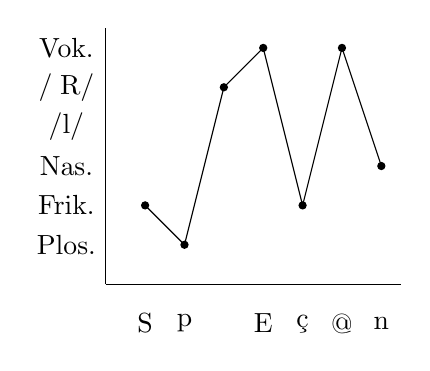
\begin{tikzpicture}[scale=0.5]
			\draw[black] (-1,0) -- (6.5,0) ; % x axis
			\draw[black] (-1,0) -- (-1,6.5); % y axis
			\node at (-2,1) {Plos.};
			\node at (-2,2) {Frik.};
			\node at (-2,3) {Nas.};
			\node at (-2,4) {\textipa{/l/}};
			\node at (-2,5) {\textipa{/\;R/}};
			\node at (-2,6) {Vok.};
			\draw[black] (0,2) -- (1,1) -- (2,5) -- (3,6) -- (4,2) -- (5,6) -- (6,3);
			\node at (0,-1) {\textipa{S}};
			\node at (1,-1) {\textipa{p}};
			\node at (2,-1) {\textipa{\textscr}};
			\node at (3,-1) {\textipa{E}};
			\node at (4,-1) {\textipa{\c{c}}};
			\node at (5,-1) {\textipa{@}};
			\node at (6,-1) {\textipa{n}};
			\fill (0,2) circle [radius=3pt];
			\fill (1,1) circle [radius=3pt];
			\fill (2,5) circle [radius=3pt];
			\fill (3,6) circle [radius=3pt];
			\fill (4,2) circle [radius=3pt];
			\fill (5,6) circle [radius=3pt];
			\fill (6,3) circle [radius=3pt];
			\end{tikzpicture}}
	\end{figure}
\end{minipage}
\begin{minipage}{.05\textwidth}
	\hfill
\end{minipage}
\begin{minipage}{.45\textwidth}
	\begin{figure}
		\centering
		\scalebox{.75}{
		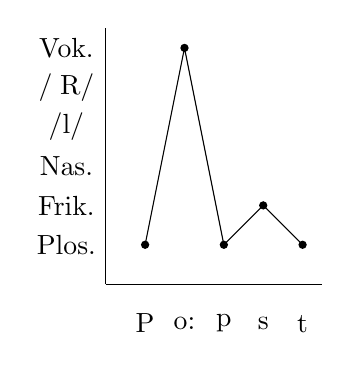
\begin{tikzpicture}[scale=0.5]
			\draw[black] (-1,0) -- (4.5,0) ; % x axis
			\draw[black] (-1,0) -- (-1,6.5); % y axis
			\node at (-2,1) {Plos.};
			\node at (-2,2) {Frik.};
			\node at (-2,3) {Nas.};
			\node at (-2,4) {\textipa{/l/}};
			\node at (-2,5) {\textipa{/\;R/}};
			\node at (-2,6) {Vok.};
			\draw[black] (0,1) -- (1,6) -- (2,1) -- (3,2) -- (4,1);
			\node at (0,-1) {\textipa{P}};
			\node at (1,-1) {\textipa{o:}};
			\node at (2,-1) {\textipa{p}};
			\node at (3,-1) {\textipa{s}};
			\node at (4,-1) {\textipa{t}};
			\fill (0,1) circle [radius=3pt];
			\fill (1,6) circle [radius=3pt];
			\fill (2,1) circle [radius=3pt];
			\fill (3,2) circle [radius=3pt];
			\fill (4,1) circle [radius=3pt];
			\end{tikzpicture}}
	\end{figure}
\end{minipage}

\end{frame}
%%%%%%%%%%%%%%%%%%%%%%%%%%%%%%%%%

\begin{frame}
\frametitle{Lösungen}
%
\begin{minipage}{.3\textwidth}
	\centering
	\scalebox{.75}{\begin{forest} MyP edges, [,phantom
[$\sigma$
	[O
		[x, tier=word[\textipa{b}]]
		[x, tier=word[\textipa{\textscr}]]
	]
	[R
		[N	[x, tier=word[\textipa{a}]]
		]
		[K
			[x[\textipa{n}]]
			[x[\textipa{t.}]]
		]
	]  
]
[$\sigma$
	[O	[x, tier=word[\textipa{S}]]
	]
	[R	
		[N	
			[x[\textipa{U}]]
		]
		[K	
			[x[\textipa{\t{ts}}]]
		]
	]
]]
	\end{forest}}
	
\end{minipage}
%
\begin{minipage}{.05\textwidth}
	\hfill
\end{minipage}
%
\begin{minipage}{.6\textwidth}
\centering
\scalebox{.75}{
\begin{forest}
	MyP edges, [, phantom
[$ \sigma $
	[O
		[x, tier=word[\textipa{P}]]
	]
	[R
		[N
			[x, tier=word[\textipa{a}]]
		]
		[K
			[x[\textipa{p}]]
		]
	]
]
[$ \sigma $
	[O
		[x, tier=word[\textipa{S}]]
		[x, tier=word[\textipa{t}]]
	]
	[R
		[N
			[x[\textipa{a}]]
		]
		[K
			[x[\textipa{n}]]
			[x[\textipa{\t{ts}}]]
		]
	]
]
[$ \sigma $
	[O
		[x, tier=word[\textipa{h}]]
	]
	[R
		[N
			[x[\textipa{a}]]
		]
		[K
			[x[\textipa{l}]]
		]
	]
]
[$ \sigma $
	[O
		[x, tier=word[t]]
	]
	[R	
		[N
			[x[\textipa{\textturna}]]
		]
	]
]]
\end{forest}}
\end{minipage}

\begin{minipage}{.3\textwidth}
	\begin{figure}
		\centering
		\scalebox{.75}{
			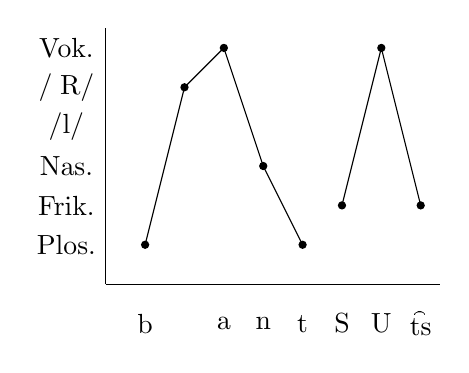
\begin{tikzpicture}[scale=0.5]
			\draw[black] (-1,0) -- (7.5,0) ; % x axis
			\draw[black] (-1,0) -- (-1,6.5); % y axis
			\node at (-2,1) {Plos.};
			\node at (-2,2) {Frik.};
			\node at (-2,3) {Nas.};
			\node at (-2,4) {\textipa{/l/}};
			\node at (-2,5) {\textipa{/\;R/}};
			\node at (-2,6) {Vok.};
			\draw[black] (0,1) -- (1,5) -- (2,6) -- (3,3) -- (4,1);
			\draw[black] (5,2) -- (6,6) -- (7,2);
			\node at (0,-1) {\textipa{b}};
			\node at (1,-1) {\textipa{\textscr}};
			\node at (2,-1) {\textipa{a}};
			\node at (3,-1) {\textipa{n}};
			\node at (4,-1) {\textipa{t}};
			\node at (5,-1) {\textipa{S}};
			\node at (6,-1) {\textipa{U}};
			\node at (7,-1) {\textipa{\t{ts}}};
			\fill (0,1) circle [radius=3pt];
			\fill (1,5) circle [radius=3pt];
			\fill (2,6) circle [radius=3pt];
			\fill (3,3) circle [radius=3pt];
			\fill (4,1) circle [radius=3pt];
			\fill (5,2) circle [radius=3pt];
			\fill (6,6) circle [radius=3pt];
			\fill (7,2) circle [radius=3pt];
			\end{tikzpicture}}
	\end{figure}
\end{minipage}
\begin{minipage}{.05\textwidth}
	\hfill
\end{minipage}
\begin{minipage}{.6\textwidth}
\begin{figure}
			\centering
			\scalebox{.75}{
			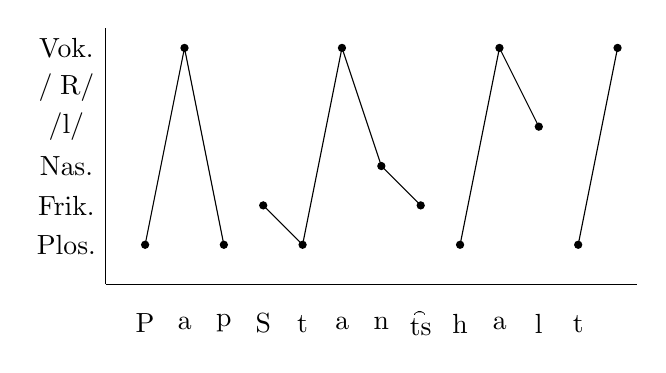
\begin{tikzpicture}[scale=0.5]
			\draw[black] (-1,0) -- (12.5,0) ; % x axis
			\draw[black] (-1,0) -- (-1,6.5); % y axis
			\node at (-2,1) {Plos.};
			\node at (-2,2) {Frik.};
			\node at (-2,3) {Nas.};
			\node at (-2,4) {\textipa{/l/}};
			\node at (-2,5) {\textipa{/\;R/}};
			\node at (-2,6) {Vok.};
			\draw[black] (0,1)--(1,6)--(2,1);
			\draw[black](3,2)--(4,1)--(5,6)--(6,3)--(7,2);
			\draw[black](8,1)--(9,6)--(10,4);
			\draw[black](11,1)--(12,6);
			\fill (0,1) circle [radius=3pt];
			\fill (1,6) circle [radius=3pt];
			\fill (2,1) circle [radius=3pt];
			\fill (3,2) circle [radius=3pt];
			\fill (4,1) circle [radius=3pt];
			\fill (5,6) circle [radius=3pt];
			\fill (6,3) circle [radius=3pt];
			\fill (7,2) circle [radius=3pt];
			\fill (8,1) circle [radius=3pt];
			\fill (9,6) circle [radius=3pt];
			\fill (10,4) circle [radius=3pt];
			\fill (11,1) circle [radius=3pt];
			\fill (12,6) circle [radius=3pt];
			\node at (0,-1){\textipa{P}};
			\node at (1,-1){\textipa{a}};
			\node at (2,-1){\textipa{p}};
			\node at (3,-1){\textipa{S}};
			\node at (4,-1){\textipa{t}};
			\node at (5,-1){\textipa{a}};
			\node at (6,-1){\textipa{n}};
			\node at (7,-1){\textipa{\t{ts}}};
			\node at (8,-1){\textipa{h}};
			\node at (9,-1){\textipa{a}};
			\node at (10,-1){\textipa{l}};
			\node at (11,-1){\textipa{t}};
			\node at (12,-1){\textipa{\textturna}};
			\end{tikzpicture}}
	\end{figure}
\end{minipage}


\end{frame}

}

%%%%%%%%%%%%%%%%%%%%%%%%%%%%%%%%%%%%%%%%%%%%%%%%%%%%%%%%%%%%%%

\subsection{Silbengelenk}
\iftoggle{toc}{
\frame{
\frametitle{~}
\begin{multicols}{2}
	\tableofcontents[currentsection]
\end{multicols}	
}
}
%%%%%%%%%%%%%%%%%%%%%%%%%%%%%%%%%%

\begin{frame}
\frametitle{Silbengelenk}


\begin{minipage}{.63\textwidth}

\begin{itemize}
	\item \textbf{ambisyllabischer Konsonant}
	
	\item[]
	\item Ein Konsonant,\\
               der zugleich \textbf{zu zwei Silben} gehört. 
	
	\item[]
	\item Nur \textbf{eine X Position} (nur eine Zeiteinheit, vgl. echte Geminaten)
	
\end{itemize}
\end{minipage}
%
\begin{minipage}{.35\textwidth}
%%%%%%%%%%%%%%
%%% Forestset Syllables

\newbox\foreststrutbox
\setbox\foreststrutbox=\hbox to 0pt{\phantom{\forestOve{standard node}{content}}}
\def\foreststrut{\copy\foreststrutbox}
\forestset{
GP1/.style 2 args={
for n={1}{baseline},
s sep=0pt, l sep=0pt,
for descendants={
l sep=0pt, l={#1},
anchor=base,calign=first,child anchor=north,
inner xsep=1pt,inner ysep=2pt,outer sep=0pt,s sep=0pt,
},
delay={
if content={}{phantom}{for children={no edge}},
for tree={
if content={O}{tier=OR}{},
if content={R}{tier=OR}{},
if content={N}{tier=N}{},
if content={x}{
tier=x,content={$\times$},outer xsep={#2},
for tree={calign=center},
for descendants={content format={\foreststrut\forestoption{content}}},
before drawing tree={outer xsep=0pt,delay={typeset node}},
s sep=4pt
}{},
},
},
before drawing tree={where content={}{parent anchor=center,child anchor=center}{}},
},
GP1/.default={5ex}{8.0pt},
associate/.style={%
tikz+={\draw(!)--(!#1);}},
spread/.style={
before drawing tree={tikz+={\draw[dotted](!)--(!#1);}}},
govern/.style={
before drawing tree={tikz+={\draw[->](!)--(!#1);}}},
p-govern/.style={
before drawing tree={tikz+={\draw[->](.north) to[out=150,in=30] (!#1.north);}}},
no p-govern/.style={
before drawing tree={tikz+={\draw[->,loosely dashed](.north) to[out=150,in=30] (!#1.north);}}},
encircle/.style={before drawing tree={circle,draw,inner sep=0pt}},
fen/.style={pin={[font=\footnotesize,inner sep=1pt,pin edge=<-]10:\textsc{Fen}}},
el/.style={content=\textsc{\textbf{##1}}},
head/.style={content=\textsc{\textbf{\underline{##1}}}},
llap/.style={
tikz+={%
\edef\forest@temp{\noexpand\node[\option{node options},
anchor=base east,at=(.base east)]}%
\forest@temp{#1\phantom{\option{environment}}};
}
},
rlap/.style={
tikz+={%
\edef\forest@temp{\noexpand\node[\option{node options},
anchor=base west,at=(.base west)]}%
\forest@temp{\phantom{\option{environment}}#1};
}
},
}
%%%%%%%%%%%%%

\footnotesize
\centering
\begin{forest} MyP edges, [,phantom
  [$\sigma$
    [O
    	[x, tier=word
    		[\textipa{t}]
    	]
    ]
    [R
    	[N
    		[x, tier=word
    			[\textipa{I}]
    		]
    	]  		
    	[K 
    		[x, name=x
    			[\textipa{k}]
    		]
    	]
    ]
  ]
  [$\sigma$
    [O, name=onset 
    ]
    [R
    	[N
    		[x
    			[\textipa{@}]
    		]
    	]
    	[K [x[\textipa{n}]]]]
  ]  
]
{
\draw[black] (x.north)--(onset.south);
}
\end{forest}

\end{minipage}

\end{frame}



%%%%%%%%%%%%%%%%%%%%%%%%%%%%%%%%%%

\begin{frame}
%\frametitle{Silbengelenk}

\begin{minipage}{.35\textwidth}
%%%%%%%%%%%%%%
%%% Forestset Syllables

\newbox\foreststrutbox
\setbox\foreststrutbox=\hbox to 0pt{\phantom{\forestOve{standard node}{content}}}
\def\foreststrut{\copy\foreststrutbox}
\forestset{
GP1/.style 2 args={
for n={1}{baseline},
s sep=0pt, l sep=0pt,
for descendants={
l sep=0pt, l={#1},
anchor=base,calign=first,child anchor=north,
inner xsep=1pt,inner ysep=2pt,outer sep=0pt,s sep=0pt,
},
delay={
if content={}{phantom}{for children={no edge}},
for tree={
if content={O}{tier=OR}{},
if content={R}{tier=OR}{},
if content={N}{tier=N}{},
if content={x}{
tier=x,content={$\times$},outer xsep={#2},
for tree={calign=center},
for descendants={content format={\foreststrut\forestoption{content}}},
before drawing tree={outer xsep=0pt,delay={typeset node}},
s sep=4pt
}{},
},
},
before drawing tree={where content={}{parent anchor=center,child anchor=center}{}},
},
GP1/.default={5ex}{8.0pt},
associate/.style={%
tikz+={\draw(!)--(!#1);}},
spread/.style={
before drawing tree={tikz+={\draw[dotted](!)--(!#1);}}},
govern/.style={
before drawing tree={tikz+={\draw[->](!)--(!#1);}}},
p-govern/.style={
before drawing tree={tikz+={\draw[->](.north) to[out=150,in=30] (!#1.north);}}},
no p-govern/.style={
before drawing tree={tikz+={\draw[->,loosely dashed](.north) to[out=150,in=30] (!#1.north);}}},
encircle/.style={before drawing tree={circle,draw,inner sep=0pt}},
fen/.style={pin={[font=\footnotesize,inner sep=1pt,pin edge=<-]10:\textsc{Fen}}},
el/.style={content=\textsc{\textbf{##1}}},
head/.style={content=\textsc{\textbf{\underline{##1}}}},
llap/.style={
tikz+={%
\edef\forest@temp{\noexpand\node[\option{node options},
anchor=base east,at=(.base east)]}%
\forest@temp{#1\phantom{\option{environment}}};
}
},
rlap/.style={
tikz+={%
\edef\forest@temp{\noexpand\node[\option{node options},
anchor=base west,at=(.base west)]}%
\forest@temp{\phantom{\option{environment}}#1};
}
},
}
%%%%%%%%%%%%%

\footnotesize
\centering
\begin{forest} MyP edges, [, phantom
  [$\sigma$
    [O
    	[x, tier=word
    		[\textipa{k}]
    	]
    	[x, tier=word	[\textipa{l}]]
    ]
    [R
    	[N
    		[x, tier=word
    			[\textipa{I}]
    		]
    	]  		
    	[K 
    		[x, name=x
    			[\textipa{N}]
    		]
    	]
    ]
  ]
  [$\sigma$
    [O, name=onset
    ]
    [R
    	[N
    		[x
    			[\textipa{@}]
    		]
    	]
    	[K [x[\textipa{n}]]]]
  ]  
]
{
\draw[black] (x.north)--(onset.south);
}
\end{forest}

\end{minipage}
%
\begin{minipage}{.63\textwidth}

\begin{itemize}
	\item \textbf{In der Schreibung} werden Silbengelenke häufig mit Doppelkonsonanten markiert (aber nicht immer!)
	
	\ea der \textipa{[\t{tS}Et]} \vs ich \textipa{[\t{tS}Et@]}\\
	\pause der Cha\alertred{t} \vs ich cha\alertred{tt}e
	\z
	\ea
        abkli\alertred{ng}en, zwi\alertred{sch}en
        \z
% abklingngen, zwischschen durch ästhetisches Prinzip verboten

\pause
	
	\item \textbf{Silbengelenke kommen nach betonten ungespannten Vokalen vor. }
	
	Ungespannte betonte Vokale kommen nicht in offenen Silben vor.

	\item Linear: \textbf{Markierung} durch Punkt
	
	  \ea
          \textipa{[Pap.klI\.N@n]}
          \z
	
\end{itemize}

\end{minipage}

\end{frame}



%%%%%%%%%%%%%%%%%%%%%%%%%%%%%%%%%%
%%%%%%%%%%%%%%%%%%%%%%%%%%%%%%%%%%
\subsection{Silbifizierung}
\iftoggle{toc}{
\frame{
\frametitle{~}
\begin{multicols}{2}
	\tableofcontents[currentsection]
\end{multicols}	
}
}
%%%%%%%%%%%%%%%%%%%%%%%%%%%%%%%%%%

\begin{frame}
\frametitle{Silbifizierung}

\begin{itemize}
	\item Silbifizierung, Syllabierung $:=$ in Silben einteilen
	\item[]
	\item Wie würden Sie folgende Lautsequenzen silbifizieren?:

	  \ea
          ata, odo, eke
          \z

\pause

	\item Ein einziger intervokalischer Konsonant wird immer als Silbenanlaut silbifiziert (universelles Prinzip: \textbf{Onset-Maximierung})
	
	
\end{itemize}

\begin{block}{Onsetmaximierung}
Bilde zuerst den größtmöglichen Silbenanlaut;\\ dann bilde den Silbenauslaut \citep[218]{Hall00a}
\end{block}

\end{frame}



%%%%%%%%%%%%%%%%%%%%%%%%%%%%%%%%%%

\begin{frame}
%\frametitle{Silbifizierung}

\begin{block}{Onsetmaximierung}
Bilde zuerst den größtmöglichen Silbenanlaut; dann bilde den Silbenauslaut \citep[218]{Hall00a}
\end{block}


\begin{itemize}
	\item Onset-Maximierung herleitbar aus:
	\begin{enumerate}
		\item Silbenanlautgesetz (CV häufiger als V), und
		\item Silbenauslautgesetz (CVC$^{n} >$ CVC$^{n+1}$)
	\end{enumerate}

\pause
	\item Silbifizierung nicht über Morphemgrenzen hinweg! 
	\item Ausnahme: Suffixe mit vokalischem Onset:
	
	  \ea
          kind\#isch: \textipa{[kIn.dIS]}
          \z
	
	  \ea
          kind\#lich: \textipa{[kInt.lI\c{c}]}
          \z
          
     \item \# := Morphemgrenze

% Wenn man Morphmgrenzenbedingung weglassen würde, ergäbe sich Bra. ndschutz

% rek.nen vs. re.gnen
	
\end{itemize}

\end{frame}


%%%%%%%%%%%%%%%%%%%%%%%%%%%%%%%%%%
%%%%%%%%%%%%%%%%%%%%%%%%%%%%%%%%%%
%\subsection{Übung}
%\iftoggle{toc}{
%\frame{
%\frametitle{~}
%\begin{multicols}{2}
%	\tableofcontents[currentsection]
%\end{multicols}	
%}
%}
%%%%%%%%%%%%%%%%%%%%%%%%%%%%%%%%%%

\begin{frame}
\frametitle{Übung}

\begin{itemize}
	\item Was bedeutet die Annahme des Sonoritätsprinzips und der Onset-Maximierung für die folgenden Beispielwörter:
	
	  \ea
          Fabrik, Imker, neblig, Falter, regnen
          \z
\end{itemize}	
\pause

\iftoggle{loesung}{
	\begin{itemize}
		\item[] \textcolor{red}{\textipa{[fa:.b\textscr Ik]}, \textipa{[PIm.k5]}, \textipa{[ne:.blI\c{c}]}, \textipa{[fal.t5]}, \textipa{[\textscr e:.gn@n]}}
	\item [] \textcolor{red}{Koda: *Obstruent vor Sonorant} 
	\item [] \textcolor{red}{Onset: *Sonorant vor Obstruent}
	\end{itemize}
}

\begin{itemize}
	\item Welche Prinzipien bzw. Regularitäten werden verletzt bei:
\end{itemize}

\begin{minipage}{.4\textwidth}
	\eal
	\ex \textipa{[PE.b@]}
	\ex \textipa{[PEb.@]}
	\ex \textipa{[PEp.@]}
	\ex \textipa{[PEp.b@]}
        \zl
\end{minipage}
\begin{minipage}{.4\textwidth}
	\pause	
	\begin{itemize}
	\item[] \textcolor{red}{\ras Kurzvokal}
	\item[] \textcolor{red}{\ras Auslautverhärtung}
	\item[] \textcolor{red}{\ras Onset-Maximierung}
	\item[] \textcolor{red}{\ras keine Regelverletzung}
	\end{itemize}
	
\end{minipage}

\end{frame}



%%%%%%%%%%%%%%%%%%%%%%%%%%%%%%%%%%



\begin{frame}
\frametitle{Übung}

\begin{itemize}
	\item Silbifizieren Sie folgende Segmentsequenzen in zwei Schritten
	\begin{itemize}
		\item Onsetmaximierungsprinzip
		\item Sonoritätsprinzip
	\end{itemize}

\item Stellen Sie fest, ob alle Silben wohlgeformt sind.\\
      Falls nicht, benennen Sie die Verletzungen
	
\ea\label{ex:Otling}
\textipa{[o:tlIN5mSplag\textscr e:hOn]}
\z

% Otlingamsplagrehon
	\ea\label{ex:Blumentopf}
	Blumentopferde
	\z

\end{itemize}

% blu.men.to.pfer.de

%\ea
%Urinstinkt
%\z	

\end{frame}


%%%%%%%%%%%%%%%%%%%%%%%%%%%%%%%%%%%%%%%
\begin{frame}
\frametitle{Lösung}

zu (\ref{ex:Otling}):

\textcolor{red}{zuerst Onset"=Maximierung: \textipa{o:.tlI.\ng \textturna. mSpla .g\textscr e: .hOn}}\\
\textcolor{red}{dann Anwendung des Sonoritätsprinzips: \textipa{o:.tlI\ng \textturna mS .pla .g\textscr e: .hOn}}

zu (\ref{ex:Blumentopf}): 

\textcolor{red}{zuerst Onset-Maximierung: \textipa{blu: .m@ .nto: .pfE .{\textscr}d@}}\\
\textcolor{red}{dann Awendung des Sonoritätsprinzip: \textipa{blu: .m@n .to: .pfE{\textscr} .d@}}






\end{frame}
	


% ' Stahl , tische     Hauptbetonung auf Stahl, Nebenbetonung auf Tische


%%%%%%%%%%%%%%%%%%%%%%%%%%%%%%%%%%
%%%%%%%%%%%%%%%%%%%%%%%%%%%%%%%%%%
\subsection{Exkurs: Akzent}
\iftoggle{toc}{
\frame{
\frametitle{~}
\begin{multicols}{2}
	\tableofcontents[currentsection]
\end{multicols}	
}
}
%%%%%%%%%%%%%%%%%%%%%%%%%%%%%%%%%%

\begin{frame}
\frametitle{Exkurs: Akzent}

\begin{itemize}
	\item Silben können \textbf{betont} oder \textbf{unbetont} sein, d.\,h. sie können einen Akzent tragen oder nicht
	\item[]

\begin{block}{Akzent}
\textbf{Auditiver Eindruck der Prominenz eines Vokals} gegenüber einem anderen durch (relational, nicht absolut!):
\begin{itemize}
	\item Lautstärke
	\item Dauer
	\item Höhere Tonlage
	\item Ausgeprägtere Artikulationsbewegungen
\end{itemize}
\end{block}	 
	
	\item[]
	\item Man unterscheidet zwischen \textbf{Wort-} und \textbf{Satzakzent} (engl. \emph{stress} und \emph{accent})

\end{itemize}

\end{frame}



%%%%%%%%%%%%%%%%%%%%%%%%%%%%%%%%%%%
%%%%%%%%%%%%%%%%%%%%%%%%%%%%%%%%%%
%\subsubsection{Exkurs: Wortakzent}
%\frame{
%\begin{multicols}{2}
%\frametitle{~}
%	\tableofcontents[currentsection]
%\end{multicols}
%}
%%%%%%%%%%%%%%%%%%%%%%%%%%%%%%%%%%

\begin{frame}
\frametitle{Exkurs: Wortakzent}

\begin{itemize}
	\item Was scheint die häufigste Betonung im Deutschen zu sein?
	
	  \ea
          Mutter, Männer, Autos, Hühner, Lehrer, Kinder, alle \ldots
          \z
	
\pause
	\textbf{betont-unbetont (Trochäus)}
	
	\item Ausnahmen (die je nach Theorie verschieden erklärt werden):

\end{itemize}

\begin{minipage}{.4\textwidth}
		
	\eal 
	\ex \textipa{['f\textscr aU]}
	\ex \textipa{[mu.'zi:k]}
	\ex \textipa{[le:.b@n.d@]}
	\ex \textipa{[pa.pa.'g\t{aɪ}]}
	\ex \textipa{[f\t{ɛɐ}.'Pa5.b\t{aɪ}.t@n]}
	\zl

\end{minipage}
\begin{minipage}{.5\textwidth}
	
	\iftoggle{loesung}{
	\begin{itemize}
		\item[] \textcolor{red}{\ras nur eine Silbe }
		\item[] \textcolor{red}{\ras Fremdwort}
		\item [] \textcolor{red}{\ras Flektierte Elemente \ab{-de}}
		\item [] \textcolor{red}{\ras Fremdwort}
		\item [] \textcolor{red}{\ras Derivation \ab{ver-}}
	\end{itemize}
}

\end{minipage}

\end{frame}



%%%%%%%%%%%%%%%%%%%%%%%%%%%%%%%%%%%
%%%%%%%%%%%%%%%%%%%%%%%%%%%%%%%%%%
%\subsubsection{Exkurs: Satzakzent}
%\frame{
%\begin{multicols}{2}
%\frametitle{~}
%	\tableofcontents[currentsection]
%\end{multicols}
%}
%%%%%%%%%%%%%%%%%%%%%%%%%%%%%%%%%%

\begin{frame}
\frametitle{Exkurs: Satzakzent}

\begin{itemize}
	\item In einem Satz können betonte Silben \textbf{noch weiter hervorgehoben} werden (dabei meist durch die Tonhöhe):
	
	\eal 
	\ex Géstern hat BAyern gewónnen.
	\ex GÉStern hat Báyern gewónnen.
	\ex Géstern hat Báyern geWONnen.
	\zl
	\item Die prominenteste Silbe im Satz wird meist mit \textbf{Großbuchstaben} dargestellt, sie trägt den Satzakzent

	\item Durch diese Akzentuierung wird das gesamte Wort
hervorgehoben \ras \textbf{Fokus des Satzes} (\gqq{Informationsstruktur})
	
\end{itemize}

\end{frame}



%%%%%%%%%%%%%%%%%%%%%%%%%%%%%%%%%%%
%%%%%%%%%%%%%%%%%%%%%%%%%%%%%%%%%%
%\subsubsection{Exkurs: Intonation}
%\frame{
%\begin{multicols}{2}
%\frametitle{~}
%	\tableofcontents[currentsection]
%\end{multicols}
%}
%%%%%%%%%%%%%%%%%%%%%%%%%%%%%%%%%%

\begin{frame}
\frametitle{Exkurs: Intonation}

\begin{block}{Intonation}
Tonhöhenverlauf (\gqq{Melodie}) einer Äußerung
\end{block}

\begin{itemize}
	\item \textbf{Satztypen} können mittels Intonation unterschieden werden.
	
	\item Sprechen Sie die folgenden Äußerungen mit fallender und steigender Intonation
	\eal 
	\ex Heute gewinnen die Bayern.
	\ex Schon Schluss.
        \zl
\pause
	\textbf{Aussage-} \vs \textbf{Interrogativsatz}	
	
\end{itemize}

\end{frame}



%%%%%%%%%%%%%%%%%%%%%%%%%%%%%%%%%%

\begin{frame}
%\frametitle{Exkurs: Intonation}

\begin{itemize}
	\item Ambige ($\approx$ mehrdeutige) Sätze können mittels Intonation \gs{durch die sog. Hutkontur} \textbf{disambiguiert} werden: 
	
	  \ea
          Alle Studenten haben die Klausur nicht bestanden.
          \z
        \eal
	\ex Es ist nicht der Fall, dass alle Studenten die Klausur bestanden haben. \hfill $\lsem \neg \forall \rsem$
	\ex Für alle Studenten gilt, dass sie die Klausur nicht bestanden haben. \hfill $\lsem \forall \neg \rsem$
        \zl
\pause 

\ea
/Alle Studenten haben die Klausur  nicht\textbackslash\ bestanden.
\z
\eal
\ex Es ist nicht der Fall, dass alle Studenten die Klausur bestanden haben. \hfill $\lsem \neg \forall \rsem$
	\zl

\end{itemize}

\end{frame}


\iftoggle{hausaufgabe}{
	
	\subsection{Hausaufgabe}
	\iftoggle{toc}{
		\frame{
			\frametitle{~}
			\begin{multicols}{2}
				\tableofcontents[currentsection]
			\end{multicols}	
		}
	}
	
	
%%%%%%%%%%%%%%%%%%%%%%%%%%%%%%%%%%
\begin{frame}%[allowframebreaks]
	\frametitle{Hausaufgabe}
\begin{itemize}
			
	\item[1.] Geben Sie eine phonetische Tranksription der folgenden Wörter nach der \gqq{Standardaussprache} an, zeichnen Sie dabei die Silbestruktur nach dem Konstituentenmodell und mit der Skelettschicht, und geben Sie die Sonoritätsprofile an.
		
		\eal \label{ex:HA1}
		\ex Stimmenfang \label{ex:HA1a}
		\ex Mittagessen\label{ex:HA1b}
		\ex Bierdeckel\label{ex:HA1c}
		\zl
\end{itemize}

\begin{block}{Sonoritätshierarchie (Zur Erinnerung)}
	Vokal $>$ \textipa{/\textscr /} $>$ \textipa{/l/} $>$ Nasal $>$ Frikativ $>$ Plosiv \\
	$x > y :=$ $x$ ist sonorer als $y$
\end{block}

\end{frame}

%%%%%%%%%%%%%%%%%%%%%%%%%%%%%%%%%%%%%%%%%%%%%%%%%%%%%

\begin{frame}
\begin{itemize}
	\item[2.] Silbifizieren Sie folgende Segmentsequenzen in zwei Schritten
	\begin{itemize}
		\item Onsetmaximierungsprinzip
		\item Sonoritätsprinzip
	\end{itemize}
	
	Stellen Sie fest, ob alle Silben wohlgeformt sind. Falls nicht, benennen Sie die Verletzungen	
	\ea\label{ex:HA2}
	Urinstinkt
	\z	
	\item[3.] Geben Sie die standarddeutsche phonetische Transkription des Wortes \ab{Stahltische} inklusive der Silbenstruktur (mit X-Skelettschicht) an. Ermitteln Sie die Kriterien, die bei der Silbifizierung wirken.
	
	\item[4.] Geben Sie die Gründe an, warum die folgenden Wörter aus phonetisch/ phonologischen Gründen im Deutschen nicht möglich sind:
	
	\eal\label{ex:HA3}
	\ex[*]{\textipa{['Napl.O:t]}}
	\ex[*]{\textipa{[a\;R.'tUng]}}
	\zl
	
\end{itemize}

\end{frame}
	
}


%%%%%%%%%%%%%%%%%%%%%%%%%%%% Lösungen %%%%%%%%%%%%%%%%%%%%%%%%%%%%%%

\iftoggle{loesung}{
	
	\subsection{Lösung}
	\iftoggle{toc}{
		\frame{
			\frametitle{~}
			\begin{multicols}{2}
				\tableofcontents[currentsection]
			\end{multicols}	
		}
	}
	
	
%%%%%%%%%%%%%%%%%%%%%%%%%%%%%%%%%%
\begin{frame}%[allowframebreaks]
	\frametitle{Lösung}
	\begin{itemize}
			
		\item[1.] Geben Sie eine phonetische Tranksription der folgenden Wörter nach der \gqq{Standardaussprache} an, zeichnen Sie dabei die Silbestruktur nach dem Konstituentenmodell und mit der Skelettschicht, und geben Sie die Sonoritätsprofile an.
			
			\begin{exe}
				\exi{(\ref{ex:HA1})}
				\begin{xlist}
					\ex Stimmenfang
					\ex Mittagessen
					\ex Bierdeckel
				\end{xlist}
			\end{exe}

			\begin{block}{Sonoritätshierarchie (Zur Erinnerung)}
		Vokal $>$ \textipa{/\textscr /} $>$ \textipa{/l/} $>$ Nasal $>$ Frikativ $>$ Plosiv \\
		$x > y :=$ $x$ ist sonorer als $y$
	\end{block}
			
	\end{itemize}
\end{frame}

\begin{frame}

%\begin{minipage}{.35\textwidth}
			%%%%%%%%%%%%%%
%%% Forestset Syllables

\newbox\foreststrutbox
\setbox\foreststrutbox=\hbox to 0pt{\phantom{\forestOve{standard node}{content}}}
\def\foreststrut{\copy\foreststrutbox}
\forestset{
GP1/.style 2 args={
for n={1}{baseline},
s sep=0pt, l sep=0pt,
for descendants={
l sep=0pt, l={#1},
anchor=base,calign=first,child anchor=north,
inner xsep=1pt,inner ysep=2pt,outer sep=0pt,s sep=0pt,
},
delay={
if content={}{phantom}{for children={no edge}},
for tree={
if content={O}{tier=OR}{},
if content={R}{tier=OR}{},
if content={N}{tier=N}{},
if content={x}{
tier=x,content={$\times$},outer xsep={#2},
for tree={calign=center},
for descendants={content format={\foreststrut\forestoption{content}}},
before drawing tree={outer xsep=0pt,delay={typeset node}},
s sep=4pt
}{},
},
},
before drawing tree={where content={}{parent anchor=center,child anchor=center}{}},
},
GP1/.default={5ex}{8.0pt},
associate/.style={%
tikz+={\draw(!)--(!#1);}},
spread/.style={
before drawing tree={tikz+={\draw[dotted](!)--(!#1);}}},
govern/.style={
before drawing tree={tikz+={\draw[->](!)--(!#1);}}},
p-govern/.style={
before drawing tree={tikz+={\draw[->](.north) to[out=150,in=30] (!#1.north);}}},
no p-govern/.style={
before drawing tree={tikz+={\draw[->,loosely dashed](.north) to[out=150,in=30] (!#1.north);}}},
encircle/.style={before drawing tree={circle,draw,inner sep=0pt}},
fen/.style={pin={[font=\footnotesize,inner sep=1pt,pin edge=<-]10:\textsc{Fen}}},
el/.style={content=\textsc{\textbf{##1}}},
head/.style={content=\textsc{\textbf{\underline{##1}}}},
llap/.style={
tikz+={%
\edef\forest@temp{\noexpand\node[\option{node options},
anchor=base east,at=(.base east)]}%
\forest@temp{#1\phantom{\option{environment}}};
}
},
rlap/.style={
tikz+={%
\edef\forest@temp{\noexpand\node[\option{node options},
anchor=base west,at=(.base west)]}%
\forest@temp{\phantom{\option{environment}}#1};
}
},
}
%%%%%%%%%%%%%

\begin{minipage}{.2\textwidth}
	\centering
Zu (\ref{ex:HA1a}):
\end{minipage}
%
\begin{minipage}{.7\textwidth}
	\begin{figure}
\footnotesize
\centering
			\begin{forest} MyP edges, [, phantom
				[$\sigma$
				[O [x, tier=word [\textipa{S}]] [x, tier=word [\textipa{t}]]]
				[R [N [x, tier=word [\textipa{I}]]] [K [x, name=x [\textipa{m}]]]]
				]
				[$\sigma$
				[O, name=onset]
				[R [N [x [\textipa{@}]]] [K [x [\textipa{n}]]]]
				]
				[$\sigma$
				[O [x, tier=word [\textipa{f}]]]
				[R [N [x [\textipa{a}]]] [K [x [\textipa{N}]]]]
				]
				]				
				{
					\draw[black] (x.north)--(onset.south);
				}
			\end{forest}
		
		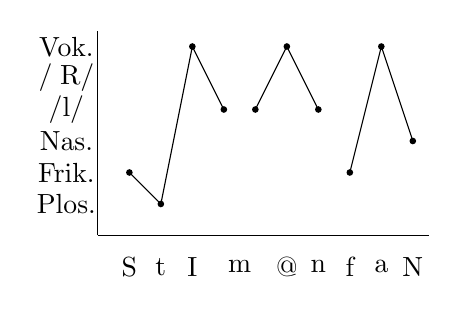
\begin{tikzpicture}[scale=0.4]
		\draw[black] (-1,0) -- (9.5,0) ; % x axis
		\draw[black] (-1,0) -- (-1,6.5); % y axis
		\node at (-2,1) {Plos.};
		\node at (-2,2) {Frik.};
		\node at (-2,3) {Nas.};
		\node at (-2,4) {\textipa{/l/}};
		\node at (-2,5) {\textipa{/\;R/}};
		\node at (-2,6) {Vok.};
		\draw[black] (0,2) -- (1,1) -- (2,6) -- (3,4);
		\draw[black] (4,4) -- (5,6) -- (6,4);
		\draw[black] (7,2) -- (8,6) -- (9,3);
		\node at (0,-1) {\textipa{S}};
		\node at (1,-1) {\textipa{t}};
		\node at (2,-1) {\textipa{I}};
		\node at (3.5,-1) {\textipa{m}};
		\node at (5,-1) {\textipa{@}};
		\node at (6,-1) {\textipa{n}};
		\node at (7,-1) {\textipa{f}};
		\node at (8,-1) {\textipa{a}};
		\node at (9,-1) {\textipa{N}};
		\fill (0,2) circle [radius=3pt];
		\fill (1,1) circle [radius=3pt];
		\fill (2,6) circle [radius=3pt];
		\fill (3,4) circle [radius=3pt];
		\fill (4,4) circle [radius=3pt];
		\fill (5,6) circle [radius=3pt];
		\fill (6,4) circle [radius=3pt];
		\fill (7,2) circle [radius=3pt];
		\fill (8,6) circle [radius=3pt];
		\fill (9,3) circle [radius=3pt];
		\end{tikzpicture}
\end{figure}

\end{minipage}
\end{frame}

%%%%%%%%%%%%%%%%%%%%%%%%%%%%%%%%%%%%%%%%%%%%%%%

\begin{frame}		

\begin{minipage}{.2\textwidth}
	\centering
	Zu (\ref{ex:HA1b}):
\end{minipage}	
%\end{minipage}%
\begin{minipage}{.7\textwidth}
\begin{figure}
	\footnotesize
	\centering
	\begin{forest} MyP edges, [, phantom
	[$\sigma$
	[O [x, tier=word [\textipa{m}]]] 
	[R [N [x, tier=word [\textipa{I}]]] [K [x, name=x1 [\textipa{t}]]]]
	]
	[$\sigma$
	[O, name=onset1]
	[R [N [x [\textipa{a}]]] [K [x [\textipa{k}]]]]
	]
	[$\sigma$
	[O [x, tier=word [\textipa{P}]]]
	[R [N [x [\textipa{E}]]] [K [x, name=x2 [\textipa{s}]]]]
	]
	[$\sigma$
	[O, name=onset2]
	[R [N [x [\textipa{@}]]] [K [x [\textipa{n}]]]]
	]
	]
	{
		\draw[black] (x1.north)--(onset1.south);
		\draw[black] (x2.north)--(onset2.south);
	}
	\end{forest}

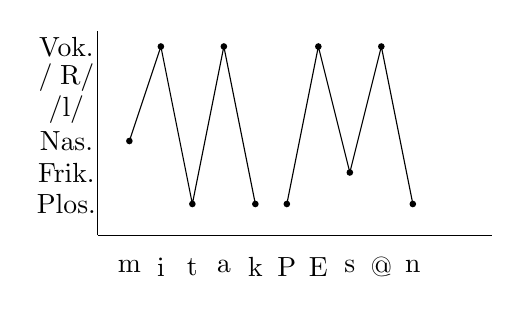
\begin{tikzpicture}[scale=0.4]
\draw[black] (-1,0) -- (11.5,0) ; % x axis
\draw[black] (-1,0) -- (-1,6.5); % y axis
\node at (-2,1) {Plos.};
\node at (-2,2) {Frik.};
\node at (-2,3) {Nas.};
\node at (-2,4) {\textipa{/l/}};
\node at (-2,5) {\textipa{/\;R/}};
\node at (-2,6) {Vok.};
\draw[black] (0,3) -- (1,6) -- (2,1) -- (3,6) -- (4,1);
\draw[black] (5,1) -- (6,6) -- (7,2) -- (8,6) -- (9,1);
\node at (0,-1) {\textipa{m}};
\node at (1,-1) {\textipa{i}};
\node at (2,-1) {\textipa{t}};
\node at (3,-1) {\textipa{a}};
\node at (4,-1) {\textipa{k}};
\node at (5,-1) {\textipa{P}};
\node at (6,-1) {\textipa{E}};
\node at (7,-1) {\textipa{s}};
\node at (8,-1) {\textipa{@}};
\node at (9,-1) {\textipa{n}};
\fill (0,3) circle [radius=3pt];
\fill (1,6) circle [radius=3pt];
\fill (2,1) circle [radius=3pt];
\fill (3,6) circle [radius=3pt];
\fill (4,1) circle [radius=3pt];
\fill (5,1) circle [radius=3pt];
\fill (6,6) circle [radius=3pt];
\fill (7,2) circle [radius=3pt];
\fill (8,6) circle [radius=3pt];
\fill (9,1) circle [radius=3pt];
\end{tikzpicture}
\end{figure}
\end{minipage}
	
\end{frame}

%%%%%%%%%%%%%%%%%%%%%%%%%%%%%%%%%%%%%%%%%%%%%%%

\begin{frame}

\begin{minipage}{.2\textwidth}
	\centering
	Zu (\ref{ex:HA1c}):
\end{minipage}	
\begin{minipage}{.7\textwidth}

	\begin{figure}
	\footnotesize
	\centering
	\begin{forest} MyP edges, [, phantom
	[$\sigma$
	[O [x,tier=word [\textipa{b}]]]
	[R [N [x, tier=word [\textipa{i:}, name=i]] [x,name=x1]] [K [x [\textipa{5}]]]]
	]
	[$\sigma$
	[O [x, tier=word [\textipa{d}]]]
	[R [N [x [\textipa{E}]]] [K [x, name=x [\textipa{k}]]]]
	]
	[$\sigma$
	[O, name=onset]
	[R [N [x, tier=word [\textipa{@}]]] [K [x [\textipa{l}]]]]
	]
	]
	{
		\draw[black] (x1.south)--(i.north);
		\draw[black] (x.north)--(onset.south);
	}
\end{forest}

\scalebox{.85}{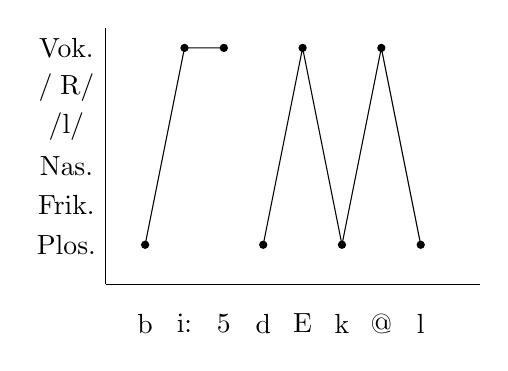
\begin{tikzpicture}[scale=0.5]
	\draw[black] (-1,0) -- (8.5,0) ; % x axis
	\draw[black] (-1,0) -- (-1,6.5); % y axis
	\node at (-2,1) {Plos.};
	\node at (-2,2) {Frik.};
	\node at (-2,3) {Nas.};
	\node at (-2,4) {\textipa{/l/}};
	\node at (-2,5) {\textipa{/\;R/}};
	\node at (-2,6) {Vok.};
	\draw[black] (0,1) -- (1,6) -- (2,6);
	\draw[black] (3,1) -- (4,6) -- (5,1) -- (6,6) -- (7,1);
	\node at (0,-1) {\textipa{b}};
	\node at (1,-1) {\textipa{i:}};
	\node at (2,-1) {\textipa{5}};
	\node at (3,-1) {\textipa{d}};
	\node at (4,-1) {\textipa{E}};
	\node at (5,-1) {\textipa{k}};
	\node at (6,-1) {\textipa{@}};
	\node at (7,-1) {\textipa{l}};
	\fill (0,1) circle [radius=3pt];
	\fill (1,6) circle [radius=3pt];
	\fill (2,6) circle [radius=3pt];
	\fill (3,1) circle [radius=3pt];
	\fill (4,6) circle [radius=3pt];
	\fill (5,1) circle [radius=3pt];
	\fill (6,6) circle [radius=3pt];
	\fill (7,1) circle [radius=3pt];
	\end{tikzpicture}}
\end{figure}
\end{minipage}
%
%
\end{frame}
%%%%%%%%%%%%%%%%%%%%%%%%%%%%%%%%%%%%%%%%%%%%%%%%%%%
	
\begin{frame}
	\begin{itemize}
		\item[2.] Silbifizieren Sie folgende Segmentsequenzen in zwei Schritten
			\begin{itemize}
				\item Onsetmaximierungsprinzip
				\item Sonoritätsprinzip
			\end{itemize}
			
		Stellen Sie fest, ob alle Silben wohlgeformt sind. Falls nicht, benennen Sie die Verletzungen	
	\begin{exe}
		\exi{(\ref{ex:HA2})} Urinstinkt:
		\begin{xlist}
			\ex \textipa{[Pu.\;RI.nStInkt]} (Onsetmaximierung)
			\ex \textipa{[Pu.\;RIn.(S)tInkt]} (Sonoritätsprinzip)
			\ex \textipa{[Pu5.PIn.stinkt]} (Silbifizierung)
		\end{xlist}
	\end{exe}
		\item Die Silbifizierung erfolgt auf der Ebene des phonologischen Wortes. Daher werden die phonologischen Wörter \ab{ur-} und \ab{Instinkt} einzeln silbifiziert.
	
	\end{itemize}
\end{frame}

%%%%%%%%%%%%%%%%%%%%%%%%%%%%%%%%%%%%%%%%%%%%%%%%

\begin{frame}
	\begin{itemize}	
		\item[3.] Geben Sie die standarddeutsche phonetische Transkription des Wortes \ab{Stahltische} inklusive der Silbenstruktur (mit X-Skelettschicht) an. Ermitteln Sie die Kriterien, die bei der Silbifizierung wirken.
	\end{itemize}
		
		\begin{minipage}{.5\textwidth}
			\begin{figure}
				\scalebox{.8}{\begin{forest}
					MyP edges [, phantom
[$\sigma$
	[O 
						[x, tier=word[\textipa{S}]]
						[x, tier=word[\textipa{t}]]
						]
	[R
		[N
						[x, tier=word[\textipa{a:}, name=a]]
						[x, name=x]
						]
		[K[x[\textipa{l.}]]]
						]
						]
[$\sigma$
	[O [x, tier=word[\textipa{t}]]]
	[R
		[N
						[x[\textipa{I}]]
						]
		[K
						[x,name=S[\textipa{S}] ]
						]
						]
						]
[$\sigma$
	[O, name=o]
	[R
		[N
						[x[\textipa{@}]]
						]
						]
						]
						]
						\draw[black](o.south)--(S.north);
						\draw[black](a.north)--(x.south);
				\end{forest}}
			\end{figure}
		\end{minipage}
	\begin{minipage}{.45\textwidth}
		\begin{itemize}
			\item Onset-Maximierung
			\item Sonoritätshierarchie im Onset: *Sonorant vor Obstruent (*[\textipa{lt}])
			\item Silbengelenk nach ungespanntem, betonten Vokal
		\end{itemize}
	\end{minipage}

\end{frame}


\begin{frame}
	\begin{itemize}
					
		\item[4.] Geben Sie die Gründe an, warum die folgenden Wörter aus phonetisch/ phonologischen Gründen im Deutschen nicht möglich sind:
			
		\begin{exe}
			\exi{(\ref{ex:HA3})}
			\begin{xlist}
		\ex[*]{\textipa{['Napl.O:t]}: \textcolor{red}{Onset-Maximierung \textipa{[pl]}, \textipa{[N]} steht am Wortanfang, \textipa{[O]} ist ungespannt und lang}}
\ex[*]{\textipa{[a\;R.'tUng]}: \textcolor{red}{Auslautverhärtung, regressive velarare nasale Assimilation, Knacklaut}}
			\end{xlist}

		\end{exe}
	
	\end{itemize}
		
\end{frame}
	
}% Loesung-HA


%%%%%%%%%%%%%%%%%%%%%%%%%%%%%%%%%%%
%%%%%%%%%%%%%%%%%%%%%%%%%%%%%%%%%%%
%\subsection{X}
%%\frame{
%%\frametitle{~}
%%	\tableofcontents[currentsection]
%%}


%%%%%%%%%%%%%%%%%%%%%%%%%%%%%%%%%%%
%\begin{frame}
%\frametitle{Y}
%
%\begin{itemize}
%	\item 
%
%\end{itemize}
%
%\end{frame}



%%%%%%%%%%%%%%%%%%%%%%%%%%%%%%%%%%%
%\begin{frame}
%\frametitle{Y}
%
%\begin{itemize}
%	\item 
%
%\end{itemize}
%
%\end{frame}



%%%%%%%%%%%%%%%%%%%%%%%%%%%%%%%%%%%
%%%%%%%%%%%%%%%%%%%%%%%%%%%%%%%%%%%
%\subsection{X}
%%\frame{
%%\frametitle{~}
%%	\tableofcontents[currentsection]
%%}


%%%%%%%%%%%%%%%%%%%%%%%%%%%%%%%%%%%
%\begin{frame}
%\frametitle{Y}
%
%\begin{itemize}
%	\item 
%
%\end{itemize}
%
%\end{frame}





%%%%%%%%%%%%%%%%%%%%%%%%%%%%%%%%%%%%%%%%%%%%%%%%
%% Compile the master file!
%% 		Include: Antonio Machicao y Priemer
%% 		Course: GK Linguistik
%%%%%%%%%%%%%%%%%%%%%%%%%%%%%%%%%%%%%%%%%%%%%%%%

%\exewidth{(35)} im übergeordneten File

% sollte zentral geladen werden. St. Mü. 04.11.2016 (in localcommands?)
%%%%%%%%%%%%%
%%% Forestset Syllables

\newbox\foreststrutbox
\setbox\foreststrutbox=\hbox to 0pt{\phantom{\forestOve{standard node}{content}}}
\def\foreststrut{\copy\foreststrutbox}
\forestset{
GP1/.style 2 args={
for n={1}{baseline},
s sep=0pt, l sep=0pt,
for descendants={
l sep=0pt, l={#1},
anchor=base,calign=first,child anchor=north,
inner xsep=1pt,inner ysep=2pt,outer sep=0pt,s sep=0pt,
},
delay={
if content={}{phantom}{for children={no edge}},
for tree={
if content={O}{tier=OR}{},
if content={R}{tier=OR}{},
if content={N}{tier=N}{},
if content={x}{
tier=x,content={$\times$},outer xsep={#2},
for tree={calign=center},
for descendants={content format={\foreststrut\forestoption{content}}},
before drawing tree={outer xsep=0pt,delay={typeset node}},
s sep=4pt
}{},
},
},
before drawing tree={where content={}{parent anchor=center,child anchor=center}{}},
},
GP1/.default={5ex}{8.0pt},
associate/.style={%
tikz+={\draw(!)--(!#1);}},
spread/.style={
before drawing tree={tikz+={\draw[dotted](!)--(!#1);}}},
govern/.style={
before drawing tree={tikz+={\draw[->](!)--(!#1);}}},
p-govern/.style={
before drawing tree={tikz+={\draw[->](.north) to[out=150,in=30] (!#1.north);}}},
no p-govern/.style={
before drawing tree={tikz+={\draw[->,loosely dashed](.north) to[out=150,in=30] (!#1.north);}}},
encircle/.style={before drawing tree={circle,draw,inner sep=0pt}},
fen/.style={pin={[font=\footnotesize,inner sep=1pt,pin edge=<-]10:\textsc{Fen}}},
el/.style={content=\textsc{\textbf{##1}}},
head/.style={content=\textsc{\textbf{\underline{##1}}}},
llap/.style={
tikz+={%
\edef\forest@temp{\noexpand\node[\option{node options},
anchor=base east,at=(.base east)]}%
\forest@temp{#1\phantom{\option{environment}}};
}
},
rlap/.style={
tikz+={%
\edef\forest@temp{\noexpand\node[\option{node options},
anchor=base west,at=(.base west)]}%
\forest@temp{\phantom{\option{environment}}#1};
}
},
}
%%%%%%%%%%%%%


%%%%%%%%%%%%%%%%%%%%%%%%%%%%%%%%%%%%%%%%%%%%%%%%%%%%
%%%             Metadata                         
%%%%%%%%%%%%%%%%%%%%%%%%%%%%%%%%%%%%%%%%%%%%%%%%%%%% 

\title{Grundkurs Linguistik}

\subtitle{Phonologie III: Silbenmodelle}

\author[A. Machicao y Priemer]{
	{\small Antonio Machicao y Priemer}
	\\
	{\footnotesize \url{http://www.linguistik.hu-berlin.de/staff/amyp}}
	%	\\
	%	{\small\href{mailto:mapriema@hu-berlin.de}{mapriema@hu-berlin.de}}
}

\institute{Institut für deutsche Sprache und Linguistik}

% bitte lassen, sonst kann man nicht sehen, von wann die PDF-Datei ist.
%\date{ }

%\publishers{\textbf{6. linguistischer Methodenworkshop \\ Humboldt-Universität zu Berlin}}

%\hyphenation{nobreak}


%%%%%%%%%%%%%%%%%%%%%%%%%%%%%%%%%%%%%%%%%%%%%%%%%%%%
%%%             Preamble's End                  
%%%%%%%%%%%%%%%%%%%%%%%%%%%%%%%%%%%%%%%%%%%%%%%%%%%%   


%%%%%%%%%%%%%%%%%%%%%%%%%   
\huberlintitlepage[22pt]
\iftoggle{toc}{
\frame{
%\begin{multicols}{2}
	\frametitle{Inhaltsverzeichnis}
	\tableofcontents
	%[pausesections]
%\end{multicols}
}
}

%%%%%%%%%%%%%%%%%%%%%%%%%%%%%%%%%%
%%%%%%%%%%%%%%%%%%%%%%%%%%%%%%%%%%
%%%%%LITERATURE:

%% Allgemein
\nocite{Glueck&Roedel16a}
\nocite{Schierholz&Co18}
\nocite{Luedeling2009a}
\nocite{Meibauer&Co07a} 
\nocite{Repp&Co15a} 

%%% Sprache & Sprachwissenschaft
%\nocite{Fries16c} %Adäquatheit
%\nocite{Fries16a} %Grammatikalität
%\nocite{Fries&MyP16c} %GG
%\nocite{Fries&MyP16b} %Akzeptabilität
%\nocite{Fries&MyP16d} %Kompetenz vs. Performanz

%% Phonetik & Phonologie
\nocite{Altmann&Co07a}
\nocite{DudenAussprache00a}
\nocite{Hall00a} 
\nocite{Kohler99a}
\nocite{Krech&Co09a}
\nocite{Pompino95a}
\nocite{Ramers08a}
\nocite{Ramers&Vater92a}
\nocite{Rues&Co07a}
\nocite{WieseR96a}
\nocite{WieseR11a}


%%%%%%%%%%%%%%%%%%%%%%%%%%%%%%%%%%
%%%%%%%%%%%%%%%%%%%%%%%%%%%%%%%%%%
\section{Phonologie III: Silbenmodelle}
%%%%%%%%%%%%%%%%%%%%%%%%%%%%%%%%%%
\begin{frame}
\frametitle{Begleitlektüre}

\begin{itemize}
	\item \textbf{obligatorisch:}
	\begin{itemize}
		\item[] AM S.~24--30
		\item[] \citet{Hall00a}: Kapitel~2 (S.~47--62)
	\end{itemize}
	\item \textbf{optional:}
	\begin{itemize}
		\item[] \citet{Hall00a}: Kapitel~8 (S.~238--254)
	\end{itemize}
\end{itemize}

\end{frame}


%%%%%%%%%%%%%%%%%%%%%%%%%%%%%%%%%%
%%%%%%%%%%%%%%%%%%%%%%%%%%%%%%%%%%
\subsection{Silbenmodelle}

%% MyP: Contents
\iftoggle{sectoc}{
	\frame{
		%\begin{multicols}{2}
		\frametitle{~}
		\tableofcontents[currentsubsection, subsubsectionstyle=hide]
		%\end{multicols}
	}
}

%% StM: Contents
\iftoggle{gliederung}{
	
	\outline{
		\begin{itemize}
			
			\item \blaubf{Silbenmodelle}
			%% CV-Modell
			%% Konstituentenmodell
			\item Silbengelenk
			\item Silbifizierung
			\item Exkurs: Akzent
			\item Hausaufgabe
			
		\end{itemize}
	}
}
%%%%%%%%%%%%%%%%%%%%%%%%%%%%%%%%%%

\begin{frame}
\frametitle{Silbenmodelle}

\begin{itemize}
	\item Bisher (hauptsächlich) nur \textbf{lineare Betrachtung} mit allen Segmenten auf einer Schicht
	\ea
	\textipa{/pe:.t@\textscr /} (Peter)
	\z
	
	\ea
	\textipa{/vE\.t@\textscr /} (Vetter)
	\z
	
	\item \textbf{Nicht-lineare Phonologie} (Autosegmentale Phonologie)
	
	\begin{itemize}
		\item verschiedene Repräsentationsebenen bzw. Schichten
		
		\item hierarchische Strukturierung
		
		\item Vorteil: 
		
		Beschreibung von \textbf{Merkmalsausbreitung} und \textbf{segmentunabhängigen Prozessen}
		
	\end{itemize}
\end{itemize}

\end{frame}


%%%%%%%%%%%%%%%%%%%%%%%%%%%%%%%%%%
%%%%%%%%%%%%%%%%%%%%%%%%%%%%%%%%%%
\subsubsection{CV-Modell}
%\frame{
%\frametitle{~}
%	\tableofcontents[currentsection]
%}
%%%%%%%%%%%%%%%%%%%%%%%%%%%%%%%%%%

\begin{frame}%[shrink]
\frametitle{CV-Modell (einfaches Modell)}

\begin{itemize}
\item Silben und Segmente auf unterschiedlichen Schichten

\item verbunden durch Assoziationslinien

\item Charakterisierung der Silbenstruktur durch C und V 
\end{itemize}

\begin{columns}
	
\column[c]{.45\textwidth}
\begin{figure}
	\centering
	\begin{forest}
		MyP edges,
		[$\sigma$
		[C [\textipa{b}]]
		[C [\textipa{l}]]
		[V [\textipa{I}]]
		[C [\textipa{n}]]
		[C [\textipa{t}]]
		]
	\end{forest}
	\caption{CV-Modell}
\end{figure}


\column[c]{.5\textwidth}
$\sigma :=$ Silbe

C $:=$ nicht-silbisch, \gqq{konsonantisch}

V $:=$ silbisch, \gqq{vokalisch}

\end{columns}

\end{frame}


%%%%%%%%%%%%%%%%%%%%%%%%%%%%%%%%%%
\begin{frame}
\frametitle{Verteilung von Segmenten in der Silbe}

\begin{itemize}
\item Wie ist die Verteilung von Segmenten in der deutschen Silbe?
\end{itemize}

\begin{minipage}{.59\textwidth}
	\begin{itemize}
	\item C $\neq$ Konsonant, sondern \alertred{nicht-silbisch}
	
	\item V $\neq$ Vokal, sondern \alertblue{silbisch}
	
	\item Jede Silbe enthält \alertgreen{einen Kern} (V).
	\end{itemize}
\end{minipage}
%
\begin{minipage}{.4\textwidth}

\begin{figure}
%\tiny
\small
\centering
\begin{forest}
	MyP edges,
	[$\sigma$
	[C [\textipa{g}]]
	[C [\textipa{l}]]
	[\alertgreen{V} [\textipa{a}]]	
	[C [\alertred{\textipa{U}}]]
	[C [\textipa{p}]]
	[C [\textipa{t}]]
	]
\end{forest}

\begin{forest}
	MyP edges,
	[,phantom
	[$\sigma$
	[C [\textipa{k}]]
	[\alertgreen{V} [\textipa{U}]]
	[C [\textipa{m}]]
	]
	[$\sigma$	
	[C [\textipa{p}]]
	[\alertgreen{V} [\alertblue{\textipa{\textsyllabic{l}}}]]
	]
	]
\end{forest}

\end{figure}

\end{minipage}

% u bei glaubt ist ein C, weil nur a der Silbengipfel ist, u ist weniger sonor, und Diphtonge gelten
% als zwei Zeiteinheiten, bei langen Vokalen wird auch auf zwei geteilt. Der Doppelpunkt ist dann
% ein C

% Bei Beirisch guot geht der Sonoritätsgipfel aufs o und dann ist das o V und davor ein C

\end{frame}


%%%%%%%%%%%%%%%%%%%%%%%%%%%%%%%%%%
\begin{frame}
\frametitle{Verteilung von Segmenten in der Silbe}


\begin{minipage}{.59\textwidth}
	\begin{itemize}
	\item \textbf{maximale Anzahl an Cs} vor und nach V
	
	% Aber strumpfst. Es kommt ein weiteres verbessertes Modell
	
	\item Korrelation zwischen Anzahl an Cs nach V und der \textbf{Länge}/(Un-)Gespanntheit des Vokals
	\end{itemize}
\end{minipage}
%
\begin{minipage}{.4\textwidth}

\begin{figure}
	%\tiny
	\small
	\centering
	\begin{forest}
	MyP edges,
	[$\sigma$
	[C [\textipa{g}]]
	[C [\textipa{l}]]
	[V [\textipa{a}]]	
	[\alertred{C} [\textipa{U}]]
	[\alertred{C} [\textipa{p}]]
	[\alertred{C} [\textipa{t}]]
	]
	\end{forest}
	
	\begin{forest}
	MyP edges,
	[$\sigma$
	[C [\textipa{k}]]
	[C [\textipa{\textscr }]]
	[V [\textipa{a}]]
	[C [\textipa{N}]]
	[C [\textipa{k}]]	
	]
	\end{forest}

\end{figure}

\end{minipage}

% Kopf pf ist ein C
% Kumpel fällt das e weg und wir haben einen vokalischen Konsonant l

\end{frame}



%%%%%%%%%%%%%%%%%%%%%%%%%%%%%%%%%%
\begin{frame}
\frametitle{Verteilung von Segmenten in der Silbe}


\begin{columns}

\column[t]{.49\textwidth}	
	\begin{itemize}
		\item Diphthonge: \textbf{VC} (bzw. CV \textipa{[g\textsubarch{U}Ot]})
	
		\item lange Vokale: \textbf{VC}
	\end{itemize}

\column[t]{.49\textwidth}
	\begin{itemize}
		\item Affrikate: \textbf{C}
	
		\item silbische Konsonanten: \textbf{V}
	\end{itemize}
\end{columns}


\begin{minipage}{.49\textwidth}

	\begin{figure}
%	\tiny
%	\scriptsize
	\small
	\centering
	\begin{forest}
		MyP edges,
		[$\sigma$
		[C [\textipa{g}]]
		[C [\textipa{l}]]
		[V [\alertred{\textipa{a}}]]	
		[C [\alertred{\textipa{U}}]]
		[C [\textipa{p}]]
		[C [\textipa{t}]]
		]
	\end{forest}
	
	\begin{forest}
		MyP edges,
		[$\sigma$
		[C [\textipa{k}]]
		[V [\alertred{\textipa{a}}]]
		[C [\alertred{\textipa{:}}]]	
		[C [\textipa{l}]]
		]
	\end{forest}
	\end{figure}	

\end{minipage}
%
\begin{minipage}{.49\textwidth}

	\begin{figure}
%	\tiny
%	\scriptsize
	\small
	\centering

	\begin{forest}
	MyP edges,
	[$\sigma$
	[C [\textipa{k}]]
	[V [\textipa{O}]]
	[C [\alertred{\textipa{\t{pf}}}]]	
	[C [\textipa{s}]]
	]
	\end{forest}
	
	\begin{forest}
	MyP edges,
	[,phantom
	[$\sigma$
	[C [\textipa{k}]]
	[V [\textipa{U}]]
	[C [\textipa{m}]]	
	]
	[$\sigma$
	[C [\textipa{p}]]
	[V [\alertred{\textipa{\textsyllabic{l}}}]]
	]
	]
	\end{forest}

\end{figure}

\end{minipage}

\end{frame}



%%%%%%%%%%%%%%%%%%%%%%%%%%%%%%%%%%
%%%%%%%%%%%%%%%%%%%%%%%%%%%%%%%%%%
\subsubsection{Konstituentenmodell}
%\frame{
%\begin{multicols}{2}
%\frametitle{~}
%	\tableofcontents[currentsection]
%\end{multicols}
%}
%%%%%%%%%%%%%%%%%%%%%%%%%%%%%%%%%%

\begin{frame}
\frametitle{Konstituentenmodell}

\begin{itemize}
\item Zerlegung in \textbf{silbische Konstituenten}
\item Silbe ($\sigma$) $=$ Onset (O) $+$ Reim (R)
\item Reim (R) $=$ Nukleus (N) $+$ Koda (K)
\item $+$ Skelettschicht (X)
\end{itemize}

% nur x, C und V braucht man nicht mehr, weil N das V (vokalische Element) ist
% x sind die Zeiteinheiten

\begin{figure}
%%%%%%%%%%%%%%
%%% Forestset Syllables

\newbox\foreststrutbox
\setbox\foreststrutbox=\hbox to 0pt{\phantom{\forestOve{standard node}{content}}}
\def\foreststrut{\copy\foreststrutbox}
\forestset{
GP1/.style 2 args={
for n={1}{baseline},
s sep=0pt, l sep=0pt,
for descendants={
l sep=0pt, l={#1},
anchor=base,calign=first,child anchor=north,
inner xsep=1pt,inner ysep=2pt,outer sep=0pt,s sep=0pt,
},
delay={
if content={}{phantom}{for children={no edge}},
for tree={
if content={O}{tier=OR}{},
if content={R}{tier=OR}{},
if content={N}{tier=N}{},
if content={x}{
tier=x,content={$\times$},outer xsep={#2},
for tree={calign=center},
for descendants={content format={\foreststrut\forestoption{content}}},
before drawing tree={outer xsep=0pt,delay={typeset node}},
s sep=4pt
}{},
},
},
before drawing tree={where content={}{parent anchor=center,child anchor=center}{}},
},
GP1/.default={5ex}{8.0pt},
associate/.style={%
tikz+={\draw(!)--(!#1);}},
spread/.style={
before drawing tree={tikz+={\draw[dotted](!)--(!#1);}}},
govern/.style={
before drawing tree={tikz+={\draw[->](!)--(!#1);}}},
p-govern/.style={
before drawing tree={tikz+={\draw[->](.north) to[out=150,in=30] (!#1.north);}}},
no p-govern/.style={
before drawing tree={tikz+={\draw[->,loosely dashed](.north) to[out=150,in=30] (!#1.north);}}},
encircle/.style={before drawing tree={circle,draw,inner sep=0pt}},
fen/.style={pin={[font=\footnotesize,inner sep=1pt,pin edge=<-]10:\textsc{Fen}}},
el/.style={content=\textsc{\textbf{##1}}},
head/.style={content=\textsc{\textbf{\underline{##1}}}},
llap/.style={
tikz+={%
\edef\forest@temp{\noexpand\node[\option{node options},
anchor=base east,at=(.base east)]}%
\forest@temp{#1\phantom{\option{environment}}};
}
},
rlap/.style={
tikz+={%
\edef\forest@temp{\noexpand\node[\option{node options},
anchor=base west,at=(.base west)]}%
\forest@temp{\phantom{\option{environment}}#1};
}
},
}
%%%%%%%%%%%%%

\centering
\scalebox{.8}{
\begin{forest} MyP edges, [,phantom
[$\sigma$
[O[x, tier=word[\textipa{f}]][x, tier=word[\textipa{K}]]]
[R[N[x, tier=word[\textipa{\textopeno}]]][K[x[\textipa{s}]]]]
]
[$\sigma$
[O[x, tier=word[\textipa{t}]]]
[R[N[x[\textipa{I}]]][K[x[\c{c}]]]]
]  
]
\end{forest}}

% frostig
%\caption{Konstituentenmodell}
\end{figure}

\end{frame}



%%%%%%%%%%%%%%%%%%%%%%%%%%%%%%%%%%

\begin{frame}
\frametitle{Silbe, Onset und Reim}

\textbf{Silbe} ($\sigma$) = Onset (O) + Reim (R)

\begin{itemize}
\item \textbf{Onset}: 

	\begin{itemize}
		\item Evidenz aus Versprecherforschung
		
		\ea
		\textipa{\alertred{k}Il\c{c}.\alertblue{m}a\.fe:} vs. \textipa{\alertblue{m}Il\c{c}.\alertred{k}a\.fe:} (nicht \textipa{k\textbf{a}l\c{c}.m\textbf{I}\.fe:})
		\z
		% Versprecher: Kilchmafee für   Milchkafee
		% Aber keinen Versprecher * Kalchmifee
	\end{itemize}	

\pause 

\item \textbf{Reim}: 
	\begin{itemize}
		\item Silbengewicht: Längenausgleich zwischen N und K 		
		% Onset ist für den Längenausgleich irrelevant. wenn Koda lang, dann Nukleus kurz. Findet alles
		% innerhalb des Reims statt
		
		% Auch Auslautverhärtung findet in der Koda statt:
		% sagst -> sakst, d.h. g ist in der Koda
		
		\item Gedichte
		\item typischerweise VCC (auch als VVC kodiert)
	\end{itemize}

\end{itemize}

\textbf{Reim} (R) = Nukleus (N) + Koda (K)

	\begin{itemize}
		\item \textbf{Nukleus}: obligatorischer Bestandteil der Silbe
		
		\item \textbf{Koda}: Regeln, die sich nur auf die Konsonanten in der Koda beziehen
	\end{itemize}

\end{frame}


%%%%%%%%%%%%%%%%%%%%%%%%%%%%%%%%%
\begin{frame}[shrink]
\frametitle{Skelettschicht}

\begin{itemize}
\item Ebene zwischen den Segmenten und den Silbenkonstituenten

\item X $:=$ abstrakte Zeiteinheit (\zB für Darstellung des Längenausgleichs)

\item X \ras vergleichbar mit C und V

\item \textbf{Nukleus}:

\begin{itemize}
\item 1 X: Kurzvokal, silbischer Konsonant
\item 2 X: Langvokal, Diphthong
\item (3 X: Langvokal + vokalisiertes \textipa{/\textscr /} \ras umstritten)
\end{itemize}

\end{itemize}


\begin{minipage}{.325\textwidth}

%%%%%%%%%%%%%%
%%% Forestset Syllables

\newbox\foreststrutbox
\setbox\foreststrutbox=\hbox to 0pt{\phantom{\forestOve{standard node}{content}}}
\def\foreststrut{\copy\foreststrutbox}
\forestset{
GP1/.style 2 args={
for n={1}{baseline},
s sep=0pt, l sep=0pt,
for descendants={
l sep=0pt, l={#1},
anchor=base,calign=first,child anchor=north,
inner xsep=1pt,inner ysep=2pt,outer sep=0pt,s sep=0pt,
},
delay={
if content={}{phantom}{for children={no edge}},
for tree={
if content={O}{tier=OR}{},
if content={R}{tier=OR}{},
if content={N}{tier=N}{},
if content={x}{
tier=x,content={$\times$},outer xsep={#2},
for tree={calign=center},
for descendants={content format={\foreststrut\forestoption{content}}},
before drawing tree={outer xsep=0pt,delay={typeset node}},
s sep=4pt
}{},
},
},
before drawing tree={where content={}{parent anchor=center,child anchor=center}{}},
},
GP1/.default={5ex}{8.0pt},
associate/.style={%
tikz+={\draw(!)--(!#1);}},
spread/.style={
before drawing tree={tikz+={\draw[dotted](!)--(!#1);}}},
govern/.style={
before drawing tree={tikz+={\draw[->](!)--(!#1);}}},
p-govern/.style={
before drawing tree={tikz+={\draw[->](.north) to[out=150,in=30] (!#1.north);}}},
no p-govern/.style={
before drawing tree={tikz+={\draw[->,loosely dashed](.north) to[out=150,in=30] (!#1.north);}}},
encircle/.style={before drawing tree={circle,draw,inner sep=0pt}},
fen/.style={pin={[font=\footnotesize,inner sep=1pt,pin edge=<-]10:\textsc{Fen}}},
el/.style={content=\textsc{\textbf{##1}}},
head/.style={content=\textsc{\textbf{\underline{##1}}}},
llap/.style={
tikz+={%
\edef\forest@temp{\noexpand\node[\option{node options},
anchor=base east,at=(.base east)]}%
\forest@temp{#1\phantom{\option{environment}}};
}
},
rlap/.style={
tikz+={%
\edef\forest@temp{\noexpand\node[\option{node options},
anchor=base west,at=(.base west)]}%
\forest@temp{\phantom{\option{environment}}#1};
}
},
}
%%%%%%%%%%%%%

\centering
\scalebox{.65}{
\begin{forest} MyP edges, [,phantom 
[$\sigma$
[O
[x, tier=word[\textipa{m}]]
]
[R
[N
[x[\textipa{I}]]
]
[K[x, tier=word[t]]
]
]
]]
\end{forest}}

\end{minipage}
%
\begin{minipage}{.325\textwidth}
%%%%%%%%%%%%%%
%%% Forestset Syllables

\newbox\foreststrutbox
\setbox\foreststrutbox=\hbox to 0pt{\phantom{\forestOve{standard node}{content}}}
\def\foreststrut{\copy\foreststrutbox}
\forestset{
GP1/.style 2 args={
for n={1}{baseline},
s sep=0pt, l sep=0pt,
for descendants={
l sep=0pt, l={#1},
anchor=base,calign=first,child anchor=north,
inner xsep=1pt,inner ysep=2pt,outer sep=0pt,s sep=0pt,
},
delay={
if content={}{phantom}{for children={no edge}},
for tree={
if content={O}{tier=OR}{},
if content={R}{tier=OR}{},
if content={N}{tier=N}{},
if content={x}{
tier=x,content={$\times$},outer xsep={#2},
for tree={calign=center},
for descendants={content format={\foreststrut\forestoption{content}}},
before drawing tree={outer xsep=0pt,delay={typeset node}},
s sep=4pt
}{},
},
},
before drawing tree={where content={}{parent anchor=center,child anchor=center}{}},
},
GP1/.default={5ex}{8.0pt},
associate/.style={%
tikz+={\draw(!)--(!#1);}},
spread/.style={
before drawing tree={tikz+={\draw[dotted](!)--(!#1);}}},
govern/.style={
before drawing tree={tikz+={\draw[->](!)--(!#1);}}},
p-govern/.style={
before drawing tree={tikz+={\draw[->](.north) to[out=150,in=30] (!#1.north);}}},
no p-govern/.style={
before drawing tree={tikz+={\draw[->,loosely dashed](.north) to[out=150,in=30] (!#1.north);}}},
encircle/.style={before drawing tree={circle,draw,inner sep=0pt}},
fen/.style={pin={[font=\footnotesize,inner sep=1pt,pin edge=<-]10:\textsc{Fen}}},
el/.style={content=\textsc{\textbf{##1}}},
head/.style={content=\textsc{\textbf{\underline{##1}}}},
llap/.style={
tikz+={%
\edef\forest@temp{\noexpand\node[\option{node options},
anchor=base east,at=(.base east)]}%
\forest@temp{#1\phantom{\option{environment}}};
}
},
rlap/.style={
tikz+={%
\edef\forest@temp{\noexpand\node[\option{node options},
anchor=base west,at=(.base west)]}%
\forest@temp{\phantom{\option{environment}}#1};
}
},
}
%%%%%%%%%%%%%

\centering
\scalebox{.65}{
\begin{forest} MyP edges, [,phantom
[$\sigma$
[O[x, tier=word[\textipa{z}]]]
[R
[N
[x, tier=word
[\textipa{e:}, name=e]
]
[x, name=x]
] ]
] ]
{
\draw[black] (e.north)--(x.south);
}
\end{forest}}

\end{minipage}
%
\begin{minipage}{.325\textwidth}
%%%%%%%%%%%%%%
%%% Forestset Syllables

\newbox\foreststrutbox
\setbox\foreststrutbox=\hbox to 0pt{\phantom{\forestOve{standard node}{content}}}
\def\foreststrut{\copy\foreststrutbox}
\forestset{
GP1/.style 2 args={
for n={1}{baseline},
s sep=0pt, l sep=0pt,
for descendants={
l sep=0pt, l={#1},
anchor=base,calign=first,child anchor=north,
inner xsep=1pt,inner ysep=2pt,outer sep=0pt,s sep=0pt,
},
delay={
if content={}{phantom}{for children={no edge}},
for tree={
if content={O}{tier=OR}{},
if content={R}{tier=OR}{},
if content={N}{tier=N}{},
if content={x}{
tier=x,content={$\times$},outer xsep={#2},
for tree={calign=center},
for descendants={content format={\foreststrut\forestoption{content}}},
before drawing tree={outer xsep=0pt,delay={typeset node}},
s sep=4pt
}{},
},
},
before drawing tree={where content={}{parent anchor=center,child anchor=center}{}},
},
GP1/.default={5ex}{8.0pt},
associate/.style={%
tikz+={\draw(!)--(!#1);}},
spread/.style={
before drawing tree={tikz+={\draw[dotted](!)--(!#1);}}},
govern/.style={
before drawing tree={tikz+={\draw[->](!)--(!#1);}}},
p-govern/.style={
before drawing tree={tikz+={\draw[->](.north) to[out=150,in=30] (!#1.north);}}},
no p-govern/.style={
before drawing tree={tikz+={\draw[->,loosely dashed](.north) to[out=150,in=30] (!#1.north);}}},
encircle/.style={before drawing tree={circle,draw,inner sep=0pt}},
fen/.style={pin={[font=\footnotesize,inner sep=1pt,pin edge=<-]10:\textsc{Fen}}},
el/.style={content=\textsc{\textbf{##1}}},
head/.style={content=\textsc{\textbf{\underline{##1}}}},
llap/.style={
tikz+={%
\edef\forest@temp{\noexpand\node[\option{node options},
anchor=base east,at=(.base east)]}%
\forest@temp{#1\phantom{\option{environment}}};
}
},
rlap/.style={
tikz+={%
\edef\forest@temp{\noexpand\node[\option{node options},
anchor=base west,at=(.base west)]}%
\forest@temp{\phantom{\option{environment}}#1};
}
},
}
%%%%%%%%%%%%%

\centering
\scalebox{.65}{\begin{forest} MyP edges, [,phantom 
[$\sigma$
[O[x, tier=word[\textipa{P}]]]
[R
[N
[x, tier=word
[\textipa{\t{aU}}, name=aU]
]
[x, name=x]
]
[K[x[\textipa{x}]]]]
] ]
{
\draw[black] (aU.north)--(x.south);
}
\end{forest}}

\end{minipage}

% Bei bar kann nach dem langen a das r noch zum Nukleus gerechnet werden, als drittes x. Oder in
% eben in der Koda.

\end{frame}



%%%%%%%%%%%%%%%%%%%%%%%%%%%%%%%%%

\begin{frame}
\frametitle{Skelettschicht}

\begin{itemize}

\item \textbf{Onset} und \textbf{Koda}:

\begin{itemize}
\item pro C ein X
\item<2-> Achtung: \alertred{Affrikate} \ras 1 X (eine Zeiteinheit!)
\item<3-> Ausnahme: \alertblue{Silbengelenk} (s.u.)

\end{itemize}
\end{itemize}

\hfill
\footnotesize
\visible<1->{
\begin{forest} MyP edges, [,phantom
[$\sigma$
[O
[x, tier=word[\textipa{f}]]
[x, tier=word[\textipa{\textscr }]]
]
[R
[N
[x, tier=word
[\textipa{E}]
]
]
[K [x[\textipa{\c{c}}]]]]
]  
]
\end{forest}
}
\hfill
\visible<2->{%
\begin{forest} MyP edges, [,phantom
[$\sigma$
[O
[x, tier=word[\textipa{k}]]
]
[R
[N
[x, tier=word[\textipa{O}]]
]
[K
[\alertred{x}[\alertred{\textipa{\t{pf}}}]]
]
]
]]
\end{forest}}
\hfill
\visible<3->{\begin{forest} MyP edges, [,phantom
[$\sigma$
[O
[x, tier=word
[\textipa{m}]
]
]
[R
[N
[x, tier=word
[\textipa{I}]
]
]  		
[K 
[\alertblue{x}, name=x
[\alertblue{\textipa{t}}]
]
]
]
]
[$\sigma$
[O, name=O
]
[R
[N
[x
[\textipa{@}]
]
]
[K [x[\textipa{n}]]]]
]  
]
{
\draw[black] (x.north)--(O.south);
}
\end{forest}}
\hfill\mbox{}

\end{frame}


%%%%%%%%%%%%%%%%%%%%%%%%%%%%%%%%%%%
\begin{frame}
\frametitle{Reim: Vokallänge und Besetzung der Koda}

%Zusammenhang zwischen Vokallänge und Besetzung der Koda \ras Reim

\begin{columns}

\column[t]{.5\textwidth}	
\begin{block}{Langvokalregel}
Nach einem langen Vokal oder einem Diphthong steht in monomorphemischen Silben \textbf{kein Konsonantencluster}.

\medskip

Wenige Ausnahmen: \emph{Mo\textbf{nd}}, \emph{O\textbf{bst}}
\end{block}


\column[t]{.5\textwidth}
\begin{block}{Kurzvokalregel}
In betonten Silben folgt auf ungespannten (kurzen) Vokal \textbf{meistens ein Konsonant}.

\medskip

Ausnahmen in Fremdwörtern: \emph{\textbf{a}.sozial}
\end{block}	

\end{columns}


\begin{minipage}{.325\textwidth}
	\footnotesize
	\centering
	\begin{forest} MyP edges, [,phantom
	[$\sigma$
	[O[x, tier=word[\textipa{z}]]]
	[R
	[N
	[x, tier=word
	[\textipa{e:}, name=e]
	]
	[x, name=x]
	]
	]
	]  
	]
	{
	\draw[black] (e.north)--(x.south);
	}
	\end{forest}
\end{minipage}
%
\begin{minipage}{.325\textwidth}
	\footnotesize
	\centering
	\begin{forest} MyP edges, [,phantom
	[$\sigma$
	[O[x, tier=word[\textipa{P}]]]
	[R
	[N
	[x, tier=word
	[\textipa{\t{aU}}, name=aU]
	]
	[x, name=x]
	]
	[K[x[\textipa{x}]]]]
	]  
	]
	{
	\draw[black] (aU.north)--(x.south);
	}
	\end{forest}
\end{minipage}
%
\begin{minipage}{.325\textwidth}
	\footnotesize
	\centering
	\begin{forest} MyP edges, [,phantom
	[$\sigma$
	[O
	[x, tier=word[\textipa{m}]]
	]
	[R
	[N
	[x, tier=word[\textipa{I}]]]
	[K
	[x[t]]
	]
	]
	]]
	\end{forest}
\end{minipage}

\end{frame}


%%%%%%%%%%%%%%%%%%%%%%%%%%%%%%%%%%%
%%%%%%%%%%%%%%%%%%%%%%%%%%%%%%%%%%%
\subsection{Silbengelenk}

%% MyP: Contents
\iftoggle{sectoc}{
	\frame{
		%\begin{multicols}{2}
		\frametitle{~}
		\tableofcontents[currentsubsection, subsubsectionstyle=hide]
		%\end{multicols}
	}
}

%% StM: Contents
\iftoggle{gliederung}{
	
	\outline{
		\begin{itemize}
			
			\item Silbenmodelle
			%% CV-Modell
			%% Konstituentenmodell
			\item \blaubf{Silbengelenk}
			\item Silbifizierung
			\item Exkurs: Akzent
			\item Hausaufgabe
			
		\end{itemize}
	}
}
%%%%%%%%%%%%%%%%%%%%%%%%%%%%%%%%%%

\begin{frame}
\frametitle{Silbengelenk}

\begin{minipage}{.63\textwidth}

\begin{itemize}
	\item \textbf{ambisyllabischer Konsonant}
	
	\item[]
	\item Ein Konsonant,\\
	der zugleich \textbf{zu zwei Silben} gehört
	
	\item[]
	\item Nur \textbf{eine X Position} (nur eine Zeiteinheit, vgl. echte Geminaten)

\end{itemize}
\end{minipage}
%
\begin{minipage}{.35\textwidth}
	\footnotesize
	\centering
	\begin{forest} MyP edges, [,phantom
	[$\sigma$
	[O
	[x, tier=word
	[\textipa{t}]
	]
	]
	[R
	[N
	[x, tier=word
	[\textipa{I}]
	]
	]  		
	[\alertred{K} 
	[\alertred{x}, name=x
	[\alertred{\textipa{k}}]
	]
	]
	]
	]
	[$\sigma$
	[\alertred{O}, name=onset 
	]
	[R
	[N
	[x
	[\textipa{@}]
	]
	]
	[K [x[\textipa{n}]]]]
	]  
	]
	{
	\draw[black] (x.north)--(onset.south);
	}
	\end{forest}
\end{minipage}

\end{frame}


%%%%%%%%%%%%%%%%%%%%%%%%%%%%%%%%%%
\begin{frame}
\frametitle{Silbengelenk}

\begin{minipage}{.35\textwidth}
	\footnotesize
	\centering
	\begin{forest} MyP edges, [, phantom
	[$\sigma$
	[O
	[x, tier=word
	[\textipa{k}]
	]
	[x, tier=word	[\textipa{l}]]
	]
	[R
	[N
	[x, tier=word
	[\textipa{I}]
	]
	]  		
	[K 
	[x, name=x
	[\textipa{N}]
	]
	]
	]
	]
	[$\sigma$
	[O, name=onset
	]
	[R
	[N
	[x
	[\textipa{@}]
	]
	]
	[K [x[\textipa{n}]]]]
	]  
	]
	{
	\draw[black] (x.north)--(onset.south);
	}
	\end{forest}
\end{minipage}
%
\begin{minipage}{.63\textwidth}

\begin{itemize}
	\item \textbf{In der Schreibung} werden Silbengelenke häufig mit \textbf{Doppelkonsonanten} markiert (aber nicht immer!).
	
	\ea der \textipa{[\t{tS}Et]} \vs ich \textipa{[\t{tS}Et@]}\\
	\pause der Cha\alertred{t} \vs ich cha\alertred{tt}e
	\z
	\ea
	abkli\alertred{ng}en, zwi\alertred{sch}en
	\z
	% abklingngen, zwischschen durch ästhetisches Prinzip verboten
	
	\pause
	
	\item Silbengelenke kommen \textbf{nach betonten ungespannten Vokalen} vor.
	
	Ungespannte betonte Vokale kommen nicht in offenen Silben vor.
	
	\item Linear: \textbf{Markierung} durch Punkt
	
	\ea
	\textipa{[Pap.klI\alertred{\.N}@n]}
	\z

\end{itemize}

\end{minipage}

\end{frame}


%%%%%%%%%%%%%%%%%%%%%%%%%%%%%%%%%%

%\subsection{Übung}
%
%%% MyP: Contents
%\iftoggle{sectoc}{
%	\frame{
%		%\begin{multicols}{2}
%		\frametitle{~}
%		\tableofcontents[currentsubsection, subsubsectionstyle=hide]
%		%\end{multicols}
%	}
%}


%%%%%%%%%%%%%%%%%%%%%%%%%%%%%%%%%%
\begin{frame}
\frametitle{Übung}

Geben Sie eine \textbf{phonetische Transkription} der folgenden Wörter nach der \gqq{Standardaussprache} an, zeichnen Sie dabei die \textbf{Silbenstruktur} nach dem Konstituentenmodell und mit der \textbf{Skelettschicht} und geben Sie die \textbf{Sonoritätsprofile} an.

\begin{block}{Sonoritätshierarchie (zur Erinnerung)}
Vokal $>$ \textipa{/\textscr /} $>$ \textipa{/l/} $>$ Nasal $>$ Frikativ $>$ Plosiv \\
$x > y :=$ $x$ ist sonorer als $y$
\end{block}

\begin{multicols}{2}
\eal 
\ex sprechen
\ex Obst
\ex Brandschutz
%\ex Stimmenfang
\ex Abstandshalter
%\ex Mittagessen
%\ex Bierdeckel
\zl
\end{multicols}

\end{frame}


%%%%%%%%%%%%%%%%%%%%%%%%%%%%%%%%%%
\iftoggle{ue-loesung}{
	%%%%%%%%%%%%%%%%%%%%%%%%%%%%%%%%%%
%% UE 1 - 03c Phonologie
%%%%%%%%%%%%%%%%%%%%%%%%%%%%%%%%%%

\begin{frame}
\frametitle{Übung -- Lösung}

\begin{minipage}{.45\textwidth}
\centering
\scalebox{.75}{	
\begin{forest} MyP edges, [,phantom
[$\sigma$
[O	[x, tier=word [\textipa{S}]
]
[x, tier=word [\textipa{p}]
]
[x, tier=word[\textipa{\textscr}]
]
]
[R
[N	[x, tier=word [\textipa{E}]
]
]
[K, name=K	[x,name=x  [\textipa{\c{c}}]
]
]
]  
]
[$\sigma$
[O, name=O]
[R
[N	[x[\textipa{@}]
]
]
[K	[x[\textipa{n}]
]
]
]
]
]
\draw[black] (O.south)--(x.north);
\end{forest}
}
\end{minipage}
\pause
%
\begin{minipage}{.05\textwidth}
\hfill
\end{minipage}
%
\begin{minipage}{.45\textwidth}
%%\input{localforestsyllables}
\centering
%\visible<3->
{\scalebox{.75}{\begin{forest} MyP edges, [,phantom
[$\sigma$
[O	[x, tier=word[\textipa{P}]
]
]
[R
[N
[x, tier=word[\textipa{o:}, name=o]
]
[x, name=x]
%    		{\draw[black] (.south)--++(-2.38em,-1.7ex);}
]
[K
[x[\textipa{p}]
]
[x[\textipa{s}]
]
[x[\textipa{t}]
]
]
]  
] ]
\draw[black](x.south)--(o.north);
\end{forest}}}
\end{minipage}
\pause
\begin{minipage}{.45\textwidth}
\begin{figure}
\centering
%		\visible<2->
{\scalebox{.75}{
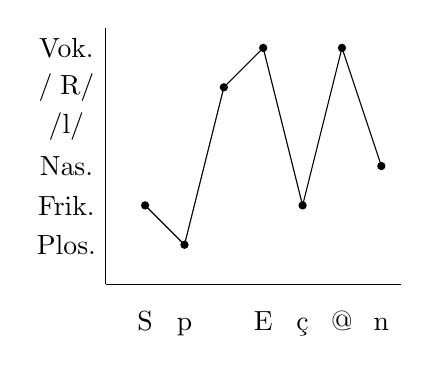
\begin{tikzpicture}[scale=0.5]
\draw[black] (-1,0) -- (6.5,0) ; % x axis
\draw[black] (-1,0) -- (-1,6.5); % y axis
\node at (-2,1) {Plos.};
\node at (-2,2) {Frik.};
\node at (-2,3) {Nas.};
\node at (-2,4) {\textipa{/l/}};
\node at (-2,5) {\textipa{/\;R/}};
\node at (-2,6) {Vok.};
\draw[black] (0,2) -- (1,1) -- (2,5) -- (3,6) -- (4,2) -- (5,6) -- (6,3);
\node at (0,-1) {\strut \textipa{S}};
\node at (1,-1) {\strut \textipa{p}};
\node at (2,-1) {\strut \textipa{\textscr}};
\node at (3,-1) {\strut \textipa{E}};
\node at (4,-1) {\strut \textipa{\c{c}}};
\node at (5,-1) {\strut \textipa{@}};
\node at (6,-1) {\strut \textipa{n}};
\fill (0,2) circle [radius=3pt];
\fill (1,1) circle [radius=3pt];
\fill (2,5) circle [radius=3pt];
\fill (3,6) circle [radius=3pt];
\fill (4,2) circle [radius=3pt];
\fill (5,6) circle [radius=3pt];
\fill (6,3) circle [radius=3pt];
\end{tikzpicture}}}
\end{figure}
\end{minipage}
\pause
\begin{minipage}{.05\textwidth}
\hfill
\end{minipage}
\begin{minipage}{.45\textwidth}
\begin{figure}
\centering
%\visible<4->
{\scalebox{.75}{
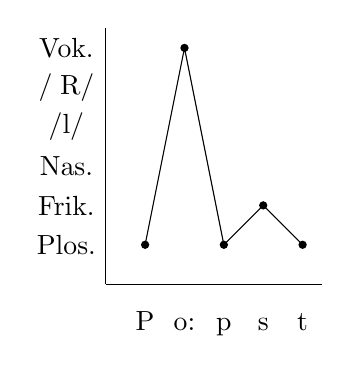
\begin{tikzpicture}[scale=0.5]
\draw[black] (-1,0) -- (4.5,0) ; % x axis
\draw[black] (-1,0) -- (-1,6.5); % y axis
\node at (-2,1) {Plos.};
\node at (-2,2) {Frik.};
\node at (-2,3) {Nas.};
\node at (-2,4) {\textipa{/l/}};
\node at (-2,5) {\textipa{/\;R/}};
\node at (-2,6) {Vok.};
\draw[black] (0,1) -- (1,6) -- (2,1) -- (3,2) -- (4,1);
\node at (0,-1) {\strut \textipa{P}};
\node at (1,-1) {\strut \textipa{o:}};
\node at (2,-1) {\strut \textipa{p}};
\node at (3,-1) {\strut \textipa{s}};
\node at (4,-1) {\strut \textipa{t}};
\fill (0,1) circle [radius=3pt];
\fill (1,6) circle [radius=3pt];
\fill (2,1) circle [radius=3pt];
\fill (3,2) circle [radius=3pt];
\fill (4,1) circle [radius=3pt];
\end{tikzpicture}}}
\end{figure}
\end{minipage}

\end{frame}
%%%%%%%%%%%%%%%%%%%%%%%%%%%%%%%%%

\begin{frame}
\frametitle{Übung -- Lösung}
%
\begin{minipage}{.3\textwidth}
\centering
\scalebox{.75}{\begin{forest} MyP edges, [,phantom
[$\sigma$
[O
[x, tier=word[\textipa{b}]]
[x, tier=word[\textipa{\textscr}]]
]
[R
[N	[x, tier=word[\textipa{a}]]
]
[K
[x[\textipa{n}]]
[x[\textipa{t}]]
]
]  
]
[$\sigma$
[O	[x, tier=word[\textipa{S}]]
]
[R	
[N	
[x[\textipa{U}]]
]
[K	
[x[\textipa{\t{ts}}]]
]
]
]]
\end{forest}}

\end{minipage}
\pause
%
\begin{minipage}{.02\textwidth}
\hfill
\end{minipage}
%
\begin{minipage}{.65\textwidth}
\centering
\scalebox{.75}{
\begin{forest}
MyP edges, [, phantom
[$ \sigma $
[O
[x, tier=word[\textipa{P}]]
]
[R
[N
[x, tier=word[\textipa{a}]]
]
[K
[x[\textipa{p}]]
]
]
]
[$ \sigma $
[O
[x, tier=word[\textipa{S}]]
[x, tier=word[\textipa{t}]]
]
[R
[N
[x[\textipa{a}]]
]
[K
[x[\textipa{n}]]
[x[\textipa{t}]]
[x[\textipa{s}]]
]
]
]
[$ \sigma $
[O
[x, tier=word[\textipa{h}]]
]
[R
[N
[x[\textipa{a}]]
]
[K
[x[\textipa{l}]]
]
]
]
[$ \sigma $
[O
[x, tier=word[t]]
]
[R	
[N
[x[\textipa{\textturna}]]
]
]
]]
\end{forest}}
\end{minipage}
\pause
\begin{minipage}{.3\textwidth}
\begin{figure}
\centering
\scalebox{.75}{
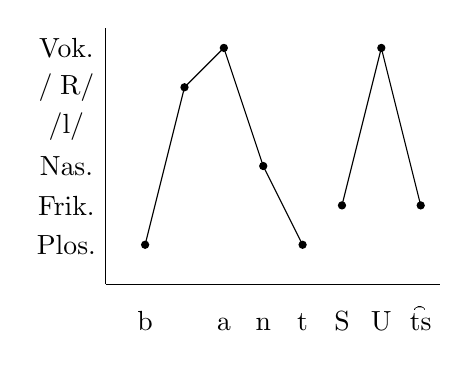
\begin{tikzpicture}[scale=0.5]
\draw[black] (-1,0) -- (7.5,0) ; % x axis
\draw[black] (-1,0) -- (-1,6.5); % y axis
\node at (-2,1) {Plos.};
\node at (-2,2) {Frik.};
\node at (-2,3) {Nas.};
\node at (-2,4) {\textipa{/l/}};
\node at (-2,5) {\textipa{/\;R/}};
\node at (-2,6) {Vok.};
\draw[black] (0,1) -- (1,5) -- (2,6) -- (3,3) -- (4,1);
\draw[black] (5,2) -- (6,6) -- (7,2);
\node at (0,-1) {\strut \textipa{b}};
\node at (1,-1) {\strut \textipa{\textscr}};
\node at (2,-1) {\strut \textipa{a}};
\node at (3,-1) {\strut \textipa{n}};
\node at (4,-1) {\strut \textipa{t}};
\node at (5,-1) {\strut \textipa{S}};
\node at (6,-1) {\strut \textipa{U}};
\node at (7,-1) {\strut \textipa{\t{ts}}};
\fill (0,1) circle [radius=3pt];
\fill (1,5) circle [radius=3pt];
\fill (2,6) circle [radius=3pt];
\fill (3,3) circle [radius=3pt];
\fill (4,1) circle [radius=3pt];
\fill (5,2) circle [radius=3pt];
\fill (6,6) circle [radius=3pt];
\fill (7,2) circle [radius=3pt];
\end{tikzpicture}}
\end{figure}
\end{minipage}
\pause
\begin{minipage}{.05\textwidth}
\hfill
\end{minipage}
\begin{minipage}{.6\textwidth}
\begin{figure}
\centering
\scalebox{.75}{
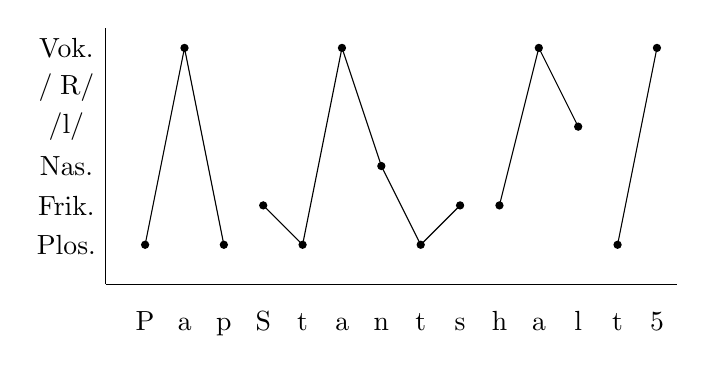
\begin{tikzpicture}[scale=0.5]
\draw[black] (-1,0) -- (13.5,0) ; % x axis
\draw[black] (-1,0) -- (-1,6.5); % y axis
\node at (-2,1) {Plos.};
\node at (-2,2) {Frik.};
\node at (-2,3) {Nas.};
\node at (-2,4) {\textipa{/l/}};
\node at (-2,5) {\textipa{/\;R/}};
\node at (-2,6) {Vok.};
\draw[black] (0,1)--(1,6)--(2,1);
\draw[black](3,2)--(4,1)--(5,6)--(6,3)--(7,1)--(8,2);
\draw[black](9,2)--(10,6)--(11,4);
\draw[black](12,1)--(13,6);
\fill (0,1) circle [radius=3pt];
\fill (1,6) circle [radius=3pt];
\fill (2,1) circle [radius=3pt];
\fill (3,2) circle [radius=3pt];
\fill (4,1) circle [radius=3pt];
\fill (5,6) circle [radius=3pt];
\fill (6,3) circle [radius=3pt];
\fill (7,1) circle [radius=3pt];
\fill (8,2) circle [radius=3pt];
\fill (9,2) circle [radius=3pt];
\fill (10,6) circle [radius=3pt];
\fill (11,4) circle [radius=3pt];
\fill (12,1) circle [radius=3pt];
\fill (13,6) circle [radius=3pt];
\node at (0,-1){\strut \textipa{P}};
\node at (1,-1){\strut \textipa{a}};
\node at (2,-1){\strut \textipa{p}};
\node at (3,-1){\strut \textipa{S}};
\node at (4,-1){\strut \textipa{t}};
\node at (5,-1){\strut \textipa{a}};
\node at (6,-1){\strut \textipa{n}};
\node at (7,-1){\strut \textipa{t}};
\node at (8,-1){\strut \textipa{s}};
\node at (9,-1){\strut \textipa{h}};
\node at (10,-1){\strut \textipa{a}};
\node at (11,-1){\strut \textipa{l}};
\node at (12,-1){\strut \textipa{t}};
\node at (13,-1){\strut \textipa{5}};
\end{tikzpicture}}
\end{figure}
\end{minipage}


\end{frame}

}

%%%%%%%%%%%%%%%%%%%%%%%%%%%%%%%%%%


%%%%%%%%%%%%%%%%%%%%%%%%%%%%%%%%%%
\subsection{Silbifizierung}

%% MyP: Contents
\iftoggle{sectoc}{
	\frame{
		%\begin{multicols}{2}
		\frametitle{~}
		\tableofcontents[currentsubsection, subsubsectionstyle=hide]
		%\end{multicols}
	}
}

%% StM: Contents
\iftoggle{gliederung}{
	
	\outline{
		\begin{itemize}
			
			\item Silbenmodelle
			%% CV-Modell
			%% Konstituentenmodell
			\item Silbengelenk
			\item \blaubf{Silbifizierung}
			\item Exkurs: Akzent
			\item Hausaufgabe
			
		\end{itemize}
	}
}
%%%%%%%%%%%%%%%%%%%%%%%%%%%%%%%%%%

\begin{frame}
\frametitle{Silbifizierung}

\begin{block}{Silbifizierung (auch Syllabierung)}
	Wörter in Silben einteilen
\end{block}

\begin{itemize}
	\item Wie würden Sie folgende Lautsequenzen silbifizieren?
	
	\ea ata, odo, eke
	\z
	
	\pause
	
	\item Ein einziger intervokalischer Konsonant wird immer als Silbenanlaut silbifiziert (universelles Prinzip: \textbf{Onset-Maximierung}).


\end{itemize}

\begin{block}{Onset-Maximierung}
Bilde zuerst den größtmöglichen Silbenanlaut;\\
dann bilde den Silbenauslaut \citep[218]{Hall00a}.
\end{block}

\end{frame}


%%%%%%%%%%%%%%%%%%%%%%%%%%%%%%%%%%
\begin{frame}
\frametitle{Onset-Maximierung}

\begin{block}{Onset-Maximierung}
Bilde zuerst den größtmöglichen Silbenanlaut;\\
dann bilde den Silbenauslaut \citep[218]{Hall00a}.
\end{block}


\begin{itemize}
\item Onset-Maximierung herleitbar aus:
\begin{enumerate}
\item Silbenanlautgesetz (CV häufiger als V), und
\item Silbenauslautgesetz (CVC$^{n} >$ CVC$^{n+1}$, wobei $n \geq 0$)
\end{enumerate}

\pause
\item Silbifizierung nicht über Morphemgrenzen hinweg! 
\item Ausnahme: Suffixe mit vokalischem Onset:

\ea
kind\#isch: \textipa{[kIn.dIS]}

\ex
kind\#lich: \textipa{[kInt.lI\c{c}]}
\z

\item \# := Morphemgrenze

% Wenn man Morphmgrenzenbedingung weglassen würde, ergäbe sich Bra. ndschutz

% rek.nen vs. re.gnen

\end{itemize}

\end{frame}


%%%%%%%%%%%%%%%%%%%%%%%%%%%%%%%%%%
%\subsection{Übung}
%
%%% MyP: Contents
%\iftoggle{sectoc}{
%	\frame{
%		%\begin{multicols}{2}
%		\frametitle{~}
%		\tableofcontents[currentsubsection, subsubsectionstyle=hide]
%		%\end{multicols}
%	}
%}
%%%%%%%%%%%%%%%%%%%%%%%%%%%%%%%%%%
\begin{frame}
\frametitle{Übung}

\begin{itemize}
	\item Was bedeutet die Annahme des Sonoritätsprinzips und der Onset-Maximierung für die folgenden Beispielwörter?
	
	\eal\label{ex:fabrik}
	\ex Fabrik
	\ex Imker
	\ex neblig
	\ex Falter
	\ex regnen
	\zl
\end{itemize}

\end{frame}


%%%%%%%%%%%%%%%%%%%%%%%%%%%%%%%%
\iftoggle{ue-loesung}{
	%%%%%%%%%%%%%%%%%%%%%%%%%%%%%%%%%%
%% UE 1 - 03c Phonologie
%%%%%%%%%%%%%%%%%%%%%%%%%%%%%%%%%%


\begin{frame}
\frametitle{Übung -- Lösung}

\begin{itemize}
	\item Was bedeutet die Annahme des Sonoritätsprinzips und der Onset-Maximierung für die folgenden Beispielwörter:
	
	\begin{exe}
	\exr{ex:fabrik}
	\settowidth\jamwidth{XXXXXXXXXXXXXXXXXXXXXXXXXXXXXXXXXXXX}
	\begin{xlist}
		\ex Fabrik\loesung{1}{\textipa{[fa.b\textscr ik]} (auch: \textipa{[fa.b\;Ri:k]} oder \textipa{[fa.b\;RIk]})}
		\ex Imker\loesung{2}{\textipa{[PIm.k5]}}
		\ex neblig\loesung{3}{\textipa{[ne:.blI\c{c}]}}
		\ex Falter\loesung{4}{\textipa{[fal.t5]}}
		\ex regnen\loesung{5}{\textipa{[\textscr e:.gn@n]}}
		
	\loesung{6}{Koda: *Obstruent vor Sonorant}
	\loesung{7}{Onset: *Sonorant vor Obstruent}
	
	\end{xlist}
\end{exe}
	
	\alertred{Onset-Maximierung ist nicht strikt. Alternativ ginge auch \textipa{[ne:p.lI\c{c}]}, \textipa{[\textscr e:k.n@n]}.}
	
\end{itemize}

\end{frame}	

}

%%%%%%%%%%%%%%%%%%%%%%%%%%%%%%%
\begin{frame}{Übung}

\begin{itemize}
	\item Welche Prinzipien bzw. Regularitäten werden verletzt bei:


	\eal\label{ex:ebbe}
	\ex \textipa{[PE.b@]}
	\ex \textipa{[PEb.@]}
	\ex \textipa{[PEp.@]}
	\ex \textipa{[PEp.b@]}
	\zl
	
\end{itemize}

\end{frame}


%%%%%%%%%%%%%%%%%%%%%%%%%%%%%%%%
\iftoggle{ue-loesung}{
	%%%%%%%%%%%%%%%%%%%%%%%%%%%%%%%%%%
%% UE 2 - 03c Phonologie
%%%%%%%%%%%%%%%%%%%%%%%%%%%%%%%%%%

\begin{frame}
\frametitle{Übung -- Lösung}
	\begin{itemize}

	\item Welche Prinzipien bzw. Regularitäten werden verletzt bei:


	\eal
	\settowidth\jamwidth{XXXXXXXXXXXXXXXXXXXXXXXXXXXXXXXXXXXX}
	
		\ex \textipa{[PE.b@]}\jambox{\only<1->{\textcolor{red}{
			\ras Kurzvokal} Lösung \zb Silbengelenk \textipa{[PE\.b@]}
		}}
		\ex \textipa{[PEb.@]}\loesung{2}{\ras Auslautverhärtung}
		\ex \textipa{[PEp.@]}\loesung{3}{\ras Onset-Maximierung}
		\ex \textipa{[PEp.b@]}\loesung{4}{\ras keine Regelverletzung}
	\zl

	\end{itemize}

\end{frame}

}

%%%%%%%%%%%%%%%%%%%%%%%%%%%%%%%
\begin{frame}
\frametitle{Übung}

\begin{itemize}
	\item Silbifizieren Sie folgende Segmentsequenzen \textbf{in zwei Schritten}:
	\begin{itemize}
		\item Onset-Maximierungsprinzip
		\item Sonoritätsprinzip
	\end{itemize}
	
	\item Stellen Sie fest, ob alle Silben wohlgeformt sind.\\
	Falls nicht, benennen Sie die Verletzungen.
	
	\ea\label{ex:otling}
	\textipa{[o:tlIN5mSplag\textscr e:hOn]}
	\z
	
	% Otlingamsplagrehon
	
	\ea\label{ex:blumen}
	Blumentopferde
	\z
	
\end{itemize}

% blu.men.to.pfer.de

%\ea
%Urinstinkt
%\z	

\end{frame}


%%%%%%%%%%%%%%%%%%%%%%%%%%%%%%%%%%
\iftoggle{ue-loesung}{
	%%%%%%%%%%%%%%%%%%%%%%%%%%%%%%%%%%
%% UE 3 - 03c Phonologie
%%%%%%%%%%%%%%%%%%%%%%%%%%%%%%%%%%

\begin{frame}
\frametitle{Übung -- Lösung}

\begin{itemize}
\item Silbifizieren Sie folgende Segmentsequenzen \textbf{in zwei Schritten}:
\begin{itemize}
	\item Onsetmaximierungsprinzip
	\item Sonoritätsprinzip
\end{itemize}

\item Stellen Sie fest, ob alle Silben wohlgeformt sind.\\
Falls nicht, benennen Sie die Verletzungen.

\begin{exe}
	\exr{ex:otling}
	\textipa{[o:tlIN5mSplag\textscr e:hOn]}\\
	\alertred{zuerst Onset"=Maximierung: \textipa{o: . tlI . \ng {\textturna} . mSpla . g\textscr e: . hOn}\\
	dann Anwendung des Sonoritätsprinzips: \textipa{o: . tlI\. \ng \textturna mS . pla . g\textscr e: . hOn}}
\end{exe}

% Otlingamsplagrehon

\begin{exe}
	\exr{ex:blumen}
	Blumentopferde\\ \pause
	\alertred{zuerst Onset-Maximierung: \textipa{blu: . m@ . ntO . pfE . {\textscr}d@}\\
	dann Awendung des Sonoritätsprinzips: \textipa{blu: . m@n . tO . pfE{\textscr} . d@}}
\end{exe}

\end{itemize}

% blu.men.to.pfer.de

%\ea
%Urinstinkt
%\z	

\end{frame}


% ' Stahl , tische     Hauptbetonung auf Stahl, Nebenbetonung auf Tische


}

%%%%%%%%%%%%%%%%%%%%%%%%%%%%%%%%%%


%%%%%%%%%%%%%%%%%%%%%%%%%%%%%%%%%%
\subsection{Exkurs: Akzent}
%%%%%%%%%%%%%%%%%%%%%%%%%%%%%%%%%%

%% MyP: Contents
\iftoggle{sectoc}{
	\frame{
		%\begin{multicols}{2}
		\frametitle{~}
		\tableofcontents[currentsubsection, subsubsectionstyle=hide]
		%\end{multicols}
	}
}

%% StM: Contents
\iftoggle{gliederung}{
	
	\outline{
		\begin{itemize}
			
			\item Silbenmodelle
			%% CV-Modell
			%% Konstituentenmodell
			\item Silbengelenk
			\item Silbifizierung
			\item \blaubf{Exkurs: Akzent}
			\item Hausaufgabe
			
		\end{itemize}
	}
}
%%%%%%%%%%%%%%%%%%%%%%%%%%%%%%%%%%

\begin{frame}
\frametitle{Exkurs: Akzent}

\begin{itemize}
\item Silben können \textbf{betont} oder \textbf{unbetont} sein, d.\,h. sie können einen Akzent tragen oder nicht.
\item[]

\begin{block}{Akzent}
\textbf{Auditiver Eindruck der Prominenz eines Vokals} gegenüber einem anderen durch (relational, nicht absolut!):
\begin{itemize}
\item Lautstärke
\item Dauer
\item Höhere Tonlage
\item Ausgeprägtere Artikulationsbewegungen
\end{itemize}
\end{block}	 

\item[]
\item Man unterscheidet zwischen \textbf{Wort-} und \textbf{Satzakzent} (engl. \emph{stress} und \emph{accent}).

\end{itemize}

\end{frame}



%%%%%%%%%%%%%%%%%%%%%%%%%%%%%%%%%%%
%%%%%%%%%%%%%%%%%%%%%%%%%%%%%%%%%%
%\subsubsection{Exkurs: Wortakzent}
%\frame{
%\begin{multicols}{2}
%\frametitle{~}
%	\tableofcontents[currentsection]
%\end{multicols}
%}
%%%%%%%%%%%%%%%%%%%%%%%%%%%%%%%%%%

\begin{frame}
\frametitle{Exkurs: Wortakzent}

\begin{itemize}
\item Was scheint die häufigste Betonung im Deutschen zu sein?

\ea
Mutter, Männer, Autos, Hühner, Lehrer, Kinder, alle, \ldots
\z

\pause
\textbf{betont-unbetont (Trochäus)}

\item Ausnahmen (die je nach Theorie verschieden erklärt werden):

\end{itemize}

\begin{minipage}{.4\textwidth}

\eal 
\ex \textipa{['f\textscr aU]}
\ex \textipa{[mu.'zi:k]}
\ex \textipa{['le:.b@n.d@]}
\ex \textipa{[pa.pa.'g\t{aɪ}]}
\ex \textipa{[f\t{ɛɐ}.'Pa\textscr .b\t{aɪ}.t@n]}
\zl

\end{minipage}
\begin{minipage}{.5\textwidth}

%	\iftoggle{loesung}{
\begin{itemize}
\item[] \textcolor{red}{\ras nur eine Silbe }
\item[] \textcolor{red}{\ras Fremdwort}
\item [] \textcolor{red}{\ras Flektierte Elemente \ab{-de}}
\item [] \textcolor{red}{\ras Fremdwort}
\item [] \textcolor{red}{\ras Derivation \ab{ver-}}
\end{itemize}
%}

\end{minipage}

\end{frame}



%%%%%%%%%%%%%%%%%%%%%%%%%%%%%%%%%%%
%%%%%%%%%%%%%%%%%%%%%%%%%%%%%%%%%%
%\subsubsection{Exkurs: Satzakzent}
%\frame{
%\begin{multicols}{2}
%\frametitle{~}
%	\tableofcontents[currentsection]
%\end{multicols}
%}
%%%%%%%%%%%%%%%%%%%%%%%%%%%%%%%%%%

\begin{frame}
\frametitle{Exkurs: Satzakzent}

\begin{itemize}
\item In einem Satz können betonte Silben \textbf{noch weiter hervorgehoben} werden (dabei meist durch die Tonhöhe):

\eal 
\ex Géstern hat BÁyern gewónnen.
\ex GÉStern hat Báyern gewónnen.
\ex Géstern hat Báyern geWÓNnen.
\zl
\item Die prominenteste Silbe im Satz wird meist mit \textbf{Großbuchstaben} dargestellt, sie trägt den Satzakzent.

\item Durch diese Akzentuierung wird das gesamte Wort
hervorgehoben.\\
\ras \textbf{Fokus des Satzes} (\gqq{Informationsstruktur})

\end{itemize}

\end{frame}



%%%%%%%%%%%%%%%%%%%%%%%%%%%%%%%%%%%
%%%%%%%%%%%%%%%%%%%%%%%%%%%%%%%%%%
%\subsubsection{Exkurs: Intonation}
%\frame{
%\begin{multicols}{2}
%\frametitle{~}
%	\tableofcontents[currentsection]
%\end{multicols}
%}
%%%%%%%%%%%%%%%%%%%%%%%%%%%%%%%%%%

\begin{frame}
\frametitle{Exkurs: Intonation}

\begin{block}{Intonation}
Tonhöhenverlauf (\gqq{Melodie}) einer Äußerung
\end{block}

\begin{itemize}
\item \textbf{Satztypen} können mittels Intonation unterschieden werden.

\item Sprechen Sie die folgenden Äußerungen mit fallender und steigender Intonation.
\eal 
\ex Heute gewinnen die Bayern.
\ex Schon Schluss.
\zl
\pause
\textbf{Aussage-} \vs \textbf{Interrogativsatz}	

\end{itemize}

\end{frame}



%%%%%%%%%%%%%%%%%%%%%%%%%%%%%%%%%%

\begin{frame}
\frametitle{Disambiguierung}

Ambige ($\approx$ mehrdeutige) Sätze können mittels Intonation \gs{durch die sog. Hutkontur} \textbf{disambiguiert} werden: 

\begin{exe}
\ex  \label{exe:nicht}Alle Studenten haben die Klausur nicht bestanden.

	\begin{xlist}
	\ex Es ist nicht der Fall, dass alle Studenten die Klausur bestanden haben. \hfill $\lsem \neg \forall \rsem$
	\ex Für alle Studenten gilt, dass sie die Klausur nicht bestanden haben. \hfill $\lsem \forall \neg \rsem$
	\end{xlist}

\pause 

\ex /ALle Studenten haben die Klausur  NICHT\textbackslash\ bestanden.
\exr{exe:nicht}
	\begin{xlist}
	\ex Es ist nicht der Fall, dass alle Studenten die Klausur bestanden haben. \hfill $\lsem \neg \forall \rsem$
	\end{xlist}
\end{exe}


\end{frame}


%%%%%%%%%%%%%%%%%%%%%%%%%%%%%%%%%%
\subsection{Hausaufgabe}
%%%%%%%%%%%%%%%%%%%%%%%%%%%%%%%%%%

%%% MyP: Contents
%\iftoggle{sectoc}{
%	\frame{
%		%\begin{multicols}{2}
%		\frametitle{~}
%		\tableofcontents[currentsubsection, subsubsectionstyle=hide]
%		%\end{multicols}
%	}
%}

%%% StM: Contents
%\iftoggle{gliederung}{
%	
%	\outline{
%		\begin{itemize}
%			
%			\item Silbenmodelle
%			%% CV-Modell
%			%% Konstituentenmodell
%			\item Silbengelenk
%			\item Silbifizierung
%			\item Exkurs: Akzent
%			\item \blaubf{Hausaufgabe}
%			
%		\end{itemize}
%	}
%}


%%%%%%%%%%%%%%%%%%%%%%%%%%%%%%%%%%
\begin{frame}%[allowframebreaks]
\frametitle{Hausaufgabe}
\begin{itemize}

\item[1.] Geben Sie eine \textbf{phonetische Transkription} der folgenden Wörter nach der \gqq{Standardaussprache} an, zeichnen Sie dabei die \textbf{Silbenstruktur} nach dem \textbf{Konstituentenmodell} und mit der \textbf{Skelettschicht} und geben Sie die \textbf{Sonoritätsprofile} an.

\eal\label{ex:03cHA1}
\ex Stimmenfang \label{ex:03cHA1a}
\ex Mittagessen\label{ex:03cHA1b}
\ex Bierdeckel\label{ex:03cHA1c}
\zl
\end{itemize}

\begin{block}{Sonoritätshierarchie (Zur Erinnerung)}
Vokal $>$ \textipa{/\textscr /} $>$ \textipa{/l/} $>$ Nasal $>$ Frikativ $>$ Plosiv \\
$x > y$ := $x$ ist sonorer als $y$
\end{block}

\end{frame}

%%%%%%%%%%%%%%%%%%%%%%%%%%%%%%%%%%%%%%%%%%%%%%%%%%%%%

\begin{frame}
\begin{itemize}
\item[2.] Silbifizieren Sie folgende Segmentsequenzen \textbf{in zwei Schritten}:
\begin{itemize}
\item Onset-Maximierungsprinzip
\item Sonoritätsprinzip
\end{itemize}

Stellen Sie fest, ob alle Silben wohlgeformt sind. Falls nicht, benennen Sie die Verletzungen.
\ea\label{ex:03cHA2}
Urinstinkt
\z	
\item[3.] Geben Sie die standarddeutsche \textbf{phonetische Transkription} des Wortes \ab{Stahltische} inklusive der \textbf{Silbenstruktur} (mit X-Skelettschicht) an.\\Ermitteln Sie die \textbf{Kriterien}, die bei der Silbifizierung wirken.

\item[4.] Geben Sie die Gründe an, warum die folgenden Wörter aus phonetisch"=phonologischen Gründen im Deutschen nicht möglich sind:

\eal\label{ex:03cHA3}
\ex[*]{\textipa{['Napl.O:t]}}
\ex[*]{\textipa{[a\;R.'tUng]}}
\zl

\end{itemize}

\end{frame}

%%%%%%%%%%%%%%%%%%%%%%%%%%%%%%%%%%%
\iftoggle{ha-loesung}{
	%%%%%%%%%%%%%%%%%%%%%%%%%%%%%%%%%%
%% HA 1 - 03c Phonologie
%%%%%%%%%%%%%%%%%%%%%%%%%%%%%%%%%%

\begin{frame}%[allowframebreaks]
\frametitle{Hausaufgabe -- Lösung}
\begin{itemize}

\item[1.] Geben Sie eine \textbf{phonetische Transkription} der folgenden Wörter nach der \gqq{Standardaussprache} an, zeichnen Sie dabei die \textbf{Silbestruktur} nach dem \textbf{Konstituentenmodell} und mit der \textbf{Skelettschicht} und geben Sie die \textbf{Sonoritätsprofile} an.

\begin{exe}
\exi{(\ref{ex:03cHA1})}
\begin{xlist}
\ex Stimmenfang
\ex Mittagessen
\ex Bierdeckel
\end{xlist}
\end{exe}

\begin{block}{Sonoritätshierarchie (Zur Erinnerung)}
Vokal $>$ \textipa{/\textscr /} $>$ \textipa{/l/} $>$ Nasal $>$ Frikativ $>$ Plosiv \\
$x > y :=$ $x$ ist sonorer als $y$
\end{block}

\end{itemize}
\end{frame}
%%%%%%%%%%%%%%%%%%%%%%%%%%%%%%%%%%

\begin{frame}{Hausaufgabe -- Lösung}

Zu (\ref{ex:03cHA1a}):

\begin{columns}	
	
\column[b]{.5\textwidth}

\begin{figure}
%	\footnotesize
	\centering
	\begin{forest} MyP edges, [, phantom
		[$\sigma$
		[O [x, tier=word [\textipa{S}]] [x, tier=word [\textipa{t}]]]
		[R [N [x, tier=word [\textipa{I}]]] [K [x, name=x [\textipa{m}]]]]
		]
		[$\sigma$
		[O, name=onset]
		[R [N [x [\textipa{@}]]] [K [x [\textipa{n}]]]]
		]
		[$\sigma$
		[O [x, tier=word [\textipa{f}]]]
		[R [N [x [\textipa{a}]]] [K [x [\textipa{N}]]]]
		]
		]				
		{
		\draw[black] (x.north)--(onset.south);
		}
	\end{forest}
\end{figure}

\pause

\column[b]{.5\textwidth}

\begin{figure}
%	\footnotesize
	\centering	
	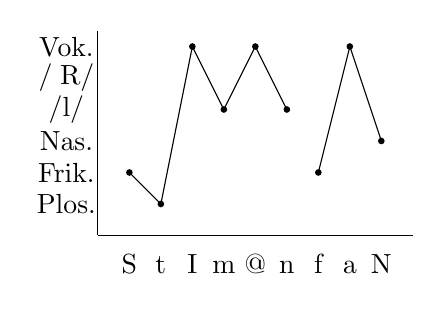
\begin{tikzpicture}[scale=0.4]
		\draw[black] (-1,0) -- (9,0) ; % x axis
		\draw[black] (-1,0) -- (-1,6.5); % y axis
		\node at (-2,1) {Plos.};
		\node at (-2,2) {Frik.};
		\node at (-2,3) {Nas.};
		\node at (-2,4) {\textipa{/l/}};
		\node at (-2,5) {\textipa{/\;R/}};
		\node at (-2,6) {Vok.};
		\draw[black] (0,2) -- (1,1) -- (2,6) -- (3,4) -- (4,6) -- (5,4);
		\draw[black] (6,2) -- (7,6) -- (8,3);
		\node at (0,-1) {\strut \textipa{S}};
		\node at (1,-1) {\strut \textipa{t}};
		\node at (2,-1) {\strut \textipa{I}};
		\node at (3,-1) {\strut \textipa{m}};
		\node at (4,-1) {\strut \textipa{@}};
		\node at (5,-1) {\strut \textipa{n}};
		\node at (6,-1) {\strut \textipa{f}};
		\node at (7,-1) {\strut \textipa{a}};
		\node at (8,-1) {\strut \textipa{N}};
		\fill (0,2) circle [radius=3pt];
		\fill (1,1) circle [radius=3pt];
		\fill (2,6) circle [radius=3pt];
		\fill (3,4) circle [radius=3pt];
		\fill (4,6) circle [radius=3pt];
		\fill (5,4) circle [radius=3pt];
		\fill (6,2) circle [radius=3pt];
		\fill (7,6) circle [radius=3pt];
		\fill (8,3) circle [radius=3pt];
	\end{tikzpicture}
\end{figure}

\end{columns}

\end{frame}


%%%%%%%%%%%%%%%%%%%%%%%%%%%%%%%%%%%%%%%%%%%%%%%
\begin{frame}{Hausaufgabe -- Lösung}


Zu (\ref{ex:03cHA1b})

\begin{columns}
	\column[b]{.5\textwidth}
	
\begin{figure}
\footnotesize
\centering
	\begin{forest} MyP edges, [, phantom
		[$\sigma$
		[O [x, tier=word [\textipa{m}]]] 
		[R [N [x, tier=word [\textipa{I}]]] [K [x, name=x1 [\textipa{t}]]]]
		]
		[$\sigma$
		[O, name=onset1]
		[R [N [x [\textipa{a:}, name=a]]
		[x, name=ax]] [K [x [\textipa{k}]]]]
		]
		[$\sigma$
		[O [x, tier=word [\textipa{P}]]]
		[R [N [x [\textipa{E}]]] [K [x, name=x2 [\textipa{s}]]]]
		]
		[$\sigma$
		[O, name=onset2]
		[R [N [x [\textipa{\textsyllabic{n}}]]]
		]
		]]
		{
		\draw[black] (x1.north)--(onset1.south);
		\draw[black] (x2.north)--(onset2.south);
		\draw[black] (a.north)--(ax.south);
		}
	\end{forest}
\end{figure}

\pause
\column[b]{.5\textwidth}

\begin{figure}
	\footnotesize
	\centering
	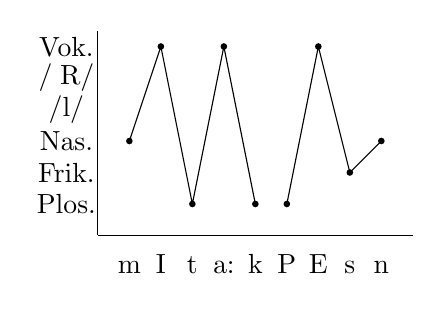
\begin{tikzpicture}[scale=0.4]
		\draw[black] (-1,0) -- (9,0) ; % x axis
		\draw[black] (-1,0) -- (-1,6.5); % y axis
		\node at (-2,1) {Plos.};
		\node at (-2,2) {Frik.};
		\node at (-2,3) {Nas.};
		\node at (-2,4) {\textipa{/l/}};
		\node at (-2,5) {\textipa{/\;R/}};
		\node at (-2,6) {Vok.};
		\draw[black] (0,3) -- (1,6) -- (2,1) -- (3,6) -- (4,1);
		\draw[black] (5,1) -- (6,6) -- (7,2) -- (8,3);
		\node at (0,-1) {\strut \textipa{m}};
		\node at (1,-1) {\strut \textipa{I}};
		\node at (2,-1) {\strut \textipa{t}};
		\node at (3,-1) {\strut \textipa{a:}};
		\node at (4,-1) {\strut \textipa{k}};
		\node at (5,-1) {\strut \textipa{P}};
		\node at (6,-1) {\strut \textipa{E}};
		\node at (7,-1) {\strut \textipa{s}};
		\node at (8,-1) {\strut \textipa{\textsyllabic{n}}};
		\fill (0,3) circle [radius=3pt];
		\fill (1,6) circle [radius=3pt];
		\fill (2,1) circle [radius=3pt];
		\fill (3,6) circle [radius=3pt];
		\fill (4,1) circle [radius=3pt];
		\fill (5,1) circle [radius=3pt];
		\fill (6,6) circle [radius=3pt];
		\fill (7,2) circle [radius=3pt];
		\fill (8,3) circle [radius=3pt];
	\end{tikzpicture}
\end{figure}

\end{columns}

\end{frame}


%%%%%%%%%%%%%%%%%%%%%%%%%%%%%%%%%%%%%%%%%%%%
\begin{frame}{Hausaufgabe -- Lösung}

Zu (\ref{ex:03cHA1b})  (alternative Lösung):

\begin{columns}
	\column[b]{.5\textwidth}
	
	
\begin{figure}
\footnotesize
\centering

	\begin{forest} MyP edges, [, phantom
		[$\sigma$
		[O [x, tier=word [\textipa{m}]]] 
		[R [N [x, tier=word [\textipa{I}]]] [K [x, name=x1 [\textipa{t}]]]]
		]
		[$\sigma$
		[O, name=onset1]
		[R [N [x [\textipa{a:}, name=a]]
		[x, name=ax]] [K [x [\textipa{k}]]]]
		]
		[$\sigma$
		[O [x, tier=word [\textipa{P}]]]
		[R [N [x [\textipa{E}]]] [K [x, name=x2 [\textipa{s}]]]]
		]
		[$\sigma$
		[O, name=onset2]
		[R [N [x [\textipa{@}]]] [K [x [\textipa{n}]]]]
		]
		]
		{
		\draw[black] (x1.north)--(onset1.south);
		\draw[black] (x2.north)--(onset2.south);
		\draw[black] (a.north)--(ax.south);
		}
	\end{forest}

\end{figure}

\pause

\column[b]{.5\textwidth}

\begin{figure}
\footnotesize
\centering
	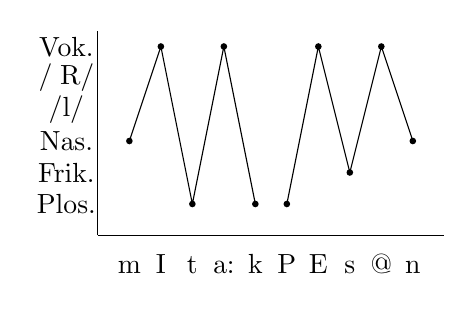
\begin{tikzpicture}[scale=0.4]
		\draw[black] (-1,0) -- (10,0) ; % x axis
		\draw[black] (-1,0) -- (-1,6.5); % y axis
		\node at (-2,1) {Plos.};
		\node at (-2,2) {Frik.};
		\node at (-2,3) {Nas.};
		\node at (-2,4) {\textipa{/l/}};
		\node at (-2,5) {\textipa{/\;R/}};
		\node at (-2,6) {Vok.};
		\draw[black] (0,3) -- (1,6) -- (2,1) -- (3,6) -- (4,1);
		\draw[black] (5,1) -- (6,6) -- (7,2) -- (8,6) -- (9,3);
		\node at (0,-1) {\strut \textipa{m}};
		\node at (1,-1) {\strut \textipa{I}};
		\node at (2,-1) {\strut \textipa{t}};
		\node at (3,-1) {\strut \textipa{a:}};
		\node at (4,-1) {\strut \textipa{k}};
		\node at (5,-1) {\strut \textipa{P}};
		\node at (6,-1) {\strut \textipa{E}};
		\node at (7,-1) {\strut \textipa{s}};
		\node at (8,-1) {\strut \textipa{@}};
		\node at (9,-1) {\strut \textipa{n}};
		\fill (0,3) circle [radius=3pt];
		\fill (1,6) circle [radius=3pt];
		\fill (2,1) circle [radius=3pt];
		\fill (3,6) circle [radius=3pt];
		\fill (4,1) circle [radius=3pt];
		\fill (5,1) circle [radius=3pt];
		\fill (6,6) circle [radius=3pt];
		\fill (7,2) circle [radius=3pt];
		\fill (8,6) circle [radius=3pt];
		\fill (9,3) circle [radius=3pt];
	\end{tikzpicture}
\end{figure}

\end{columns}

\end{frame}


%%%%%%%%%%%%%%%%%%%%%%%%%%%%%%%%%%%%%%%%%%%%%%%
\begin{frame}{Hausaufgabe -- Lösung}

Zu (\ref{ex:03cHA1c}):

\begin{columns}
	\column[b]{.5\textwidth}
	
\begin{figure}
\centering
	\begin{forest} MyP edges, [, phantom
		[$\sigma$
		[O [x,tier=word [\textipa{b}]]]
		[R [N [x, tier=word [\textipa{i:}, name=i]] [x,name=x1]] [K [x [\textipa{5}]]]]
		]
		[$\sigma$
		[O [x, tier=word [\textipa{d}]]]
		[R [N [x [\textipa{E}]]] [K [x, name=x [\textipa{k}]]]]
		]
		[$\sigma$
		[O, name=onset]
		[R [N [x, tier=word [\textipa{@}]]] [K [x [\textipa{l}]]]]
		]
		]
		{
		\draw[black] (x1.south)--(i.north);
		\draw[black] (x.north)--(onset.south);
		}
	\end{forest}
\end{figure}

\pause

\column[b]{.5\textwidth}

\begin{figure}
\centering
	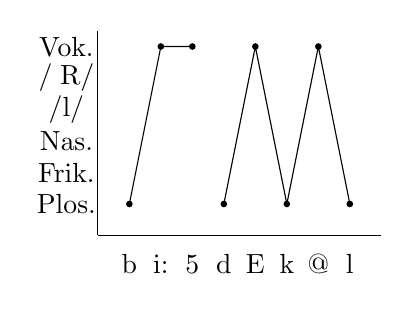
\begin{tikzpicture}[scale=0.4]
		\draw[black] (-1,0) -- (8,0) ; % x axis
		\draw[black] (-1,0) -- (-1,6.5); % y axis
		\node at (-2,1) {Plos.};
		\node at (-2,2) {Frik.};
		\node at (-2,3) {Nas.};
		\node at (-2,4) {\textipa{/l/}};
		\node at (-2,5) {\textipa{/\;R/}};
		\node at (-2,6) {Vok.};
		\draw[black] (0,1) -- (1,6) -- (2,6);
		\draw[black] (3,1) -- (4,6) -- (5,1) -- (6,6) -- (7,1);
		\node at (0,-1) {\strut \textipa{b}};
		\node at (1,-1) {\strut \textipa{i:}};
		\node at (2,-1) {\strut \textipa{5}};
		\node at (3,-1) {\strut \textipa{d}};
		\node at (4,-1) {\strut \textipa{E}};
		\node at (5,-1) {\strut \textipa{k}};
		\node at (6,-1) {\strut \textipa{@}};
		\node at (7,-1) {\strut \textipa{l}};
		\fill (0,1) circle [radius=3pt];
		\fill (1,6) circle [radius=3pt];
		\fill (2,6) circle [radius=3pt];
		\fill (3,1) circle [radius=3pt];
		\fill (4,6) circle [radius=3pt];
		\fill (5,1) circle [radius=3pt];
		\fill (6,6) circle [radius=3pt];
		\fill (7,1) circle [radius=3pt];
	\end{tikzpicture}
\end{figure}

\end{columns}

\end{frame}


%%%%%%%%%%%%%%%%%%%%%%%%%%%%%%%%%%%%%%%%%%%%%%%%%%%
\begin{frame}{Hausaufgabe -- Lösung}
\begin{itemize}
\item[2.] Silbifizieren Sie folgende Segmentsequenzen \textbf{in zwei Schritten}:
\begin{itemize}
\item Onsetmaximierungsprinzip
\item Sonoritätsprinzip
\end{itemize}

Stellen Sie fest, ob alle Silben wohlgeformt sind.\\
Falls nicht, benennen Sie die Verletzungen.

\begin{exe}
\exr{ex:03cHA2} Urinstinkt
\pause
\begin{xlist}
	\ex \alertred{\textipa{[Pu.\;RI.nStInkt]} (Onsetmaximierung)} \pause
	\ex  \alertred{\textipa{[Pu.\;RIn.(\,S\,)tInkt]} (Sonoritätsprinzip, \textipa{S} ist extrasilbisch)} \pause
	\ex  \alertred{\textipa{[Pu5.PIn.stinkt]} (Silbifizierung)}
\end{xlist}
\end{exe}
\pause

\item (\ref{ex:03cHA2}a) und (\ref{ex:03cHA2}b) sind einfach nach der Lautfolge silbifiziert.\\
Silbifizierung erfolgt jedoch auf der Ebene des phonologischen Wortes.\\
Daher werden die phonologischen Wörter \ab{ur-} und \ab{Instinkt} einzeln silbifiziert.
\end{itemize}
\end{frame}

%%%%%%%%%%%%%%%%%%%%%%%%%%%%%%%%%%%%%%%%%%%%%%%%

\begin{frame}{Hausaufgabe -- Lösung}
\begin{itemize}	
\item[3.] Geben Sie die standarddeutsche \textbf{phonetische Transkription} des Wortes \ab{Stahltische} inklusive der \textbf{Silbenstruktur} (mit X-Skelettschicht) an. Ermitteln Sie die \textbf{Kriterien}, die bei der Silbifizierung wirken.
\end{itemize}

\pause

\begin{minipage}{.5\textwidth}
\begin{figure}
\scalebox{.8}{\begin{forest}
MyP edges [, phantom
[$\sigma$
[O 
[x, tier=word[\textipa{S}]]
[x, tier=word[\textipa{t}]]
]
[R
[N
[x, tier=word[\textipa{a:}, name=a]]
[x, name=x]
]
[K[x[\textipa{l}]]]
]
]
[$\sigma$
[O [x, tier=word[\textipa{t}]]]
[R
[N
[x[\textipa{I}]]
]
[K
[x,name=S[\textipa{S}] ]
]
]
]
[$\sigma$
[O, name=o]
[R
[N
[x[\textipa{@}]]
]
]
]
]
\draw[black](o.south)--(S.north);
\draw[black](a.north)--(x.south);
\end{forest}}
\end{figure}
\end{minipage}
\begin{minipage}{.45\textwidth}
	
\pause	
	
\begin{itemize}
\item Onset-Maximierung \pause
\item Sonoritätshierarchie im Onset: *Sonorant vor Obstruent (*[\textipa{lt}]) \pause
\item Silbengelenk nach ungespanntem, betontem Vokal
\end{itemize}
\end{minipage}

\end{frame}

%%%%%%%%%%%%%%%%%%%%%%%%%%%%%%%%%%%%%

\begin{frame}{Hausaufgabe -- Lösung}
\begin{itemize}

\item[4.] Geben Sie die Gründe an, warum die folgenden Wörter aus phonetisch/""phonologischen Gründen im Deutschen nicht möglich sind:

\begin{exe}
	\exr{ex:03cHA3}
	\settowidth\jamwidth{XXXXXXXXXXXXXXXXXXXXXXXXXXXXXXXXXXX}
	\begin{xlist}
		\ex[*]{ \textipa{['Napl.O:t]}
			\loesung{2}{Onset-Maximierung \textipa{[pl]}, \textipa{[N]} steht am Wortanfang,} 
			\loesung{2}{\textipa{[O]} ist ungespannt und lang} }
		\ex[*]{ \textipa{[a\;R.'tUng]}
			\loesung{3}{Auslautverhärtung, regressive velare nasale Assimilation,}\loesung{3}{Knacklaut} }
	\end{xlist}

\end{exe}

\end{itemize}

\end{frame}

}

%%%%%%%%%%%%%%%%%%%%%%%%%%%%%%%%%%



%%%%%%%%%%%%%%%%%%%%%%%%%%%%%%%%%%%%%%%%%%%%%%%%
%% Compile the master file!
%% 		Include: Antonio Machicao y Priemer
%% 		Course: GK Linguistik
%%%%%%%%%%%%%%%%%%%%%%%%%%%%%%%%%%%%%%%%%%%%%%%%


%%%%%%%%%%%%%%%%%%%%%%%%%%%%%%%%%%%%%%%%%%%%%%%%%%%%
%%%             Metadata                         
%%%%%%%%%%%%%%%%%%%%%%%%%%%%%%%%%%%%%%%%%%%%%%%%%%%% 

\title{Grundkurs Linguistik}

\subtitle{Graphematik}

\author[A. Machicao y Priemer]{
	{\small Antonio Machicao y Priemer}
	\\
	{\footnotesize \url{http://www.linguistik.hu-berlin.de/staff/amyp}}
	%	\\
	%	{\small\href{mailto:mapriema@hu-berlin.de}{mapriema@hu-berlin.de}}
}

\institute{Institut für deutsche Sprache und Linguistik}

% bitte lassen, sonst kann man nicht sehen, von wann die PDF-Datei ist.
%\date{ }

%\publishers{\textbf{6. linguistischer Methodenworkshop \\ Humboldt-Universität zu Berlin}}

%\hyphenation{nobreak}


%%%%%%%%%%%%%%%%%%%%%%%%%%%%%%%%%%%%%%%%%%%%%%%%%%%%
%%%             Preamble's End                  
%%%%%%%%%%%%%%%%%%%%%%%%%%%%%%%%%%%%%%%%%%%%%%%%%%%%   


%%%%%%%%%%%%%%%%%%%%%%%%%   
\huberlintitlepage[22pt]
\iftoggle{toc}{
	\frame{
		\begin{multicols}{2}
			\frametitle{Inhaltsverzeichnis}
			\tableofcontents
			%[pausesections]
		\end{multicols}
	}
}

%%%%%%%%%%%%%%%%%%%%%%%%%%%%%%%%%%
%%%%%%%%%%%%%%%%%%%%%%%%%%%%%%%%%%
%%%%%LITERATURE:

%% Allgemein
\nocite{Glueck&Roedel16a}
\nocite{Schierholz&Co18}
\nocite{Luedeling2009a}
\nocite{Meibauer&Co07a} 
\nocite{Repp&Co15a} 

%%% Sprache & Sprachwissenschaft
%\nocite{Fries16c} %Adäquatheit
%\nocite{Fries16a} %Grammatikalität
%\nocite{Fries&MyP16c} %GG
%\nocite{Fries&MyP16b} %Akzeptabilität
%\nocite{Fries&MyP16d} %Kompetenz vs. Performanz

%%% Phonetik & Phonologie
%\nocite{Altmann&Co07a}
%\nocite{DudenAussprache00a}
%\nocite{Hall00a} 
%\nocite{Kohler99a}
%\nocite{Krech&Co09a}
%\nocite{Pompino95a}
%\nocite{Ramers08a}
%\nocite{Ramers&Vater92a}
%\nocite{Rues&Co07a}
%\nocite{WieseR96a}
%\nocite{WieseR11a}

%% Graphematik
\nocite{Altmann&Co07a}
\nocite{Duerscheid04a}
\nocite{Eisenberg00a}
\nocite{Fuhrhop08a}
\nocite{Fuhrhop09a}
\nocite{Fuhrhop&Co13a}


%%%%%%%%%%%%%%%%%%%%%%%%%%%%%%%%%%
%%%%%%%%%%%%%%%%%%%%%%%%%%%%%%%%%%
\section{Graphematik}
%%%%%%%%%%%%%%%%%%%%%%%%%%%%%%%%%%


%%%%%%%%%%%%%%%%%%%%%%%%%%%%%%%%%%
\begin{frame}
	\frametitle{Begleitlektüre}
	
	\begin{itemize}
		\item \textbf{obligatorisch:}
		\begin{itemize}
			\item[] AM S.~30--34
			\item[] \citet{Eisenberg04}: Kapitel 8 (S.~301--327)
		\end{itemize}
	\end{itemize}

\end{frame}


%%%%%%%%%%%%%%%%%%%%%%%%%%%%%%%%%%
%%%%%%%%%%%%%%%%%%%%%%%%%%%%%%%%%%
\subsection{Einführung}

%% MyP: Contents
\iftoggle{sectoc}{
	\frame{
		%\begin{multicols}{2}
		\frametitle{~}
		\tableofcontents[currentsubsection, subsubsectionstyle=hide]
		%\end{multicols}
	}
}

%% StM: Contents
\iftoggle{gliederung}{
	
	\outline{
		\begin{itemize}
			
			\item \blaubf{Einführung}
			\item Graph, Graphem, Allograph
			\item Graphematik \vs Orthographie
			\item Schrifttypen \& -systeme
			%%Phonographische Schrifttypen
			%%Logographische Schrifttypen
			%%Fazit: Schrifttypen & -systeme
			%%Tiefe vs. flache Systeme
			\item Graphematische Prinzipien
			%%Phonographisches Prinzip
			%%Silbisches Prinzip
			%%Morphologisches Prinzip
			%%Differenzierung homophoner Formen
			%%Etymologische Schreibung
			%%Ästhetische Schreibung
			%%Syntaktische Schreibung
			\item Hausaufgabe
			
		\end{itemize}
	}
}


%%%%%%%%%%%%%%%%%%%%%%%%%%%%%%%%%%
\begin{frame}
\frametitle{Einführung}

\begin{block}{Graphematik (auch Graphemik)}
	 \textbf{linguistische Teildisziplin}: Gegenstand ist \textbf{schriftlichen Seite} der Sprache
\end{block}

\pause 

\begin{itemize}

	\item \textbf{Schriftlichkeit} \vs \textbf{Mündlichkeit}
	
	\begin{itemize}
		\item materielle Unterschiede
		\item Unterschied im Gebrauch bzgl.\ Zeitpunkt der Produktion und der Rezeption
		
		\begin{itemize}
			\item  \textbf{Produktion:} 
			
			geschriebener Text benötigt Informationen, die sonst von \textbf{Äußerung oder Kontext} in der gesprochenen Kommunikation gegeben wären.
	
			\item \textbf{Rezeption:} 
			
			geschriebener Text ist \textbf{unabhängig von Zeit und Kontext}.
			
			Einheitlichkeitsregeln werden benötigt, um \textbf{unabhängig verständlich} zu bleiben.
		\end{itemize}

	\end{itemize} 

\end{itemize}

\end{frame}


%%%%%%%%%%%%%%%%%%%%%%%%%%%%%%%%%%
\begin{frame}
\frametitle{Einführung}

\begin{itemize}
	\item Sätze wie (\ref{ex-du-bist-schlau}) und (\ref{ex-nein}) können sehr unterschiedlich gelesen werden.

	\ea\label{ex-du-bist-schlau}
	Du bist schlau.

	\ex\label{ex-nein}
	Nein.
	\z
	
\pause		

\item In der Mündlichkeit vorhandene Informationen: situativer Kontext, Satzintonation, Mimik und Gestik

\item Mögliche \textbf{Kodierung} in der Schriftlichkeit:

	\ea
	DU bist aber \gqq{schlau}!

\begin{multicols}{2}
	\ex 
		\ea nein
		\ex NEIN
		\ex nein!
		\ex nein.
		\ex NEIN.
		\ex *nein
		\z
\end{multicols}

	\z

\end{itemize}		

\end{frame}


%%%%%%%%%%%%%%%%%%%%%%%%%%%%%%%%%%
\begin{frame}
\frametitle{Einführung}

\begin{itemize}
	\item Eine Sprache, \emph{aber} verschiedene \textbf{Varietäten} (Dialekte)
	
	\begin{itemize}
		\item (\idR) eine einzige gemeinsame \textbf{Rechtschreibung}

		\item problemlose Kommunikation über eine bestimmte räumliche Distanz	

	\end{itemize}

\pause

	\item \textbf{Schrift}: ca. 5\,000 Jahre vs. \textbf{Sprache}: ca. 150\,000 Jahre

	\item Man \textbf{lernt} zuerst das Sprechen, bevor man überhaupt schreiben kann und man \textbf{verlernt} eher das Schreiben als das Sprechen.
\end{itemize}

\end{frame}


%%%%%%%%%%%%%%%%%%%%%%%%%%%%%%%%%%
\begin{frame}
\frametitle{Einführung}

\begin{itemize}
	 \item Schriftlichkeit \ras \textbf{System} mit Inventar von Minimaleinheiten und (mehr oder weniger) vorhersagbaren Regeln

	 \item Graphematik \vs Orthographie
	 
	 \begin{itemize}
	 	\item terminologisch manchmal gleich behandelt

	 	\item aber mit unterschiedlichen Zielen, die sie mit unterschiedlichen Methoden verfolgen
	 \end{itemize}
\end{itemize}

\end{frame}


%%%%%%%%%%%%%%%%%%%%%%%%%%%%%%%%%%
%%%%%%%%%%%%%%%%%%%%%%%%%%%%%%%%%%
\subsection{Graph, Graphem, Allograph}

%% MyP: Contents
\iftoggle{sectoc}{
	\frame{
		%\begin{multicols}{2}
		\frametitle{~}
		\tableofcontents[currentsubsection, subsubsectionstyle=hide]
		%\end{multicols}
	}
}

%% StM: Contents
\iftoggle{gliederung}{
	
	\outline{
		\begin{itemize}
			
			\item Einführung
			\item \blaubf{Graph, Graphem, Allograph}
			\item Graphematik \vs Orthographie
			\item Schrifttypen \& -systeme
			%%Phonographische Schrifttypen
			%%Logographische Schrifttypen
			%%Fazit: Schrifttypen & -systeme
			%%Tiefe vs. flache Systeme
			\item Graphematische Prinzipien
			%%Phonographisches Prinzip
			%%Silbisches Prinzip
			%%Morphologisches Prinzip
			%%Differenzierung homophoner Formen
			%%Etymologische Schreibung
			%%Ästhetische Schreibung
			%%Syntaktische Schreibung
			\item Hausaufgabe
			
		\end{itemize}
	}
}


%%%%%%%%%%%%%%%%%%%%%%%%%%%%%%%%%%
\begin{frame}
\frametitle{Graph, Graphem, Allograph}

\begin{itemize}
	\item Graphem: \textbf{Minimaleinheit} der Graphematik

	\item Analog zum Phonembegriff in der Phonologie
\end{itemize}

\begin{block}{Graphem}
kleinste bedeutungsunterscheidende Einheit des Schriftsystems
\end{block}

\pause 

\begin{itemize}
	\item Grapheme sollten \textbf{nicht mit Buchstaben verwechselt werden}.

	\ea \emph{Schwan} besteht aus 6 Buchstaben, aber aus 4 Graphemen.
	\z 
	 	
	\item Grapheme sind \textbf{abstrakte} und \textbf{funktionale} Einheiten,\\
	die durch Buchstaben oder Buchstabenverbindungen realisiert werden können.
\end{itemize}

\end{frame}


%%%%%%%%%%%%%%%%%%%%%%%%%%%%%%%%%%
\begin{frame}
\frametitle{Graph, Graphem, Allograph}

\begin{itemize}
	\item Grapheme kann man, wie auch die Phoneme, durch \textbf{Minimalpaare} ermitteln.
	
	\pause
	 
\settowidth\jamwidth{XXXXXXXXXXXXXXXXXXXXXXXXXXXXXXXX} 

	\ea \ab{war\alertred{d}} \vs \ab{war\alertred{t}} 
	\jambox{
		\only<3->{\ras \ab{d} \vs \ab{t}}
	}
	
	\ex \ab{w\alertred{a}rt} \vs \ab{w\alertred{o}rt} 
	\jambox{
		\only<3->{\ras \ab{a} \vs \ab{o} }
	}
	
	\ex \ab{\alertred{w}art} \vs \ab{\alertred{p}art} 
	\jambox{
		\only<3->{\ras \ab{w} \vs \ab{p} }
	}
	
	\ex \ab{pa\alertred{r}t} \vs \ab{pa\alertred{ch}t} 
	\jambox{
		\only<3->{\ras \ab{r} \vs \ab{ch} }
	}
	\z
\end{itemize}

\end{frame}


%%%%%%%%%%%%%%%%%%%%%%%%%%%%%%%%%%
\begin{frame}
\frametitle{Graph, Graphem, Allograph}

	\begin{itemize}
		\item \textbf{Graph}: tatsächliche Realisierung eines Graphems
		\item \textbf{Allographe}: unterschiedliche Graphe, die mögliche Realisierung eines Graphems sind
		\item[]
		\item Ein Graph, ein Allograph und ein Graphem notiert man\\
		mit den spitzen Klammern \ab{}.
	
		\ea Graphem: \ab{a}

		\ex	Allographe von \ab{a}: \ab{\textit{a}} \ab{\textswab{a}} \ab{a} \ab{\textfrak{a}} \ab{{\Large \calligra{a}}\,} \ab{\texttt{a}}
		\z 
		
		\item In einigen älteren Arbeiten unterscheidet man die Notation von Graphemen \ab{a} in einfachen spitzen Klammern von der Notation von Graphen $\langle \langle$a$\rangle \rangle$ in doppelten spitzen Klammern.
	\end{itemize}


\end{frame}


%%%%%%%%%%%%%%%%%%%%%%%%%%%%%%%%%%
%%%%%%%%%%%%%%%%%%%%%%%%%%%%%%%%%%
\subsection{Graphematik \vs Orthographie}

%% MyP: Contents
\iftoggle{sectoc}{
	\frame{
		%\begin{multicols}{2}
		\frametitle{~}
		\tableofcontents[currentsubsection, subsubsectionstyle=hide]
		%\end{multicols}
	}
}

%% StM: Contents
\iftoggle{gliederung}{
	
	\outline{
		\begin{itemize}
			
			\item Einführung
			\item Graph, Graphem, Allograph
			\item \blaubf{Graphematik \vs Orthographie}
			\item Schrifttypen \& -systeme
			%%Phonographische Schrifttypen
			%%Logographische Schrifttypen
			%%Fazit: Schrifttypen & -systeme
			%%Tiefe vs. flache Systeme
			\item Graphematische Prinzipien
			%%Phonographisches Prinzip
			%%Silbisches Prinzip
			%%Morphologisches Prinzip
			%%Differenzierung homophoner Formen
			%%Etymologische Schreibung
			%%Ästhetische Schreibung
			%%Syntaktische Schreibung
			\item Hausaufgabe
			
		\end{itemize}
	}
}


%%%%%%%%%%%%%%%%%%%%%%%%%%%%%%%%%%
\begin{frame}
\frametitle{Graphematik \vs Orthographie}

	\begin{itemize}
		\item Die Graphematik ist ein \textbf{Teilbereich der Linguistik}, der sich mit dem (\textbf{unabhängigen} und \textbf{natürlichen}) \textbf{Schriftsystem} befasst.
		
		\begin{itemize}
			\item Hauptaufgabe: \textbf{Erklären}, warum Wörter und Sätze (und darüber hinaus auch Texte) so geschrieben werden
			\item Notwendig: \textbf{Regelmäßigkeiten} und Prinzipien, die dem normalen Schreiben zugrunde liegen
			\item Empirische Basis: Schreibusus
		\end{itemize}
			
		\item Graphematisches System \ras \textbf{natürliches System} (wie das phonologische oder syntaktische System)
		\item ABER:
		
		\begin{itemize}
			\item Erlernen der Schriftsprache \ras \textbf{explizit} und angelehnt an Norm
			\item Erlernen der mündlichen (Erst-)Sprache \ras \textbf{natürlich}	
		\end{itemize}
	\end{itemize}
\end{frame}


%%%%%%%%%%%%%%%%%%%%%%%%%%%%%%%%%%
\begin{frame}
\frametitle{Graphematik \vs Orthographie}

\begin{block}{Graphematik}
	Wissenschaft vom \textbf{Schriftsystem einer Sprache}, die die Regularitäten des
        Schriftsystems auf \textbf{segmentaler} und \textbf{suprasegmentaler} Ebene
        \textbf{beschreibt}.\\
        Diese Regularitäten finden ihre empirische Basis im \textbf{Schreibusus}, \dash darin,\\ wie tatsächlich geschrieben wird \citep[vgl.][140]{Duerscheid04a}.
\end{block}

\end{frame}


%%%%%%%%%%%%%%%%%%%%%%%%%%%%%%%%%%
\begin{frame}
\frametitle{Graphematik \vs Orthographie}

\begin{itemize}
	\item Die Orthographie (Rechtschreibung) ist dagegen eine \textbf{\gqq{willkürliche} Festlegung}. Sie legt fest, was \textbf{\gqq{richtig}} oder \textbf{\gqq{falsch}} (nach einer bestimmten Norm) ist.
	
	\begin{itemize}
		\item Ergebnis der Rechtschreibung:\\
                      \textbf{explizit geregeltes} und \textbf{per Konventionen akzeptiertes} System
		
		\item Die normative Instanz (Orthographie) resultiert häufig aus \textbf{(sprach-)politischen} Entscheidungen.
		
		\item Das aus der Graphematik explizit gemachte Wissen spielt eine bedeutende Rolle für die Entwicklung der Orthographie.

\pause
		
		\item Graphematik: \textbf{Beschreibung} des Schriftsystems
		
		\item Orthographie: \textbf{Normierung} des Schriftsystems
	\end{itemize}
\end{itemize}

\end{frame}


%%%%%%%%%%%%%%%%%%%%%%%%%%%%%%%%%%
\begin{frame}{Graphematik \vs Orthographie}

\begin{block}{Orthographie}
	Disziplin, die das \textbf{Regelsystem}, das dem Schreiber als \textbf{externe Normen} vorgegeben wird, entwickelt. Die normativen Festlegungen basieren \idR auf den in der Graphematik gewonnenen Erkenntnissen \citep[vgl.][141]{Duerscheid04a}.
\end{block}

\end{frame}


%%%%%%%%%%%%%%%%%%%%%%%%%%%%%%%%%%
\begin{frame}
\frametitle{Graphematik \vs Orthographie}

%\begin{itemize}
%	\item[]

Wie wird das Wort \textipa{[\textscr a:t]} geschrieben?

        \pause
	\begin{table}
		\centering
		%\scalebox{0.9}{
		\begin{tabular}{l | c | l}
			\ab{R\alertred{ah}t}, \ab{R\alertred{ah}d} & ah & vgl. \ab{Kahn}\\ 
			\hline
			\ab{R\alertred{aa}d}, \ab{R\alertred{aa}t} & aa & vgl. \ab{Aal}\\ 
			\hline
			\ab{R\alertred{ar}d}, \ab{R\alertred{ar}t} & ar & vgl. \ab{Bart} als \textipa{[ba:t]}\\ 
			\hline
			\ab{R\alertred{ahr}t} & ahr	& vgl. \ab{Fahrt} als \textipa{[fa:t]}\\
			\hline
			\ab{Ra\alertred{d}} & d & vgl. \ab{Bad}\\ 
			\hline
			\ab{Ra\alertred{t}} & t & vgl. \ab{Tat}\\ 
		\end{tabular} 
		%}
	\end{table}

%\end{itemize}
\end{frame}



%%%%%%%%%%%%%%%%%%%%%%%%%%%%%%%%%%
\begin{frame}
\frametitle{Graphematik \vs Orthographie}

\begin{itemize}
	\item \textbf{Graphematisch} sind unterschiedliche Schreibungen möglich.

\pause 
	
	\item \textbf{Orthographisch} gibt es \textbf{nur zwei richtige} Schreibungen: \\
	\ab{Rad} oder \ab{Rat}
	\item[]
	\item Gleiche Lautung, aber verschiedene \gqq{Wörter}
	
	\begin{itemize}
		\item \textbf{Morphemkonstanz} (\su): \ab{Rad} wird mit \ab{d} geschrieben, um die \textbf{morphologische Verwandtschaft} zu anderen Wortformen im Paradigma anzuzeigen.
		
		\ea \ab{Räder}, \ab{Rädern}, \ab{radeln}
		\z 

		\item \textbf{Homonymiedifferenzierung} (\su): Zwei Wörter mit der \textbf{gleichen Lautung, aber verschiedenen Bedeutungen,} sollten möglichst verschieden geschrieben werden.
		
		\begin{itemize}
			\item Unterschiedliche Bedeutungen können anhand der Schrift, aber nicht der Lautung, differenziert werden!
		\end{itemize}
	\end{itemize}
\end{itemize}

\end{frame}


%%%%%%%%%%%%%%%%%%%%%%%%%%%%%%%%%%
\begin{frame}
\frametitle{Graphematik \vs Orthographie}

\begin{itemize}
	\item Die Orthographie legt \idR eine einzige, \textbf{verbindliche Form} für die Schreibung eines Wortes fest.
	
	\begin{itemize}
		\item Orthographische Normierung: möglichst \textbf{geringe Variabilität} in der Schreibung

\pause

		\item Weniger als 1\% der Wörter variabel
			
		\ea Graphik/Grafik, Cousine/Kusine, Friseur/Frisör, Nougat/Nugat, so dass/sodass, mithilfe/mit Hilfe, Orthographie/Orthografie \dots
		\z

\pause 
			
		\item Abweichungen in der Schreibung können auch auf internen, \textbf{nicht-kodifizierten} Normen beruhen.
			
		\ea die Klassiker Bibliothek, Ulla's Lädchen, Hits für Kid's, BahnCard, StudentInnen, Student\_innen, Student*innen\dots
		\z
	\end{itemize}
\end{itemize}

\end{frame}


%%%%%%%%%%%%%%%%%%%%%%%%%%%%%%%%%%
\begin{frame}
\frametitle{Graphematik \vs Orthographie}

\begin{itemize}
	\item \textbf{Gemeinsames Ziel} von Graphematik und Orthographie:\\
	 Schreiben und Lesen möglichst \textbf{reibungslos} und \textbf{intuitiv} gestalten

	\item Regeln müssen systematisch nachvollziehbar sein:
	
	\ea \ab{fertig} nicht mit \ab{v}, sondern mit \ab{f} 
	
	\ab{fer} in \ab{fertig} hat nicht die gleiche Bedeutung wie \ab{ver} in \ab{verpetzt} oder \ab{verschreiben}
	\z
	
	\item Beschäftigung mit dem \textbf{Erstspracherwerb} bei Kindern und mit der \textbf{Fehleranalyse} ist für die Erstellung der Prinzipien von besonderer Bedeutung.
\end{itemize}

\end{frame}


%%%%%%%%%%%%%%%%%%%%%%%%%%%%%%%%%%
%%%%%%%%%%%%%%%%%%%%%%%%%%%%%%%%%%
\subsection{Schrifttypen \& -systeme}

%% MyP: Contents
\iftoggle{sectoc}{
	\frame{
		%\begin{multicols}{2}
		\frametitle{~}
		\tableofcontents[currentsubsection, subsubsectionstyle=hide]
		%\end{multicols}
	}
}

%% StM: Contents
\iftoggle{gliederung}{
	
	\outline{
		\begin{itemize}
			
			\item Einführung
			\item Graph, Graphem, Allograph
			\item Graphematik \vs Orthographie
			\item \blaubf{Schrifttypen \& -systeme}
			%%Phonographische Schrifttypen
			%%Logographische Schrifttypen
			%%Fazit: Schrifttypen & -systeme
			%%Tiefe vs. flache Systeme
			\item Graphematische Prinzipien
			%%Phonographisches Prinzip
			%%Silbisches Prinzip
			%%Morphologisches Prinzip
			%%Differenzierung homophoner Formen
			%%Etymologische Schreibung
			%%Ästhetische Schreibung
			%%Syntaktische Schreibung
			\item Hausaufgabe
			
		\end{itemize}
	}
}


%%%%%%%%%%%%%%%%%%%%%%%%%%%%%%%%%%
\begin{frame}
\frametitle{Schrifttypen \& -systeme}


\begin{block}{Schriftsystem}
	Regularitäten in der schriftlichen Realisierung einer bestimmten Sprache
\end{block}

\ea \textbf{Das deutsche Schriftsystem} verwendet das Zeichen \gqq{ß}.
\z 

\pause 

\begin{itemize}
	\item Verschiedene Arten von Schriftsystemen gehören zu einem Schrifttyp. 
	
	\ea Das deutsche, das französische und das englische Schriftsystem gehören zu den \textbf{phonographischen Schrifttypen} \\
	(graphische Einheiten (Buchstaben) entsprechen lautlichen Einheiten).
	\z 
\end{itemize}

\begin{block}{Schrifttyp}
	Art der \textbf{Beziehung} zwischen \textbf{sprachlichen} und \textbf{graphischen} Einheiten
\end{block}	

\end{frame}


%%%%%%%%%%%%%%%%%%%%%%%%%%%%%%%%%%%
\begin{frame}
\frametitle{Übersicht der Schrifttypen \& -systeme}


\begin{figure}
	\centering
	\scalebox{.85}{
	\begin{forest}
	MyP edges
	[\textbf{\alertred{Schrifttypen}}
		[\textbf{logographischer} \\ Schrifttyp
			[Chinesisch \\ Hieroglyphen, tier=word]
		]
		[\textbf{phonographischer} \\ Schrifttyp
			[\textbf{alphabetischer} \\ Schrifttyp
				[\textbf{Konsonant-Vokal-}\\Schriften
					[Latein \\ Griechisch \\ Russisch, tier=word]
				]
				[\textbf{Konsonanten-}\\schriften
					[Hebräisch \\ Arabisch, tier=word]
				]
			]
			[\textbf{syllabischer} \\ Schrifttyp
				[Japanisch \\ Koreanisch, tier=word, name=anchor] {
					\node [right=of anchor]{\textbf{\alertred{Schriftsysteme}}};
			}
			]
		]
	]
	\end{forest}
}
\end{figure}

\end{frame}


%%%%%%%%%%%%%%%%%%%%%%%%%%%%%%%%%%
%%%%%%%%%%%%%%%%%%%%%%%%%%%%%%%%%%
\subsubsection{Phonographische Schrifttypen}
%\iftoggle{sectoc}{
%	\frame{
%		\begin{multicols}{2}
%			\frametitle{~}
%			\tableofcontents[currentsection]
%		\end{multicols}
%	}
%}
%%%%%%%%%%%%%%%%%%%%%%%%%%%%%%%%%%

\begin{frame}
\frametitle{Phonographische Schrifttypen}



\begin{itemize}
	\item Grundformen (\zB Grapheme) sind primär auf \textbf{bedeutungsunterscheidende} Elemente (\zB Phoneme in (\ref{ex:DtGraf}) oder Silben (s.\ Abb.)) im Sprachsystem bezogen \citep[vgl.][76--77]{Duerscheid04a}.
\end{itemize}
	 
\hfill 	 
\begin{minipage}{.47\textwidth}
	\ea\label{ex:DtGraf} Deutsch:
	\ab{k} für Laut \textipa{[k]}
	\z 
\end{minipage}%\hfill%
%%
%%
\begin{minipage}{.5\textwidth}
\begin{figure}
	\centering
	
	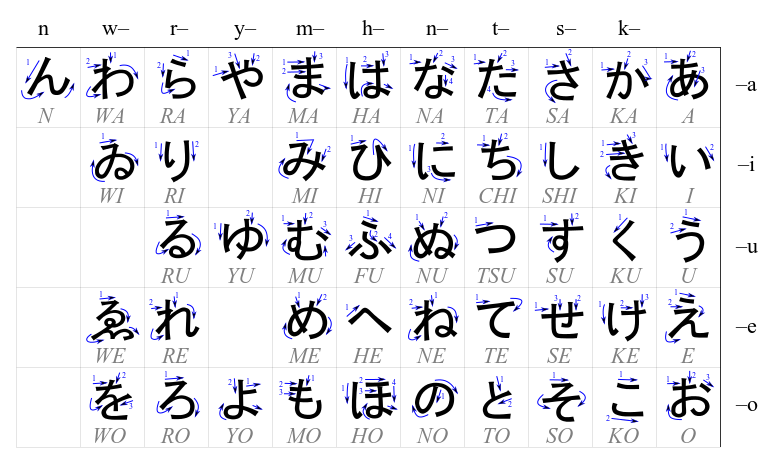
\includegraphics[scale=.2]{material/05Table_hiragana}
	\caption{Hiragana mit lat. Umschrift}
	\label{Hiragana}
\end{figure}
\end{minipage}

\end{frame}


%%%%%%%%%%%%%%%%%%%%%%%%%%%%%%%%%%
\begin{frame}
\frametitle{Phonographische Schrifttypen: Syllabisch}

%\begin{minipage}{.59\textwidth}
\begin{itemize}
	\item Korrespondenz zwischen \textbf{graphischem Zeichen} und \textbf{Silbe}
	\item Japanisch, Koreanisch, \dots
	
	%\ex. Japanisch: [Japanisch Package] für die Silbe \textipa{[ka]} (in der Silbenschrift Hiragana)

\end{itemize}
%\end{minipage}\hfill%
%%
%%
%\begin{minipage}{.4\textwidth}
	\begin{figure}
		\centering
		
		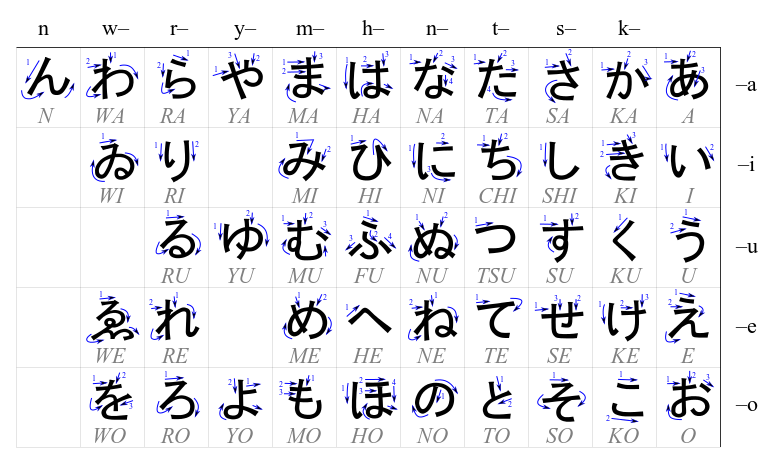
\includegraphics[scale=.25]{material/05Table_hiragana}
		\caption{Hiragana mit lat. Umschrift}
%		\label{Hiragana}
	\end{figure}
%\end{minipage}

\end{frame}


%%%%%%%%%%%%%%%%%%%%%%%%%%%%%%%%%%
\begin{frame}
\frametitle{Phonographische Schrifttypen: Alphabetisch}


\begin{itemize}

	\item Korrespondenz zwischen \textbf{graphischem Zeichen} (Buchstaben) und \textbf{Lauten}
	\item Deutsch, Russisch, Arabisch, \dots
	
	\ea Deutsch: \ab{t} für Laut \textipa{[t]}
	\z 
	
	\pause 
	
	\begin{itemize}
		\item \textbf{Konsonant-Vokal-Schrift:} \\
		enthält Grapheme für Konsonanten und Vokale
		\item Deutsch, Russisch, \dots
		
		\item \textbf{Konsonantenschrift:}\\
		enthält Grapheme (fast) nur für Konsonanten \citep[vgl.][358]{Glueck16b} 
		\item nordwestsemitische Schriftarten, Arabisch, Hebräisch, \dots
	\end{itemize}
	
	\end{itemize}

\end{frame}


%%%%%%%%%%%%%%%%%%%%%%%%%%%%%%%%%%
%%%%%%%%%%%%%%%%%%%%%%%%%%%%%%%%%%
\subsubsection{Logographische Schrifttypen}
%\iftoggle{sectoc}{
%	\frame{
%		\begin{multicols}{2}
%			\frametitle{~}
%			\tableofcontents[currentsection]
%		\end{multicols}
%	}
%}
%%%%%%%%%%%%%%%%%%%%%%%%%%%%%%%%%%

\begin{frame}
\frametitle{Logographische Schrifttypen}

\begin{itemize}
	\item Grundformen sind primär auf \textbf{bedeutungstragende} Elemente (\zB Wörter oder Morpheme) im Sprachsystem bezogen \citep[vgl.][76--77]{Duerscheid04a}. 
	
	\item Chinesisch, Teile der ägyptischen Hieroglyphen
\end{itemize}
		
\begin{minipage}{.28\textwidth}
	\begin{figure}
	\centering
	
\includegraphics[scale=.45]{material/Chinesemountain-Lee-Sau-Dan}
	\caption[chinese]{Chinesisches Zeichen für `Berg'}\label{ChinBerg}
	\end{figure}
\end{minipage}\hfill%
%%
\begin{minipage}{.68\textwidth}
	\begin{figure}
	\centering
	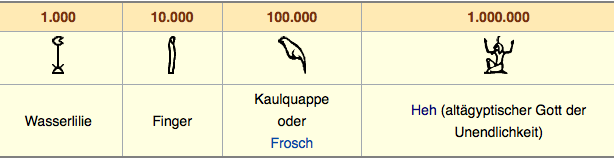
\includegraphics[scale=.37]{material/04Hieroglyphenzahlen}
	\caption[Hiero]{Hieroglyphenzahlen}\label{Hieroglyphen}
	\end{figure}
\end{minipage}
		
\end{frame}


%%%%%%%%%%%%%%%%%%%%%%%%%%%%%%%%%%
%%%%%%%%%%%%%%%%%%%%%%%%%%%%%%%%%%
\subsubsection{Fazit: Schrifttypen \& -systeme}
%\iftoggle{sectoc}{
%	\frame{
%		\begin{multicols}{2}
%			\frametitle{~}
%			\tableofcontents[currentsection]
%		\end{multicols}
%	}
%}
%%%%%%%%%%%%%%%%%%%%%%%%%%%%%%%%%%

\begin{frame}
\frametitle{Fazit: Schrifttypen \& -systeme}

\begin{itemize}
	\item Vorteil von \textbf{phonographischen} Schriftsystemen:
	
	\begin{itemize}
		\item große Menge von Wörtern mit \textbf{eher kleinem Inventar von Zeichen} (20--30) darstellbar
	\end{itemize}
	
	\item \textbf{Logographische Schrifttypen} benötigen sehr viele Zeichen.
	
	\begin{itemize}
		\item Das chinesische Schriftsystem besteht aus ungefähr 87\,000 Zeichen,\\
                  von denen zwischen 3\,000 und 5\,000 für den Alltag benötigt werden.
	\end{itemize}
	
\pause 	

	\item Vorteil von \textbf{logographischen} Schriftsystemen:
	\begin{itemize}
		\item Sie können auch von Lesern anderer Dialekte \textbf{relativ leicht dekodiert} werden.
	\end{itemize}	
\end{itemize}
\end{frame}


%%%%%%%%%%%%%%%%%%%%%%%%%%%%%%%%%%%%
%\begin{frame}
%\frametitle{Übersicht der Schrifttypen \& -systeme}
%
%
%\begin{figure}
%\centering
%\scalebox{.85}{
%	\begin{forest}
%		MyP edges
%		[\textbf{\alertred{Schrifttypen}}
%			[\textbf{logographischer} \\ Schrifttyp
%			[Chinesisch \\ Hieroglyphen, tier=word]
%			]
%			[\textbf{phonographischer} \\ Schrifttyp
%				[\textbf{alphabetischer} \\ Schrifttyp
%					[\textbf{Konsonant-Vokal-}\\Schriften
%						[Latein \\ Griechisch \\ Russisch, tier=word]
%					]
%					[\textbf{Konsonanten-}\\schriften
%						[Hebräisch \\ Arabisch, tier=word]
%					]
%				]
%				[\textbf{syllabischer} \\ Schrifttyp
%					[Japanisch \\ Koreanisch, tier=word, name=anchor] {
%					\node [right=of anchor]{\textbf{\alertred{Schriftsysteme}}};
%					}
%				]
%			]
%		]
%	\end{forest}
%}
%\end{figure}
%
%\end{frame}
%
%
%%%%%%%%%%%%%%%%%%%%%%%%%%%%%%%%%%
%%%%%%%%%%%%%%%%%%%%%%%%%%%%%%%%%%
\subsubsection{Tiefe \vs flache Systeme}
%\iftoggle{sectoc}{
%	\frame{
%		\begin{multicols}{2}
%			\frametitle{~}
%			\tableofcontents[currentsection]
%		\end{multicols}
%	}
%}
%%%%%%%%%%%%%%%%%%%%%%%%%%%%%%%%%%

\begin{frame}
\frametitle{Tiefe vs.\ flache Systeme}

\begin{itemize}
	\item trotz phonographischer/""alphabetischer Schriftsysteme \ras\\
              sehr verschiedene Schreibung in den unterschiedlichen Sprachen

	\item unterschiedliche \textbf{graphematische (/orthographische) Prinzipien},\\
          die den unterschiedlichen Schreibungen zugrunde liegen

	\item Selten 1-zu-1-Korrespondenz zwischen Phonemen und Graphemen
	
	\begin{itemize}
		\item \textbf{tiefes System}\\ 
		\vs
		\item \textbf{flaches System}
	\end{itemize}
\end{itemize}
\end{frame}


%%%%%%%%%%%%%%%%%%%%%%%%%%%%%%%%%%
\begin{frame}
\frametitle{Tiefe vs.\ flache Systeme}
\begin{itemize}
	
	\item \textbf{flaches System:}

	\begin{itemize}
		
		\item sehr gute 1-zu-1-Abbildung von Phonemen und Graphemen
		
		\item \textbf{Türkisch}
		
		\begin{itemize}
			
			\item 1928: Ersetzung der arabischen Schrift durch die lateinische Schrift
			
			\item besonders gute Phonem-Graphem-Abbildung
		\end{itemize}
	\end{itemize}

\pause 

	\item \textbf{tiefes System:}

\begin{itemize}

	\item Abbildung von Phonemen auf Graphemen, aber mit Einschränkung

	\item \textbf{Englisch} oder \textbf{Französisch}
	
	\begin{itemize}
		\item nicht häufig \textbf{reformiert} \ras starke Abweichung von Aussprache und Schriftform

		\item Englisch: \textbf{altes} und \textbf{gewachsenes} System mit sehr verschiedenen \textbf{Dialekten} in unterschiedlichen Ländern

		\item schriftliche Verständigung zwischen den Varietäten ist nur gewährleistet,\\
		wenn die Phonem-Graphem-Korrespondenz nicht streng durchgezogen wird.
	\end{itemize}
\end{itemize}
\end{itemize}

\end{frame}


%%%%%%%%%%%%%%%%%%%%%%%%%%%%%%%%%%
\begin{frame}
\frametitle{Tiefe vs.\ flache Systeme}


	\ea Türkisch: \\
	\ab{dükkan} für \textipa{[dYkkan]}
	
	\ex Spanisch: \\
	\ab{negocio} für \textipa{[negoTio]}
	
	\ex Englisch: \\
	\ab{business} für \textipa{[bIzn@z]}
	
	\ex Französisch: \\
	\ab{boutique} für \textipa{[butik]}
	\z 
	
\pause	
	
	\ea English: \ab{gh o ti} für \ab{fish} 

\pause  
	
	(\ab{gh} wie in \ab{enou\alertred{gh}}, \ab{o} wie in \ab{w\alertred{o}men}, \ab{ti} wie in \ab{na\alertred{ti}on}
	\z 

\end{frame}


%%%%%%%%%%%%%%%%%%%%%%%%%%%%%%%%%%
\begin{frame}
\frametitle{Tiefe vs.\ flache Systeme}


\begin{figure}
\centering
	
\includegraphics[scale=.3]{material/04GraphEnglischPGK}
	\caption{Englisch und PGK}\label{grammarlycard}
%{https://www.facebook.com/grammarly/photos/a.158139670871698.33824.139729956046003/942699349082389/; Autor: Grammarly; Stand: 05.12.16}
\end{figure}

\end{frame}


%%%%%%%%%%%%%%%%%%%%%%%%%%%%%%%%%%
%%%%%%%%%%%%%%%%%%%%%%%%%%%%%%%%%%
\subsection{Graphematische Prinzipien}

%% MyP: Contents
\iftoggle{sectoc}{
	\frame{
		%\begin{multicols}{2}
		\frametitle{~}
		\tableofcontents[currentsubsection, subsubsectionstyle=hide]
		%\end{multicols}
	}
}

%% StM: Contents
\iftoggle{gliederung}{
	
	\outline{
		\begin{itemize}
			
			\item Einführung
			\item Graph, Graphem, Allograph
			\item Graphematik \vs Orthographie
			\item Schrifttypen \& -systeme
			%%Phonographische Schrifttypen
			%%Logographische Schrifttypen
			%%Fazit: Schrifttypen & -systeme
			%%Tiefe vs. flache Systeme
			\item \blaubf{Graphematische Prinzipien}
			%%Phonographisches Prinzip
			%%Silbisches Prinzip
			%%Morphologisches Prinzip
			%%Differenzierung homophoner Formen
			%%Etymologische Schreibung
			%%Ästhetische Schreibung
			%%Syntaktische Schreibung
			\item Hausaufgabe
			
		\end{itemize}
	}
}


%%%%%%%%%%%%%%%%%%%%%%%%%%%%%%%%%%
\begin{frame}
\frametitle{Graphematische Prinzipien/Tendenzen}

\begin{itemize}
	\item \textbf{Schrifttyp} bedingt das graphematische System.
	\item Daraus ergibt sich die \textbf{Gewichtung} (oder Vorhandensein) weiterer
Prinzipien:

	\begin{itemize}
		\item Deutsch: alphabetischer Schrifttyp \ras Abbildung von Phonemen mit Graphemen

		\item Abbildung von Phonemen auf Grapheme $=$ \\
		\textbf{Phonem-Graphem-Korrespondenz} (PGK)
		
		\item Weitere Prinzipien:
		
		\begin{itemize}
			\item \textbf{Wortebene}:\\
			regelhafte Markierung von Silben, Morphemen und Bedeutungseinheiten, \dots

			\item \textbf{Satzebene}: \\
			regelhafte Groß- und Kleinschreibung, Zusammen- und Getrenntschreibung, \dots
		\end{itemize}
	
	\end{itemize}

\end{itemize}
\end{frame}


%%%%%%%%%%%%%%%%%%%%%%%%%%%%%%%%%%
\begin{frame}
\frametitle{Graphematische Prinzipien/Tendenzen}

\begin{itemize}
	\item Das graphematische System des Deutschen wird von diesen
	\textbf{meist regelhaften Prinzipien bestimmt} und dementsprechend
	(anschließend) auch \textbf{normiert}, sodass es nur eine einzige
	mögliche (normierte) Schreibung für ein Wort gibt.
	
	\begin{itemize}
		\item Erkundung und Erklärung von Regelmäßigkeiten des Systems \\
		\ras \textbf{graphematische Herangehensweise}
		
		\item Anwendung der Regelmäßigkeiten mit einem präskriptiven,
		normativen Charakter \\
		\ras \textbf{orthographische Herangehensweise}
	\end{itemize}
\end{itemize}

\end{frame}


%%%%%%%%%%%%%%%%%%%%%%%%%%%%%%%%%%
\begin{frame}
\frametitle{Graphematische Prinzipien/Tendenzen}

\begin{itemize}
	\item Graphematische/Orthographische \gqq{Prinzipien/Tendenzen}:
	
	\begin{itemize}
		\item Phonographisches Prinzip (nach Phonem-Graphem-Korrespondenzen)

		\item Silbisches Prinzip

		\item Morphologisches Prinzip (auch Prinzip der Morphemkonstanz)

		\item Differenzierung homophoner Formen

		\item Etymologische Schreibung

		\item Ästhetische Schreibung 

		\item Syntaktische Schreibung 
	\end{itemize}

\item  Es handelt sich eher um \textbf{Tendenzen} (weniger um Prinzipien), weil sie nicht immer vollkommen \textbf{regelhaft} sind.

\end{itemize}


\end{frame}


%%%%%%%%%%%%%%%%%%%%%%%%%%%%%%%%%%
%%%%%%%%%%%%%%%%%%%%%%%%%%%%%%%%%%
\subsubsection{Phonographisches Prinzip}
%\iftoggle{sectoc}{
%	\frame{
%		\begin{multicols}{2}
%			\frametitle{~}
%			\tableofcontents[currentsection]
%		\end{multicols}
%	}
%}
%%%%%%%%%%%%%%%%%%%%%%%%%%%%%%%%%%

\begin{frame}
\frametitle{Phonographisches Prinzip}

\begin{itemize}
	\item Phoneme werden mit Graphemen wiedergegeben.
	\item \textbf{Phonem-Graphem-Korrespondenzen} (auch PGK-Regeln)

\pause	

	\item Abbildung von \textbf{Lauten} (Phonen) in Form von Buchstaben (Phon--Graphem)\\ 
	\vs
	\item Abbildung von \textbf{abstrakten, regulären Lautmengen} in
Form von Buchstaben (Phonem--Graphem)

\end{itemize}

\end{frame}


%%%%%%%%%%%%%%%%%%%%%%%%%%%%%%%%%%
\begin{frame}
\frametitle{Phonographisches Prinzip}

\begin{itemize}
	
	\item \textbf{Pro}: Phon $\leftrightarrow$ Graphem

	\begin{itemize}
		\item sehr genaue Abbildung
		\item einfach für den Leser
	\end{itemize}

\pause 
	
	\item \textbf{Contra}: Phon $\leftrightarrow$ Graphem
	
	\begin{itemize}
		\item größeres Inventar an Buchstaben nötig
		
		\ea Unterschiedliche Buchstaben(-kombinationen) für \ab{ch}\\
		\zB in \ab{i\alertred{ch}} und \ab{Bu\alertred{ch}}
		\z 

\pause 		

		\item Variabilität der Aussprache in einem Dialekt und in unterschiedlichen Dialekten
		
		\ea Unterschiedliche Schreibung von \ab{Sport},\\
		\zB \ab{Spo\alertred{R}t}, \ab{Spo\alertred{r}t}, \ab{Spo\alertred{a}t}, \ab{Spo\alertred{ch}t}
		\z 

\pause 
		
		\item \gqq{Verwandtschaft} zwischen Wortformen nicht mehr erkennbar
		
		\ea Unterschiedliche Schreibung von \ab{r}\\
		\zB in \ab{hö\alertred{a}t} \vs \ab{hö\alertred{r}en}
		\z 
	\end{itemize}
\end{itemize}

\end{frame}


%%%%%%%%%%%%%%%%%%%%%%%%%%%%%%%%%%
\begin{frame}
\frametitle{Phonographisches Prinzip}

\begin{itemize}
	\item \textbf{Pro} Phonem $\leftrightarrow$ Graphem
	
	\begin{itemize}
		\item einheitliche Wiedergabe von komplementärer, freier und regionaler \textbf{Allophonie}

		\item \textbf{Definition von Graphem} als kleinste bedeutungsunterscheidende Einheit eines Schriftsystems (parallel zu Phonem)
	\end{itemize}

\pause 
	
	\item \textbf{Contra} Phonem $\leftrightarrow$ Graphem
	
	\begin{itemize}
		\item etwas komplizierter \textbf{für den Leser}
		
		\ea Wann wird ein \ab{ch} wie in \ab{i\alertred{ch}} oder wie in \ab{Bu\alertred{ch}} ausgesprochen?
		\z 
		
		\item ABER: Dafür \textbf{reduziert} sich der \textbf{Lernaufwand} bzgl.\ der Menge von zu lernenden Buchstaben.	
	\end{itemize}
\end{itemize}

\end{frame}


%%%%%%%%%%%%%%%%%%%%%%%%%%%%%%%%%%
\begin{frame}
\frametitle{PGK: Konsonanten}

\begin{table}
\centering
\scalebox{0.8}{
\begin{tabular}{l l l | l l l}
\textbf{Phonem} & \textbf{einige mögliche} & \textbf{Graphem} & \textbf{Phonem} & \textbf{einige mögliche } & \textbf{Graphem} \\
& \textbf{Allophone} & & & \textbf{Allophone} & \\ 
\textipa{/p/} & \textipa{[p], [p\super h]} & \ab{p} & \textipa{/\c{c}/} & \textipa{[\c{c}], [x]} & \ab{ch} \\
\textipa{/t/} & \textipa{[t], [t\super h]} & \ab{t} & \textipa{/v/} & \textipa{[v]} & \ab{w} \\
\textipa{/k/} & \textipa{[k], [k\super h]} & \ab{k} & \textipa{/j/} & \textipa{[j]} & \ab{j} \\
\textipa{/b/} & \textipa{[b], [p]} & \ab{b} & \textipa{/h/} & \textipa{[h]} & \ab{h} \\
\textipa{/d/} & \textipa{[d], [t]} & \ab{d} & \textipa{/m/} & \textipa{[m]} & \ab{m} \\
\textipa{/g/} & \textipa{[g], [k]} & \ab{g} & \textipa{/n/} & \textipa{[n]} & \ab{n} \\
\textipa{/k/+/v/} & [\textsubplus{k}]\textipa{[v]} & \ab{qu} & \textipa{/l/} & \textipa{[l]} & \ab{l} \\
\textipa{/f/} & \textipa{[f]} & \ab{f} & /\textscr{}/ & [\textscr{}], \textipa{[K], [r], [5]} & \ab{r} \\
\textipa{/s/} & \textipa{[s]} & \ab{ß} & \textipa{/\t{pf}/} & \textipa{[\t{pf}]} & \ab{pf} \\
\textipa{/s/} & \textipa{[s]} & \ab{s} &   &   &   \\
\textipa{/z/} & \textipa{[z], [s]} & \ab{s} & \textipa{/\t{ts}/} & \textipa{[\t{ts}]} & \ab{z} \\
\textipa{/S/} & \textipa{[S]} & \ab{sch} & \textipa{/\t{tS}/} & \textipa{[\t{tS}]} & \ab{tsch} \\
	
\end{tabular} 
}
%\caption{Phonem-Graphem-Korrespondenzen für Konsonanten}
\end{table}

\pause 

\ea \textipa{/s/}, \textipa{[s]}, \ab{\alertred{ß}} (zwischensilbisch nach XX im Nukleus): au\ab{\alertred{ß}}er, Mu\ab{\alertred{ß}}e

\ex \textipa{/s/}, \textipa{[s]}, \ab{\alertred{s}} (im Auslaut): da\ab{\alertred{s}}, e\ab{\alertred{s}}

\ex \textipa{/z/}, \textipa{[z], [s]}, \ab{\alertred{s}}: \ab{\alertred{s}}ieh\ab{\alertred{s}}t  
\z 


\end{frame}


%%%%%%%%%%%%%%%%%%%%%%%%%%%%%%%%%%%
\begin{frame}
\frametitle{PGK: Vokale}


\begin{table}
\centering
%\scalebox{0.8}{
\begin{tabular}{l l | l l}
	\textbf{Vokalphonem} & \textbf{Graphem} & \textbf{Vokalphonem} & \textbf{Graphem} \\
	\textbf{(lang und gespannt)} & & \textbf{(kurz und ungespannt)} & \\
	\textipa{/i:/} & \ab{ie} & \textipa{/I/} & \ab{i} \\
	\textipa{/y:/} & \ab{ü} & \textipa{/Y/} & \ab{ü} \\
	\textipa{/e:/} & \ab{e} & & \\
	\textipa{/E:/} & \ab{ä} & \textipa {/E/} & \ab{e} \\
	& & \textipa{/@/} & \ab{e} \\
	\textipa{/\o:/} & \ab{ö} & 	\textipa{/\oe/} & \ab{ö} \\
	\textipa{/A:/} & \ab{a} & \textipa{/a/} & \ab{a} \\
	\textipa{/o:/} & \ab{o} & \textipa{/O/} & \ab{o} \\ 
	\textipa{/u:/} & \ab{u} & \textipa{/U/} & \ab{u} \\
\end{tabular}
%}
%\caption{Phonem-Graphem-Korrespondenzen für Vokale}
\end{table}

\end{frame}


%%%%%%%%%%%%%%%%%%%%%%%%%%%%%%%%%%
\begin{frame}
\frametitle{PGK: Diphthonge}

\begin{table}
	\centering
%	\scalebox{0.8}{
	\begin{tabular}{l l}
		\textbf{Diphthong} & \textbf{Digraph} \\
		\textipa{/\t{aI}/} & \ab{ei} \\
		\textipa{/\t{aU}/} & \ab{au} \\
		\textipa{/\t{O}I/} & \ab{eu} \\	
	\end{tabular}		
%	}
%\caption{Phonem-Graphem-Korrespondenzen für Diphthonge}
\end{table}

\begin{description}
	\item[Digraph] Graphem aus zwei Buchstaben 
	
	\item[Trigraph] Graphem aus drei Buchstaben
\end{description}

\end{frame}


%%%%%%%%%%%%%%%%%%%%%%%%%%%%%%%%%%
\begin{frame}
\frametitle{Übung}

\begin{itemize}
	\item Geben Sie 10 Wörter an, die phonographisch geschrieben werden.
	\item Wie würden Sie die folgenden Wörter phonographisch schreiben?

	\ea\label{ex:04aphilo}
		\ea Philosophie
		\ex Balkon
		\ex Creme
		\ex Mutter
		\ex Streithahn
		\z
	\z
	
\end{itemize}
	
\end{frame}


%%%%%%%%%%%%%%%%%%%%%%%%%%%%%%%%%
%%%%%%%%%%%%%%%%%%%%%%%%%%%%%%%%%
\iftoggle{ue-loesung}{
	%%%%%%%%%%%%%%%%%%%%%%%%%%%%%%%%%%
%% UE 1 - 04a Graphematik
%%%%%%%%%%%%%%%%%%%%%%%%%%%%%%%%%%

\begin{frame}
\frametitle{Übung -- Lösung}

\begin{itemize}
	\item Geben Sie 10 Wörter an, die phonographisch geschrieben werden.
	
		\begin{description}
			\item[\alertred{\textbf{Beispiele:}}] \alertred{Beurteilung, schön, Gabel, suchen, Macht, Lager, kurz, niesen, Zopf, Gewerkschaft}
		\end{description}
	
	\item Wie würden Sie die folgenden Wörter phonographisch schreiben?
		
	\begin{exe}
		\exr{ex:04aphilo}
	\settowidth\jamwidth{XXXXXXXXXXXXXXXXXXXXXXXXXXXXX}
		\begin{xlist}
			\ex Philosophie \loesung{2}{\ab{filosofie}}
			\ex Balkon \loesung{3}{\ab{balkong}}
			\ex Creme \loesung{4}{\ab{krem} oder \ab{kreme}}
			\ex Mutter \loesung{5}{\ab{muter}}
			\ex Streithahn \loesung{6}{\ab{schtreithan}}
		\end{xlist}
	\end{exe}
		

\end{itemize}

\end{frame}


}

%%%%%%%%%%%%%%%%%%%%%%%%%%%%%%%%%%
\begin{frame}
\frametitle{Übung}

\begin{itemize}	
	\item Versuchen Sie, graphematische Regularitäten und Prinzipien zu finden, die die Unterscheidung "`lang \vs kurz"' bei Vokalen anzeigen. Gibt es Ausnahmen?
	
	\ea\label{ex:04amutter}
	
	\begin{multicols}{2}
		\ea Mutter
		\ex Mehl
		\ex See
		\ex Nase
		\ex dehnen
		\ex gehen
		\ex Bier
		\ex Moor
		\ex an
		\ex zum
		\ex Mann
		\ex man
		\ex Herbst
		\ex Laub
		\ex sehr
		\ex Bohrer
		\z
	\end{multicols}
	
	\z
	
\end{itemize}

\end{frame}


%%%%%%%%%%%%%%%%%%%%%%%%%%%%%%%%%%
%%%%%%%%%%%%%%%%%%%%%%%%%%%%%%%%%%
\iftoggle{ue-loesung}{
	%%%%%%%%%%%%%%%%%%%%%%%%%%%%%%%%%%
%% UE 2 - 04a Graphematik
%%%%%%%%%%%%%%%%%%%%%%%%%%%%%%%%%%

\begin{frame}
\frametitle{Übung -- Lösung}

\begin{itemize}	
	\item Versuchen Sie, graphematische Regularitäten und Prinzipien zu finden, die die Unterscheidung lang \vs kurz bei Vokalen anzeigen. Gibt es Ausnahmen?
	
	\ea\label{ex:mutter}
	
	\begin{multicols}{2}
		\ea Mutter
		\ex Mehl
		\ex See
		\ex Nase
		\ex dehnen
		\ex gehen
		\ex Bier
		\ex Moor
		\ex an
		\ex zum
		\ex Mann
		\ex man
		\ex Herbst
		\ex Laub
		\ex sehr
		\ex Bohrer
		\z
	\end{multicols}
	
	\z
	
	
	
\end{itemize}

\end{frame}


}

%%%%%%%%%%%%%%%%%%%%%%%%%%%%%%%%%%
%%%%%%%%%%%%%%%%%%%%%%%%%%%%%%%%%%
\subsubsection{Silbisches Prinzip}
%\frame{
%\frametitle{~}
%	\tableofcontents[currentsection]
%}


%%%%%%%%%%%%%%%%%%%%%%%%%%%%%%%%%%
\begin{frame}
\frametitle{Silbisches Prinzip}

\begin{itemize}
	\item auch durch die Lautstruktur zu begründen, aber nicht reine Phonem-Graphem-Beziehungen \ras Bezug auf Vokalqualität/-quantität
	
	\item In der Graphematik wird (analog zur Silbe in der Phonologie) eine Silbe angenommen \citep[vgl.][]{Fuhrhop08a}:
	
	\begin{itemize}
		\item[]
		\item \textbf{Anfangsrand}: Konsonant(en),\\
		leerer Anfangsrand: \textbf{nackte} Silbe\\
		besetzter Anfangsrand: \textbf{bedeckte} Silbe
		\item[]
		\item \textbf{Silbenkern}: Vokal oder Diphthong
		\item[]
		\item \textbf{Endrand}: Konsonant(en)\\
		leerer Endrand: \textbf{offene} Silbe\\
		besetzter Endrand: \textbf{geschlossene} Silbe
	\end{itemize}
\end{itemize}

\end{frame}


%%%%%%%%%%%%%%%%%%%%%%%%%%%%%%%%%%
\begin{frame}
\frametitle{Silbisches Prinzip: (Un-)Gespanntheit}

\begin{itemize}
	\item Vokalqualität (\dash Gespanntheit) und -quantität (\dash Länge) wird phonographisch nicht eindeutig abgebildet (s.\ PGK für Vokale), aber es gibt \textbf{Tendenzen auf Silbenebene}.
	\item[]
	\item für \textbf{morphologisch einfache Wörter} 
	
	\begin{itemize}
		\item offene Silbe \ras \textbf{gespannter} Vokal: 
		
		\ea \ab{Kl\alertred{o}}, \ab{s\alertred{o}} (weitere Markierung: \ab{Se\alertred{e}}, \ab{Re\alertred{h}})
		\z
		
		\item geschlossene Silbe mit komplexem Endrand \ras \textbf{ungespannter} Vokal: 
		
		\ea
		\ab{Stru\alertred{mpf}}, \ab{Bi\alertred{ld}}
		\z
		
		\item wenige \textbf{Ausnahmen} \citep[vgl.][15]{Fuhrhop09a}: 
		
		\ea
		\ab{Mo\alertred{nd}}, \ab{Ke\alertred{ks}}, \ab{O\alertred{bst}}
		\z
		
	\end{itemize}
\end{itemize}
\end{frame}


%%%%%%%%%%%%%%%%%%%%%%%%%%%%%%%%%%
\begin{frame}
\frametitle{Silbisches Prinzip: (Un-)Gespanntheit}

\begin{itemize}
	\item für \textbf{morphologisch einfache Wörter}
	
	\begin{itemize}
		\item geschlossene Silbe mit einfachem Endrand \ras \textbf{gespannter} oder \textbf{ungespannter} Vokal möglich:
		
		\ea \ab{B\alertred{ee}t} -- \ab{B\alertred{e}tt}, \ab{B\alertred{a}hn} -- \ab{B\alertred{a}nn}
		\z

\pause 
		
		\item \textbf{zusätzliche Markierungen} möglich, aber nicht immer markiert: 
		
		\ea 
			\ea ungespannt/kurz: \ab{a\alertred{n}}, \ab{bi\alertred{s}}
		
			\ex gespannt/lang: \ab{ro\alertred{t}}, \ab{Hu\alertred{t}}
			\z
		\z 
	\end{itemize}
\end{itemize}

\end{frame}


%%%%%%%%%%%%%%%%%%%%%%%%%%%%%%%%%%
\begin{frame}
\frametitle{Silbisches Prinzip: Markierungen der (Un-)Gespanntheit}

	\begin{itemize} 
		\item Markierung der \textbf{Gespanntheit} durch \textbf{Verdoppelung des Vokals} \ab{aa}, \ab{ee}, \ab{oo} oder \ab{\textbf{ie}} 
		
		\ea \ab{B\alertred{ee}t}, \ab{S\alertred{aa}l}, \ab{B\alertred{oo}t}, \ab{T\alertred{ie}r}, \ab{M\alertred{eh}l}
		\z

		\begin{itemize}
			\item lediglich \ab{ee} findet sich auch in offenen Silben, vermutlich weil \ab{e} sowohl für /\textschwa{}/ als auch für \textipa{/e/} steht.
		
		\ea \ab{S\alertred{ee}}, \ab{Arm\alertred{ee}}, \ab{Klisch\alertred{ee}}, \ab{All\alertred{ee}}%, \ab{\textbf{Orchidee}}
		\z
		\end{itemize}
	
		\item vor \textbf{Sonoranten}: Markierung der \textbf{Gespanntheit} durch ein \ab{\textbf{h}} \textbf{nach dem Vokal} (Dehnungs-h) 
		
		\ea \ab{Me\alertred{h}l}, \ab{Bo\alertred{h}rer}, \ab{Ba\alertred{h}n}
		\z
	\end{itemize}

\end{frame}


%%%%%%%%%%%%%%%%%%%%%%%%%%%%%%%%%%
\begin{frame}
\frametitle{Silbisches Prinzip: Ungespanntheit \& Silbengelenk}

\begin{itemize}
	\item \textbf{Ungespanntheit} wird \ua durch die \textbf{Verdopplung des Folgekonsonanten} (Geminatenschreibung) angezeigt, in zweisilbigen Wörtern sind diese Konsonanten dann \textbf{ambisyllabisch} (\dash Silbengelenk): 


\ea \ab{E\alertred{bb}e}, \ab{A\alertred{ff}e}, \ab{Kla\alertred{dd}e}
\z

	\item Achtung: Im Deutschen markiert die \textbf{Konsonantenverdopplung} primär ein \textbf{Silbengelenk}. Silbenkgelenke kommen \textbf{nach kurzen ungespannten Vokalen} vor.
	
	\item In Fällen wie (\ref{ex:GraphGelenk1}) korreliert die Geminatenschreibung mit dem morphologischen Prinzip, vgl.\ (\ref{ex:GraphGelenk2}).

	\ea 
	\ea\label{ex:GraphGelenk1} \ab{Fa\alertred{ll}}, \ab{Ma\alertred{nn}}
	\ex\label{ex:GraphGelenk2} \ab{Fä\alertred{ll}e}, \ab{Mä\alertred{nn}er}
	\z
	\z 
\end{itemize}
\end{frame}


%%%%%%%%%%%%%%%%%%%%%%%%%%%%%%%%%%
\begin{frame}
\frametitle{Silbisches Prinzip: silbentrennendes \ab{h}}
	
	\begin{itemize}
	\item zwischen zwei \textbf{vokalischen Silbenkernen} zur \textbf{Markierung der Zweisilbigkeit}
	
	
	\eal
	\ex \ab{ge-\alertred{h}en}
	\ex \ab{Ru-\alertred{h}e}
	\ex \ab{Mü-\alertred{h}e}
	\zl

\pause
	
	\item besonders häufig in Verben
	\eal
	\ex \ab{se\alertred{h}en}
	\ex \ab{ste\alertred{h}en}
	\zl
	
\pause
	
	\item nicht nach Diphthongen, außer \ab{ei}
	\eal
	\ex \ab{h\alertblue{au}en}
	\ex \ab{sch\alertblue{au}en}
	\ex \ab{lei\alertred{h}en}
	\ex \ab{verzei\alertred{h}en}
	\ex \ab{schr\alertblue{ei}en}
	\zl

	\end{itemize}

\end{frame}


%%%%%%%%%%%%%%%%%%%%%%%%%%%%%%%%%%
%%%%%%%%%%%%%%%%%%%%%%%%%%%%%%%%%%
\subsubsection{Morphologisches Prinzip}
%\iftoggle{sectoc}{
%	\frame{
%		\begin{multicols}{2}
%			\frametitle{~}
%			\tableofcontents[currentsection]
%		\end{multicols}
%	}
%}
%%%%%%%%%%%%%%%%%%%%%%%%%%%%%%%%%%

\begin{frame}
\frametitle{Morphologisches Prinzip}

\begin{itemize}
	\item auch Prinzip der Morphemkonstanz, Stammschreibungsprinzip, Verwandtschaftsprinzip
	
	\item Wörter oder Wortformen, die in einer \textbf{morphologischen Beziehung} stehen, werden ähnlich oder gleich geschrieben.
	
	\eal
	\ex \ab{\alertred{A}pfel} -- \ab{\alertred{Ä}pfel}, nicht \ab{Epfel}
	\ex \ab{Hun\alertred{d}} -- \ab{Hun\alertred{d}e}, nicht \ab{Hunt}
	\ex \ab{gro\alertred{ß}} -- \ab{grö\alertred{ß}er}, nicht \ab{gros}
	\ex \ab{B\alertred{a}\alertblue{ll}} -- \ab{B\alertred{ä}\alertblue{ll}e}, nicht \ab{Bal} und \ab{Belle}
	\zl

	\item Bei einigen (wenigen) Wörtern sind zwei Schreibungen zugelassen, um die Verwandtschaft zu verschiedenen Derivaten des gleichen Morphems zu kennzeichnen.
	
	\ea 
	\ea \ab{aufw\alertred{ä}ndig} zu \ab{Aufw\alertred{a}nd}
	\ex \ab{aufw\alertred{e}ndig} zu \ab{aufw\alertred{e}nden}
	\z
	\z 
\end{itemize}

\end{frame}


%%%%%%%%%%%%%%%%%%%%%%%%%%%%%%%%%%
%%%%%%%%%%%%%%%%%%%%%%%%%%%%%%%%%%
%\subsubsection{Übung}
%\frame{
%\frametitle{~}
%	\tableofcontents[currentsection]
%}

%%%%%%%%%%%%%%%%%%%%%%%%%%%%%%%%%%
\begin{frame}
\frametitle{Übung}

\begin{itemize}
	\item Warum schreibt man \ab{dehnen} mit \ab{h}, obwohl das erste \ab{e} in einer offenen Silbe steht und daher nach silbischen Prinzipien sowieso lang gesprochen werden müsste?
	\item[]
	\item Warum schreibt man \ab{mann} und \ab{ball}, obwohl nach silbischen Prinzipien die Geminate einen ambisyllabischen Konsonanten anzeigt?
	\item[]
	\item Warum sind die Wörter \ab{(du) ziehst}, \ab{säubern} und \ab{(er) fällt} Beispiele für morphologisches Schreiben?
	\item[]
	\item Wie hätte eine Person, die \ab{Rad} und \ab{König} als Beispiele für das morphologische Prinzip anführt, \gqq{phonographisches Schreiben} verstanden?
\end{itemize}


\end{frame}


%%%%%%%%%%%%%%%%%%%%%%%%%%%%%%%%%%
%%%%%%%%%%%%%%%%%%%%%%%%%%%%%%%%%%
\iftoggle{ue-loesung}{
	%%%%%%%%%%%%%%%%%%%%%%%%%%%%%%%%%%
%% UE 3 - 04a Graphematik
%%%%%%%%%%%%%%%%%%%%%%%%%%%%%%%%%%

\begin{frame}
\frametitle{Übung -- Lösung}

\begin{itemize}
	\item Warum schreibt man \ab{dehnen} mit \ab{h}, obwohl das erste \ab{e} in einer offenen Silbe steht und daher nach silbischen Prinzipien sowieso lang gesprochen werden müsste?
		\item[] \alertred{Morphemkonstanz, da bei Flexionsformen wie \ab{dehnst} geschlossene Silbe}
	\item Warum schreibt man \ab{mann} und \ab{ball}, obwohl nach silbischen Prinzipien die Geminate einen ambisyllabischen Konsonanten anzeigt?
		\item<2->[] \alertred{Morphemkonstanz, da Pluralform Silbengelenk hat}
	\end{itemize}


\end{frame}


%%%%%%%%%%%%%%%%%%%%%%%%%%
\begin{frame}
\frametitle{Übung -- Lösung}

\begin{itemize}
	\item Warum sind die Wörter \ab{(du) ziehst}, \ab{säubern} und \ab{(er) fällt} Beispiele für morphologisches Schreiben?
		\item[] \alertred{\ab{h} im Infinitiv silbentrennend, Singular-Flexionsformen sind jedoch einsilbig;}
		\item<2->[] \alertred{\ab{ä} zeigt die Verwandschaft zu \ab{sauber}: laut PGK schriebe man \textipa{[O\texttoptiebar{}I]} \ab{eu};}
		\item<3->[] \alertred{Konsonantenverdopplung wegen Silbengelenk im Infinitiv, Singular-Flexionsformen sind jedoch einsilbig,\\ \ab{ä} wegen \ab{a} im Infinitiv: \textipa{[E]} wäre nach PGK \ab{e}}
	\item Wie hätte eine Person, die \ab{Rad} und \ab{König} als Beispiele für das morphologische Prinzip anführt, \gqq{phonographisches Schreiben} verstanden?
		\item<4->[] \alertred{Verschriftlichung der \emph{phonetischen} (richtig wäre: \emph{phonologische}) Repräsentation}
\end{itemize}


\end{frame}


}

%%%%%%%%%%%%%%%%%%%%%%%%%%%%%%%%%%
%%%%%%%%%%%%%%%%%%%%%%%%%%%%%%%%%%
\subsubsection{Differenzierung homophoner Formen}
%\frame{
%\frametitle{~}
%	\tableofcontents[currentsection]
%}


%%%%%%%%%%%%%%%%%%%%%%%%%%%%%%%%%%
\begin{frame}
\frametitle{Differenzierung homophoner Formen}

\begin{itemize}
	
	\item auch Homonym(ie)differenzierung, -vermeidung
	
	\item \textbf{Gleichlautende Wörter} mit \textbf{unterschiedlicher Bedeutung} werden orthographisch unterschiedlich repräsentiert.
	
	\ea L\alertred{ei}b -- L\alertred{ai}b; S\alertred{ei}te -- S\alertred{ai}te; L\alertred{ie}d -- (Augen)L\alertred{i}d
	\z
	
	\item Aber:
	
	\ea Kiefer -- Kiefer; Bremse -- Bremse; Ton -- Ton
	\z
	
	\item Möglichkeiten zur Homophonendifferenzierung werden also keineswegs konsequent ausgenutzt.
\end{itemize}

\end{frame}


%%%%%%%%%%%%%%%%%%%%%%%%%%%%%%%%%%
%%%%%%%%%%%%%%%%%%%%%%%%%%%%%%%%%%
\subsubsection{Etymologische Schreibung}
%\iftoggle{sectoc}{
%	\frame{
%		\begin{multicols}{2}
%			\frametitle{~}
%			\tableofcontents[currentsection]
%		\end{multicols}
%	}
%}
%%%%%%%%%%%%%%%%%%%%%%%%%%%%%%%%%%

\begin{frame}
\frametitle{Etymologische Schreibung}

\begin{itemize}
	\item Die Schreibung \gqq{\textbf{alter}} oder \textbf{entlehnter} Wörter bleibt erhalten,\\
	auch wenn sie nicht den aktuellen Schreibprinzipien entspricht.
	
	\eal
		\ex \ab{wa\alertred{nn}} statt \ab{wan} (wegen mhd. \ab{wanne})
		%% Hier ist kein Silbengelenk möglich!
		
		\ex \ab{\alertred{C}rem\alertred{e}} statt \ab{Krem}
		
		\ex \ab{Restaurant} statt \ab{Restorong}
		
		\ex \ab{Ort\alertred{h}ogra\alertred{ph}ie} oder \ab{Ort\alertred{h}ografie} statt \ab{Ortografie}
	\zl

\end{itemize}

\end{frame}


%%%%%%%%%%%%%%%%%%%%%%%%%%%%%%%%%%
%%%%%%%%%%%%%%%%%%%%%%%%%%%%%%%%%%
\subsubsection{Ästhetische Schreibung}
%\iftoggle{sectoc}{
%	\frame{
%		\begin{multicols}{2}
%			\frametitle{~}
%			\tableofcontents[currentsection]
%		\end{multicols}
%	}
%}
%%%%%%%%%%%%%%%%%%%%%%%%%%%%%%%%%%

\begin{frame}
\frametitle{Ästhetische Schreibung}

\begin{itemize}
	\item \textbf{Schreibsilben} sollten nicht zu lang und nicht zu kurz sein.
	
	\eal
	\ex \ab{\alertred{S}piel} statt \ab{Schpiel}
	\ex \ab{Schw\alertred{a}n} statt \ab{Schw\alertred{ah}n}
	\zl

\pause 
	
	\item \textbf{Verbot von Doppelschreibungen} von einigen Vokalgraphemen (\ab{i} und \ab{u} sowie Umlaute) -- teilweise bedingt durch \textbf{Verwechslungsgefahr}
	
	\ea
	\ab{ii} wie \ab{ü}; \ab{uu} wie \ab{w}
	\z
	
\pause 
		
	\item Verbot von \textbf{Doppelschreibung von Mehrgraphemen} wie
	
	\eal
		\ex \ab{ng} in \ab{Bearbeitu\textcolor{red}{ngng}en}
		\ex \ab{ch} in \ab{Bü\textcolor{red}{chch}er} 
		\ex \ab{sch} in \ab{graphi\textcolor{red}{schsch}e}
	\zl
	
\end{itemize}

\end{frame}


%%%%%%%%%%%%%%%%%%%%%%%%%%%%%%%%%%
%%%%%%%%%%%%%%%%%%%%%%%%%%%%%%%%%%
\subsubsection{Syntaktisches Prinzip}
%\iftoggle{sectoc}{
%	\frame{
%		\begin{multicols}{2}
%			\frametitle{~}
%			\tableofcontents[currentsection]
%		\end{multicols}
%	}
%}
%%%%%%%%%%%%%%%%%%%%%%%%%%%%%%%%%%

\begin{frame}
\frametitle{Syntaktisches Prinzip}

\begin{itemize}
	\item \textbf{Großschreibung für Substantive} und Substantivierungen von Adjektiven, Verben, Adverbien, Partikeln, usw. 

	\ea das \alertred{J}a, das \alertred{G}estern, das \alertred{I}ch
	\z 
	
	\item Großschreibung von \textbf{Satzanfängen} und in \textbf{Anreden}
	
	\ea \alertred{S}ie, \alertred{I}hr
	\z 

	
	\item Die Großschreibung von Substantiven gibt es nur in der deutschen und luxemburgischen Schreibung.\\
	Während der Rechtschreibreform hat man diskutiert, diese abzuschaffen.\\
	Was denken Sie: Was spräche dafür, was dagegen?

\pause 
	
	\ea Berliner Berliner berlinern berlinernd berlinisches Berlinisch.
	\z 
\end{itemize}

\end{frame}




%%%%%%%%%%%%%%%%%%%%%%%%%%%%%%%%%%
%%%%%%%%%%%%%%%%%%%%%%%%%%%%%%%%%%
%\subsection{Übungen}
%\iftoggle{sectoc}{
%	\frame{
%		\begin{multicols}{2}
%			\frametitle{~}
%			\tableofcontents[currentsection]
%		\end{multicols}
%	}
%}


%%%%%%%%%%%%%%%%%%%%%%%%%%%%%%%%%%
\begin{frame}
\frametitle{Übung}

\begin{itemize}
	\item Welche graphematischen Prinzipien (abgesehen von der phonographischen Schreibung) erklären die Schreibung der folgenden Wörter?
	
	  \ea\label{ex:04azimmer}
	  \begin{multicols}{3}
          \ea \ab{Zimmer}
          \ex \ab{Waise}
          \ex \ab{Wehen}
          \ex \ab{Ruhm}
          \ex \ab{Spaß}
          \ex \ab{Allee}
%          \ex \ab{Gras}
          \z
        \end{multicols}
      \z

	\item Welche graphematische Funktion erfüllt das \ab{h} in den folgenden Wörtern?
	
	  \ea\label{ex:04anacht}
	  \begin{multicols}{4}
          \ea \ab{Nacht}
          \ex \ab{Hilfe}
          \ex \ab{sehen}
          \ex \ab{Mehl}
          \z
        \end{multicols}
      \z
      
	\item Wie würden die folgenden Wörter in phonographischer Schreibung aussehen? Geben Sie zunächst eine phonologische Transkription an (Notation mit /~/) \\
	und schreiben Sie anschließend phonographisch (Notation in \ab{~~}).
	
	\ea\label{ex:04avasenstück}
	\begin{multicols}{3}
		\ea \ab{Handy}
		\ex \ab{Vasenstück}
		\ex \ab{Wannenbad}
		\z
	\end{multicols}
	\z
	
\end{itemize}

\end{frame}

%%%%%%%%%%%%%%%%%%%%%%%%%%%%%%%%
%%%%%%%%%%%%%%%%%%%%%%%%%%%%%%%%%
\iftoggle{ue-loesung}{
%%%%%%%%%%%%%%%%%%%%%%%%%%%%%%%%%%
%% UE 4 - 04a Graphematik
%%%%%%%%%%%%%%%%%%%%%%%%%%%%%%%%%%

\begin{frame}
\frametitle{Übung -- Lösung}

\begin{itemize}
	\item Welche graphematischen Prinzipien (abgesehen von der phonographischen Schreibung) erklären die Schreibung der folgenden Wörter?
	
\begin{exe}
	\exr{ex:04azimmer}
	\settowidth\jamwidth{XXXXXXXXXXXXXXXXXXXXXXXXXXXXXXXXXXX}
	\begin{xlist}
		\ex \ab{Zi\rotul{mm}er} \loesung{1}{silbisches Prinzip: Silbengelenk}
		\ex \ab{W\rotul<2->{a}ise} \loesung{2}{Differenzierung homophoner Formen: zu \ab{weise}}
		\ex \ab{We\rotul<3->{h}en} \loesung{3}{silbisches Prinzip: silbentrennend}
		\ex \ab{Ru\rotul<4->{h}m} \loesung{4}{silbisches Prinzip: Dehnungs-h}
		\ex \ab{\rotul<5->{S}paß} \loesung{5}{ästhetische Schreibung: kein \ab{schp}}
		\ex \ab{A\rotul<6->{llee}} \loesung{6}{silbisches Prinzip: Silbengelenk \ab{ll}, Gespanntheit \ab{ee}}
		%          \ex \ab{Gras}
	\end{xlist}
\end{exe}
	
	\item Welche graphematische Funktion erfüllt das \ab{h} in den folgenden Wörtern?
	
\begin{exe}
	\exr{ex:04anacht}
	\settowidth\jamwidth{XXXXXXXXXXXXXXXXXXXXXXXXXXXXXXXXXXX}
	\begin{xlist}
		\ex \ab{Nacht} \loesung{7}{Teil von Digraph \ab{ch}}
		\ex \ab{Hilfe} \loesung{8}{Phonem-Graphem-Korrespondenz zu \textipa{[h]}}
		\ex \ab{sehen} \loesung{9}{silbentrennend}
		\ex \ab{Mehl} \loesung{10}{Dehnungs-h}
	\end{xlist}
\end{exe}
	
    \end{itemize}

\end{frame}


%%%%%%%%%%%%%%%%%%%%%%%%%%%%%%%%%%%%%%%
\begin{frame}{Übung -- Lösung}

	\begin{itemize}
	\item Wie würden die folgenden Wörter in phonographischer Schreibung aussehen? Geben Sie zunächst eine phonologische Transkription an (Notation mit / ~ /) und schreiben Sie anschließend phonographisch (Notation in \ab{ ~ }).

\begin{exe}
	\exr{ex:04avasenstück}
	\begin{multicols}{3}
	\begin{xlist}
		\ex \ab{Handy} 
		
		\ex \ab{Vasenstück}
		
		\ex \ab{Wannenbad}
		
%		\exi{} 
		\exi{} \only<2->{\alertred{\textipa{/hEn.di/}}}
		\exi{} \only<4->{\alertred{\textipa{/va:.z@n.StYk/}}}
		\exi{} \only<6->{\alertred{\textipa{/va\.n@n.ba:d/}}}

%		\exi{} 
		\exi{} \only<3->{\alertred{\ab{hendi}}}		
		\exi{} \only<5->{\alertred{\ab{wasenschtük}}}		
		\exi{} \only<7->{\alertred{\ab{wanenbad}}}		
	\end{xlist}
	\end{multicols}
\end{exe}
	
	\end{itemize}

\end{frame}


}

%%%%%%%%%%%%%%%%%%%%%%%%%%%%%%%%%%
%%%%%%%%%%%%%%%%%%%%%%%%%%%%%%%%%%
\subsection{Hausaufgabe}
%
%%% MyP: Contents
%\iftoggle{sectoc}{
%	\frame{
%		%\begin{multicols}{2}
%		\frametitle{~}
%		\tableofcontents[currentsubsection, subsubsectionstyle=hide]
%		%\end{multicols}
%	}
%}
%
%%% StM: Contents
%\iftoggle{gliederung}{
%	
%	\outline{
%		\begin{itemize}
%			
%			\item Einführung
%			\item Graph, Graphem, Allograph
%			\item Graphematik \vs Orthographie
%			\item Schrifttypen \& -systeme
%			%%Phonographische Schrifttypen
%			%%Logographische Schrifttypen
%			%%Fazit: Schrifttypen & -systeme
%			%%Tiefe vs. flache Systeme
%			\item Graphematische Prinzipien
%			%%Phonographisches Prinzip
%			%%Silbisches Prinzip
%			%%Morphologisches Prinzip
%			%%Differenzierung homophoner Formen
%			%%Etymologische Schreibung
%			%%Ästhetische Schreibung
%			%%Syntaktische Schreibung
%			\item \blaubf{Hausaufgabe}
%			
%		\end{itemize}
%	}
%}
%
%
%%%%%%%%%%%%%%%%%%%%%%%%%%%%%%%%%%
%%%%%%%%%%%%%%%%%%%%%%%%%%%%%%%%%%

\begin{frame}%[allowframebreaks]
	\frametitle{Hausaufgabe}
	
\begin{itemize}
	
	\item[1.] Kreuzen Sie die korrekten Aussagen an.
	
	\begin{itemize}
		\item[$\circ$] Die Orthographie ist eine linguistische Teildisziplin, die beschreibt wie man schreibt. Die Graphematik ist dagegen keine Teildisziplin der Linguistik, sondern eine \gqq{willkürliche} (normierende) Festlegung.
		\item[$\circ$] Die Graphematik sollte intuitiv beherrschbar sein und das Lesen und Schreiben vereinfachen.
		\item[$\circ$] Das Wort \ab{kalt} ist eine graphematisch \gqq{nackte} Silbe.
		\item[$\circ$] Es gibt im Deutschen eine eindeutige 1-zu-1-Korrespondenz zwischen Buchstaben und Lauten.
		\item[$\circ$] Das Wort \ab{aufwändig} wird aufgrund des morphologischen Prinzips (auch Prinzip der Schemakonstanz, Stammprinzip oder Verwandtschaftsprinzip) mit \ab{ä} geschrieben (vgl. \ab{Aufwand}).
	\end{itemize}
\end{itemize}
\end{frame}


%%%%%%%%%%%%%%%%%%%%%%%%%%%%%%%%%%
\begin{frame}
	\begin{itemize}
		\item[2.] Ordnen Sie die graphematischen Prinzipien links den passenden Beispielen für die entsprechenden Prinzipien rechts zu.
		
		NB: Beachten Sie bitte nicht die Großschreibung.
		
		\vspace{.5cm}
								
		\begin{minipage}{0.45\textwidth}
			\centering
			\begin{tabular}{|l|}
				\hline
				(A) Etymologische Schreibung\\
				\hline
				(B) Homonymievermeidung\\
				\hline
				(C) Morphologisches Prinzip\\
				\hline
				(D) Silbische Prinzip\\
				\hline
				(E) Phonographisches Prinzip\\
				\hline
			\end{tabular}
		\end{minipage}
		\hfill%
		\begin{minipage}{0.45\textwidth}
			\centering
			\begin{tabular}{|p{0.075\textwidth}|l|}
				\hline
				& Bad, Bäder \\
				\hline
				& gehen \\
				\hline
				& Cello, *Tschello \\
				\hline
				& Wahl, Wal\\
				\hline
				& Flasche \\
				\hline
			\end{tabular}
		\end{minipage}

	\end{itemize}
\end{frame}


%%%%%%%%%%%%%%%%%%%%%%%%%%%%%%%%%%
\begin{frame}
	\begin{itemize}
		\item[3.] Betrachten Sie die unten angegebenen Kontexte. Diskutieren Sie kurz anhand dieser Beispiele, ob es sich bei der Groß- und Kleinschreibung des markierten Buchstabens um unterschiedliche Grapheme handeln kann oder nicht.
\eal\label{ex:04aHA3}
			\ex Dieser \underline{W}eg ist sehr steil.
			\ex \underline{W}ege, die ich nicht bewandert habe, gibt es viele.
			\ex Meine Schlüssel sind \underline{w}eg.
			\ex \gqq{\underline{W}eg!}, schrie sie mich an und knallte mir die Tür vor der Nase zu.
			\ex Geh \underline{w}eg!
\zl
	\end{itemize}
\end{frame}


%%%%%%%%%%%%%%%%%%%%%%%%%%%%%%%%%%
\begin{frame}
	\begin{itemize}
		\item[4.] Erläutern Sie stichpunktartig, welche (graphematische) Funktionen der Buchstabe \ab{h} in den folgenden Kontexten annimmt:
	\eal\label{ex:04aHA4}
			\ex Ha\underline{h}n:
			\ex nä\underline{h}en:
			\ex bein\underline{h}alten:
			\ex Gesc\underline{h}ichte:
			\ex Geschic\underline{h}te:
			\ex Dip\underline{h}thong:
			\ex Dipht\underline{h}ong:
	\zl
	\end{itemize}
\end{frame}


%%%%%%%%%%%%%%%%%%%%%%%%%%%%%%%%%%
\begin{frame}
	\begin{itemize}
		\item[5.] Geben Sie die \textbf{phonologische} Transkription, die \textbf{phonetische} Transkription und die \textbf{phonographische} Schreibung (nach der Phonem-Graphem-Korrespondenz) des folgenden Wortes an.
		
		\ea\label{ex:04aHA5} Abstellkammer
		\z
		
	\end{itemize}
\end{frame}


%%%%%%%%%%%%%%%%%%%%%%%%%%%%%%%%%
%%%%%%%%%%%%%%%%%%%%%%%%%%%%%%%%%
\iftoggle{ha-loesung}{
	%%%%%%%%%%%%%%%%%%%%%%%%%%%%%%%%%%
%% HA 1 - 04a Graphematik
%%%%%%%%%%%%%%%%%%%%%%%%%%%%%%%%%%

\begin{frame}%[allowframebreaks]
\frametitle{Lösung der Hausaufgabe}

\begin{itemize}
	
	\item[1.] Kreuzen Sie die korrekten Aussagen an.
	
	\begin{itemize}
		\item[$\circ$] Die Orthographie ist eine linguistische Teildisziplin, die beschreibt wie man schreibt. Die Graphematik ist dagegen keine Teildisziplin der Linguistik, sondern eine \gqq{willkürliche} (normierende) Festlegung.
		
		\item[\alertred{$\checkmark$}] \textcolor{red}{Die Graphematik sollte intuitiv beherrschbar sein und das Lesen und Schreiben vereinfachen.}
		
		\item[$\circ$] Das Wort \ab{kalt} ist eine graphematisch \gqq{nackte} Silbe.
		
		\item[$\circ$] Es gibt im Deutschen eine eindeutige 1-zu-1-Korrespondenz zwischen Buchstaben und Lauten.
		
		\item[\alertred{$\checkmark$}] \textcolor{red}{Das Wort \ab{aufwändig} wird aufgrund des morphologischen Prinzips (auch Prinzip der Schemakonstanz, Stammprinzip oder Verwandtschaftsprinzip) mit \ab{ä} geschrieben (vgl. \ab{Aufwand}).}
	\end{itemize}
\end{itemize}
\end{frame}


%%%%%%%%%%%%%%%%%%%%%%%%%%%%%%%%%%	
\begin{frame}

\begin{itemize}
\item[2.] Ordnen Sie die graphematischen Prinzipien links den passenden Beispielen für die entsprechenden Prinzipien rechts zu.

NB: Beachten Sie bitte nicht die Großschreibung.

\vspace{.5cm}

\begin{minipage}{0.45\textwidth}
	\centering
	\begin{tabular}{|l|}
		\hline
		(A) Etymologische Schreibung\\
		\hline
		(B) Homonymievermeidung\\
		\hline
		(C) Morphologisches Prinzip\\
		\hline
		(D) Silbische Prinzip\\
		\hline
		(E) Phonographisches Prinzip\\
		\hline
	\end{tabular}
\end{minipage}
\hfill%
\begin{minipage}{0.45\textwidth}
	\centering
	\begin{tabular}{|p{0.075\textwidth}|l|}
		\hline
		\only<2->{\alertred{C}} & Bad, Bäder \\
		\hline
		\only<3->{\alertred{D}} & gehen \\
		\hline
		\only<4->{\alertred{A}} & Cello, *Tschello \\
		\hline
		\only<5->{\alertred{B}} & Wahl, Wal\\
		\hline
		\only<6->{\alertred{E}} & Flasche \\
		\hline
	\end{tabular}
\end{minipage}

\end{itemize}
\end{frame}


%%%%%%%%%%%%%%%%%%%%%%%%%%%%%%%%%%	
\begin{frame}%[allowframebreaks]
\begin{itemize}
\item[3.] Betrachten Sie die unten angegebenen Kontexte. Diskutieren Sie kurz anhand dieser Beispiele, ob es sich bei der Groß- und Kleinschreibung des markierten Buchstabens um unterschiedliche Grapheme handeln kann oder nicht.

\begin{exe}
	\exr{ex:04aHA3}
	\begin{xlist}
	\ex Dieser \underline{W}eg ist sehr steil.
	\ex \underline{W}ege, die ich nicht bewandert habe, gibt es viele.
	\ex Meine Schlüssel sind \underline{w}eg.
	\ex \gqq{\underline{W}eg!}, schrie sie mich an und knallte mir die Tür vor der Nase zu.
	\ex Geh \underline{w}eg!
	\end{xlist}
\end{exe}
\end{itemize}
\end{frame}


%%%%%%%%%%%%%%%%%%%%%%%%%%%%%%%%%%	
\begin{frame}%[allowframebreaks]


\begin{itemize}
%\pause
\item[\alertred{--}] \alertred{Graphem: Kleinste bedeutungsunterscheidende Einheit im schriftlichen System}

%\pause

\item[\alertred{--}] \alertred{\ab{Weg} und \ab{weg} kann als Minimalpaar angesehen werden, und \ab{W} und \ab{w} als unterschiedliche Grapheme, da sie bedeutungsunterscheidend sind (vgl.\ a und e). Es gibt darüber hinaus weitere Beispiele, die diese Tendenz zu belegen scheinen \ab{Reisen} \vs \ab{reisen}, \ab{Sie} \vs \ab{sie}, \ab{Gut} \vs \ab{gut}.}

%\pause

\item[\alertred{--}] \alertred{Andererseits kann die Großschreibung durch andere Prinzipien bedingt werden (\zB Satzanfang) und verliert somit den bedeutungsunterscheidenden Charakter (vgl.\ d und e).}

%\pause

\item[\alertred{--}] \alertred{Unter Berücksichtigung der gegebenen Beispiele könnte man zunächst vermuten, dass \ab{W} und \ab{w} unterschiedliche Grapheme  (vgl.\ Minimalpaare (a) und (c)). Die Groß- und  Kleinschreibung hat jedoch eine andere Funktion im Schriftsystem des Deutschen (\zB Markierung von Nomina und Satzanfängen) und wirkt sich somit nicht notwendigerweise bedeutungsunterscheidend aus.}
\end{itemize}

\end{frame}


%%%%%%%%%%%%%%%%%%%%%%%%%%%%%%%%%%		
\begin{frame}

\begin{itemize}
\item[4.] Erläutern Sie stichpunktartig, welche (graphematische) Funktionen der Buchstabe \ab{h} in den folgenden Kontexten annimmt:

\begin{exe}
\exr{ex:04aHA4}
\settowidth\jamwidth{XXXXXXXXXXXXXXXXXXXXXXXXXXXXXXXXXX}
\begin{xlist}
	\ex Ha\underline{h}n: \loesung{2}{Dehnungs-h}
	
	\ex nä\underline{h}en: \loesung{3}{Silbentrennendes \ab{h}}
	
	\ex bein\underline{h}alten: \loesung{4}{Korrespondenz zu Phonem \textipa{/h/}}
	
	\ex Gesc\underline{h}ichte: \loesung{5}{Teil eines Trigraphen \ab{sch}} \loesung{5}{(Nicht Teil eines Lauts, sondern eines Graphems!)}
	
	\ex Geschic\underline{h}te: \loesung{6}{Teil eines Digraphen \ab{ch}} \loesung{6}{(Nicht Teil eines Lauts, sondern eines Graphems!)}
	
	\ex Dip\underline{h}thong: \loesung{7}{Teil eines Fremddigraphen \ab{ph}}
	
	\ex Dipht\underline{h}ong: \loesung{8}{Teil eines Fremddigraphen \ab{th}}
\end{xlist}
\end{exe}

\end{itemize}

\end{frame}


%%%%%%%%%%%%%%%%%%%%%%%%%%%%%%%%%%		
\begin{frame}

\begin{itemize}
\item[5.] Geben Sie die \textbf{phonologische} Transkription, die \textbf{phonetische} Transkription und die \textbf{phonographische} Schreibung (nach der Phonem-Graphem-Korrespondenz) des folgenden Wortes an.

\begin{exe}
	\exr{ex:04aHA5} Abstellkammer
\end{exe}

\settowidth\jamwidth{XXXXXXXXXXXXXXXXXXXXXXXXXXXXXXXXX}
\item[] phonologisch: \loesung{2}{\textipa{/abStElkam@\textscr /}}

\item[] phonetisch: \loesung{3}{\textipa{[PapStElkam5]}}

\item[] phonographisch: \loesung{4}{\ab{abschtelkamer}}

\item[] \only<5->{\alertred{Hier erkennt man, dass es sich bei der phonographischen Trankskription um eine Phonem-Graphem-Korrespondenz (und nicht um eine Phon-Graphem-Korrespondenz) handelt.}}

\end{itemize}
\end{frame}
}


%%%%%%%%%%%%%%%%%%%%%%%%%%%%%%%%%%
%%%%%%%%%%%%%%%%%%%%%%%%%%%%%%%%%%
\subsection*{Abbildungen}

%%%%%%%%%%%%%%%%%%%%%%%%%%%%%%%%%%

\begin{frame}
\frametitle{Abbildungen}

\begin{itemize}
	\item ABBILDUNG -- "`Chinesisches Zeichen für `Berg'"' (Autor: Lee Sau Dan, Zugriff: 05.12.16): \url{https://commons.wikimedia.org/wiki/File:Character\_Shan1\_Trad.svg}%\\(siehe Abb. \ref{ChinBerg})
	\item ABBILDUNG -- Hieroglyphenzahlen (Zugriff: 19.04.2018): \url{https://de.wikipedia.org/wiki/Ägyptische_Zahlschrift}%(siehe Abb. \ref{Hieroglyphen})
	\item ABBILDUNG -- "`Hiragana mit lat. Umschrift"' (Autor: User:Pmx, CC BY-SA 3.0, Zugriff: 17.12.2018): \url{https://de.wikipedia.org/wiki/Hiragana\#/media/File:Table_hiragana.svg}%\\(siehe Abb. \ref{Hiragana})
	\item ABBILDUNG -- Englisch und PGK: Grammarly Card (Autor: Grammarly; Zugriff: 05.12.16): \url{https://www.facebook.com/grammarly/photos/a.158139670871698.33824.139729956046003/942699349082389/}% (siehe Abb. \ref{grammarlycard})
\end{itemize}	

\end{frame}


%% -*- coding:utf-8 -*-

\title{Grundkurs Linguistik}

\subtitle{Morphologie}


\huberlintitlepage[22pt]

\section{Morphologie}

\author{Stefan Müller (Anke Lüdeling)}

\frame{
\frametitle{Morphologie: Material}


\citew[Kapitel~7 und 8]{Luedeling2009a}, \citew{Haspelmath2002a}




}


\frame{
\frametitle{Morphologie}


\begin{itemize}
\item Die Morphologie beschäftigt sich mit dem Aufbau komplexer Wörter.
\ea
des Brunnenkressesüppchens \citep{Luedeling2009a}
\z

Das Wort in (\mex{0}) kann man wie folgt zerteilen (((Brunnen-kresse)-süpp)-chen)-s =

Genitivform (\suffix{s}) einer kleinen (\suffix{chen}) Suppe (\emph{süpp}) mit Brunnenkresse.
\pause

\item Es gibt morphologische Bestandteile, die frei (alleine) vorkommen können (\emph{Brunnen}, \emph{Kresse},
  \emph{Suppe})
\pause
\item Es gibt morphologische Bestandteile, die nicht frei vorkommen können (\suffix{chen},
  \suffix{s}).

\pause
\item Manche Bestandteile verändern in bestimmten Umgebungen ihre Form (\emph{Suppe} vor
  \suffix{chen} $\to$ \emph{süpp}).

\pause
\item Struktur spiegelt die Bedeutung eines komplexen Ausdrucks wider.
\end{itemize}



}

\frame{
\frametitle{Wortbildung und Flexion}


Teile des Wortes machen die Bedeutung aus und könnten einen Lexikoneintrag bilden:
\emph{Brunnenkressesüppchen}.

Diese Grundform oder auch Zitierform nennt man \blaubf{Lemma}.

Die anderen Teile bestimmen die grammatischen Eigenschaften:\\
\suffix{s} = Genitiv.

Der Teil der Morphologie, der sich mit der Bildung von Lemmata beschäftigt, heißt
\blaubf{Worbildungslehre}.

Die grammatischen Formen werden in der \blaubf{Flexionsmorphologie} behandelt.


}


\subsection{Der Wortbegriff}



\frame{
\frametitle{Der Wortbegriff}

Obwohl Wörter eine zentrale Rolle in der Grammatikforschung spielen,\\
wird immer noch kontrovers diskutiert, was ein Wort ist.

Kriterien:
\begin{itemize}
\item orthographisch-graphemische
\item phonetisch-phonologische
\item morphologische
\item lexikalisch-semantische
\item syntaktische
\end{itemize}

Siehe \citew{Bussmann2002a}.

}

\subsubsection{Die orthographisch-graphemische Ebene}

\frame{
\frametitle{Die orthographisch-graphemische Ebene}

Wörter werden durch Leerzeichen voneinander getrennt.

\pause
Problem 1: Komposita im Englischen:
\eal
\ex summer school
\ex Sommerschule
\zl

\pause

Städtenamen im Deutschen:
\eal
\ex New York
\ex Berlin
\zl

}

%\begin{CJK*}{UTF8}{code2k}% Aus irgendwelchen Gründen zeigt gbsn die Punkte nicht an.


\frame{
\frametitle{Wörter sind durch Leerzeichen abgetrennt}

Problem 2: Chinesisch


%\begin{CJK*}{UTF8}{gbsn} % ist jetzt gefixt (SuSE 11.1)
近年来,``应用语言学''作为语言学的一个分支,在国内外都得到了较大的发展,但对于``什么是应用语言学'',
``应用语言学包括哪些研究领域'' 等最基本的问题,学者们却始终没有一个统一的看法。对于一门发展中的、涉及内容广泛的学科而言这是正常的,但长期下去,又会对学科的发展产生不利影响。
%\end{CJK*}

Chinesische Wörter können aus einem oder mehreren Symbolen bestehen.\\
Texte werden von oben nach unten geschrieben.\\
Auf Computern von links nach rechts.\\
Es gibt keine Leerzeichen zwischen Wörtern.

}



\frame{
\frametitle{Wörter sind durch Leerzeichen abgetrennt}

\begin{itemize}
\item Problem 3: Sprachen ohne Schriftsystem

Es gibt Sprachen, für die noch kein Schriftsystem erarbeitet wurde.

\pause

\item Problem 4: die Rechtschreibreform

Hat sich im Deutschen der Wortstatus bestimmter Buchstabenfolgen in den letzten Jahren mehrmals geändert?

\pause

Nein! Die Schriftsprache ist sekundär. 

\pause
Im besten Fall wurde das Schriftsystem von fähigen Linguisten entwickelt.
\pause

Im schlechtesten Fall spiegelt es verschiedene Stufen der historischen Entwicklung einer Sprache und diverse
Kompromisse von normierenden Institutionen wider.
\end{itemize}

}


\subsubsection{Die phonetisch-phonologische Ebene}

\frame{
\frametitle{Die phonetisch-phonologische Ebene}

Wörter sind kleinste, durch Wortakzent und Grenzsignale wie Pause, Knacklaut u.\,a.\ theoretisch
isolierbare Lautsegmente.


Das funktioniert nicht immer, da wir ohne "`Punkt und Komma"' reden.

In manchen Sprachen gibt es Phänomene wie Vokalharmonie,\\
die einen Rückschluss auf das Wortende erlauben.

}

\subsubsection{Die morphologische Ebene}

\frame{
\frametitle{Die morphologische Ebene}

Wörter sind als Grundeinheiten von grammatischen Paradigmen wie Flexion gekennzeichnet und zu
unterscheiden von den morphologisch charakterisierten Wortformen (\emph{schreiben} vs.\
\emph{schreibst}, \emph{schrieb}, \emph{geschrieben}).

\pause

Problem: Es gibt unflektierbare Wörter.


}


\subsubsection{Die lexikalisch-semantische Ebene}

\frame{
\frametitle{Die lexikalisch-semantische Ebene}

Wörter sind die kleinsten, relativ selbständigen Träger von Bedeutung,\\
die im Lexikon kodifiziert sind.

\pause
Problem: Unikale Elemente
\eal
\ex \blaubf{klipp} und klar
\ex auf \blaubf{Anhieb}
\zl

%\pause
%Außerdem: War das nicht die Definition für Morphem?

}


\subsubsection{Die syntaktische Ebene}

\frame{
\frametitle{Die syntaktische Ebene}

Wörter sind die kleinsten verschiebbaren und ersetzbaren Einheiten des Satzes.
\pause

Ist \emph{anfangen} ein Wort oder zwei?
\eal
\ex weil nächste Woche die Schule anfängt
\ex Nächste Woche fängt die Schule an.
\zl


}


\subsubsection{Ein Ausweg?}

\frame{
\frametitle{Ein Ausweg?}


Ein Ausweg besteht darin, das Wort \emph{Wort} an den Stellen nicht mehr zu verwenden, an denen
Mißverständnisse aufkommen könnten.

Statt dessen \blaubf{Morphem}, \blaubf{Lexem} und \blaubf{Wortform}.


}

\subsubsection{Lexem}

\frame{
\frametitle{Lexem}


\blaubf{Lexeme} sind die lexikalischen Einheiten der Sprache.

Lexeme können (je nach Wortart) ein Paradigma bilden:

\eal
\ex lach-: lache, lachst, lacht, lachen, lacht, lachen, lachte, \ldots
\ex Mann-: \begin{tabular}[t]{@{}l@{~}l@{~}l@{~}l@{}}
           Mann, & Mannes, & Mann(e), & Mann\\
           Männer, & Männer, & Männern, & Männer\\
           \end{tabular}
\zl

\pause

Ein \blaubf{Lemma} ist eine (möglichst sinnvolle) Bezeichnung für ein Lexem:\\
\emph{lachen} für (\mex{0}a), \dash Infinitivform bei Verben\\
\emph{Mann} für (\mex{0}b), \dash Nominativ Singular bei Nomen

\pause

Komplexe Einheiten wie (\mex{1})  werden als \blaubf{Mehrwortlexeme} bezeichnet.

\eal
\ex klipp und klar
\ex ins Gras beiß-
\zl


}

\subsubsection{Wortform}

\frame{
\frametitle{Wortform}

Die verschiedenen Formen, die zum Paradigma eines Lexems gehören, werden \blaubf{Wortformen} genannt.

}



\subsubsection{Morphem}

\frame{
\frametitle{Morphem (klassische Definition)}


Ein \blaubf{Morphem} ist die kleinste, nicht mehr reduzierbare bedeutungstragende sprachliche Einheit.

Lexeme sind lexikalische Morpheme im Gegensatz zu (nur) grammatikalischen Morphemen, wie \zb Flexionsmorphemen.



}


\frame{
\frametitle{Morphem (revidierte Definition)}


 Ein \blaubf{Morphem} ist die kleinste, in ihren verschiedenen Vorkommen
 als formal einheitlich identifizierbare Folge von Segmenten, der
 (wenigstens) eine als einheitlich identifizierbare
 außerphonologische Eigenschaft zugeordnet ist. (Wurzel 1984:38)

\pause

 Bedeutung ist eine außerphonologische Eigenschaft

\begin{tabular}{@{}ll@{}}
  Pluralbildung:         & \suffix{er}\\
  `wie ein':             & \suffix{lich}\\
\end{tabular}

\pause

 Andere grammatische Merkmale werden ebenfalls morphologisch
 ausgedrückt:

\begin{tabular}{@{}ll@{}}
  Infinitivbildung:     &  \suffix{en}
\end{tabular}

}

\subsubsection{Allomorphe}

\frame{
\frametitle{Morpheme und Allomorphe}


Mitunter gibt es zu einem Morphem mehrere Morphe:

\begin{tabular}{lllll}
Morphem & Morph & Morph & Morph & Morph\\
{\sc Tee} & $<$tee$>$\\
{\sc suppe} & $<$suppe$>$ & $<$süpp$>$ \\
           &        & wie in \emph{Süpp-chen}\\
{\sc Brot} & $<$brot$>$ & $<$bröt$>$\\
           &        & wie in \emph{Bröt-chen}\\
-{\sc chen} & $<$chen$>$\\
{\sc Plural} & $<$e$>$  & $<$en$>$ & $<$er$>$ & \ldots\\ 

\end{tabular}

Diese werden auch \blaubf{Allomorphe} genannt.

Man kann so vom Plural-Morphem reden,\\
obwohl es viele verschiedene Realisierungsmöglichkeiten gibt.

}


\subsubsection{Suppletion}

\frame{
\frametitle{Suppletion}

\eal
\ex schön -- schöner -- am schönsten
\ex gut -- besser -- am besten
\zl

Sind \emph{gut}, \emph{bess} und \emph{be} Allomorphe desselben Morphems?

\pause

\emph{gut}, \emph{besser}, \emph{am besten} und \emph{sein}, \emph{bin}, \emph{ist}, \emph{war} sind
historisch zu  erklären:\\
Zwei oder mehrere Flexionsparadigmen sind zusammengefallen.

\pause

Solche Muster sind als Ausnahmen zu behandeln.


}

\subsubsection{Freie und gebundene Morpheme, Affixe}

\frame{
\frametitle{Freie und gebundene Morpheme, Affixe}

Morpheme, die durch mindestens ein Morph realisiert werden,\\
das auch alleine vorkommen kann, nennt man \blaubf{freie Morpheme}.

\pause
Morpheme, die nur durch Morphe realisiert werden, die nicht alleine vorkommen können, nennt man
\blaubf{gebundene Morpheme} oder \blaubf{Affixe}.

Beispiel: -{\sc chen}.


}


\subsubsection{Affixe}

\frame{
\frametitle{Affixe}

\begin{itemize}
\item Affixe, die vor anderen Morphemen stehen, heißen \blaubf{Präfixe}.

Beispiel: {\sc ver}-

\pause
\item Affixe, die nach anderen Morphemen stehen, heißen \blaubf{Suffixe}.

Beispiel: -{\sc chen}

\pause

\item Affixe, die andere Morpheme einschließen, heißen \blaubf{Zirkumfixe}.

Beispiel: {\sc ge}- -{\sc e} in \emph{Gerenne}.

\end{itemize}


}


\subsubsection{Stamm}

%\author{Stefan Müller}
\frame{
\frametitle{Stamm}

% Todo: Stimmt nicht
%Für jedes Morphem gibt es ein Allomorph,\\
%das in der Wortbildung hauptsächlich verwendet wird.


Morpheme (\emph{schön}) oder Morphemkonstruktionen (\emph{un-schön}, \emph{Schön-heit}),\\
an die Flexionsendungen treten können, werden \blaubf{Stamm} genannt.


Nomina: identisch mit dem Nominativ Singular: \emph{Baum}, \emph{Katze}, \emph{Kind}

Adjektive: prädikative Form: \emph{blau}, \emph{schlau}, \emph{genau}

Verben: Infinitivform ohne Infinitivendung: \emph{lauf}, \emph{sing}

\pause

Stämme, die nicht zerlegt werden können, heißen \blaubf{Wurzel}.


}



\subsubsection{Simplizia und komplexe Lexeme}


\frame{
\frametitle{Simplizia und komplexe Lexeme}

\begin{itemize}
\item Lexeme, die nur aus einem Allomorph eines freien Morphems bestehen, nennt man
  \blaubf{Simplizia}.

Diese sind für die Morphologie uninteressant,\\
da sie nicht zerlegt werden können.

\pause
\item Komplexe Lexeme werden durch Anwendung eines Prozesses/einer Regel auf ein Grundmorphem
  erzeugt.

\pause
\item Einfachster Prozess ist Aneinanderhängen (Konkatenation).

\pause
\item Im Deutschen zwei konkatenative Wortbildungsprozesse:\\
      Komposition und Derivation
\end{itemize}

}


\subsection{Wortbildung}

\subsubsection{Komposition}


% taz, berlin 2.5.2011: Zwangsräumungsklageunterwerfungsklausel 

\frame{
\frametitle{Wortbildung: Komposition}

\begin{itemize}
% Todo: Stimmt nicht: Verben, stimmt doch, Imperativform von Verben
\item Komposition = Konkatenation von Allomorphen freier Morpheme (\emph{wein+rot})
%\item Komposition = Konkatenation von Allomorphen von Lexemen (\emph{wein+rot})
\pause
\item Nominalkomposition
\begin{tabular}{lll}
Muster & Beispiele & Regel \\
Nomen+Nomen & Erbsensuppe, & N $\to$ N N\\
            & Hundefutter, Gasherd &\\
%
Adjektiv+Nomen & Rotwein, Grünkohl & N$_1$ $\to$ Adj N$_2$\\
               & Hartweizen &\\
%
Verb+Nomen & Esslöffel, & N$_1$ $\to$ V N$_2$\\
           & Rührschüssel &\\
           & Kehrblech &\\
Adverb+Nomen & Beinahekatastrophe & N$_1$ $\to$ Adv N$_2$\\
             & Soforthilfe&\\
\end{tabular}

\end{itemize}

}

\frame{
\frametitle{Strukturbaum zur Visualisierung der Regeln}

\vfill

\hfill
\begin{forest}
sm edges
[N
  [N [Gas]]
  [N [herd]]]
\end{forest}
\hfill\hfill\mbox{}


\vfill

}


\subsubsubsection{Köpfe, Rekursion, Fugen}

%\subsubsubsection{Morphologische Köpfe}

\frame{
\frametitle{Morphologische Köpfe}

\begin{itemize}
\item In deutschen Komposita wird die Wortart immer vom rechten Element bestimmt:
\eal
\ex Haustür    
\ex affengeil
\zl
\pause
\item Bei Nomina wird auch das Genus vom rechten Element übernommen:
\eal
\ex das Haus
\ex die Tür
\ex die Haustür
\zl
\pause
\item Die meisten Wortbildungsprodukte haben einen Kopf, \\
\dash ein Element, das die Eigenschaften des komplexen Wortes bestimmt.
\pause
\item Meistens auch die Grundbedeutung (\emph{Wildkatze}, \emph{Küchentisch})
\pause
\item Stellung des Kopfes ist sprachspezifisch.

\end{itemize}

}

%\subsubsubsection{Rekursion}
\frame{
\frametitle{Rekursion}

\begin{itemize}
\item Bildung von Komposita kann mit nominalen Bestandteilen sehr komplex werden:
\ea
Gasherdverkäuferschulungszentrumseinrichtungsbudget
%Rindfleischettikettierungsüberwachungsaufgabenübertragungsgesetz
% http://www.youtube.com/watch?v=P455AFT4cWw
\z
\pause
\item Das wird durch die angegebene Regel erfasst:
\ea
N $\to$ N N
\z
Das, was die Regel erzeugt, kann selbst wieder in die rechte Regelseite eingesetzt werden. 

Solche Regeln werden \blaubf{rekursiv} genannt.
\end{itemize}




}

\frame{
\frametitle{Keine Rekursion}

\begin{itemize}
\item Mit Adjektiven als Erstglied ist keine Rekursion möglich:
\eal
\ex[*]{
Samtigrotwein
}
\ex[*]{
Weißmagerquark
}
\ex[*]{
Feuchtgrünfutter
}
\zl
Das wird dadurch erfasst, dass auf der linken Regelseite ein anderes Symbol verwendet wird:
\ea
N$_1$ $\to$ Adj N$_2$
\z

(Allerdings: Frühneuhochdeutsch, Billigrotwein)

\pause
\item In die NN-Regel können N$_1$ und N$_2$ eingesetzt werden. 
\ea
N $\to$ N N
\z
N steht für beides.

\end{itemize}




}

%\subsubsubsection{Fugen}

\frame{
\frametitle{Fugen}

\begin{itemize}
\item Welchen Status hat das markierte Material in (\mex{1})?
\eal
\ex Hund\blaubf{e}futter
\ex Erbse\blaubf{n}suppe
\zl
\pause
\item Ist es die Pluralendung?\\
      Warum gibt es dann \emph{Fischfutter} und nicht \emph{Fischefutter}?
\pause
\item Wenn es auftritt, dann an der Fuge zwischen Bestandteilen $\to$\\
      Bezeichnung: \blaubf{Fugenelement}
\pause
\item Bezeichnung irreführend, da sie nahelegt,\\
      dass das Material zu keinem der Elemente gehört.

Tests zeigen, dass es zum Nichtkopf gehört:
\eal
\ex Katzen- und Hundefutter
\ex Erbsen- oder Linsensuppe
\zl
\end{itemize}


}

\frame{
\frametitle{Fugen: Kompositionsstammform}
\begin{itemize}
\item
Fugenmaterial ist nicht frei,\\
sondern durch Flexionsformen des Nichtkopfes bestimmt

Deshalb: Allomorph des Nichtkopfes = \blaubf{Kompositionsstammform} \citep{Eisenberg98a}

\pause
\item Weiteres Indiz: Subtraktion
\eal
\ex Sprachunterricht (Sprache)
\ex Wollknäuel (Wolle)
\zl

\pause
\item Morpheme haben mindestens eine Kompositionsstammform,\\
können aber auch mehrere haben:
\eal
\ex Rinderbraten
\ex Rindsleder
\ex Rindfleisch
\zl

\end{itemize}


}


%\subsubsection{Komposition}

\frame{
\frametitle{Komposition}

\begin{itemize}
\item Komposition setzt bestimmte Allomorphe freier Morpheme zusammen.
%\item Komposition setzt bestimmte Allomorphe von Lexemen zusammen.
\pause
\item Regeln sind binär (immer zwei)
\pause
\item Wie analysiert man mehrgliedrige Komposita? (\emph{Gasbackofen})
\pause
\item Struktur hängt von Bedeutung ab. In Determinativkomposita bestimmt der Nichtkopf die Bedeutung
  des Kopfes näher.
\pause
\item Entweder bestimmt \emph{gas}+\emph{back} den Kopf \emph{ofen} näher,\\
      oder \emph{gas} bestimmt \emph{back}+\emph{ofen} näher.

Ein Gasbackofen ist ein Backofen, der mit Gas betrieben wird,\\
wobei ein Backofen ein Ofen zum Backen ist.
\pause
\item Die Gasbackofentemperatur ist die Temperatur des Gasbackofens.
\end{itemize}



}

\frame{
\frametitle{Struktur eines mehrgliedrigen Kompositums}


\vfill
\hfill
\begin{forest}
sm edges
[N
  [N
    [N [Gas]]
    [N 
      [V [back]]
      [N [ofen]]]]
  [N [temperatur]]]
\end{forest}\hfill\hfill\mbox{}

}


\subsubsubsection{Funktionale Klassifikation}
%\frame{
%\frametitle{~}
%	\tableofcontents[currentsection]
%}


%%%%%%%%%%%%%%%%%%%%%%%%%%%%%%%%%%
\begin{frame}
\frametitle{Funktionale Klassifikation}

\begin{itemize}
	\item Kompositaklassifikation:
	
	\begin{itemize}
		\item[]		
		\item \textbf{semantische Relation} zwischen der ersten und der zweiten Konstituente
		
		\begin{itemize}
			\item[]
			\item Erste Konstituente bestimmt die zweite näher \ras Determinativkomposita
			\item[]
			\item Andere Art der Relation \ras Kopulativkomposita.
		\end{itemize}
	\end{itemize}
\end{itemize}


\end{frame}


%%%%%%%%%%%%%%%%%%%%%%%%%%%%%%%%%%
%%%%%%%%%%%%%%%%%%%%%%%%%%%%%%%%%%
\subsubsubsection{Determinativkomposita}
%\frame{
%\frametitle{~}
%	\tableofcontents[currentsection]
%}

%%%%%%%%%%%%%%%%%%%%%%%%%%%%%%%%%%%%%%%%%%%%%%%%%%%%%%%%%

\begin{frame}
\frametitle{Determinativkomposita}

\begin{itemize}
	\item Erste Konstituente (auch: Bestimmendes/Determinans) bestimmt die zweite Konstituente (Bestimmtes/Grundwort/Determinatum) näher.
	\item[]
	\item Das Kompositum bezeichnet eine Unterart des durch die zweite Konstituente Bezeichneten.
	\item[]
	\item Produktivste Art der Komposition
	
	\ea Wein + flasche \vs Flasche(n) + wein (Flasche \vs Wein)
	\z
	
	\ea Stern(en) + himmel \vs Himmel(s) + stern
	\z
		
	\ea Fenster + glas \vs Glas + fenster
	\z
	
\end{itemize}

\end{frame}

%%%%%%%%%%%%%%%%%%%%%%%%%%%%%%%%%%%%%%%%%%%%%%%%%%%%%%%%%%%%

\begin{frame}
\frametitle{Determinativkomposita}

\begin{itemize}
	\item Vielfältige Bedeutungsbeziehung (kann unterspezifiziert sein):
		\begin{itemize}
		
			\item Raum und Zeitbeziehung einschließlich kausaler Beziehungen
			
			\ea Gartentor, Erdöl, Winterferien, Freudentränen
			\z
			
			\item Konstitution des Zweitglieds (bestehen aus, haben, Form/Farbe):
			
			\ea Holzkäfig, Kapuzenjacke, Grünspecht
			\z
			
			\item Zweck des Zweitglieds (dient zu, schützt vor)
			
			\ea Gießkanne, Haarband, Regenmantel
			\z
			
			\item Instrumenteigenschaft des Zweitglieds (funktioniert mit Hilfe von)
			
			\ea Benzinmotor, Windrad
			\z
			
		\end{itemize}
	
\end{itemize}

\end{frame}
%%%%%%%%%%%%%%%%%%%%%%%%%%%%%%%%%%

\begin{frame}
\frametitle{Determinativkomposita}

\begin{itemize}
	\item Adjektivische Komposita
	
	\begin{itemize}
		\item Vergleichsbeziehungen
		
		\ea aalglatt, krebsrot
		\z
		
		\item Steigernde
		
		\ea bitterernst, mordsgeil, bettelarm
		\z
		
	\end{itemize}
	
	\item Es ist nicht immer klar, wie genau die Bedeutungsbeziehung aussieht, sie ist \textbf{unabhängig von grammatischen Faktoren} und hängt häufig vom \textbf{Weltwissen}, \textbf{Kontext}, etc. ab:
	
	\ea Fischfrau
	\z
	
\end{itemize}


\end{frame}


%%%%%%%%%%%%%%%%%%%%%%%%%%%%%%%%%%
\begin{frame}
\frametitle{Determinativkomposita}

\begin{itemize}
	\item \textbf{Weltwissen}, \textbf{Kontext}, etc.:
	\item[] Hühner Kebap 2,50 €\\
	Kinder Kebap 1,10 €\\
	\emph{(Auf einem Werbeschild)}
\end{itemize}

%\begin{figure}
%\centering
%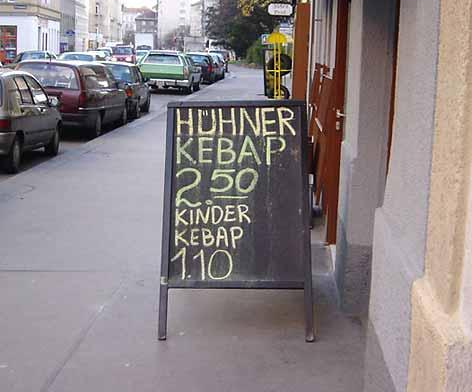
\includegraphics[scale=.55]{material/05Morph-Kebap}
%\end{figure}

\end{frame}


%%%%%%%%%%%%%%%%%%%%%%%%%%%%%%%%%%
%%%%%%%%%%%%%%%%%%%%%%%%%%%%%%%%%%
\subsubsubsection{Rektionskomposita}
%\frame{
%\frametitle{~}
%	\tableofcontents[currentsection]
%}


%%%%%%%%%%%%%%%%%%%%%%%%%%%%%%%%%%
\begin{frame}
\frametitle{Rektionskomposita}

\begin{itemize}
	\item Wichtige \textbf{Untergruppe} der Determinativkomposita:
	
	\eal \label{ex:Bsp1} 
        \ex die Linguisten tagen
        \ex die Tagung der Linguisten
        \ex Linguistentagung
	\zl
	
	\eal \label{ex:Bsp2} 
        \ex die Linguisten besteigen den Watzmann
        \ex die Besteigung des Watzmann
        \ex Watzmannbesteigung
	\zl
		 
\end{itemize}


\end{frame}


%%%%%%%%%%%%%%%%%%%%%%%%%%%%%%%%%%
\begin{frame}
\frametitle{Rektionskomposita}

\begin{itemize}
	\item \textbf{deverbale} Nomina (durch Derivation)
	
	\begin{itemize}
		\item[]
		\item tagen \ras Tagung
		\item[]
		\item Verb bestimmt mit wie vielen und mit welchen Argumenten es im Satz erscheint\\
                  (s. Rektion, Subkategorisierungsrahmen)
		
		\begin{itemize}
			\item[]
			\item Tagen in \ref{ex:Bsp1} + Subjekt
			\item[]
			\item besteigen in \ref{ex:Bsp2} + Subject + Objekt
			\item[]
			\item Beziehung zwischen Verb und seinen Argumenten auch innerhalb eines Kompositums
		\end{itemize}
	\end{itemize}
\end{itemize}


\end{frame}


%%%%%%%%%%%%%%%%%%%%%%%%%%%%%%%%%%
\begin{frame}
\frametitle{Rektionskomposita}

\begin{itemize}
	\item Rektionskompositum: \\
	die erste Konstituente in einem deverbalen Rektionskompositum realisiert ein Argument des der zweiten Konstituente zugrunde liegenden Verbs
	
	\begin{itemize}
		\item[]
		\item In \ref{ex:Bsp1}: \emph{Linguist(en)} \ras Subjekt von \emph{tagen}
		\item[]
		\item In \ref{ex:Bsp2}: Watzmann \ras Objekt von besteigen
	\end{itemize}
	
	\ea	 Auto$\cdot$fahrer (jemand fährt Auto), \\
		 Wetter$\cdot$beobachter (jemand beobachtet das Wetter), \\
		 Rotkehlchen$\cdot$gesang (das Rotkehlchen singt)
	\z
		 
\end{itemize}


\end{frame}


%%%%%%%%%%%%%%%%%%%%%%%%%%%%%%%%%%
\begin{frame}
\frametitle{Rektionskomposita}

\begin{itemize}
	\item Es gibt auch Rektionskomposita, in denen die zweite Konstituente ein nicht-deverbales Nomen oder ein Adjektiv ist, denn auch Nomina und Adjektive können Argumente nehmen:
	
	\ea Prüfungsangst (Angst vor der Prüfung), \\
		 Todessehnsucht (Sehnsucht nach dem Tod)
	\z
		 
	\ea staatstreu (dem Staat treu), \\
		 fälschungssicher (vor Fälschung sicher), \\
		 bleifrei (von Blei frei)
	\z
		 
\end{itemize}


\end{frame}


%%%%%%%%%%%%%%%%%%%%%%%%%%%%%%%%%%
\begin{frame}
\frametitle{Rektionskomposita}

\begin{itemize}
	\item \textbf{Rektionskompositum:} \\
	Kompositum, bei dem die \textbf{erste Konstituente ein Argument} (Subj., Akk.-Obj., Dat.-Obj., Gen.-Obj., Präp.-Obj., etc.) der zweiten Konstituente ist.
	\item Bei Nicht-Rektionskomposita besteht keine Argumentrelation.
\end{itemize}


\end{frame}


%%%%%%%%%%%%%%%%%%%%%%%%%%%%%%%%%%
%%%%%%%%%%%%%%%%%%%%%%%%%%%%%%%%%%
\subsubsubsection{Possessivkomposita}
%\frame{
%\frametitle{~}
%	\tableofcontents[currentsection]
%}


%%%%%%%%%%%%%%%%%%%%%%%%%%%%%%%%%%
\begin{frame}
\frametitle{Possessivkomposita}

\begin{itemize}
	\item Auch bei Possessivkomposita bestimmt die erste Konstituente die zweite näher.
	\item[]
	\item Das Kompositum bezieht sich aber auf \textbf{eine dritte Entität}, sie sind \textbf{exozentrisch}
	
	\ea \emph{Rot$\cdot$kehlchen} = Vogel, der ein rotes Kehlchen hat, nicht ein rotes Kehlchen ist
	\z
	
	\ea \emph{Rot$\cdot$käppchen} = Person, die eine rote Kappe hat (Märchenfigur), kein Käppchen
	\z
	
	\ea \emph{Lang$\cdot$finger} = Person, die lange Finger hat (= die stiehlt), kein Finger
	\z
	
\end{itemize}


\end{frame}


%%%%%%%%%%%%%%%%%%%%%%%%%%%%%%%%%%
%%%%%%%%%%%%%%%%%%%%%%%%%%%%%%%%%%
\subsubsubsection{Kopulativkomposita}
%\frame{
%\frametitle{~}
%	\tableofcontents[currentsection]
%}


%%%%%%%%%%%%%%%%%%%%%%%%%%%%%%%%%%
\begin{frame}
\frametitle{Kopulativkomposita}

\begin{itemize}
	\item Erste Konstituente \textbf{bestimmt} die zweite \textbf{nicht näher}
	\item[]
	\item Beide Konstituenten sind \textbf{gleichrangig}
	\item[]
	\item Auch aus mehr als zwei Konstituenten bestehend
	\item[]
	\item \textbf{Koordinierende} (= verknüpfende) Beziehung zwischen den Kompositionsgliedern
	\item[]
	\item Bedeutung des Kompositums ergibt sich \textbf{additiv}
	
	\eal 
	\ex süß$\cdot$sauer, nass$\cdot$kalt, rot$\cdot$grün, Fürst-Bischof
	\ex rot-rot-grün
	\zl
	
\end{itemize}


\end{frame}


%%%%%%%%%%%%%%%%%%%%%%%%%%%%%%%%%%
\begin{frame}
\frametitle{Kopulativkomposita}

\begin{itemize}
	\item Konstituenten in Kopulativkomposita \ras \textbf{gleiche Kategorie}
	\item Reihenfolge: prinzipiell frei, aber meistens \textbf{konventionalisiert}
	\item Anderes \textbf{Betonungsmuster} als Determinativkomposita
	
	\ea ein 'blau-'grünes 'Hemd - Kopulativ \\
		 ein 'blaugrünes 'Hemd - Determinativ
	\z
		 
	\item Während bei Determinativkomposita der Nichtkopf betont wird, werden bei Kopulativkomposita alle Konstituenten betont.
\end{itemize}


\end{frame}



%% \frame{
%% \frametitle{Kopulativkomposita}

%% Bei Kopulativkomposita gibt es keinen Kopf:
%% \ea
%% Fürstbischof = Fürst und Bischof gleichzeitig
%% \z

%% \pause
%% Unterschied zwischen \emph{grellweiß} und \emph{schwarz-weiß}.



%% }


\subsubsection{Derivation}


\frame{
\frametitle{Derivation}

\begin{itemize}
\item Komposition = Stamm + Stamm, Derivation = Stamm + Affix.
\pause
\item Beispiele für Regeln:

\medskip

\begin{tabular}{@{}ll@{}}
Beispiel & Regel\\
Erledigung, Beteiligung, Rechnung & N $\to$ V \suffix{ung}$_N$\\
lesbar, essbar, erklärbar & Adj $\to$ V \suffix{bar}$_{Adj}$\\
ungemütlich, unfreundlich, unschön & Adj $\to$ \prefix{un} Adj\\
Schönheit, Freiheit, Falschheit & N $\to$ Adj \suffix{heit}$_N$\\
\end{tabular}

\medskip

\pause
\item Kopf steht wieder rechts (Affixe haben Wortart)
\end{itemize}

}


\subsubsubsection{Selektion}

\frame{
\frametitle{Selektion}

Affixe gehen nicht mit beliebigem anderen Material zusammen,\\
sondern wählen sich ihren Partner aus.
\pause
\begin{itemize}
\item Wortart: \suffix{bar} verbindet sich nur mit Verben\\
      (nicht mit Adjektiven oder Nomina, bis auf unproduktive Ausnahmen)
\pause
\item Phonologische Restriktionen: \suffix{keit} verbindet sich nur mit mehrsilbigen Adjektiven, die
  auf eine unbetonte Silbe enden: \emph{Freundlichkeit}, \emph{Lesbarkeit}, \noword{Schönkeit},
  \noword{Freikeit}.
\pause
\item Bedeutung: \suffix{fach} verbindet sich nur mit Zahlen und Mengenangaben \emph{dreifach},
  \emph{mehrfach}, \noword{schönfach}, \noword{hausfach}
\pause
\item Morphologische Struktur: \gee verbindet sich nur mit morphologisch einfachen Verben
\emph{Gerenne}, \emph{Gehupe}, \noword{Geverkaufe}, \noword{Geanfange}
\end{itemize}


}

\subsubsubsection{Komplexe Verben}

\frame{
\frametitle{Komplexe Verben}

\begin{itemize}
\item Unterscheiden zwei Arten komplexer Verben: \\
Präfixverben (\emph{bestechen}, \emph{verlangen}, \emph{zersägen}) und Partikelverben
(\emph{ankaufen}, \emph{austrinken}, \emph{anlachen})
\begin{itemize}
\item Präfixverben verhalten sich wie Simplizia.
\item Partikelverben müssen in bestimmten syntaktischen bzw.\ morphologischen Umgebungen
  getrennt werden.
\eal
\ex dass Peter das Haus verkauft
\ex Peter verkauft das Haus.
\zl
\eal
\ex dass Peter das Glas austrinkt
\ex Peter trinkt das Glas aus.
\zl
\eal
\ex zersägt, zersägen
\ex ausgetrunken, auszutrinken
\zl

\end{itemize}


\end{itemize}

}


\subsubsection{Nichtkonkatenative Prozesse}

\subsubsubsection{Konversion}

\frame{
\frametitle{Nichtkonkatenative Prozesse: Konversion}


\begin{itemize}
\item Es gibt auch nichtkonkatenative Prozesse. Beispiel \blaubf{Konversion}
\item Wortart des Stammes wird geändert, ohne dass Material hinzugefügt würde.
\eal
\ex schlaf$_V$ $\to$ Schlaf$_N$
\ex grün$_{Adj}$ $\to$ grün$_{V}$
\ex braun$_{Adj}$ $\to$ bräun$_{V}$
\zl
\end{itemize}




}


\subsubsubsection{Kurzwortbildung}


\frame{
\frametitle{Kurzwortbildung und Kontamination}


\begin{itemize}
\item Kurzwortbildung
\eal
\ex Autobus $\to$ Bus
\ex Universität $\to$ Uni
\zl
\pause
\item Kontamination
\eal
\ex jein (jein = ja + nein)
\ex Teuro (teuer + Euro)
\zl


\end{itemize}





}

\subsection{Flexion}

\author{Stefan Müller (Anke Lüdeling)}

\frame[shrink=10]{
\frametitle{Flexion}

\begin{itemize}
\item Wortbildung beschäftigt sich mit Bildung neuer Lexeme.
\pause
\item Wortformen eines Lexems werden in verschiedenen Kontexten benötigt:
\begin{tabular}{@{}l@{~}l@{~}l@{~}l@{~}l@{}}
Klaus           & schmiert   & ein & belegtes & Brot.\\
Klaus           & schmierte  & ein & belegtes & Brot.\\
Klaus und Karin & schmierten & die & belegten & Brote.\\
Du              & schmierst  &     & belegte  & Brote.\\
\end{tabular}
\pause
\item Formen von \emph{schmieren} unterscheiden sich in Person, Numerus bzw.\ Tempus.
\pause
\item Formen von \emph{belegt} unterscheiden sich in Numerus und Stärke.
\pause
\item Formen von \emph{Brot} unterscheiden sich im Numerus.
\pause
\item Der Bereich, der sich mit diesen Variationen beschäftigt, heißt \alert{Flexion}.
\pause
\item Wie bei Derivation werden bei der Flexion Stämme mit einem oder mehreren Affixen kombiniert.
\pause
\item Art der Affixe hängt von Wortart ab.

\end{itemize}


}

\subsubsection{Wortarten}

\frame{
\frametitle{Wortarten}

\begin{itemize}
\item Wortarten sind Klassen von Wörtern mit ähnlichem Eigenschaften.
\pause
\item Klassische Wortarten (2. Jh. v. Chr.): Nomen, Verb, Partizip, Artikel, Pronomen, Präposition,
Adverb, Konjunktion
\pause
\item Beispiel für Definition:
\begin{quote}
Das Nomen ist ein kasusbildender Satzteil, welcher ein Ding, z.B. Stein, oder eine Handlung,
z.B. Erziehung, bezeichnet [\ldots].\\
Das Nomen hat fünf verschiedene Begleiterscheinungen:\\
Geschlecht, Art, Form, Zahl und Kasus.
\end{quote}
\pause
\item Vermischung verschiedener Kriterien aus Syntax, Semantik und Morphologie.

\pause
\item Unterscheidung zwischen flektierbaren und nichtflektierbaren Wortarten.
\end{itemize}

}


\frame{
\frametitle{Flektierbare und unflektierbare Wortarten}

\vfill
\begin{tabular}{|l|l|l|l|l|l|}\hline
\multicolumn{3}{|l|}{flektierbare Wortarten} & \multicolumn{3}{l|}{unflektierbare Wortarten}\\\hline
Name     & Abk. & Beispiele & Name         & Abk. & Beispiele\\\hline
Nomen    & N         & Tisch      & Präposition  & P         & auf, neben\\
         &           & Haus,Suppe &              &           & während\\\hline
%
Verb     & V         & koch, ess & Adverb       & Adv       & oft \\
         &           & schlaf    &              &           & gestern\\ \hline
%
Adjektiv & Adj       & schnell   & Konjunktion  & C         & dass,\\
         &           & blau      &              &           & weil,\\
         &           &           &              &           & und, oder\\\hline
%
Artikel  & D         & der, ein  & Interjektion & Int       & tja, pst, Hurra!\\\hline 
         &           &           & Partikel     & Part      & auf, an (mit Verb)\\
         &           &           &              &           & nur (drei Tage)\\\hline
\end{tabular}

\vfill

}

\subsubsubsection{Nicht flektierbare Wortarten}

\frame{
\frametitle{Nicht flektierbare Wortarten: Präpositionen}

\begin{itemize}


\item Nicht flektierbare können wir anhand ihrer syntaktischen Umgebung unterscheiden:


\alert{Präpositionen} werden mit einer Nominalgruppe kombiniert und bestimmen deren Kasus.
\eal
\ex \alert{auf} dem Sofa
\ex \alert{während} des Treffens
\zl

\pause
Präpositionalgruppen können sich auf Verben oder Nomina beziehen:
\eal
\ex die Zeitung auf dem Sofa
\ex Er schläft auf dem Sofa.
\zl

\end{itemize}

}

\frame{
\frametitle{Nicht flektierbare Wortarten: Konjunktionen}

\begin{itemize}
\item \alert{Konjunktionen} verbinden Teilsätze miteinander (\mex{1}a) oder ordnen Teilsätze einem Verb
unter (\mex{1}b):
\eal
\ex Er kommt später, \alert{weil} er noch arbeiten muss.
\ex Er glaubt, \alert{dass} er es noch schafft.
\zl

\pause
\item Auch in sogenannten Koordinationen kommen Konjunktionen vor:
\eal
\ex Er kennt \alert{und} liebt diese Schallplatte.
\ex Die Musik \alert{und} der Text ist von Frank Zappa.
\zl



\end{itemize}

}

\frame{
\frametitle{Nicht flektierbare Wortarten: Adverbien}

\alert{Adverbien} haben mehrere Funktionen.

\begin{itemize}
\item Sie modifizieren Verben (daher der Name):
\eal
\ex Max lacht \alert{oft}.
\ex Er kam \alert{gestern}.
\zl

\pause
\item Aber auch die Modifikation von Adjektiven ist möglich:
\eal
\ex das oft gelesene Buch
\ex das gestern gekaufte Buch
\zl

\pause
\item Vorsicht: Viele Adjektive können adverbial verwendet werden:
\ea
Er hat das Buch \alert{schnell} gelesen.
\z

\end{itemize}


}


\frame{
\frametitle{Nicht flektierbare Wortarten: Partikeln}

\begin{itemize}
\item Der Duden \citeyearpar{Duden2005} unterscheidet zwischen Adverbien und Partikeln.
\item \alert{Partikeln} sind wie Adverbien nicht flektierbar,\\
im Gegensatz zu Adverbien aber nicht voranstellbar:
\eal
\ex[]{
Max lacht oft.
}
\ex[]{
Oft lacht Max. (Adverb)
}
\zl
\eal
\ex[]{
Max hat sogar gelacht.
}
\ex[*]{
Sogar hat Max gelacht. (Partikel)
}
\zl
\end{itemize}

}

\frame{
\frametitle{Nicht flektierbare Wortarten: Interjektionen}

\begin{itemize}
\item  Interjektionen sind satzwertige Ausdrücke:

\begin{itemize}
\item Interjektionen im Gespräch:
\ea
Ja! Jawohl! Nein! Doch! Bitte! Danke! Servus!
              Adieu! Tschüs! Halt! Stopp! Marsch! Pst! He! Hallo!
\z

\pause
\item Interjektionen als Ausdruck von Empfindungen: 
\ea Hurra! Juchhe! Heißa! Ei!
              Bravo! Pfui! Ach! Oh! O weh! Ah! Hahaha! Potz! Hu! Hui! Iiiiii! Ätsch! Aha!
              Hm! Brrr!
\z
\pause
\item Tier- und Geräuschnachahmungen:  
\ea
Muh! Miau! Wauwau! Quak! Kikeriki!
              Knacks! Trara! Kling, klang! Piff, paff! Klipp, klapp! Plumps! Blabla!
\z
\end{itemize}
\end{itemize}

}




\subsubsubsection{Flektierbare Wortarten}

%\subsubsubsubsection{Nomina und Artikel}

\frame{
\frametitle{Nomina}


\begin{itemize}[<+->]
\item Deutsche Nomina haben ein Genus (masculin, feminin, neutrum).
\item Es gibt keine Beziehung zwischen Bedeutung und Genus (außer bei Personenbezeichnungen).
\item Genus ändert sich nicht in Abhängigkeit vom syntaktischen Kontext.\\
      Bezeichnung: \alert{inheränte Flexionskategorie}.
\item Abhängig vom Kontext Flexion nach Numerus (singular, Plural) und Kasus (Nominativ, Genitiv,
Dativ, Akkusativ).

\medskip


\begin{tabular}{|l|l|l|l|l|l|l|}\hline
          & \multicolumn{3}{l|}{Singular} & \multicolumn{3}{l|}{Plural}\\\hline
Nominativ & Tisch   & Suppe & Haus   & Tische  & Suppen & Häuser\\\hline
Genitiv   & Tisches & Suppe & Hauses & Tische  & Suppen & Häuser\\\hline
Dativ     & Tisch   & Suppe & Haus   & Tischen & Suppen & Häusern\\\hline
Akkusativ & Tisch   & Suppe & Haus   & Tische  & Suppen & Häuser\\\hline
\end{tabular}
\end{itemize}

}

\author{Stefan Müller}

\frame[shrink]{
\frametitle{Pronomina und Artikelwörter}


\begin{itemize}
\item Pronomina und Artikelwörter bilden eine Restkategorie.
\pause
\item Der Begriff \emph{Pronomen} kommt aus der Grammatik des Latein und steht
      traditionell sowohl für Artikel als auch für Wörter, die ganze Nominalgruppen ersetzen.
\pause
\item Das war sinnvoll, denn die Formen waren identisch.

Sie haben sich aber historisch auseinanderentwickelt.

\pause
\item Statt \emph{Pronomen} im obigen Sinn verwenden Grammatiken die stärker differenzierenden Begriffe \alert{Stellvertreter} und \alert{Begleiter}.

\pause
\item \alert{Artikel}/\alert{Determinator}: Element, das mit Nomen bzw.\ Adjektiven eine Nominalgruppe bildet
\pause
\item \alert{Pronomen}: Element, das für eine Nominalgruppe steht.

Zu den Pronomina werden auch die sogenannten Pronominaladverbien (\emph{darüber}, \emph{damit}, \ldots).

Diese stehen für Präpositionalgruppen (\emph{über dem Tisch}).
\end{itemize}

}

% \frame{
% \frametitle{Unterschied: definiter Artikel und Demonstrativpronomen}


% Die Formen des definiten Artikels und des Demonstrativpronomens sind meistens identisch,
% jedoch nicht immer:

% \medskip

% \begin{tabular}{|l|l|l|}\hline
% Kasus & Definiter Artikel & Demonstrativpronomen \\\hline
% Nom & der Mann   & der\\
% Gen & \alert{des} Mannes & \alert{dessen}\\
% Dat & dem Mann   & dem\\
% Akk & den Mann   & den\\\hline
% Nom & die Manner & die\\
% Gen & \alert{der} Männer & \alert{derer}\\
% Dat & \alert{den} Männern & \alert{denen}\\
% Akk & die Männer  & die\\\hline
% \end{tabular}


% }


\frame[shrink]{
\frametitle{Artikel/Determinator}

\begin{itemize}
\item Artikel stehen vor Nomina (oder Adjektiven) und bestimmen Definitheit:
\eal
\ex das/dieses/jenes Haus
\ex ein/kein Haus
\ex einige/mehrere Häuser
\zl

\pause
\item Klassisch: \alert{definiter Artikel} = \emph{der}, \emph{die}, \emph{das}
      \alert{indefiniter Artikel} = \emph{ein}

Duden-Grammatik nennt \emph{etwas}, \emph{nichts}, \emph{einige} \alert{indefinite Artikelwörter}
\eal
\ex etwas Farbe
\ex nichts Süßes
\ex einige Minuten
\ex alle Leute
\ex irgendwelche Kollegen
\zl

\end{itemize}

}

\author{Stefan Müller (Anke Lüdeling)}

\frame{
\frametitle{Artikel/Determinator: Flexionskategorien}

\begin{itemize}
\item Artikel haben dieselben Flexionskategorien wie Nomina.


\medskip


\begin{tabular}{|l|l|l|l|l|}\hline
          & \multicolumn{3}{l|}{Singular} & Plural\\\hline
Nominativ & der & die & das & die\\\hline
Genitiv   & des & der & des & der\\\hline
Dativ     & dem & der & dem & den\\\hline
Akkusativ & den & die & das & die\\\hline
\end{tabular}
\end{itemize}

}

\frame{
\frametitle{Synkretismus}

\begin{itemize}
\item Die Pluralformen sind für alle drei Genera identisch:

\medskip

\begin{tabular}{|l|l|l|l|l|}\hline
          & \multicolumn{3}{l|}{Singular} & Plural\\\hline
Nominativ & der & die & das & die\\\hline
Genitiv   & des & der & des & der\\\hline
Dativ     & dem & der & dem & den\\\hline
Akkusativ & den & die & das & die\\\hline
\end{tabular}

~

\pause
\item Auch im nominalen Paradigma fallen viele Formen zusammen.

Diesen Zusammenfall von Formen nennt man \alert{Synkretismus}.

\pause
\item Kasus lässt sich nicht eindeutig von der Form ablesen.

Kombination der Information von Artikel und Nomen hilft mitunter:
\eal
\ex der Tisch
\ex dem Tisch
\zl
\end{itemize}

}

\author{Stefan Müller}

\frame{
\frametitle{Synkretismus und Sexismus}

\begin{itemize}
\item Das hilft aber bei femininen Nomina nicht:
\ea
die Tochter (Nominativ oder Akkusativ)
\z
\pause

In Beispielen werden deshalb oft maskuline Nomina verwendet.

Kein Sexismus, sondern Vermeidung von Mehrdeutigkeit.

\pause
\item Meist hilft der Kontext, die Abfolge der Nominalgruppen im Satz oder die Prosodie:
\eal
\ex Den Vater liebt die Tochter nicht. Die Mutter liebt die Tochter.
\ex Die Mutter liebt den Sohn nicht. Die Mutter liebt die Tochter.
\zl

\end{itemize}

}


%{Pronomina}
\frame{
\frametitle{Pronomina -- I}

\begin{itemize}
\item \alert{Personalpronomen} (persönliche Fürwörter):\\
\emph{ich}, \emph{du}, \emph{er}, \emph{sie}, \emph{es}, \emph{wir}, \emph{ihr}, \emph{sie}

\pause
\item \alert{Possessivpronomen} (besitzanzeigende Fürwörter):\\
\emph{mein}, \emph{dein}, \emph{sein}, \emph{unser}, \emph{euer}, \emph{ihr}

\pause
\item \alert{Reflexivpronomen} (rückbezügliche Fürwörter):\\
\emph{mich}, \emph{dich}, \emph{sich}, \emph{uns}, \emph{euch}

\ea
Ich erhole \alert{mich}.
\z

\pause
\medskip
Reflexiv gebrauchtes Personalpronomen: auch Dativformen

\eal
\ex Ich wasche \alert{mich}.
\ex Ich wasche \alert{mir} den Rücken.
\zl

\pause
\alert{Reziprokpronomen} (wechselseitige Fürwörter): \emph{einander}

\end{itemize}


}


\frame{
\frametitle{Pronomina -- II}

\begin{itemize}

\item \alert{Demonstrativpronomen} (hinweisende Fürwörter):\\

    \emph{der}, \emph{dieser}, \emph{jener}, \emph{derjenige}, \emph{derselbe},\\
    \emph{die}, \emph{diese}, \emph{jene}, \emph{diejenige}, \emph{dieselbe},\\
    \emph{das}, \emph{dieses}, \emph{jenes}, \emph{dasjenige}, \emph{dasselbe}

\pause
\item \alert{Relativpronomen} (bezügliche Fürwörter):\\
\emph{der}, \emph{die}, \emph{das}, \emph{welcher}, \emph{welches}, \emph{welche},\\

\emph{wer}, \emph{was} (in freien Relativsätzen)

\pause
\item \alert{Interrogativpronomen} (fragende Fürwörter):\\
\emph{wer}, \emph{was}, \emph{welcher}

\pause
Frageadverbien auch hier einordnen? \emph{wofür}, \emph{womit}

\pause
\item \alert{Indefinitpronomen} (unbestimmte Fürwörter):\\
\emph{jemand}, \emph{alle}, \emph{einer}, \emph{keiner}, \emph{mancher}, \emph{man}, \emph{wer}, \emph{etwas}, \ldots

\end{itemize}


}

\author{Stefan Müller (Anke Lüdeling)}

\frame{
\frametitle{Adjektive: Flexionsklasse}

\begin{itemize}
\item Adjektive modifizieren Nomina (\mex{1}a) o.\ werden prädikativ verwendet (\mex{1}b):
\eal
\ex das rote Haus
\ex Das Haus ist rot.
\zl

\pause
\item Wie bei Nomina nach Kasus, Genus, Numerus unterschieden.
\pause
\item Zusätzlich Flexionsklasse: stark, schwach, gemischt:
\eal
\ex leckerer Auflauf, leckere Aufläufe\\ (ohne Artikel = stark)
\pause
\ex der leckere Auflauf, die leckeren Aufläufe\\ (definit = schwach)
\pause
\ex ein leckerer Auflauf, einige leckere Aufläufe\\ (ein/kein = gemischt)
\zl
\end{itemize}

}


\frame{
\frametitle{Adjektive: Grad}

\begin{itemize}
\item Flexion nach Grad:
\begin{itemize}
\item Positiv: \emph{lecker}
\item Komparativ: \emph{leckerer}
\item Superlativ: \emph{am leckersten}
\end{itemize}
\pause
\item Das ganze Paradigma unter \url{http://www.canoo.net/}.
\end{itemize}


}

\frame{
\frametitle{Verben}

\begin{itemize}
\item Verben unterteilen sich in Vollverben, Hilfsverben (Auxiliare) und Modalverben.
\pause
\item Vollverben teilen sich in schwache (regelmäßige) und starke (unregelmäßige) auf.\\
      Stark vs.\ schwach unterscheidet sich von den Klassen bei Adjektiven.
\pause
\item Vollverben und Hilfsverben flektieren nach Person, Numerus, Tempus, Modus und Genus Verbi.
\pause
\item Person und Nummerus sind für den syntaktischen Kontext wichtig (Kongruenz):

\medskip

~
\begin{tabular}{@{}lll@{}}
           & Singular  & Plural\\
1.\ Person & ich lache & wir lachen\\
2.\ Person & du lachst & ihr lacht\\
3.\ Person & er/sie/es lacht & sie lachen\\
\end{tabular}
\end{itemize}

}


\frame{
\frametitle{Verben: Tempus}

\begin{itemize}
\item Tempus, Modus und Genus Verbi fügen semantische Information hinzu.

\pause
\item Vereinfacht: Tempus sagt etwas darüber aus, wann die Handlung stattfindet.
\ea
Er lachte / lacht / wird lachen.
\z
\pause
\item Allerdings kann Präsens auch in Sätzen benutzt werden, die die Vergangenheit oder Zukunft beschreiben:
\eal
\ex Napoleon wird 1769 in Ajaccio auf der Insel Korsika geboren.
\ex Kommt er gestern in die Küche
\ex Ich bringe den Müll morgen runter.
\zl

\pause
\item Es gibt morphologisch einfache Formen und zusammengesetzte mit Hilfsverb + Partizip/Infinitiv.

\end{itemize}

}



\frame{
\frametitle{Flexionsparadigma: schwaches Verb, Aktiv, Indikativ}

\oneline{\begin{tabular}{|l|l|l|l|l|l|l|}\hline
Person \& & Präsens & Präteri- & Perfekt & Plusquam- & Futur I & Futur II\\
Numerus   &         & tum      &         & perfekt   &         &         \\\hline
%
1.\ Sg    & koche   & kochte   & habe    & hatte     & werde   & werde \\
          &         &          & gekocht & gekocht   & kochen  & gekocht haben\\\hline
%
2.\ Sg    & kochst  & kochtest & hast    & hattest   & wirst   & wirst \\
          &         &          & gekocht & gekocht   & kochen  & gekocht haben\\\hline
%
3.\ Sg    & kocht   & kochte   & hat     & hatte     & wird    & wird\\
          &         &          & gekocht & gekocht   & kochen  & gekocht haben\\\hline
%
1.\ Pl    & kochen  & kochten  & haben   & hatten    & werden & werden\\
          &         &          & gekocht & gekocht   & kochen & gekocht haben\\\hline
%
2.\ Pl    & kocht   & kochtet  & habt    & hattet    & werdet & werdet\\
          &         &          & gekocht & gekocht   & kochen & gekocht haben\\\hline
%
3.\ Pl    & kochen  & kochten  & haben   & hatten    & werden & werden\\
          &         &          & gekocht & gekocht   & kochen & gekocht haben\\\hline
\end{tabular}}


}

\frame{
\frametitlefit{Flexionsschema: schwache Verben, Präsens, Indikativ, Aktiv}


\vfill

\hfill
\begin{tabular}{|l|l|l|}\hline
Person \& & \multicolumn{2}{c|}{Präsens}\\
Numerus   &  \multicolumn{2}{c|}{} \\\hline
%           
1.\ Sg    &        & \suffix{e}\\\cline{1-1}\cline{3-3}
%           
2.\ Sg    &        & \suffix{st}\\\cline{1-1}\cline{3-3}
%           
3.\ Sg    &        & \suffix{t}\\\cline{1-1}\cline{3-3}
%           
1.\ Pl    & Stamm  & \suffix{en}\\\cline{1-1}\cline{3-3}
%           
2.\ Pl    &        & \suffix{t}\\\cline{1-1}\cline{3-3}
%           
3.\ Pl    &        & \suffix{en}\\\hline
\end{tabular}\hfill\hfill\mbox{}

\vfill

}

\frame{
\frametitle{Modus}


\begin{itemize}
\item Verbmodus: Indikativ, Konjunktiv I, Konjunktiv II
\pause
\item Bedeutung unscharf, kann aber wie folgt umrissen werden:
\begin{itemize}
\item Indikativ teilt Faktum mit
\ea
Max schläft. (Ich habe es selbst gesehen.)
\z
\pause
\item Konjunktiv I: Man hat von etwas gehört.
\ea
Barbara sagt, Max schlafe. (Ich glaube Barbara.)
\z
\pause
\item Konjunktiv II: Man hat von etwas gehört und zweifelt es an.
\ea
Barbara sagt, Max schliefe. (Ich glaube Barbara nicht.)
\z
\end{itemize}
\end{itemize}


}


\frame{
\frametitle{Genus Verbi}




\begin{itemize}
\item Genus Verbi: Aktiv und Passiv

\eal
\ex Er schlägt den Weltmeister.
\ex Der Weltmeister wird geschlagen.
\zl
\pause
\item Passiv = Unterdrückung des Subjekts (Agens im weiteren Sinne)
\pause
\item Die häufigste Form des Passivs wird mit dem Hilfsverb \emph{werden} gebildet.

\end{itemize}

}

\frame{
\frametitle{Andere Verbformen}


\eal
\ex geben (Infinitiv)
\pause
\ex gebend (Partizip Präsens)
\pause
\ex gegeben (Partizip Perfekt)
\pause
\ex gib (Imperativ Singular)
\pause
\ex gebt (Imperativ Plural)
\zl


}

\frame{
\frametitle{Modalverben und \emph{wissen}}


\begin{itemize}
\item Modalverben (\emph{dürfen}, \emph{können}, \emph{mögen}, \emph{müssen}, \emph{sollen}, \emph{wollen}),\\
      und damit gebildete Präfix- oder Partikelverben (\emph{bedürfen}, \emph{durchmüssen})\\
      und das Verb \emph{wissen} verhalten sich etwas anders.
\item Im Präsens verwenden sie die Präteritumsendungen der starken Verben.

~

\vfill


\hfill
\begin{tabular}{|l|l|l|l|l|}\hline
Person \& & \multicolumn{2}{c|}{Präteritum starke Verben} & \multicolumn{2}{c|}{Präsens Modalverben}\\
Numerus   &  \multicolumn{2}{c|}{} & \multicolumn{2}{c|}{} \\\hline
%           
1.\ Sg    &                  & $\varnothing$    && $\varnothing$    \\\cline{1-1}\cline{3-3}\cline{5-5}
%                                                                                    
2.\ Sg    & Präteritumsstam  & \suffix{st}      & Stamm & \suffix{st}      \\\cline{1-1}\cline{3-3}\cline{5-5}
%                                                                                    
3.\ Sg    & \emph{kam}       & $\varnothing$    & \emph{darf}/\emph{dürf}& $\varnothing$    \\\cline{1-1}\cline{3-3}\cline{5-5}
%                                                                                    
1.\ Pl    & \emph{schlief}   & \suffix{en}      & \emph{will}/\emph{woll} & \suffix{en}      \\\cline{1-1}\cline{3-3}\cline{5-5}
%                                                                                    
2.\ Pl    &                  & \suffix{t}       && \suffix{t}       \\\cline{1-1}\cline{3-3}\cline{5-5}
%                                                                                    
3.\ Pl    &                  & \suffix{en}      && \suffix{en}      \\\hline
\end{tabular}\hfill\hfill\mbox{}

\vfill

\end{itemize}

}

\subsubsubsection{Überblick}

\author{Stefan Müller (Peter Gallmann)}

\frame{
\frametitle{Überblick über die Wortarten (Peter Gallmann/Duden)}

\vfill

% used to work without tabular, I do not know why it needs tabular here. Maybe order of loading of packages
\centerfit{%
\begin{forest}
word tier, for tree={fit=rectangle}
[Wortart
       [flektierbar
          [nach Tempus [Verb] ]
          [nach Kasus 
            [festes Genus [Noun] ]
            [veränderbares Genus 
               [nicht komparierbar [\begin{tabular}{@{}c@{}}Artikelwort\\Pronomen\end{tabular} ] ]
               [komparierbar [Adjektiv] ] ] ] ]
       [nicht flektierbar [\begin{tabular}{@{}c@{}}Adverb\\Konjunktion\\Präposition\\Interjektion\end{tabular}] ] ]
\end{forest}
}

\vfill

}

\author{Stefan Müller (Anke Lüdeling)}

\subsubsection{Form und Funktion}

\frame{
\frametitle{Form und Funktion: Portmanteau-Morpheme}

\begin{itemize}
\item Wortbildung: Jedes Morphem hat eine Funktion/Bedeutungsbeitrag:
\eal
\ex Haus+tür
\ex Stör+ung
\zl

\pause
\item Flexion: Mitunter fallen mehrere Funktionen zusammen:
\eal
\ex ich lache -- lachte
\ex er lacht -- lachte
\zl
Steht das \suffix{t} für Präteritum, wie (\mex{0}a) nahelegt?

\pause
Steht das \suffix{e} für Präteritum, wie (\mex{0}b) nahelegt?

\pause
\item \suffix{te} ist ein kombiniertes Affix,\\
      das sowohl Tempus- als auch Kongruenzinformation enthält.

Solche Morpheme werden \alert{Portmanteau-Morpheme} oder \alert{Schachtelmorpheme} genannt.

\end{itemize}

}

\frame{
\frametitle{Form und Funktion: mehrfache Exponenten}

\begin{itemize}
\item Bei Portmanteau-Morphemen werden mehrere Funktionen von einem Morphem wahrgenommen.
\pause
\item Aber es gibt auch Fälle, in denen eine Funktion sich an mehreren Stellen manifestiert.

Beispiel: bestimmte Nomina im Deutschen, die mit Suffix und Umlautung den Plural bilden:
\ea
Mann -- Männer
\z
\end{itemize}

}



\frame{
\frametitle{Inhärente Flexion, regierte Flexion und Kongruenz}

\begin{itemize}
\item Flexion hilft bei der Bestimmung der Zusammengehörigkeit und Funktion von Elementen im Satz.
\item Können Flexionsinformation unterteilen in 
\begin{itemize}
\item inhärente Flexion, 
\item kontextabhängige Flexion,
\item regierte Flexion und 
\item Kongruenz

\end{itemize}

\end{itemize}

}

\frame{
\frametitle{Inhärente und kontextuelle Kategorien}

\begin{itemize}
\item Inhärente Flexionskategorien, \zb Genus bei Nomina oder Definitheit bei Artikeln: Diese
Informationen gehören zum Lexem, sie ändern sich nie. 

Sie können aber durchaus Auswirkungen auf andere Elemente in ihrer Umgebung haben.

\pause
\item Kontextuelle Kategorien, \zb Modus oder Tempus bei Verben. Solche Kategorien sind nicht durch
die Syntax vorgegeben, sondern durch das Informationsziel. 

\end{itemize}



}

\frame{
\frametitle{Regierte Flexion}

Regierte Kategorien, \zb Kasus bei nominalen Konstituenten in einer präpositionalen
Konstituente. 
\ea
in einem Korb
\z

Regierendes Element (\emph{in}) verlangt Dativ, steht aber nicht selbst im Dativ.

Durch Rektion wird Abhängigkeit aufgezeigt:\\
Alles, was von der Präposition abhängt, muss im Dativ stehen.
}

\frame{
\frametitle{Kongruenz}

Kongruenz: ein Element stimmt mit anderen Elementen in seiner Umgebung in einem oder mehreren
Merkmalen überein. 

\eal
\ex Max lacht.
\ex Max und Friederike lachen.
\zl
\eal
\ex ein gutes Ergebnis
\ex das gute Ergebnis
\ex des guten Ergebnisses
\zl

}

\subsection{Übung Derivation, Komposition, Flexion}

\frame{
\frametitle{Übung}

Analysieren Sie:
\eal
\ex Vorlesungsankündigung
\ex Straßenbahnhaltestelle
\ex Kinderschlafsack
\ex Kinderschreibtische
\zl

}

\frame{
\frametitle{Lösung: Vorlesungsankündigung}

\centerline{
\begin{forest}
sm edges
[N
  [N
    [N 
      [V 
        [Part [vor]]
        [V [les]]]
      [N-Aff [ung-s]]]
    [N [V [Part [an]]
          [V [kündig]]]
       [N-Aff [ung]]]]
  [Flex [$\varnothing$]]]
\end{forest}
}

\emph{kündigen}: mhd. für `mitteilen, künden'

}


\frame{
\frametitle{Lösung: Straßenbahnhaltestelle}

\centerline{%
\begin{forest}
sm edges
[N 
  [N
    [N
      [N [Straße-n]]
      [N [bahn]]]
    [N [V [halt-e]]
       [N [stelle]]]]
  [Flex [$\varnothing$]]]
\end{forest}}

}

\frame{
\frametitle{Lösung: Kinderschlafsack}

\centerline{%
\begin{forest}
sm edges
[N
  [N [N [kind-er]]
     [N
       [V [schlaf]]
       [N [sack]]]]
  [Flex [$\varnothing$]]]
\end{forest}
}

}

\frame{
\frametitle{Lösung: Kinderschreibtische}

\centerline{%
\begin{forest}
sm edges
[N
  [N [N [kind-er]]
     [N
       [V [schreib]]
       [N [tisch]]]]
  [Flex [e]]]
\end{forest}
}

}



%% -*- coding:utf-8 -*-

\subsection{Hausaufgaben}

\begin{frame}
	\frametitle{Hausaufgaben}

	
\begin{enumerate}
	 \item Kreuzen Sie die korrekten Aussagen an: %\hfill(0,5 Punkte pro Aussage)\\

\begin{itemize}
	\item[$\circ$] Die Graphemkette \emph{abarbeiten} ist ein einzelnes phonologisches Wort im Deutschen.
	\item[$\circ$] \emph{Morphologieeinführungsbuch} ist ein orthographisch-graphemisches Wort des Deutschen, sowie \emph{introductory morphology book} ein orthographisch-graphemisches Wort des Englischen ist.
	\item[$\circ$] Ein Morphem ist die kleinste bedeutungsunterscheidende Einheit in einem bestimmten Sprachsystem.
	\item[$\circ$] \ab{Brot} und \ab{Bröt} sind Allomorphe eines einzelnen Morphems.
\end{itemize}

	\item Erklären Sie das Prinzip der Rechtsköpfigkeit in der Morphologie des Deutschen. Verwenden Sie bei Ihrer Erklärung die unten angegebenen Beispiele.%\hfill(4 Punkte)\\

\eal
\ex lichtblau, Blaulicht
\ex die Fotowelt, das Weltfoto
\ex der Bücherrücken/die Bücherrücken, das Rückenbuch/die Rückenbücher
\zl
\end{enumerate}

\end{frame}



\begin{frame}
\frametitle{Hausaufgaben}
\begin{itemize}
	\item[3.] Geben Sie Argumente für oder gegen die Behandlung von \emph{ver-} in den folgenden Wörtern als Morphem an. Wenn es sich um ein Morphem handelt, ist das immer das gleiche Morphem? %(4 Punkte)

	\eal
	\ex \emph{Ver}zweiflung
	\ex \emph{Ver}s
	\ex \emph{ver}kaufen
	\ex \emph{ver}schreiben
	\ex \emph{ver}fahren
	\zl

\end{itemize}
\end{frame}



\begin{frame}
	\frametitle{Hausaufgaben}
	
\begin{itemize}
\item[4.] Ordnen Sie die Wortbildungsprozesse links den passenden Beispielen rechts zu (dazu müssen Sie nur den entsprechenden Buchstaben neben das passende Beispiel schreiben). %(0,5 Punkte pro Aussage)
\end{itemize}

\begin{table}[h!]
	\begin{minipage}{0.4\linewidth}
		\centering
		\begin{tabular}{l|p{0.1\textwidth}|}
			Determinativkompositum & (A)\\
			\hline
			Konversion & (B)\\
			\hline
			Zirkumfigierung (Derivation) & (C)\\
			\hline
			Rektionskompositum & (D)\\
			\hline
			Possessivkompositum & (E)\\
		\end{tabular}
		
	\end{minipage}\hfill%
	\begin{minipage}{0.4\linewidth}
		\centering
		\begin{tabular}{|p{0.1\textwidth}|r}
			& \emph{Gerede} \\
			\hline
			& \emph{Milchgesicht}\\
			\hline
			& \emph{Lauf} \\
			\hline
			& \emph{Kettenraucher}  \\
			\hline
			& \emph{Klausurbesprechung}  \\
		\end{tabular}
	\end{minipage}
\end{table}
\end{frame}



\begin{frame}
	\frametitle{Hausaufgaben}
\begin{itemize}
\item[5.] Warum sind die Wörter unter (i.) grammatisch und die unter (ii.) ungrammatisch? %(4 Punkte)
	\eal
	\ex kaufbar, trinkbar
	\ex *fensterbar, *helfbar, *schönbar
	\zl

      \item [6.] Sind die folgenden Verben Präfixverben oder Partikelverben? Begründen Sie Ihre Entscheidungen. %(3 Punkte)

	\eal
	\ex auskennen
	\ex erkennen
	\ex aberkennen
	\zl

\item [7.] Geben Sie für das folgende Wort eine morphologische Konstituentenstruktur (inklusive Konstituentenkategorien (N, N\textsuperscript{af}, V, V\textsuperscript{af}, \dots)) an, und bestimmen Sie für jeden Knoten den Wortbildungstyp. %(6,5 Punkte)

	\ea
	Wahlkampfberaterinnen
	\z

\end{itemize}

\end{frame}



\begin{frame}
	\frametitle{Hausaufgaben}
	
\begin{itemize}

\item [8.] Paraphrasieren Sie das folgende komplexe Wort so, dass es der angegebenen Struktur entspricht (auch wenn Sie selbst eine andere Struktur plausibler finden sollten). %(2 Punkte)

\begin{forest}sn edges,
	[N
	[N[N[Reserve]]
	[N[V[lehr]][N\textsuperscript{af}[-er]]]]
	[N[zimmer]]
	]
\end{forest}

\end{itemize}

\end{frame}


\begin{frame}
	\frametitle{Hausaufgaben}
	
\begin{itemize}

\item [9.] Geben Sie für die folgende Wortform die Flexionskategorien an, nach denen sie flektiert ist.\\
%\hfill(3 Punkte)\\
	\ea
	bestehe
	\z

\end{itemize}

\end{frame}

%%%%%%%%%%%%%%%%%%%%%%%%%%%%%%%%%%%%%%%%%%%%%%%%%%%%%%%%%%%%%%
%%%%%%%%%%%%%%%%%%%%%%%%%%%%%%%%%%%%%%%%%%%%%%%%%%%%%%%%%%%%%
\subsection{Lösungen}
%%%%%%%%%%%%%%%%%%%%%%%%%%%%%%%%%%%%%%%%%%%%%%%%%%%%%%%%%%%%%%
%%%%%%%%%%%%%%%%%%%%%%%%%%%%%%%%%%%%%%%%%%%%%%%%%%%%%%%%%%%%%
\begin{frame}
	\frametitle{Lösungen}

\begin{enumerate}
	\item Kreuzen Sie die korrekten Aussagen an: %\hfill(0,5 Punkte pro Aussage)\\
	
	\begin{itemize}
	\item[$\circ$] Die Graphemkette abarbeiten ist ein einzelnes phonologisches Wort im Deutschen.
	\item[$\circ$] \emph{Morphologieeinführungsbuch} ist ein orthographisch-graphemisches Wort des Deutschen, sowie \emph{introductory morphology book} ein orthographisch-graphemisches Wort des Englischen ist.
	\item[$\circ$] Ein Morphem ist die kleinste bedeutungsunterscheidende Einheit in einem bestimmten Sprachsystem.
	\textcolor{red}{\item[$\checkmark$] \ab{Brot} und \ab{Bröt} sind Allomorphe eines einzelnen Morphems.}
\end{itemize}
	
	\item Erklären Sie das Prinzip der Rechtsköpfigkeit in der Morphologie des Deutschen. Verwenden Sie bei Ihrer Erklärung die unten angegebenen Beispiele.%\hfill(4 Punkte)\\
	
		\eal
			\ex lichtblau, Blaulicht \ras Wortart
			\ex die Fotowelt, das Weltfoto \ras Genus und Semantik
			\ex der Bücherrücken/die Bücherrücken, das Rückenbuch/die Rückenbücher \ras Pluralflexion
		\zl		
\end{enumerate}

\end{frame}

%%%%%%%%%%%%%%%%%%%%%%%%%%%%%%%%%%%%%%%%%%%%%%%%%%%%%%%%%%%%

\begin{frame}
\frametitle{Lösungen}
\begin{itemize}
	\item[3.] Geben Sie Argumente für oder gegen die Behandlung von \emph{ver-} in den folgenden Wörtern als Morphem an. Wenn es sich um ein Morphem handelt, ist das immer das gleiche Morphem? %(4 Punkte)
	
	\eal \label{ver}
	\ex\label{vera}  \emph{Ver}zweiflung
	\ex\label{verb} \emph{Ver}s
	\ex \label{verc} \emph{ver}kaufen
	\ex\label{verd}  \emph{ver}schreiben
	\ex\label{vere} \emph{ver}fahren
	\zl
	
	\textcolor{red}{
		Morphem: Kleinste bedeutungstragende Einheit im Sprachsystem.	
		\begin{itemize}
			\item[] \gqq{ver} in (\ref{verb})  \ras kein Morphem, sondern Bestandteil des Stammes.
			\item[] \gqq{ver} in (\ref{ver}a,c,d,e) \ras Morpheme, aber unterschiedliche Morpheme, weil sie unterschiedliche Bedeutungen tragen
			\item[] \gqq{ver} in (\ref{ver}d,e) trägt die Bedeutung \gq{X falsch machen} (d.h. \gq{falsch schreiben/fahren})
			\item[] \gqq{ver} in (\ref{verc}) kehrt die Bedeutung von X um (kaufen \ras verkaufen)
			\item[] \gqq{ver} in (\ref{vera}) trägt eine intensivierende(?) Bedeutung
		\end{itemize}
	}
\end{itemize}
\end{frame}

%%%%%%%%%%%%%%%%%%%%%%%%%%%%%%%%%%%%%%%%%%%%%%%%%%%%%%%%%%%%

\begin{frame}
\frametitle{Lösungen}

\begin{itemize}
	\item[4.] Ordnen Sie die Wortbildungsprozesse links den passenden Beispielen rechts zu (dazu müssen Sie nur den entsprechenden Buchstaben neben das passende Beispiel schreiben). %(0,5 Punkte pro Aussage)
\end{itemize}

	\begin{table}[h!]
	\begin{minipage}{0.4\linewidth}
		\centering
		\begin{tabular}{|l|p{0.1\textwidth}|}
			\hline 
			Determinativkompositum & (A)\\
			\hline
			Konversion & (B)\\
			\hline
			Zirkumfigierung (Derivation) & (C)\\
			\hline
			Rektionskompositum & (D)\\
			\hline
			Possessivkompositum & (E)\\
			\hline 
		\end{tabular}
		
	\end{minipage}\hfill%
	\begin{minipage}{0.4\linewidth}
		\centering
		\begin{tabular}{|p{0.1\textwidth}|r|}
			\hline 
			\textcolor{red}{C} & \emph{Gerede} \\
			\hline
			\textcolor{red}{E} & \emph{Milchgesicht}\\
			\hline
			\textcolor{red}{B} & \emph{Lauf} \\
			\hline
			\textcolor{red}{A} & \emph{Kettenraucher}  \\
			\hline
			\textcolor{red}{D} & \emph{Klausurbesprechung}  \\
			\hline 
		\end{tabular}
	\end{minipage}
\end{table}
\end{frame}

%%%%%%%%%%%%%%%%%%%%%%%%%%%%%%%%%%%%%%%%%%%%%%%%%%%%%%%%%%%

\begin{frame}
\frametitle{Lösungen}
\begin{itemize}
	\item[5.] Warum sind die Wörter unter (\ref{kauf}) grammatisch und die unter (\ref{fenster}) ungrammatisch? %(4 Punkte)
	\eal
	\ex\label{kauf} kaufbar, trinkbar
	\ex\label{fenster} *fensterbar, *helfbar, *schönbar
	\zl
	
	\textcolor{red}{
		Das Suffix \gqq{-bar} hat die folgenden Beschränkungen bzgl. der Basis X, mit der es sich verbindet:
		\begin{itemize}
			\item[] X muss ein Verb sein (nicht Nomen oder Adjektiv)
			\item[] X muss transitiv sein (nicht wie \gqq{helfen})
		\end{itemize}
	}

	\item [6.] Sind die folgenden Verben Präfixverben oder Partikelverben? Begründen Sie Ihre Entscheidungen. %(3 Punkte)
	
	\eal
	\ex auskennen
	\ex erkennen
	\ex aberkennen
	\zl
	
	\textcolor{red}{
		Partikelverb: 1) morphologisch trennbar (\emph{aus-ge-kannt}, \emph{ab-zu-erkennen}), 2) syntaktisch trennbar (\gqq{Peter \emph{kennt} sich \emph{aus}}, \gqq{Die Frau \emph{erkennt} die Urkunde \emph{ab}}) und 3) die Partikel trägt die Hauptbetonung (\emph{AUSkennen} und \emph{ABerkennen}).
		Präfixverb: weder morphologisch noch syntaktisch trennbar (*\emph{ergekannt}, \gqq{*\emph{Peter kannte ihn er}}), Hauptbetonung liegt auf der Basis (\emph{erKENnen}).\\
		\bigskip
		EXTRA: \gqq{aberkennen} ist ein Partikelverb, welches aus einem Präfixverb und einer Partikel besteht (ab+erkennen).\\
	}
\end{itemize}

\end{frame}

%%%%%%%%%%%%%%%%%%%%%%%%%%%%%%%%%%%%%%%%%%%%%%%%%%%%%%%%%%%

\begin{frame}
	\frametitle{Lösungen}
	\item [7.] Geben Sie für das folgende Wort eine morphologische Konstituentenstruktur (inklusive Konstituentenkategorien (N, N\textsuperscript{af}, V, V\textsuperscript{af}, \dots)) an, und bestimmen Sie für jeden Knoten den Wortbildungstyp. %(6,5 Punkte)

\ea
Wahlkampfberaterinnen
\z

\textcolor{red}{
	%	\begin{figure}[h]
	\begin{forest} MyP edges,
		[N, name=N1
		[N, name=N2
		[N, name=N3
		[N, name=N4
		[N, name=N6 [V[wahl/wähl]]]
		[N, name=N7 [V[kampf/kämpf]]]]
		[N, name=N5[V, name=V1	[V\textsubscript{af}[be-]]
		[V[rat]]]
		[N\textsuperscript{af}[-er]]]]
		[N\textsuperscript{af}[-in]]]
		[Fl[-nen]]]	
		{
			\draw[<-, red] (N1.west)--++(-10em,0pt)
			node[anchor=east,align=center]{Flexion (KEIN Wortbildungsporzess)};
			\draw[<-, red] (N2.west)--++(-12em,0pt)
			node[anchor=east,align=center]{Derivation (Movierung)};
			\draw[<-, red] (N3.west)--++(-8em,0pt)
			node[anchor=east,align=center]{Determinativkompositum};
			\draw[<-, red] (N4.west)--++(-3em,0pt)
			node[anchor=east,align=center]{Determinativkompositum};
			\draw[<-, red] (N5.west)--++(-2em,0pt)
			node[anchor=east,align=center]{Derivation};
			\draw[<-, red] (N6.west)--++(-2em,0pt)
			node[anchor=east,align=center]{Implizite Derivation};
			\draw[<-, red] (N7.east)--++(2.5em,0pt)--++(0em,-18ex)%--++(2em,0pt)
			node[anchor=north,align=center]{Implizite Derivation};
			\draw[<-, red] (V1.east)--++(1.5em,0pt)--++(0em,-14ex)--++(2em,0pt)
			node[anchor=west,align=center]{Derivation};
		}	
	\end{forest}	
	%	\end{figure}
}
\end{frame}


%%%%%%%%%%%%%%%%%%%%%%%%%%%%%%%%%%%%%%%%%%%%%%%%%%%%%%%%%%%

\begin{frame}
\frametitle{Lösungen}

\begin{itemize}
	
	\item [8.] Paraphrasieren Sie das folgende komplexe Wort so, dass es der angegebenen Struktur entspricht (auch wenn Sie selbst eine andere Struktur plausibler finden sollten). %(2 Punkte)
	
	\begin{forest}sn edges,
		[N
		[N[N[Reserve]]
		[N[V[lehr]][N\textsuperscript{af}[-er]]]]
		[N[zimmer]]
		]
	\end{forest}
	
	\item[] \textcolor{red}{
		Ein Zimmer für Reservelehrer
	}
\end{itemize}

\end{frame}

%%%%%%%%%%%%%%%%%%%%%%%%%%%%%%%%%%%%%%%%%%%%%%%%%%%%%%%%%%%

\begin{frame}
\frametitle{Lösungen}

\begin{itemize}

\item [9.] Geben Sie für die folgende Wortform die Flexionskategorien an, nach denen sie flektiert ist.\\
%\hfill(3 Punkte)\\
\ea
bestehe
\z

\item [] \textcolor{red}{
	1. \ras 1.P. / Sg. / Präsens / Indikativ / Aktiv\\
	2. \ras 1.P. / Sg. / Präsens / Konjunktiv I / Aktiv\\
	3. \ras 3.P. / Sg. / Präsens / Konjunktiv I / Aktiv\\
	4. \ras 2.P. / Sg. / Präsens / Imperativ / Aktiv\\
}
\end{itemize}

\end{frame}



%% -*- coding:utf-8 -*-

\section{Syntax}
\author{Stefan Müller}

\iftoggle{ba-linguistik}{

\frame{
\frametitle{Lach Dich schlapp!}

\vfill

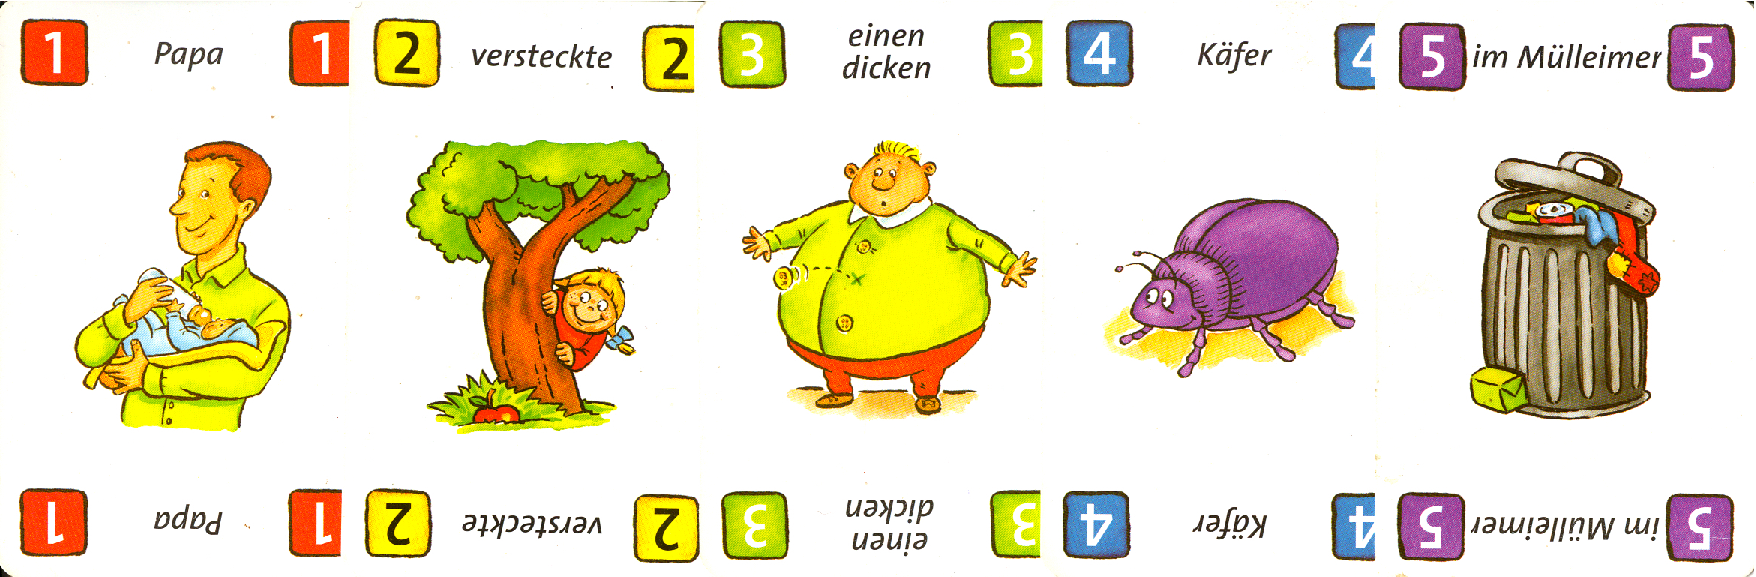
\includegraphics[width=\textwidth]{Bilder/lach-dich-schlapp-pappa-versteckte}

\vfill
Reihe die Spielkarten in der Reihenfolge 1 bis 5 aneinander.

\vfill
\footnotesize{(Ravensburger, 6--12 Jahre)}

}
\frame{
\frametitle{Lach Dich schlapp!}

\vfill
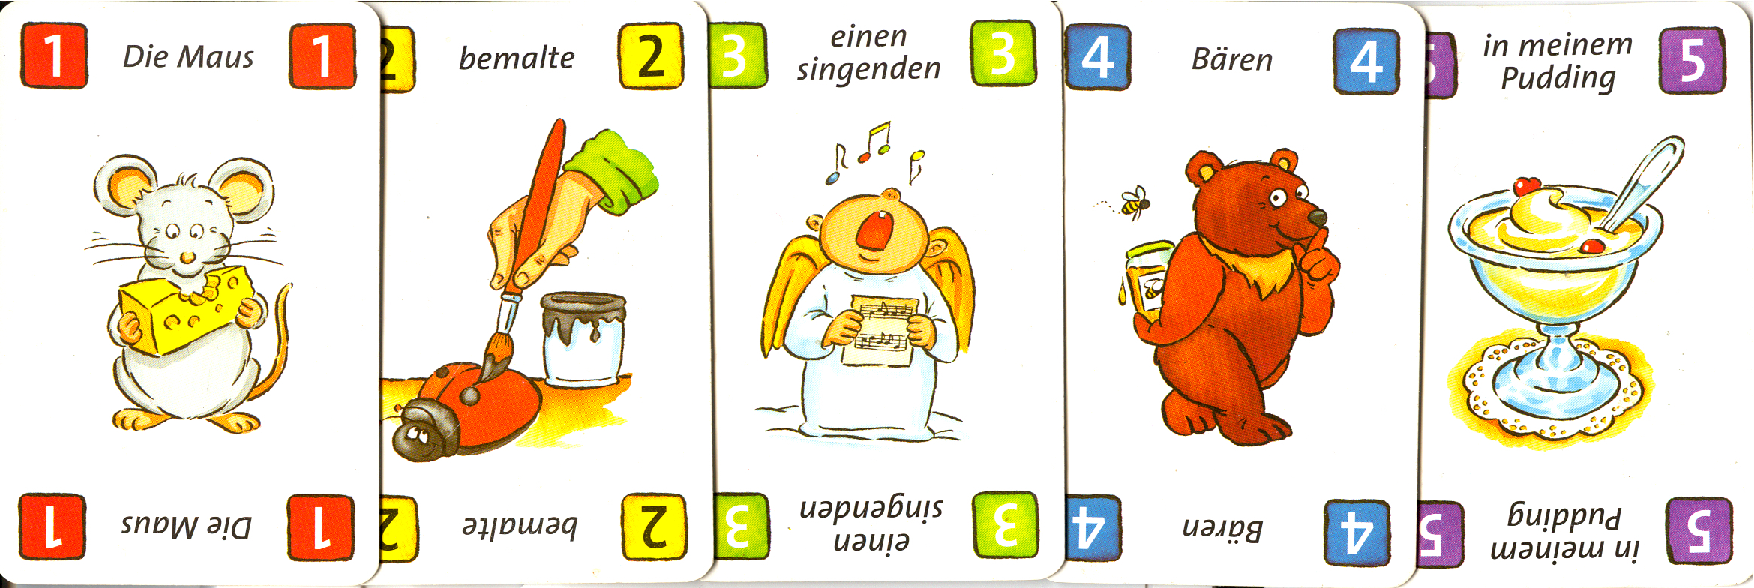
\includegraphics[width=\textwidth]{Bilder/lach-dich-schlapp-die-maus-bemalte}

\vfill
Warum funktioniert das Spiel?

\vfill
}


\frame{
\frametitle{Form und Bedeutung}


\begin{tabular}{@{}llll@{}}
{}[Papa]     & [versteckte] & [einen dicken Käfer]    & [im Mülleimer].\\
{}[Die Maus] & [bemalte]    & [einen singenden Bären] & [in meinem Pudding].
\end{tabular}

\bigskip

\begin{itemize}
\item Wir können die Blöcke austauschen und die Sätze bleiben wohlgeformt.

\item Allerdings passt die Bedeutung im zweiten Beispiel nicht mehr.

\pause

\item Zusammensetzung von Einheiten und Umordnung = \blaubf{Syntax}

\pause

\item Bedeutung im engeren und weiteren Sinn = \blaubf{Semantik}/\blaubf{Pragmatik}

\end{itemize}

}

%% \frame{
%% \frametitle{Verschwende Deine Jugend!}

%% \vfill
%% \centerline{\includegraphics[width=0.8\textwidth]{Bilder/daf}}

%% \vfill
%% }


%% \frame{
%% \frametitle{Spiel und Spaß}


%% Als kleiner Junge war mir schon klar: mein Leben wird ganz wunderbar.\\
%% Ich lebe einfach  radikal, nach Algorithmen meiner Wahl.\\
%% Ich richt' mein Leben radikal, nach Algorithmen meiner Wahl.\\
%% Ein Algorithmus ist ein Ball, darin gefangen eine Zahl.\\
%% Befrei die Zahl und spiel den Ball. Spiel den Ball.

%% D.A.F.: Fünfzehn neue DAF-Lieder, Superstar Recordings, 2003

%% \bigskip

%% Syntax = Spiel\\
%% Semantik = Spaß



%% }

}


\frame{
\frametitle{Syntax: Material}

\begin{itemize}
\item Müller, 2013. Grammatiktheorie. Tübingen: Stauffenburg-Verlag, Kapitel~1--2.\nocite{MuellerGTBuch2}


\url{https://www.researchgate.net/publication/258328909_Grammatiktheorie}

\pause
\item Oder auf Englisch: \url{http://langsci-press.org/catalog/book/25}


\bigskip

Zur Vorbereitung bitte immer entsprechende Abschnitte lesen! 

%\pause

%\item Im Sprachbeschreibungsteil werden wir \citew{Duden2009a} verwenden.
\end{itemize}

}

\exewidth{(370)}






\iftoggle{syntaxvorlesungen}{

\frame{
\frametitle{Alte Weisheit}

{}[Grammatik ist] das Tor zur Freiheit, die Medizin für die Krankheiten der Sprache, der Reiniger
aller Wissenschaften; sie verbreitet ihr Licht über ihnen; \ldots sie ist
die erste Sprosse auf der Leiter, die zur Realisierung übernatürlicher Kräfte führt und der
gerade, königliche Weg für diejenigen, die die Freiheit suchen. (Bhartrhari, Spruchdichter,
gest.\ vor 650 n. Chr., aus \emph{Vakyapadiya}, gefunden von Gabriele Knoll)

}
}

%\if 0

\iftoggle{einfsprachwiss-exclude}{
\section{Einleitung}
}

\iftoggle{hpsgvorlesung}{
\outline{

\begin{itemize}
\item Wozu Syntax? / Phrasenstrukturgrammatiken
\item Formalismus
\item Valenz und Grammatikregeln
\item Komplementation
\item Semantik
\item Adjunktion und Spezifikation
\item Das Lexikon: Typen und Lexikonregeln
\item Topologie des deutschen Satzes
\item Konstituentenreihenfolge
\item Nichtlokale Abhängigkeiten
\item Relativsätze
\item Lokalität
%\item Komplexe Prädikate: Der Verbalkomplex
\end{itemize}
}
}%\end{hpsgvorlesung}


\iftoggle{einfsprachwiss-exclude}{
\frame{
\frametitlefit{Motivation fromale Syntax und Phrasenstrukturgrammatiken}

\begin{itemize}
\item Literatur: \citew[Kapitel~1]{MuellerLehrbuch3} bzw.\ \citew[Kapitel~1]{MuellerGTBuch2}
\item Englische Version des Grammatiktheoriebuches: \citew{MuellerGT-Eng1}
\end{itemize}

\vspace{1cm}

%%\rotbf{Achtung, wichtiger Hinweis: Diese Literaturangabe hier bedeutet,\\dass Sie die Literatur zum
%%   nächsten Mal lesen sollen!!!!}
%% }
}
}%\end{einfsprachwiss-exclude}


\subsection{Wozu Syntax?}



\frame{
\frametitle{Wozu Syntax?}

\begin{itemize}
\item Literatur: \citew[Kapitel~1]{MuellerLehrbuch3} bzw.\ \citew[Kapitel~1]{MuellerGTBuch2}
\medskip

\item Zeichen: Form-Bedeutungs-Paare \citep{Saussure16a}
\pause
\item Wörter, Wortgruppen, Sätze
\pause
\item Sprache $\stackrel{?}{=}$ endliche Aufzählung von Wortfolgen\\
\pause
      Sprache ist endlich, wenn man maximale Satzlänge annimmt
      \eal
      \ex Dieser Satz geht weiter und weiter und weiter und weiter \ldots
\pause
      \ex {}[Ein Satz ist ein Satz] ist ein Satz.
      \zl
\pause
      extrem viele Sätze, Beschränkung der Wiederholung willkürlich

\item Unterscheidung zwischen \alert{Kompetenz} (das Wissen darüber, was geht) und
  \alert{Performanz} (der Benutzung des Wissens)

\end{itemize}
}


\frame{
\frametitle{Die Kinder von Bullerbü}

Und wir beeilten uns, den Jungen zu erzählen, wir hätten von Anfang an gewußt, daß es nur eine
Erfindung von Lasse gewesen sei. Und da sagte Lasse, die Jungen hätten gewußt, daß wir gewußt
hätten, es sei nur eine Erfindung von ihm. Das war natürlich gelogen, aber vorsichtshalber sagten
wir, wir hätten gewußt, die Jungen hätten gewußt, daß wir gewußt hätten, es sei nur eine Erfindung
von Lasse. Und da sagten die Jungen -- ja -- jetzt schaffe ich es nicht mehr aufzuzählen, aber es
waren so viele "`gewußt"', daß man ganz verwirrt davon werden konnte, wenn man es hörte. (S.\,248)

\bigskip

Wir sind prinzipiell in der Lage, komplexere Sätze zu bilden (Kompetenz), aber irgendwann werden wir
verwirrt, weil unsere Gehirne nicht mehr mitmachen (Performanz).


}




\frame{
\frametitle{Kreativität}


\begin{itemize}
\item Wir können Sätze bilden, die wir noch nie gehört haben $\to$\\
      muss Strukturierung, Muster geben

\end{itemize}


}

\frame{
\frametitle{Direkte Evidenz für syntaktische Strukturen?}

\begin{itemize}
\item Wir können feststellen, dass wir Regeln verwenden,\\
      indem wir Kinder beobachten.
      
      Kinder wenden Regeln mitunter falsch an (bzw. eben ihre eigenen Regeln).

\pause
\item Beispiel aus der Morphologie:
\eal
\ex[*]{
die Baggers
}
\ex[*]{
die Ritters
}
\zl
\end{itemize}
}


\frame{
\frametitle{Wozu Syntax? Bedeutung aus Bestandteilen ermitteln}

\begin{itemize}
\item Bedeutung einer Äußerung aus den Bedeutungen ihrer Teile bestimmen
      \ea
      Der Mann kennt diese Frau.
      \z
\pause
\item Syntax: Art und Weise der Kombination, Strukturierung 
      \eal
      \ex Die Frau kennt die Mädchen.
      \ex Die Frau kennen die Mädchen.
\pause
      \ex Die Frau schläft.
      \ex Die Mädchen schlafen.
      \zl
        Subjekt-Verb-Kongruenz $\to$ Bedeutung von (\mex{0}a,b) ist eindeutig
\end{itemize}

}

\subsection{Warum formal?}
\frame[shrink=20]{
\frametitle{Warum formal?}


Precisely constructed models for linguistic structure can play an
important role, both negative and positive, in the process of discovery 
itself. By pushing a precise but inadequate formulation to
an unacceptable conclusion, we can often expose the exact source
of this inadequacy and, consequently, gain a deeper understanding
of the linguistic data. More positively, a formalized theory may 
automatically provide solutions for many problems other than those
for which it was explicitly designed. Obscure and intuition-bound
notions can neither lead to absurd conclusions nor provide new and
correct ones, and hence they fail to be useful in two important respects. 
I think that some of those linguists who have questioned
the value of precise and technical development of linguistic theory
have failed to recognize the productive potential in the method
of rigorously stating a proposed theory and applying it strictly to
linguistic material with no attempt to avoid unacceptable conclusions by ad hoc adjustments or loose formulation.
\citep[S.\,5]{Chomsky57a}


As is frequently pointed out but cannot be overemphasized, an important goal
of formalization in linguistics is to enable subsequent researchers to see the defects
of an analysis as clearly as its merits; only then can progress be made efficiently.
\citep[S.\,322]{Dowty79a}


\bigskip

\begin{itemize}
\item Was bedeutet eine Analyse genau?
\item Welche Vorhersagen macht sie?
\item Ausschluß anderer Analysen
\end{itemize}


}

% has to be set elsewhere since this file is included into the syntax vorlesung
%\exewidth{(35)}

\subsection{Konstituenz}

\subsubsection{Konstituententests}

\frame{
\frametitle{Einteilung in Einheiten}

\begin{itemize}
\item Sätze können Sätze enthalten, die Sätze enthalten, die \ldots:
\ea
dass Max glaubt, [dass Julius weiß, [dass Otto behauptet, [dass Karl vermutet, [dass Richard bestätigt,
[dass Friederike lacht]]]]]
\z

Das funktioniert wie eine Matrjoschka bzw.\ wie eine Zwiebel.

\pause

\item Genauso kann man in (\mex{1}) Wörter zu Einheiten zusammenfassen:
\ea
Alle Studenten lesen während dieser Zeit Bücher.
\z

Welche?

\end{itemize}


}

\frame{
\frametitle{Schachteln}

\oneline{%
\begin{pspicture}(0,0)(12,1.8)
     \rput[bl](0,0){%
\psset{fillstyle=solid, framearc=0.25,framesep=5pt}
\psframebox{%
\psframebox{%
       \psframebox{alle}
       \psframebox{Studenten}}
\psframebox{lesen}
\psframebox{%
       \psframebox{während}
       \psframebox{%
           \psframebox{dieser}
           \psframebox{Zeit}}}
\psframebox{Bücher}}}
%\psgrid
    \end{pspicture}}

Wir tun alle Wörter, die zusammengehören, in eine Schachtel. 

Diese Schachteln können wieder in andere Schachteln getan werden.

Im Beispiel ist intuitiv klar, was zusammengehört, aber gibt es Tests?

}


\frame{
\frametitle{Konstituenz}

Begriffe:
\begin{description}
\item[Wortfolge]  Eine beliebige linear zusammenhängende Folge von Wörtern,\\
                  die nicht unbedingt syntaktisch oder semantisch zusammengehörig sein müssen.
\item[Wortgruppe, Konstituente, Phrase] Ein Wort oder mehrere Wörter,\\
                  die eine strukturelle Einheit bilden.
\end{description}


}

\iftoggle{syntaxvorlesungen}{
\frame{
\frametitle{Konstituententests}

Welche kennen Sie?
\pause

\begin{itemize}
\item Substituierbarkeit/Pronominalisierungstest/Fragetest
\item Weglaßtest
\item Verschiebetest (Umstelltest)
\item Koordinationstest
\end{itemize}


}
}%\end{syntaxvorlesungen}


\frame{
\frametitle{Konstituententests (I)}


\begin{description}
\item[Substituierbarkeit]
        Kann man eine Wortfolge einer bestimmten
	Kategorie in einem Satz gegen eine andere Wortfolge so austauschen, dass
	wieder ein akzeptabler Satz entsteht, so ist das ein Indiz dafür, dass 
	die beiden Wortfolgen Konstituenten bilden.
        \eal
        \ex Er kennt den Mann.
        \ex Er kennt eine Frau.
        \zl
\pause
\item[Pronominalisierungstest]
        Alles, worauf man sich mit einem Pronomen beziehen
	kann, ist eine Konstituente.
        \eal
        \ex Der Mann schläft.
        \ex Er schläft.
        \zl
%
\end{description}

}

\frame{
\frametitle{Konstituententests (II)}

\begin{description}
\item[Fragetest]
        Was sich erfragen läßt, ist eine Konstituente.
        \eal
        \ex Der Mann arbeitet.
        \ex Wer arbeitet?
        \zl
\pause
\item[Verschiebetest] Wortfolgen, die man ohne Beeinträchtigung der
	Korrektheit des Satzes verschieben bzw.\ umstellen kann, bilden eine Konstituente.
        \eal
        \ex weil keiner diese Frau kennt.
        \ex weil diese Frau keiner kennt.
        \zl
\pause
\item[Koordinationstest]
        Was sich koordinieren läßt, ist eine Konstituente.
        \ea
        Der Mann und die Frau arbeiten.
        \z
\end{description}

}



\iftoggle{konstituentenprobleme}{
\subsubsection{Bemerkungen zum Status der Tests}

\frame{
\frametitle{Bemerkungen zum Status der Tests: Expletiva (I)}

Was ist mit \emph{es} in (\mex{1})?
\ea
Es regnet.
\z
\pause

Substituierbarkeit und Fragetest schlagen fehl:
\eal
\ex[*]{
Der Mann/er regnet.
}
\ex[*]{
Wer/was regent?
}
\zl
Aus denselben Gründen schlägt der Koordinationstest fehl:
\ea[*]{
Es und der Mann regnet.
}
\z

}


\frame{
\frametitle{Bemerkungen zum Status der Tests: Expletiva (II)}

Nur die (allerdings eingeschränkte) Umstellbarkeit ist gegeben:
\eal
\ex[]{
Es regnet.
}
\ex[]{
Regnet es?
}
\ex[]{
weil es jetzt regnet
}
\ex[*]{
weil jetzt es regnet
}
\zl
\eal
\ex[]{
Er sah es regnen.
}
\ex[*]{
Es sah er regnen.
}
\zl

\pause
Daraus folgt: Nicht alle Tests müssen positiv ausfallen,\\
damit eine Wortfolge als Konstituente gelten kann,\\
\dash, die Test stellen keine notwendige Bedingung dar.


}


\frame[shrink=10]{
\frametitle{Bemerkungen zum Status der Tests: Koordination}

%\judgewidth{?*}
\smallframe
Was ist mit \emph{der Mann einen Esel} und \emph{die Frau ein Pferd} in (\mex{1})?
\ea
Deshalb kaufte der Mann einen Esel und die Frau ein Pferd.
\z
\pause

Diese Wörter kann man nur sehr bedingt gemeinsam umstellen:
\ea[?*]{
Der Mann einen Esel kaufte deshalb.
}
\z

Ein Ersetzung durch Pronomina ist nicht ohne Ellipse möglich:
\eal
\ex[\#]{
Deshalb kaufte er.
}
\ex[*]{
Deshalb kaufte ihn.
}
\zl
Die Pronomina stehen nicht für beide logischen Argumente % von \emph{kaufen},
sondern nur für jeweils eins.

\pause
Daraus folgt: Auch wenn einige Tests erfüllt sind,\\
muß es noch lange nicht sinnvoll sein, eine Wortfolge als Konstituente einzustufen,\\
\dash, die Test stellen keine hinreichende Bedingung dar.

}

\frame{
\frametitle{Bemerkungen zum Status der Tests: Voranstellung (I)}
%
\savespace\smallexamples

Normalerweise steht im Deutschen eine Konstituente vor dem Finitum.

{\judgewidth{?*}
\eal
\ex[]{
[Alle Studenten] lesen während der vorlesungsfreien Zeit Bücher.
}
\ex[]{
[Bücher] lesen alle Studenten während der vorlesungsfreien Zeit.
}
\ex[*]{
[Alle Studenten] [Bücher] lesen während der vorlesungsfreien Zeit.
}
\ex[*]{
[Bücher] [alle Studenten] lesen während der vorlesungsfreien Zeit.
}
\zl
}

Voranstellbarkeit vor das finite Verb wird in manchen Definitionen sogar
zum ausschlaggebenden Kriterium für \textit{Satzglied} \citep[S.\,783]{Duden2005}.
}

\frame{
\frametitle{Bemerkungen zum Status der Tests: Voranstellung (II)}

%\begin{tabular}{@{p{0.95\linewidth}}
\alert{Satzgliedtest} [Auch: Konsituententest]. Auf der $\to$ Topikalisierung
beruhendes Verfahren zur Analyse komplexer Konstituenten. Da bei Topikalisierung
jeweils nur eine Konstituente bzw.\ ein $\to$ Satzglied an den Anfang gerückt werden kann,
lassen sich komplexe Abfolgen von Konstituenten (\zb Adverbialphrasen) als
ein oder mehrere Satzglieder ausweisen; in \textit{Ein Taxi quält sich im Schrittempo
durch den Verkehr} sind \textit{im Schrittempo} und \textit{durch den Verkehr}
zwei Satzglieder, da sie beide unabhängig voneinander in Anfangsposition gerückt werden
können. \citep[S.\,446]{Bussmann83a}
%\end{tabular}

\bigskip
nicht mehr enthalten in \citew{Bussmann90a}

}

\frame{
\frametitle{Bemerkungen zum Status der Tests: Voranstellung (III)}


Nach Bußmann:
\begin{itemize}
\item Teile des Materials können einzeln vorangestellt werden. $\to$\\
      Das Material bildet keine Konstituente.
\item Material kann zusammen vorangestellt werden. $\to$\\
      Das Material bildet eine Konstituente.
\end{itemize}

Beide Implikationen sind problematisch.

Die erste ist wegen Beispielen wie (\mex{1}) problematisch:
\eal
\ex \rot{Keine Einigung} \blau{erreichten} Schröder und Chirac \gruen{über den Abbau der Agrarsubventionen}. (tagesschau, 15.10.2002, 20:00)
\ex \gruen{Über den Abbau der Agrarsubventionen} \blau{erreichten} Schröder und Chirac \rot{keine Einigung}.
\zl

}

\frame{
\frametitle{Bemerkungen zum Status der Tests: Voranstellung (IV)}

Obwohl Teile der NP einzeln vorangestellt werden können,
wollen wir die Wortfolge als eine NP analysieren, wenn sie nicht vorangestellt ist.
\ea
Schröder und Chirac \blau{erreichten} \rot{keine Einigung} \gruen{über den Abbau der Agrarsubventionen}.
\z
\pause
Diese Wortgruppe kann auch gemeinsam vorangestellt werden:
\ea
\rot{Keine Einigung} \gruen{über den Abbau der Agrarsubventionen} \blau{erreichten} Schröder und Chirac.
\z

\emph{Keine Einigung über den Abbau der Agrarsubventionen} ist eine Konstituente, 
die unter gewissen Umständen aufgespalten werden kann. 

Bei Aufspaltung können die einzelnen Teilkonstituenten unabhängig voneinander umgestellt werden.

}

\frame{
\frametitle{Bemerkungen zum Status der Tests: Voranstellung (V)}

\small
\savespace
\smallexamples
Der zweite Teil des Konstituententests ist ebenfalls problematisch:


\eal
\ex {}[Dauerhaft] [mehr Arbeitsplätze] gebe es erst, wenn sich eine Wachstumsrate von
      mindestens 2,5 Prozent über einen Zeitraum von drei oder vier Jahren halten lasse. (taz, 19.04.2000, S.\,5)
\ex {}[Wenig] [mit Sprachgeschichte] hat der dritte Beitrag in dieser Rubrik zu tun, [\ldots]
    (ZS für Dialektologie und Linguistik, LXIX, 3/2002, S.\,339)
\zl


Mehr Daten in \citew{Mueller2003b}.

Wörter vor Finitum stehen werder in semantischer noch in syntaktischer Beziehung zueinander
$\to$ nicht sinnvoll, sie als eine Konstituente zu analysieren

\medskip
Die Daten kann man mit einem leeren verbalen Kopf im Vorfeld analysieren,\\
so dass letztendlich wieder V2-Strukturen vorliegen \citep{Mueller2005d}.\\
Trotzdem sind die Daten für Konstituententests problematisch.

Voranstellbarkeit ist nicht hinreichend für Konstituentenstatus.

}

\frame{
\frametitle{Bemerkungen zum Status der Tests: Voranstellung (VI)}

\judgewidth{\#}
\eal
\ex[]{
Er bringt es bis zum Professor.
}
\ex[\#]{
Es bringt er zum Professor.
} 
\zl

\emph{es} ist Konstituente, obwohl es nicht vorangestellt werden kann.

\pause
Genauso:
\eal
\ex[]{
Karl hat sich nicht erholt.
}
\ex[*]{
Sich hat Karl nicht erholt.
}
\zl

\eal
\ex[]{
Er hörte es regnen.
}
\ex[*]{
Es hörte er regnen.
}
\zl

$\to$ Voranstellbarkeit ist nicht notwendig.

Also: Voranstellbarkeit ist weder hinreichend noch notwendig.

}
}%\end{konstituentenprobleme}


\iftoggle{konstituentenprobleme-hinweis}{

\frame{
\frametitle{Warnung}


Achtung: Diese Tests liefern leider nur Indizien für den Konstituentenstatus. 

Zu den Details siehe 
%\citew[Kapitel~1.3.2]{MuellerLehrbuch3}
\citew[Kapitel~1.3.2]{MuellerGTBuch2}.
}

}%\end{konstituentenprobleme-hinweis}

\subsection{Köpfe}



\frame{
\frametitle{Köpfe}

Kopf bestimmt die wichtigsten Eigenschaften einer Phrase
\eal
\ex \alert{Träumt} er?
\ex \alert{Erwartet} er einen dreiprozentigen Anstieg?
\ex \alert{in} diesem Haus
\ex ein \alert{Mann}
\zl

\pause
Kombination eines Kopfes mit anderem Material wird
\alert{Projektion des Kopfes} genannt.

\pause
Eine vollständige Projektion ist eine \alert{Maximalprojektion}.

\pause
Ein Satz ist die Maximalprojektion eines finiten Verbs.
}

\frame{
\frametitle{Beschriftete Schachteln}

\medskip

\centerline{%
\begin{pspicture}(0,0)(7.8,3.4)
     \rput[bl](0,0){%
\psset{fillstyle=solid, framearc=0.25,framesep=5pt}
\psframebox{%
\begin{tabular}{@{}l@{}}
VP\\
\psframebox{%
\begin{tabular}{@{}l@{}}
NP\\[2mm]
       \psframebox{\begin{tabular}{@{}l@{}}
                   Det\\der
                   \end{tabular}}
       \psframebox{\begin{tabular}{@{}l@{}}
                   N\\Mann
                   \end{tabular}}
\end{tabular}}
\psframebox{\begin{tabular}{@{}l@{}}
                   V\\liest
                   \end{tabular}}
\psframebox{%
\begin{tabular}{@{}l@{}}
NP\\[2mm]
           \psframebox{\begin{tabular}{@{}l@{}}
                   Det\\einen
                   \end{tabular}}
           \psframebox{\begin{tabular}{@{}l@{}}
                   N\\Aufsatz
                   \end{tabular}}
\end{tabular}}
\end{tabular}}}
%\psgrid
    \end{pspicture}}


Wer schon einmal umgezogen ist, weiß, dass es sinnvoll ist,\\
Schachteln zu beschriften.

Im obigen Bild steht auf jeder Schachtel etwas über das wichtigste Element in der Schachtel.

}

\frame[shrink=15]{
\frametitle{Schachteln sind austauschbar}


\begin{itemize}
\item Der genaue Inhalt einer Schachtel ist egal:
\eal
\ex er
\ex der Mann
\ex der Mann aus Stuttgart
\ex der Mann aus Stuttgart, den wir kennen
\zl
Wichtig ist: Die Wörter bzw.\ Wortfolgen in (\mex{0}) sind alle nominal und vollständig: NP.

Man kann sie innerhalb größerer Schachtel gegeneinander vertauschen.

\pause
\item Das geht aber nicht mit allen NPen:

\eal
\ex[]{ 
Der Mann liest einen Aufsatz.  
} 
\ex[*]{ 
Die Männer liest einen Aufsatz.  
} 
\ex[*]{ Des Mannes liest einen Aufsatz.  
} 
\zl 

\item Es gibt Eigenschaften, die für die Verteilung (Distribution) von Phrasen wichtig sind.


\end{itemize}


}

\frame{
\frametitle{Ausführlich beschriftete Schachteln}

~\medskip

\oneline{%
\begin{pspicture}(0,0)(16.4,3.4)
     \rput[bl](0,0){%
\psset{fillstyle=solid, framearc=0.25,framesep=5pt}
\psframebox{%
\begin{tabular}{@{}l@{}}
VP, fin\\[2mm]
\psframebox{%
\begin{tabular}{@{}l@{}}
NP, nom, 3, sg, mas\\[2mm]
       \psframebox{\begin{tabular}{@{}l@{}}
                   Det, nom, sg, mas\\der
                   \end{tabular}}
       \psframebox{\begin{tabular}{@{}l@{}}
                   N, nom, sg, mas\\Mann
                   \end{tabular}}
\end{tabular}}
\psframebox{\begin{tabular}{@{}l@{}}
                   V, fin, 3, sg\\liest
                   \end{tabular}}
\psframebox{%
\begin{tabular}{@{}l@{}}
NP, akk, 3, sg, mas\\[2mm]
           \psframebox{\begin{tabular}{@{}l@{}}
                   Det, akk, sg, mas\\einen
                   \end{tabular}}
           \psframebox{\begin{tabular}{@{}l@{}}
                   N, akk, sg, mas\\Aufsatz
                   \end{tabular}}
\end{tabular}}
\end{tabular}}}
%\psgrid
    \end{pspicture}}

Alle Merkmale, die für die Distribution der gesamten Phrase wichtig sind, werden projiziert.

Diese Merkmale werden auch \alert{Kopfmerkmale} genannt.

}


% \frame[shrink=10]{
% \frametitle{Projizierte Merkmale}


% \hfill%
% \begin{tabular}{|l|l|}\hline
% Kategorie    & projizierte Merkmale\\\hline
% Verb         & Kategorie, Verbform ({\it fin\/}, {\it bse\/}, \ldots)\\
% Nomen        & Kategorie, Kasus ({\it nom\/}, {\it gen\/}, {\it dat\/}, {\it acc\/})\\
% %Präposition  & Kategorie, Form der Präposition ({\it an\/}, {\it auf\/}, \ldots)\\
% Adjektiv     & Kategorie, bei flektierten Formen Kasus\\\hline
% \end{tabular}\hfill\hfill\mbox{}
% \pause
% ~
% \bigskip

% Beispiel:
% Wenn \emph{stolzer} den Kasus Genitiv hat,\\
% dann hat auch die gesamte Adjektiv-Phrase Genitiv. 

% \ea
% \emph<3>{einiger \emph<2>{auf ihren Sohn \blau<2>{stolzer}} \blau<3>{Männer}}
% \z

% Das ist wichtig, da die Adjektiv-Phrase mit dem Determinierer und\\
% dem Nomen im Kasus übereinstimmen muß.

% \pause
% Wenn \emph{Männern} in (\mex{1}) Dativ ist, hat die gesamte NP diese Eigenschaft.
% \ea
% den Männern
% \z

% }

%\fi

\subsection{Argumente und Adjunkte}

\frame[shrink=10]{
\frametitle{Argumente}

\begin{itemize}
\item Konstituenten stehen in verschiedenartigen Beziehungen zu ihrem Kopf.
\pause
\item Man unterscheidet zwischen \alert{Argumenten} und \alert{Adjunkten}.
\pause
\item Bestimmte Mitspieler (Aktanten) gehören zur Bedeutung eines Verbs.

\ZB gibt es in Situationen, die durch \emph{lieben} beschrieben werden,\\
immer einen \emph{Liebenden} und einen \emph{Geliebten} / etwas \emph{Geliebtes}.

\eal
\ex Peter liebt Maria.
\ex $lieben'(Peter', Maria')$
\zl

(\mex{0}b) ist eine logische Repräsentation für (\mex{0}a).

\relation{Peter} und \relation{Maria} sind \alert{logische Argumente} von \relation{lieben}.

\pause
\item Syntaktische Argumente entsprechen meistens den logischen (später mehr).
\pause
\item Solche Beziehungen zwischen Kopf und Argumenten werden mit dem Begriff
\alert{Selektion} bzw.\ \alert{Valenz} erfasst.
\pause
\item \citet{Tesniere59a-u} überträgt Valenzbegriff aus der Chemie auf die Linguistik.
\end{itemize}

}


%\BackgroundPicture{periodensystem}{1}{1}
\frame{
\frametitle{Valenz in der Chemie}

\begin{itemize}
\item Atome können sich mit anderen Atomen zu mehr oder weniger stabilen Molekülen verbinden. 

\pause
\item Wichtig für die Stabilität ist, wie Elektronenschalen besetzt sind. 

\pause
\item Eine Verbindung mit anderen Atomen kann dazu führen,\\
dass eine Elektronenschale voll besetzt ist,\\
was dann zu einer stabilen Verbindung führt.

\pause
\item Die Valenz sagt etwas über die Anzahl der Wasserstoffatome aus,\\
die mit einem Atom eines Elements verbunden werden können. 

\pause
\item Sauerstoff hat die Valenz 2 und kann sich zu H$_2$O verbinden.

\pause
\item Man kann nun die Elemente in Valenzklassen einteilen.\\
Elemente mit einer bestimmten Valenz werden im Periodensystem von Mendeleev
in einer Spalte repräsentiert.

\end{itemize}

}

\frame{
\frametitle{Valenz in der Linguistik}

\begin{itemize}
\item Ein Kopf braucht bestimmte Argumente,\\
      um eine stabile Verbindung einzugehen. 
\item Wörter mit der gleichen Valenz (mit gleicher Anzahl und Art von Argumenten)  werden in Valenzklassen eingeordnet, da sie sich in bezug
auf die Verbindungen, die sie eingehen, gleich verhalten. 


\bigskip

\centerline{
\begin{forest}
[O
  [H] 
  [H] ]
\end{forest}
\hspace{5em}
\begin{forest}
[helfen
 [Peter]
 [Maria] ]
\end{forest}
}

\bigskip

Verbindung von Sauerstoff mit Wasserstoff und Verbindung
eines Verbs mit seinen Argumenten

\end{itemize}

\vfill

}

\frame{
\frametitle{Optionale Argumente}

\begin{itemize}
\item Argumente müssen nicht immer realisiert werden:
\eal
\ex Er wartet auf den Installateur.
\ex Er wartet.
\zl
\pause
Das Präpositionalobjekt von \emph{warten} 
ist ein \alert{fakultatives Argument}.

\pause
\item In nominalen Umgebungen sind Argumente immer optional!
\eal
\ex Jemand liest diese Bücher.
\ex das Lesen dieser Bücher
\ex das Lesen
\zl

\end{itemize}
}

\frame{
\frametitle{Syntaktische Argumente, die keine logischen sind}

\begin{itemize}
\item In unserem bisherigen Beispiel entsprechen die syntaktischen den logischen Argumenten:
\eal
\ex Peter liebt Maria.
\ex $lieben'(Peter', Maria')$
\zl

\pause
\item Allerdings gibt es auch Argumente, die keinen semantischen Beitrag leisten:

\eal
\ex Es regnet.
\ex Peter erholt sich.
\zl
\emph{es} und \emph{sich} sind \alert{syntaktische Argumente},\\
aber keine \alert{logischen Argumente}.

\end{itemize}
}

\frame{
\frametitle{Argumente und Adjunkte}


\begin{itemize}
\item Adjunkte füllen keine semantische Rolle
\item Adjunkte sind optional
\item Adjunkte sind iterierbar
\end{itemize}


}


\frame{
\frametitle{Adjunkte füllen keine semantische Rolle}

\begin{itemize}
\item In einer \emph{lieben}"=Situation gibt es einen Liebenden und etwas Geliebtes.

\emph{seit der Schulzeit} in (\mex{1}) ist von anderer Art:
\ea
Peter liebt Maria seit der Schulzeit.
\z
Es sagt zusätzlich etwas über die Dauer der Relation aus,\\
in der Peter und Maria zueinander stehen.

\end{itemize}

}

\frame{
\frametitle{Adjunkte sind optional}


\begin{itemize}
\item Adjunkte sind optional:
\eal
\ex Peter liebt Maria.
\ex Peter liebt Maria seit der Schulzeit.
\ex Peter liebt Maria aufrichtig.
\zl
\pause
\item Vorsicht! Das ist auch bei Argumenten mitunter der Fall:
\eal
\ex Er gibt den Armen Geld.
\ex Er gibt den Armen.
\pause
\ex Er gibt Geld.
\pause
\ex Er gibt gerne.
\pause
\ex Du gibst. (beim Skat)
\pause
\ex Gib!
\zl
\end{itemize}


}



\frame{
\frametitle{Adjunkte sind iterierbar}


\begin{itemize}
\item Argumente können nur einmal mit dem Kopf kombiniert werden:
\ea[*]{
Der Mann der Mann schläft.
}
\z

Die entsprechende Andockstelle des Kopfes (\emph{schläft}) ist besetzt.

\pause
\item Bei Adjunkten ist das anders:

\ea
\label{Beispiel-Iteration-Adjektive}
A: Alle klugen Frauen sind unglücklich.\\
B: Nein, ich kenne eine glückliche kluge Frau.\\
A: Aber alle glücklichen klugen Frauen sind schön.\\
B: Nein, ich kenne eine hässliche glückliche kluge Frau.\\
\hspaceThis{A:~}\ldots
\z

\end{itemize}

}

\frame{
\frametitle{Weiter Beispiele für Adjunkte}


Adverbial gebrauchtes Adjektiv (nicht alle Adjektive):
\ea
Karl schnarcht \emph{laut}.
\z


Relativsätze (nicht alle):
\eal
\ex der Mann, \emph{den Maria liebt}
\ex der Mann, \emph{der Maria liebt}
\zl


Präpositionalphrasen (nicht alle):
\eal
\ex Die Frau arbeitet \emph{in Berlin}.
\ex die Frau \emph{aus Berlin}
\zl



}

%\if 0



\frame{
\frametitle{Andere Bezeichnungen}

\begin{itemize}
\item Argument: Ergänzung

\pause
\item Adjunkt: (freie) Angabe

\pause
\item Argumente werden mitunter in Subjekt und Komplemente aufgeteilt.

\pause
\item auch Aktant für Subjekte und Objekte\\
      (aber nicht Prädikative und Adverbialien)
\pause
\item Zirkumstant für Adverbialien
      \begin{itemize}
      \item Adverbiale des Raumes (Lage, Richtung/Ziel, Herkunft, Weg)
      \item Adverbiale der Zeit (Zeitpunkt, Anfang, Ende, Dauer)
      \item Adverbiale des Grundes.\\
            Hierher werden traditionellerweise auch Adverbialien gestellt,\\
                   die einen Gegengrund oder eine Bedingung ausdrücken.
      \item Adverbiale der Art und Weise. 
      \end{itemize}
\end{itemize}

}


\iftoggle{einfsprachwiss-include}{

\subsection{Grammatische Funktionen}


\subsubsection{Subjekt}

\frame{
\frametitle{Subjekt}

Definition ist nicht trivial.

Für das Deutsche wurden folgende syntaktische Eigenschaften von Subjekten genannt:
\begin{itemize}
\item Kongruenz mit dem finiten Verb
\item Nominativ in nichtkopulativen Sätzen
\item Weglassbarkeit in Infinitivkonstruktionen (Kontrolle)
\item Weglassbarkeit in Imperativsätzen
\end{itemize}

\citet{Reis82}: der zweite Punkt reicht für das Deutsche als Kriterium aus.

Einschränkung auf nichtkopulative Sätze:
\eal
\ex \blaubf{Er} ist ein Lügner.
\ex \blaubf{Er} wurde ein Lügner genannt.
\zl

}

\frame{
\frametitle{Dative sind keine Subjekte}

Kongruenz:
\eal
\ex[]{
Er hilft den Männern.
}
\ex[]{
Den Männern wurde geholfen.
}
\ex[*]{
Den Männern wurden geholfen.
}
\zl

\pause
Keine Kontrolle in Infinitivkonstruktionen:
\eal
\ex[]{
Klaus behauptet, den Männern zu helfen.
}
\ex[]{
Klaus behauptet, dass er den Männern hilft.
}
\pause
\ex[]{
Klaus behauptet, seine Familie zu lieben.
}
\ex[]{
Seine Familie behauptet, geliebt zu werden.
}
\pause
\ex[*]{
Die Männer behaupten, geholfen zu werden.
}
\ex[*]{
Die Männer behaupten, elegant getanzt zu werden.
}
\zl

}

\frame{
\frametitle{Dative sind keine Subjekte}

Weglassbarkeit in Imperativen:
\eal
\ex[]{
Fürchte dich nicht!
}
\ex[*]{
Graue nicht!
}
\ex[]{
Werd einmal unterstützt und \ldots
}
\ex[*]{
Werd einmal geholfen und \ldots
}
\zl

}


\subsubsection{Die Objekte}

\frame{
\frametitle{Die Objekte}

Im Deutschen gibt es Genitiv-, Dativ-, Akkusativ-, und Präpositionalobjekte: 
\eal
\ex Sie gedenken des Mannes.
\ex Sie helfen dem Mann.
\ex Sie kennen den Mann.
\ex Sie denken an den Mann.
\zl
}

\subsubsection{Das Adverbiale}

\frame{
\frametitle{Das Adverbiale}

Adverbialien sind oft Adverbien (daher die Bezeichnung).

Allerdings auch PP, NP, Sätze:
\eal
\ex Er arbeitet in der Universität.
\ex Er arbeitet den ganzen Tag.
\ex Er arbeitet, weil es ihm Spaß macht.
\zl

\emph{den ganzen Tag} ist kein Objekt, sondern adverbialer Akkusativ der Zeit. 

Solche Akkusative kommen mit Verben aus verschiedenen Valenzklassen vor:
\eal
\ex Er liest den ganzen Tag diesen schwierigen Aufsatz.
\ex Er gibt den Armen den ganzen Tag Suppe.
\zl

}


\frame{
\frametitle{Adverbialer Akkusativ der Zeit}

Bei Passivierung ändert sich der Kasus nicht:
\eal
\ex[]{
weil den ganzen Tag gearbeitet wurde
}
\ex[*]{
weil der ganze Tag gearbeitet wurde
}
\zl

Diese Akkusative sind so genannte \alert{semantische Kasus}.

}

\subsubsection{Das Prädikativ}

\frame{
\frametitle{Das Prädikativ}

\eal
\ex Klaus ist \blaubf{klug}.
\ex Er isst den Fisch \blaubf{roh}.
%\ex Er fährt das Auto kaputt.
\zl
\pause

\eal
\ex Sie nannte ihn \blaubf{einen Lügner}.
\ex Er wurde \blaubf{ein Lügner} genannt.
\zl

\pause
Zu weiteren Prädikativen siehe \citew{Duden2005}.

}

}%\end{einfsprachwiss-include}

\subsection[Grammatikmodelle]{Verschiedene Grammatikmodelle}

\frame{
\frametitle{Verschiedene Grammatikmodelle (I)}

\begin{itemize}
\item Dependenzgrammatik (DG)\\\citep{Tesniere80a-u,Tesniere2015a-u,Kunze75a-u,Weber97a,Heringer96a-u,Eroms2000a}
\item Kategorialgrammatik (CG)\\\citep{Ajdukiewicz35a-u,Steedman2000a-u}
\item Phrasenstrukturgrammatik (PSG)\nocite{Bloomfield33-u}
\item Transformationsgrammatik und deren Nachfolger
      \begin{itemize}
      \item Transformationsgrammatik \\\citep{Chomsky57a,Bierwisch63}
      \item Government \& Binding \\\citep{Chomsky81a,SS88a,Grewendorf88a}
      \item Minimalismus \\\citep{Chomsky95a-u,Grewendorf2002a}
      \end{itemize}
\end{itemize}


}
\frame{
\frametitle{Verschiedene Grammatikmodelle (II)}

\begin{itemize}
\item Tree Adjoning Grammar\\
      \citep*{JLT75a-u,Joshi87a-u,KJ85a}
\item Generalisierte Phrasenstrukturgrammatik (GPSG)\\\citep*{GKPS85a,Uszkoreit87a}
\item Lexikalisch Funktionale Grammatik (LFG)\\\citep{Bresnan82a-ed,Bresnan2001a,BF96a-u,Berman2003a}
\item Head-Driven Phrase Structure Grammar (HPSG)\\\citep{ps,ps2,Mueller99a,Mueller2002b,MuellerLehrbuch3}
\item Construction Grammar (CxG)\\\citep*{FKoC88a,Goldberg95a,Goldberg2006a,FS2006a-ed}

\bigskip
\item Zu einem Überblick siehe \citew{MuellerGTBuch1} bzw.\ \citew{MuellerGT-Eng1}.
\end{itemize}


}

%\input{hpsg-phrasenstrukturgrammatik}

%\fi



% \subsection{Transformationsgrammatik}
% \frame{
% \frametitle{Transformationsgrammatik}


% Im folgenden sehen wir uns eine Art Grammatik genauer an: die Transformationsgrammatik, oft auch als
% Generative Grammatik bezeichnet.

% Achtung: Es gibt auch andere generative Grammatiken, man sollte also vorsichtiger von \emph{Mainstream Generative
% Grammar} sprechen.





% }

\exewidth{(370)}
% ../../Grammatiktheorie/4a-gengram-tmodell.tex
% ../../Grammatiktheorie/4b-gengram-cpip.tex


%
\input formgram-xbar



\subsubsection{Verbalphrasen}


\frame[shrink=13]{
\frametitle{Verbalphrasen}

Adjunkte (freie Angaben) verbinden sich mit beliebigen V-Projektionen.

\ea
(dass) der Mann morgen den Jungen trifft
\z

\centerfit{
\begin{forest}
sn edges
[VP
  [NP [der Mann,triangle]]
  [V$'$ 
    [AdvP [morgen,triangle]]
    [V$'$ 
      [NP [den Jungen,triangle]]
      [V [trifft]]]]]
\end{forest}
}

}


\frame[shrink=20]{
\frametitle{Komplementiererphrasen}

Komplementierer verbinden sich mit Verbphrasen:

\centerfit{
\begin{forest}
sn edges
[CP
  [C$'$
    [C [dass]]
    [VP
      [NP [der Mann,triangle]]
      [V$'$ 
        [AdvP [morgen,triangle]]
        [V$'$ 
          [NP [den Jungen,triangle]]
          [V [trifft]]]]]]]
\end{forest}
}

}


%%%%%%%%%%%%%%%%%%%%%%%%%%%%%%%%%%%%%%%%%%%%%%%%%%%%%%%%%
%%   $RCSfile: 3-gengram-grundfragen.tex,v $
%%  $Revision: 1.1 $
%%      $Date: 2004/04/26 14:10:21 $
%%    Authors: Stefan Mueller (CL Uni Bremen)
%%    Purpose: course slides
%%   Language: LaTeX
%%%%%%%%%%%%%%%%%%%%%%%%%%%%%%%%%%%%%%%%%%%%%%%%%%%%%%%%%

\subsection{Die Struktur des deutschen Satzes}

\subsubsection{Topologie des deutschen Satzes}

\frame{
\frametitle{Topologie des deutschen Satzes (I)}

Bevor wir uns der Analyse der Satztypen zuwenden,\\
müssen einige deskriptive Begriffe geklärt werden:

\begin{itemize}
\item Die Abfolge der Konstituenten im Deutschen wird unter Bezugnahme auf topologische
Felder erklärt.

\pause
\item Wichtige Arbeiten zum Thema topologische Felder sind:\\
\citew{Drach37},  \citew{Reis80a} und \citew{Hoehle86}.

\pause
\item Im folgenden werden die Begriffe \emph{Vorfeld}, \emph{linke/rechte Satzklammer},
\emph{Mittelfeld} und \emph{Nachfeld} eingeführt.

\citew{Bech55a} hat noch weitere Felder für die Beschreibung der Abfolgen innerhalb von Verbalkomplexen
eingeführt, die hier aber vorerst ignoriert werden.
\end{itemize}


}

\frame{
\frametitle{Verbstellungstypen und Begriffe}

\savespace
\begin{itemize}
\item Verbendstellung
      \ea
      (Peter hat erzählt,) \rot<5->{dass} er das Eis \braun<5->{\gruen<4>{gegessen} \blauit<-4>{hat}}.
      \z
\pause
\item Verberststellung
        \ea
      \rot<4->{\blauit<-3>{Hat}} Peter das Eis \braun<5->{\gruen<4>{gegessen}}?
      \z
\pause
\item Verbzweitstellung
      \ea
      Peter \rot<4->{\blauit<-3>{hat}} das Eis \braun<5->{\gruen<4>{gegessen}}.
      \z
\end{itemize}

\pause
\begin{itemize}[<+->]
\item verbale Elemente nur in (\mex{-2}) kontinuierlich
\item \rot<5->{linke} und \braun<5->{rechte} Satzklammer
\item Komplementierer (\emph{weil}, \emph{dass}, \emph{ob}) in der linken Satzklammer
\item Komplementierer und finites Verb sind komplementär verteilt
\item Bereiche vor, zwischen u.\ nach Klammern: Vorfeld, Mittelfeld, Nachfeld
\end{itemize}


}

\frame{
\frametitle{Topologie des deutschen Satzes im Überblick}


\resizebox{\textwidth}{!}{
\begin{tabular}{@{}lllll@{}}
\rowcolor{structure!15}Vorfeld & linke Klammer & Mittelfeld                             & rechte Klammer & Nachfeld                   \\ 
\\
\rowcolor{structure!10}Karl    & schläft.      &                                        &                &                            \\
                       Karl    & hat           &                                        & geschlafen.    &                            \\
\rowcolor{structure!10}Karl    & erkennt       & Maria.                                 &                &                            \\
                       Karl    & färbt         & den Mantel                             & um             & den Maria kennt.           \\
\rowcolor{structure!10}Karl    & hat           & Maria                                  & erkannt.       &                             \\
                       Karl    & hat           & Maria als sie aus dem Zug stieg sofort & erkannt.       &                             \\
\rowcolor{structure!10}Karl    & hat           & Maria sofort                           & erkannt        & als sie aus dem Zug stieg. \\
                       Karl    & hat           & Maria zu erkennen                      & behauptet.     &            \\
\rowcolor{structure!10}Karl    & hat           &                                        & behauptet      & Maria zu erkennen.         \\ 
\\
\rowcolor{structure!10}        & Schläft       & Karl?                                  &                &                            \\
                               & Schlaf!       &                                        &                &                             \\
\rowcolor{structure!10}        & Iß            & jetzt dein Eis                         & auf!           &                             \\
        & Hat           & er doch das ganze Eis alleine          & gegessen.            &      \\  \\
\rowcolor{structure!10}        & weil          & er das ganze Eis alleine               & gegessen hat   & ohne sich zu schämen.\\
        & weil          & er das ganze Eis alleine               & essen können will    & ohne gestört zu werden.    \\
%\iftoggle{gb-intro}{\rowcolor{structure!10}wer     &               & das ganze Eis alleine                  & gegessen hat.  &                             \\}
\end{tabular}
}

}

% \frame{
% \frametitle{Der Prädikatskomplex}
% %


% \begin{itemize}
% \item<+-> mehrere Verben in der rechten Satzklammer: Verbalkomplex
% \item<+-> manchmal wird auch von diskontinuierlichen Verbalkomplexen
%       gesprochen (Initialstellung das Finitums)
% \item<+-> auch prädikative Adjektive (\mex{1}a) und Resultativprädikate (\mex{1}b) werden zum Prädikatskomplex gezählt:
%       \eal
%       \ex dass Karl seiner Frau treu ist
%       \ex dass Karl das Glas leer trinkt
%       \zl
% \end{itemize}

% }

\frame{
\frametitle{Die Rangprobe}
%


\begin{itemize}
\item<+-> Felder nicht immer besetzt
      \ea
      \field{Der Mann}{VF} \field{gibt}{LS} \field{der Frau das Buch,}{MF} \field{die er kennt}{NF}.
      \z
\item<+-> Test: Rangprobe \citep[S.\,72]{Bech55a}
\eal
\ex[]{
Der Mann hat der Frau das Buch gegeben, die er kennt.
}
\ex[*]{
Der Mann hat der Frau das Buch, die er kennt, gegeben.
}
\zl
Ersetzung des Finitums durch ein Hilfsverb $\to$\\
Hauptverb besetzt die rechte Satzklammer.
\end{itemize}

}


\frame{
\frametitle{Rekursives Auf"|tauchen der Felder}

\begin{itemize}
\item \citet*[S.\,82]{Reis80a}: Rekursion\\
      Vorfeld kann in Felder unterteilt sein:
\eal
\ex Die Möglichkeit, etwas zu verändern, ist damit verschüttet
      für lange lange Zeit.
\ex {}[Verschüttet für lange lange Zeit] ist damit die Möglichkeit, 
      etwas zu ver"-ändern.
\ex Wir haben schon seit langem gewu"st, da"s du kommst.
\ex {}[Gewu"st, da"s du kommst,] haben wir schon seit langem.
\zl
\pause
\item im Mittelfeld beobachtbare Permutationen auch im Vorfeld

\eal
\ex \gruen{Seiner Tochter} \blau{ein Märchen} erzählen wird er wohl müssen.
\ex \blau{Ein Märchen} \gruen{seiner Tochter} erzählen wird er wohl müssen.
\zl
\end{itemize}

}


\frame{
\frametitle{Übung}

Bestimmen Sie die topologischen Felder in den Sätzen in (\mex{1}):
\eal
\ex Der Mann hat gewonnen, den alle kennen.
\ex Er gibt ihm das Buch, das Klaus empfohlen hat.
\ex Maria hat behauptet, dass das nicht stimmt.
\ex Peter hat das Buch gelesen,\\das Maria dem Schüler empfohlen hat,\\der neu in die Klasse gekommen ist.
\ex Komm!
\zl

}

\subsubsubsection{Deutsch als SOV-Sprache}

\frame{
\frametitle{Deutsch als SOV-Sprache}

\begin{itemize}

\item Verbale Köpfe stehen in bestimmten eingebetteten Sätzen im Deutschen rechts und bilden
zusammen die rechte Satzklammer. 

\pause
\item Subjekt und alle anderen Satzglieder (Komplemente und Adjunkte) stehen links davon und bilden das
Mittelfeld. 

\pause
\item Deutsch ist damit eine sogenannte
SOV-Sprache (=~Sprache mit Grundabfolge Subjekt--Objekt-- Verb)

\begin{itemize}
\item SOV Deutsch, \ldots
\item SVO Englisch, Französisch, \ldots
\item VSO Walisisch, Arabisch, \ldots 
\end{itemize}
Etwa 40\,\% aller Sprachen sind SOV-Sprachen, etwa 25\,\% sind SVO. 


%% \pause
%% \item Nebeneffekt der SOV-Struktur: Je enger sich ein Satzglied auf das
%% Verb bezieht, desto näher steht es an der rechten Satzklammer und auch dann,
%% wenn das Verb wegbewegt wurde.
\end{itemize}

}

\frame{
\frametitlefit{Motivation der Verbletztstellung als Grundstellung: Partikeln}

\citew%[S.\,34--36]
{Bierwisch63}: Sogenannte Verbzusätze oder Verbpartikel\\
bilden mit dem Verb eine enge Einheit.
\eal
\ex weil er morgen \blau{anfängt}
\ex Er \blau{fängt} morgen \blau{an}.
\zl
Diese Einheit ist nur in der Verbletzstellung zu sehen, was dafür spricht, diese
Stellung als Grundstellung anzusehen.
}

\frame{
\frametitle{Stellung in Nebensätzen}

Verben in infiniten Nebensätzen und in durch eine Konjunktion eingeleiteten
finiten Nebensätzen stehen immer am Ende\\
(von Ausklammerungen ins Nachfeld abgesehen):
\eal
\ex Der Clown versucht, Kurt-Martin die Ware \blaubf{zu geben}.
\ex dass der Clown Kurt-Martin die Ware \blaubf{gibt}
\zl
}

% \frame{
% \frametitle{Stellung der infiniten Verben}


% SVO:
% \ea
% that the man has$_1$ been$_2$ beaten$_3$
% \z

% SOV:
% \ea
% dass der Mann geschlagen$_3$ worden$_2$ ist$_1$
% \z

% (Vorsicht: Variation der Stellung in Dialekten, aber immer nach 

% }



\frame{
\frametitle{Stellung der Verben in SVO und SOV-Sprachen}

\citet{Oersnes2009b}:
\settowidth\jamwidth{(Deutsch, SOV)} 
\eal
\ex 
\gll at han må$_1$ have$_2$ set$_3$ ham\\
     dass er muss haben sehen ihn\\\jambox{(Dänisch, SVO)}
\ex dass er ihn gesehen$_3$ haben$_2$ muss$_1$\jambox{(Deutsch, SOV)}
\zl


}

%% Ist in romanischen Sprachen auch so.
%%
%% \frame{
%% \frametitle{Skopus}

%% \citew[Abschnitt~2.3]{Netter92}:
%% Skopusbeziehungen der Adverbien hängt von ihrerer Reihenfolge ab (Präferenzregel?):\\
%% Links stehendes Adverb hat Skopus über folgendes Adverb und Verb.

%% \eal
%% \ex weil er [absichtlich [nicht lacht]]
%% \ex weil er [nicht [absichtlich lacht]]
%% \zl
%% \pause
%% Bei Verberststellung ändern sich die Skopusverhältnisse nicht.
%% \eal
%% \ex Lacht er absichtlich nicht?
%% \ex Lacht er nicht absichtlich?
%% \zl
%% }


% \frame{
% \frametitle{Unmöglichkeit von Verberststellung}


% Haider: Manche Verben lassen in Verbindung mit \emph{mehr als} nur Verbletztstellung zu:
% \eal
% \ex[]{
% Die Verluste haben sich mehr als verdreifacht.
% }
% \ex[*]{
% Verdreifachten sich die Verluste mehr als?
% }
% \zl

% }

\subsubsubsection{C - die linke Satzklammer}

\frame{
\frametitle{\cnull{} -- die linke Satzklammer in Nebensätzen}

\cnull entspricht der linken Satzklammer und wird wie folgt besetzt:
\begin{itemize}
\item In Konjunktionalnebensätzen steht die unterordnende Konjunktion\\ (der Complementizer) wie im Englischen in \cnull. 

Das Verb bleibt in der rechten Satzklammer.
\ea
Er glaubt, dass sie kommt.
\z
\end{itemize}

}
\frame{
\frametitle{Die linke Satzklammer in Verberst- und -zweitsätzen}

\begin{itemize}
\item In Verberst- und Verbzweitsätzen steht das finite Verb an der Stelle der Konjunktion: 
\eal
\ex dass der Mann den Jungen trifft
\ex Trifft$_i$ der Mann den Jungen [ t ]$_i$?
\zl

\pause
\item Bei Verwendung von Phrasenstrukturregeln wie in (\mex{1}a) müsste man jeweils noch eine Verberstvariante annehmen:
\eal
\ex S  $\to$ NP, NP, NP, V
\ex S  $\to$ V, NP, NP, NP
\zl
\pause
\item Das müsste man für alle Valenzmuster machen.

Die Einsicht, dass es sich um ein Phänomen handelt,\\
dass alle Verben betrifft, wird nicht erfasst.

\end{itemize}

}


\frame{
\frametitle{Umstellung des Verbs in die \cnull-Position}

\vfill
\hfill
\scalebox{.8}{%
\begin{forest}
sn edges
[CP
  [C$'$
    [C [dass]]
    [VP
      [NP [der Mann,triangle]]
      [V$'$ 
        [NP [den Jungen,triangle]]
        [V [trifft]]]]]]
\end{forest}}
\hfill
\scalebox{.8}{%
\begin{forest}
sn edges
[CP
  [C$'$
    [C [trifft$_k$]]
    [VP
      [NP [der Mann,triangle]]
      [V$'$ 
        [NP [den Jungen,triangle]]
        [V [\trace$_k$]]]]]]
\end{forest}}
\hfill\mbox{}

\vfill

Statt Verwendung vieler einzelner (Phrasenstruktur-)Regeln wird eine Umstellungsregel angenommen
(bei Chomsky eine Transformation, es geht aber auch anders):

Das Verb besetzt die C-Position, wenn es dort keine Konjunktion gibt.

\vfill

}


\subsubsubsection{SpecCP - das Vorfeld}

\frame{
\frametitle{Das Vorfeld in Deklarativsätzen (I)}

\begin{itemize}
\item Deklarativsätze (Aussage-Hauptsätze): XP wird ins Vorfeld bewegt.
\ea
Gibt der Mann dem Kind jetzt den Mantel?
\z
\pause
\eal
\ex Der Mann gibt dem Kind jetzt den Mantel.
\pause
\ex Dem Kind gibt der Mann jetzt den Mantel.
\pause
\ex Den Mantel gibt der Mann dem Kind jetzt.
\pause
\ex Jetzt gibt der Mann dem Kind den Mantel.
\zl
\pause
\item Mit den Phrasenstrukturregeln, die wir bisher kennengelernt haben,\\
      kann man das nicht gut beschreiben.

Wir brauchten für jede Regel noch zusätzliche Varianten mit anderen Argumenten oder Adjunkten vor dem Verb.


\end{itemize}

}

\frame{
\frametitle{Das Vorfeld in Deklarativsätzen (II)}

\begin{itemize}
\item Die Umordnung innerhalb einer Regel würde bei Sätzen wie (\mex{1}) nicht helfen:
      \ea
      Wen$_i$ glaubst du, dass ich \_$_i$ getroffen habe?
      \z

Hier wurde eine Nominalgruppe über die Satzgrenze hinweg vorangestellt: \emph{wen} hängt nicht von \emph{glauben} ab.

\pause
\item Solche sogenannten Fernabhängigkeiten kann man mit Phrasenstrukturgrammatiken nicht ohne Zusatzmittel beschreiben.

\end{itemize}

}

\frame[shrink=15]{
\frametitle{Umstellung einer Konstituente vor das finite Verb}

\vfill
\hfill
\begin{forest}
sn edges
[CP
  [C$'$
    [C [trifft$_k$]]
    [VP
      [NP [der Mann$_i$,triangle]]
      [V$'$ 
        [NP [den Jungen,triangle]]
        [V [\trace$_k$]]]]]]
\end{forest}
\hfill
\begin{forest}
sn edges
[CP
  [NP [der Mann$_i$,triangle]]
  [C$'$
    [C [trifft$_k$]]
    [VP
      [NP [\trace$_i$]]
      [V$'$ 
        [NP [den Jungen,triangle]]
        [V [\trace$_k$]]]]]]
\end{forest}
\hfill\mbox{}

\medskip

\vfill
Statt Verwendung vieler einzelner (Phrasenstruktur-)Regeln wird eine Umstellungsregel angenommen (bei Chomsky eine Transformation).

\vfill

}

\frame{
\frametitle{SpecCP -- das Vorfeld in Deklarativsätzen (II)}

\begin{itemize}[<+->]
\item Ausschlaggebender Faktor für die Auswahl der zu bewegenden Phrase ist die Informationsstruktur des Satzes:\\
Was an vorangehende oder sonstwie bekannte Information anknüpft, steht innerhalb des Satzes eher links ($\to$ vorzugsweise im Vorfeld), und was für den Gesprächspartner neu ist, steht eher rechts. 
\item Bewegung ins Vorfeld von Deklarativsätzen wird auch Topikalisierung genannt.\\
      Der Fokus kann aber auch im Vorfeld stehen. Auch Expletiva.
\item Achtung:\\
      Vorfeldbesetzung hat nicht denselben Status wie die Topikalisierung im Englischen!
\end{itemize}

}


\subsubsection{CP und VP im Deutschen}

\if 0

\frame{
\frametitle{Das topologische Modell mit CP und VP (I)}

\vfill
\hfill\resizebox{1.2\textheight}{!}{%
        \begin{forest}
            sn edges original,empty nodes
            [CP
              [{}
                [XP,terminus
                  [SpecCP\\prefield, name=p1
                  ]
                ]
              ]
              [C$'$
                    [{}
                      [C$^0$, terminus
                        [C$^0$\\left SB, name=c0
                        ]
                      ]
                    ]
                    [IP
                      [{}
                        [XP, terminus
                          [{IP (without I$^0$, V$^0$)\\middle field}
                            [SpecIP\\subject position, set me left, name=specip
                            ]
                            [phrases inside\\the VP, name=p3
                            ]
                          ]
                        ]
                      ]
                      [I$'$
                              [VP, name=vp
                                [V$^0$, name=v0, terminus, no path, anchor=east
                                  [{V$^0$, I$^0$\\right SB}, name=p2, set me left
                                  ]
                                ]
                              ]
                              [{}
                                    [I$^0$, terminus, name=io
                                    ]
                              ]
                      ]
                    ]
              ]
            ]
            \draw [thick]
              (p1.north west) rectangle (io.east |- p3.south);
            \draw
              ($(c0.north east)!1/2!(specip.west |- c0.north east)$) coordinate (p6) -- (p6 |- p3.south)
              ($(p1.north east)!1/2!(c0.north west)$) coordinate (p4) -- (p3.south -| p4)
              ($(specip.north east)!1/2!(p3.north west)$) coordinate (p5) -- (p3.south -| p5)
              ($(p2.north west)!1/2!(p2.north west -| p3.east)$) coordinate (p7) -- (p3.south -| p7)
              (p6 |- p2.south) -- (p2.south -| p7)
              (vp.south) -- (v0.center -| p3.west) -- (v0.west)
              (v0.east) -- +(4.5pt,0) -- (vp.south)
              ;
        \end{forest}
}\hfill\hfill\mbox{}

}

\fi

\frame{
\frametitle{Das topologische Modell mit CP und VP (II)}

\footnotesize
\resizebox{0.99\textwidth}{!}{
\begin{tabular}{|l|l|l|l|l|}
\hline
%
SpecCP    & \cnull      &                          & \vnull\\
Vorfeld   & Linke       & Mittelfeld               & Rechte\\\cline{3-3}
          & Satzklammer & Phrasen innerhalb der VP & Satzklammer\\
          &             &                          &\\\hline\hline
          & dass         & Anna  [das Buch] [auf den Tisch] & legt \\
\pause
          & ob  & Anna  [das Buch] [auf den Tisch] & legt  \\\hline\hline
\pause
          & Legt$_k$ & Anna [das Buch] [auf den Tisch]? & [ t ]$_k$ \\
\pause
          & Legt$_k$ & Anna [das Buch] [auf den Tisch], & [ t ]$_k$ \\\hline\hline
\pause
Anna$_i$     & legt$_k$ & [ t ]$_i$ [das Buch] [auf den Tisch] & [ t ]$_k$ \\
\pause
Wer$_i$      & legt$_k$ & [ t ]$_i$ [das Buch] [auf den Tisch]? & [ t ]$_k$\\
\pause
{}[Das Buch]$_i$ & legt$_k$ & Anna [ t ]$_i$ [auf den Tisch] & [ t ]$_k$ \\
\pause
Was$_i$      & legt$_k$ & Anna [ t ]$_i$ [auf den Tisch]? & [ t ]$_k$ \\
\pause
{}[Auf den Tisch]$_i$ & legt$_k$ & Anna  [das Buch] [ t ]$_i$ & [ t ]$_k$ \\\hline
\end{tabular}
}

}


\frame{
\frametitle{Zusammenfassung}


\begin{itemize}
\item Es gibt im Deutschen Verbletztsätze.
\item Verberstsätze (Fragesätze, Imperative, \ldots) werden durch die Voranstellung des finiten
  Verbs gebildet.
\item Verbzweitsätze (Aussagesätze bzw.\ \emph{w}-Fragesätze) werden durch die Voranstellung einer
  Konstituente vor das finite Verb gebildet,\\
 \dash vor einen Verberstsatz.
\end{itemize}


}


\frame{
\frametitle{Lehrmeinung: Deutsch SPO}

\begin{itemize}
\item Behauptung: Deutsch ist Subjekt Prädikat Objekt
\pause
\item Das ist das häufigste Muster,\\
      wenn man nur Aussagesätze mit Subjekt, Prädikat und Objekt ansieht.
\pause

\item Es gilt aber schon nicht mehr für psychologische Prädikate:
\ea
Dem Mann gefallen die Bilder.
\z

\pause
\item Es gilt nicht für freien Text, in dem insbesondere Adverbialien vorkommen,\\ die die erste Stelle
  im Satz einnehmen können.

\pause
\item Deutsch ist eine SOV-Sprache und außerdem noch eine Verbzweitsprache (V2).
\pause
\item V2-Sprachen:\\
Beliebige Konstituenten können vor das finite Verb gestellt werden.

Alle germanischen Sprachen außer Englisch.
\end{itemize}

}

\frame{
\frametitle{Lehrmeinung: Deutsch SPO, nachgezählt}

\small

taz, 01.02.2013:

\rotit{Die Linke} fordert in dem Entwurf auch eine Vermögensteuer von fünf Prozent auf Privatvermögen
ab einer Million Euro, eine stärkere Besteuerung von Erbschaften und eine einmalige Vermögensabgabe
für Reiche. \gruenbf{Ab Jahreseinkommen von 65.000 Euro} soll ein Spitzensteuersatz von 53 Prozent gelten, das
Ehegattensplitting abgeschafft werden.

\rotit{SPD-Fraktionsvize Joachim Poß} kritisierte die Pläne als "`jenseits aller Vernunft und
Realitätstauglichkeit"'. \gruenbf{Mit solchen Vorschlägen} werde das wichtige Thema der Steuergerechtigkeit
diskreditiert. \gruenbf{Zwar} sei es notwendig, Spitzenverdiener stärker an der Finanzierung wichtiger
Zukunftsaufgaben zu beteiligen, "`aber mit Augenmaß und Vernunft"'. \gruenbf{Für eine Begrenzung von
Managergehältern} setzt sich auch die SPD ein.

\alt<beamer>{rot}{kursiv} = Subjekt = 2, \alt<beamer>{grün}{fett} = Nicht-Subjekt = 4

natürlich nicht repräsentativ \ldots

}

\frame[shrink=40]{
\frametitle{A9 soll Teststrecke werden}

taz: 27.01.2015

\gruenbf{Für selbstfahrende Autos} soll es in Deutschland nach Angaben von Bundesverkehrsminister
Alexander Dobrindt (CSU) bald eine Teststrecke geben. \gruenbf{Auf der Autobahn A9 in Bayern} sei ein Pilotprojekt „Digitales
TestfeldAutobahn“ geplant, wie aus einem Papier des Bundesverkehrsministeriums
hervorgeht. \gruenbf{Mit den ersten Maßnahmen für diese Teststrecke} solle schon in diesem Jahr begonnen
werden. \gruenbf{Mit dem Projekt} soll die Effizienz von Autobahnen generell
gesteigert werden. \gruenbf{„\rotit{Die Teststrecke} soll so digitalisiert und technisch ausgerüstet
werden, dass es dort zusätzliche Angebote der Kommunikation zwischen Straße und Fahrzeug
wie auch von Fahrzeug zu Fahrzeug geben wird“}, sagte Dobrindt zur Frankfurter Allgemeinen Zeitung.
\gruenbf{Auf der A9} sollten sowohl Autos mit Assistenzsystemen als
auch später vollautomatisierte
Fahrzeuge fahren können. \gruenbf{Dort}
soll die Kommunikation nicht
nur zwischen Testfahrzeugen,
sondern auch zwischen Sensoren
an der Straße und den Autos
möglich sein, etwa zur Übermittlung
von Daten zur Verkehrslage
oder zum Wetter. \gruenbf{\rotit{Das Vorhaben}
solle im Verkehrsministerium
von einem runden Tisch mit Forschern
und Industrievertretern
begleitet werden,} sagte Dobrindt. \rotit{Dieser} solle sich unter anderem
auch mit den komplizierten
Haftungsfragen beschäftigen.
Also: \rotit{Wer} zahlt eigentlich,
wenn ein automatisiertes Auto
einen Unfall baut?
\gruenbf{[\gruenbf{Mithilfe der Teststrecke}] solle
die deutsche Automobilindustrie
auch beim digitalen Auto
„Weltspitze sein können“,} sagte
der CSU-Minister. \rotit{Die deutschen
Hersteller} sollten die Entwicklung
nicht Konzernen wie etwa
Google überlassen.
\gruenbf{Derzeit} ist Deutschland noch
an das „Wiener Übereinkommen
für den Straßenverkehr“ gebunden,
das Autofahren ohne Fahrer
nicht zu lässt. \gruenbf{Nur unter besonderen
Auflagen} sind Tests möglich.
\rotit{Die Grünen} halten die Pläne für
unnütz. \rotit{Grünen-Verkehrsexpertin
Valerie Wilms} sagte der Saarbrücker
Zeitung: „\rotit{Der Minister}
hat wichtigere Dinge zu erledigen,
als sich mit selbstfahrenden
Autos zu beschäftigen.“ \rotit{Die Technologie}
sei im Verkehrsbereich
nicht vordringlich, auch stehe sie
noch ganz am Anfang.
\gruenbf{Aus dem grün-rot regierten
Baden-Württemberg – mit dem
Konzernsitz von Daimler –} kamen
hingegen andere Töne. \gruenbf{\rotit{Was
in Bayern funktioniere,} müsse
auch in Baden-Württemberg
möglich sein,} sagte Wirtschaftsminister
Nils Schmid (SPD). \gruenbf{Von
den topografischen Gegebenheiten}
biete sich die Autobahn A81
an.

\alt<beamer>{rot}{kursiv} = Subjekt = 10, \alt<beamer>{grün}{fett} = Nicht-Subjekt = 15


natürlich nicht repräsentativ \ldots
}


% \frame{

% \frametitle{Verbbewegung und Bewegung nach SpecCP}

% \vfill
% \hfill\resizebox{!}{0.8\textheight}{
% %\small
% \psset{xunit=1cm,yunit=5.4mm}
% \psset{nodesep=4pt,linewidth=0.8pt,arrowscale=2}

% % node labels for moving elements will be typeset by the \tmove command
% % here we have to provide invisible boxes to get the line drawing right.
% \begin{pspicture}(0.6,-0.5)(11.4,15.6)
% \rput[B](1,1){\rnode{speccp}{\visible<beamer| beamer:-41>{[ \_ ]}}}
% \rput[B](3,1){\rnode{cleer}{\visible<beamer| beamer:-27>{[ \_ ]}}}
% \rput[B](5,1){\rnode{jeder}{jeder}}
% \rput[B](7,1){\rnode{ihnmf}{\visible<beamer| beamer:0>{ihn$_i$}}}
% \rput[B](9,1){\rnode{kennt}{\visible<beamer| beamer:1>{kennt}}}
% \rput[B](11,1){\rnode{t2}{\visible<beamer| beamer:1-11>{[ \_ ]}}}

% \rput[B](7,3){\rnode{np1}{NP}}
% \rput[B](9,3){\rnode{v}{\vnull}}

% \rput[B](8,5){\rnode{vs1}{V$'$}}

% \rput[B](8,7){\rnode{vp}{VP}}
% \rput[B](11,7){\rnode{i}{\inull}}

% \rput[B](5,9){\rnode{np2}{NP}}
% \rput[B](9.5,9){\rnode{is}{I'}}


% \rput[B](3,11){\rnode{c}{\cnull}}
% \rput[B](7.25,11){\rnode{ip}{IP}}

% \rput[B](1,13){\rnode{np3}{\alt<42->{NP}{XP}}}
% \rput[B](5.125,13){\rnode{cs}{C$'$}}


% \rput[B](3.0625,15){\rnode{cp}{CP}}




% \psset{angleA=-90,angleB=90,arm=0pt}

% \ncdiag{v}{kennt}
% \ncdiag{vs1}{np1}\ncdiag{vs1}{v}
% \ncdiag{vs2}{np2}\ncdiag{vs2}{vs1}
% \ncdiag{vp}{vs2}

% \ncdiag{np3}{t1}

% \ncdiag{i}{t2}
% \ncdiag{is}{i}\ncdiag{is}{vp}
% \ncdiag{ip}{np2}\ncdiag{ip}{is}

% \ncdiag{np3}{speccp}
% \ncdiag{np2}{jeder}
% \ncdiag{np1}{ihnmf}
% \ncdiag{vp}{vs1}
% \ncdiag{c}{cleer}
% \ncdiag{cs}{c}
% \ncdiag{cs}{ip}
% \ncdiag{cp}{np3}
% \ncdiag{cp}{cs}


% \tmovefurther<2-13>(9cm,5.4mm)(11cm,5.4mm){kennt$_k$}{[ \_ ]$_k$}



% \tmove<14-29>(11cm,5.4mm)(3cm,5.4mm){kennt$_k$}{[ \_ ]$_k$}


% \tmoveo<30-44>(7cm,5.4mm)(1cm,5.4mm){ihn\hspaceThis{$_i$}}{ihn$_i$}{[ \_ ]$_i$}

% %\psgrid

% \end{pspicture}}\hfill\hfill\mbox{}
% \vfill

% \hyperlinkframeend<beamer>{\beamerskipbutton{Ende der Bewegung}}

% \only<45>{}

% }



\iftoggle{gb-intro}{
\frame{
\frametitle{SpecCP -- das Vorfeld in Nebensätzen}

In Relativ- und \emph{w}-Interrogativsätzen wird eine Phrase mit einem entsprechenden Wort (je nachdem: Determinierer, Pronomen, Adverb) ins Vorfeld gestellt.
\begin{itemize}
\item Relativsätze müssen ein Relativpronomen in der vorangestellten Phrase enthalten:
\eal
\ex der Mann, [\blauit{der}] das gesagt hat
\pause
\ex der Mann, [\blauit{den}] wir kennen
\pause
\ex der Mann, [\blauit{dessen} Vorschlag] wir diskutieren
\pause
\ex der Mann, [von \blauit{dem}] wir reden
\pause
\ex der Mann, [über \blauit{dessen} Vorschlag] wir reden
\pause
\ex die Art und Weise, [\blauit{wie}] wir über ihn reden
\zl
\end{itemize}

}
\frame{
\frametitle{SpecCP -- das Vorfeld in Nebensätzen}

\begin{itemize}
\item Interrogativsätze müssen ein Interrogativpronomen in der vorangestellten Phrase enthalten:
\eal
\ex Ich frage mich, [\blauit{wer}] das gesagt hat.
\pause
\ex Ich frage mich, [\blauit{wen}] du überhaupt kennst.
\pause
\ex Ich frage mich, [\blauit{wessen} Vorschlag] wir gerade diskutieren.
\pause
\ex Ich frage mich, [von \blauit{wem}] wir gerade reden.
\pause
\ex Ich frage mich, [über \blauit{wessen} Vorschlag] wir gerade reden.
\pause
\ex Ich frage mich, [\blauit{wie}] wir über ihn reden (sollten).
\pause
\ex Ich frage mich, [\blauit{ob}] er kommt.
\zl
\pause
\item
Man spricht hier von \blaubf{\emph{w}-Bewegung} (für Engl.\ \emph{wh}-Bewegung)\\
(auch im Fall von Relativsätzen mit \emph{der}, \emph{die}, \emph{das}).
\pause
%\bigskip
\item In allen übrigen Sätzen bleibt SpecCP leer.\\
(Zu "`unsichtbarer"' Besetzung von SpecCP siehe \hyperlink{np-bewegung}{\emph{w}-Bewegung})
\end{itemize}

}


%\fi 

\subsubsubsection{V und I - die rechte Satzklammer}

\frame{
\frametitle{\vnull und \inull{} -- die rechte Satzklammer (I)}

\savespace
\begin{itemize}
\item Deutsch hat keine lexikalischen Einheiten der Kategorie I,\\
\dh, auch Hilfsverben sind wirkliche Verben (Kategorie V). 
\pause
\item VPen können verschachtelt auf"|treten (Rekursion bzw.\ Rekursivität): 

Eine Regel, hier Einfügung einer VP, kann wiederholt angewendet werden.

Eine untergeordnete VP ist jeweils Komplement der
nächsthöheren.
\ea
Bis Anna\\
{}{\blau<5>[\sub{VP}} {\blau<4>[\sub{VP}} {\blau<3>[\sub{VP}} das Buch auf den Tisch gelegt{\blau<3>]} haben{\blau<4>]} wird{\blau<5>]}, 
\z
\end{itemize}

}

\frame[shrink]{
\frametitle{\vnull und \inull{} -- die rechte Satzklammer (II)}

\setlength\leftmargini{1em}
\begin{itemize}
\item Die I-Position ist verantwortlich für:
\begin{itemize}
\item Finitheit
\item die morphosyntaktischen Merkmale Tempus und Modus
\item die Kongruenz in Person und Numerus zwischen Subjekt und Verb (\emph{Spec-Head-Agreement})
\end{itemize}
\pause
\item Wo steht Verb in Sätzen mit Endstellung des finiten Verbs?% (=~Verbletztsätze):
\begin{itemize}
\item Möglichkeit 1:\\ Das Verb bleibt (wie im Englischen) an der \vnull-Stelle stehen. 
\vnull ist dann mit der leeren \inull-Position verkettet. 
Bezeichnung: verdeckte Verkettung (oder: \hypertarget{abstrakte Bewegung}{abstrakte Bewegung}, verdeckte Bewegung).
\pause
\item Möglichkeit 2:\\ Das Verb wird (wie im Französischen) an die \inull-Stelle angehoben. 
\end{itemize}
\pause
scheint im Dt.\ kein klares Indiz für das eine oder das andere zu geben.

Allg.\ gibt es für Ansatz einer \inull-Position im
Dt.\ keinen direkten Nachweis. 

%% Dass \inull normalerweise am Satzende
%% angesetzt wird, ist eher forschungsgeschichtlich motiviert. 

Im Folgenden: Annahme einer verdeckten Verkettung
\end{itemize}

}

\subsubsubsection{Verbzusätze}

\frame{
\frametitle{Verbzusätze: Kopfadjunkte}

\begin{itemize}
\item Verbzusätze sind "`Nebenköpfe"' zu \vnull, \dh Kopfadjunkte:

\begin{center}%
\begin{tabular}[t]{ccc}
&\node{v1}{\vnull}\\[4ex]
\node{p}{\pnull}   &                  & \node{v2}{\vnull}\\[4ex]
\node{doktor}{an} & & \node{mutter}{lachen}
\end{tabular}%
\nodeconnect{v1}{p}\nodeconnect{v1}{v2}
\nodeconnect{p}{doktor}\nodeconnect{v2}{mutter}
\end{center}


\item Kopfadjunkte stellen eine Erweiterung des \xbar-Schemas dar.\\
(später mehr: \hyperlink{inkorporation}{\siehe Inkorporation})
\end{itemize}



}

\frame{
\frametitle{Verbzusätze}

\begin{itemize}
\item In V1- und V2-Sätzen "`strandet"' der Verbzusatz am Satzende, es wird also nur die eigentliche Verbform bewegt.
\eal
\ex Als Anna die Tür aufschloss, 
\ex Anna schloss die Tür auf. 
\ex Schließ die Tür auf, Anna! 
\zl

\pause
\item In Verbletztsätzen bilden Verbzusatz und Verbform in der gesprochenen Sprache eine Einheit, \dh ein prosodisches Wort.

Indiz dafür, dass das Verb in Verbletztsätzen tatsächlich an der Position \vnull steht. 

\pause
\item Anders verhalten sich Präfixbildungen (\zb \emph{verschließen}) und\\
"`feste Zusammensetzungen"' (\zb \emph{untersuchen}, \emph{umarmen}).
\end{itemize}


}

%\if 0
\subsubsubsection{SpecIP}

\frame{
\frametitlefit{Subjektposition SpecIP im Deutschen: Gibt es immer ein Subjekt?}

\begin{itemize}
\item \blaubf{Projektionsprinzip}:\\
Lexikalische Information muß syntaktisch realisiert werden. 
\item \blaubf{erweitertes Projektionsprinzip (EPP)}:\\
Lexikalische Information muß syntaktisch realisiert werden. 

Jeder Satz enthält ein Subjekt. 

\pause
\item Ein Problem für die These der universellen Geltung des EPP sind deutsche Sätze wie: 

\eal
\ex Heute wird nicht gearbeitet. 
\ex Mir ist kalt. 
\ex Ihn schwindelt.
\ex Ihm graut vor der Prüfung.
\zl
\end{itemize}

}

\frame{
\frametitlefit{Subjektposition SpecIP im Deutschen: Konstituentenstellung (I)}


Es gibt Linksversetzungen im Mittelfeld (innerhalb von IP und VP). 

Bezeichnung: \emph{Scrambling} (nach spöttischem Ausspruch des Deutschkenners Mark
Twain, vgl.\ \emph{scrambled eggs} = Rührei, \siehe auch \citew{Ross67,Ross86a-u}).
\nocite{Twain1880a}

\pause
Auslösende Faktoren von Scrambling: 
\begin{itemize}\itemsep0pt
%\item Belebtheit (präferierte Abfolge: Belebtes vor Unbelebtem)
\item Definitheit (präferierte Abfolge: Bestimmtes vor Unbestimmtem)
\item Informationsgehalt (präferierte Abfolge: Bekanntes vor Neuem)
\item Konstituentenlänge (kurz vor lang)\nocite{Behaghel09,Behaghel30}
\end{itemize}

\pause
Umgestellte Konstituenten können vor dem Subjekt stehen, bzw.\ Subjekt zwischen
anderen Konstituenten:
\eal
\ex dass [im Saal] [drei Paare] tanzen. 
\ex weil [dieses Buch] [niemand] [auf den Tisch] gelegt hat. 
\zl
$\to$ Ansatz einer Subjektposition ist nicht so offensichtlich wie im Englischen.

}

\frame{
\frametitlefit{Subjektposition SpecIP im Deutschen: Konstituentenstellung (II)}

\eal
\ex dass [im Saal] [drei Paare] tanzen. 
\ex weil [dieses Buch] [niemand] [auf den Tisch] gelegt hat. 
\zl

Vermutung:\\
Scrambling in (\mex{0}) = Bewegung einer XP an Adjunktposition vor der Subjektposition

Aber das ist nicht sicher nachweisbar: Wenn es stimmt, dass unbetonte Objektpronomen wie \emph{es} am linken
Rand der VP (an der sogenannten Wackernagelposition) stehen, weisen die
folgenden Varianten darauf hin, dass die Subjektphrase zwar an der
Subjektposition vor der Wackernagelposition stehen kann, aber nicht muß: 
\eal
\ex[]{
dass [\sub{Nom} Anna] es sofort entdeckte
}
\ex[]{
dass [ \_ ]$_i$ es [\sub{Nom} Anna]$_i$ sofort entdeckte 
}
%% \ex[*]{
%% dass [Dativ Anna] es sofort auf"|fiel
%% }
%% \ex[]{
%% dass es [Dativ Anna] sofort auf"|fiel 
%% }
\zl


}

\frame{
\frametitlefit{Subjektposition SpecIP im Deutschen: Konstituentenstellung (III)}


Deutung: Im Deutschen kann das Subjekt an zwei Positionen stehen.  
\begin{itemize}
\item Option 1: Das Subjekt steht «weiter unten» im Satz (am ehesten an der
Position SpecVP) und ist mit der leeren Subjektposition SpecIP verkettet
(=~verdeckte Verkettung; andere Fachausdrücke: verdeckte Bewegung, abstrakte
Bewegung). 

\pause
{\small (leere Subjektposition kann auch für subjektlose Sätze
postuliert, wenn auch nicht nachgewiesen werden $\to$ rein theorieinterne
Rettung für das EPP.

Dann muß man aber sicherstellen, dass solche leeren Subjekte nicht an Stellen
auf"|treten, an denen nicht-leere Subjekte stehen müssen.)}

\pause
\item Option 2: Das Subjekt steht an der Subjektposition SpecIP. 
\end{itemize}
\pause
Fazit: Im Deutschen ist zwischen Subjekt (=~Argument im Nominativ) und Subjektposition (=~SpecIP)
zu unterscheiden.


}

\subsubsubsection{Expletiva}

\frame[label=expletivum]{
\frametitle{Expletiva: Pseudo-Argumente}

\begin{itemize}
\item Expletivum = "`Füllform"', Obergriff für Pseudo-Argument, Platzhalter und Korrelat 
\pause
\item Pronomina: (E: \emph{it}, D: \emph{es}, F: \emph{il}, \emph{le}) als gewöhnliches Subjekt oder Objekt (Stellvertreter) mit Bezug auf eine Nominalphrase:
\eal
\ex (I am reading a book.) [It] is interesting. I like [it]. 
\ex (Ich lese ein Buch.) [Es] ist interessant. Ich mag [es].
\ex (Je lis un livre.) [Il] est intéressant. Je [l']estime.
\zl
\pause
\item Expletiv I: Pronomen als Pseudo-Argument (unpersönliches Subjekt oder Objekt): 
\eal
\ex {}[It] is raining. %Take [it] easy! 
\ex {}[Es] regnet. Sie bringt [es] bis zur Professorin.
\ex {}[Il] pleut.
\zl
\end{itemize}
}

\frame{
\frametitle{Expletiva: Korrelate zu Nebensätzen}

%% \begin{itemize}
%% \item 
Expletiv II: Pronomen als Korrelat eines Nebensatzes\\
(Engl.\ nur von Subjektnebensätzen, Dt.\ auch von Objektnebensätzen)
%(Index i: jeweiligen Phrasen "`gehören zusammen"'):
\eal
\ex {}[It]$_i$ strikes me [that Bill did not come]$_i$
\ex Mich störte [es]$_i$, [dass Otto ständig gähnte]$_i$ 
\zl
\ea
Anna schätzte [es]$_i$ nicht, [dass Otto ständig gähnte]$_i$
\z

\pause
Pronominaladverb als Korrelat (Nebensatz entspricht Präpositionalobjekt): 
\ea
Anna fand sich nicht [damit]$_i$ ab, [dass Otto ständig gähnte]$_i$
\z
%\end{itemize}
}

\exewidth{\exnrfont(100)}
\frame{
\frametitle{Expletiva: Vorfeldplatzhalter}


\begin{itemize}
\item Expletiv III: Pronomen \emph{es} als Vorfeldplatzhalter ($\neq$ Subjektplatzhalter) (Deutsch!): 
\eal
\ex {}[Es] kamen drei Männer.\\(Aber nicht: *Es scheint, dass es drei Männer kamen.) 
\ex {}[Es] wurde gearbeitet.\\(Aber nicht: *Es scheint, dass es gearbeitet wurde.) 
\zl
\pause
\item Expletiv IV: Adverb \emph{there} als Subjektplatzhalter (Englisch!)   nur in Verbindung mit einer nachgestellten Nominalphrase, mit der das Verb gegebenenfalls kongruiert: 
\ea
{}[There]$_i$ were [three men]$_i$ in the room.\\
(Auch: It seems, that [there]$_i$ were [three men]$_i$ in the room.)
\z
\end{itemize}
}

\frame{
\frametitle{Expletiva: Subjektplatzhalter}


\begin{itemize}
\item Expletiv V: Pronomen als Subjektplatzhalter (Französisch)   das Verb kongruiert nur mit dem Expletiv:
\ea
{}[Il]$_i$ est [arrêté trois hommes]$_i$.\\(Auch: Il semble qu [il]$_i$ est arrêté [trois hommes]$_i$.) 
\z
\end{itemize}


Anmerkung: Als eine Art
Expletiv kann man auch das Reflexivpronomen bei echt reflexiven Verben ansehen
(z.\,B.: \emph{sich beeilen}, \emph{sich etwas vornehmen}).


}

\frame{
\frametitle{Das englische \emph{there}}

\resizebox{\textwidth}{!}{\begin{tabular}{|l|l|l|l|l|l|l|}\hline
SpecCP & \cnull & SpecIP & \inull & Satzadverbialien & \vnull   & Rest der VP\\\hline\hline
       &        & There  & [ \_ ]$_k$ &                  & arrived$_k$ & three Magi.\\
       &        & There  & will   &                  & arrive   & three Magi.\\
       & Will$_k$  & there  & [ t ]$_k$ &                  & arrive   & three Magi?\\
       & that   & there  & will   &                  & arrive   & three Magi.\\\hline
\end{tabular}}

\bigskip

Frage: Wo genau steht die Phrase \emph{three Magi}?\\
(\alt<beamer>{\compare{Kasus}{Kasuslehre}}{\siehe Kasuslehre}, 
Stichwort \hyperlink{unakk}{"`nichtakkusativische Verben"'})

}

\frame{
\frametitle{Das Vorfeld-\emph{es}}


\resizebox{\textwidth}{!}{
\begin{tabular}{|l|l|l|l|l|}
\hline
%
SpecCP    & \cnull      & \mc{2}{l|}{IP (ohne \inull, \vnull)} & \vnull, \inull\\
Vorfeld   & Linke       & \mc{2}{l|}{Mittelfeld}                      & Rechte\\\cline{3-4}
          & Satzklammer & SpecIP           & Phrasen innerhalb der VP & Satzklammer\\
          &             & Subjektsposition &                          &\\\hline\hline
Es        & tanzen$_k$     & drei Paare & im Saal.                       & [ t ]$_k$ [ t ]$_k$ \\
          & dass         & drei Paare & im Saal                        & tanzen$_k$ [ \_ ]$_k$\\
          & dass         & *es        & drei Paare im Saal             & tanzen$_k$ [ \_ ]$_k$\\
{}[Drei Paare]$_i$ & tanzen$_k$   & [ t ]$_i$     & im Saal                        & [ t ]$_k$ [ t ]$_k$\\
{}[Drei Paare]$_i$ & tanzen$_k$   & *es [ t ]$_i$ & im Saal                        & [ t ]$_k$ [ t ]$_k$\\\hline
\end{tabular}
}

\bigskip
Man beachte, dass der Stern bei \emph{es} im
dritten und fünften Beispiel den Satz als ungrammatisch kennzeichnet.



}




\subsubsubsection{Spuren und Bewegung}

\frame{
\frametitle{Gründe für den Ansatz von Spuren bei Bewegung (I)} %: Anforderung von mehreren Positionen}
%

Auslöser von Bewegung scheint ganz allgemein zu sein, dass eine Konstituente
ein Merkmal aufweist, das "`eigentlich"' nicht zu der Position paßt, an der sie
steht, sondern zu einer anderen weiter oben im Baum. 

Besonders typisch sind Phrasen mit Fragewörtern\\
(interrogative Determinierer, Pronomen und Adverbien):
\ea
Ich weiß nicht, [was] Anna erwartet hat.  
\z

\begin{itemize}\itemsep0pt\topsep0pt\partopsep0pt
\item {}[was] ist internes Argument (Objekt) von \emph{erwartet}
 und sollte Bestandteil der VP, genauer Schwester der Verbform \emph{erwartet}, sein.
%
\item {}[was] enthält Fragewort, das die Satzart (Satzmodus)
 "`Fragesatz"' deutlich macht; damit gebildete Phrase sollte in
Spezifikatorposition SpecCP des Satzkerns \cnull stehen.
\end{itemize}
}

\frame{
\frametitle{Gründe für den Ansatz von Spuren bei Bewegung (II)}

Lösung: Verkettung der beiden Positionen.\\
Phrase an der oberen Position sichtbar $\to$ Bezeichnung = \emph{Bewegung}
\ea
Ich weiß nicht, [was]$_i$ Anna [t]$_i$ erwartet hat.\\
(Gemeint: Ich nehme an, dass Anna [etwas] erwartet hat. Worum handelt es sich?) 
\z

}


\frame{
\frametitle{Beschränkungen}

%\savespace\small

Konstituenten können nicht beliebig verkettet bzw.\ bewegt werden. 

Metaphorisch ausgedrückt: Der Weg durch den Strukturbaum muß von der Endposition aus
bis zur Ausgangsposition überblickt werden.\\
Diese Beobachtung wird mit dem Konzept der Spur formalisiert: 

\ea[*]{
Ich weiß nicht, [was]$_i$ dann der Tag kam, an dem Anna [t]$_i$ erwartete.\\
(Intendiert: Ich nehme an, dass dann der Tag kam, an dem Anna [etwas] erwartet hat. Worum handelt es
 sich?)
}
\z
I.\,A.\ sind eingebettete CPs (= Nebensätze) Hindernisse für den Blick zurück zur Ausgangsposition,
\dh aus Nebensätzen kann nichts  herausbewegt (extrahiert) werden.
 
}

%% \frame{
%% \frametitle{Beschränkungen (II)}


%% Abweichungen (hier markiert mit `!') besonders interessant:

%% \eal
%% \ex ! [Was]$_i$ glaubst du, dass Anna [t]$_i$ liest?
%% \ex ? [Wer]$_i$ glaubst du, dass [t]$_i$ dieses Buch liest?\\(Beurteilung schwankt!) 
%% \ex * [Was]$_i$ glaubst du nicht, dass jemand [t]$_i$ liest? 
%% \zl

%% }

\frame{
\frametitle{Verschiedene Bewegungsarten: A- und A'-Bewegung}

\savespace

Bewegungen folgen nicht alle denselben Regeln. 

Fachliteratur unterscheidet zwischen A-Bewegung und A'-Bewegung\\
(lies: Non-A-Bewegung; andere Schreibweise: \abar-Bewegung).

\emph{A} steht für \emph{Argument}, genauer für \emph{Argumentposition}.
\begin{itemize}\itemsep0pt
\item A-Bewegung: Bewegung zur Subjektposition (SpecIP), auch als NP-Bewegung bezeichnet.
Die Subjektposition ist eine Argumentposition.   
\item A'-Bewegung:
\begin{itemize}
\item Bewegung ins Vorfeld (SpecCP), also Topikalisierung und \emph{w}-Bewegung; 
\item Linksversetzung im Mittelfeld (Scrambling); 
\item Bewegung schwach betonter Pronomen an die Wackernagel-Position; 
\item Ausklammerung ins Nachfeld (Rechtsextraposition)\\
\ldots
\end{itemize}
\end{itemize}

\hyperlink{np-bewegung}{NP-Bewegung} und \hyperlink{w-Bewegung}{\emph{w}-Bewegung} werden noch behandelt.


}


\subsubsubsection{Small Clauses: verblose Satzäquivalente}

\frame[label=sc]{
\frametitle{Small Clauses: verblose Satzäquivalente (I)}

\smallexamples\small\parskip1pt
Bestimmte verblose Prädikativkonstruktionen werden auf eine Konfiguration zurückgeführt, 
in der Prädikativ + Bezugs-NP satzähnliche Einheit bilden.

\pause
Häufig wird dafür eine besondere funktionale Kategorie Agr (=~\emph{Agreement}; deutsch: Kongruenz,
Übereinstimmung) angesetzt. 

\pause
Prädikativ ist Komplement von Agr, die Bezugs-NP dessen Spezifikator.

\pause
Bezugsphrase = externes Argument des Prädikativs\\
(oder etwas unpräzise dessen Subjekt)

\pause
\agrnull ist teils leer (\mex{2}a), teils von einem Element besetzt, das traditionell als Konjunktion ((\mex{2}b) \emph{als}) oder als Präposition
((\mex{2}c) \emph{für}) bestimmt wird.

\ea
Der Torwart sagte, [\sub{CP} der Schiedsrichter sei ein Trottel] 
\z
\eal
\ex Der Torwart nannte [\sub{AgrP} den Schiedsrichter einen Trottel].
\ex Der Torwart betrachtete [\sub{AgrP} den Schiedsrichter als einen Trottel].
\ex Der Torwart hält [\sub{AgrP} den Schiedsrichter für einen Trottel].
\zl
Zum Kasus des Small-Clause-Spezifikators später.

}

\frame{
\frametitle{Small Clauses: verblose Satzäquivalente (II)}

%\enlargethispage{-\baselineskip}
%
\vfill
\centerline{\scalebox{0.5}{%
\begin{tabular}{ccccccc}
\mc{3}{c}{\node{cp}{CP}}\\[5ex]
\mc{3}{c}{\node{cs}{C$'$}}\\[6ex]
\node{c}{C}&             \mc{4}{c}{\node{ip}{IP}}\\[6ex]     
       & \node{np1}{NP}          &                    & & \mc{3}{c}{\node{is}{I'}}\\[5ex]
       &             & & \mc{3}{c}{\node{vp}{VP}}                                          & \node{i}{I}\\[5ex]
       &             & & \mc{3}{c}{\node{vs}{V$'$}}\\[5ex]
       &             & \mc{3}{c}{\node{agrp}{AgrP}}                               & \node{v}{V}\\[5ex]
       &             & \node{np2}{NP}                 & \mc{2}{c}{\node{agrs}{Agr'}}\\[5ex]
       &             &                    & \node{agr}{Agr} & \node{np3}{NP}\\[6ex]
\node{weil}{weil}& de\node{dt}{r Torwa}rt & den\node{ds}{ Schiedsrich}ter & \node{fuer}{für}      & ei\node{et}{nen Trott}el & \node{haelt}{hält}   & \node{tr}{\_}\\
\end{tabular}
\nodeconnect{cp}{cs}%
\nodeconnect{cs}{c}\nodeconnect{cs}{ip}%
\nodeconnect{ip}{np1}\nodeconnect{ip}{is}%
\nodeconnect{is}{vp}\nodeconnect{is}{i}%
\nodeconnect{vp}{vs}%
\nodeconnect{vs}{agrp}\nodeconnect{vs}{v}%
\nodeconnect{agrp}{np2}\nodeconnect{agrp}{agrs}%
\nodeconnect{agrs}{agr}\nodeconnect{agrs}{np3}%
\nodeconnect{c}{weil}\nodeconnect{agr}{fuer}%
\nodeconnect{v}{haelt}\nodeconnect{i}{tr}%
\nodetriangle{np1}{dt}\nodetriangle{np2}{ds}\nodetriangle{np3}{et}%
}}
%\mbox{}
\nocite{Abraham93a}

}

\frame[label=sc-probleme]{
\frametitle{Probleme: Voranstellbarkeit des Small Clause}

Im Deutschen bilden der Small-Clause-Spezifikator und der Rest der Small Clause
auf der Ebene der S-Struktur keine Konstituente, was noch gesondert zu erklären
wäre: 

\eal
\ex[]{
{}[\sub{CP}\hspace{4mm} Der Schiedsrichter sei ein Trottel], sagte der Torwart. 
}
\ex[*]{
{}[\sub{AgrP} Den Schiedsrichter für einen Trottel] hält der Torwart. 
}
\zl

}

\frame{
\frametitle{Probleme: Kategorie des Small Clause}

\small\smallexamples\parskip0pt
Außerdem: Manche Verben kommen nur mit Prädikativen
bestimmter Kategorien vor (\citealt[S.\,70]{Fanselow91a}; \citealt[S.\,63]{Demske94a}; \citealt[S.\,232]{Hoekstra87a}).
%
\eal
\ex[]{
Herr K.\ ist kein Verbrecher.
}
\ex[]{
Herr K.\ ist unschuldig.
}
\ex[]{
Herr K.\ ist in Berlin.
}
\zl
\eal
\ex[*]{
Der Richter macht Herrn K.\ einen Verbrecher.
}
\ex[]{
Das Gericht macht Herrn K.\ müde.
}
\ex[]{
Der Richter macht Herrn K.\ zum Verbrecher.
}
\zl
\eal
\ex[]{
Herr K.\ nennt den Richter einen Idioten.
}
\ex[]{
Herr K.\ nennt den Richter voreingenommen.
}
\ex[*]{
Herr K.\ nennt den Richter als/zum Idioten.
}
\zl
Small Clauses wären aber alle Agr-Projektionen $\to$\\
direkte Selektion der Kategorie unmöglich

}

\frame{
\frametitle{Konsequenz}

Nicht in allen GB-Varianten werden Small Clauses angenommen,\\
in HPSG werden die Phänomene anders behandelt.
\nocite{Bresnan82c,Williams83a,Booij90a,Hoekstra87a,Hoeksema91c,Fanselow91a,NW93a,Neeleman94a,Neeleman95a,ps2,Stiebels96a,Winkler97a}

Siehe \citew{Mueller2002b} und Vorlesung im nächsten Semester.

}

}%\end{gb-intro}
%\fi

\iftoggle{einfsprachwiss-exclude}{

\iftoggle{gb-intro}{}{

\subsection{Lokale Umstellung}

\frame{
\frametitle{Lokale Umstellung}


\begin{itemize}
\item Im \mf können Argumente in nahezu beliebiger Abfolge angeordnet werden.
\eal
\ex {}[weil] \rot{der Mann} \gruen{der Frau} \blau{das Buch} gibt
\ex {}[weil] \rot{der Mann} \blau{das Buch} \gruen{der Frau} gibt
\ex {}[weil] \blau{das Buch} \rot{der Mann} \gruen{der Frau} gibt
\ex {}[weil] \blau{das Buch} \gruen{der Frau} \rot{der Mann} gibt
\ex {}[weil] \gruen{der Frau} \rot{der Mann} \blau{das Buch} gibt
\ex {}[weil] \gruen{der Frau} \blau{das Buch} \rot{der Mann} gibt
\zl
\pause
\item In (\mex{0}b--f) muß man die Konstituenten anders betonen
und die Menge der Kontexte, in denen der Satz mit der jeweiligen Abfolge
geäußert werden kann, ist gegenüber (\mex{0}a) eingeschränkt \citep{Hoehle82}. 

Abfolge in (\mex{0}a) = \blau{Normalabfolge} bzw.\ die \blau{unmarkierte Abfolge}.
\end{itemize}
}

\frame{
\frametitle{Zwei Möglichkeiten zur Analyse der lokalen Umstellung}


Es gibt theoretisch zwei Möglichkeiten (siehe \citew{Fanselow93a}):
\begin{itemize}[<+->]
\item Man nimmt eine Grundabfolge an und leitet alle anderen Abfolgen über Move-$\alpha$ daraus ab.
\Zb \citew{Frey93a}.
\pause
\item Man läßt verschiedene Grundstrukturen zu, die für die Analysen der verschiedenen Abfolgen direkt verwendet werden.\\
Es gibt keine Spuren. \Zb \citew{Fanselow2001a}.
%% \pause
%% \item Der Ansatz mit verschiedenen Grundstrukturen ist nicht so schlimm, wie ein reiner
%% Phrasenstrukturansatz, da
\item Obwohl mittels Skopusambiguitäten immer für den bewegungsbasierten Ansatz argumentiert wurde,
sind es gerade Skopusdaten,\\
die gegen diesen Ansatz sprechen \citep{Kiss2001a,Fanselow2001a}.
\end{itemize}


}

}% not gb-intro


} %\end{einfsprachwiss-exclude}





%\include{06-syntax-ha1}

\input formgram-xbar



\subsubsection{Verbalphrasen}


\frame[shrink=13]{
\frametitle{Verbalphrasen}

Adjunkte (freie Angaben) verbinden sich mit beliebigen V-Projektionen.

\ea
(dass) der Mann morgen den Jungen trifft
\z

\centerfit{
\begin{forest}
sm edges
[VP
  [NP [der Mann,roof]]
  [V$'$ 
    [AdvP [morgen,roof]]
    [V$'$ 
      [NP [den Jungen,roof]]
      [V [trifft]]]]]
\end{forest}
}

}


\frame[shrink=20]{
\frametitle{Komplementiererphrasen}

Komplementierer verbinden sich mit Verbphrasen:

\centerfit{
\begin{forest}
sm edges
[CP
  [C$'$
    [C [dass]]
    [VP
      [NP [der Mann,roof]]
      [V$'$ 
        [AdvP [morgen,roof]]
        [V$'$ 
          [NP [den Jungen,roof]]
          [V [trifft]]]]]]]
\end{forest}
}

}


%%%%%%%%%%%%%%%%%%%%%%%%%%%%%%%%%%%%%%%%%%%%%%%%%%%%%%%%%
%%   $RCSfile: 3-gengram-grundfragen.tex,v $
%%  $Revision: 1.1 $
%%      $Date: 2004/04/26 14:10:21 $
%%    Authors: Stefan Mueller (CL Uni Bremen)
%%    Purpose: course slides
%%   Language: LaTeX
%%%%%%%%%%%%%%%%%%%%%%%%%%%%%%%%%%%%%%%%%%%%%%%%%%%%%%%%%

\subsection{Die Struktur des deutschen Satzes}

\subsubsection{Topologie des deutschen Satzes}

\frame{
\frametitle{Topologie des deutschen Satzes (I)}

Bevor wir uns der Analyse der Satztypen zuwenden,\\
müssen einige deskriptive Begriffe geklärt werden:

\begin{itemize}
\item Die Abfolge der Konstituenten im Deutschen wird unter Bezugnahme auf topologische
Felder erklärt.

\pause
\item Wichtige Arbeiten zum Thema topologische Felder sind:\\
\citew{Drach37},  \citew{Reis80a} und \citew{Hoehle86}.

\pause
\item Im folgenden werden die Begriffe \emph{Vorfeld}, \emph{linke/rechte Satzklammer},
\emph{Mittelfeld} und \emph{Nachfeld} eingeführt.

\citew{Bech55a} hat noch weitere Felder für die Beschreibung der Abfolgen innerhalb von Verbalkomplexen
eingeführt, die hier aber vorerst ignoriert werden.
\end{itemize}


}

\frame{
\frametitle{Verbstellungstypen und Begriffe}

\savespace
\begin{itemize}
\item Verbendstellung
      \ea
      (Peter hat erzählt,) \rot<5->{dass} er das Eis \braun<5->{\gruen<4>{gegessen} \blauit<-4>{hat}}.
      \z
\pause
\item Verberststellung
        \ea
      \rot<4->{\blauit<-3>{Hat}} Peter das Eis \braun<5->{\gruen<4>{gegessen}}?
      \z
\pause
\item Verbzweitstellung
      \ea
      Peter \rot<4->{\blauit<-3>{hat}} das Eis \braun<5->{\gruen<4>{gegessen}}.
      \z
\end{itemize}

\pause
\begin{itemize}[<+->]
\item verbale Elemente nur in (\mex{-2}) kontinuierlich
\item \rot<5->{linke} und \braun<5->{rechte} Satzklammer
\item Komplementierer (\emph{weil}, \emph{dass}, \emph{ob}) in der linken Satzklammer
\item Komplementierer und finites Verb sind komplementär verteilt
\item Bereiche vor, zwischen u.\ nach Klammern: Vorfeld, Mittelfeld, Nachfeld
\end{itemize}


}

\frame{
\frametitle{Topologie des deutschen Satzes im Überblick}


\resizebox{\textwidth}{!}{
\begin{tabular}{@{}lllll@{}}
\rowcolor{structure!15}Vorfeld & linke Klammer & Mittelfeld                             & rechte Klammer & Nachfeld                   \\ 
\\
\rowcolor{structure!10}Karl    & schläft.      &                                        &                &                            \\
                       Karl    & hat           &                                        & geschlafen.    &                            \\
\rowcolor{structure!10}Karl    & erkennt       & Maria.                                 &                &                            \\
                       Karl    & färbt         & den Mantel                             & um             & den Maria kennt.           \\
\rowcolor{structure!10}Karl    & hat           & Maria                                  & erkannt.       &                             \\
                       Karl    & hat           & Maria als sie aus dem Zug stieg sofort & erkannt.       &                             \\
\rowcolor{structure!10}Karl    & hat           & Maria sofort                           & erkannt        & als sie aus dem Zug stieg. \\
                       Karl    & hat           & Maria zu erkennen                      & behauptet.     &            \\
\rowcolor{structure!10}Karl    & hat           &                                        & behauptet      & Maria zu erkennen.         \\ 
\\
\rowcolor{structure!10}        & Schläft       & Karl?                                  &                &                            \\
                               & Schlaf!       &                                        &                &                             \\
\rowcolor{structure!10}        & Iß            & jetzt dein Eis                         & auf!           &                             \\
        & Hat           & er doch das ganze Eis alleine          & gegessen.            &      \\  \\
\rowcolor{structure!10}        & weil          & er das ganze Eis alleine               & gegessen hat   & ohne sich zu schämen.\\
        & weil          & er das ganze Eis alleine               & essen können will    & ohne gestört zu werden.    \\
%\iftoggle{gb-intro}{\rowcolor{structure!10}wer     &               & das ganze Eis alleine                  & gegessen hat.  &                             \\}
\end{tabular}
}

}

% \frame{
% \frametitle{Der Prädikatskomplex}
% %


% \begin{itemize}
% \item<+-> mehrere Verben in der rechten Satzklammer: Verbalkomplex
% \item<+-> manchmal wird auch von diskontinuierlichen Verbalkomplexen
%       gesprochen (Initialstellung das Finitums)
% \item<+-> auch prädikative Adjektive (\mex{1}a) und Resultativprädikate (\mex{1}b) werden zum Prädikatskomplex gezählt:
%       \eal
%       \ex dass Karl seiner Frau treu ist
%       \ex dass Karl das Glas leer trinkt
%       \zl
% \end{itemize}

% }

\frame{
\frametitle{Die Rangprobe}
%


\begin{itemize}
\item<+-> Felder nicht immer besetzt
      \ea
      \field{Der Mann}{VF} \field{gibt}{LS} \field{der Frau das Buch,}{MF} \field{die er kennt}{NF}.
      \z
\item<+-> Test: Rangprobe \citep[S.\,72]{Bech55a}
\eal
\ex[]{
Der Mann hat der Frau das Buch gegeben, die er kennt.
}
\ex[*]{
Der Mann hat der Frau das Buch, die er kennt, gegeben.
}
\zl
Ersetzung des Finitums durch ein Hilfsverb $\to$\\
Hauptverb besetzt die rechte Satzklammer.
\end{itemize}

}


\frame{
\frametitle{Rekursives Auf"|tauchen der Felder}

\begin{itemize}
\item \citet*[S.\,82]{Reis80a}: Rekursion\\
      Vorfeld kann in Felder unterteilt sein:
\eal
\ex Die Möglichkeit, etwas zu verändern, ist damit verschüttet
      für lange lange Zeit.
\ex {}[Verschüttet für lange lange Zeit] ist damit die Möglichkeit, 
      etwas zu ver"-ändern.
\ex Wir haben schon seit langem gewu"st, da"s du kommst.
\ex {}[Gewu"st, da"s du kommst,] haben wir schon seit langem.
\zl
\pause
\item im Mittelfeld beobachtbare Permutationen auch im Vorfeld

\eal
\ex \gruen{Seiner Tochter} \blau{ein Märchen} erzählen wird er wohl müssen.
\ex \blau{Ein Märchen} \gruen{seiner Tochter} erzählen wird er wohl müssen.
\zl
\end{itemize}

}


\frame{
\frametitle{Übung}

Bestimmen Sie die topologischen Felder in den Sätzen in (\mex{1}):
\eal
\ex Der Mann hat gewonnen, den alle kennen.
\ex Er gibt ihm das Buch, das Klaus empfohlen hat.
\ex Maria hat behauptet, dass das nicht stimmt.
\ex Peter hat das Buch gelesen,\\das Maria dem Schüler empfohlen hat,\\der neu in die Klasse gekommen ist.
\ex Komm!
\zl

}

\iftoggle{ha-loesung}{
\frame{
\frametitle{Lösung}

\resizebox{\textwidth}{!}{
	\begin{tabular}{@{}lllll@{}}
		\rowcolor{structure!15}Vorfeld 	& linke Klammer & Mittelfeld                 & rechte Klammer 	& Nachfeld                 	\\ 
		\\
		\rowcolor{structure!10}Der Mann & hat      		&                            & gewonnen,        & den alle kennen.          \\
								Er 		& gibt          & ihm das Buch,    			 &    				& das Klaus emphohlen hat. 	\\
		\rowcolor{structure!10}Maria    & hat      		&                            & behauptet,       & dass das nicht stimmt.    \\
								Peter   & hat        	& das Buch                   & gelesen,         &          					\\
		\rowcolor{structure!10}    	das	& 		       	& Maria dem Schüler          & empfohlen hat,   &                           \\
									der &		       	& neu in die Klasse  		 & gekommen ist.    &                           \\
		\rowcolor{structure!10}     	& Komm!         &                            &         			&  							\\
	\end{tabular}
}
	

	
}	
}

\subsubsubsection{Deutsch als SOV-Sprache}

\frame{
\frametitle{Deutsch als SOV-Sprache}

\begin{itemize}

\item Verbale Köpfe stehen in bestimmten eingebetteten Sätzen im Deutschen rechts und bilden
zusammen die rechte Satzklammer. 

\pause
\item Subjekt und alle anderen Satzglieder (Komplemente und Adjunkte) stehen links davon und bilden das
Mittelfeld. 

\pause
\item Deutsch ist damit eine sogenannte
SOV-Sprache (=~Sprache mit Grundabfolge Subjekt--Objekt-- Verb)

\begin{itemize}
\item SOV Deutsch, \ldots
\item SVO Englisch, Französisch, \ldots
\item VSO Walisisch, Arabisch, \ldots 
\end{itemize}
Etwa 40\,\% aller Sprachen sind SOV-Sprachen, etwa 25\,\% sind SVO. 


%% \pause
%% \item Nebeneffekt der SOV-Struktur: Je enger sich ein Satzglied auf das
%% Verb bezieht, desto näher steht es an der rechten Satzklammer und auch dann,
%% wenn das Verb wegbewegt wurde.
\end{itemize}

}

\frame{
\frametitlefit{Motivation der Verbletztstellung als Grundstellung: Partikeln}

\citew%[S.\,34--36]
{Bierwisch63}: Sogenannte Verbzusätze oder Verbpartikel\\
bilden mit dem Verb eine enge Einheit.
\eal
\ex weil er morgen \blau{anfängt}
\ex Er \blau{fängt} morgen \blau{an}.
\zl
Diese Einheit ist nur in der Verbletzstellung zu sehen, was dafür spricht, diese
Stellung als Grundstellung anzusehen.
}

\frame{
\frametitle{Stellung in Nebensätzen}

Verben in infiniten Nebensätzen und in durch eine Konjunktion eingeleiteten
finiten Nebensätzen stehen immer am Ende\\
(von Ausklammerungen ins Nachfeld abgesehen):
\eal
\ex Der Clown versucht, Kurt-Martin die Ware \blaubf{zu geben}.
\ex dass der Clown Kurt-Martin die Ware \blaubf{gibt}
\zl
}

% \frame{
% \frametitle{Stellung der infiniten Verben}


% SVO:
% \ea
% that the man has$_1$ been$_2$ beaten$_3$
% \z

% SOV:
% \ea
% dass der Mann geschlagen$_3$ worden$_2$ ist$_1$
% \z

% (Vorsicht: Variation der Stellung in Dialekten, aber immer nach 

% }



\frame{
\frametitle{Stellung der Verben in SVO und SOV-Sprachen}

\citet{Oersnes2009b}:
\settowidth\jamwidth{(Deutsch, SOV)} 
\eal
\ex 
\gll at han må$_1$ have$_2$ set$_3$ ham\\
     dass er muss haben sehen ihn\\\jambox{(Dänisch, SVO)}
\ex dass er ihn gesehen$_3$ haben$_2$ muss$_1$\jambox{(Deutsch, SOV)}
\zl


}

%% Ist in romanischen Sprachen auch so.
%%
%% \frame{
%% \frametitle{Skopus}

%% \citew[Abschnitt~2.3]{Netter92}:
%% Skopusbeziehungen der Adverbien hängt von ihrerer Reihenfolge ab (Präferenzregel?):\\
%% Links stehendes Adverb hat Skopus über folgendes Adverb und Verb.

%% \eal
%% \ex weil er [absichtlich [nicht lacht]]
%% \ex weil er [nicht [absichtlich lacht]]
%% \zl
%% \pause
%% Bei Verberststellung ändern sich die Skopusverhältnisse nicht.
%% \eal
%% \ex Lacht er absichtlich nicht?
%% \ex Lacht er nicht absichtlich?
%% \zl
%% }


% \frame{
% \frametitle{Unmöglichkeit von Verberststellung}


% Haider: Manche Verben lassen in Verbindung mit \emph{mehr als} nur Verbletztstellung zu:
% \eal
% \ex[]{
% Die Verluste haben sich mehr als verdreifacht.
% }
% \ex[*]{
% Verdreifachten sich die Verluste mehr als?
% }
% \zl

% }

\subsubsubsection{C - die linke Satzklammer}

\frame{
\frametitle{\cnull{} -- die linke Satzklammer in Nebensätzen}

\cnull entspricht der linken Satzklammer und wird wie folgt besetzt:
\begin{itemize}
\item In Konjunktionalnebensätzen steht die unterordnende Konjunktion\\ (der Complementizer) wie im Englischen in \cnull. 

Das Verb bleibt in der rechten Satzklammer.
\ea
Er glaubt, dass sie kommt.
\z
\end{itemize}

}

\frame{
\frametitle{Die linke Satzklammer in Verberst- und -zweitsätzen}

\begin{itemize}
\item In Verberst- und Verbzweitsätzen steht das finite Verb an der Stelle der Konjunktion: 
\eal
\ex dass der Mann den Jungen trifft
\ex Trifft$_i$ der Mann den Jungen [ t ]$_i$?
\zl

\pause
\item Bei Verwendung von Phrasenstrukturregeln wie in (\mex{1}a) müsste man jeweils noch eine Verberstvariante annehmen:
\eal
\ex S  $\to$ NP, NP, NP, V
\ex S  $\to$ V, NP, NP, NP
\zl
\pause
\item Das müsste man für alle Valenzmuster machen.

Die Einsicht, dass es sich um ein Phänomen handelt,\\
dass alle Verben betrifft, wird nicht erfasst.

\end{itemize}

}


\frame{
\frametitle{Umstellung des Verbs in die \cnull-Position}

~\vfill
\hfill
\scalebox{.8}{%
\begin{forest}
sm edges
[CP
  [C$'$
    [C [dass]]
    [VP
      [NP [der Mann,roof]]
      [V$'$ 
        [NP [den Jungen,roof]]
        [V [trifft]]]]]]
\end{forest}}
\hfill
\scalebox{.8}{%
\begin{forest}
sm edges
[CP
  [C$'$
    [C [trifft$_k$]]
    [VP
      [NP [der Mann,roof]]
      [V$'$ 
        [NP [den Jungen,roof]]
        [V [\trace$_k$]]]]]]
\end{forest}}
\hfill\mbox{}

\vfill

Statt Verwendung vieler einzelner (Phrasenstruktur-)Regeln wird eine Umstellungsregel angenommen
(bei Chomsky eine Transformation, es geht aber auch anders):

Das Verb besetzt die C-Position, wenn es dort keine Konjunktion gibt.

\vfill

}


\subsubsubsection{SpecCP - das Vorfeld}

\frame{
\frametitle{Das Vorfeld in Deklarativsätzen (I)}

\begin{itemize}
\item Deklarativsätze (Aussage-Hauptsätze): XP wird ins Vorfeld bewegt.
\ea
Gibt der Mann dem Kind jetzt den Mantel?
\z
\pause
\eal
\ex Der Mann gibt dem Kind jetzt den Mantel.
\pause
\ex Dem Kind gibt der Mann jetzt den Mantel.
\pause
\ex Den Mantel gibt der Mann dem Kind jetzt.
\pause
\ex Jetzt gibt der Mann dem Kind den Mantel.
\zl
\pause
\item Mit den Phrasenstrukturregeln, die wir bisher kennengelernt haben,\\
      kann man das nicht gut beschreiben.

Wir brauchten für jede Regel noch zusätzliche Varianten mit anderen Argumenten oder Adjunkten vor dem Verb.


\end{itemize}

}

\frame{
\frametitle{Das Vorfeld in Deklarativsätzen (II)}

\begin{itemize}
\item Die Umordnung innerhalb einer Regel würde bei Sätzen wie (\mex{1}) nicht helfen:
      \ea
      Wen$_i$ glaubst du, dass ich \_$_i$ getroffen habe?
      \z

Hier wurde eine Nominalgruppe über die Satzgrenze hinweg vorangestellt: \emph{wen} hängt nicht von \emph{glauben} ab.

\pause
\item Solche sogenannten Fernabhängigkeiten kann man mit Phrasenstrukturgrammatiken nicht ohne Zusatzmittel beschreiben.

\end{itemize}

}

\frame[shrink=15]{
\frametitle{Umstellung einer Konstituente vor das finite Verb}

~
\vfill
\hfill
\begin{forest}
sm edges
[CP
  [C$'$
    [C [trifft$_k$]]
    [VP
      [NP [der Mann$_i$,roof]]
      [V$'$ 
        [NP [den Jungen,roof]]
        [V [\trace$_k$]]]]]]
\end{forest}
\hfill
\begin{forest}
sm edges
[CP
  [NP [der Mann$_i$,roof]]
  [C$'$
    [C [trifft$_k$]]
    [VP
      [NP [\trace$_i$]]
      [V$'$ 
        [NP [den Jungen,roof]]
        [V [\trace$_k$]]]]]]
\end{forest}
\hfill\mbox{}

\medskip

\vfill
Statt Verwendung vieler einzelner (Phrasenstruktur-)Regeln wird eine Umstellungsregel angenommen (bei Chomsky eine Transformation).

\vfill

}

\frame{
\frametitle{SpecCP -- das Vorfeld in Deklarativsätzen (II)}

\begin{itemize}[<+->]
\item Ausschlaggebender Faktor für die Auswahl der zu bewegenden Phrase ist die Informationsstruktur des Satzes:\\
Was an vorangehende oder sonstwie bekannte Information anknüpft, steht innerhalb des Satzes eher links ($\to$ vorzugsweise im Vorfeld), und was für den Gesprächspartner neu ist, steht eher rechts. 
\item Bewegung ins Vorfeld von Deklarativsätzen wird auch Topikalisierung genannt.\\
      Der Fokus kann aber auch im Vorfeld stehen. Auch Expletiva.
\item Achtung:\\
      Vorfeldbesetzung hat nicht denselben Status wie die Topikalisierung im Englischen!
\end{itemize}

}


\subsubsection{CP und VP im Deutschen}

\if 0

\frame{
\frametitle{Das topologische Modell mit CP und VP (I)}

\vfill
\hfill\resizebox{1.2\textheight}{!}{%
        \begin{forest}
            sm edges original,empty nodes
            [CP
              [{}
                [XP,terminus
                  [SpecCP\\prefield, name=p1
                  ]
                ]
              ]
              [C$'$
                    [{}
                      [C$^0$, terminus
                        [C$^0$\\left SB, name=c0
                        ]
                      ]
                    ]
                    [IP
                      [{}
                        [XP, terminus
                          [{IP (without I$^0$, V$^0$)\\middle field}
                            [SpecIP\\subject position, set me left, name=specip
                            ]
                            [phrases inside\\the VP, name=p3
                            ]
                          ]
                        ]
                      ]
                      [I$'$
                              [VP, name=vp
                                [V$^0$, name=v0, terminus, no path, anchor=east
                                  [{V$^0$, I$^0$\\right SB}, name=p2, set me left
                                  ]
                                ]
                              ]
                              [{}
                                    [I$^0$, terminus, name=io
                                    ]
                              ]
                      ]
                    ]
              ]
            ]
            \draw [thick]
              (p1.north west) rectangle (io.east |- p3.south);
            \draw
              ($(c0.north east)!1/2!(specip.west |- c0.north east)$) coordinate (p6) -- (p6 |- p3.south)
              ($(p1.north east)!1/2!(c0.north west)$) coordinate (p4) -- (p3.south -| p4)
              ($(specip.north east)!1/2!(p3.north west)$) coordinate (p5) -- (p3.south -| p5)
              ($(p2.north west)!1/2!(p2.north west -| p3.east)$) coordinate (p7) -- (p3.south -| p7)
              (p6 |- p2.south) -- (p2.south -| p7)
              (vp.south) -- (v0.center -| p3.west) -- (v0.west)
              (v0.east) -- +(4.5pt,0) -- (vp.south)
              ;
        \end{forest}
}\hfill\hfill\mbox{}

}

\fi

\frame{
\frametitle{Das topologische Modell mit CP und VP (II)}

\footnotesize
\resizebox{0.99\textwidth}{!}{
\begin{tabular}{|l|l|l|l|l|}
\hline
%
SpecCP    & \cnull      &                          & \vnull\\
Vorfeld   & Linke       & Mittelfeld               & Rechte\\\cline{3-3}
          & Satzklammer & Phrasen innerhalb der VP & Satzklammer\\
          &             &                          &\\\hline\hline
          & dass         & Anna  [das Buch] [auf den Tisch] & legt \\
\pause
%          & ob  & Anna  [das Buch] [auf den Tisch] & legt  \\\hline\hline
%\pause
          & Legt$_k$ & Anna [das Buch] [auf den Tisch]? & [ t ]$_k$ \\
\pause
          & Legt$_k$ & Anna [das Buch] [auf den Tisch], & [ t ]$_k$ \\\hline\hline
\pause
Anna$_i$     & legt$_k$ & [ t ]$_i$ [das Buch] [auf den Tisch] & [ t ]$_k$ \\
\pause
Wer$_i$      & legt$_k$ & [ t ]$_i$ [das Buch] [auf den Tisch]? & [ t ]$_k$\\
\pause
{}[Das Buch]$_i$ & legt$_k$ & Anna [ t ]$_i$ [auf den Tisch] & [ t ]$_k$ \\
\pause
Was$_i$      & legt$_k$ & Anna [ t ]$_i$ [auf den Tisch]? & [ t ]$_k$ \\
\pause
{}[Auf den Tisch]$_i$ & legt$_k$ & Anna  [das Buch] [ t ]$_i$ & [ t ]$_k$ \\\hline
\end{tabular}
}

}


\frame{
\frametitle{Zusammenfassung}


\begin{itemize}
\item Es gibt im Deutschen Verbletztsätze.
\item Verberstsätze (Fragesätze, Imperative, \ldots) werden durch die Voranstellung des finiten
  Verbs gebildet.
\item Verbzweitsätze (Aussagesätze bzw.\ \emph{w}-Fragesätze) werden durch die Voranstellung einer
  Konstituente vor das finite Verb gebildet,\\
 \dash vor einen Verberstsatz.
\end{itemize}


}


\frame{
\frametitle{Lehrmeinung: Deutsch SPO}

\begin{itemize}
\item Behauptung: Deutsch ist Subjekt Prädikat Objekt
\pause
\item Das ist das häufigste Muster,\\
      wenn man nur Aussagesätze mit Subjekt, Prädikat und Objekt ansieht.
\pause

\item Es gilt aber schon nicht mehr für psychologische Prädikate:
\ea
Dem Mann gefallen die Bilder.
\z

\pause
\item Es gilt nicht für freien Text, in dem insbesondere Adverbialien vorkommen,\\ die die erste Stelle
  im Satz einnehmen können.

\pause
\item Deutsch ist eine SOV-Sprache und außerdem noch eine Verbzweitsprache (V2).
\pause
\item V2-Sprachen:\\
Beliebige Konstituenten können vor das finite Verb gestellt werden.

Alle germanischen Sprachen außer Englisch.
\end{itemize}

}

\frame{
\frametitle{Lehrmeinung: Deutsch SPO, nachgezählt}

\small

taz, 01.02.2013:

\rotit{Die Linke} fordert in dem Entwurf auch eine Vermögensteuer von fünf Prozent auf Privatvermögen
ab einer Million Euro, eine stärkere Besteuerung von Erbschaften und eine einmalige Vermögensabgabe
für Reiche. \gruenbf{Ab Jahreseinkommen von 65.000 Euro} soll ein Spitzensteuersatz von 53 Prozent gelten, das
Ehegattensplitting abgeschafft werden.

\rotit{SPD-Fraktionsvize Joachim Poß} kritisierte die Pläne als "`jenseits aller Vernunft und
Realitätstauglichkeit"'. \gruenbf{Mit solchen Vorschlägen} werde das wichtige Thema der Steuergerechtigkeit
diskreditiert. \gruenbf{Zwar} sei es notwendig, Spitzenverdiener stärker an der Finanzierung wichtiger
Zukunftsaufgaben zu beteiligen, "`aber mit Augenmaß und Vernunft"'. \gruenbf{Für eine Begrenzung von
Managergehältern} setzt sich auch die SPD ein.

\alt<beamer>{rot}{kursiv} = Subjekt = 2, \alt<beamer>{grün}{fett} = Nicht-Subjekt = 4

natürlich nicht repräsentativ \ldots

}

\frame[shrink=40]{
\frametitle{A9 soll Teststrecke werden}

taz: 27.01.2015

\gruenbf{Für selbstfahrende Autos} soll es in Deutschland nach Angaben von Bundesverkehrsminister
Alexander Dobrindt (CSU) bald eine Teststrecke geben. \gruenbf{Auf der Autobahn A9 in Bayern} sei ein Pilotprojekt „Digitales
TestfeldAutobahn“ geplant, wie aus einem Papier des Bundesverkehrsministeriums
hervorgeht. \gruenbf{Mit den ersten Maßnahmen für diese Teststrecke} solle schon in diesem Jahr begonnen
werden. \gruenbf{Mit dem Projekt} soll die Effizienz von Autobahnen generell
gesteigert werden. \gruenbf{„\rotit{Die Teststrecke} soll so digitalisiert und technisch ausgerüstet
werden, dass es dort zusätzliche Angebote der Kommunikation zwischen Straße und Fahrzeug
wie auch von Fahrzeug zu Fahrzeug geben wird“}, sagte Dobrindt zur Frankfurter Allgemeinen Zeitung.
\gruenbf{Auf der A9} sollten sowohl Autos mit Assistenzsystemen als
auch später vollautomatisierte
Fahrzeuge fahren können. \gruenbf{Dort}
soll die Kommunikation nicht
nur zwischen Testfahrzeugen,
sondern auch zwischen Sensoren
an der Straße und den Autos
möglich sein, etwa zur Übermittlung
von Daten zur Verkehrslage
oder zum Wetter. \gruenbf{\rotit{Das Vorhaben}
solle im Verkehrsministerium
von einem runden Tisch mit Forschern
und Industrievertretern
begleitet werden,} sagte Dobrindt. \rotit{Dieser} solle sich unter anderem
auch mit den komplizierten
Haftungsfragen beschäftigen.
Also: \rotit{Wer} zahlt eigentlich,
wenn ein automatisiertes Auto
einen Unfall baut?
\gruenbf{[\gruenbf{Mithilfe der Teststrecke}] solle
die deutsche Automobilindustrie
auch beim digitalen Auto
„Weltspitze sein können“,} sagte
der CSU-Minister. \rotit{Die deutschen
Hersteller} sollten die Entwicklung
nicht Konzernen wie etwa
Google überlassen.
\gruenbf{Derzeit} ist Deutschland noch
an das „Wiener Übereinkommen
für den Straßenverkehr“ gebunden,
das Autofahren ohne Fahrer
nicht zu lässt. \gruenbf{Nur unter besonderen
Auflagen} sind Tests möglich.
\rotit{Die Grünen} halten die Pläne für
unnütz. \rotit{Grünen-Verkehrsexpertin
Valerie Wilms} sagte der Saarbrücker
Zeitung: „\rotit{Der Minister}
hat wichtigere Dinge zu erledigen,
als sich mit selbstfahrenden
Autos zu beschäftigen.“ \rotit{Die Technologie}
sei im Verkehrsbereich
nicht vordringlich, auch stehe sie
noch ganz am Anfang.
\gruenbf{Aus dem grün-rot regierten
Baden-Württemberg – mit dem
Konzernsitz von Daimler –} kamen
hingegen andere Töne. \gruenbf{\rotit{Was
in Bayern funktioniere,} müsse
auch in Baden-Württemberg
möglich sein,} sagte Wirtschaftsminister
Nils Schmid (SPD). \gruenbf{Von
den topografischen Gegebenheiten}
biete sich die Autobahn A81
an.

\alt<beamer>{rot}{kursiv} = Subjekt = 10, \alt<beamer>{grün}{fett} = Nicht-Subjekt = 15


natürlich nicht repräsentativ \ldots
}


% \frame{

% \frametitle{Verbbewegung und Bewegung nach SpecCP}

% \vfill
% \hfill\resizebox{!}{0.8\textheight}{
% %\small
% \psset{xunit=1cm,yunit=5.4mm}
% \psset{nodesep=4pt,linewidth=0.8pt,arrowscale=2}

% % node labels for moving elements will be typeset by the \tmove command
% % here we have to provide invisible boxes to get the line drawing right.
% \begin{pspicture}(0.6,-0.5)(11.4,15.6)
% \rput[B](1,1){\rnode{speccp}{\visible<beamer| beamer:-41>{[ \_ ]}}}
% \rput[B](3,1){\rnode{cleer}{\visible<beamer| beamer:-27>{[ \_ ]}}}
% \rput[B](5,1){\rnode{jeder}{jeder}}
% \rput[B](7,1){\rnode{ihnmf}{\visible<beamer| beamer:0>{ihn$_i$}}}
% \rput[B](9,1){\rnode{kennt}{\visible<beamer| beamer:1>{kennt}}}
% \rput[B](11,1){\rnode{t2}{\visible<beamer| beamer:1-11>{[ \_ ]}}}

% \rput[B](7,3){\rnode{np1}{NP}}
% \rput[B](9,3){\rnode{v}{\vnull}}

% \rput[B](8,5){\rnode{vs1}{V$'$}}

% \rput[B](8,7){\rnode{vp}{VP}}
% \rput[B](11,7){\rnode{i}{\inull}}

% \rput[B](5,9){\rnode{np2}{NP}}
% \rput[B](9.5,9){\rnode{is}{I'}}


% \rput[B](3,11){\rnode{c}{\cnull}}
% \rput[B](7.25,11){\rnode{ip}{IP}}

% \rput[B](1,13){\rnode{np3}{\alt<42->{NP}{XP}}}
% \rput[B](5.125,13){\rnode{cs}{C$'$}}


% \rput[B](3.0625,15){\rnode{cp}{CP}}




% \psset{angleA=-90,angleB=90,arm=0pt}

% \ncdiag{v}{kennt}
% \ncdiag{vs1}{np1}\ncdiag{vs1}{v}
% \ncdiag{vs2}{np2}\ncdiag{vs2}{vs1}
% \ncdiag{vp}{vs2}

% \ncdiag{np3}{t1}

% \ncdiag{i}{t2}
% \ncdiag{is}{i}\ncdiag{is}{vp}
% \ncdiag{ip}{np2}\ncdiag{ip}{is}

% \ncdiag{np3}{speccp}
% \ncdiag{np2}{jeder}
% \ncdiag{np1}{ihnmf}
% \ncdiag{vp}{vs1}
% \ncdiag{c}{cleer}
% \ncdiag{cs}{c}
% \ncdiag{cs}{ip}
% \ncdiag{cp}{np3}
% \ncdiag{cp}{cs}


% \tmovefurther<2-13>(9cm,5.4mm)(11cm,5.4mm){kennt$_k$}{[ \_ ]$_k$}



% \tmove<14-29>(11cm,5.4mm)(3cm,5.4mm){kennt$_k$}{[ \_ ]$_k$}


% \tmoveo<30-44>(7cm,5.4mm)(1cm,5.4mm){ihn\hspaceThis{$_i$}}{ihn$_i$}{[ \_ ]$_i$}

% %\psgrid

% \end{pspicture}}\hfill\hfill\mbox{}
% \vfill

% \hyperlinkframeend<beamer>{\beamerskipbutton{Ende der Bewegung}}

% \only<45>{}

% }



\iftoggle{gb-intro}{
\frame{
\frametitle{SpecCP -- das Vorfeld in Nebensätzen}

In Relativ- und \emph{w}-Interrogativsätzen wird eine Phrase mit einem entsprechenden Wort (je nachdem: Determinierer, Pronomen, Adverb) ins Vorfeld gestellt.
\begin{itemize}
\item Relativsätze müssen ein Relativpronomen in der vorangestellten Phrase enthalten:
\eal
\ex der Mann, [\blauit{der}] das gesagt hat
\pause
\ex der Mann, [\blauit{den}] wir kennen
\pause
\ex der Mann, [\blauit{dessen} Vorschlag] wir diskutieren
\pause
\ex der Mann, [von \blauit{dem}] wir reden
\pause
\ex der Mann, [über \blauit{dessen} Vorschlag] wir reden
\pause
\ex die Art und Weise, [\blauit{wie}] wir über ihn reden
\zl
\end{itemize}

}
\frame{
\frametitle{SpecCP -- das Vorfeld in Nebensätzen}

\begin{itemize}
\item Interrogativsätze müssen ein Interrogativpronomen in der vorangestellten Phrase enthalten:
\eal
\ex Ich frage mich, [\blauit{wer}] das gesagt hat.
\pause
\ex Ich frage mich, [\blauit{wen}] du überhaupt kennst.
\pause
\ex Ich frage mich, [\blauit{wessen} Vorschlag] wir gerade diskutieren.
\pause
\ex Ich frage mich, [von \blauit{wem}] wir gerade reden.
\pause
\ex Ich frage mich, [über \blauit{wessen} Vorschlag] wir gerade reden.
\pause
\ex Ich frage mich, [\blauit{wie}] wir über ihn reden (sollten).
\pause
\ex Ich frage mich, [\blauit{ob}] er kommt.
\zl
\pause
\item
Man spricht hier von \blaubf{\emph{w}-Bewegung} (für Engl.\ \emph{wh}-Bewegung)\\
(auch im Fall von Relativsätzen mit \emph{der}, \emph{die}, \emph{das}).
\pause
%\bigskip
\item In allen übrigen Sätzen bleibt SpecCP leer.\\
(Zu "`unsichtbarer"' Besetzung von SpecCP siehe \hyperlink{np-bewegung}{\emph{w}-Bewegung})
\end{itemize}

}


%\fi 

\subsubsubsection{V und I - die rechte Satzklammer}

\frame{
\frametitle{\vnull und \inull{} -- die rechte Satzklammer (I)}

\savespace
\begin{itemize}
\item Deutsch hat keine lexikalischen Einheiten der Kategorie I,\\
\dash, auch Hilfsverben sind wirkliche Verben (Kategorie V). 
\pause
\item VPen können verschachtelt auf"|treten (Rekursion bzw.\ Rekursivität): 

Eine Regel, hier Einfügung einer VP, kann wiederholt angewendet werden.

Eine untergeordnete VP ist jeweils Komplement der
nächsthöheren.
\ea
Bis Anna\\
{}{\blau<5>[\sub{VP}} {\blau<4>[\sub{VP}} {\blau<3>[\sub{VP}} das Buch auf den Tisch gelegt{\blau<3>]} haben{\blau<4>]} wird{\blau<5>]}, 
\z
\end{itemize}

}

\frame[shrink]{
\frametitle{\vnull und \inull{} -- die rechte Satzklammer (II)}

\setlength\leftmargini{1em}
\begin{itemize}
\item Die I-Position ist verantwortlich für:
\begin{itemize}
\item Finitheit
\item die morphosyntaktischen Merkmale Tempus und Modus
\item die Kongruenz in Person und Numerus zwischen Subjekt und Verb (\emph{Spec-Head-Agreement})
\end{itemize}
\pause
\item Wo steht Verb in Sätzen mit Endstellung des finiten Verbs?% (=~Verbletztsätze):
\begin{itemize}
\item Möglichkeit 1:\\ Das Verb bleibt (wie im Englischen) an der \vnull-Stelle stehen. 
\vnull ist dann mit der leeren \inull-Position verkettet. 
Bezeichnung: verdeckte Verkettung (oder: \hypertarget{abstrakte Bewegung}{abstrakte Bewegung}, verdeckte Bewegung).
\pause
\item Möglichkeit 2:\\ Das Verb wird (wie im Französischen) an die \inull-Stelle angehoben. 
\end{itemize}
\pause
scheint im Dt.\ kein klares Indiz für das eine oder das andere zu geben.

Allg.\ gibt es für Ansatz einer \inull-Position im
Dt.\ keinen direkten Nachweis. 

%% Dass \inull normalerweise am Satzende
%% angesetzt wird, ist eher forschungsgeschichtlich motiviert. 

Im Folgenden: Annahme einer verdeckten Verkettung
\end{itemize}

}

\subsubsubsection{Verbzusätze}

\frame{
\frametitle{Verbzusätze: Kopfadjunkte}

\begin{itemize}
\item Verbzusätze sind "`Nebenköpfe"' zu \vnull, \dash Kopfadjunkte:

\begin{center}%
\begin{tabular}[t]{ccc}
&\node{v1}{\vnull}\\[4ex]
\node{p}{\pnull}   &                  & \node{v2}{\vnull}\\[4ex]
\node{doktor}{an} & & \node{mutter}{lachen}
\end{tabular}%
\nodeconnect{v1}{p}\nodeconnect{v1}{v2}
\nodeconnect{p}{doktor}\nodeconnect{v2}{mutter}
\end{center}


\item Kopfadjunkte stellen eine Erweiterung des \xbar-Schemas dar.\\
(später mehr: \hyperlink{inkorporation}{\siehe Inkorporation})
\end{itemize}



}

\frame{
\frametitle{Verbzusätze}

\begin{itemize}
\item In V1- und V2-Sätzen "`strandet"' der Verbzusatz am Satzende, es wird also nur die eigentliche Verbform bewegt.
\eal
\ex Als Anna die Tür aufschloss, 
\ex Anna schloss die Tür auf. 
\ex Schließ die Tür auf, Anna! 
\zl

\pause
\item In Verbletztsätzen bilden Verbzusatz und Verbform in der gesprochenen Sprache eine Einheit, \dash ein prosodisches Wort.

Indiz dafür, dass das Verb in Verbletztsätzen tatsächlich an der Position \vnull steht. 

\pause
\item Anders verhalten sich Präfixbildungen (\zb \emph{verschließen}) und\\
"`feste Zusammensetzungen"' (\zb \emph{untersuchen}, \emph{umarmen}).
\end{itemize}


}

%\if 0
\subsubsubsection{SpecIP}

\frame{
\frametitlefit{Subjektposition SpecIP im Deutschen: Gibt es immer ein Subjekt?}

\begin{itemize}
\item \blaubf{Projektionsprinzip}:\\
Lexikalische Information muß syntaktisch realisiert werden. 
\item \blaubf{erweitertes Projektionsprinzip (EPP)}:\\
Lexikalische Information muß syntaktisch realisiert werden. 

Jeder Satz enthält ein Subjekt. 

\pause
\item Ein Problem für die These der universellen Geltung des EPP sind deutsche Sätze wie: 

\eal
\ex Heute wird nicht gearbeitet. 
\ex Mir ist kalt. 
\ex Ihn schwindelt.
\ex Ihm graut vor der Prüfung.
\zl
\end{itemize}

}

\frame{
\frametitlefit{Subjektposition SpecIP im Deutschen: Konstituentenstellung (I)}


Es gibt Linksversetzungen im Mittelfeld (innerhalb von IP und VP). 

Bezeichnung: \emph{Scrambling} (nach spöttischem Ausspruch des Deutschkenners Mark
Twain, vgl.\ \emph{scrambled eggs} = Rührei, \siehe auch \citew{Ross67,Ross86a-u}).
\nocite{Twain1880a}

\pause
Auslösende Faktoren von Scrambling: 
\begin{itemize}\itemsep0pt
%\item Belebtheit (präferierte Abfolge: Belebtes vor Unbelebtem)
\item Definitheit (präferierte Abfolge: Bestimmtes vor Unbestimmtem)
\item Informationsgehalt (präferierte Abfolge: Bekanntes vor Neuem)
\item Konstituentenlänge (kurz vor lang)\nocite{Behaghel09,Behaghel30}
\end{itemize}

\pause
Umgestellte Konstituenten können vor dem Subjekt stehen, bzw.\ Subjekt zwischen
anderen Konstituenten:
\eal
\ex dass [im Saal] [drei Paare] tanzen. 
\ex weil [dieses Buch] [niemand] [auf den Tisch] gelegt hat. 
\zl
$\to$ Ansatz einer Subjektposition ist nicht so offensichtlich wie im Englischen.

}

\frame{
\frametitlefit{Subjektposition SpecIP im Deutschen: Konstituentenstellung (II)}

\eal
\ex dass [im Saal] [drei Paare] tanzen. 
\ex weil [dieses Buch] [niemand] [auf den Tisch] gelegt hat. 
\zl

Vermutung:\\
Scrambling in (\mex{0}) = Bewegung einer XP an Adjunktposition vor der Subjektposition

Aber das ist nicht sicher nachweisbar: Wenn es stimmt, dass unbetonte Objektpronomen wie \emph{es} am linken
Rand der VP (an der sogenannten Wackernagelposition) stehen, weisen die
folgenden Varianten darauf hin, dass die Subjektphrase zwar an der
Subjektposition vor der Wackernagelposition stehen kann, aber nicht muß: 
\eal
\ex[]{
dass [\sub{Nom} Anna] es sofort entdeckte
}
\ex[]{
dass [ \_ ]$_i$ es [\sub{Nom} Anna]$_i$ sofort entdeckte 
}
%% \ex[*]{
%% dass [Dativ Anna] es sofort auf"|fiel
%% }
%% \ex[]{
%% dass es [Dativ Anna] sofort auf"|fiel 
%% }
\zl


}

\frame{
\frametitlefit{Subjektposition SpecIP im Deutschen: Konstituentenstellung (III)}


Deutung: Im Deutschen kann das Subjekt an zwei Positionen stehen.  
\begin{itemize}
\item Option 1: Das Subjekt steht «weiter unten» im Satz (am ehesten an der
Position SpecVP) und ist mit der leeren Subjektposition SpecIP verkettet
(=~verdeckte Verkettung; andere Fachausdrücke: verdeckte Bewegung, abstrakte
Bewegung). 

\pause
{\small (leere Subjektposition kann auch für subjektlose Sätze
postuliert, wenn auch nicht nachgewiesen werden $\to$ rein theorieinterne
Rettung für das EPP.

Dann muß man aber sicherstellen, dass solche leeren Subjekte nicht an Stellen
auf"|treten, an denen nicht-leere Subjekte stehen müssen.)}

\pause
\item Option 2: Das Subjekt steht an der Subjektposition SpecIP. 
\end{itemize}
\pause
Fazit: Im Deutschen ist zwischen Subjekt (=~Argument im Nominativ) und Subjektposition (=~SpecIP)
zu unterscheiden.


}

\subsubsubsection{Expletiva}

\frame[label=expletivum]{
\frametitle{Expletiva: Pseudo-Argumente}

\begin{itemize}
\item Expletivum = "`Füllform"', Obergriff für Pseudo-Argument, Platzhalter und Korrelat 
\pause
\item Pronomina: (E: \emph{it}, D: \emph{es}, F: \emph{il}, \emph{le}) als gewöhnliches Subjekt oder Objekt (Stellvertreter) mit Bezug auf eine Nominalphrase:
\eal
\ex (I am reading a book.) [It] is interesting. I like [it]. 
\ex (Ich lese ein Buch.) [Es] ist interessant. Ich mag [es].
\ex (Je lis un livre.) [Il] est intéressant. Je [l']estime.
\zl
\pause
\item Expletiv I: Pronomen als Pseudo-Argument (unpersönliches Subjekt oder Objekt): 
\eal
\ex {}[It] is raining. %Take [it] easy! 
\ex {}[Es] regnet. Sie bringt [es] bis zur Professorin.
\ex {}[Il] pleut.
\zl
\end{itemize}
}

\frame{
\frametitle{Expletiva: Korrelate zu Nebensätzen}

%% \begin{itemize}
%% \item 
Expletiv II: Pronomen als Korrelat eines Nebensatzes\\
(Engl.\ nur von Subjektnebensätzen, Dt.\ auch von Objektnebensätzen)
%(Index i: jeweiligen Phrasen "`gehören zusammen"'):
\eal
\ex {}[It]$_i$ strikes me [that Bill did not come]$_i$
\ex Mich störte [es]$_i$, [dass Otto ständig gähnte]$_i$ 
\zl
\ea
Anna schätzte [es]$_i$ nicht, [dass Otto ständig gähnte]$_i$
\z

\pause
Pronominaladverb als Korrelat (Nebensatz entspricht Präpositionalobjekt): 
\ea
Anna fand sich nicht [damit]$_i$ ab, [dass Otto ständig gähnte]$_i$
\z
%\end{itemize}
}

\exewidth{\exnrfont(235)}
\frame{
\frametitle{Expletiva: Vorfeldplatzhalter}


\begin{itemize}
\item Expletiv III: Pronomen \emph{es} als Vorfeldplatzhalter ($\neq$ Subjektplatzhalter) (Deutsch!): 
\eal
\ex {}[Es] kamen drei Männer.\\(Aber nicht: *Es scheint, dass es drei Männer kamen.) 
\ex {}[Es] wurde gearbeitet.\\(Aber nicht: *Es scheint, dass es gearbeitet wurde.) 
\zl
\pause
\item Expletiv IV: Adverb \emph{there} als Subjektplatzhalter (Englisch!)   nur in Verbindung mit einer nachgestellten Nominalphrase, mit der das Verb gegebenenfalls kongruiert: 
\ea
{}[There]$_i$ were [three men]$_i$ in the room.\\
(Auch: It seems, that [there]$_i$ were [three men]$_i$ in the room.)
\z
\end{itemize}
}

\frame{
\frametitle{Expletiva: Subjektplatzhalter}


\begin{itemize}
\item Expletiv V: Pronomen als Subjektplatzhalter (Französisch)   das Verb kongruiert nur mit dem Expletiv:
\ea
{}[Il]$_i$ est [arrêté trois hommes]$_i$.\\(Auch: Il semble qu [il]$_i$ est arrêté [trois hommes]$_i$.) 
\z
\end{itemize}


Anmerkung: Als eine Art
Expletiv kann man auch das Reflexivpronomen bei echt reflexiven Verben ansehen
(z.\,B.: \emph{sich beeilen}, \emph{sich etwas vornehmen}).


}

\frame{
\frametitle{Das englische \emph{there}}

\resizebox{\textwidth}{!}{\begin{tabular}{|l|l|l|l|l|l|l|}\hline
SpecCP & \cnull & SpecIP & \inull & Satzadverbialien & \vnull   & Rest der VP\\\hline\hline
       &        & There  & [ \_ ]$_k$ &                  & arrived$_k$ & three Magi.\\
       &        & There  & will   &                  & arrive   & three Magi.\\
       & Will$_k$  & there  & [ t ]$_k$ &                  & arrive   & three Magi?\\
       & that   & there  & will   &                  & arrive   & three Magi.\\\hline
\end{tabular}}

\bigskip

Frage: Wo genau steht die Phrase \emph{three Magi}?\\
(\alt<beamer>{\compare{Kasus}{Kasuslehre}}{\siehe Kasuslehre}, 
Stichwort \hyperlink{unakk}{"`nichtakkusativische Verben"'})

}

\frame{
\frametitle{Das Vorfeld-\emph{es}}


\resizebox{\textwidth}{!}{
\begin{tabular}{|l|l|l|l|l|}
\hline
%
SpecCP    & \cnull      & \mc{2}{l|}{IP (ohne \inull, \vnull)} & \vnull, \inull\\
Vorfeld   & Linke       & \mc{2}{l|}{Mittelfeld}                      & Rechte\\\cline{3-4}
          & Satzklammer & SpecIP           & Phrasen innerhalb der VP & Satzklammer\\
          &             & Subjektsposition &                          &\\\hline\hline
Es        & tanzen$_k$     & drei Paare & im Saal.                       & [ t ]$_k$ [ t ]$_k$ \\
          & dass         & drei Paare & im Saal                        & tanzen$_k$ [ \_ ]$_k$\\
          & dass         & *es        & drei Paare im Saal             & tanzen$_k$ [ \_ ]$_k$\\
{}[Drei Paare]$_i$ & tanzen$_k$   & [ t ]$_i$     & im Saal                        & [ t ]$_k$ [ t ]$_k$\\
{}[Drei Paare]$_i$ & tanzen$_k$   & *es [ t ]$_i$ & im Saal                        & [ t ]$_k$ [ t ]$_k$\\\hline
\end{tabular}
}

\bigskip
Man beachte, dass der Stern bei \emph{es} im
dritten und fünften Beispiel den Satz als ungrammatisch kennzeichnet.



}




\subsubsubsection{Spuren und Bewegung}

\frame{
\frametitle{Gründe für den Ansatz von Spuren bei Bewegung (I)} %: Anforderung von mehreren Positionen}
%

Auslöser von Bewegung scheint ganz allgemein zu sein, dass eine Konstituente
ein Merkmal aufweist, das "`eigentlich"' nicht zu der Position paßt, an der sie
steht, sondern zu einer anderen weiter oben im Baum. 

Besonders typisch sind Phrasen mit Fragewörtern\\
(interrogative Determinierer, Pronomen und Adverbien):
\ea
Ich weiß nicht, [was] Anna erwartet hat.  
\z

\begin{itemize}\itemsep0pt\topsep0pt\partopsep0pt
\item {}[was] ist internes Argument (Objekt) von \emph{erwartet}
 und sollte Bestandteil der VP, genauer Schwester der Verbform \emph{erwartet}, sein.
%
\item {}[was] enthält Fragewort, das die Satzart (Satzmodus)
 "`Fragesatz"' deutlich macht; damit gebildete Phrase sollte in
Spezifikatorposition SpecCP des Satzkerns \cnull stehen.
\end{itemize}
}

\frame{
\frametitle{Gründe für den Ansatz von Spuren bei Bewegung (II)}

Lösung: Verkettung der beiden Positionen.\\
Phrase an der oberen Position sichtbar $\to$ Bezeichnung = \emph{Bewegung}
\ea
Ich weiß nicht, [was]$_i$ Anna [t]$_i$ erwartet hat.\\
(Gemeint: Ich nehme an, dass Anna [etwas] erwartet hat. Worum handelt es sich?) 
\z

}


\frame{
\frametitle{Beschränkungen}

%\savespace\small

Konstituenten können nicht beliebig verkettet bzw.\ bewegt werden. 

Metaphorisch ausgedrückt: Der Weg durch den Strukturbaum muß von der Endposition aus
bis zur Ausgangsposition überblickt werden.\\
Diese Beobachtung wird mit dem Konzept der Spur formalisiert: 

\ea[*]{
Ich weiß nicht, [was]$_i$ dann der Tag kam, an dem Anna [t]$_i$ erwartete.\\
(Intendiert: Ich nehme an, dass dann der Tag kam, an dem Anna [etwas] erwartet hat. Worum handelt es
 sich?)
}
\z
I.\,A.\ sind eingebettete CPs (= Nebensätze) Hindernisse für den Blick zurück zur Ausgangsposition,
\dash aus Nebensätzen kann nichts  herausbewegt (extrahiert) werden.
 
}

%% \frame{
%% \frametitle{Beschränkungen (II)}


%% Abweichungen (hier markiert mit `!') besonders interessant:

%% \eal
%% \ex ! [Was]$_i$ glaubst du, dass Anna [t]$_i$ liest?
%% \ex ? [Wer]$_i$ glaubst du, dass [t]$_i$ dieses Buch liest?\\(Beurteilung schwankt!) 
%% \ex * [Was]$_i$ glaubst du nicht, dass jemand [t]$_i$ liest? 
%% \zl

%% }

\frame{
\frametitle{Verschiedene Bewegungsarten: A- und A'-Bewegung}

\savespace

Bewegungen folgen nicht alle denselben Regeln. 

Fachliteratur unterscheidet zwischen A-Bewegung und A'-Bewegung\\
(lies: Non-A-Bewegung; andere Schreibweise: \abar-Bewegung).

\emph{A} steht für \emph{Argument}, genauer für \emph{Argumentposition}.
\begin{itemize}\itemsep0pt
\item A-Bewegung: Bewegung zur Subjektposition (SpecIP), auch als NP-Bewegung bezeichnet.
Die Subjektposition ist eine Argumentposition.   
\item A'-Bewegung:
\begin{itemize}
\item Bewegung ins Vorfeld (SpecCP), also Topikalisierung und \emph{w}-Bewegung; 
\item Linksversetzung im Mittelfeld (Scrambling); 
\item Bewegung schwach betonter Pronomen an die Wackernagel-Position; 
\item Ausklammerung ins Nachfeld (Rechtsextraposition)\\
\ldots
\end{itemize}
\end{itemize}

\hyperlink{np-bewegung}{NP-Bewegung} und \hyperlink{w-Bewegung}{\emph{w}-Bewegung} werden noch behandelt.


}


\subsubsubsection{Small Clauses: verblose Satzäquivalente}

\frame[label=sc]{
\frametitle{Small Clauses: verblose Satzäquivalente (I)}

\smallexamples\small\parskip1pt
Bestimmte verblose Prädikativkonstruktionen werden auf eine Konfiguration zurückgeführt, 
in der Prädikativ + Bezugs-NP satzähnliche Einheit bilden.

\pause
Häufig wird dafür eine besondere funktionale Kategorie Agr (=~\emph{Agreement}; deutsch: Kongruenz,
Übereinstimmung) angesetzt. 

\pause
Prädikativ ist Komplement von Agr, die Bezugs-NP dessen Spezifikator.

\pause
Bezugsphrase = externes Argument des Prädikativs\\
(oder etwas unpräzise dessen Subjekt)

\pause
\agrnull ist teils leer (\mex{2}a), teils von einem Element besetzt, das traditionell als Konjunktion ((\mex{2}b) \emph{als}) oder als Präposition
((\mex{2}c) \emph{für}) bestimmt wird.

\ea
Der Torwart sagte, [\sub{CP} der Schiedsrichter sei ein Trottel] 
\z
\eal
\ex Der Torwart nannte [\sub{AgrP} den Schiedsrichter einen Trottel].
\ex Der Torwart betrachtete [\sub{AgrP} den Schiedsrichter als einen Trottel].
\ex Der Torwart hält [\sub{AgrP} den Schiedsrichter für einen Trottel].
\zl
Zum Kasus des Small-Clause-Spezifikators später.

}

\frame{
\frametitle{Small Clauses: verblose Satzäquivalente (II)}

%\enlargethispage{-\baselineskip}
%
\vfill
\centerline{\scalebox{0.5}{%
\begin{tabular}{ccccccc}
\mc{3}{c}{\node{cp}{CP}}\\[5ex]
\mc{3}{c}{\node{cs}{C$'$}}\\[6ex]
\node{c}{C}&             \mc{4}{c}{\node{ip}{IP}}\\[6ex]     
       & \node{np1}{NP}          &                    & & \mc{3}{c}{\node{is}{I'}}\\[5ex]
       &             & & \mc{3}{c}{\node{vp}{VP}}                                          & \node{i}{I}\\[5ex]
       &             & & \mc{3}{c}{\node{vs}{V$'$}}\\[5ex]
       &             & \mc{3}{c}{\node{agrp}{AgrP}}                               & \node{v}{V}\\[5ex]
       &             & \node{np2}{NP}                 & \mc{2}{c}{\node{agrs}{Agr'}}\\[5ex]
       &             &                    & \node{agr}{Agr} & \node{np3}{NP}\\[6ex]
\node{weil}{weil}& de\node{dt}{r Torwa}rt & den\node{ds}{ Schiedsrich}ter & \node{fuer}{für}      & ei\node{et}{nen Trott}el & \node{haelt}{hält}   & \node{tr}{\_}\\
\end{tabular}
\nodeconnect{cp}{cs}%
\nodeconnect{cs}{c}\nodeconnect{cs}{ip}%
\nodeconnect{ip}{np1}\nodeconnect{ip}{is}%
\nodeconnect{is}{vp}\nodeconnect{is}{i}%
\nodeconnect{vp}{vs}%
\nodeconnect{vs}{agrp}\nodeconnect{vs}{v}%
\nodeconnect{agrp}{np2}\nodeconnect{agrp}{agrs}%
\nodeconnect{agrs}{agr}\nodeconnect{agrs}{np3}%
\nodeconnect{c}{weil}\nodeconnect{agr}{fuer}%
\nodeconnect{v}{haelt}\nodeconnect{i}{tr}%
\nodetriangle{np1}{dt}\nodetriangle{np2}{ds}\nodetriangle{np3}{et}%
}}
%\mbox{}
\nocite{Abraham93a}

}

\frame[label=sc-probleme]{
\frametitle{Probleme: Voranstellbarkeit des Small Clause}

Im Deutschen bilden der Small-Clause-Spezifikator und der Rest der Small Clause
auf der Ebene der S-Struktur keine Konstituente, was noch gesondert zu erklären
wäre: 

\eal
\ex[]{
{}[\sub{CP}\hspace{4mm} Der Schiedsrichter sei ein Trottel], sagte der Torwart. 
}
\ex[*]{
{}[\sub{AgrP} Den Schiedsrichter für einen Trottel] hält der Torwart. 
}
\zl

}

\frame{
\frametitle{Probleme: Kategorie des Small Clause}

\small\smallexamples\parskip0pt
Außerdem: Manche Verben kommen nur mit Prädikativen
bestimmter Kategorien vor (\citealt[S.\,70]{Fanselow91a}; \citealt[S.\,63]{Demske94a}; \citealt[S.\,232]{Hoekstra87a}).
%
\eal
\ex[]{
Herr K.\ ist kein Verbrecher.
}
\ex[]{
Herr K.\ ist unschuldig.
}
\ex[]{
Herr K.\ ist in Berlin.
}
\zl
\eal
\ex[*]{
Der Richter macht Herrn K.\ einen Verbrecher.
}
\ex[]{
Das Gericht macht Herrn K.\ müde.
}
\ex[]{
Der Richter macht Herrn K.\ zum Verbrecher.
}
\zl
\eal
\ex[]{
Herr K.\ nennt den Richter einen Idioten.
}
\ex[]{
Herr K.\ nennt den Richter voreingenommen.
}
\ex[*]{
Herr K.\ nennt den Richter als/zum Idioten.
}
\zl
Small Clauses wären aber alle Agr-Projektionen $\to$\\
direkte Selektion der Kategorie unmöglich

}

\frame{
\frametitle{Konsequenz}

Nicht in allen GB-Varianten werden Small Clauses angenommen,\\
in HPSG werden die Phänomene anders behandelt.
\nocite{Bresnan82c,Williams83a,Booij90a,Hoekstra87a,Hoeksema91c,Fanselow91a,NW93a,Neeleman94a,Neeleman95a,ps2,Stiebels96a,Winkler97a}

Siehe \citew{Mueller2002b} und Vorlesung im nächsten Semester.

}

}%\end{gb-intro}
%\fi

\iftoggle{einfsprachwiss-exclude}{

\iftoggle{gb-intro}{}{

\subsection{Lokale Umstellung}

\frame{
\frametitle{Lokale Umstellung}


\begin{itemize}
\item Im \mf können Argumente in nahezu beliebiger Abfolge angeordnet werden.
\eal
\ex {}[weil] \rot{der Mann} \gruen{der Frau} \blau{das Buch} gibt
\ex {}[weil] \rot{der Mann} \blau{das Buch} \gruen{der Frau} gibt
\ex {}[weil] \blau{das Buch} \rot{der Mann} \gruen{der Frau} gibt
\ex {}[weil] \blau{das Buch} \gruen{der Frau} \rot{der Mann} gibt
\ex {}[weil] \gruen{der Frau} \rot{der Mann} \blau{das Buch} gibt
\ex {}[weil] \gruen{der Frau} \blau{das Buch} \rot{der Mann} gibt
\zl
\pause
\item In (\mex{0}b--f) muß man die Konstituenten anders betonen
und die Menge der Kontexte, in denen der Satz mit der jeweiligen Abfolge
geäußert werden kann, ist gegenüber (\mex{0}a) eingeschränkt \citep{Hoehle82}. 

Abfolge in (\mex{0}a) = \blau{Normalabfolge} bzw.\ die \blau{unmarkierte Abfolge}.
\end{itemize}
}

\frame{
\frametitle{Zwei Möglichkeiten zur Analyse der lokalen Umstellung}


Es gibt theoretisch zwei Möglichkeiten (siehe \citew{Fanselow93a}):
\begin{itemize}[<+->]
\item Man nimmt eine Grundabfolge an und leitet alle anderen Abfolgen über Move-$\alpha$ daraus ab.
\Zb \citew{Frey93a}.
\pause
\item Man läßt verschiedene Grundstrukturen zu, die für die Analysen der verschiedenen Abfolgen direkt verwendet werden.\\
Es gibt keine Spuren. \Zb \citew{Fanselow2001a}.
%% \pause
%% \item Der Ansatz mit verschiedenen Grundstrukturen ist nicht so schlimm, wie ein reiner
%% Phrasenstrukturansatz, da
\item Obwohl mittels Skopusambiguitäten immer für den bewegungsbasierten Ansatz argumentiert wurde,
sind es gerade Skopusdaten,\\
die gegen diesen Ansatz sprechen \citep{Kiss2001a,Fanselow2001a}.
\end{itemize}


}

}% not gb-intro


} %\end{einfsprachwiss-exclude}


%% -*- coding:utf-8 -*-
\subsection{Hausaufgabe}

\frame{
\frametitle{Hausaufgabe}

\begin{enumerate}
\item Zeichnen Sie die vollständige Struktur der folgenden Phrasen bzw.\ Sätze:
      \eal
      \ex der kleine Mann aus der Vorstadt
      \ex dass der Mann dem Jungen hilft
      \ex Hilft der Mann dem Jungen?
      \ex Dem Jungen hilft der Mann.
      \ex dass der Mann dem Jungen geholfen hat
     \zl
\end{enumerate}

}

\iftoggle{ha-loesung}{
	%%%%%%%%%%%%%%%%%%%%%%%%%%%%%%%%%%
%% HA 1 - 06 Syntax Stefan
%%%%%%%%%%%%%%%%%%%%%%%%%%%%%%%%%%

\subsection*{Lösung der Hausaufgabe}

\begin{frame}{Lösung}


\vspace{-.8cm}
\begin{figure}[h!] \centering
	\scalebox{.55}{
\begin{forest}
	sm edges
	[DP
		[D$'$
			[D$^0$ [der] ]
			[NP
				[N$'$
					[AP
						[A$'$
							[A$^0$ [kleine] ]
						]
					]
					[N$'$	
						[N$'$
							[N$^0$ [Mann] ]
						]
						[PP
							[P$'$
								[P$^0$ [aus] ]
								[DP
									[D$'$
										[D$^0$ [der] ]
										[NP
											[N$'$
												[N$^0$ [Vorstadt] ]
											]
										]
									]
								]
							]
						]
					]
				]
			]
		]
	]
\end{forest}
	}
\end{figure}


\end{frame}


\begin{frame}{Lösung}


\vspace{-.8cm}
\begin{figure}[h!] \centering
	\scalebox{.6}{
\begin{forest}
	sm edges
	[CP
		[C$'$
			[C$^0$ [dass] ]
			[TP
				[DP
					[D$'$
						[D$^0$ [der] ]
						[NP
							[N$'$
								[N$^0$ [Mann] ]
							]
						]
					]
				]
				[T$'$
					[VP
						[V$'$
							[DP
								[D$'$
									[D$^0$ [dem] ]
									[NP
										[N$'$
											[N$^0$ [Jungen] ]
										]
									]
								]
							]
							[V$^0$ [$t_1$] ]
						]
					]
					[T$^0$ [hilft$_1$] ]
				]
			]
		]	
	]
\end{forest}	
	}
\end{figure}


\end{frame}


\begin{frame}{Lösung}


\vspace{-.8cm}
\begin{figure}[h!] \centering
	\scalebox{.6}{
\begin{forest}
	sm edges
	[CP
		[C$'$
			[C$^0$ [Hilft$_1$] ]
			[TP
				[DP
					[D$'$
						[D$^0$ [der] ]
						[NP
							[N$'$
								[N$^0$ [Mann] ]
							]
						]
					]
				]
				[T$'$
					[VP
						[V$'$
							[DP
								[D$'$
									[D$^0$ [dem] ]
									[NP
										[N$'$
											[N$^0$ [Jungen] ]
										]
									]
								]
							]
							[V$^0$ [$t_1$] ]
						]
					]
					[T$^0$ [$t_1$] ]
				]
			]
		]
	]
\end{forest}
	}
\end{figure}


\end{frame}


\begin{frame}{Lösung}


\begin{figure}[h!] \centering
	\scalebox{.7}{
\begin{forest}
	sm edges
	[CP
		[DP$_2$
			[D$'$
				[D$^0$ [Dem] ]
				[NP
					[N$'$
						[N$^0$ [Jungen] ]
					]
				]
			]
		]
		[C$'$
			[C$^0$ [hilft$_1$] ]
			[TP
				[DP
					[D$'$
						[D$^0$ [der] ]
						[NP
							[N$'$
								[N$^0$ [Mann] ]
							]
						]
					]
				]
				[T$'$
					[VP
						[V$'$
							[ ,empty nodes
								[$t_2$]
							]
							[V$^0$ [$t_1$] ]
						]
					]
					[T$^0$ [$t_1$] ]
				]
			]
		]
	]
\end{forest}
	}
\end{figure}


\end{frame}


\begin{frame}{Lösung}

\vspace{-.8cm}
\begin{figure}
\scalebox{.6}{
\begin{forest}
	sm edges
	[CP
		[C$'$
			[C$^0$ [dass] ]
			[TP
				[DP
					[D$'$
						[D$^0$ [der] ]
						[NP
							[N$'$
								[N$^0$ [Mann] ]
							]
						]
					]
				]
				[T$'$
					[VP
						[V$'$
							[DP
								[D$'$
									[D$^0$ [dem] ]
									[NP
										[N$'$
											[N$^0$ [Jungen] ]
										]
									]
								]
							]
							[V$^0$ [geholfen] ]
						]
					]
					[T$^0$ [hat] ]
				]
			]
		]	
	]
\end{forest}
}
\end{figure}


\end{frame}
}



%%%%%%%%%%%%%%%%%%%%%%%%%%%%%%%%%%%%%%%%%%%%%%%%
%% Compile the master file!
%% 		Slides: Stefan Müller
%% 		Course: GK Linguistik
%%%%%%%%%%%%%%%%%%%%%%%%%%%%%%%%%%%%%%%%%%%%%%%%

%% -*- coding:utf-8 -*-
\subsection{Bemerkungen zum Spracherwerb}



\frame{
\frametitle{Theorievarianten}

\begin{itemize}[<+->]
\item Die Strukturen, die Sie bisher gesehen haben, werden in vielen verschiedenen Theorien für das
  Deutsche angenommen.
\item Manche Wissenschaftler nehmen noch komplexere Strukturen an.

\item Um die Motivation verstehen zu können, müssen wir über Spracherwerb reden.

\end{itemize}



}


\frame{
\frametitle{Spracherwerb}


Man kann verschiedene Phasen im Spracherwerb beobachten:
\begin{itemize}
\item Neugeborene sind bereits in der Lage, menschliche Sprache von anderen Lauten zu unterschieden.
\pause
\item Lallphase: Ausprobieren diverser produzierbarer Laute,\\
      Vergessen solcher Laute, die in der Umgebungssprache nicht vorkommen\\
 (\zb Schnalzlaute im Deutschen).
\pause
\item Fähigkeit Wörter zu verstehen.
\pause
\item Produktion erster Wörter.
\pause
\item Wortschatzspurt (\emph{Vocabulary Spurt}):\\
      Rapider Anstieg der verstandenen und produzierten Wörter
\pause
\item Zweiwortphase, Templates
\pause
\item Mehrwortphase, Generalisierung, Abstraktion, Regeln
\end{itemize}


}


\frame{
\frametitle{Konkurrierende Ansätze}



\begin{itemize}[<+->]
\item Nativismus
\begin{itemize}
\item Sprachliches Wissen ist angeboren, da es ansonsten nicht erwerbbar wäre.
\end{itemize}
\item Kognitive Ansätze
\begin{itemize}
\item Sprachliches Wissen kann erworben werden, wenn entsprechende Fähigkeiten in anderen kognitiven
  Bereichen erworben worden sind.
\end{itemize}
\item Interaktionistische Ansätze
\begin{itemize}
\item Sprache wird in Interaktion mit anderen Individuen erworben.\\
      Der Erwerb ist sehr stark vom Input abhängig.
\end{itemize}
\end{itemize}

}

\subsubsection{Nativismus}

\frame[shrink]{
\frametitle{Chomskys Nativismus}

\begin{itemize}
\item Chomsky geht davon aus, dass sprachliches Wissen angeboren ist.
\pause
\item Behauptung:\\
      Erwerb eines solch komplexen Systems ist anders nicht möglich.
\pause
\item Da Kinder mit englischen Eltern auch Chinesisch lernen können,\\
      wenn sie in einer chinesischen Umgebung aufwachsen,\\
      muss das, was angeboren ist, für alle Sprachen gleich sein,\\
      also eine angeborene Universalgrammatik.

\pause
\item Spracherwerb: Prinzipien und Parameter\\
Menschen verfügen über ein vorangelegten Satz grammatischer Kategorien und syntaktischer Strukturen.

\pause
\item In Abhängigkeit vom sprachlichen Input, den Kinder bekommen, setzen sie bestimmte Parameter
  und je nach Art der Parametersetzung ergibt sich dann die Grammatik des Deutschen, Englischen oder
  Japanischen.


\end{itemize}

}

\frame{
\frametitle{Beispiel: Englisch vs.\ Japanisch}


\begin{itemize}
\item Kopfposition ist initial $\to$ Englisch oder final $\to$ Japanisch.
\eal
\ex 
\gll be showing pictures of himself\\
     ist zeigend Bilder von sich\\
\ex
\gll zibun -no syasin-o mise-te iru\\
     sich  von Bild     zeigend sein\\
\zl

\end{itemize}

}


\frame{
\frametitlefit{Argumente für die Existenz angeborenen sprachlichen Wissens}


%Weitere Fakten wurden zur Stützung der Nativismus"=Hypothese herangezogen:
\begin{itemize}
\item Syntaktische Universalien 
\pause
\item die Tatsache, dass es eine "`kritische"' Periode für den Spracherwerb gibt
\pause
\item Fast alle Kinder lernen Sprache, aber nichtmenschliche Primaten nicht.
\pause
\item Kinder regularisieren spontan Pidgin-Sprachen.
\pause
\item Lokalisierung in speziellen Gehirnbereichen\nocite{MMGRRBW2003a}
\pause
\item Angebliche Verschiedenheit von Sprache und allgemeiner Kognition:
\begin{itemize}
\item Williams-Syndrom 
\pause
\item KE-Familie mit FoxP2-Mutation\nocite{LFHVM2001a}\nocite{Dabrowska2004a}
\end{itemize}
\pause
\item Poverty of the Stimulus
\end{itemize}

Siehe \zb \citew{Pinker94a} und Kritik von \citew{Tomasello95a,Dabrowska2004a}.

%Zusammengefasst in \citew{MuellerGTBuch2} bzw.\ \citew{MuellerGT-Eng1}.

\nocite{Goldberg2003b,Goldberg2006a}
}


\frame{
\frametitle{Angeborenes sprachspezifisches Wissen?}


\begin{itemize}
\item Die Existenz angeborenen sprachspezifischen Wissens ist heiß umkämpft.

\item Viele Argumente sind nicht stichhaltig und inzwischen weiß man auch mehr darüber, was und wie
  etwas aus Daten gelernt werden kann.

\item Biologen sagen uns, dass es unrealistisch ist, anzunehmen,\\
      dass reichhaltiges linguistisches Wissen in unserem Genom kodiert ist.

\item Die Diskussion können Sie in \citew{MuellerGTBuch2,MuellerGT-Eng1} nachlesen.

\item Wir kommen noch darauf zurück.
\end{itemize}


}

\subsubsection{Spracherwerb und \xbart}

\frame{
\frametitle{Spracherwerb und \xbart}


\begin{itemize}[<+->]
\item Annahme: Es gibt ein Problem bei der Erklärung der Spracherwerbs.
\item Spracherwerb wäre einfacher, wenn Lerner (Kinder) schon wüssten,\\
      dass alle sprachlichen Ausdrücke eine bestimmte Struktur haben.
\item Annahme: Alle sprachlichen Ausdrücke (die zum Kernbereich der Sprache gehören) gehorchen den
  Gesetzmäßigkeiten der \xbart. \citep[\page 59--60]{FF87a}

\item Wichtiger Grundsatz: Wenn wir die UG erforschen und aus einer Sprache Aufschlüsse über die UG
  gewinnen, dann muss das natürlich auch für alle anderen Sprachen gelten.

(Achtung: Schlussfolgerung gilt nur, wenn Annahme richtig ist.)

\end{itemize}

}


\subsubsection{\xbart für Englisch}

\frame[shrink]{
\frametitle{Die Struktur englischer Sätze}


\begin{itemize}
\item In früheren Arbeiten zum Englischen gab es für Sätze Regeln wie: 
\eal
\ex S $\to$ NP VP
\ex S $\to$ NP Infl VP
\zl

\centerline{%
\begin{forest}
sm edges
[S
  [NP   [Ann,roof]]
  [INFL [will]]
  [VP
    [V$'$
      [\vnull [read]]
      [NP [the newspaper,roof]]]]]
\end{forest}
}

\pause
\item Diese Regeln entsprechen nicht dem \xbar-Schema.


\end{itemize}

}


\subsubsubsection{TP und VP im Englischen}

\frame[shrink]{
\frametitle{Exkurs: TP und VP im Englischen: Hilfsverben}

\centerline{%
\begin{forest}
sm edges
[TP
  [NP   [Ann,roof]]
  [T$'$
    [\tnull [will]]
    [VP
      [V$'$
        [\vnull [read]]
        [NP [the newspaper,roof]]]]]]
\end{forest}
}


\begin{itemize}
\item Statt dessen T (Tense) als Kopf, der eine VP als Komplement nimmt.
\item Hilfsverben stehen in \tnull (=~Aux, =~Infl).
\item Satzadverbien können zwischen Hilfsverb und Vollverb stehen.
\end{itemize}

}






\frame[shrink]{
\frametitle{IP und VP im Englischen: Sätze ohne Hilfsverb}

\centerline{%
\begin{forest}
sm edges
[TP
  [NP   [Ann,roof]]
  [T$'$
    [\tnull [read$_k$ s]]
    [VP
      [V$'$
        [\vnull [\trace$_k$]]
        [NP [the newspaper,roof]]]]]]
\end{forest}
}


\begin{itemize}
\item Hilfsverben stehen in \tnull (=~Aux, =~Infl).
\item Position kann leer bleiben.\\
Wird dann mit der flektierten Form des finiten Verbs verknüpft.

%Früher: In \tnull stand das Affix \suffix{s}, das Verb bewegt sich in die \inull-Position.
\end{itemize}

}




\frame{
\frametitle{Englische Sätze mit Komplementierer}


\hfill\scalebox{0.73}{%
\begin{forest}
sm edges
[CP
  [C$'$
    [C [that]]
    [TP
      [NP   [Ann,roof]]
      [T$'$
        [\tnull [read$_k$ s]]
        [VP
          [V$'$
            [\vnull [\trace$_k$]]
            [NP [the newspaper,roof]]]]]]]]
\end{forest}
}\hfill\hfill\mbox{}

\begin{itemize}
\item Der Komplementierer (\emph{that}, \emph{because}, \ldots) verlangt eine TP.
\end{itemize}

}

\subsubsubsection{CP, TP und VP im Englischen}


\frame{
\frametitle{CP, TP und VP im Englischen: Fragesätze}
\small

\vfill

\hfill\scalebox{0.7}{%
\begin{forest}
sm edges
[TP
  [NP   [Ann,roof]]
  [T$'$
    [\tnull [will]]
    [VP
      [V$'$
        [\vnull [read]]
        [NP [the newspaper,roof]]]]]]]]
\end{forest}
}\hfill\hfill\mbox{}


\begin{itemize}
\item Ja/nein-Fragen werden durch Voranstellung des Hilfsverbs gebildet:
\ea
Will Ann read the newspaper?
\z

\end{itemize}

\vfill

}

\frame{
\frametitle{CP, TP und VP im Englischen: Fragesätze}
\small

\vfill
\hfill\scalebox{0.7}{%
\begin{forest}
sm edges
[CP
  [XP [\trace]]
  [C$'$
    [C [will$_k$]]
    [TP
      [NP   [Ann,roof]]
      [T$'$
        [\tnull [\trace$_k$]]
        [VP
          [V$'$
            [\vnull [read]]
            [NP [the newspaper,roof]]]]]]]]
\end{forest}
}\hfill\hfill\mbox{}


\begin{itemize}
\item Ja/nein-Fragen werden durch Voranstellung des Hilfsverbs gebildet:
\ea
Will Ann read the newspaper?
\z
\item Umstellung des Hilfsverbs erfolgt in Position, die sonst der Komplementierer innehat.
\end{itemize}

\vfill

}


\frame{
\frametitle{CP, TP und VP im Englischen: Fragesätze}
\small

\vfill
\hfill\scalebox{0.7}{%
\begin{forest}
sm edges
[CP
  [NP$_j$ [what,roof]]
  [C$'$
    [C [will$_k$]]
    [TP
      [NP   [Ann,roof]]
      [T$'$
        [\tnull [\trace$_k$]]
        [VP
          [V$'$
            [\vnull [read]]
            [NP [\trace$_j$]]]]]]]]
\end{forest}
}\hfill\hfill\mbox{}


\begin{itemize}
\item \emph{wh}-Fragen werden durch zusätzliche Voranstellung vor das Hilfsverb gebildet:
\ea
What will Ann read?
\z
\end{itemize}

\vfill

}



\frame{
\frametitle{Keine Evidenz für TP im Deutschen}

\begin{itemize}
\item In diversen verschiedenen Theorien wird für das Deutsche keine TP angenommen, weil sich diese
  nicht nachweisen lässt.
\item Wenn man sie trotzdem annimmt,\\
      muss man das mit Universalgrammatik begründen.
\item Das ist jedoch fragwürdig. (später mehr)

\end{itemize}

}

\frame[shrink]{
\frametitle{Grundstruktur für das Deutsche parallel zum Englischen}
  
\vfill
%% \hfill\scalebox{0.7}{%
%% \begin{forest}
%% sm edges
%% [CP
%%   [XP [what$_j$]]
%%   [C$'$
%%     [C [will$_k$]]
%%     [TP
%%       [NP   [Ann,roof]]
%%       [T$'$
%%         [\tnull [\trace$_k$]]
%%         [VP
%%           [V$'$
%%             [\vnull [read]]
%%             [NP [\trace$_j$]]]]]]]]
%% \end{forest}
%% }
\hfill
\scalebox{0.7}{%
\begin{forest}
sm edges
[CP
  [C$'$
    [C [dass]]
    [TP
      [NP   [Ann,roof]]
      [T$'$
        [VP
          [V$'$
            [NP [den Aufsatz,roof]]
            [\vnull [lies-]]]]
        [\tnull [-t]]]]]]
\end{forest}
}
\hfill\mbox{}

\begin{itemize}
\item Subjekt ist nicht mehr in der VP, sondern in der TP

\pause
\item Verbstamm steht in \vnull.
\pause
\item Verbstamm bewegt sich zu \tnull.


\end{itemize}

}


\frame{
\frametitle{Entscheidungsfragesätze im Deutschen (V1)}
  
\vfill
\hfill
\scalebox{0.7}{%
\begin{forest}
sm edges
[CP
  [C$'$
    [C [lies-$_j$ -t$_k$]]
    [TP
      [NP   [Ann,roof]]
      [T$'$
        [VP
          [V$'$
            [NP [den Aufsatz,roof]]
            [\vnull [\trace$_j$]]]]
        [\tnull [\trace$_k$]]]]]]
\end{forest}
}
\hfill\mbox{}

\begin{itemize}
\item Das finite Verb geht von V zu T und wird dann samt Suffix nach C vorangestellt.
\end{itemize}

}

\frame{
\frametitle{Aussagesätze im Deutschen (V2)}
  
\vfill
\hfill
\scalebox{0.7}{%
\begin{forest}
sm edges
[CP
  [NP [Den Aufsatz$_i$,roof]]
  [C$'$
    [C [lies-$_j$ -t$_k$]]
    [TP
      [NP   [Ann,roof]]
      [T$'$
        [VP
          [V$'$
            [NP [\trace$_i$]]
            [\vnull [\trace$_j$]]]]
        [\tnull [\trace$_k$]]]]]]
\end{forest}
}
\hfill\mbox{}

\begin{itemize}
\item Eine beliebige Phrase wird vor das finite Verb (nach SpecCP) gestellt.
\end{itemize}

}


\subsection{NP oder DP?}

\frame{
\frametitle{NP oder DP?}

\begin{itemize}
\item Was ist der Kopf in Nominalstrukturen?
\ea
der Mann
\z
\item Wir haben bisher gesagt: das Nomen.
\item Es könnte aber auch der Determinator sein.
\item Kriterien für Kopfstatus
\begin{itemize}
\item Kopf kann nicht weggelassen werden, Nicht-Köpfe schon

Im Deutschen kann man sowohl Determinator als auch Nomen weglassen.

Im Englischen kann des Nomen weniger gut weggelassen werden als im Deutschen, was für das Nomen als
Kopf spricht.

\item Kopf bestimmt die Form der anderen Elemente

In der Nominalgruppe liegt Kongruenz vor $\to$ Kriterium hilft nicht weiter.

Genus ist eine inhärente Eigenschaft des Nomens,\\
was eher für das Nomen als Kopf spricht.

\end{itemize}
\end{itemize}


}

\frame{
\frametitle{Was nu?}


\begin{itemize}
\item Es gibt unterschiedliche Auffassungen. 
\begin{itemize}
\item 0--1987: N ist der Kopf
\item 1977-heute: D ist der Kopf\\
      \citep{VH77a-u,Hellan86a,Abney87a,Netter94,Netter98a}
\item 2000--heute: vielleicht ist ja doch N der Kopf\\
      (\citealp{vanLangendonck94a}; \citealp[\page 49]{ps2}; \citealp{Demske2001a};
\citealp[Section~6.6.1]{MuellerLehrbuch1}; \citealp{Hudson2004a}; \citealp{Bruening2009a,MuellerHeadless})

\end{itemize}
\end{itemize}

}


\frame[shrink]{
\frametitle{Parallelität von DP und TP}

\vfill

\hfill
\begin{forest}
sm edges
[DP
  [D$'$
    [\dnull [the]]
    [NP
      [N$'$
        [\nnull [sister]]
        [PP [of my aunt,roof]]]]]]
\end{forest}
\hfill
\begin{forest}
sm edges
[TP
  [DP   [Ann,roof]]
  [T$'$
    [\tnull [will]]
    [VP
      [V$'$
        [\vnull [read]]
        [DP [the newspaper,roof]]]]]]
\end{forest}
\hfill\mbox{}

\begin{itemize}
\item Ein sogenanntes funktionales Element \dnull, \tnull verbindet sich\\
mit einer Projektion eines sogenannten lexikalischen Elements (N, V).

\end{itemize}

\vfill



}

\frame{
\frametitle{Pro und Contra}

\begin{itemize}
\item Pro:
\begin{itemize}
\item Vereinheitlichung der Strukturen
\end{itemize}

\item Contra:
\begin{itemize}
\item TP ist für das Deutsche nicht sinnvoll.
\item Wenn diese Einheitlichkeit irgendwie beim Spracherwerb helfen soll,\\
      müsste man annehmen,\\
      dass diese Strukturen genetisch vorgegeben sind.

Diese Annahme ist aber problematisch.
\end{itemize}
\end{itemize}


}


\subsubsection{The Poverty of the Stimulus}

\frame[shrink=20]{
\frametitle{The Poverty of the Stimulus}

\citet[S.\,29--33]{Chomsky71a-u}: Hilfsverbstellung im Englischen: Voranstellung vor das Subjekt:
\eal
\ex{
{}[The dog in the corner] \gruenbf{is} hungry.
}
\ex{
\gruenbf{Is} [the dog in the corner] hungry?
}
\zl
\pause

Mit den Daten sind die folgenden Hypothesen kompatibel:

\eal
\ex Stelle das erste Hilfsverb voran.
\ex Stelle das Hilfsverb vor das dazugehörige Subjekt.
\zl

\pause
Die erste Hypothese versagt jedoch bei (\mex{1}a). Sie würde (\mex{1}b) erzeugen:
\eal
\ex[]{
{}[The dog that \rotit{is} in the corner] \gruenbf{is} hungry.
}
\ex[*]{
\rotit{Is} [the dog that in the corner] \gruenbf{is} hungry?
}
\ex[]{
\gruenbf{Is} [the dog that is in the corner] hungry?
}
\zl

}


\frame{
\frametitle{Behauptungen und Schlüsse}


Behauptung:
Sprecher des Englischen hören in ihrem ganzes Leben nur sehr wenige
und eventuell sogar gar keine Belege wie (\mex{1}):\nocite{Piattelli-Palmarini80a-u}

\ea
\gruenbf{Is} [the dog that \rotit{is} in the corner] hungry?
\z

\pause
Schlußfolgerungen:
\begin{itemize}
\item Lerner haben keine Möglichkeit, die falsche Hypothese zu verwerfen.
\pause
\item Sie wissen aber,\\
      dass Umstellungen aus dem Relativsatz heraus ungrammatisch sind.
\pause
\item Es muss also angeborenes sprachspezifisches Wissen geben.
\end{itemize}


}

\frame{
\frametitle{Poverty of the Stimulus-Argumente}

\begin{itemize}[<+->]
\item Die Argumente wurden nie richtig geführt.\\
      Zu den Details siehe \citew{PS2002a,SP2002b}.
\item Für Chomskys Beispiel findet man in der Tat normale Beispiele mit Relativsätzen, die es
  angeblich nicht geben sollte.

\item Selbst wenn es die nicht gäbe, könnte man die Strukturen lernen,\\
      wie wir gleich sehen werden.

\end{itemize}

}


\frame[shrink=10]{
\frametitle{Poverty of the Stimulus und U"=DOP}

\begin{itemize}
\item U-DOP lernt aus Beispielen, die kein Hilfsverbumstellungen mit Relativsätzen enthalten \citep{Bod2009a}.

Sobald die korrekten Strukturen für (\mex{1}) erworben sind, können auch Sätzen mit
Hilfsverbumstellungen und Relativsätzen die korrekten Strukturen zugewiesen werden (S.\,778):
\eal
\ex \gruen{The man who is eating} is hungry.
\ex \blau{Is} the boy \blau{hungry}?
\zl
\ea
\blau{Is} \gruen{the man who is eating} \blau{hungry}?
\z

\pause

Um Strukturen für (\mex{-1}) zu lernen, reichen \zb die Sätze in (\mex{1}) aus:
\eal
\ex The man who is eating mumbled.
\ex The man is hungry.
\ex The man mumbled.
\ex The boy is eating.
\zl

\end{itemize}
\nocite{GG2010a-u}
}

\frame{
\frametitle{Poverty of the Stimulus und U"=DOP -- II}

\begin{itemize}
\item Algorithmus:

\begin{enumerate}
\item Berechne alle möglichen (binär verzweigenden) Bäume (ohne Kategoriesymbole)\\
      für eine Menge gegebener Sätze.
\pause
\item Berechne alle Teilbäume dieser Bäume.
\pause
\item Berechne den besten (wahrscheinlichsten) Baum für einen gegebenen Satz.
\end{enumerate}

\pause

\item Die erworbenen Grammatiken machen dieselben Fehler wie Kinder!

%% \pause
%% Das beeindruckt Linguisten sehr! (mich zumindest)

%% \pause
%% \item Was man für U-DOP braucht: Ist (binäres) Merge! 

%% Das ist wahrscheinlich Teil einer allgemeinen formalen Kompetenz\\
%% \citep{Fanselow92b,Chomsky2007a}.

\end{itemize}

}
\nocite{FPG2006a,FPAG2007a,FPG2009a}


\frame{
\frametitlefit{Mögliche binär verzweigende Bäume für \textit{Watch the dog} and \textit{The dog barks}}

~
\vfill


\hfill
\begin{forest}
sm edges
[X
	[X
		[watch]
		[the]]
	[dog]]
\end{forest}
\hfill
\begin{forest}
sm edges
[X
	[watch]
	[X
		[the]
		[dog]]]
\end{forest}
\hfill\mbox{}
\\[3ex]
\hfill\begin{forest}
sm edges
[X
	[X
		[the]
		[dog]]
	[barks]]
\end{forest}
\hfill
\begin{forest}
sm edges
[X
	[the]
	[X
		[dog]
		[barks]]]
\end{forest}
\hfill\mbox{}


\vfill

}




\frame[shrink=10]{
\frametitle{Teilbäume}

\begin{columns}[T]
\begin{column}{50mm}
\scalebox{0.57}{%
\begin{tabular}{@{}ccc@{}}
~\\
\begin{forest}
sm edges
[X
	[X
		[watch]
		[the]]
	[dog]]
\end{forest}
&
\begin{forest}
sm edges
[X
	[X [,phantom ]]
	[dog]]
\end{forest}
&
\begin{forest}
[X
	[watch]
	[the]]
\end{forest}\\[3ex]
\hfill\begin{forest}
sm edges
[X
	[watch]
	[X
		[the]
		[dog]]]
\end{forest}
&
\begin{forest}
sm edges
[X
	[watch]
	[X [,phantom ]]]
\end{forest}
&
\gruen<2->{\begin{forest}
[X
	[the]
	[dog]]
\end{forest}}\hfill\mbox{}
\\[3ex]
\begin{forest}
sm edges
[X
	[X
		[the]
		[dog]]
	[barks]]
\end{forest}
&
\begin{forest}
sm edges
[X
	[X [,phantom ]]
	[barks]]
\end{forest}
&
\gruen<2->{\begin{forest}
[X
	[the]
	[dog]]
\end{forest}}\hfill\mbox{}
\\[3ex]
\hfill\begin{forest}
sm edges
[X
	[the]
	[X
		[dog]
		[barks]]]
\end{forest}
&
\begin{forest}
sm edges
[X
	[the]
	[X [,phantom ]]]
\end{forest}
&
\begin{forest}
[X
	[dog]
	[barks]]
\end{forest}
\end{tabular}
}
\end{column}
\begin{column}{65mm}
\begin{itemize}
\item Jeder Baum hat eine Wahrscheinlichkeit von 1/12.
\pause
\item \emph{the dog} kommt zweimal vor!\\
      Wahrscheinlichkeit = 2/12.
\end{itemize}
\end{column}
\end{columns}
}


\frame[shrink=15]{
\frametitle{Analyse mit Teilbäumen und Wahrscheinlichkeiten}

\vfill


\hfill
\begin{tabular}{@{}ccccc@{}}
\rot<10>{%
\adjustbox{valign=c}{%
\begin{forest}
sm edges
[X
	[the]
	[X
		[dog]
		[barks]]]
\end{forest}}}
&
erzeugt aus
&
\adjustbox{valign=c}{%
\begin{forest}
sm edges
[X
	[the]
	[X
		[dog]
		[barks]]]
\end{forest}}
&
\visible<2->{und}
&
\visible<2->{%
\adjustbox{valign=c}{%
\begin{forest}
sm edges
[X
	[the]
	[X [,phantom ]]]
\end{forest}}
$\circ$
\adjustbox{valign=c}{%
\begin{forest}
[X
	[dog]
	[barks]]
\end{forest}}}
\\
\visible<5->{13/144} && \visible<3->{1/12 = 12/144}  & & \visible<4->{1/12 $\times$ 1/12 = 1/144}\\
\end{tabular}\hfill\mbox{}

\pause\pause\pause\pause\pause

\vfill

\hfill
\begin{tabular}{@{}ccccc@{}}
\gruen<10->{%
\adjustbox{valign=c}{%
\begin{forest}
sm edges
[X
	[X
		[the]
		[dog]]
	[barks]]
\end{forest}}}
&
erzeugt aus
&
\adjustbox{valign=c}{%
\begin{forest}
sm edges
[X
	[X
		[the]
		[dog]]
	[barks]]
\end{forest}}
&
\visible<7->{und}
&
\visible<7->{%
\adjustbox{valign=c}{%
\begin{forest}
sm edges
[X
	[X [,phantom ]]
	[barks]]
\end{forest}}
$\circ$
\adjustbox{valign=c}{%
\begin{forest}
[X
	[the]
	[dog]]
\end{forest}}}\\
\visible<10->{14/144} && \visible<8->{1/12 = 12/144}  & & \visible<9->{1/12 $\times$ \gruen<9>{2/12} = 2/144}\\
\end{tabular}

\pause\pause\pause\pause

\hfill\mbox{}

%% \oneline{
%% \begin{tabular}{@{}ccccc@{}}
%% \rot<10>{\begin{tabular}{@{}ccc@{}}
%% \multicolumn{3}{c}{\node{41}{X}}\\[2ex]
%% & \multicolumn{2}{c}{\node{42}{X}}\\[2ex]
%% \node{43}{the} & \node{44}{dog} & \node{45}{barks}\\
%% \end{tabular}
%% \nodeconnect{41}{43}\nodeconnect{41}{42}%
%% \nodeconnect{42}{44}\nodeconnect{42}{45}%
%% }
%% &
%% \begin{tabular}{l}
%% is\\
%% produced\\ 
%% by
%% \end{tabular}
%% &
%% \begin{tabular}{@{}ccc@{}}
%% \multicolumn{3}{c}{\node{241}{X}}\\[2ex]
%% & \multicolumn{2}{c}{\node{242}{X}}\\[2ex]
%% \node{243}{the} & \node{244}{dog} & \node{245}{barks}\\
%% \end{tabular}
%% \nodeconnect{241}{243}\nodeconnect{241}{242}%
%% \nodeconnect{242}{244}\nodeconnect{242}{245}%
%% &
%% \visible<2->{and}
%% &
%% \visible<2->{%
%% \begin{tabular}{@{}ccc@{}}
%% \multicolumn{3}{c}{\node{341}{X}}\\[2ex]
%% & \multicolumn{2}{c}{\node{342}{X}}\\[2ex]
%% \node{343}{the}\\
%% \end{tabular}
%% \nodeconnect{341}{343}\nodeconnect{341}{342}%
%% $\circ$
%% %%%%%%%%%%%%%%%%%%%%
%% \begin{tabular}{@{}ccc@{}}
%% & \multicolumn{2}{c}{\node{442}{X}}\\[2ex]
%%  & \node{444}{dog} & \node{445}{barks}\\
%% \end{tabular}
%% \nodeconnect{442}{444}\nodeconnect{442}{445}%
%% %
%% \\[3pt]
%% \visible<5->{13/144} && \visible<3->{1/12 = 12/144}  & & \visible<4->{1/12 $\times$ 1/12 = 1/144}\\
%% \end{tabular}
%% }
%% }
%% \vfill

%% \pause\pause\pause\pause\pause

%% \oneline{%
%% \begin{tabular}{@{}ccccc@{}}
%% \gruen<10->{\begin{tabular}{@{}ccc@{}}
%% \multicolumn{3}{c}{\node{31}{X}}\\[2ex]
%% \multicolumn{2}{c}{\node{32}{X}}\\[2ex]
%% \node{33}{the} & \node{34}{dog} & \node{35}{barks}\\
%% \end{tabular}
%% \nodeconnect{31}{32}\nodeconnect{31}{35}%
%% \nodeconnect{32}{33}\nodeconnect{32}{34}%
%% }
%% &
%% \begin{tabular}{l}
%% is\\
%% produced\\ 
%% by
%% \end{tabular}
%% &
%% \begin{tabular}{@{}ccc@{}}
%% \multicolumn{3}{c}{\node{231}{X}}\\[2ex]
%% \multicolumn{2}{c}{\node{232}{X}}\\[2ex]
%% \node{233}{the} & \node{234}{dog} & \node{235}{barks}\\
%% \end{tabular}
%% \nodeconnect{231}{232}\nodeconnect{231}{235}%
%% \nodeconnect{232}{233}\nodeconnect{232}{234}%
%% &
%% \visible<7->{and}
%% &
%% \visible<7->{\begin{tabular}{@{}ccc@{}}
%% \multicolumn{3}{c}{\node{331}{X}}\\[2ex]
%% \multicolumn{2}{c}{\node{332}{X}}\\[2ex]
%%      && \node{335}{barks}\\
%% \end{tabular}
%% \nodeconnect{331}{332}\nodeconnect{331}{335}%
%% $\circ$
%% \begin{tabular}{@{}ccc@{}}
%% \multicolumn{2}{c}{\node{432}{X}}\\[2ex]
%% \node{433}{the} & \node{434}{dog}\\
%% \end{tabular}
%% \nodeconnect{432}{433}\nodeconnect{432}{434}%
%% }
%% \\[3pt]
%% \visible<10->{14/144} && \visible<8->{1/12 = 12/144}  & & \visible<9->{1/12 $\times$ \gruen<9>{2/12} = 2/144}\\
%% \end{tabular}
%% }

\vfill

}



\frame{
\frametitle{Schlussfolgerungen}


\begin{itemize}[<+->]
\item Was für UDOP angeguckt wird, ist gemeinsames Vorkommen von Wörtern.
\item Wortarten lassen sich auch gut lernen und würden eine weiter Verbesserung bringen.

\bigskip

\item Kompatibel mit der revidierten Ansicht von Chomsky, dass nur sehr allgemeine Eigenschaften von
  Sprache Bestandteil unseres sprachspezifischen angeborenen Wissens sind \citep*{HCF2002a}.

\item Das hat Konsequenzen für unsere Theorien.

\item Wir können nicht mit einer TP im Englischen für eine TP im Deutschen argumentieren.

\item Wir können nicht mit Einheitlichkeit sprachübergreifend für eine DP argumentieren.

\bigskip

\item In diesem Kurs (und in der Klausur) sollen Sie aber dennoch von DPen ausgehen.

\item Wenn Sie sich jetzt ärgern, ist das gut.

\end{itemize}


}

\subsection{Beispiele mit DP und TP}

\frame{
\frametitle{Deutsch mit DP und TP}

\vfill
\hfill
\scalebox{0.6}{%
\begin{forest}
sm edges
[CP
  [DP$_i$ 
    [D$'$
      [\dnull [Den]]
        [NP
          [N$'$
            [\nnull [Aufsatz]]]]]]
  [C$'$
    [C [lies-$_j$ -t$_k$]]
    [TP
      [DP 
        [D$'$
          [\dnull [der]]
          [NP
            [N$'$
              [AP
                [A$'$
                  [\anull [kluge]]]]
              [N$'$
                [\nnull [Mann]]]]]]]
      [T$'$
        [VP
          [V$'$
            [DP [\trace$_i$]]
            [\vnull [\trace$_j$]]]]
        [\tnull [\trace$_k$]]]]]]
\end{forest}
}
\hfill\mbox{}


}


\frame{
\frametitle{Eingebettete Sätze (abgekürzte Struktur)}


\vfill
\hfill
\scalebox{0.4}{%
\begin{forest}
sm edges
[CP
  [DP$_i$ [Peter,roof]]
  [C$'$
    [C [glaub-$_j$ -t$_k$]]
    [TP
      [DP [\trace$_i$]]
      [T$'$
        [VP
          [V$'$
            [CP 
              [C$'$
                [\cnull [dass]]
                [TP
                  [DP [der Mann,roof]]
                  [T$'$
                    [VP
                      [V$'$
                        [DP [den Verbrecher,roof]]
                        [\vnull [verfolg-]]]]
                    [\tnull [-t]]]]]]
            [\vnull [\trace$_j$]]]]
        [\tnull [\trace$_k$]]]]]]
\end{forest}
}
\hfill\mbox{}

\begin{itemize}
\item Genau wie \emph{Peter kennt den Mann}, nur dass \emph{glauben} CP als Objekt nimmt und
  \emph{kennen} eine DP.
\end{itemize}


}


\frame[shrink]{
\frametitle{Eingebettete Sätze (komplette Struktur)}


\vfill
\hfill
\scalebox{0.4}{%
\begin{forest}
sm edges
[CP
  [DP$_i$ 
    [D$'$
      [\dnull [\trace]]
        [NP
          [N$'$
            [\nnull [Peter]]]]]]
  [C$'$
    [C [glaub-$_j$ -t$_k$]]
    [TP
      [DP [\trace$_i$]]
      [T$'$
        [VP
          [V$'$
            [CP 
              [C$'$
                [\cnull [dass]]
                [TP
                  [DP
                    [D$'$
                      [\dnull [der]]
                      [NP
                        [N$'$
                          [\nnull [Mann]]]]]]
                  [T$'$
                    [VP
                      [V$'$
                        [DP
                          [D$'$
                            [\dnull [den]]
                            [NP
                              [N$'$
                                [\nnull [Verbrecher]]]]]]
                        [\vnull [verfolg-]]]]
                    [\tnull [-t]]]]]]
            [\vnull [\trace$_j$]]]]
        [\tnull [\trace$_k$]]]]]]
\end{forest}
}
\hfill\mbox{}





}


\frame[shrink]{
\frametitle{Eingebettete Sätze (oder auch mal andersrum)}


\vfill
\hfill
\scalebox{0.55}{%
\begin{forest}
sm edges
[CP
  [CP$_i$ 
              [C$'$
                [\cnull [dass]]
                [TP
                  [DP
                    [D$'$
                      [\dnull [der]]
                      [NP
                        [N$'$
                          [\nnull [Mann]]]]]]
                  [T$'$
                    [VP
                      [V$'$
                        [DP
                          [D$'$
                            [\dnull [den]]
                            [NP
                              [N$'$
                                [\nnull [Verbrecher]]]]]]
                        [\vnull [\trace$_j$]]]]
                    [\tnull [verfolg-$_j$ -t]]]]]]
  [C$'$
    [C [glaub-$_k$ -t$_l$]]
    [TP
      [DP 
        [D$'$
          [\dnull [\trace]]
          [NP
            [N$'$
              [\nnull [Peter]]]]]]
      [T$'$
        [VP
          [V$'$
            [CP [\trace$_i$] ]
            [\vnull [\trace$_k$]]]]
        [\tnull [\trace$_l$]]]]]]
\end{forest}
}
\hfill\mbox{}





}


\frame{
\frametitle{Eingebettete Sätze (übersichtlicher mit abgekürzten DPen)}


\vfill
\hfill
\scalebox{0.7}{%
\begin{forest}
sm edges
[CP
  [CP$_i$ 
              [C$'$
                [\cnull [dass]]
                [TP
                  [DP [der Mann,roof]]
                  [T$'$
                    [VP
                      [V$'$
                        [DP [den Verbrecher,roof]]
                        [\vnull [verfolg-]]]]
                    [\tnull [-t]]]]]]
  [C$'$
    [C [glaub-$_j$ -t$_k$]]
    [TP
      [DP [Peter,roof]]
      [T$'$
        [VP
          [V$'$
            [CP [\trace$_i$] ]
            [\vnull [\trace$_j$]]]]
        [\tnull [\trace$_k$]]]]]]
\end{forest}
}
\hfill\mbox{}





}


%%%%%%%%%%%%%%%%%%%%%%%%%%%%%%%%%%%%%%%%%%%%%%%%
%% Compile the master file!
%% 		Slides: Stefan Müller
%% 		Course: GK Linguistik
%%%%%%%%%%%%%%%%%%%%%%%%%%%%%%%%%%%%%%%%%%%%%%%%


%%%%%%%%%%%%%%%%%%%%%%%%%%%%%%%%%%%%%%%%%%%%%%%%%%%%
%%%             Metadata                         %%%
%%%%%%%%%%%%%%%%%%%%%%%%%%%%%%%%%%%%%%%%%%%%%%%%%%%%      

\title{Grundkurs Linguistik}

\subtitle{Semantik}

%\toggletrue{uebung}

\exewidth{\exnrfont(235)}


\author{Stefan Müller}


\section{Semantik}

\huberlintitlepage

\frame{
\frametitle{Semantik: Material}


\citew{Zimmermann2001a-u}


}

\author{Stefan Müller (Ede Zimmermann)}

\outline{

\begin{itemize}
\item Ebenen linguistischer Analyse
\item Wörtliche Bedeutung: Abgrenzunug zur Pragmatik
\item Lexikalische Semantik
\item Satzsemantik
\end{itemize}

}


\subsection{Abgrenzung}

\begin{frame}{Rekapitulation: Ebenen linguistischer Analyse}

  \begin{itemize}
  \item Phonetik/Phonologie\\
Welche Eigenschaften haben Laute und Töne einer Sprache, welchen Regeln unterliegen sie, und welche dieser Eigenschaften dienen in einer Sprache dazu, Bedeutungen zu unterscheiden?

  \item<2-> Morphologie\\
   Welche Lautkombinationen haben eine Bedeutung und\\ nach welchen Regeln lassen sich diese zu Wörtern zusammensetzen?

  \item<3-> Syntax\\
 Nach welchen Regeln lassen sich Wörter zu Satzteilen und Satzteile zu ganzen Sätzen zusammenfügen?

  \item<4-> Semantik\\
 Welche Bedeutung haben Wörter bzw.\ Morpheme und nach welchen Regeln lässt sich die Bedeutung von Wörtern,
 Satzteilen und Sätzen aus der Bedeutung der Einzelteile (Morpheme, Wörter, andere Satzteile) erschließen?
  \end{itemize}
\end{frame}


\subsection{Wörtliche Bedeutung}

\outline{

\begin{itemize}
\item Ebenen linguistischer Analyse
\item \blaubf{Wörtliche Bedeutung: Abgrenzunug zur Pragmatik}
\item Lexikalische Semantik
\item Satzsemantik
\end{itemize}

}


\frame{
\frametitlefit{Wörtliche Bedeutung -- Verborgener Sinn, Ironie, Implikatur}


\begin{itemize}
\item Den Untersuchungsgegenstand der Semantik bilden sprachliche Inhalte bzw.\ \blaubf{Sinn} und
  \blaubf{Bedeutung} (Wir unterscheiden terminologisch nicht zwischen Sinn und Bedeutung).
\pause
\item Nicht alles, was man mit einer Äußerung assoziiert, gehört zur Semantik.
\begin{itemize}
\item Verborgener Sinn (Gedichte)
\pause
\item Ironie und Implikatur
\eal
\ex Das Steak war wie immer zart und saftig.\\(je nach Mensa ironisch)
\ex Der Nachtisch war nicht giftig.\\(Implikatur je nach Kontext $\to$ schlecht)
\zl
\end{itemize}
\end{itemize}

}

\frame{
\frametitle{Wörtliche Bedeutung -- Stil, Metaphern}

\begin{itemize}
\item Nicht alles, was man mit einer Äußerung assoziiert, gehört zur Semantik.
\begin{itemize}
\item Wortwahl und Stil kann Sprechereinstellungen übermitteln:
\eal
\ex Willst Du allen Ernstes für den Fraß noch mehr Kohle verlangen?
\ex Planen Sie tatsächlich eine Anhebung der Essenspreise?
\zl
(duzen, \emph{Fraß}, \emph{wollen} unhöflich, \emph{allen Ernstes} abwegig?, \emph{Kohle} Slang)

\pause
\item Sprachliche Bilder (Metaphern):
\eal
\ex Fußballer = Terrier (Laufstil, Aussehen, Charakter)
\ex Klagelied meines Kühlschranks
\zl

Geräusch des Kühlschranks klingt wie Klagelied $\to$ Vergleich\\
(\mex{0}b) ist dagegen eine Metapher, da offen bleibt,\\
worin der Vergleich besteht (Geräusch, Kühlschrank leer, \ldots).

\end{itemize}
\end{itemize}

}

\frame{
\frametitle{Metaphern}

\begin{itemize}
\item Metaphern können verblassen und eine wörtliche Bedeutung annehmen:
\ea
fadenscheinig
\z
Zusätzlich zur alten Bedeutung (Qualität eines Gewebes) gibt es eine neue: Qualität der
Selbstrechtfertigung.

\pause
Man sagt, die Metapher ist \blaubf{erstarrt}.

\pause
\item Was ist der wörtliche Sinn von (\mex{1})?
\ea
Die Ausflüchte des Terriers waren fadenscheinig.
\z
Nur \emph{Terrier} ist metaphorisch verwendet, \emph{fadenscheinig} ist in wörtlicher Lesart
verwendet worden:
\ea
Ein Hund hat schlechte Ausreden vorgebracht.
\z


\end{itemize}

}

\begin{frame}
\frametitle{Metapher oder nicht?}
  \begin{itemize}
  \item Wann ist eine Metapher erstarrt?\\
        Das kann man nicht genau festlegen, da die Übergänge fließend sind.
\pause
\item Trotzdem ist eine scharfe Trennung für bestimmte Zwecke sinnvoll:\\ semantische Theoriebildung.
\pause
\item Abgrenzung erlaubt getrennte Bearbeitung der Bereiche,\\ mit verschiedenen Methoden.
\pause
\item Semantik beschäftigt sich mit der wörtlichen Bedeutung und alles was über den reinen Wortsinn
  hinausgeht ist Gegenstand der Pragmatik.
  \end{itemize}
\end{frame}

\subsection{Lexikalische Semantik}

\outline{

\begin{itemize}
\item Ebenen linguistischer Analyse
\item Wörtliche Bedeutung: Abgrenzunug zur Pragmatik
\item \blaubf{Lexikalische Semantik}
\item Satzsemantik
\end{itemize}

}


\begin{frame}
\frametitle{Lexikalische Semantik}

  \begin{itemize}
  \item Die Bedeutung eines komplexen Ausdrucks ergibt sich aus der Bedeutung seiner Teile + der
    Art, wie diese kombiniert wurden.

\pause

\item Das nennt man \blaubf{Frege-Prinzip}.
%, obwohl Frege es selbst in seinen Texten nicht explizit formuliert hat.

% Antonio:
%% It is astonishing what language accomplishes. With a few syllables it expresses a countless
%% munber of thoughts, and even for a thought grasped for the first time by a human it provieles a
%% clothing in which it can be recognized by another to whom it is entirely new. This would not be
%% possible if we could not distinguish parts in the thought that correspond to parts of the
%% sentence, so that the construction of the sentence can be taken to mirror the construction of the
%% thought. ... If we thus view thoughts as composed of simple parts and take these, in turn, to
%% correspond to simple sentence-parts, we can understand how a few sentence-parts can go to make up
%% a great multitude of sentences to which, in turn, there correspond a great multitude of
%% thoughts. The question now arises how the construction of the thought proceeds, and by what means
%% the parts are put tagether so that the whole is something more than the isolated parts. In my
%% essay "Negation," I considered the. case of a thought that appears to be composed of one part
%% which is in need of completion or, as one might say, unsaturated, and whose linguistic correlate
%% is the negative particle, and another part which is a thought. We cannot negate without negating
%% something, and this something is a thought. Because this thought saturates the unsaturated part
%% or, as one might say, completes what is in need of completion, the whole hangs together. And it
%% is a natural conjecture that logical combination of parts into a whole is always a matter of
%% saturating something unsaturated.  G. Frege, "Logische Untersuchungen. Dritter Teil:
%% Geclankengefüge," Beiträge zur Philosophie des deutschen Idealismus, 3 (1923-6), pp. 36-51.

\pause
  \item Frage: Was bedeuten die Teile?

    \bigskip
    
    \pause
    	\item Wortbedeutung \ras konventionalisierter und kontextunabhängiger Inhalt eines Ausdrucks
\pause
	\item Lexikalische Semantik:
	
	\begin{itemize}
		\item Erfassung des invariablen Inhalts eines Wortes
		\item Repräsentation und Organisation des Inhalts
	\end{itemize}
	
\pause
	\item Siehe: Merkmalshypothese, Prototypentheorie, Wortfeldrelationen, etc.


  \end{itemize}
\end{frame}


%\author{Antonio MyP}


\subsubsection{Homonymie}

\begin{frame}
\frametitle{Homonymie und grammatische Eigenschaften}

\begin{itemize}
  \item Es ist möglich, dass ein "`Wort"' mehrere Lesarten hat.

Man spricht dann von \blaubf{Homonymie}: 
\eal
\ex der/die Kiefer -- die Kiefer/die Kiefern
\pause
\ex der/das Bauer -- die Bauern/die Bauer
\pause
\ex \visible<4->{das} {Band} \pause\visible<4->{({Bänder}) -- der {Band} ({Bände}) -- die {Band} ({Bands})}
\zl

Die Wörter unterscheiden sich im Genus.

  \end{itemize}
\end{frame}




\frame{
\frametitle{Homonymie: Plural}

\begin{columns}[T]

\begin{column}{45mm}
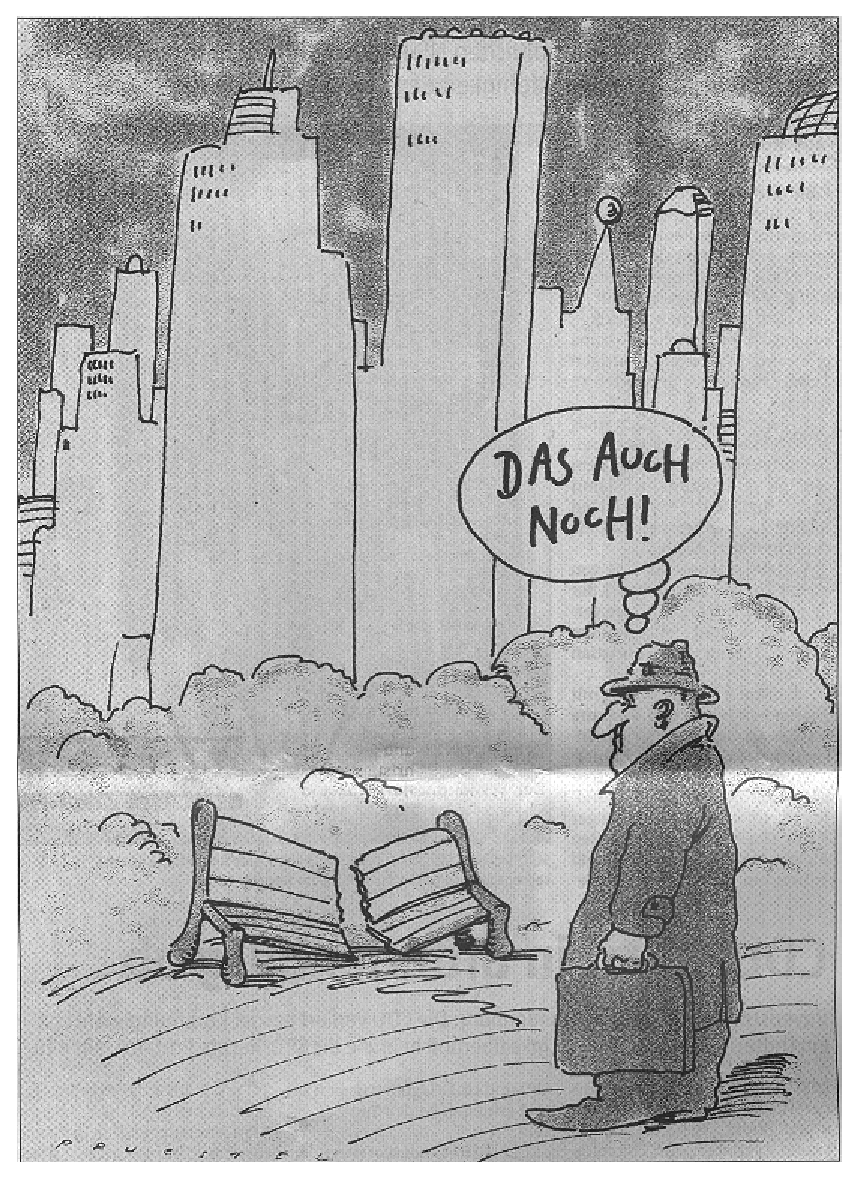
\includegraphics[width=\textwidth]{Bilder/bankenkrise}
\end{column}
\begin{column}{73mm}
Genusunterschiede nicht immer gegeben:
\eal
\ex die Bank -- die Banken
\ex die Bank -- die Bänke
\zl
\end{column}
\end{columns}
}

\frame{
\frametitle{Homonymie: grammatisch unmarkiert}


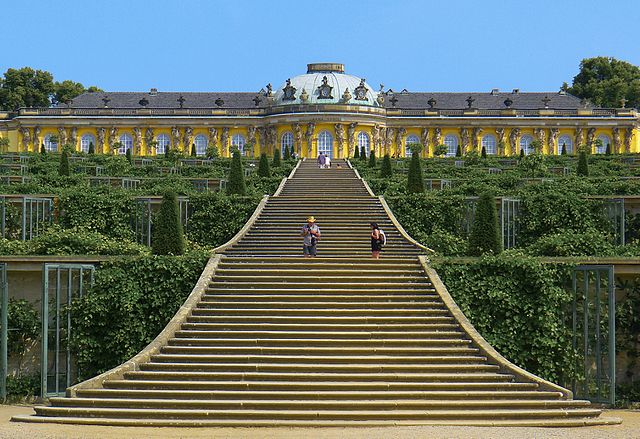
\includegraphics[width=0.6\textwidth]{material/Potsdam_sans_souci}\hfill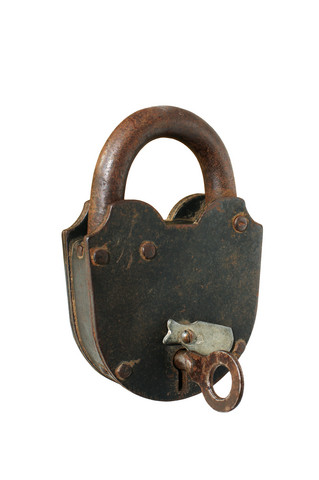
\includegraphics[width=0.3\textwidth]{material/Schloss_alt}

Wieviele Schlösser sind hier zu sehen? \\
{\scriptsize (\url{https://commons.wikimedia.org}; www.colourbox.de)}

}

%\subsubsection{Homophone und Homographen}

\begin{frame}
\frametitle{Homophone und Homographen}
  \begin{itemize}
  \item \blaubf{Homophone}
\eal
\ex Miene (Gesichtsausdruck) 
\ex Mine (Bergwerk, Sprengkörper, Stift) 
\zl
\pause
\item \blaubf{Homographen} 
\eal 
\ex übers\textprimstress etzen 
\ex \textprimstress übersetzen
\zl
\pause
\item Solche Identität von Formen ist aber relativ uninteressant,\\
      weil zufällig oder historisch begründet.
  \end{itemize}
\end{frame}


\subsubsection{Polysemie}

\begin{frame}
\frametitle{Polyseme}
  \begin{itemize}
  \item Interessanter sind Polyseme:
\eal
\ex Krone: Königskrone, Baumkrone, Schaumkrone
\ex belegen: ein Seminar/einen Platz/eine Aussage/ein Brötchen belegen
\zl
Die Lesarten unterscheiden sich, sind aber miteinander verwandt.

\pause
\item Produktive Polysemien interessant, weil sich dafür Regeln finden lassen.

% Wikipedia Metonymie
%
Beispiel: \blaubf{Metonymie} (Namensvertauschung, Umbennenung): gemeinter Gegenstand wird durch einen Ausdruck bezeichnet, der sich
auf einen anderen, aber verbundenen Gegenstand bezieht. \zb Teil für Ganzes.
\ea
Möchtest Du noch eine Tasse? = \\Möchtest Du noch eine Tasse gefüllt mit Tee?
\z
Genauso \emph{Glas}, \emph{Teller}: Gefäß für Inhalt

% Meronymie = Finger Hand
% (auch Meronymie, méros = Teil)
  \end{itemize}
\end{frame}

\begin{frame}
\frametitle{Polysemie}
  \begin{itemize}
  \item Tier für sein Fleisch.
\eal
\ex Dort drüben läuft ein Kaninchen. 
\ex Zu Ostern gab es Kaninchen.
\zl
  \end{itemize}
\end{frame}




%%%%%%%%%%%%%%%%%%%%%%%%%%%%%%%%%%%
%
\subsubsection{Sinnrelationen}
%
%\frame{
%\begin{multicols}{2}
%\frametitle{~}
%	\tableofcontents[currentsection]
%\end{multicols}
%}
%%%%%%%%%%%%%%%%%%%%%%%%%%%%%%%%%%%%%%%

\begin{frame}
\frametitle{Sinnrelationen}

\begin{itemize}
	\item Zusammenhang zwischen den Bedeutungen von Ausdrücken
	\item Systematisch erfassbare Relationen:
	
\vspace{5mm}
	
	\begin{itemize}
		\item Synonymie
		\item Hyponymie / Hyperonymie (Kohyponymie)
		\item Meronymie
 		\item Antonymie
	\end{itemize}
	
\end{itemize}

\end{frame}


%%%%%%%%%%%%%%%%%%%%%%%%%%%%%%%%%%%

\begin{frame}
\frametitle{Synonymie}

\begin{itemize}
	\item Zwei Ausdrücke X und Y sind Synonyme, wenn der Austausch von X durch Y und umgekehrt in allen Kontexten bei Wahrung der Wahrheit (salva veritate) erfolgt.
	\item[]
	\item Bikonditional: $\leftrightarrow$
	
	\eal
		\ex Apfelsine $\leftrightarrow$ Orange
		\ex anfangen $\leftrightarrow$ beginnen
		\ex sterben $\leftrightarrow$ abkratzen (in einer Bedeutung)
		\ex Treppe $\leftrightarrow$ Stiege
		\ex Brötchen $\leftrightarrow$ Schrippe $\leftrightarrow$ Semmel
	\zl
	
	\item Konnotative, regionale und registerabhängige Unterschiede
\end{itemize}

\end{frame}


%%%%%%%%%%%%%%%%%%%%%%%%%%%%%%%%%%%

\begin{frame}
\frametitle{Hyperonymie / Hyponymie}

\begin{itemize}
	\item 
Ein Ausdruck X ist ein Hyperonym von Y,\\
wenn die Bedeutung von Y in der Bedeutung von X enthalten ist.

Ein Ausdruck Y ist ein Hyponym von X,\\
wenn die Bedeutung von Y in der Bedeutung von X enthalten ist.
	\item[]	
	\item Transitive Relation
	\item[]
	\item Implikation: \ras
	
	\begin{itemize}
		\item Y ist ein X
		
		\eal 
		\ex Küchenstuhl \ras Stuhl \ras Sitzgelegenheit
		\ex erschie\ss{}en \ras töten
		\zl
		
	\end{itemize}
	
\end{itemize}

\end{frame}


%%%%%%%%%%%%%%%%%%%%%%%%%%%%%%%%%%%

\begin{frame}
\frametitle{Kohyponymie}

\begin{itemize}
\item
  Ein Ausdruck X ist ein Kohyponym von Z (und umgekehrt),\\
wenn die Bedeutung von X und Z in der Bedeutung von Y enthalten ist. 

Kohyponyme schließen einander aus (Inkompatibilität)

\eal
\ex Drehstuhl $|$ Küchenstuhl \ras Stuhl \ras Sitzgelegenheit
\ex erschießen / erwürgen / erdrosseln \ras töten
\zl


	\item[]
	\item Hyperonymie $|$ Hyponymie: Basis für Taxonomien

\end{itemize}

\end{frame}


%%%%%%%%%%%%%%%%%%%%%%%%%%%%%%%%%%

\begin{frame}
\frametitle{Meronymie}

\begin{itemize}
	\item 
Ein Ausdruck X ist ein Meronym von Y, wenn X ein Teil von Y ist.

\vspace{5mm}
	
	\eal
	\ex Finger > Hand > Arm > Oberkörper > Körper
	\ex Rad > Auto
	\zl

	\item scheint transitiv zu sein: 
		
	\ea die Manschette des Ärmels, der Ärmel der Jacke \ras die Manschette der Jacke
	\z
		
	\item Ist aber intransitiv: 
		
	\ea der Griff der Tür, die Tür des Hauses \ras \# der Griff des Hauses
	\z
		
\end{itemize}

\end{frame}


%%%%%%%%%%%%%%%%%%%%%%%%%%%%%%%%%%%

\begin{frame}
\frametitle{Antonymie}

\begin{itemize}
	\item 
Ein Ausdruck X ist ein Antonym von Y,\\
wenn X in irgendeinem Sinne das Gegenteil von Y ist.
	\item[]	
	\item X \ras $\lnot$ Y
	
	\eal 
		\ex fleißig -- faul
		\ex klug -- dumm
	\zl
	
\end{itemize}

\end{frame}


%%%%%%%%%%%%%%%%%%%%%%%%%%%%%%%%%%%

\begin{frame}
\frametitle{Kontradiktorische Antonymie}

\begin{itemize}
	\item 
Ein Ausdruck X ist ein kontradiktorisches Antonym von Y,\\
wenn die Negation von X die Bedeutung von Y ergibt und umgekehrt.\\
(Eine drittes Z ist ausgeschlossen)
	\item Komplementarität: (X \ras $\lnot$ Y) \& ($\lnot$ X  \ras Y)
	\item Binär
	\item Beide Aussagen können nicht gleichzeitig wahr sein und auch nicht gleichzeitig falsch sein.
	
	\eal
		\ex krank -- gesund
		\ex lebendig -- tot
		\ex anwesend -- abwesend
	\zl
	
\end{itemize}

\end{frame}


%%%%%%%%%%%%%%%%%%%%%%%%%%%%%%%%%%%

\begin{frame}
\frametitle{Konträre Antonymie}

\begin{itemize}
	\item
Ein Ausdruck X ist ein konträres Antonym von Y,\\
wenn X und Y nicht zugleich wahr sein können,\\
aber beide können zugleich nicht zutreffen.
	\item[]
	\item Skalar: Antonymie mit Zwischenstufen
	\item[]
	\item Beide Aussagen können nicht gleichzeitig wahr sein,\\
              aber sie können gleichzeitig falsch sein.
	\item[]
	\item (X $\rightarrow \lnot$ Y) \& (Y $\rightarrow \lnot$ X)
	
	\eal
		\ex reich -- arm
		\ex kalt -- (kühl -- lau -- warm) -- heiß
	\zl
	
\end{itemize}

\end{frame}


%% %%%%%%%%%%%%%%%%%%%%%%%%%%%%%%%%%%%

%% \begin{frame}
%% \frametitle{Sinnrelationen}

%% \begin{itemize}
%% 	\item \textbf{Ambiguität (Lexikalische Mehrdeutigkeit)}

%% \vspace{1em}

%% 	\begin{itemize}
%% 		\item \textbf{Homonymie}\\
%% Ein Ausdruck X und ein Ausdruck Y sind gleich in deren Form (phonetische oder graphische) aber unterschiedlich in deren Bedeutung, wobei X und Y unterschiedliche Ursprünge haben.
%% 	\end{itemize}
%% \end{itemize}

%% \end{frame}


%% %%%%%%%%%%%%%%%%%%%%%%%%%%%%%%%%%%%

%% \begin{frame}
%% \frametitle{Sinnrelationen}

%% \begin{itemize}
%% 	\item \textbf{Ambiguität (Lexikalische Mehrdeutigkeit)}

%% \vspace{1em}

%% 	\begin{itemize}
%% 		\item \textbf{Homonymie:}
		
%% 		\begin{itemize}
%% 			\item Homophonie:
			
%% 			\eal
%% 			\ex mahlen vs. malen 
%% 			\ex sieben (7) vs. sieben
%% 			\ex laut vs. laut (Präp.)
%% 			\zl
			
%% 			\item Homographie:
					
%% 			\eal 
%% 			\ex 'modern vs. mo'dern
%% 			\ex Die Therapie des gebrochenen Beines beinhaltet das Fixieren in einer Beinhalterung.
%% 			\zl
			
%% 		\end{itemize}
		
%% 	\end{itemize}
%% \end{itemize}

%% \end{frame}


%% %%%%%%%%%%%%%%%%%%%%%%%%%%%%%%%%%%%

%% \begin{frame}
%% \frametitle{Sinnrelationen}

%% \begin{itemize}
%% 	\item \textbf{Ambiguität (Lexikalische Mehrdeutigkeit)}
	
%% \vspace{1em}

%% 	\begin{itemize}
%% 		\item \textbf{Polysemie}\\
%% Ein Ausdruck X und ein Ausdruck Y sind gleich in deren Form (phonetische und graphische) können aber unterschiedliche Bedeutungsvarianten voneinander sein. X und Y stehen in einem etymologischen Zusammenhang zueinander.

%% 		\ea Schule, Oper, Grammatik
%% 		\z

%% 	\end{itemize}
	
%% \end{itemize}

%% \end{frame}


%%%%%%%%%%%%%%%%%%%%%%%%%%%%%%%%%%%
\iftoggle{uebung}{

\begin{frame}
\frametitle{Sinnrelationen}

\begin{itemize}
	\item \textbf{Übung:}
	
	\eal
	\ex Ballkleid -- Kleid
	\ex Bank -- Bank
	\ex Schraubenzieher -- Zange
	\ex gro\ss{} -- klein
	\ex Henkel -- Tasse
	\ex Ahorn -- Baum
	\ex essen -- verzehren
	\ex gerade -- ungerade
	\zl
		
\end{itemize}

\end{frame}


%%%%%%%%%%%%%%%%%%%%%%%%%%%%%%%%%%%%%%%%%
%\iftoggle{loesung}{

\begin{frame}
\frametitle{Sinnrelationen: Lösung}
	
	\eal
	\ex Ballkleid -- Kleid: Hyponym/Hyperonym
	\ex Bank -- Bank: Homonymie (-graphie und -phonie)
	\ex Schraubenzieher -- Zange: Kohyponymie
	\ex gro\ss{} -- klein: Konträre Antonymie
	\ex Henkel -- Tasse: Meronymie
	\ex Ahorn -- Baum: Hyponym/Hyperonym
	\ex essen -- verzehren: Synonymie
	\ex gerade -- ungerade: Kontradiktorische Antonymie
	\zl

\end{frame}
%}

}

%%%%%%%%%%%%%%%%%%%%%%%%%%%%%%%%%%%%%%%%%%%
%
\subsection{Satzsemantik (Satzbedeutung)}
%
\iftoggle{toc}{
\frame{
\begin{multicols}{2}
\frametitle{~}
	\tableofcontents[currentsection]
\end{multicols}
}
}
%%%%%%%%%%%%%%%%%%%%%%%%%%%%%%%%%%%%%%%%%%

\outline{

\begin{itemize}
\item Ebenen linguistischer Analyse
\item Wörtliche Bedeutung: Abgrenzunug zur Pragmatik
\item Lexikalische Semantik
\item \blaubf{Satzsemantik}
\end{itemize}

}



\begin{frame}
\frametitle{Satzsemantik (Satzbedeutung)}

\begin{itemize}
	\item Wahrheitsbedingungen (\citeauthor{Wittgenstein72a-u} 1921)
	\item[]
	\item Die Bedeutung eines Satzes zu kennen, heißt, notwendige und hinreichende Bedingungen für die Wahrheit bzw. Falschheit des Satzes (= seine Wahrheitsbedingungen) zu kennen.
	\item[]
	\item Bedingungen in der aktuellen Welt (verschiedene Welten)
	
	
		\ea Martin kauft Brötchen.
		\z
		
	\begin{itemize}	
		\item Wahr oder Falsch (1 oder 0) \ras abhängig von der Welt
	\end{itemize}
	
\end{itemize}

\end{frame}


%%%%%%%%%%%%%%%%%%%%%%%%%%%%%%%%%%%%%%%%%%

\begin{frame}
\frametitle{Satzsemantik (Satzbedeutung)}

\begin{itemize}
	\item \textbf{Kompositionalitätsprinzip}\\
Die Bedeutung eines komplexen Ausdrucks ergibt sich aus der Bedeutung seiner unmittelbaren syntaktischen Teile und der Art und Weise, wie sie sich syntaktisch zusammensetzen.
	\item[]
	\item Auch Fregeprinzip genannt
\end{itemize}

\end{frame}


%%%%%%%%%%%%%%%%%%%%%%%%%%%%%%%%%%%%%%%%%%
%%%%%%%%%%%%%%%%%%%%%%%%%%%%%%%%%%%%%%%%%%
%
\subsubsection{Aussagenlogik}
%\frame{
%\begin{multicols}{2}
%\frametitle{~}
%	\tableofcontents[currentsection]
%\end{multicols}
%}
%%%%%%%%%%%%%%%%%%%%%%%%%%%%%%%%%%%%%%%%%%


\begin{frame}
\frametitle{Aussagenlogik}

\begin{itemize}
	\item Basierend auf dem Kompositionalitätsprinzip
	\item Teilgebiet der formalen Logik
	\item Verknüpfung von einfachen Aussagen
	\item Wie lässt sich der Wahrheitswert einer komplexen Aussage aus den Wahrheitswerten der in ihr enthaltenen einfachen Aussagen in Abhängigkeit der Verknüpfung errechnen?
\end{itemize}

\end{frame}


%%%%%%%%%%%%%%%%%%%%%%%%%%%%%%%%%%%%%%%%%%

\subsubsubsection{Konnektoren}

\begin{frame}
\frametitle{Konnektoren}

\begin{itemize}
	\item Aussagen: p, q, r, s, \dots
	\item Konnektoren:
	
	\begin{itemize}
		\item Negation (NICHT): $\lnot$
		
		\item Konjunktion (UND): $\land$
		
		\item Disjunktion (UND/ODER): $\lor$
		
		\item Konditional (materiale Implikation) (WENN, DANN): \ras
		
		\item Bikonditional (GENAU DANN WENN): $\leftrightarrow$
	\end{itemize}
	
\end{itemize}

\end{frame}


%%%%%%%%%%%%%%%%%%%%%%%%%%%%%%%%%%%%%%%%%%

\begin{frame}
\frametitle{Negation}

\begin{itemize}
	\item Negation (NICHT): $\lnot$
	
	\eal
		\ex p: Es regnet.
		\ex $\lnot$ p: Es regnet nicht.
	\zl
	
\end{itemize}

\begin{table}
\centering
\begin{tabular}{p{3cm}|p{3cm}}
\textbf{p} & \textbf{$\lnot$p}\\
\hline
1 & 0\\
\hline
0 & 1\\
\end{tabular}
\end{table}

\end{frame}


%%%%%%%%%%%%%%%%%%%%%%%%%%%%%%%%%%%%%%%%%%

\begin{frame}
\frametitle{Konjunktion}

\begin{itemize}
	\item Konjunktion (UND): $\land$
	
	\eal
		\ex p: Es regnet.
		\ex q: Es donnert.
		\ex p $\land$ q: Es regnet und es donnert.
	\zl

\end{itemize}
	

\begin{table}
\centering

\begin{tabular}{p{2cm}|p{2cm}|p{2cm}}
\textbf{p} & \textbf{q} & \textbf{p} $\land$ \textbf{q}\\
\hline
1 & 1 & 1\\
\hline
1 & 0 & 0\\
\hline
0 & 1 & 0\\
\hline 
0 & 0 & 0\\
\end{tabular}

\end{table}	

\end{frame}


%%%%%%%%%%%%%%%%%%%%%%%%%%%%%%%%%%%%%%%%%%

\begin{frame}
\frametitle{Disjunktion}

\begin{itemize}
	\item Disjunktion (UND/ODER): $\lor$

	\eal
		\ex p: Es regnet.
		\ex q: Es schneit.
		\ex p $\lor$ q : Es regnet oder es schneit.
	\zl

\end{itemize}


\begin{table}
\centering

\begin{tabular}{p{2cm}|p{2cm}|p{2cm}}
\textbf{p} & \textbf{q} & \textbf{p} $\lor$ \textbf{q}\\
\hline
1 & 1 & 1\\
\hline
1 & 0 & 1\\
\hline
0 & 1 & 1\\
\hline 
0 & 0 & 0\\
\end{tabular}

\end{table}		

\end{frame}


%%%%%%%%%%%%%%%%%%%%%%%%%%%%%%%%%%%

\begin{frame}
\frametitle{Konditional (Implikation)}

\begin{itemize}
	\item Konditional (materiale Implikation) (WENN, DANN): \ras
	
	\eal
		\ex p: Es regnet.
		\ex q: Die Stra\ss{}e ist nass.
		\ex p \ras q : Wenn es regnet, dann ist die Stra\ss{}e nass.
	\zl

\end{itemize}

\begin{table}
\centering
\begin{tabular}{p{2cm}|p{2cm}|p{2cm}}
\textbf{p} & \textbf{q} & \textbf{p} \ras \textbf{q}\\
\hline
1 & 1 & 1\\
\hline
1 & 0 & 0\\
\hline
0 & 1 & 1 (!)\\
\hline 
0 & 0 & 1\\
\end{tabular}
\end{table}	


\end{frame}


%%%%%%%%%%%%%%%%%%%%%%%%%%%%%%%%%%%

\begin{frame}
\frametitle{Bikonditional}

\begin{itemize}
	\item Bikonditional (GENAU DANN WENN): $\leftrightarrow$
	
	\eal
		\ex p: Peter raucht.
		\ex q: Maria trinkt.
		\ex p $\leftrightarrow$ q : Genau dann wenn Peter raucht, trinkt Maria.
	\zl

\end{itemize}


\begin{table}
\centering

\begin{tabular}{p{2cm}|p{2cm}|p{2cm}}
\textbf{p} & \textbf{q} & \textbf{p} $\leftrightarrow$ \textbf{q}\\
\hline
1 & 1 & 1\\
\hline
1 & 0 & 0\\
\hline
0 & 1 & 0\\
\hline 
0 & 0 & 1\\
\end{tabular}

\end{table}

\end{frame}


%%%%%%%%%%%%%%%%%%%%%%%%%%%%%%%%%%%
\iftoggle{uebung}{

\begin{frame}
\frametitle{Übung}

\begin{itemize}
	\item Stellen Sie folgende Sätze als Verknüpfung von Satzvariablen dar.\\Geben Sie die
          Wahrheitswertetabellen an.
	
	\vspace{1em}
	
	\begin{enumerate}
		\item Christiane schläft.

		\item Norbert raucht nicht.
		
		\item Norbert raucht und Christiane schläft nicht.
		
		\item Wenn Norbert nicht raucht, schläft Christiane nicht.
		
		\item Wenn ich schlafe, träume ich.
		
		\item Ich schlafe nicht oder ich träume.
	\end{enumerate}
	
\end{itemize}

\end{frame}

%%%%%%%%%%%%%%%%%%%%%%%%%%%%%%%%%%%

%%%%%%%%%%%%%%%%%%%%%%%%%%%%%%%%%%%
%\iftoggle{loesung}{

\begin{frame}
\frametitle{Lösungen}

\begin{table}

\begin{minipage}{0.3\textwidth}
\centering
\begin{itemize}
\item[] \small{p: Christiane schläft.}
\end{itemize}
\scalebox{0.8}{
\begin{tabular}{l}
p\\
\hline
1\\
\hline
0\\
\end{tabular}
}
\end{minipage}
%	
\begin{minipage}{0.65\textwidth}
\centering
\begin{itemize}
\item[] \small{Norbert raucht und Christiane schläft nicht.\\
               p: Norbert raucht.\\
               q: Christiane schläft.}
\end{itemize}
\scalebox{0.8}{
\begin{tabular}{l|l|l|c}
p & q & $\lnot$ q & p $\land \lnot $q\\
\hline
1 & 1 & 0 & 0\\
\hline
1 & 0 & 1 & 1\\
\hline
0 & 1 & 0 & 0 \\
\hline
0 & 0 & 1 & 0 \\
\end{tabular}
}
\end{minipage}

\vspace{1em}

\begin{minipage}{0.3\textwidth}
\centering
\begin{itemize}
\item[] \small{Norbert raucht nicht.\\
               p: Norbert raucht.}
\end{itemize}
\scalebox{0.8}{
\begin{tabular}[b]{l|l}
p & $ \lnot $p \\
\hline
0 & 1 \\
\hline
1 & 0 \\
\end{tabular}}
\end{minipage}
%
\begin{minipage}{0.65\textwidth}
\centering
\begin{itemize}
\item[] \small{Wenn Norbert nicht raucht, schläft Christiane nicht.\\
               p: Norbert raucht.\\
               q: Christiane schläft.}
\end{itemize}
\scalebox{0.8}{
\begin{tabular}{l|l|c|c|c}
p & q & $ \lnot $p& $ \lnot $q &$ \lnot $p \ras $ \lnot $q\\
\hline
1 & 1 & 0 & 0 & 1 \\
\hline
1 & 0 & 0 & 1 & 1\\
\hline
0 & 1 & 1 & 0 & 0 \\
\hline
0 & 0 & 1 & 1 & 1 \\
\end{tabular}}
\end{minipage}
\end{table}

\end{frame}

%
%%%%%%%%%%%%%%%%%%%%%%%%%%%%%%%%%%%%

\begin{frame}
\frametitle{Lösungen}

\begin{table}

\begin{minipage}{0.48\textwidth}
\centering
\begin{itemize}
\item[] \small{Wenn ich schlafe, träume ich.\\
               p: Ich schlafe.\\
               q: Ich träume.}
\end{itemize}
\scalebox{0.8}{
\begin{tabular}[b]{l|l|c}
p & q & p \ras q \\
\hline
1 & 1 & 1 \\
\hline
1 & 0 & 0 \\
\hline
0 & 1 & 1 \\
\hline
0 & 0 & 1 \\
\end{tabular}}
\end{minipage}
%
\begin{minipage}{0.48\textwidth}
\centering
\begin{itemize}
\item[] \small{Ich schlafe nicht oder ich träume.\\
               p: Ich schlafe.\\
               q: Ich träume.}
\end{itemize}
\scalebox{0.8}{
\begin{tabular}{l|l|l|c}
p & q & $\lnot$p & $\lnot $p $\lor$ q\\
\hline
1 & 1 & 0  & 1 \\
\hline
1 & 0 & 0  & 0 \\
\hline
0 & 1 & 1 & 1 \\
\hline
0 & 0 & 1 & 1 \\
\end{tabular}}
\end{minipage}
\end{table}

\end{frame}
%}
%
}


%%%%%%%%%%%%%%%%%%%%%%%%%%%%%%%%%%%%

\iftoggle{uebung}{
\begin{frame}
\frametitle{Übung}

\begin{itemize}
	\item Stellen Sie folgende Sätze als Verknüpfung von Satzvariablen dar.\\ Geben Sie die
          Wahrheitswertetabellen an.

\vspace{1em}

	\begin{enumerate}
		\item Genau dann wenn ich Durst habe, trinke ich eine Cola.
		
		\item Es ist nicht der Fall, dass ich Durst habe, und es ist nicht der Fall, dass ich eine Cola trinke -- oder -- Es ist der Fall, dass ich Durst habe und es ist der Fall, dass ich eine Cola trinke.
		
		\item Es regnet oder, es scheint die Sonne und ich bin froh.
		
		\item Es regnet oder es scheint die Sonne, und es regnet oder ich bin froh.
		
		\item Es ist nicht der Fall, dass Norbert raucht oder Christiane schläft.
		
		\item Es ist nicht der Fall, dass Norbert raucht, und es ist nicht der Fall, dass Christiane schläft.
	\end{enumerate}
		
\end{itemize}


\end{frame}

%%%%%%%%%%%%%%%%%%%%%%%%%%%%%%%%%%%%%%%%%%%%%%%%%%%%%%%%%%%%%%%

%\iftoggle{loesung}{

\begin{frame}
\frametitle{Lösungen}


\begin{itemize}
\item[] Genau dann wenn ich Durst habe, trinke ich eine Cola.\\
		p: Ich habe Durst.\\
                q: Ich trinke eine Cola.

\medskip

\begin{tabular}{l|l|c}
p & q & p $ \leftrightarrow $ q\\
\hline
1 & 1 & 1\\
\hline
1 & 0 & 0\\
\hline
0 & 1 & 0\\
\hline
0 & 0 & 1\\
\end{tabular}
\end{itemize}


\end{frame}

\begin{frame}
\frametitle{Lösungen}


%	
\begin{itemize}
\item[] 
Es ist nicht der Fall, dass ich Durst habe, und\\
es ist nicht der Fall, dass ich eine Cola trinke -- oder -- \\
Es ist der Fall, dass ich Durst habe und\\
es ist der Fall, dass ich eine Cola trinke.\\

\medskip

p: Ich trinke Cola.\\
q: Ich habe Durst.

\bigskip

\begin{tabular}{l|l|c|c|c|c|c}
p & q & $\lnot$ p & $\lnot$ q & $ \lnot $p $ \land$ $\lnot $q & p $ \land $ q & ($ \lnot $p $ \land \lnot $q) $ \lor $ (p $ \land $ q)\\
\hline
1 & 1 & 0& 0 & 0 & 1 & 1\\
\hline
1 & 0 & 0 & 1 &  0 & 0 & 0\\
\hline
0 & 1 & 1 & 0 & 0 & 0 & 0\\
\hline
0 & 0 & 1 & 1 & 1 & 0 & 1\\
\end{tabular}

\bigskip

\item[] Das ist genau wie das GENAU DANN, WENN auf der vorigen Folie.

\end{itemize}

\end{frame}

\begin{frame}
\frametitle{Lösungen}

\begin{itemize}
\item[] Es regnet oder, es scheint die Sonne und ich bin froh.\\		
p: Es regnet.\\
q: Es scheint die Sonne.\\
s: Ich bin froh.

\bigskip

\begin{tabular}{l|l|l|c|c}
p & q & s & q $\land $ s & p $\lor$ (q $\land $ s) \\
\hline
1 & 1 & 1 & 1 & 1\\
\hline
1 & 1 & 0 & 0 & 1\\
\hline
1 & 0 & 1 & 0 & 1\\
\hline
1 & 0 & 0 & 0 & 1\\
\hline
0 & 1 & 1 & 1 & 1\\
\hline
0 & 1 & 0 & 0 & 0\\
\hline
0 & 0 & 1 & 0 & 0\\
\hline
0 & 0 & 0 & 0 & 0\\
\end{tabular}

\end{itemize}

\end{frame}

\begin{frame}
\frametitle{Lösungen}


\begin{itemize}
\item[] Es regnet oder es scheint die Sonne, und es regnet oder ich bin froh.\\
p: Es regnet.\\
q: Es scheint die Sonne.\\
s: Ich bin froh.
\end{itemize}
\begin{tabular}[b]{l|l|l|c|c|c}
p & q & s & p $ \lor $ q & p $ \lor $ s & (p $ \lor $ q) $ \land $ (p $ \lor $ s) \\
\hline
1 & 1 & 1 & 1 & 1 & 1\\
\hline
1 & 1 & 0 & 1 & 1 & 1\\
\hline
1 & 0 & 1 & 1 & 1 & 1\\
\hline
1 & 0 & 0 & 1 & 1 & 1\\
\hline
0 & 1 & 1 & 1 & 1 & 1\\
\hline
0 & 1 & 0 & 1 & 0 & 0\\
\hline
0 & 0 & 1 & 0 & 1 & 0\\
\hline
0 & 0 & 0 & 0 & 0 & 0\\

\end{tabular}

\bigskip

(p $ \lor $ q) $ \land $ (p $ \lor $ s) ist äquivalent zu p $\lor$ (q $\land $ s) (auf der vorigen Folie).

\end{frame}

%%%%%%%%%%%%%%%%%%%%%%%%%
\begin{frame}
\frametitle{Lösungen}


\begin{itemize}
\item[] Es ist nicht der Fall, dass Norbert raucht oder Christiane schläft.\\
p: Norbert raucht.\\
q: Christiane schläft.

\bigskip

\begin{tabular}{l|l|c}
p & q & $ \lnot $ (p $ \lor$ q)\\
\hline
1 & 1 & 0 \\
\hline
1 & 0 & 0 \\
\hline
0 & 1 & 0 \\
\hline
0 & 0 & 1 \\
\end{tabular}
\end{itemize}


\end{frame}

\begin{frame}
\frametitle{Lösungen}


\begin{itemize}
\item[] Es ist nicht der Fall, dass Norbert raucht, und\\
        es ist nicht der Fall, dass Christiane schläft.\\
p: Norbert schläft.\\
q: Christine schläft.

\bigskip

\begin{tabular}{l|l|c|c|c}
p & q & $\lnot$ p & $\lnot$ q & $ \lnot $p $ \land $ $ \lnot $q\\
\hline
1 & 1 & 0 & 0 & 0\\
\hline
1 & 0 & 0 & 1 & 0\\
\hline
0 & 1 & 1 & 0 & 0\\
\hline
0 & 0 & 1 & 1 & 1\\
\end{tabular}

\bigskip

\item[] $\lnot $p $ \land $ $ \lnot $q ist äquivalent zu $\lnot $ (p $ \lor$ q) (auf der vorigen Folie)

\end{itemize}

\end{frame}
%}
}% if uebung

%%%%%%%%%%%%%%%%%%%%%%%%%%%%%%%%%%%

\iftoggle{uebung}{
\begin{frame}
\frametitle{Übung Konditional}
	
\begin{itemize}
	\item Berechnen Sie die Wahrheitswertetabellen der jeweiligen Ausdrücke und zeigen Sie deren Äquivalenz:

\vspace{1em}

	\begin{enumerate}
%		\item Christiane schläft. (p)
		
%		\item Norbert raucht nicht. ($\lnot$p)
		
		\item Norbert raucht und Christiane schläft nicht. (p $\land$ $\lnot$ q)
		
		\item Wenn Norbert nicht raucht, schläft Christiane nicht. ($\lnot$ p \ras $\lnot$ q)
	\end{enumerate}

\item Konditional:

	\begin{enumerate}\setcounter{enumi}{2}
		\item Wenn ich schlafe, träume ich. ( p \ras q)
		
		\item Ich schlafe nicht oder ich träume. ($\lnot$ p $\lor$ q)
	\end{enumerate}
	
\end{itemize}

\end{frame}


%%%%%%%%%%%%%%%%%%%%%%%%%%%%%%%%%%%

\begin{frame}
\frametitle{Übung Bikonditional/Distributitvität}

\begin{itemize}
	\item Berechnen Sie die Wahrheitswertetabellen der jeweiligen Ausdrücke und zeigen Sie deren Äquivalenz:
	
\vspace{1em}

	\begin{itemize}
		\item Bikonditional:
	
		\begin{enumerate}
			\item Genau dann wenn ich Durst habe, trinke ich eine Cola. (p $\leftrightarrow$ q)
			
			\item Es ist nicht der Fall, dass ich Durst habe, und es ist nicht der Fall, dass ich eine Cola trinke – oder – Es ist der Fall, dass ich Durst habe, und es ist der Fall, dass ich eine Cola trinke. ($\lnot$ p $\wedge$ $\lnot$ q) $\lor$ (p $\wedge$ q)
		\end{enumerate}
	
		\item Distributivität:
	
		\begin{enumerate}\setcounter{enumi}{2}
			\item Es regnet oder -- es scheint die Sonne und ich bin froh. (p  $\lor$ (q $\land$ r))
			
			\item Es regnet oder es scheint die Sonne, und es regnet oder ich bin froh. ((p $\lor$ q) $\land$ (p $\lor$ r))
		\end{enumerate}

	\end{itemize}

\end{itemize}



\end{frame}


%%%%%%%%%%%%%%%%%%%%%%%%%%%%%%%%%%%

\begin{frame}
\frametitle{Übung De Morgans Gesetze}

\begin{itemize}
\item Berechnen Sie die Wahrheitswertetabellen der jeweiligen Ausdrücke und zeigen Sie deren Äquivalenz:

	\begin{itemize}
		\item De Morgans Gesetze ($\lnot$ (p $\lor$ q) $\equiv$ $\lnot$ p $\land$ $\lnot$ q):
	
		\begin{enumerate}
			\item Es ist nicht der Fall, dass Norbert raucht oder Christiane schläft. $\lnot$ (p $\lor$ q)
			
			\item Es ist nicht der Fall, dass Norbert raucht, und es ist nicht der Fall, dass Christiane schläft. ($\lnot$ p $\land \lnot$ q)
		\end{enumerate}
		
	\end{itemize}

\end{itemize}


\end{frame}
}


%%%%%%%%%%%%%%%%%%%%%%%%%%%%%%%%%%%

\begin{frame}
\frametitle{Tautologie, Kontradiktion, Kontingenz}

\begin{itemize}
	\item \textbf{Tautologie}
	
	\begin{itemize}
	\item Aussage, die stets wahr ist\\
          (unabhängig von den Ausgangswerten der beteiligten Aussagen)
		
		\ea Es regnet oder es regnet nicht.
		\z
		
	\end{itemize}
	
	\item \textbf{Kontradiktion}
	
	\begin{itemize}
	\item  Aussage, die stets falsch ist\\
          (unabhängig von den Ausgangswerten der beteiligten Aussagen)

		\ea Es regnet und es regnet nicht.
		\z
		
	\end{itemize}
	
	\item \textbf{Kontigenz}
	
	\begin{itemize}
		\item Aussage, die abhängig von den Ausgangswerten der beteiligten Aussage sowohl wahr als auch falsch sein kann.

		\ea Es regnet oder es schneit.
		\z

	\end{itemize}
	
\end{itemize}


\end{frame}


%%%%%%%%%%%%%%%%%%%%%%%%%%%%%%%%%%%

\begin{frame}
\frametitle{Übung}

\begin{itemize}
	\item Überprüfen Sie die Richtigkeit der folgenden Beispiele:
	
	\vspace{1em}
	
	\begin{itemize}
		\item Tautologien:
	
		\eal
			\ex (p $\lor$ $\lnot$p)
			\ex (p $\rightarrow$ p)
			\ex $\lnot$ (p $\land$ $\lnot$p)
		\zl
			
		\item Kontradiktionen:
		
		\eal
			\ex $\lnot$ (p $\lor$ $\lnot$p)
			\ex $\lnot$ ((p $\lor$ q) $\leftrightarrow$ (q $\lor$ p))
		\zl

		\item Kontingenzen:
		
		\eal
			\ex ((p $\lor$ q) $\rightarrow$ q)
			\ex ((p $\rightarrow$ q) $\leftrightarrow$ (q $\rightarrow$ p))
		\zl
			
	\end{itemize}	
	
\end{itemize}

\end{frame}


\author{Stefan Müller}

\subsubsection{Bedeutung von Ausdrücken}

\begin{frame}
\frametitle{Bedeutung von Ausdrücken: \emph{Kind}}

Ein Nomen bezieht sich auf eine Menge von Objekten,\\
        die die entsprechenden Eigenschaft haben:\\
        \emph{Kind} steht für alle Kinder in einer bestimmten Situation.

%\centerline{%
\begin{pspicture}[unit=8mm](-1,0)(11,4.5)
%\psgrid
\rnode{D}{\psframe(0,0)(8,5)}
\pscircle[fillcolor=beamer@fugreen,fillstyle=solid](1,1){0.1}
\pscircle[fillcolor=beamer@fugreen,fillstyle=solid](2,2){0.1}
\pscircle[fillcolor=beamer@fugreen,fillstyle=solid](4,2){0.1}
\pscircle[fillcolor=beamer@fugreen,fillstyle=solid](3,3){0.1}
\pscircle[fillcolor=beamer@fugreen,fillstyle=solid](7,4){0.1}
\rput[Bl](5,3){%
\rnode{Kind}{Kind}}
%
\cnode(3,2){1.5}{KindSet}
\ncline[nodesepA=0pt,nodesepB=2pt]{KindSet}{Kind}
%
\rput[Bl](9,2){%
\rnode{Diskursuniversum}{\begin{tabular}{@{}l@{}}
                         Diskurs-\\
                         universum (Welt)\\
                         \end{tabular}}}
%\ncline[nodesepA=0pt,nodesepB=2pt]{D}{Diskursuniversum}
\psline(8.9,2.4)(8,2.4)
%
%
%\psellipse(4,2)(3,1.5)
%\anodeconnect[l]{modell}[r]{phen}%
\end{pspicture}
%}


\end{frame}


\begin{frame}
\frametitle{Bedeutung von Ausdrücken: Eigennamen}

Eigennamen bezeichnen Individuen.\\
Ein Individuum kann mehrere Namen haben oder keinen.

%\centerline{%
%{
\begin{pspicture}[unit=8mm](-1,0)(11,4.5)
%\psgrid
\psframe(0,0)(8,5)
\rput[Bl](2.6,1.2){%
\rnode{Max}{Max}}
\rput[Bl](1,3){%
\rnode{Dicker}{Dicker}}
\rput[Bl](4,3){%
\rnode{Chantalle}{Chantalle}}
\rput[Bl](2,.5){%
\rnode{Barbara}{Barbara}}

\cnode[fillcolor=beamer@fugreen,fillstyle=solid](1,1){0.1}{BarbaraDot}
\cnode[fillcolor=beamer@fugreen,fillstyle=solid](2,2){0.1}{MaxDot}
\cnode[fillcolor=beamer@fugreen,fillstyle=solid](4,2){0.1}{NonameDot}
\cnode[fillcolor=beamer@fugreen,fillstyle=solid](3,3){0.1}{ChantalleDot}
\cnode[fillcolor=beamer@fugreen,fillstyle=solid](7,4){0.1}{NoName2Dot}
%
%\psellipse(4,2)(3,1.5)
%\anodeconnect[l]{modell}[r]{phen}%
\ncline[nodesepA=2pt,nodesepB=0pt]{Barbara}{BarbaraDot}
\ncline[nodesepA=2pt,nodesepB=0pt]{Max}{MaxDot}
\ncline[nodesepA=2pt,nodesepB=0pt]{Dicker}{MaxDot}
\ncline[nodesepA=2pt,nodesepB=0pt]{Chantalle}{ChantalleDot}
\end{pspicture}
%}


\end{frame}


\begin{frame}
\frametitle{Bedeutung von Ausdrücken: \emph{klug}}

        \emph{klug} steht für alle klugen Individuen in einer bestimmten Situation.

%\centerline{%
%{
\begin{pspicture}[unit=8mm](-1,0)(11,4.5)
%\psgrid
\psframe(0,0)(8,5)
\pscircle[fillcolor=beamer@fugreen,fillstyle=solid](1,1){0.1}
\pscircle[fillcolor=beamer@fugreen,fillstyle=solid](2,2){0.1}
\pscircle[fillcolor=beamer@fugreen,fillstyle=solid](4,2){0.1}
\pscircle[fillcolor=beamer@fugreen,fillstyle=solid](3,3){0.1}
\pscircle[fillcolor=beamer@fugreen,fillstyle=solid](7,4){0.1}
\rput[Bl](3,0.5){%
\rnode{klug}{klug}}
%
\cnode(1.5,1.5){1}{klugSet}
\ncline[nodesepA=0pt,nodesepB=2pt]{klugSet}{klug}
\end{pspicture}
%}


\end{frame}



\begin{frame}
\frametitle{Bedeutung von Ausdrücken: \emph{kluges Kind}}

Ein \emph{kluges Kind} ist sowohl klug als auch Kind.

%\centerline{%
%{
\begin{pspicture}[unit=8mm](-1,0)(11,4.5)
%\psgrid
\psframe(0,0)(8,5)
\rput[Bl](5,3){%
\rnode{Kind}{Kind}}
%
\cnode(3,2){1.5}{KindSet}
\ncline[nodesepA=0pt,nodesepB=2pt]{KindSet}{Kind}
\rput[Bl](0.5,3.5){%
\rnode{klug}{klug}}
%
\cnode(1.5,1.5){1}{klugSet}
\ncline[nodesepA=0pt,nodesepB=2pt]{klugSet}{klug}
\psclip
{%
\pscircle(3,2){1.5}
}
\pscircle[fillstyle=hlines](1.5,1.5){1}
\endpsclip
\pscircle[fillcolor=beamer@fugreen,fillstyle=solid](1,1){0.1}
\pscircle[fillcolor=beamer@fugreen,fillstyle=solid](2,2){0.1}
\pscircle[fillcolor=beamer@fugreen,fillstyle=solid](4,2){0.1}
\pscircle[fillcolor=beamer@fugreen,fillstyle=solid](3,3){0.1}
\pscircle[fillcolor=beamer@fugreen,fillstyle=solid](7,4){0.1}
%
%\psellipse(4,2)(3,1.5)
%\anodeconnect[l]{modell}[r]{phen}%
\end{pspicture}
%}


\end{frame}


\begin{frame}
\frametitle{Bedeutung von Ausdrücken: \emph{Alle klugen Kinder schlafen}}

\emph{Alle klugen Kinder schlafen} ist in folgender Welt wahr:

%\centerline{%
%{
\begin{pspicture}[unit=8mm](-1,0)(11,4.5)
%\psgrid
\psframe(0,0)(8,5)
\rput[Bl](5,3){%
\rnode{Kind}{Kind}}
%
\cnode(3,2){1.5}{KindSet}
\ncline[nodesepA=0pt,nodesepB=2pt]{KindSet}{Kind}
\rput[Bl](0.5,3.5){%
\rnode{klug}{klug}}
%
\cnode(1.5,1.5){1}{klugSet}
\ncline[nodesepA=0pt,nodesepB=2pt]{klugSet}{klug}
\psclip
{%
\pscircle(3,2){1.5}
}
\pscircle[fillstyle=hlines](1.5,1.5){1}
\endpsclip
\pscircle[fillcolor=beamer@fugreen,fillstyle=solid](1,1){0.1}
\pscircle[fillcolor=beamer@fugreen,fillstyle=solid](2,2){0.1}
\pscircle[fillcolor=beamer@fugreen,fillstyle=solid](4,2){0.1}
\pscircle[fillcolor=beamer@fugreen,fillstyle=solid](3,3){0.1}
\pscircle[fillcolor=beamer@fugreen,fillstyle=solid](7,4){0.1}
%
\rput*[refpoint]{45}(2.5,-1){\psellipse(2.5,2.5)(1.8,0.9)}
\rput[Bl](4.5,4){%
\rnode{schlafen}{schlafen}}
\psline(4.3,4.1)(3.8,3.8)
\ncline[nodesepA=0pt,nodesepB=2pt]{schlafenSet}{schlafen}
%\anodeconnect[l]{modell}[r]{phen}%
\end{pspicture}
%}

Für alle, für die gilt, dass sie klug und Kinder sind, gilt auch,\\
dass sie schlafen. 

\end{frame}

\begin{frame}[shrink=15]
\frametitle{Bedeutung von Determinatoren}

Determinatoren: \zb Quantoren (ein, alle), definite Artikel 
\eal
\ex Alle Kinder schlafen.
\ex Für alle x, für die gilt, dass sie Kind sind, gilt auch, dass sie schlafen.
\ex \blau{$\forall$}x kind(x) \blau{$\to$} schlafen(x)
\zl
\pause
\eal
\ex Ein Kind schläft.
\ex Es gibt mindestens ein Kind und für dieses Kind gilt, dass es schläft.
\ex \blau{$\exists$}x kind(x) \blau{$\wedge$} schlafen(x)
\zl
\pause
\eal
\ex Das Kind schläft.
\ex Es gibt ein (bestimmtes) Kind und für dieses Kind gilt, dass es schläft.
\ex \blau{\textiota}x kind(x) \blau{$\wedge$} schlafen(x)
\zl


\end{frame}

\begin{frame}
\frametitle{Die Bedeutung von Sätzen}

\begin{itemize}
\item Einen Satz verstehen, heißt wissen, was der Fall ist, wenn er wahr ist. (Wittgenstein)
\pause
\item Ein Satz charakterisiert eine Menge von Situationen (mögliche Welten).

\pause

\bigskip

\item Wenn Sie wissen wollen, wie man von den Wörtern zur Gesamtbedeutung kommt, besuchen Sie die Veranstaltung zur Logik/Satzsemantik.

\end{itemize}

\end{frame}


\frame{
\frametitle{Semantische Relationen zwischen Sätzen}

\begin{itemize}[<+->]
\item Äquivalenz, Paraphrase 

        {\em Peter ist kein Papagei.} -- {\em Es ist nicht wahr, dass Peter ein Papagei ist.}

        {\em Wir wählten Klaus.} -- {\em Klaus wurde von uns gewählt.}

\item Kontradiktion 

        {\em Peter ist kein Papagei.} -- {\em Peter ist ein Papagei.}

        {\em Kein Baby kann sprechen.} -- {\em Es gibt einen sprechenden Säugling.}

\item Folgerung, Enthaltensein 


        {\em Sowohl Karl als auch Richard hat Email.} -- {\em Karl hat Email.}

        {\em Das Glas war rot.} -- {\em Das Glas war farbig.}

\item Kontrarität (nicht beides gleichzeitig wahr, aber evtl.\ gleichzeitig falsch)

  \emph{Der Kaffe ist kalt.} -- \emph{Der Kaffee ist heiß.}

\end{itemize}
}

%%%%%%%%%%%%%%%%%%%%%%%%%%%%%%%%%%%%%%%%%%%
%
\subsection{Hausaufgabe}
%
%%%%%%%%%%%%%%%%%%%%%%%%%%%%%%%%%%%%%%%%%%


\begin{frame}
	\frametitle{Hausaufgabe}
	
\begin{itemize}
	\item Welche semantischen Relationen bzw. Ambiguitätsarten bestehen zwischen den folgenden Ausdrücken? Nennen Sie diese.
\end{itemize}

\ea 
	\ea \label{ex:07HA1} betrunken -- nüchtern
	\ex \label{ex:07HA2} Orange -- Apfelsine
	\ex \label{ex:07HA3} Vogel -- Feder
	\ex \label{ex:07HA4} volljährig -- minderjährig
	\ex \label{ex:07HA5} mehr -- Meer
	\ex \label{ex:07HA12} Er studiert an der Universität -- Unsere Universität steht unter Denkmalschutz
	\ex \label{ex:07HA13} umfahren -- umfahren
	\z 	
\z 
\end{frame}


%%%%%%%%%%%%%%%%%%%%%%%%%%%%%%%%%%
\begin{frame}
	\frametitle{Hausaufgabe}
	
	\begin{itemize}
		\item Welche semantischen Relationen bestehen zwischen den folgenden Sätzen? Nennen Sie diese.
	\end{itemize}

\ea
	\ea \label{ex:07HA6} Auf dem Tisch liegt eine Rose.
	\ex \label{ex:07HA7} Auf dem Tisch liegt eine Blume.
\z
	
\ex
	\ea \label{ex:07HA8} Alle Vögel können fliegen.
	\ex \label{ex:07HA9} Kein Vogel kann nicht fliegen.
\z
	
\ex
	\ea \label{ex:07HA10} Einige Tiere haben Federn.
	\ex \label{ex:07HA11} Alle Tiere haben Federn.
\z
	
\ex
	\ea \label{ex:07HA14} Die Wand ist blau.
	\ex \label{ex:07HA15} Die Wand ist rot.
\z
	
\ex
	\ea \label{ex:07HA16} Der Mann ist ledig.
	\ex \label{ex:07HA17} Der Mann ist verheiratet.
\z
	\z 
\end{frame}


%%%%%%%%%%%%%%%%%%%%%%%%%%%%%%%%%%
\begin{frame}
	\frametitle{Hausaufgabe}
	\begin{itemize}
		\item Überprüfen Sie die Richtigkeit der folgenden Aussagen.
		
\vspace{1em}

\begin{itemize}
	\item Die komplexe Aussage (\ref{ex:Tau3}) ist \textbf{tautologisch}.
	
\ea\label{ex:Tau3} $\lnot (p \land \lnot p)$
\z
	
	\item Die komplexe Aussage (\ref{ex:Kon2}) ist \textbf{kontradiktorisch}.
	
\ea\label{ex:Kon2} $\lnot ((p \lor q) \leftrightarrow (q \lor p))$
\z
	
	\item Die komplexe Aussage (\ref{ex:Con2}) ist \textbf{kontingent}.
	
\ea\label{ex:Con2} $((p \rightarrow q) \leftrightarrow (q \rightarrow p))$
\z
	
\end{itemize}	
		
	\end{itemize}
	
\end{frame}


%%%%%%%%%%%%%%%%%%%%%%%%%%%%%%%%%%
\begin{frame}
	\frametitle{Hausaufgabe}
	
\begin{itemize}
	\item Geben Sie den Wahrheitswert der folgenden Formeln in einer Welt/Situation an, in der $p=0$ und $q=1$ sind.
\end{itemize}

\ea\label{ex:Wert1} $(p \land q)$
\ex\label{ex:Wert2} $(p \rightarrow (q \lor p))$
\ex\label{ex:Wert3} $((q \land q) \lor (p \land q))$
\z 

\end{frame}


%%%%%%%%%%%%%%%%%%%%%%%%%%%%%%%%%%

\iftoggle{ha-loesung}{
	
	\begin{frame}
\frametitle{Hausaufgabe -- Lösung}

\begin{itemize}
\item Welche Bedeutungsrelationen bzw.\ Ambiguitätsarten bestehen zwischen den folgenden Wortpaaren? Nennen Sie diese.
\end{itemize}

\settowidth\jamwidth{Meronymie (\textit{Feder} ist ein Meronym zu \textit{Vogel})}
\ea 
	\ea betrunken -- nüchtern \pause 
	\jambox{\alertgreen{konträre Antonymie}}
	
	\ex Orange -- Apfelsine \pause 
	\jambox{\alertgreen{Synonymie}}
	
	\ex Vogel -- Feder \pause 
	\jambox{\alertgreen{Meronymie (\textit{Feder} ist ein Meronym zu \textit{Vogel})}}
	
	
	\ex volljährig -- minderjährig \pause 
	\jambox{\alertgreen{kontradiktorische Antonymie}}
	
	\ex mehr -- Meer \pause 
	\jambox{\alertgreen{Homonymie (genauer: Homophonie)}}
	
	\ex Er studiert an der Universität -- Unsere Univesität steht unter Denkmalschutz \pause
	\jambox{\alertgreen{Polysemie}}
	
	\ex umfahren -- umfahren \pause
	\jambox{\alertgreen{Homonymie (genauer: Homographie)}}
	\z
\z 

\end{frame}

%%%%%%%%%%%%%%%%%%%%%%%%%%%%%%%%%%%%%%%%%%%%%

\begin{frame}
\frametitle{Hausaufgabe -- Lösung}

\begin{itemize}
	\item Welche semantischen Relationen bestehen zwischen den folgenden Sätzen? Nennen Sie diese.
\end{itemize}

\settowidth\jamwidth{Paraphrase (synonyme Sätze)}
\ea 
\ea Auf dem Tisch liegt eine Rose.
\ex Auf dem Tisch liegt eine Blume.
\pause 
\jambox{\alertgreen{a impliziert b}}
\z 

\pause 
\medskip

\ex 	
\ea Alle Vögel können fliegen.
\ex Kein Vogel kann nicht fliegen.
\pause 
\jambox{\alertgreen{Paraphrase (synonyme Sätze)}}
\z 

\pause 
\medskip

\ex 	
\ea Einige Tiere haben Federn.
\ex Alle Tiere haben Federn.
\pause 
\jambox{\alertgreen{b impliziert a}}
\z

\pause
\medskip

\ex
\ea Die Wand ist blau.
\ex Die Wand ist rot.
\pause
\jambox{\alertgreen{Inkompatibilität}}
\z

\pause
\medskip

\ex
\ea Der Mann ist ledig.
\ex Der Mann ist verheiratet.
\pause
\jambox{\alertgreen{Kontradiktion}}
\z

\z 

\end{frame}

%%%%%%%%%%%%%%%%%%%%%%%%%%%%%%%%%%%%%%%%

\begin{frame}
\frametitle{Hausaufgabe -- Lösung}

\begin{itemize}
	\item Überprüfen Sie die Richtigkeit der folgenden Aussagen.
	
	\vspace{1em}
	
	\begin{itemize}
		\item Die komplexe Aussage (\ref{ex:Tau3}) ist \textbf{tautologisch}.
		
		\begin{exe}
			\exr{ex:Tau3} $\lnot (p \land \lnot p)$
		\end{exe}
	\end{itemize}	
	
\end{itemize}

\begin{table}
	\centering	
	\begin{tabular}{c|c|c|c}
		$p$& $\lnot p$ & $p \land \lnot p$ & $\lnot (p \land \lnot p)$ \\ 
		\hline 
		0 & 1 & 0& \alertgreen{1}\\ 
		\hline 
		1 & 0 & 0& \alertgreen{1}\\
	\end{tabular} 
\end{table} 

\alertgreen{Die komplexe Aussage ist tautologisch (Wahrheitswert immer 1).}

\end{frame}

%%%%%%%%%%%%%%%%%%%%%%%%%%%%%%%%%%
\begin{frame}
\frametitle{Hausaufgabe -- Lösung}

\begin{itemize}
\item Überprüfen Sie die Richtigkeit der folgenden Aussagen.

\vspace{1em}

\begin{itemize}	
	\item Die komplexe Aussage (\ref{ex:Kon2}) ist \textbf{kontradiktorisch}.
	
	\begin{exe}
		\exr{ex:Kon2} $\lnot ((p \lor q) \leftrightarrow (q \lor p))$
	\end{exe}		
\end{itemize}	

\end{itemize}

\begin{table}
\centering	
\scalebox{.9}{\begin{tabular}{c|c|c|c|c|c}
		$p$ & $q$ & $p \lor q$ & $q \lor p$ & $(p \lor q) \leftrightarrow (q \lor p)$ & $\lnot ((p \lor q) \leftrightarrow (q \lor p))$ \\ 
		\hline 
		1 & 1 & 1 & 1 & 1 & \alertgreen{0}\\ 
		\hline 
		1 & 0 & 1 & 1 & 1 & \alertgreen{0} \\
		\hline
		0 & 1 & 1 & 1 & 1 & \alertgreen{0} \\
		\hline
		0 & 0 & 0 & 0 & 1 & \alertgreen{0} \\
\end{tabular} }
\end{table} 

\alertgreen{Die komplexe Aussage ist kontradiktorisch (Wahrheitswert immer 0).}

\end{frame}

%%%%%%%%%%%%%%%%%%%%%%%%%%%%%%%%%%
\begin{frame}
\frametitle{Hausaufgabe -- Lösung}

\begin{itemize}
\item Überprüfen Sie die Richtigkeit der folgenden Aussagen.

\vspace{1em}

\begin{itemize}
\item Die komplexe Aussage (\ref{ex:Con2}) ist \textbf{kontingent}.

\begin{exe}
	\exr{ex:Con2} $((p \rightarrow q) \leftrightarrow (q \rightarrow p))$
\end{exe}

\end{itemize}	

\end{itemize}

\begin{table}
\centering	
\begin{tabular}{c|c|c|c|c}
$p$ & $q$ & $p \ras q$ & $q \ras p$ & $(p \ras q) \leftrightarrow (q \ras p)$ \\ 
\hline 
1 & 1 & 1 & 1 & \alertgreen{1} \\ 
\hline 
1 & 0 & 0 & 1 & \alertgreen{0} \\
\hline
0 & 1 & 1 & 0 & \alertgreen{0} \\
\hline
0 & 0 & 1 & 1 & \alertgreen{1} \\
\end{tabular} 
\end{table} 

\alertgreen{Die komplexe Aussage ist kontigent (Wahrheitswert von der Welt abhängig).}

\end{frame}

%%%%%%%%%%%%%%%%%%%%%%%%%%%%%%%%%%%%%%%%%%

\begin{frame}
\frametitle{Hausaufgabe -- Lösung}

\begin{itemize}
	\item Geben Sie den Wahrheitswert der folgenden Formeln in einer Welt/Situation an, in der $p=0$ und $q=1$ sind.
\end{itemize}

\begin{exe}
	\exr{ex:Wert1} $(p \land q)$ \pause  \alertgreen{= 0}
	\pause
	\exr{ex:Wert2} $(p \rightarrow (q \lor p))$ \pause \alertgreen{= 1}
	\pause
	\exr{ex:Wert3} $((q \land q) \lor (p \land q))$ \pause \alertgreen{= 1}
\end{exe}
\end{frame}

	
}%% END LOESUNG

%%%%%%%%%%%%%%%%%%%%%%%%%%%%%%%%%%

\subsection{Abbildungen}
\begin{frame}{Abbildungen}
\small

\begin{itemize}
	\item \gqq{Schloss Sanssouci, Potsdam} (Mbzt, Zugriff: 03.08.2018) \url{https://upload.wikimedia.org/wikipedia/commons/thumb/c/c6/P1190390_Potsdam_sans_souci_rwk-2.jpg/640px-P1190390_Potsdam_sans_souci_rwk-2.jpg}
	\item \gqq{altes Schloss} (Stock-Foto, colourbox.de, Zugriff: 03.08.2018)
\end{itemize}	

\end{frame}


%%%%%%%%%%%%%%%%%%%%%%%%%%%%%%%%%%%%%%%%%%%%%%%%
%% Compile the master file!
%% 		Slides: Stefan Müller
%% 		Course: GK Linguistik
%%%%%%%%%%%%%%%%%%%%%%%%%%%%%%%%%%%%%%%%%%%%%%%%

% \documentclass[c]{beamer}


% \usepackage{ngerman}
% %\usepackage[german,english]{babel}
% \usepackage[utf8x]{inputenc}
% \usepackage[T1]{fontenc}

% %\usepackage{url}
% \usepackage{multicol}
% %\usepackage{multirow}
% \usepackage{graphicx}
% \usepackage{felix-mystyle}
% \usepackage{textcomp}
% \usepackage{epsf}
% %\usepackage{tree-dvips}
% %\usepackage{cgloss4e}
% \usepackage{felix-gb4e-slides}
% %\usepackage{gb4e+}

% \input{fuberlinbeamerincludes.tex}
% \usepackage[sectionbib]{natbib}
% \setlength{\bibsep}{1mm}


% \let\bibsection=~
% \let\bibfont=\footnotesize

%  \beamersetleftmargin{3mm}
%  \beamersetrightmargin{3mm}

% \setlength\leftmargini{1em}
% \setlength\leftmarginii{1em}
% \setlength\leftmarginiii{1em}
% \setbeamersize{text margin left=1em,text margin right=1em}

% \let\citew=\citealp
% \bibpunct[, ]{(}{)}{;}{a}{}{,}
% \newcommand{\newblock}{}



% \newcommand{\ipa}[1]{\textipa{#1}}



% \parindent0pt
% %\avmoptions{center}



% \selectlanguage{german}
% % \treelinewidth=.6pt
% % \arrowwidth=4pt
% % \arrowlength=4pt

% % \arrowhead{3pt}{4pt}{1pt}


% \newcommand{\tsem}[1]{\textlbrackdbl #1\textrbrackdbl$^{\textrm{\tiny{t}}}$}




% \usetheme{FUBerlin}
% %\logo{\includegraphics[height=.9cm]{logo.eps}}
% %\titlegraphic{\includegraphics[height=3cm]{cd.eps}}

% \setbeamertemplate{navigation symbols}{}






% \title[Pragmatik]{Pragmatik}
% \author[F.\ Bildhauer]{Felix Bildhauer}
% \institute[FU Berlin]{Freie Universität Berlin}
% \date{\today}


% \begin{document}

% \frame{\titlepage\thispagestyle{empty}}

% \begin{frame}
%   \tableofcontents
% \end{frame}


\toggletrue{uebung}

\section{Pragmatik}

\author{Felix Bildhauer}

\begin{frame}{Pragmatik: Material}

Bester kurzer Überblick (knapp 90 Seiten Text):
\begin{itemize}
\item Yule, George.\ 1996.\ Pragmatics.\ Oxford: Oxford University Press.
\end{itemize}


  
\end{frame}


\subsection{Allgemeines}

\subsubsection{Abgrenzung}

\begin{frame}{Rekapitulation: Ebenen linguistischer Analyse}

  \begin{itemize}
  \item Phonetik/Phonologie\\
Welche Eigenschaften haben Laute und Töne einer Sprache, welchen Regeln unterliegen sie, und welche dieser Eigenschaften dienen in einer Sprache dazu, Bedeutungen zu unterscheiden?
  \item<2-> Morphologie\\
   Welche Lautkombinationen haben eine Bedeutung und\\ nach welchen Regeln lassen sich diese zu Wörtern zusammensetzen?
  \item<3-> Syntax\\
 Nach welchen Regeln lassen sich Wörter zu Satzteilen und Satzteile zu ganzen Sätzen zusammenfügen?
  \item<4-> Semantik\\
 Welche Bedeutung haben Wörter bzw.\ Morpheme und nach welchen Regeln lässt sich die Bedeutung von Wörtern,
 Satzteilen und Sätzen aus der Bedeutung der Einzelteile (Morpheme, Wörter, andere Satzteile) erschließen?
  \end{itemize}
\end{frame}

\begin{frame}{Pragmatik}
  \begin{itemize}
  \item Pragmatik: Nicht klar umrissen. Annäherung: Pragmatik untersucht den Gebrauch von Sprache
    und die Rolle bestimmter außersprachlicher Faktoren.\\
        Auf den anderen Analyseebenen werden Konzepte wie \emph{Sprecher}, \emph{Hörer}, \emph{kommunikative Absicht}, \emph{Kontext} oder \emph{Weltwissen} normalerweise nicht berücksichtigt.
  \item<2-> Die Abgrenzung zur Semantik ist manchmal schwierig und\\
            verschiedene Forscher haben verschiedene Antworten darauf gegeben.
  \item<3-> Die Abgrenzung zu verschiedenen "`Bindestrichlinguistiken"' ist nicht immer klar umrissen (insbesondere Psycholinguistik, kognitive Linguistik, Soziolinguistik)
  \end{itemize}

\end{frame}


\begin{frame}{Woher kommt linguistische Pragmatik?}
  
Die linguistische Pragmatik hat sich u.\,a.\ aus folgenden Disziplinen heraus entwickelt:

\begin{itemize}
\item \alert{Logik}\\
  Man interessiert sich für den Wahrheitswert von Aussagen.\\
  Wie lässt sich Aussagen ein Wahrheitswert zuordnen,\\
  die z.\,B.\ deiktische Ausdrücke enthalten oder einen Wunsch ausdrücken?
\item<2-> \alert{Philosophie}\\
  Durch Sprechen verändert sich die Welt.\\
  Wie lässt sich Sprechen als Handeln beschreiben?
\item<3-> \alert{Linguistik}\\
  Es gibt mehrere Aspekte von Bedeutung. Einige davon sind veränderlich:\\
  Wie entstehen sie?\\
 Wie werden Merkmale des Kontextes sprachlich kodiert?
\end{itemize}

\end{frame}




\begin{frame}{Satz vs.\ Äußerung}

  \begin{itemize}
  \item In der Pragmatik ist oft die Rede von \textit{Äußerung} (statt \textit{Satz}).\\
  Wo liegt der Unterschied?
  \end{itemize}

\pause
\scalebox{.8}{ 
\begin{tabular}{p{.55\linewidth}|p{.55\linewidth}}
{\bf Satz} & {\bf Äußerung}\\
\hline
\visible<2->{abstrakt}  & \visible<2->{konkret (Ereignis, von einem Sprecher in einer Situation hervorgebracht)}\\
% \hline
\visible<3->{Einheit der Grammatik} & \visible<3->{Einheit des Diskurses}\\
% \hline
\visible<4->{Bedeutung abhängig von Einzelteilen und Struktur} & \visible<4->{Bedeutung abhängig von Einzelteilen,\newline Struktur und Kommunikationssituation}\\
% \hline
\visible<5->{Bewertung nach formalen Kriterien:\newline grammatisch oder ungrammatisch} & \visible<5->{Bewertung nach pragmatischen Kriterien:\newline adäquat oder inadäquat}\\
% \hline

\end{tabular}
}
\end{frame}




\begin{frame}{Satz vs.\ Äußerung (2)}
  
 Wie ist das Verhältnis von Satz und Äußerung?

\begin{itemize}[<+->]
\item Die Gleichung \alert{Äußerung = Satz + Kontext} ist etwas irreführend.
\item Einer Äußerung muss nicht unbedingt die grammatische Kategorie \textit{Satz} zugrunde liegen.
\end{itemize}

\visible<2->{
\begin{exe}
  \ex Weg da!
  \ex Schluß!
\end{exe}}

\visible<3->{
\begin{itemize}
\item  Auch ein ganzes Buch kann man als eine Äußerung auf"|fassen.
\end{itemize}
}
\end{frame}





\begin{frame}{Kommunikationssituation}
  
Welche materiellen Faktoren charakterisieren eine Kommunikationssituation?


\begin{itemize}
\item \alert{Sender}: Sprecher/in, Schreiber/in etc.
\item \alert{Empfänger}: Hörer/in, Leser/in etc.
\item \alert{Umfeld:} das "`Wann und Wo"'
\end{itemize}
\end{frame}



\begin{frame}{Kommunikationssituation (2)}

Welche nicht-materiellen Faktoren charakterisieren eine Kommunikationssituation?

\begin{itemize}
\item \alert{Pragmatische Informationen}:\\
  Das, was die Teilnehmer zu einem gegebenen Zeitpunkt wissen, glauben, vermuten, einschließlich Hypothesen darüber, was die anderen Teilnehmer wissen, glauben und vermuten.\pause
  \begin{itemize}
    \item \alert{generell}: Wissen über die Welt
    \item \alert{situational}: Wissen darüber, was man während der Interaktion wahrnimmt
    \item \alert{kontextuell}: Wissen, das sich aus dem zuvor Gesagten ableitet
  \end{itemize}\pause
\item \alert{Soziale Beziehungen}\pause
\item \alert{Absichten der Teilnehmer}

\end{itemize}


\end{frame}





\subsubsection{Überblick: Forschungsgegenstände}


\begin{frame}{Kernbereiche I: Deixis}

\begin{exe}
\ex  Der \alert{hier} ist größer als der \alert{da}.
\ex  \alert{Du} hast braune Augen und \alert{ich} habe blaue.
\ex  \alert{Heute} schneit es.
\end{exe}

\pause

\begin{itemize}
\item Manche Äußerungen enthalten deiktische Ausdrücke.\pause
\item räumliche-, zeitliche-, Personendeixis\pause
\item Deiktische Ausdrücke können nur mit Bezug auf die Äußerungssituation interpretiert werden.\pause
\item Die Bedeutung (und Wahrheit) der gesamten Äußerung hängt von der Interpretation der deiktischen Ausdrücke ab.

\bigskip

\item Gegensatz dazu: Anaphorik = Verweis auf Elemente im Text:
\ea
Ein Mann$_i$ kam herein. Er$_i$ hatte \ldots
\z

\end{itemize}


\end{frame}


 \begin{frame}{Kernbereiche II: Präsupposition}

\begin{exe}     
        \ex Der König von Deutschland hat einen weißen Bart.\\

          \visible<2->{$\to$ \alert{Es gibt einen König von Deutschland.}}

        \ex Otto bedauert, das Geheimnis verraten zu haben.\\

          \visible<2->{$\to$ \alert{Otto hat das Geheimnis verraten.}}

\end{exe}



\begin{itemize}
\item Manche Äußerungen können nur sinnvoll interpretiert werden,\\
      wenn bestimmte andere Sachverhalte wahr sind.\pause
\item Solche Sachverhalte nennt man \alert{Präsuppositionen}. \pause
\item Präsuppositionen können durch verschiedene sprachliche Ausdrücke hervorgerufen werden (bestimmte Verben, Determinierer, bestimmte Nebensätze etc.)
\end{itemize}

\end{frame}




\frame[shrink=10]{
\frametitle{Kernbereiche III: Implikatur}

\begin{exe}
\ex Einige Abgeordnete haben gegen das Gesetz gestimmt.\\

  \visible<2->{$\to$ \alert{Nicht alle Abgeordneten haben gegen das Gesetz gestimmt.}}
\ex Kommst Du heute abend mit ins Kino? -- Meine Oma ist zu Besuch!\\

    \visible<3->{$\to$ \alert{\ldots{} und deswegen bleibe ich zuhause und gehe nicht mit ins Kino.}}

% \ex Otto mag Birnen und Anna mag Äpfel.
% \begin{xlist}
% \ex  Bedeutet logisch das gleiche wie \textit{Anna mag Äpfel und Otto mag Birnen.}
% \end{xlist}
\ex Otto zog sich an und ging aus dem Haus.\\
    \visible<4->{$\to$ \alert{Otto zog sich erst an und ging dann aus dem Haus.}}\\
    \visible<4->{(`und' bedeutet hier `und dann')}

 \end{exe}

 \begin{itemize}
 \item Manchmal wird mehr mitverstanden/zu verstehen gegeben,
       als eigentlich gesagt wird.
 \visible<5->{\item Bestimmte Fälle solcher mitverstandenen Bedeutung nennt man Implikatur.}
 \end{itemize}
}




\begin{frame}{Kernbereiche IV: Sprechakte}

\begin{exe}
\ex 
  \begin{xlist}
    \ex  Du kannst ruhig mein Rad nehmen.
    \ex  Gib mir mal bitte die Zeitung rüber!
  \end{xlist}
\visible<2->{\ex
\begin{xlist}
    \ex Ich entschuldige mich für mein dummes Verhalten.
    \ex Ich verspreche dir, dass ich morgen komme.
\end{xlist}}
\visible<3->{\ex
\begin{xlist}
  \ex Hiermit taufe ich den Dampfer auf den Namen Titanic.
  \ex Ich erkläre euch hiermit zu Mann und Frau.
\end{xlist}}

% \ex
% \begin{xlist}
%     \ex Hiermit beleidige ich dich!
%     \ex Ich verspreche dir, dass die Erde morgen immer noch rund ist.
% \end{xlist}
\end{exe}

  \begin{itemize}[<+->]
  \item Manche Äußerungen lassen sich besser als geglückt/mißglückt analysieren,\\
        nicht als wahr/falsch.
  \item<2-> Viele Handlungen werden konventionell durch Sprechen durchgeführt.
  \item<3-> Manche Handlungen können überhaupt nicht anders durchgeführt werden (abhängig von der Kultur)
  %\item<3-> Man kann also  handeln, indem man spricht, und die Handlung geht über das Produzieren von Sprache hinaus. 
  %\item Damit eine Sprechhandlung glückt müssen (je nach Handlung) bestimmte zusätzliche Bedingungen erfüllt sein.
  \end{itemize}


\end{frame}




\begin{frame}{Kernbereiche V: Höflichkeit}


\begin{exe}
\visible<6->{\ex Was du sagst ist falsch.}
 %  \begin{xlist}
%     \ex<4-> \alert{Könnte} es sein, dass das falsch ist\alert{?}
%   \end{xlist}
\visible<7->{ \ex Mach das Fenster zu! }
%   \begin{xlist}
%     \ex<4-> \alert{Würde es dir etwas ausmachen}, das Fenster zu schließen\alert{?}
%     \ex<4-> \alert{Wir frieren doch beide}, \alert{könntest} du \alert{vielleicht} das Fenster schließen\alert{?}
%   \end{xlist}
\end{exe}


%      \begin{itemize}
%   \item \emph{Würde es dir etwas ausmachen, noch ein Stück Torte zu nehmen?}
%   \item \emph{Nimm dir noch ein Stück Torte!}
% \emph{Würde es dir etwas ausmachen, mir ein bißchen Geld zu leihen?}
%      \end{itemize}
 

  \begin{itemize}[<+->]
  \item Annahme: Menschen wollen
    \begin{itemize}
    \item dass andere Menschen mögen, wie man ist und was man tut.
    \item dass die eigene Handlungsfreiheit nicht eingeschränkt wird.
    \end{itemize}
 \item Sprecher respektieren gegenseitig dieses Bedürfnis.
  \item Manche Sprechakte sind aber geeignet 
    \begin{itemize}
    \item Eigenschaften und Handlungen des Adressaten zu kritisieren.
    \item die Handlungsfreiheit des Adressaten einzuschränken.
    \end{itemize}
 \end{itemize}
\end{frame}


\begin{frame}{Kernbereiche V: Höflichkeit (2)}

\begin{exe}
  \ex Was du sagst ist falsch.
  \begin{xlist}
   \ex \alert{Könnte} es sein, dass das falsch ist\alert{?}
  \end{xlist}
  \ex Mach das Fenster zu! 
  \begin{xlist}
    \ex \alert{Würde es dir etwas ausmachen}, das Fenster zu schließen\alert{?}
    \ex \alert{Wir frieren doch beide}, kannst du \alert{vielleicht} das Fenster zumachen\alert{?}
  \end{xlist}
\end{exe}


\begin{itemize}[<+->]
\item Bei potentiell bedrohlichen Sprechakten gibt es verschiedene Strategien,\\
      die Bedrohung abzufedern.
   \item Je nach Sprache/Kultur gelten unterschiedliche Sprechakte als bedrohlich.
   \item Je nach Sprache/Kultur gibt es Präferenzen für bestimmte Abfederungsstrategien. 
\end{itemize}

\end{frame}




\subsection{Zwei Forschungsbereiche der Pragmatik im Detail} 

\subsubsection{Sprechakte}


\begin{frame}{Handeln durch Sprechen}

\cite{Austin1962}: \textit{How to do things with words}.

\begin{itemize}[<+->]
\item Austin (und \citew{Searle1969}): Nicht alle Äußerungen beschreiben die Welt.\\
      Für viele Äußerungen ist wahr/falsch kein adäquates Kriterium.
\item Viele Arten von Äußerungen dienen dazu, eine Handlung durchzuführen,\\
       die über das bloße Sprechen der Wörter hinausgeht.
\item Beispiele: \emph{loben}, \emph{beleidigen}, \emph{sich beschweren}, \emph{auf"|fordern}, \emph{verbieten}, \emph{drohen}, \emph{versprechen} etc.
\item Mit solchen Äußerungen führen Sprecher \alert{Sprechakte} aus.
\end{itemize}
\end{frame}




\begin{frame}{Lokution, Illokution, Perlokution}
  
Analyse eines Sprechakts in drei Komponenten:

\begin{enumerate}
\item \alert{lokutionärer Akt}: bestimmte Laute mit einer bestimmten Bedeutung und einer bestimmten
  Referenz produzieren\\
lat. \emph{locutio} `das Reden, Redensart'; zu \emph{loqui} `reden', `sprechen'
\pause
\item \alert{illokutionärer Akt}: Die Lokution zu einem bestimmten Zweck verwenden.\\
 Das, was man tut, \emph{indem} man etwas sagt.\pause
\item \alert{perlokutionärer Akt}: Einen Effekt im Hörer auslösen.\\
von lateinisch \emph{per} `durch' und \emph{locutio} `das Sprechen'
\end{enumerate}

Im Gegensatz zu Illokutionen, die das Ergebnis einer Sprachhandlung sind und damit zeitlich mit deren Vollzug zusammenfallen, sind Perlokutionen Folgen einer Sprachhandlung, die sich an den Vollzug anschließen.

% \begin{enumerate}
% \item Lokution: Der bloße Akt des Äußern von Wörtern/Sätzen. 
% \item Illokution: Die Durchführung der damit beabsichtigten Handlung.
% \item Perlokution: Das erreichen eines bestimmten Effekts im Hörer/in der Welt.
% \end{enumerate}

\end{frame}




\begin{frame}{Lokution, Illokution, Perlokution (2)}
\begin{exe}
\ex
\begin{xlist}
\ex Otto sagte zu Anna: "`Hier, nimm eine Mohnschnecke!"'\\
      (\alert{Lokution})
\ex Otto bot Anna noch eine Mohnschnecke an.\\
       (\alert{Illokution})
\ex Otto brachte Anna dazu, eine Mohnschnecke zu nehmen.
      (\alert{Perlokution})
\end{xlist}
\end{exe}
\pause

\begin{exe}
\ex
\begin{xlist}
\ex Anna sagte zu Otto: "`Wehe Du erzählst mir das Ende des Films!"'%\\
    %  (Lokution)
\ex Anna warnte Otto davor, ihr das Ende des Films zu erzählen.%\\
     % (Illokution)
\ex Anna hielt Otto davon ab, ihr das Ende des Films zu erzählen.%\\
      % (Perlokution)
\end{xlist}
\end{exe}

\end{frame}





\begin{frame}{Illokutionäre Rolle}
  \begin{itemize}[<+->]
  \item \alert{Illokutionäre Rolle} einer Äußerung:\\ die Handlung, die mit der Äußerung durchgeführt werden soll.
  \item Der Sprecher verlässt sich darauf, dass der Adressat die illokutionäre Rolle der Äußerung erkennt/richtig interpretiert.
  \item Zur Interpretation der illokutionären Rolle müssen außersprachliche Faktoren berücksichtigt werden.
  \item Dieselbe Äußerung kann verschiedene illokutionäre Rollen haben:
\visible<4->{

  \begin{exe}
    \ex Ich komme gleich wieder.
    \begin{itemize}
     \item \alert{Versprechen}
     \item \alert{Entschuldigung}
     \item \alert{Drohung}
     \item \ldots
\end{itemize}
  \end{exe}}
  \end{itemize}


\end{frame}





\begin{frame}{Woran erkennt man die illokutionäre Rolle?}
 
  \begin{quote}
% \scalebox{.8}{
    -- ``Don't you think you'd be safer down on the ground?'' Alice went on, not with any idea of making another riddle, but simply in her good-natured anxiety for the queer creature. ``That wall is so very narrow!''\\
 -- ``What tremendously easy riddles you ask!'' Humpty Dumpty growled out. ``Of course I don't think so!''
  \end{quote}

 {\small Lewis Carroll, \textit{Through the Looking-Glass, and What Alice Found There} (1871)}


\end{frame}


\begin{frame}{Woran erkennt man die illokutionäre Rolle? (2)}

Oft wird die illokutionäre Rolle durch sprachliche Mittel angezeigt\\ (oder zumindest eingeschränkt).
\pause

\begin{itemize}
\item am offensichtlichsten durch \alert{performative Verben}:
\end{itemize}

\begin{exe}
  \ex Ich \alert{bitte} dich, jetzt zu gehen.
  \ex Ich \alert{verspreche} dir, morgen zu kommen.
  \ex Ich \alert{entschuldige} mich für mein schlechtes Benehmen.
\end{exe}
\pause


\begin{itemize}
\item Außerdem: Konstituentenstellung, Intonation, Adverbien u.\,a.
\end{itemize}
\pause

\begin{exe}
  \ex Kommst du mit? (V1)
  \ex Du kommst nicht mit? (Intonation)
  \ex Du kommst jetzt mal bitte mit. (ADV)
\end{exe}

\end{frame}


\begin{frame}{Woran erkennt man die illokutionäre Rolle? (3)}
  
\begin{itemize}
\item Manchmal wird die illokutionäre Rolle auch weniger direkt oder gar nicht mit sprachlichen Mitteln angezeigt. \pause
\item Es gibt keine 1:1 Entsprechung zwischen Satztyp und illokutionärer Rolle. \pause
\item Beispiel: Ein V1-Satz (Fragesatz) kann zum Fragen verwendet werden,\\
      aber auch, um etwas vorzuschlagen.\pause
\item Normalerweise kann man trotzdem die illukutionäre Rolle erkennen,\\
      aber siehe Humpty Dumpty.
\end{itemize}


\end{frame}

\begin{frame}{Klassifikation von Sprechakten}

Es gibt verschiedene Vorschläge zur Klassifikation.\\
 Eine der bekanntesten ist die von \cite{Searle1979}:

\begin{figure}
\begin{tabular}{p{.2\textwidth}|p{.7\textwidth}}
  \alert{Typ}   & \alert{Funktion}\\
\hline
  deklarativ    &  institutionelle Akte (verurteilen, taufen)\\
  repräsentativ & drücken aus, was jemand glaubt/denkt\\
  expressiv     & drücken aus, was jemand fühlt\\
  direktiv      & drücken aus, was jemand will (bitten, anordnen)\\
  kommissiv     & jmd.\ verpflichtet sich, etw. zu tun \\
                & (versprechen, anbieten)\\
\end{tabular}
\end{figure}

\end{frame}





\begin{frame}{Gelingensbedingungen für Sprechakte}
 \begin{quote} 
-- "`Nimm dir etwas Wein!"' sagte der Märzhase einladend. Alice spähte über den Tisch, konnte aber nur Tee entdecken.\\
-- "`Ich sehe keinen Wein!"' sagte sie.\\
-- "`Ist auch keiner da!"' antwortete der Märzhase.\\
-- "`Dann ist es unhöflich von dir, mir welchen anzubieten!"' versetzte Alice ärgerlich.\\
\end{quote}

{\small Lewis Carroll, \textit{Alice Im Wunderland} (1864)}
\end{frame}



\begin{frame}{Gelingensbedingungen  für Sprechakte (2)}

Damit ein Sprechakt "`gelingt"', müssen je nach Typ des Sprechakts bestimmte Rahmenbedingungen
erfüllt sein. 

\cite{Austin1962}, \cite{Searle1969,Searle1979} und andere:\\
Gelingensbedingungen für verschiedene Typen von Sprechakten

Beispiel "`versprechen"':

\begin{enumerate}[<+->]
\item S sagt, dass er eine Handlung ausführen wird.
\item S hat vor, diese Handlung auszuführen.
\item S ist sicher, dass er diese Handlung ausführen kann.
\item S glaubt, dass er diese Handlung nicht ohnehin ausführen würde.
\item S glaubt, dass H will, dass S die Handlung ausführt.
\item S will sich mit der Äußerung A verpflichten. 
\end{enumerate}
\end{frame}



\subsubsection{Kooperationsprinzip}



\begin{frame}{Implikaturen}

 Oft wird mehr "`gemeint"' (oder "`zu verstehen gegeben"'), als tatsächlich "`gesagt"' wird. Wie lässt sich diese zusätzliche Bedeutung erklären?
  

 \begin{exe}
  \ex Otto hat ein paar von den Weihnachtsplätzchen gegessen.\\

       $\to$ \alert{Aber nicht \textit{alle}.}

\pause

\ex Der Kirchenchor gab eine Reihe von Tönen von sich,\\
    die Bachs Weihnachtsoratorium entsprachen.\pause

$\to$ \alert{Aber \textit{singen} konnte man es nicht nennen.}

\pause
\ex Otto: Hast Du in letzter Zeit Harald gesehen?\\
    Anna: Mit Idioten gebe ich mich nicht ab.\pause


       $\to$ \alert{Harald ist ein Idiot.}\\
       $\to$ \alert{Nein, ich habe ihn in letzter Zeit nicht gesehen.}
 \end{exe}



\end{frame}








\begin{frame}{Kooperationsprinzip}

\cite{Grice1975}: \textit{Logic and Conversation}


\begin{itemize}
\item Bei Tätigkeiten, die ein gemeinsames Ziel haben,\\
      verhalten sich Menschen normalerweise kooperativ.
\pause
\item Wenn man mit einer Handlung etwas beiträgt, dann soll dieser Beitrag angemessen sein für das Erreichen des gemeinsamen Ziels.
\pause
\item Sprachliche Interaktion ist eine Tätigkeit, \\
      bei der Sprecher auf diese Weise zusammenarbeiten.
\end{itemize}

\pause
Das Kooperationsprinzip:

\begin{quote}
  Make your conversational contribution such as is required, at the stage at which it occurs, by the accepted purpose or direction of the talk exchange in which you are engaged.
\end{quote}
  
\end{frame}



\begin{frame}{Kooperationsprinzip (2)}

Warum sollte man annehmen, dass es ein Kooperationsprinzip gibt?
 \begin{itemize}
     \item Grice: Man kann beobachten, dass Menschen sich so verhalten.
  \end{itemize}
\pause

Warum verhalten sich Menschen so?
  \begin{itemize}
    \item Grice: Weil es vernünftig ist, sich so zu benehmen.
\end{itemize}
\end{frame}



\begin{frame}{Vier Konversationsmaximen}

Das globale Kooperationsprinzip lässt sich weiter verfeinern:

\begin{enumerate}
\item Maxime der \alert{Quantität}
    \begin{enumerate}
      \item Gib so viel Information, wie nötig ist.
      \item Gib nicht mehr Information, als nötig ist.
     \end{enumerate}\pause

\pause
\item Maxime der \alert{Qualität}: Dein Beitrag soll wahr sein.
  \begin{enumerate}
  \item Behaupte nichts, wovon du glaubst, dass es nicht stimmt.
  \item Behaupte nichts, wofür du keine ausreichende Evidenz hast.
  \end{enumerate}\pause

\pause
\item Maxime der \alert{Relevanz}: Was du sagst soll relevant sein.\pause

\pause
\item Maxime der \alert{Art und Weise}: Drücke dich klar aus.
  \begin{enumerate}
  \item Vermeide Unklarheiten.
  \item Vermeide Mehrdeutigkeiten.
  \item Fasse dich kurz (keine unnötige Weitschweifigkeit).
  \item Rede geordnet.
  \end{enumerate}
\end{enumerate}
\end{frame}


\begin{frame}{Implikaturen}

Wie können die Konversationsmaximen Implikaturen\\ ("`zusätzliche Bedeutungen"') erklären?

\begin{itemize}
\item Grice: Konversationelle Implikaturen entstehen dadurch,\\
      dass Sprecher voneinander annehmen, dass sie die Maximen\\
     (oder zumindest das Kooperationsprinzip als ganzes) beachten.
\end{itemize}\pause

Implikaturen können dann auf zwei verschiedene Arten zustande kommen:

\begin{enumerate}
\item Der Sprecher hält sich an die Maximen.\pause
\item Der Sprecher verletzt eine oder mehrere der Maximen,\\ und zwar ganz offensichtlich.\pause
\end{enumerate}

Dazu einige Beispiele.

\end{frame}



\begin{frame}{Quantität, nicht verletzt}

 \begin{exe}
  \ex Otto hat ein paar von den Keksen gegessen. (\alert{Aber nicht \textit{alle}.})\label{keks}
  \ex Anna hat drei Kinder. (\alert{Anna hat genau drei Kinder.})\label{kind}
\end{exe}


\begin{itemize}
\item Genau genommen ist (\ref{keks}) auch wahr, wenn Otto alle Kekse gegessen hat, und  (\ref{kind}) ist auch wahr, wenn Anna vier Kinder hat.\pause
\item Aber: Wenn sich der Sprecher an die Quantitätsmaxime hält,\\ dann gibt er so viel Information, wie nötig.\pause
\item Wenn Otto alle Kekse gegessen hätte,\\ dann würde der Sprecher mit (\ref{keks}) die Quantitätsmaxime verletzen.\pause
\item Wenn es keinen guten Grund gibt anzunehmen,\\ dass der Sprecher die Quantitätsmaxime absichtlich verletzt,\\ erhält man die Implikatur "`nicht alle"'.
\end{itemize}


\end{frame}



 \begin{frame}{Art und Weise, nicht verletzt}

 \begin{exe}
   \ex Otto zog sich an und ging aus dem Haus. (\alert{und = und danach})
 \end{exe}


   \begin{itemize}
   \item  Wenn es keinen guten Grund gibt, das Gegenteil anzunehmen,\\ geht der Hörer davon aus,\\
          dass der Sprecher die Maxime der Art und Weise beachtet.\pause
   \item Wenn jemand "`geordnet"' redet, kann man normalerweise annehmen,\\
         dass er die Dinge in der Reihenfolge erzählt, in der sie passiert sind.\pause
   \item Dadurch erhält man die Implikatur "`und danach"'.
   \end{itemize}


\end{frame}



\begin{frame}{Qualität, verletzt}
  

\begin{exe}
  \ex Anna hat tausend und ein Kind. (\alert{Anna hat viele Kinder.})\label{tausend}
\end{exe}


\begin{itemize}
\item Hier ist die Qualitätsmaxime so offensichtlich verletzt,\\
      dass es der Hörer merken muss.\pause
\item Wenn der Sprecher nur die Qualitätsmaxime verletzt,\\
      aber sich an alle anderen Maximen hält, kann der Hörer davon ausgehen,\\ dass der Sprecher generell kooperiert.\pause
\item Um beides in Einklang zu bringen, muss der Hörer eine geeignete  Interpretation für (\mex{0}) finden.
\end{itemize}


\end{frame}



\begin{frame}{Art und Weise, verletzt}

\begin{exe}
\ex Der Chor gab eine Reihe von Tönen von sich, die Bachs Weihnachtsoratorium entsprachen.\\
       \alert{Aber \textit{singen} konnte man es nicht nennen.}
\end{exe}

\begin{itemize}
\item Warum nicht einfach "`sang das Weihnachtsoratorium"'?\pause
\item Hier ist die Maxime der Art und Weise so offensichtlich verletzt,\\ dass es der Hörer merken muss.\pause
\item Wenn der Sprecher sich an alle anderen Maximen hält,\\ kann der Hörer davon ausgehen, dass der Sprecher generell kooperiert.\pause
\item Um beides in Einklang zu bringen, muss der Hörer eine geeignete  Interpretation für (\mex{0}) finden.\pause
\item Eine nahe liegende Interpretation ist: \textit{singen} konnte man es nicht nennen.
\end{itemize}
\end{frame}

%%%%%%%%%%%%%%%%%%%%%%%%%%%%%%%%%%%%%%%%%%%
\subsection{Übungen}
%%%%%%%%%%%%%%%%%%%%%%%%%%%%%%%%%%%%%%%%%%%
\iftoggle{uebung}{
	
	\begin{frame}[shrink=5]
	\frametitle{Übungen}
	
	\begin{enumerate}
		\item Gegeben sei der Satz unter (\ref{ex:Prag42}):
		\ea \label{ex:Prag42}
		Einige der US-amerikanischen Beamten wissen, wer Richard erdrosselt hat.
		\z
		\item [] Geben Sie bei jedem der Sätze unter (\ref{ex:Prag43})--(\ref{ex:Prag46}) an, ob es sich um eine Implikatur, oder ob es sich um eine Präsupposition zu (1) handelt. Schreiben Sie die richtige Antwort hinter den jeweiligen Satz. Wenn es sich um eine Präsupposition handelt, testen Sie dies anhand eines der Präsuppositionstests. \\
		\textbf{NB:} Vorsicht, zuweilen wird keine der Relationen wiedergegeben!
		\ea\label{ex:Prag43} Es existieren US-amerikanische Beamte.
		\ex\label{ex:Prag44} Richard war ein Semantiker.
		\ex\label{ex:Prag45} Nicht alle US"=amerikanischen Beamten wissen, wer den Mord begangen hat.
		\ex\label{ex:Prag46} Richard wurde erdrosselt.
		\z	
	\end{enumerate}
	
\end{frame}

%%%%%%%%%%%%%%%%%%%%%%%%%%%%%%%%%%%%%%%%%%%

\begin{frame}
\begin{enumerate}
	\item[2.] Bestimmen und kennzeichnen Sie zwei deiktische Ausdrücke im Satz (\ref{ex:Prag47}). Geben Sie zudem eine Anapher mit ihrem Antezendens an.
	\ea\label{ex:Prag47} Angelika hat gestern erwähnt, dass Irene sich dort mit den Formeln amüsiert hat.
	\z 
	\item[3.] Kreuzen Sie für Satz (\ref{ex:Prag48}) alle Sätze in der unten stehenden Liste an,\\
                  die (konversationelle) Implikaturen dieses Satzes darstellen.
	\ea \label{ex:Prag48} Gottfried hat einige Nachbarn beleidigt.
	\z 
	\begin{itemize}
		\item[$\circ$] Gottfried hat einen Nachbarn.
		\item[$\circ$] Gottfried hat nicht alle Nachbarn beleidigt.
		\item[$\circ$] Gottfried ist ein unbeliebter Mensch.
		\item[$\circ$] Gottfried hat etwas Unhöfliches gesagt.
		\item[$\circ$] Gottfried hat einige Nachbarn nicht beleidigt.
	\end{itemize}
\end{enumerate}
\end{frame}

%%%%%%%%%%%%%%%%%%%%%%%%%%%%%%%%%%%%%%%

\iftoggle{ue-loesung}{
	
	%%%%%%%%%%%%%%%%%%%%%%%%%%%%%%%%%%
%% UE 2 - 08 Pragmatik stefan
%%%%%%%%%%%%%%%%%%%%%%%%%%%%%%%%%%

\begin{frame}
\frametitle{Übung -- Lösung}
	
	\begin{enumerate}
		\item Gegeben sei der Satz unter (\ref{ex:Prag42}):
		
	\begin{exe}
		\exr{ex:Prag42} Einige der US-amerikanischen Beamten wissen, wer Richard erdrosselt hat.
	\end{exe}

		\item [] Geben Sie bei jedem der Sätze unter (\ref{ex:Prag43})--(\ref{ex:Prag46}) an, ob es sich um eine Implikatur, oder ob es sich um eine Präsupposition zu (\ref{ex:08ue1}) handelt. Schreiben Sie die richtige Antwort hinter den jeweiligen Satz. Wenn es sich um eine Präsupposition handelt, testen Sie dies anhand eines der Präsuppositionstests. \\
		\textbf{NB:} Vorsicht, zuweilen wird keine der Relationen wiedergegeben!
	\begin{exe}
		\exr{ex:Prag43} Es existieren US-amerikanische Beamte. \alertgreen{\ras Präsupposition}
		\exr{ex:Prag44} Richard war ein Semantiker. \alertgreen{\ras keine Relation}
		\exr{ex:Prag45} Nicht alle US"=amerikanischen Beamten wissen, wer den Mord begangen hat. \alertgreen{\ras Implikatur}
		\exr{ex:Prag46} Richard wurde erdrosselt. \alertgreen{\ras Präsupposition}
	\end{exe}

	\end{enumerate}
	
\end{frame}

%%%%%%%%%%%%%%%%%%%%%%%%%%%%%%%%%%%%%%%%%%%

\begin{frame}
	\frametitle{Übung -- Lösung}
	
	\begin{enumerate}
		\item[2.] Bestimmen und kennzeichnen Sie zwei deiktische Ausdrücke im Satz (\ref{ex:Prag47}). Geben Sie zudem eine Anapher mit ihrem Antezendens an.
	
	\begin{exe}
		\exr{ex:Prag47} Angelika hat gestern erwähnt, dass Irene sich dort mit den Formeln amüsiert hat.
	\end{exe}
		
		\begin{itemize}
			\item[] \alertgreen{Ausdruck: \emph{gestern}, Art: Temporaldeixis}
			\item[] \alertgreen{Ausdruck: \emph{dort}, Art: Lokaldeixis}
			\item[] \alertgreen{Anapher: \emph{sich}, Antezedens: \emph{Irene}}
			\item[] \alertgreen{Auch möglich: \emph{den Formeln} \ras Objektdeixis}
		\end{itemize}
		
	\end{enumerate}
	
\end{frame}

%%%%%%%%%%%%%%%%%%%%%%%%%%%%%%%%%%%%%%%%%%%%

\begin{frame}
	\frametitle{Übung -- Lösung}
	
	\begin{enumerate}
		\item[3.] Kreuzen Sie für Satz (\ref{ex:Prag48}) alle Sätze in der unten stehenden Liste an, die (konversationelle) Implikaturen dieses Satzes darstellen.
		
	\begin{exe}
		\exr{ex:Prag48} Gottfried hat einige Nachbarn beleidigt.
	\end{exe}

		\begin{itemize}
			\item[$\circ$] Gottfried hat einen Nachbarn.
			\item[\alertgreen{$\checkmark$}] \alertgreen{Gottfried hat nicht alle Nachbarn beleidigt.}
			\item[$\circ$] Gottfried ist ein unbeliebter Mensch.
			\item[\alertgreen{$\checkmark$}] \alertgreen{Gottfried hat etwas Unhöfliches gesagt.}
			\item[\alertgreen{$\checkmark$}] \alertgreen{Gottfried hat einige Nachbarn nicht beleidigt.}
		\end{itemize}
		
	\end{enumerate}


\end{frame}
	
}

%%%%%%%%%%%%%%%%%%%%%%%%%%%%%%%%%%%%%%%


}



\nocite{Levinson1983}








%%%%%%%%%%%%%%%%%%%%%%%%%%%%%%%%%%%%%%%%%%%%%%%%
%% Compile the master file!
%% 		Slides: Antonio Machicao y Priemer
%% 		Course: GK Linguistik
%%%%%%%%%%%%%%%%%%%%%%%%%%%%%%%%%%%%%%%%%%%%%%%%


%%%%%%%%%%%%%%%%%%%%%%%%%%%%%%%%%%%%%%%%%%%%%%%%%%%%
%%%             Metadata                         
%%%%%%%%%%%%%%%%%%%%%%%%%%%%%%%%%%%%%%%%%%%%%%%%%%%%      

\title{Grundkurs Linguistik}

\subtitle{Übungen}

\author[A. Machicao y Priemer]{
	{\small Antonio Machicao y Priemer}
	\\
	{\footnotesize \url{http://www.linguistik.hu-berlin.de/staff/amyp}}\\
	%	\href{mailto:mapriema@hu-berlin.de}{mapriema@hu-berlin.de}}
}

\institute{Institut für deutsche Sprache und Linguistik}
  
%\date{ }
%\publishers{\textbf{6. linguistischer Methodenworkshop \\ Humboldt-Universität zu Berlin}}


%%%%%%%%%%%%%%%%%%%%%%%%%%%%%%%%%%%%%%%%%%%%%%%%%%%%
%%%             Preamble's End                   %%%
%%%%%%%%%%%%%%%%%%%%%%%%%%%%%%%%%%%%%%%%%%%%%%%%%%%%      


%%%%%%%%%%%%%%%%%%%%%%%%%      
\huberlintitlepage[22pt]
\iftoggle{toc}{
	\frame{
%		\begin{multicols}{2}
			\frametitle{Inhaltsverzeichnis}\tableofcontents
			%[pausesections]
%		\end{multicols}
	}
}



%%%%%%%%%%%%%%%%%%%%%%%%%%%%%%%%%%
%%%%%%%%%%%%%%%%%%%%%%%%%%%%%%%%%%
%%%%%LITERATURE:

\nocite{Altmann&Hofmann08a}
\nocite{Altmann93a}
\nocite{Brandt&Co06a}
%\nocite{Glueck05a} 
\nocite{Glueck&Roedel16a}
\nocite{Grewendorf&Co91a} 
\nocite{Luedeling2009a} 
\nocite{MyP18a} %Konstituententests
\nocite{MyP18c} %Phrase
\nocite{MyP18b} %Kopf
\nocite{Meibauer&Co07a}
%\nocite{MuellerS13f} 
%\nocite{MuellerS15b}
\nocite{Repp&Co15a} 
%\nocite{Stechow&Sternefeld88a}
\nocite{Woellstein10a}


%%%%%%%%%%%%%%%%%%%%%%%%%%%%%%%%%%
%%%%%%%%%%%%%%%%%%%%%%%%%%%%%%%%%%
\section{Wiederholungsstunde}

%%%%%%%%%%%%%%%%%%%%%%%%%%%%%%%%%%
\begin{frame}
	\frametitle{Begleitlektüre}
	
	\begin{itemize}
		
		\item \textbf{obligatorisch:}
			
			\begin{itemize}
				\item  \citet{Meibauer&Co07a}: Kapitel 6 (S.~210--240)
			\end{itemize}
			
	\end{itemize}

\end{frame}


%%%%%%%%%%%%%%%%%%%%%%%%%%%%%%%%%%
%%%%%%%%%%%%%%%%%%%%%%%%%%%%%%%%%%
\subsection{Anmerkungen zur Klausur}
\iftoggle{sectoc}{
	\frame{
		%\begin{multicols}{2}
		\frametitle{~}
		\tableofcontents[currentsubsection,subsubsectionstyle=hide]
		%\end{multicols}
	}
}
%%%%%%%%%%%%%%%%%%%%%%%%%%%%%%%%%%

\begin{frame}
\frametitle{Anmerkungen zur Klausur}

\begin{itemize}
	\item \textbf{Termin:} Mo. 17.02.2020, 12--14 Uhr
	\medskip 
	
	\item \textbf{Raum:} DOR 24, 1.101
	\medskip 

	\item \textbf{Punkte:} 70
	\begin{itemize}
		\item GK: 50, UE: 20
		\item Bestanden: ab 35
	\end{itemize}
	\medskip 

	\item \textbf{Zeit:} \MyPxbar{90}
	\begin{itemize}
		\item Empfehlung GK: \MyPxbar{60}
		\item Empfehlung UE: \MyPxbar{25}
		\item Empfehlung Reserve: \MyPxbar{5}
	\end{itemize}		
\end{itemize}

\end{frame}


%%%%%%%%%%%%%%%%%%%%%%%%%%%%%%%%%
\begin{frame}
%\frametitle{Anmerkungen zur Klausur}

\begin{itemize}

	\item \textbf{Sitzanordnung}
	\begin{itemize}
		\item Bitte lassen Sie immer einen Platz frei zwischen Ihnen und Ihrem Nachbarn.
		\item Nehmen Sie so Platz, dass jemand direkt vor Ihnen sitzt.
	\end{itemize}
%	\medskip   

	\item \textbf{Personal-} und \textbf{Studentenausweis} mitbringen.
%	\medskip 

	\item \textbf{Lehrveranstaltungs-/Arbeitsnachweise} werden mit der Klausur ausgegeben.
%	\begin{itemize}
%	 	\item \dots werden mit der Klausur abgegeben, sofern die Angaben und die Unterschrift des Dozenten der UE deutsche Grammatik vorhanden ist.

%	 	\item Die Scheine werden bei der Korrektur unterschrieben.
	 	
%	 	\item Wenn Sie den Schein vergessen haben, bzw. eine Unterschrift fehlt, können Sie den Schein direkt ins Prüfungsbüro bringen.
	
%	\end{itemize}
	
%\end{itemize}
%
%\end{frame}
%
%
%%%%%%%%%%%%%%%%%%%%%%%%%%%%%%%%%%%
%\begin{frame}
%\frametitle{Anmerkungen zur Klausur}
%
%\begin{itemize}
	\item Sie erhalten die Klausur in einem Umschlag. Beschädigen Sie den Umschlag bitte nicht. Denken Sie an die Umwelt!

	\item Benutzen Sie \textbf{keinen Bleistift}. Antworten mit Bleistift werden nicht berücksichtigt.
	
	\item \textbf{Handys} sind auszuschalten. 

	\item \textbf{Toilettengang} einzeln

	\item Sofortige Abgabe der Klausur bei Täuschungsversuch $+$ Meldung im Prüfungsbüro

	\item \textbf{Hilfsmittel}: DaF-Wörterbuch wird bereitgestellt, andere Hilfsmittel sind nicht erlaubt!

	\item Alle \textbf{Schmierblätter} sind ebenfalls abzugeben.
	
\end{itemize}

\end{frame}


%%%%%%%%%%%%%%%%%%%%%%%%%%%%%%%%%%
%%%%%%%%%%%%%%%%%%%%%%%%%%%%%%%%%%
\subsection{Übungen: Phonetik/Phonologie}
\iftoggle{sectoc}{
	\frame{
		%\begin{multicols}{2}
		\frametitle{~}
		\tableofcontents[currentsubsection,subsubsectionstyle=hide]
		%\end{multicols}
	}
}
%%%%%%%%%%%%%%%%%%%%%%%%%%%%%%%%%%

\begin{frame}
\frametitle{Übungen: Phonetik/Phonologie}

\begin{itemize}
	\item[1.] Erläutern Sie den Unterschied zwischen Phon, Phonem und Allophon.
	\item[]	
	\item[2.] Geben sie die artikulatorischen Eigenschaften der folgenden Laute an.
	
	\eal \label{ex:01}
	\ex \textipa{[r]}
	\ex \textipa{[P]}
	\ex \textipa{[b]}
	\ex \textipa{[f]}
	\ex \textipa{[I]}
	\ex \textipa{[u:]}
	\zl

\end{itemize}

\end{frame}


%%%%%%%%%%%%%%%%%%%%%%%%%%%%%%%%%%
\begin{frame}
%\frametitle{Übungen: Phonetik/Phonologie}

\begin{itemize}
	\item[3.] Geben Sie die phonologische Repräsentation und die phonetische standarddeutsche Transkription der folgenden Wörter mit Silbenstruktur und X-Skelettschicht an.
	
	\eal \label{ex:02}
	\ex Näherinnen
	\ex Zwischendinger
	\ex königlich
	\zl

	\item[4.] Benennen Sie die phonetisch/phonologischen Prozesse, die stattfinden, bei der Aussprache der folgenden Wörter:
	
	\eal \label{ex:03}
	\ex mild
	\ex ungelenkig
	\ex süchtig
	\ex Kraken
	\zl


\end{itemize}

\end{frame}


%%%%%%%%%%%%%%%%%%%%%%%%%%%%%%%%%%
\begin{frame}
%\frametitle{Übungen: Phonetik/Phonologie}

\begin{itemize}
	\item[5.] Sind die folgenden Segmentfolgen mögliche phonetische Wörter des Standarddeutschen?
	\ea \label{ex:04} \textipa{[p@:kl.\textprimstress Ipl]}	
	\ex \label{ex:05} \textipa{[\textprimstress Na:h.i:ltd]}
	\z 
	
\end{itemize}

\end{frame}

%%%%%%%%%%%%%%%%%%%%%%%%%%%%%%%%%%

\iftoggle{ue-loesung}{
%%%%%%%%%%%%%%%%%%%%%%%%%%%%%%%%%%
%% UE 1 - 09 Übungen
%%%%%%%%%%%%%%%%%%%%%%%%%%%%%%%%%%

\begin{frame}
\frametitle{Übung: Phonetik/Phonologie -- Lösung}

\begin{itemize}
	\item[1.] Erläutern Sie den Unterschied zwischen Phon, Phonem und Allophon.
	
	\item Phon:
		
		\only<2->{
		\begin{itemize}
			\item \alertgreen{Minimaleinheit der Phonetik}
			\item \alertgreen{physikalisch messbare lautliche Einheit einer Sprache} \pause
		\end{itemize}
	}
		
	\item Phonem:
		
		\only<3->{
		\begin{itemize}
			\item \alertgreen{Minimaleinheit der Phonologie}
			\item \alertgreen{abstraktes Konstrukt, steht für eine Menge von möglichen Phonen}
			\item \alertgreen{ermittelbar durch Minimalpaarbildung (strukturalistisches Kriterium)} \pause
		\end{itemize}
	}
		
	\item Allophon:
		
		\only<4->{
		\begin{itemize}
			\item \alertgreen{phonetische Realisierungsvariante eines Phonems}
			\item \alertgreen{Untertypen: komplementäre und freie Allophonie, regionale und soziale Variation}
		\end{itemize}
		}

\end{itemize}

\end{frame}

%%%%%%%%%%%%%%%%%%%%%%%%%%%%%%%%%%%

\begin{frame}
	
\begin{itemize}
	\item[2.] Geben sie die artikulatorischen Eigenschaften der folgenden Laute an.
	
	\settowidth \jamwidth{\alertgreen{halbhoher fast vorderer ungerundeter ungespannter Vokal}}
	
	\eal
	\ex \textipa{[r]}	\only<2->{\jambox{\alertgreen{alveolarer stimmhafter Vibrant}}}
	\ex \textipa{[P]}	\only<3->{\jambox{\alertgreen{glottaler stimmloser Plosiv}}}
	\ex \textipa{[b]}	\only<4->{\jambox{\alertgreen{bilabialer stimmhafter Plosiv}}}
	\ex \textipa{[f]}	 \only<5->{\jambox{\alertgreen{labiodentaler stimmloser Frikativ}}}
	\ex \textipa{[I]}	 \only<6->{\jambox{\alertgreen{halbhoher fast vorderer ungerundeter ungespannter Vokal}}}
	\ex \textipa{[u:]}	\only<7->{\jambox{\alertgreen{hoher hinterer gerundeter gespannter (langer) Vokal}}}
	\zl
	
\end{itemize}

\end{frame}

%%%%%%%%%%%%%%%%%%%%%%%%%%%%%%%%%%%

\begin{frame}
	
\begin{itemize}
		\item[3.] Geben Sie die phonologische Repräsentation und die phonetische standarddeutsche Transkription der folgenden Wörter mit Silbenstruktur und X-Skelettschicht an.
	
	\eal
	\ex \label{ex:Skelett1}{Näherinnen}
	\ex \label{ex:Skelett2}{Zwischendinger}
	\ex \label{ex:Skelett3}{königlich}
	\zl
	
\end{itemize}

\end{frame}

%%%%%%%%%%%%%%%%%%%%%%%%%%%%%%%%%%%	
	
\begin{frame}

(\ref{ex:Skelett1}): Näherinnen \\

\medskip

	\alertgreen{\textipa{/ne:.@.KI\d{n}@n/} \ras \textipa{[\textprimstress ne:.@.KI\d{n}@n]} }
	
	\centering
	\alertgreen{
	\scalebox{1}{
	\begin{forest} MyP edges, [,phantom
		[$\sigma$
		[O
			[x, tier=word[\textipa{n}]]
		]
		[R
			[N
				[x, tier=word[\textipa{E:}]]
			]
			[K]
		]
		]
		[$\sigma$
		[O]
		[R
			[N
				[x, tier=word[\textipa{@}]]
			]
			[K]
		]
		]
		[$\sigma$
		[O
			[x, tier=word[\textipa{K}]]+
		]
		[R
			[N
				[x, tier=word[\textipa{I}]]
			]
			[K
				[x, tier=word, name=x[\textipa{n}]]
			]
		]
		]
		[$\sigma$
		[O, name=O]
		[R
			[N
				[x, tier=word[\textipa{@}]]
			]
			[K
				[x, tier=word[\textipa{n}]]
			]
		]
		]
	]
	\draw[HUgreen] (O.south)--(x.north);
	\end{forest}
	}}

\end{frame}

%%%%%%%%%%%%%%%%%%%%%%%%%%%%%%%%%%%

\begin{frame}

(\ref{ex:Skelett2}): Zwischendinger	\\

\medskip

	\alertgreen{\textipa{/\t{ts}vI\d{S}@n.dIn.g@\textscr/} \ras \textipa{[\textprimstress \t{ts}vI\d{S}@n.dI\d{N}5]}}
	
	\centering
	\alertgreen{
	\scalebox{1}{
	\begin{forest} MyP edges, [,phantom
		[$\sigma$
		[O
			[x, tier=word[\textipa{\t{ts}}] ]
			[x, tier=word[\textipa{v}] ]
		]
		[R
			[N
				[x, tier=word[\textipa{I}]]
			]
			[K
				[x, tier=word, name=x[\textipa{S}]]
			]
		]
		]
		[$\sigma$
		[O, name=O]
		[R
			[N
				[x, tier=word[\textipa{@}] ]
			]
			[K
				[x, tier=word[\textipa{n}]]
			]
		]
		]
		[$\sigma$
		[O
			[x, tier=word[\textipa{d}]]
		]
		[R
			[N
				[x, tier=word[\textipa{I}]]
			]
			[K
				[x, tier=word, name=x2[\textipa{N}]]
			]
		]
		]
		[$\sigma$
		[O, name=O2]
		[R
			[N
				[x, tier=word[\textipa{5}]]
			]
			[K]	
		]
		]
	]
	\draw[HUgreen] (O.south)--(x.north);
	\draw[HUgreen] (O2.south)--(x2.north);
	\end{forest}
	} }

\end{frame}

%%%%%%%%%%%%%%%%%%%%%%%%%%%%%%%%%%%

\begin{frame}

(\ref{ex:Skelett3}): königlich \\

\medskip

	\alertgreen{\textipa{/k\o:.nIg.lI\c{c}/} \ras \textipa{[\textprimstress k\o:.nIk.lI\c{c}]}} ~\\
	
	\centering
	\alertgreen{
	\scalebox{1}{
	\begin{forest} MyP edges, [,phantom
		[$\sigma$
		[O
			[x, tier=word[\textipa{k}]]
		]
		[R
			[N
				[x, tier=word[\textipa{\o:}, name=o]]
				[x, tier=word, name=x]		
			]
			[K]
		]
		]
		[$\sigma$
		[O
			[x, tier=word[\textipa{n}]]
		]
		[R
			[N
				[x, tier=word[\textipa{I}]]
			]
			[K
				[x, tier=word[\textipa{k}]]
			]
		]
		]
		[$\sigma$
		[O
			[x, tier=word[\textipa{l}]]
		]
		[R
			[N
				[x, tier=word[\textipa{I}]]
			]
			[K
				[x, tier=word[\textipa{\c{c}}]]
			]
		]
		]
	]
	\draw[HUgreen] (x.south)--(o.north);		
	\end{forest}
	} }

\end{frame}

%%%%%%%%%%%%%%%%%%%%%%%%%%%%%%%%%%%
\begin{frame}

\begin{itemize}
	\item[4.] Benennen Sie die phonetisch/phonologischen Prozesse, die stattfinden, bei der Aussprache der folgenden Wörter:
	
	\settowidth \jamwidth{\alertgreen{regressive velare Nasalassimilation: \textipa{/n/} \ras \textipa{[N]}},}
	
	\eal
	\ex mild	\only<2->{\jambox{\alertgreen{Auslautverhärtung: \textipa{/d/} \ras \textipa{[t]}}}}
\medskip
	\ex ungelenkig	\only<3->{\jambox{\alertgreen{Knacklauteinsetzung: $\emptyset$ \ras \textipa{[P]}},}}
	\only<3->{\jambox{\alertgreen{regressive velare Nasalassimilation: \textipa{/n/} \ras \textipa{[N]}},}} 
	\only<3->{\jambox{\alertgreen{g-Spirantisierung: \textipa{/g/} \ras \textipa{[\c{c}]}}}}
\medskip
	\ex süchtig	\only<4->{\jambox{\alertgreen{g-Spirantisierung: \textipa{/g/} \ras \textipa{[\c{c}]}}}}
\medskip
	\ex Kraken	\only<5->{\jambox{\alertgreen{Schwa-Tilgung: \textipa{/@/} \ras $\emptyset$},}}
	\only<5->{\jambox{\alertgreen{progressive Ortsassimilation: \textipa{/kn/} \ras \textipa{[kN]}}}}
	\zl
	
\end{itemize}

\end{frame}

%%%%%%%%%%%%%%%%%%%%%%%%%%%%%%%%%%%
\begin{frame}

\begin{itemize}
	\item[5.] Sind die folgenden Segmentfolgen mögliche phonetische Wörter des Standarddeutschen?
	
	\ea \label{ex:Segment} \textipa{[p@:kl.\textprimstress Ipl]} 
	\ex \label{ex:Segment2}\textipa{[\textprimstress Na:h.i:ltd]}
	\z 
	
	\only<2->{\item \alertgreen{Beispiel (\ref{ex:Segment}) kann kein phonetisches Wort des Standarddeutschen sein, denn: gespanntes \textipa{[@]}, Verletzung der Sonoritätshierarchie in der Koda oder Onset-Maximierung in der folgenden Silbe \textipa{[kl]}, keine Knacklauteinsetzung in betonter Silbe, Verletzung der Sonoritätshierarchie \textipa{[pl]}}}
	
	\only<3->{\item \alertgreen{Beispiel (\ref{ex:Segment2}) kann kein phonetisches Wort des Standarddeutschen sein, denn: \textipa{[N]} am Wortanfang, \textipa{[h]} wird wortintern nicht realisiert, \textipa{[i:]} muss mit daraffolgendem Konsonanten kurz sein, fehlende Auslautverhärtung \textipa{[d]}, anschließende fehlende Geminatenreduktion \textipa{[tt]} }}
\end{itemize}

\end{frame}
%%%%%%%%%%%%%%%%%%%%%%%%%%%%%%%%%%%
}

%%%%%%%%%%%%%%%%%%%%%%%%%%%%%%%%%%
%%%%%%%%%%%%%%%%%%%%%%%%%%%%%%%%%%
\subsection{Übungen: Graphematik}
\iftoggle{sectoc}{
	\frame{
		%\begin{multicols}{2}
		\frametitle{~}
		\tableofcontents[currentsubsection,subsubsectionstyle=hide]
		%\end{multicols}
	}
}
%%%%%%%%%%%%%%%%%%%%%%%%%%%%%%%%%%

\begin{frame}
\frametitle{Übungen: Graphematik}

\begin{itemize}
	\item[6.] Geben Sie Beispiele für die Anwendung der folgenden graphematischen Prinzipien an:
	
	\eal \label{ex:06}
	\ex Prinzip der Morphemkonstanz
	\ex Homonymieprinzip
	\ex Silbisches Prinzip
	\zl
	
	\item[7.] Geben Sie die rein phonographische Schreibung der folgenden Wörter an:
	\eal \label{ex:07}
	\ex sprachbegabt
	\ex Sträuchersee
	\zl
	
\end{itemize}

\end{frame}

%%%%%%%%%%%%%%%%%%%%%%%%%%%%%%%%%%

\iftoggle{ue-loesung}{
	%%%%%%%%%%%%%%%%%%%%%%%%%%%%%%%%%%
%% UE 2 - 09 Übungen
%%%%%%%%%%%%%%%%%%%%%%%%%%%%%%%%%%

\begin{frame}
\frametitle{Übung: Graphematik -- Lösung}

\begin{itemize}
	\item[6.] Geben Sie Beispiele für die Anwendung der folgenden graphematischen Prinzipien an:
	
	\eal 
	\ex \only<1->{Prinzip der Morphemkonstanz} \\
	\alertgreen{\only<2->{\item[-] Silbengelenke, wegen zugehöriger Pluralformen: \zB \textit{Ba\underline{ll}},}}
	\alertgreen{\only<2->{\item[-] Dehnungs-h, wegen zugehöriger Flexionsformen: \zB \textit{de\underline{h}nen, weil du dehnst}}}
	
	\ex \only<1->{Homonymieprinzip} \\
	\alertgreen{\only<3->{\item[-] Differenzierung homophoner Formen: \zB \textit{L\underline{ee}re vs. L\underline{eh}re}}}
	
	\ex \only<1->{Silbisches Prinzip} \\
	\alertgreen{\only<4->{\item[-] Silbengelenk: \zB \textit{Wa\underline{ss}er},}}
	\alertgreen{\only<4->{\item[-] Silbentrennendes h: \zB S\textit{chu\underline{h}e},}}
	\alertgreen{\only<4->{\item[-] Dehnungs-h: \zB \textit{Sa\underline{h}ne},}}
	\alertgreen{\only<4->{\item[-] Gespanntheit: \zB \textit{M\underline{oo}s},}}
	\zl
		
\end{itemize}

\end{frame}

%%%%%%%%%%%%%%%%%%%%%%%%%%%%%%%%%%

\begin{frame}
	
\begin{itemize}
	
	\item[7.] Geben Sie die rein phonographische Schreibung der folgenden Wörter an:	
	
	\eal
	\ex sprachbegabt \loesung{2}{\ab{schprachbegabt}}
	
	\ex Sträuchersee  \loesung{3}{\ab{schtreucherse}}
	\zl
	
\end{itemize}

\end{frame}
%%%%%%%%%%%%%%%%%%%%%%%%%%%%%%%%%%
}

%%%%%%%%%%%%%%%%%%%%%%%%%%%%%%%%%%
%%%%%%%%%%%%%%%%%%%%%%%%%%%%%%%%%%
\subsection{Übungen: Morphologie}
\iftoggle{sectoc}{
	\frame{
		%\begin{multicols}{2}
		\frametitle{~}
		\tableofcontents[currentsubsection,subsubsectionstyle=hide]
		%\end{multicols}
	}
}
%%%%%%%%%%%%%%%%%%%%%%%%%%%%%%%%%%

\begin{frame}
\frametitle{Übungen: Morphologie}

\begin{itemize}
	\item[8.] Welche Wortbildungsprozesse haben hier stattgefunden?

	\eal \label{ex:08}
	\ex übersetz(-en)
	\ex bleifrei
	\ex Tanz
	\ex Bearbeitung
	\zl
	
	\item[9.] Geben Sie die Konstituentenstruktur der folgenden Wörter an und bestimmen Sie die Wortbildungstypen an jedem Knoten des Baumes so genau wie möglich.

	\eal \label{ex:09}
	\ex Unbeweisbarkeitsannahmen
	\ex (mit den) Blickbewegungsmessern
	\zl

\end{itemize}

\end{frame}


%%%%%%%%%%%%%%%%%%%%%%%%%%%%%%%%%%

\begin{frame}
%	\frametitle{Übungen: Morphologie}
	
\begin{itemize}	
	\item[10.] Geben Sie Beispiele für die folgenden Kompositionsarten an:
	
	\eal \label{ex:10}
	\ex Determinativkomposition
	\ex Rektionskomposition
	\ex Possessivkomposition
	\ex Kopulativkomposition 
	\zl

	\item[11.] Geben Sie je ein Beispiel für einen Stamm, für eine Wurzel, für eine Basis und für ein unikales Morphem an.
	
	\eal \label{ex:11}
	\ex Stamm:
	\ex Wurzel:
	\ex Basis:
	\ex unikales Morphem:
	\zl
	
\end{itemize}

\end{frame}

%%%%%%%%%%%%%%%%%%%%%%%%%%%%%%%%%%

\iftoggle{ue-loesung}{
	%%%%%%%%%%%%%%%%%%%%%%%%%%%%%%%%%%
%% UE 3 - 09 Übungen
%%%%%%%%%%%%%%%%%%%%%%%%%%%%%%%%%%

\begin{frame}
\frametitle{Übung: Morphologie -- Lösung}

\begin{itemize}
	\item[8.] Welche Wortbildungsprozesse haben hier stattgefunden?
	
	\settowidth \jamwidth{\alertgreen{\only<2->{Derivation (Präfigierung) oder Partikelverbbildung}}}
	
	\eal
	\ex übersetz(-en)  \jambox{\alertgreen{\only<2->{Derivation (Präfigierung) oder Partikelverbbildung}}}
	\ex bleifrei \jambox{\alertgreen{\only<3->{Rektionskompositum}}}
	\ex Tanz \jambox{\alertgreen{\only<4->{Konversion}}}
	\ex Bearbeitung \jambox{\alertgreen{\only<5->{1. Derivation (Präfigierung),}}}
			\jambox{\alertgreen{\only<5->{2. Derivation (Suffigierung)}}}
	\zl
	
\end{itemize}

\end{frame}

%%%%%%%%%%%%%%%%%%%%%%%%%%%%%%%%%%
\begin{frame}
	
\begin{itemize}
	
%	\only<1-1>{
		\item[9.] Geben Sie die Konstituentenstruktur der folgenden Wörter an und bestimmen Sie die Wortbildungstypen an jedem Knoten des Baumes so genau wie möglich.
%	}
	
%	\only<1-1>{
	\eal
	\ex \label{ex:Konstituente1}{Unbeweisbarkeitsannahmen}
	\ex \label{ex:Konstituente2}{(mit den) Blickbewegungsmessern}
	\zl
%	}

\end{itemize}

\end{frame}

%%%%%%%%%%%%%%%%%%%%%%%%%%%%%%%%%%

\begin{frame}

\begin{itemize}
	\item Analyse mit Fugenelement \\
	(\ref{ex:Konstituente1}): Unbeweisbarkeitsannahmen

	\scalebox{.68}{
	\alertgreen{
	\begin{forest} MyP edges,
		[N, name=N1
			[N, name=N2
				[N
					[N, name=N3
						[A, name=A1
							[A\MyPup{af} [un-, tier=word]]
							[A, name=A2
								[V, name=V3
									[A\MyPup{af} [be-, tier=word]]
									[V [weis, tier=word]]
								]
								[A\MyPup{af} [-bar, tier=word]]
							]
						]
						[N\MyPup{af} [-keit, tier=word]]
					]
					[FE [-s, tier=word]]
				]
				[N, name=N4
					[V, name=V1
						[V\MyPup{af} [an-, tier=word]]
						[V, name=V2 [nahm/nehm, tier=word]]
					]
					[N [-e, tier=word]]
				]
			]
			[FI [-n, tier=word]]
		]
	\draw[<-, HUgreen] (N1.west)--++(-12.5em,0pt)
	node[anchor=east,align=center]{Flexion (KEIN Wortbildungsprozess)};
	\draw[<-, HUgreen] (N2.west)--++(-13.5em,0pt)
	node[anchor=east,align=center]{Rektionskompositum};
	\draw[<-, HUgreen] (N3.west)--++(-9em,0pt)
	node[anchor=east,align=center]{Derivation};
	\draw[<-, HUgreen] (A1.west)--++(-4.7em,0pt)
	node[anchor=east,align=center]{Derivation};
	\draw[<-, HUgreen] (A2.east)--++(2.5em,0pt)--++(0pt,-22.5ex)
	node[anchor=north,align=center]{Derivation};
	\draw[<-, HUgreen](N4.east)--++(3.5em,0pt)--++(0pt,-43.5ex)
	node[anchor=north,align=center]{Derivation};
	\draw[<-, HUgreen](V1.west)--++(-2.5em,0pt)--++(0pt,-36.7ex)
	node[anchor=north,align=center]{Derivation};
	\draw[<-, HUgreen](V2.west)--++(-2em,0pt)--++(0pt,-32ex)
	node[anchor=north,align=center]{implizite Derivation};
	\draw[<-, HUgreen](V3.west)--++(-2em,0pt)--++(0pt,-15.5ex)
	node[anchor=north,align=center]{Derivation};
	\end{forest} 
	} }
	
\end{itemize}

\end{frame}

%%%%%%%%%%%%%%%%%%%%%%%%%%%%%%%%%%

\begin{frame}

\begin{itemize}
	\item Analyse mit Kompositionsstammform \\
	(\ref{ex:Konstituente1}): Unbeweisbarkeitsannahmen
	
	\scalebox{.75}{
	\alertgreen{
	\begin{forest} MyP edges,
		[N, name=N1
			[N, name=N2
				[N, name=N3
					[A, name=A1
						[A\MyPup{af} [un-, tier=word]]
						[A, name=A2
							[V, name=V3
								[A\MyPup{af} [be-, tier=word]]
								[V [weis, tier=word]]
							]
							[A\MyPup{af} [-bar, tier=word]]
						]
					]
					[N\MyPup{af} [-keit(-s), tier=word]]
				]
				[N, name=N4
					[V, name=V1
						[V\MyPup{af} [an-, tier=word]]
						[V, name=V2 [nahm/nehm, tier=word]]
					]
					[N [-e, tier=word]]
				]
			]
			[FI [-n, tier=word]]
		]
	\draw[<-, HUgreen] (N1.west)--++(-13em,0pt)
	node[anchor=east,align=center]{Flexion (KEIN Wortbildungsprozess)};
	\draw[<-, HUgreen] (N2.west)--++(-13.5em,0pt)
	node[anchor=east,align=center]{Rektionskompositum};
	\draw[<-, HUgreen] (N3.west)--++(-11em,0pt)
	node[anchor=east,align=center]{Derivation};
	\draw[<-, HUgreen] (A1.west)--++(-6.5em,0pt)
	node[anchor=east,align=center]{Derivation};
	\draw[<-, HUgreen] (A2.east)--++(2.5em,0pt)--++(0pt,-22.5ex)
	node[anchor=north,align=center]{Derivation};
	\draw[<-, HUgreen](N4.east)--++(3.5em,0pt)--++(0pt,-36.5ex)
	node[anchor=north,align=center]{Derivation};
	\draw[<-, HUgreen](V1.west)--++(-2.5em,0pt)--++(0pt,-29.7ex)
	node[anchor=north,align=center]{Derivation};
	\draw[<-, HUgreen](V2.west)--++(-2em,0pt)--++(0pt,-25ex)
	node[anchor=north,align=center]{implizite Derivation};
	\draw[<-,HUgreen](V3.west)--++(-2em,0pt)--++(0pt,-15.5ex)
	node[anchor=north,align=center]{Derivation};
	\end{forest} 
	} }

\end{itemize}

\end{frame}

%%%%%%%%%%%%%%%%%%%%%%%%%%%%%%%%%%

\begin{frame}

\begin{itemize}
	\item Analyse mit Fugenelement \\
	(\ref{ex:Konstituente2}): (mit den) Blickbewegungsmessern
			
	\scalebox{.85}{
	\alertgreen{
	\begin{forest} MyP edges,
		[N, name=N1
			[N, name=N2
				[N
					[N, name=N3
						[N [blick, tier=word]]
						[N, name=N4
							[V [beweg, tier=word]]
							[N\MyPup{af} [-ung, tier=word]]
						]
					]
					[FE [-s, tier=word]]
				]
				[N, name=N5
					[V [mess, tier=word]]
					[N\MyPup{af} [-er, tier=word]]
				]
			]
			[FI [-n, tier=word]]
		]
	\draw[<-, HUgreen](N1.west)--++(-11.8em,0pt)
	node[anchor=east,align=center]{Flexion (KEIN Wortbildungsprozess)};
	\draw[<-, HUgreen](N2.west)--++(-14.5em,0pt)
	node[anchor=east,align=center]{Rektionskompositum};
	\draw[<-, HUgreen](N3.west)--++(-7em,0pt)
	node[anchor=east,align=center]{Rektionskompositum};
	\draw[<-, HUgreen](N4.east)--++(2.5em,0pt)--++(0pt,-16.2ex)
	node[anchor=north,align=center]{Derivation};
	\draw[<-, HUgreen](N5.east)--++(2em,0pt)--++(0pt,-30ex)
	node[anchor=north,align=center]{Derivation};
	\end{forest}
	} }

\end{itemize}

\end{frame}	

%%%%%%%%%%%%%%%%%%%%%%%%%%%%%%%%%%

\begin{frame}

\begin{itemize}
	\item Analyse mit Kompositionsstammform \\
	(\ref{ex:Konstituente2}): (mit den) Blickbewegungsmessern
	
	\scalebox{.9}{
	\alertgreen{
	\begin{forest} MyP edges,
		[N, name=N1
			[N, name=N2
				[N, name=N3
					[N [blick, tier=word]]
					[N, name=N4
						[V [beweg, tier=word]]
						[N\MyPup{af} [-ung(-s), tier=word]]
					]
				]
				[N, name=N5
					[V [mess, tier=word]]
					[N\MyPup{af} [-er, tier=word]]
				]
			]
			[FI [-n, tier=word]]
		]
	\draw[<-, HUgreen](N1.west)--++(-11em,0pt)
	node[anchor=east,align=center]{Flexion (KEIN Wortbildungsprozess)};
	\draw[<-, HUgreen](N2.west)--++(-13em,0pt)
	node[anchor=east,align=center]{Rektionskompositum};
	\draw[<-, HUgreen](N3.west)--++(-7.7em,0pt)
	node[anchor=east,align=center]{Rektionskompositum};
	\draw[<-, HUgreen](N4.east)--++(3.5em,0pt)--++(0pt,-16.2ex)
	node[anchor=north,align=center]{Derivation};
	\draw[<-, HUgreen](N5.east)--++(2em,0pt)--++(0pt,-23ex)
	node[anchor=north,align=center]{Derivation};
	\end{forest}
	} }
	
\end{itemize}

\end{frame}
%%%%%%%%%%%%%%%%%%%%%%%%%%%%%%%%%%

\begin{frame}
	
\begin{itemize}
	
	\item[10.] Geben Sie Beispiele für die folgenden Kompositionsarten an:
	
	\settowidth \jamwidth{\alertgreen{Romanleser, Tierkennerin, Konfliktbewältigung, \dots}}
	
	\eal
	\ex Determinativkomposition \\ 
	\only<2->{\jambox{\alertgreen{Apfelsaft, Taschenlampe, Hundeleine, \dots}}}
\medskip	
	\ex Rektionskomposition \\ 
	\only<3->{\jambox{\alertgreen{Romanleser, Tierkennerin, Konfliktbewältigung, \dots}}}
\medskip	
	\ex Possessivkomposition \\ 
	\only<4->{\jambox{\alertgreen{Dickkopf, Grünschnabel, Milchgesicht, \dots}}}
\medskip	
	\ex Kopulativkomposition \\ 
	\only<5->{\jambox{\alertgreen{nordost, Berlin-Brandenburg, blaugrau, \dots}}}
	\zl
	
\end{itemize}

\end{frame}
%%%%%%%%%%%%%%%%%%%%%%%%%%%%%%%%%%

\begin{frame}

\begin{itemize}
	\item[11.] Geben Sie je ein Beispiel für einen Stamm, für eine Wurzel, für eine Basis und für ein unikales Morphem an.
	
	\settowidth \jamwidth{\only<2->{\alertgreen{Fehlerkorrekturs}-stift}}
	
	\eal
	\ex Stamm: \jambox{\only<2->{\alertgreen{Fehlerkorrekturs}-stift}}
	
	\ex Wurzel: \jambox{\only<3->{Mittags-\alertgreen{schläf}-chen}}
	
	\ex Basis: \jambox{\only<4->{\alertgreen{Verständ}-nis}}
	
	\ex unikales Morphem: \jambox{\only<5->{ver-\alertgreen{letz}-en}}
	\zl
	
\end{itemize}

\end{frame}
%%%%%%%%%%%%%%%%%%%%%%%%%%%%%%%%%%
}

%%%%%%%%%%%%%%%%%%%%%%%%%%%%%%%%%%
%%%%%%%%%%%%%%%%%%%%%%%%%%%%%%%%%%
\subsection{Übungen: Syntax}
\iftoggle{sectoc}{
	\frame{
		%\begin{multicols}{2}
		\frametitle{~}
		\tableofcontents[currentsubsection,subsubsectionstyle=hide]
		%\end{multicols}
	}
}
%%%%%%%%%%%%%%%%%%%%%%%%%%%%%%%%%%

\begin{frame}
\frametitle{Übungen: Syntax}

\begin{itemize}
	\item[12.] Ordnen Sie die folgenden Matrixsätze und ihre Nebensätze in das topologische Feldermodell ein.
	
	\eal \label{ex:12}
	\ex Petra wirkt müde, obwohl sie nicht viel getanzt hat.
	\ex Wenn ich im Konzert bin, höre ich der Musik zu.
	\ex Die Frau, die hier arbeitet, obwohl die Heizung ausgeschaltet ist, ist leider krank geworden.
	\ex Anke hat gemerkt, dass Maria trotz der Erkältung arbeiten gegangen ist.
	\zl
	
\end{itemize}

\end{frame}


%%%%%%%%%%%%%%%%%%%%%%%%%%%%%%%%%%
\begin{frame}
%\frametitle{Übungen: Syntax}

\begin{itemize}
	\item[13.] Testen Sie anhand von jeweils zwei Konstituententests, ob die kursiv gesetzte Wortfolge eine Konstituente des Satzes bildet.
	
	\eal \label{ex:13}
	\ex Am Ende bekam Jakob das \emph{für Luise vorbereitete} Kostüm.
	\ex Er hatte sich das überlegt, \emph{weil Jakob wieder krank war}.
	\zl
	
	\item[14.] Analysieren Sie die folgenden Sätze nach dem X-Bar-Schema.
	\eal \label{ex:14}
	\ex Maria sieht Peter.
%	\ex Maria schlug gestern Peter.
	\ex Weil der nette Nachbar konzentriert gearbeitet hat, hat er erst an dem Abend Peter getroffen.
	\ex Über die Behandlung der zwei Patienten haben bis gestern die Ärzte diskutiert.
	\ex Luise hat gefragt, ob Jakob kommt.
	\zl
	
\end{itemize}

\end{frame}

%%%%%%%%%%%%%%%%%%%%%%%%%%%%%%%%%%

\iftoggle{ue-loesung}{
	%%%%%%%%%%%%%%%%%%%%%%%%%%%%%%%%%%
%% UE 4 - 09 Übungen
%%%%%%%%%%%%%%%%%%%%%%%%%%%%%%%%%%

\begin{frame}
\frametitle{Übung: Syntax -- Lösung}

\begin{itemize}
	\item[12.] Ordnen Sie die folgenden Matrixsätze und ihre Nebensätze in das topologische Feldermodell ein.
	
	\eal
	\ex Petra wirkt müde, obwohl sie nicht viel getanzt hat.
	\ex Wenn ich im Konzert bin, höre ich der Musik zu.
	\ex Die Frau, die hier arbeitet, obwohl die Heizung ausgeschaltet ist, ist leider krank geworden.
	\ex Anke hat gemerkt, dass Maria trotz der Erkältung arbeiten gegangen ist.
	\zl
	
\end{itemize}

\end{frame}
%%%%%%%%%%%%%%%%%%%%%%%%%%%%%%%%%%
\begin{frame}
	
	\begin{table}
		\centering
		\scalebox{.75}{
		\alertgreen{
		\begin{tabular}{p{3.5cm}|l|p{4cm}|p{2cm}|p{3cm}}
			\textbf{VF} & \textbf{LSK} & \textbf{MF} & \textbf{RSK} & \textbf{NF} \\
			\hline
			Petra & wirkt & müde, & & obwohl sie nicht viel getanzt hat.\\
			\hline
			& obwohl & sie nicht viel & getanzt hat. & \\
			\hline
			\hline
			Wenn ich im Konzert bin, & höre & ich der Musik & zu. & \\
			\hline
			& Wenn & ich im Konzert & bin, & \\
			\hline
			\hline
			Die Frau, die hier arbeitet, obwohl die Heizung ausgeschaltet ist, & ist & leider krank & geworden. & \\
			\hline
			die & & hier & arbeitet, & obwohl die Heizung ausgeschaltet ist, \\
			\hline
			& obwohl & die Heizung & ausgeschaltet ist, & \\
			\hline
			\hline
			Anke & hat & & gemerkt, & dass Maria trotz der Erkältung arbeiten gegangen ist. \\
			\hline
			& dass & Maria trotz der Erkältung & arbeiten gegangen ist. & \\
		\end{tabular}
		} }
	\end{table}

\end{frame}
%%%%%%%%%%%%%%%%%%%%%%%%%%%%%%%%%%

\begin{frame}

\begin{itemize}
	
	\item[13.] Testen Sie anhand von jeweils zwei Konstituententests, ob die kursiv gesetzte Wortfolge eine Konstituente des Satzes bildet.
	
	\eal
	\ex Am Ende bekam Jakob das \emph{für Luise vorbereitete} Kostüm.

	\only<2->{
		\begin{itemize}
			\item \alertgreen{Vorfeldtest: *Für Luise vorbereitete bekam am Ende Jakob das Kostüm.}
			\item \alertgreen{Fragetest: Was bekam Jakob am Ende? \textit{*Für Luise vorbereitete.}}
		\end{itemize}
	}
	
	\alertgreen{\only<2->{$\rightarrow$ [für Luise vorbereitete] ist keine Konstituente}}
	
\medskip
	
	\ex Er hatte sich das überlegt, \emph{weil Jakob wieder krank war}.

	\only<3->{
		\begin{itemize}
			\item \alertgreen{Vorfeldtest: Weil Jakob wieder krank war, hatte er sich das überlegt.}
			\item \alertgreen{Fragetest: Warum hatte er sich das überlegt? \textit{Weil Jakob wieder krank war.}}
		\end{itemize}
	}
	
	\alertgreen{\only<3->{$\rightarrow$ [weil Jakob wieder krank war] ist eine Konstituente}}
	\zl
		
\end{itemize}

\end{frame}
%%%%%%%%%%%%%%%%%%%%%%%%%%%%%%%%%%

\begin{frame}
	
	\begin{itemize}
		\item[14.] Analysieren Sie die folgenden Sätze nach dem X-Bar-Schema.
		\eal
		\ex \label{ex:XBar1}{Maria sieht Peter.}
		\ex \label{ex:XBar2}{Weil der nette Nachbar konzentriert gearbeitet hat, hat er erst an dem Abend Peter getroffen.}
		\ex \label{ex:XBar3}{Über die Behandlung der zwei Patienten haben bis gestern die Ärzte diskutiert.}
		\ex \label{ex:XBar4}{Luise hat gefragt, ob Jakob kommt.}
		\zl
		
	\end{itemize}

\end{frame}
%%%%%%%%%%%%%%%%%%%%%%%%%%%%%%%%%%

\begin{frame}
	
(\ref{ex:XBar1}): Maria sieht Peter.
		
	\centering
	\scalebox{.56}{
			\alertgreen{
					
				\begin{forest}
					sm edges, empty nodes
					[CP
						[DP$_{i}$
							[\MyPxbar{D}
								[\zerobar{D} [$\emptyset$]]
								[NP
									[\MyPxbar{N}
										[\zerobar{N} [Maria]]
									]
								]
							]
						]
						[\MyPxbar{C}
							[\zerobar{C} [sieht$_{ii}$]]
							[IP
								[[t$_{i}$]]
								[\MyPxbar{I}
									[VP
										[\MyPxbar{V}
											[DP
												[\MyPxbar{D}
													[\zerobar{D} [$\emptyset$]]
													[NP
														[\MyPxbar{N}
															[\zerobar{N} [Peter]]
														]
													]
												]
											]
											[\zerobar{V} [t$_{ii}$]]
										]
									]
									[\zerobar{I} [t$_{ii}$]]
								]
							]
						]
					]
				\end{forest}
				}}

\end{frame}

%%%%%%%%%%%%%%%%%%%%%%%%%%%%%%%%%%

\begin{frame}

(\ref{ex:XBar2}): Weil der nette Nachbar konzentriert gearbeitet hat, hat er erst an dem Abend Peter getroffen.
			
	\centering
	\scalebox{.45}{
			\alertgreen{
				\begin{forest}
					sm edges, empty nodes
					[CP
						[CP$_{i}$
							[\MyPxbar{C}
								[\zerobar{C} [weil]]
								[IP
									[DP
										[\MyPxbar{D}
											[\zerobar{D} [der]]
											[NP
												[AP
													[\MyPxbar{A}
														[\zerobar{A} [nette]]
													]
												]
												[NP
													[\MyPxbar{N}
														[\zerobar{N} [Nachbar]]
													]
												]
											]
										]
									]
									[\MyPxbar{I}
										[VP
											[AdvP
												[\MyPxbar{Adv}
													[\zerobar{Adv} [konzentriert]]
												]
											]
											[VP
												[\MyPxbar{V}
													[\zerobar{V} [gearbeitet]]
												]
											]
										]
										[\zerobar{I} [hat]]
									]
								]
							]
						]
						[\MyPxbar{C}
							[\zerobar{C} [hat$_{ii}$]]
							[IP
								[DP
									[\MyPxbar{D}
										[\zerobar{D} [er]]
									]
								]
								[\MyPxbar{I}
									[VP
										[PP
											[AdvP
												[\MyPxbar{Adv}
													[\zerobar{Adv} [erst]]
												]
											]
											[PP
												[\MyPxbar{P}
													[\zerobar{P} [an]]
													[DP
														[\MyPxbar{D}
															[\zerobar{D} [dem]]
															[NP
																[\MyPxbar{N}
																	[\zerobar{N} [Abend]]
																]
															]
														]
													]
												]
											]
										]
										[VP
											[[t$_{i}$]]
											[VP
												[\MyPxbar{V}
													[DP
														[\MyPxbar{D}
															[\zerobar{D} [$\emptyset$]]
															[NP
																[\MyPxbar{N}
																	[\zerobar{N} [Peter]]
																]
															]		
														]
													]
												[\zerobar{V} [getroffen]]
												]
											]
										]
									]
									[\zerobar{I} [t$_{ii}$]]
								]
							]
						]
					]			
				\end{forest}
				}}
			
\end{frame}	

%%%%%%%%%%%%%%%%%%%%%%%%%%%%%%%%%%

\begin{frame}

(\ref{ex:XBar3}): Über die Behandlung der zwei Patienten haben bis gestern die Ärzte diskutiert.

	\centering
	\scalebox{.47}{
			\alertgreen{
				\begin{forest}
					sm edges, empty nodes
					[CP
						[PP$_{ii}$
							[\MyPxbar{P}
								[\zerobar{P} [über]]
								[DP
									[\MyPxbar{D}
										[\zerobar{D} [die]]
										[NP
											[\MyPxbar{N}
												[\zerobar{N} [Behandlung]]
												[DP
													[\MyPxbar{D}
														[\zerobar{D} [der]]
														[NP
															[AP
																[\MyPxbar{A}
																	[\zerobar{A} [zwei]]
																]
															]
															[NP
																[\MyPxbar{N}
																	[\zerobar{N} [Patienten]]
																]
															]
														]
													]
												]
											]
										]
									]
								]
							]
						]
						[\MyPxbar{C}
							[\zerobar{C} [haben$_{i}$]]
							[IP
								[PP
									[\MyPxbar{P}
										[\zerobar{P} [bis]]
									[AdvP
										[\MyPxbar{Adv}
											[\zerobar{Adv} [gestern]]
										]
									]
									]
								]
								[IP
									[DP
										[\MyPxbar{D}
											[\zerobar{D} [die]]
											[NP
												[\MyPxbar{N}
													[\zerobar{N} [Ärzte]]
												]
											]
										]
									]
									[\MyPxbar{I}
										[VP
											[\MyPxbar{V}
												[[t$_{ii}$]]
												[\zerobar{V} [diskutiert]]
											]
										]
										[\zerobar{I} [t$_{i}$]]
									]
								]
							]
						]
					]
				\end{forest}
				}}
			
\end{frame}

%%%%%%%%%%%%%%%%%%%%%%%%%%%%%%%%%%

\begin{frame}

(\ref{ex:XBar4}): Luise hat gefragt, ob Jakob kommt.
			
	\centering
	\scalebox{.63}{
			\alertgreen{
				\begin{forest}
					sm edges, empty nodes
					[CP
						[DP$_{i}$
							[\MyPxbar{D}
								[\zerobar{D} [$\emptyset$]]
								[NP
									[\MyPxbar{N}
										[\zerobar{N} [Luise]]
									]
								]
							]
						]
						[\MyPxbar{C}
							[\zerobar{C} [hat$_{ii}$]]
							[IP
								[IP
									[[t$_{i}$]]
									[\MyPxbar{I}
										[VP
											[\MyPxbar{V}
												[[t$_{iii}$]]
												[\zerobar{V} [gefragt]]
											]
										]
										[\zerobar{I} [t$_{ii}$]]
									]
								]
								[CP$_{iii}$
									[\MyPxbar{C}
										[\zerobar{C} [ob]]
										[IP
											[DP
												[\MyPxbar{D}
													[\zerobar{D} [er]]
												]
											]
											[\MyPxbar{I}
												[VP
													[\MyPxbar{V}
														[\zerobar{V} [t$_{iv}$]]
													]
												]
												[\zerobar{I} [kommt$_{iv}$]]
											]
										]
									]
								]
							]
						]
					]
				\end{forest}
				}}			

\end{frame}

%%%%%%%%%%%%%%%%%%%%%%%%%%%%%%%%%%
}

%%%%%%%%%%%%%%%%%%%%%%%%%%%%%%%%%%
%%%%%%%%%%%%%%%%%%%%%%%%%%%%%%%%%%
\subsection{Übungen: Semantik/Pragmatik}
\iftoggle{sectoc}{
	\frame{
		%\begin{multicols}{2}
		\frametitle{~}
		\tableofcontents[currentsubsection,subsubsectionstyle=hide]
		%\end{multicols}
	}
}
%%%%%%%%%%%%%%%%%%%%%%%%%%%%%%%%%%

\begin{frame}
\frametitle{Übungen: Semantik/Pragmatik}

\begin{itemize}
	\item[15.] Geben Sie die Bedeutungsrelationen (so genau wie möglich) zwischen den folgenden Wörtern an.
	\eal \label{ex:15}
	\ex satt -- hungrig
	\ex erwerben -- kaufen
	\ex Haare -- Kopf
	\ex schuldig -- nicht schuldig
	\ex heute -- Häute
	\ex Tiger -- Katze
	\ex fruchtbar -- unfruchtbar
	\zl
	
	\item[16.] Illustrieren Sie die Begriffe Satzbedeutung, Äußerungsbedeutung und Sprecherbedeutung mithilfe des folgenden Satzes.
	
	\ea \label{ex:16} Ich glaube, du gehst jetzt! \\
	\ras Peter zu Klaus am 25. August 2020 um 20:30 Uhr.
	\z
	
\end{itemize}

\end{frame}


%%%%%%%%%%%%%%%%%%%%%%%%%%%%%%%%%%
\begin{frame}
%\frametitle{Übungen: Semantik/Pragmatik}

\begin{itemize}
	\item[17.] Geben Sie die Bedeutungsrelationen zwischen den folgenden Sätzen an.
	
	\eal \label{ex:17}
	\ex Hinter dem Baum steht ein Bär.
	\ex Hinter dem Baum steht ein Tier.
	\zl
	
	\eal \label{ex:18}
	\ex Peter fängt an zu arbeiten.
	\ex Peter nimmt die Arbeit auf.
	\zl
	
	\eal \label{ex:19}
	\ex Sandra ist groß.
	\ex Sandra ist nicht-groß.
	\zl
	
	\eal \label{ex:20}
	\ex Ich habe alle Studenten gesehen.
	\ex Ich habe nicht einen Studenten nicht gesehen.
	\zl
	
	\eal \label{ex:21}
	\ex Maria geht wandern.
	\ex Maria macht eine Kreuzfahrt.
	\zl
	
	\eal \label{ex:22}
	\ex Gert ist verletzt.
	\ex Gert hat ein gebrochenes Bein.
	\zl
	
\end{itemize}

\end{frame}


%%%%%%%%%%%%%%%%%%%%%%%%%%%%%%%%%%
\begin{frame}
%\frametitle{Übungen: Semantik/Pragmatik}

\begin{itemize}
	
	\item[18.] Geben Sie eine Wahrheitswerttabelle für den folgenden aussagenlogischen Ausdruck an und bestimmen Sie, ob es sich dabei um eine tautologische, eine kontradiktorische oder eine kontingente Aussage handelt.
	\ea \label{ex:23} $((p \rightarrow q) \lor q)$
	\z 
	
	\item[19.] Markieren Sie alle deiktischen und anaphorischen Elemente in den folgenden Sätzen und spezifizieren Sie diese.
	
	\eal \label{ex:24}
	\ex Sie haben diese Tür nicht geschlossen.
	\ex Gestern war mir das Wetter echt zu kalt!
	\ex Peter wusste, dass er es sich dort gemütlich machen würde. 
%	\ex \gqq{Ich bin sehr glücklich, mich wieder für das WTA-Finale qualifiziert zu haben. Ich freue mich darauf, dort anzutreten und gegen die Besten der Welt zu spielen}, sagte die 27-Jährige, die im vergangenen Jahr nur als Ersatzspielerin mitfahren durfte.
	\zl
	
\end{itemize}

\end{frame}


%%%%%%%%%%%%%%%%%%%%%%%%%%%%%%%%%%
\begin{frame}
%\frametitle{Übungen: Semantik/Pragmatik}

\begin{itemize}
	\item[20.] Bestimmen Sie die Art von Folgerung (Implikation, Präsupposition, Implikatur), die zwischen dem ersten und den folgenden Sätzen besteht:
	
	\ea \label{ex:25} Sogar Peter hat zwei Kinder. 
	\ea Peter hat nicht mehr als zwei Kinder.
	\ex Es gibt ein Individuum namens Peter.
	\ex Peter ist Vater.
	\ex Peter hat vier Kinder.
	\ex Überraschenderweise hat Peter Kinder.
	\z
	\z 
	
	\item[21.] Bestimmen Sie jeweils eine semantische Implikation aus den folgenden Sätzen:
	
	\eal \label{ex:26}
	\ex In einem Schuhkarton gibt es Platz für zwei Schuhe.
	\ex Saskia hat eine Schwedin geheiratet.
	\zl
		
\end{itemize}

\end{frame}


%%%%%%%%%%%%%%%%%%%%%%%%%%%%%%%%%%
\begin{frame}
%\frametitle{Übungen: Semantik/Pragmatik}

\begin{itemize}
	
	\item[22.] Bestimmen Sie jeweils eine Präsupposition aus den folgenden Sätzen:
	\eal \label{ex:27}
	\ex Ich freue mich darüber, dass wir die Klausur bestanden haben.
	\ex Auch Maria ist schwanger.
	\ex Alle Geiseln wurden gerettet.
	\ex Sie mögen immer noch Syntax.
	\zl

	\item[23.] Geben Sie an, ob eine Maxime (scheinbar) verletzt oder befolgt wurde und um welche es sich handelt, um die angegebene Implikatur zu erhalten.
	
	\ea \label{ex:28} Wir haben einige Personen entlassen.\\
	$+>$ Es wurden nicht alle entlassen.
	\z
	
	\ea \label{ex:29} A: Wie war das Bewerbungsgespräch?\\
	B: Das Wetter ist ja super heute!\\
	$+>$ Es war furchtbar!
	\z
		
\end{itemize}

\end{frame}

%%%%%%%%%%%%%%%%%%%%%%%%%%%%%%%%%%

\iftoggle{ue-loesung}{
	%%%%%%%%%%%%%%%%%%%%%%%%%%%%%%%%%%
%% UE 5 - 09 Übungen
%%%%%%%%%%%%%%%%%%%%%%%%%%%%%%%%%%

\begin{frame}
\frametitle{Übung: Semantik/Pragmatik -- Lösung}

\begin{itemize}
	\item[15.] Geben Sie die Bedeutungsrelationen (so genau wie möglich) zwischen den folgenden Wörtern an.
	
	\begin{exe}
		\exr{ex:15}
	\settowidth \jamwidth{\alertgreen{kontradiktorische Antonymie}}
	
		\begin{xlist}
			\ex satt -- hungrig \only<2->{\jambox{\alertgreen{konträre Antonymie}}}
			\ex erwerben -- kaufen \only<3->{\jambox{\alertgreen{(partielle) Synonymie}}}
			\ex Haare -- Kopf \only<4->{\jambox{\alertgreen{Meronymie}}}
			\ex schuldig -- nicht schuldig \only<5->{\jambox{\alertgreen{kontradiktorische Antonymie}}}
			\ex heute -- Häute \only<6->{\jambox{\alertgreen{Homophonie}}}
			\ex Tiger -- Katze \only<7->{\jambox{\alertgreen{Hyponymie}}}
			\ex fruchtbar -- unfruchtbar \only<8->{\jambox{\alertgreen{kontradiktorische Antonymie}}}
		\end{xlist}
	
	\end{exe}
	
\end{itemize}

\end{frame}

%%%%%%%%%%%%%%%%%%%%%%%%%%%%%%%%%%

\begin{frame}
	
\begin{itemize}
	\item[16.] Illustrieren Sie die Begriffe Satzbedeutung, Äußerungsbedeutung und Sprecherbedeutung mithilfe des folgenden Satzes.
	
	\begin{exe}
		\exr{ex:16} Ich glaube, du gehst jetzt! \\
		\ras Peter zu Klaus am 25. August 2020 um 20:30 Uhr.
	\end{exe}
	
	\item Satzbedeutung: \\ \only<2->{\alertgreen{Der Sprecher des Satzes glaubt (zum Zeitpunkt der Äußerung), dass der Adressat der Äußerung geht.}}
	\item Äußerungsbedeutung: \\ \only<3->{\alertgreen{Klaus glaubt, dass Peter am 25. August 2020 um 20:30 Uhr geht.}}
	\item Sprecherbedeutung: \\ \only<4->{\alertgreen{Peter fordert Klaus bestimmt auf (\zB nach einer Auseinandersetzung) sofort zu gehen.}}
	
\end{itemize}

\end{frame}

%%%%%%%%%%%%%%%%%%%%%%%%%%%%%%%%%%

\begin{frame}

\begin{itemize}
	\item[17.] Geben Sie die Bedeutungsrelationen zwischen den folgenden Sätzen an.
	
	\begin{exe}
		\exr{ex:17}
	\settowidth \jamwidth{\only<2->{\alertgreen{\ras a impliziert b}}}
	
		\begin{xlist}
			\ex Hinter dem Baum steht ein Bär. \jambox{\only<2->{\alertgreen{Implikation}}}
			\ex Hinter dem Baum steht ein Tier. \jambox{\only<2->{\alertgreen{\ras a impliziert b}}}
		\end{xlist}
	
		\exr{ex:18}
		
		\begin{xlist}
			\ex Peter fängt an zu arbeiten. \jambox{\only<3->{\alertgreen{Paraphrase}}}
			\ex Peter nimmt die Arbeit auf.
		\end{xlist}
		
		\exr{ex:19}
		
		\begin{xlist}
			\ex Sandra ist groß. \jambox{\only<4->{\alertgreen{Kontradiktion}}}
			\ex Sandra ist nicht-groß.
		\end{xlist}
		
		\exr{ex:20}
		
		\begin{xlist}
			\ex Ich habe alle Studenten gesehen. \jambox{\only<5->{\alertgreen{Paraphrase}}}
			\ex Ich habe nicht einen Studenten nicht gesehen.
		\end{xlist}
	
		\exr{ex:21}
		
		\begin{xlist}
			\ex Maria geht wandern. \jambox{\only<6->{\alertgreen{Inkompatibilität}}}
			\ex Maria macht eine Kreuzfahrt.
		\end{xlist}
		
		\exr{ex:22}
		
		\begin{xlist}
			\ex Gert ist verletzt. \jambox{\only<7->{\alertgreen{Implikation}}}
			\ex Gert hat ein gebrochenes Bein. \jambox{\only<6->{\alertgreen{\ras b impliziert a}}}
		\end{xlist}
		
	\end{exe}

\end{itemize}
	
\end{frame}

%%%%%%%%%%%%%%%%%%%%%%%%%%%%%%%%%%

\begin{frame}
	
\begin{itemize}
		
	\item[18.] Geben Sie eine Wahrheitswerttabelle für den folgenden aussagenlogischen Ausdruck an und bestimmen Sie, ob es sich dabei um eine tautologische, eine kontradiktorische oder eine kontingente Aussage handelt.
	
	\begin{exe}
		\exr{ex:23} $((p \rightarrow q) \lor q)$
	\end{exe}
		
		\begin{table}
			\centering
			\scalebox{.95}{
				\only<2->{\alertgreen{
					\begin{tabular}{c|c|c|c}
					p & q & $(p \rightarrow q)$ & $((p \rightarrow q) \lor q)$ \\
					\hline
					1 & 1 & 1 & 1 \\
					\hline
					1 & 0 & 0 & 0 \\
					\hline
					0 & 1 & 1 & 1 \\
					\hline
					0 & 0 & 1 & 1 \\
					\end{tabular}
					}}}
		\end{table}

\medskip
	
	\only<2->{\item \alertgreen{Bei dem vorangehenden aussagenlogischen Ausdruck handelt es sich um eine kontingente Aussage.}}
				
\end{itemize}
	
\end{frame}

%%%%%%%%%%%%%%%%%%%%%%%%%%%%%%%%%%

\begin{frame}

\begin{itemize}
	\item[19.] Markieren Sie alle deiktischen und anaphorischen Elemente in den folgenden Sätzen und spezifizieren Sie diese.
		
	\begin{exe}
		\exr{ex:24}
		
		\begin{xlist}
			\ex Sie haben diese Tür nicht geschlossen.
			\ex Gestern war mir das Wetter echt zu kalt!
			\ex Peter wusste, dass er es sich dort gemütlich machen würde.
		\end{xlist}
	
	\end{exe}

\end{itemize}

\end{frame}

%%%%%%%%%%%%%%%%%%%%%%%%%%%%%%%%%%

\begin{frame}

\begin{itemize}
	\item[19.] Markieren Sie alle deiktischen und anaphorischen Elemente in den folgenden Sätzen und spezifizieren Sie diese.
	
	\begin{exe}
		\exr{ex:24}
		
		\begin{xlist}
			\ex \alertgreen{Sie} haben \alertgreen{diese} Tür nicht geschlossen.
			\ex \alertgreen{Gestern} war \alertgreen{mir} das Wetter echt zu kalt!
			\ex Peter wusste, dass \alertblue{er} es \alertblue{sich} \alertgreen{dort} gemütlich machen würde. 
			%	\ex \gqq{Ich bin sehr glücklich, mich wieder für das WTA-Finale qualifiziert zu haben. Ich freue mich darauf, dort anzutreten und gegen die Besten der Welt zu spielen}, sagte die 27-Jährige, die im vergangenen Jahr nur als Ersatzspielerin mitfahren durfte.
		\end{xlist}
	
	\end{exe}

\end{itemize}	
	
	\begin{minipage}[t]{0.35\textwidth}

	\begin{itemize}
		\item \alertgreen{Deiktische Elemente:}
		\only<2->{
		
			\begin{itemize}
				 \item \only<2->{\alertgreen{Sie: Sozialdeixis}}
				 \item \only<2->{\alertgreen{diese: Objektdeixis}}
				 \item \only<2->{\alertgreen{gestern: Temporaldeixis}}
				 \item \only<2->{\alertgreen{mir: Personaldeixis}}
				 \item \only<2->{\alertgreen{dort: Lokaldeixis}} 
			\end{itemize}		
			}

	\end{itemize}
	
	\end{minipage}
	\begin{minipage}[t]{0.60\textwidth}
	
	\begin{itemize}
		\item \alertblue{Anaphorische Elemente:}
		\only<2->{
		
			\begin{itemize}
				\item \only<2->{\alertblue{er: anaphorischer Ausdruck; Antezedens: \textit{Peter}}}
				\item \only<2->{\alertblue{sich: anaphorischer Ausdruck; Antezedens: \textit{er}}}
			\end{itemize}
			}
		
	\end{itemize}

	\end{minipage}


\end{frame}

%%%%%%%%%%%%%%%%%%%%%%%%%%%%%%%%%%

\begin{frame}
	
\begin{itemize}
	\item[20.] Bestimmen Sie die Art von Folgerung (Implikation, Präsupposition, Implikatur), die zwischen dem ersten und den folgenden Sätzen besteht:
	
	\begin{exe}
		\exr{ex:25} Sogar Peter hat zwei Kinder.
	\settowidth \jamwidth{\only<2->{\alertgreen{konversationalle Implikatur}}}
		
		\begin{xlist}
			\ex Peter hat nicht mehr als zwei Kinder. \jambox{\only<2->{\alertgreen{konversationalle Implikatur}}}
			\ex Es gibt ein Individuum namens Peter. \jambox{\only<3->{\alertgreen{Präsupposition}}}
			\ex Peter ist Vater. \jambox{\only<4->{\alertgreen{semantische Implikation}}}
			\ex Peter hat vier Kinder. \jambox{\only<5->{\alertgreen{keine Folgerung}}}
			\ex Überraschenderweise hat Peter Kinder. \jambox{\only<6->{\alertgreen{konventionelle Implikatur}}}
		\end{xlist} 
		
	\end{exe}

\end{itemize}
	
\end{frame}

%%%%%%%%%%%%%%%%%%%%%%%%%%%%%%%%%%

\begin{frame}

\begin{itemize}
	\item[21.] Bestimmen Sie jeweils eine semantische Implikation aus den folgenden Sätzen:
	
	\begin{exe}
		\exr{ex:26}
		
		\begin{xlist}
			\ex In einem Schuhkarton gibt es Platz für zwei Schuhe.
			\ex Saskia hat eine Schwedin geheiratet.
		\end{xlist}

	\end{exe}
	
\end{itemize}
	
	\only<2->{\alertgreen{(26a): $\vDash$ In einem Schuhkarton gibt es Platz für einen Schuh.}} ~\\
\medskip
	\only<3->{\alertgreen{(26b): $\vDash$ Saskia hat eine Nordeuropäerin geheiratet.}}
	

\end{frame}

%%%%%%%%%%%%%%%%%%%%%%%%%%%%%%%%%%

\begin{frame}
	
\begin{itemize}
		
	\item[22.] Bestimmen Sie jeweils eine Präsupposition aus den folgenden Sätzen:
	
	\begin{exe}
		\exr{ex:27}
		
		\begin{xlist}
			\ex Ich freue mich darüber, dass wir die Klausur bestanden haben.
			\ex Auch Maria ist schwanger.
			\ex Alle Geiseln wurden gerettet.
			\ex Sie mögen immer noch Syntax.
		\end{xlist}

	\end{exe}
		
\end{itemize}

	\only<2->{\alertgreen{(27a): \prspp Wir haben die Klausur bestanden.}} ~\\
\medskip
	\only<3->{\alertgreen{(27b): \prspp Mindestens eine weitere Entität neben Maria ist schwanger.}} ~\\
\medskip
	\only<4->{\alertgreen{(27c): \prspp Die Geiseln waren in Gefahr.}} ~\\
\medskip
	\only<5->{\alertgreen{(27d): \prspp Sie mochten bisher Syntax.}}
	
\end{frame}

%%%%%%%%%%%%%%%%%%%%%%%%%%%%%%%%%%

\begin{frame}
	
\begin{itemize}
	\item[23.] Geben Sie an, ob eine Maxime (scheinbar) verletzt oder befolgt wurde und um welche es sich handelt, um die angegebene Implikatur zu erhalten.
	
	\begin{exe}
		\exr{ex:28} Wir haben einige Personen entlassen.\\
		$+>$ Es wurden nicht alle entlassen.
	\end{exe}
	
	\begin{exe}
		\exr{ex:29} A: Wie war das Bewerbungsgespräch?\\
		B: Das Wetter ist ja super heute!\\
		$+>$ Es war furchtbar!
	\end{exe}
	
\end{itemize}

	\only<2->{\alertgreen{(\ref{ex:28}): Befolgung der Quantitätsmaxime}} ~\\
\medskip
	\only<3->{\alertgreen{(\ref{ex:29}): (scheinbare) Verletzung der Relevanzmaxime}}

\end{frame}

%%%%%%%%%%%%%%%%%%%%%%%%%%%%%%%%%%
}

%%%%%%%%%%%%%%%%%%%%%%%%%%%%%%%%%%
%%%%%%%%%%%%%%%%%%%%%%%%%%%%%%%%%%



%% -*- coding:utf-8 -*-

%%%%%%%%%%%%%%%%%%%%%%%%%%%%%%%%%%%%%%%%%%%%%%%%%%%%%%%%%


\def\insertsectionhead{\refname}
\def\insertsubsectionhead{}

\huberlinjustbarfootline


\ifpdf
\else
\ifxetex
\else
\let\url=\burl
\fi
\fi
\begin{multicols}{2}
{\tiny
%\beamertemplatearticlebibitems

\bibliography{gkbib,bib-abbr,biblio}
\bibliographystyle{unified}
}
\end{multicols}





%% \section{Literatur}
%% \begin{frame}[allowframebreaks]
%% \frametitle{Literatur}
%% 	\footnotesize

%% \bibliographystyle{unified}

%% 	%German
%% %	\bibliographystyle{deChicagoMyP}

%% %	%English
%% %	\bibliographystyle{chicago} 

%% 	\bibliography{gkbib,bib-abbr,biblio}
	
%% \end{frame}


\end{document}


%Isabella Schoppelnberg nicht da
%
%
%Sofija Anna Kozlova ok
%
%Alice Maleiß OK
%
%Nadine Nadine Waskow nicht da  entschuldigt
%
%
%Tobias Hannes Rose 
%
%Kijeld Hellwig
%
%
%
%
%
%Silvia Caiazza
%
%Joshua Schultheis vorgemacht


